
%% bare_conf_compsoc.tex
%% V1.4b
%% 2015/08/26
%% by Michael Shell
%% See:
%% http://www.michaelshell.org/
%% for current contact information.
%%
%% This is a skeleton file demonstrating the use of IEEEtran.cls
%% (requires IEEEtran.cls version 1.8b or later) with an IEEE Computer
%% Society conference paper.
%%
%% Support sites:
%% http://www.michaelshell.org/tex/ieeetran/
%% http://www.ctan.org/pkg/ieeetran
%% and
%% http://www.ieee.org/

%%*************************************************************************
%% Legal Notice:
%% This code is offered as-is without any warranty either expressed or
%% implied; without even the implied warranty of MERCHANTABILITY or
%% FITNESS FOR A PARTICULAR PURPOSE! 
%% User assumes all risk.
%% In no event shall the IEEE or any contributor to this code be liable for
%% any damages or losses, including, but not limited to, incidental,
%% consequential, or any other damages, resulting from the use or misuse
%% of any information contained here.
%%
%% All comments are the opinions of their respective authors and are not
%% necessarily endorsed by the IEEE.
%%
%% This work is distributed under the LaTeX Project Public License (LPPL)
%% ( http://www.latex-project.org/ ) version 1.3, and may be freely used,
%% distributed and modified. A copy of the LPPL, version 1.3, is included
%% in the base LaTeX documentation of all distributions of LaTeX released
%% 2003/12/01 or later.
%% Retain all contribution notices and credits.
%% ** Modified files should be clearly indicated as such, including  **
%% ** renaming them and changing author support contact information. **
%%*************************************************************************


% *** Authors should verify (and, if needed, correct) their LaTeX system  ***
% *** with the testflow diagnostic prior to trusting their LaTeX platform ***
% *** with production work. The IEEE's font choices and paper sizes can   ***
% *** trigger bugs that do not appear when using other class files.       ***                          ***
% The testflow support page is at:
% http://www.michaelshell.org/tex/testflow/



\documentclass[conference,compsoc,twocolumn]{IEEEtran}
% Some/most Computer Society conferences require the compsoc mode option,
% but others may want the standard conference format.
%
% If IEEEtran.cls has not been installed into the LaTeX system files,
% manually specify the path to it like:
% \documentclass[conference,compsoc]{../sty/IEEEtran}





% Some very useful LaTeX packages include:
% (uncomment the ones you want to load)


% *** MISC UTILITY PACKAGES ***
%
%\usepackage{ifpdf}
% Heiko Oberdiek's ifpdf.sty is very useful if you need conditional
% compilation based on whether the output is pdf or dvi.
% usage:
% \ifpdf
%   % pdf code
% \else
%   % dvi code
% \fi
% The latest version of ifpdf.sty can be obtained from:
% http://www.ctan.org/pkg/ifpdf
% Also, note that IEEEtran.cls V1.7 and later provides a builtin
% \ifCLASSINFOpdf conditional that works the same way.
% When switching from latex to pdflatex and vice-versa, the compiler may
% have to be run twice to clear warning/error messages.



% *** CITATION PACKAGES ***
%
\ifCLASSOPTIONcompsoc
  % IEEE Computer Society needs nocompress option
  % requires cite.sty v4.0 or later (November 2003)
  \usepackage[nocompress]{cite}
\else
  % normal IEEE
  \usepackage{cite}
\fi
% cite.sty was written by Donald Arseneau
% V1.6 and later of IEEEtran pre-defines the format of the cite.sty package
% \cite{} output to follow that of the IEEE. Loading the cite package will
% result in citation numbers being automatically sorted and properly
% "compressed/ranged". e.g., [1], [9], [2], [7], [5], [6] without using
% cite.sty will become [1], [2], [5]--[7], [9] using cite.sty. cite.sty's
% \cite will automatically add leading space, if needed. Use cite.sty's
% noadjust option (cite.sty V3.8 and later) if you want to turn this off
% such as if a citation ever needs to be enclosed in parenthesis.
% cite.sty is already installed on most LaTeX systems. Be sure and use
% version 5.0 (2009-03-20) and later if using hyperref.sty.
% The latest version can be obtained at:
% http://www.ctan.org/pkg/cite
% The documentation is contained in the cite.sty file itself.
%
% Note that some packages require special options to format as the Computer
% Society requires. In particular, Computer Society  papers do not use
% compressed citation ranges as is done in typical IEEE papers
% (e.g., [1]-[4]). Instead, they list every citation separately in order
% (e.g., [1], [2], [3], [4]). To get the latter we need to load the cite
% package with the nocompress option which is supported by cite.sty v4.0
% and later.





% *** GRAPHICS RELATED PACKAGES ***
%
\ifCLASSINFOpdf
  % \usepackage[pdftex]{graphicx}
  % declare the path(s) where your graphic files are
  % \graphicspath{{../pdf/}{../jpeg/}}
  % and their extensions so you won't have to specify these with
  % every instance of \includegraphics
  % \DeclareGraphicsExtensions{.pdf,.jpeg,.png}
\else
  % or other class option (dvipsone, dvipdf, if not using dvips). graphicx
  % will default to the driver specified in the system graphics.cfg if no
  % driver is specified.
  % \usepackage[dvips]{graphicx}
  % declare the path(s) where your graphic files are
  % \graphicspath{{../eps/}}
  % and their extensions so you won't have to specify these with
  % every instance of \includegraphics
  % \DeclareGraphicsExtensions{.eps}
\fi
% graphicx was written by David Carlisle and Sebastian Rahtz. It is
% required if you want graphics, photos, etc. graphicx.sty is already
% installed on most LaTeX systems. The latest version and documentation
% can be obtained at: 
% http://www.ctan.org/pkg/graphicx
% Another good source of documentation is "Using Imported Graphics in
% LaTeX2e" by Keith Reckdahl which can be found at:
% http://www.ctan.org/pkg/epslatex
%
% latex, and pdflatex in dvi mode, support graphics in encapsulated
% postscript (.eps) format. pdflatex in pdf mode supports graphics
% in .pdf, .jpeg, .png and .mps (metapost) formats. Users should ensure
% that all non-photo figures use a vector format (.eps, .pdf, .mps) and
% not a bitmapped formats (.jpeg, .png). The IEEE frowns on bitmapped formats
% which can result in "jaggedy"/blurry rendering of lines and letters as
% well as large increases in file sizes.
%
% You can find documentation about the pdfTeX application at:
% http://www.tug.org/applications/pdftex





% *** MATH PACKAGES ***
%
%\usepackage{amsmath}
% A popular package from the American Mathematical Society that provides
% many useful and powerful commands for dealing with mathematics.
%
% Note that the amsmath package sets \interdisplaylinepenalty to 10000
% thus preventing page breaks from occurring within multiline equations. Use:
%\interdisplaylinepenalty=2500
% after loading amsmath to restore such page breaks as IEEEtran.cls normally
% does. amsmath.sty is already installed on most LaTeX systems. The latest
% version and documentation can be obtained at:
% http://www.ctan.org/pkg/amsmath





% *** SPECIALIZED LIST PACKAGES ***
%
%\usepackage{algorithmic}
% algorithmic.sty was written by Peter Williams and Rogerio Brito.
% This package provides an algorithmic environment fo describing algorithms.
% You can use the algorithmic environment in-text or within a figure
% environment to provide for a floating algorithm. Do NOT use the algorithm
% floating environment provided by algorithm.sty (by the same authors) or
% algorithm2e.sty (by Christophe Fiorio) as the IEEE does not use dedicated
% algorithm float types and packages that provide these will not provide
% correct IEEE style captions. The latest version and documentation of
% algorithmic.sty can be obtained at:
% http://www.ctan.org/pkg/algorithms
% Also of interest may be the (relatively newer and more customizable)
% algorithmicx.sty package by Szasz Janos:
% http://www.ctan.org/pkg/algorithmicx




% *** ALIGNMENT PACKAGES ***
%
%\usepackage{array}
% Frank Mittelbach's and David Carlisle's array.sty patches and improves
% the standard LaTeX2e array and tabular environments to provide better
% appearance and additional user controls. As the default LaTeX2e table
% generation code is lacking to the point of almost being broken with
% respect to the quality of the end results, all users are strongly
% advised to use an enhanced (at the very least that provided by array.sty)
% set of table tools. array.sty is already installed on most systems. The
% latest version and documentation can be obtained at:
% http://www.ctan.org/pkg/array


% IEEEtran contains the IEEEeqnarray family of commands that can be used to
% generate multiline equations as well as matrices, tables, etc., of high
% quality.




% *** SUBFIGURE PACKAGES ***
%\ifCLASSOPTIONcompsoc
%  \usepackage[caption=false,font=footnotesize,labelfont=sf,textfont=sf]{subfig}
%\else
%  \usepackage[caption=false,font=footnotesize]{subfig}
%\fi
% subfig.sty, written by Steven Douglas Cochran, is the modern replacement
% for subfigure.sty, the latter of which is no longer maintained and is
% incompatible with some LaTeX packages including fixltx2e. However,
% subfig.sty requires and automatically loads Axel Sommerfeldt's caption.sty
% which will override IEEEtran.cls' handling of captions and this will result
% in non-IEEE style figure/table captions. To prevent this problem, be sure
% and invoke subfig.sty's "caption=false" package option (available since
% subfig.sty version 1.3, 2005/06/28) as this is will preserve IEEEtran.cls
% handling of captions.
% Note that the Computer Society format requires a sans serif font rather
% than the serif font used in traditional IEEE formatting and thus the need
% to invoke different subfig.sty package options depending on whether
% compsoc mode has been enabled.
%
% The latest version and documentation of subfig.sty can be obtained at:
% http://www.ctan.org/pkg/subfig




% *** FLOAT PACKAGES ***
%
%\usepackage{fixltx2e}
% fixltx2e, the successor to the earlier fix2col.sty, was written by
% Frank Mittelbach and David Carlisle. This package corrects a few problems
% in the LaTeX2e kernel, the most notable of which is that in current
% LaTeX2e releases, the ordering of single and double column floats is not
% guaranteed to be preserved. Thus, an unpatched LaTeX2e can allow a
% single column figure to be placed prior to an earlier double column
% figure.
% Be aware that LaTeX2e kernels dated 2015 and later have fixltx2e.sty's
% corrections already built into the system in which case a warning will
% be issued if an attempt is made to load fixltx2e.sty as it is no longer
% needed.
% The latest version and documentation can be found at:
% http://www.ctan.org/pkg/fixltx2e


%\usepackage{stfloats}
% stfloats.sty was written by Sigitas Tolusis. This package gives LaTeX2e
% the ability to do double column floats at the bottom of the page as well
% as the top. (e.g., "\begin{figure*}[!b]" is not normally possible in
% LaTeX2e). It also provides a command:
%\fnbelowfloat
% to enable the placement of footnotes below bottom floats (the standard
% LaTeX2e kernel puts them above bottom floats). This is an invasive package
% which rewrites many portions of the LaTeX2e float routines. It may not work
% with other packages that modify the LaTeX2e float routines. The latest
% version and documentation can be obtained at:
% http://www.ctan.org/pkg/stfloats
% Do not use the stfloats baselinefloat ability as the IEEE does not allow
% \baselineskip to stretch. Authors submitting work to the IEEE should note
% that the IEEE rarely uses double column equations and that authors should try
% to avoid such use. Do not be tempted to use the cuted.sty or midfloat.sty
% packages (also by Sigitas Tolusis) as the IEEE does not format its papers in
% such ways.
% Do not attempt to use stfloats with fixltx2e as they are incompatible.
% Instead, use Morten Hogholm'a dblfloatfix which combines the features
% of both fixltx2e and stfloats:
%
% \usepackage{dblfloatfix}
% The latest version can be found at:
% http://www.ctan.org/pkg/dblfloatfix




% *** PDF, URL AND HYPERLINK PACKAGES ***
%
%\usepackage{url}
% url.sty was written by Donald Arseneau. It provides better support for
% handling and breaking URLs. url.sty is already installed on most LaTeX
% systems. The latest version and documentation can be obtained at:
% http://www.ctan.org/pkg/url
% Basically, \url{my_url_here}.




% *** Do not adjust lengths that control margins, column widths, etc. ***
% *** Do not use packages that alter fonts (such as pslatex).         ***
% There should be no need to do such things with IEEEtran.cls V1.6 and later.
% (Unless specifically asked to do so by the journal or conference you plan
% to submit to, of course. )


%-- packages -------------------------------------------
% 
\usepackage{afterpage}
\usepackage{amsmath,amsthm}
\usepackage{amssymb,float}
\usepackage[american]{babel}
\usepackage{bussproofs}
\usepackage{calc}
\usepackage{centernot}
\usepackage{chngcntr}
\usepackage{crossreftools} % https://tex.stackexchange.com/questions/405645/referencing-custom-label-with-enumitem
    \makeatletter
    \newcommand{\optionaldesc}[2]{%
      \phantomsection
      #1\protected@edef\@currentlabel{#1}\label{#2}%
    }
    \makeatother
\usepackage[dmyyyy]{datetime}
\usepackage[inline]{enumitem}
\usepackage{esvect}
\usepackage{fancybox}
\usepackage{hyperref}
\usepackage[switch]{lineno}
\usepackage{multirow}
\usepackage{mathtools}
\usepackage{placeins}
\usepackage{soul}   
\usepackage{stmaryrd}
\usepackage{url}
\usepackage{ushort}
% 
% avoid problems created by `\bigtimes' in mathabx
% (solution from https://tex.stackexchange.com/questions/244888/a-problem-caused-by-mathabx-package)
\let\savebigtimes\bigtimes
\let\bigtimes\relax
\usepackage{mathabx}
\let\bigtimes\savebigtimes
\usepackage{graphicx}
% 
%------------------------------------------------------- 
% 
% 
%-- tikz -----------------------------------------------
\usepackage{tikz,fp}
% 
%
\usetikzlibrary{arrows.meta,arrows,calc,automata,angles,quotes,matrix,%backgrounds,calc,chains,fadings,fit,patterns,snakes,
                positioning,shapes.geometric,shapes.symbols,shapes.multipart,through,trees,
                decorations.markings,decorations.text
                }
% \usetikzlibrary{arrows,calc, %automata,backgrounds,calc,chains,fadings,fit,patterns,snakes,
%                 positioning,shapes.geometric,shapes.symbols,shapes.multipart,through,trees,
%                 %decorations.markings,decorations.text
%                 }                

\pgfdeclaredecoration{funbisim}{final}{
  \state{final}[width=\pgfdecoratedpathlength]{
    \draw[->]
      (0,\pgfdecorationsegmentamplitude+0.1mm) -- +(\pgfdecoratedpathlength,0);
    \draw[-]
      (0,-\pgfdecorationsegmentamplitude-0.1mm) -- +(\pgfdecoratedpathlength,0);}}
\tikzset{
  funbisim/.style={
    decoration={funbisim, amplitude=0.25ex},
    decorate,
    funbisim options/.style={#1}    
  }}

\pgfdeclaredecoration{bisim}{final}{
  \state{final}[width=\pgfdecoratedpathlength]{
    \draw[<->]
      (0,\pgfdecorationsegmentamplitude+0.1mm) -- +(\pgfdecoratedpathlength,0);
    \draw[-]
      (0,-\pgfdecorationsegmentamplitude-0.1mm) -- +(\pgfdecoratedpathlength,0);}}
\tikzset{
  bisim/.style={
    decoration={bisim, amplitude=0.25ex},
    decorate,
    bisim options/.style={#1}    
  }}   

\newcommand\encircle[1]{%
  \tikz[baseline=(X.base)] 
    \node (X) [draw, shape=circle, inner sep=-1pt] {\strut #1};} 
    
\makeatletter
\def\calcLength(#1,#2)#3{%
\pgfpointdiff{\pgfpointanchor{#1}{center}}%
             {\pgfpointanchor{#2}{center}}%
\pgf@xa=\pgf@x%
\pgf@ya=\pgf@y%
\FPeval\@temp@a{\pgfmath@tonumber{\pgf@xa}}%
\FPeval\@temp@b{\pgfmath@tonumber{\pgf@ya}}%
\FPeval\@temp@sum{(\@temp@a*\@temp@a+\@temp@b*\@temp@b)}%
\FProot{\FPMathLen}{\@temp@sum}{2}%
\FPround\FPMathLen\FPMathLen5\relax
\global\expandafter\edef\csname #3\endcsname{\FPMathLen}
}
\makeatother    


\tikzset{
  my dash/.style={dash pattern=on 5pt off 2pt}
         }% end of tikzset
%-------------------------------------------------------


%-------------------------------------------------------
% equation numbering
%-------------------------------------------------------
\numberwithin{equation}{section}
%-------------------------------------------------------

%------------------
% macros
%------------------
%-------------------------------------------------------
% theorem environments with section numberings
%-------------------------------------------------------
% numbered within sections
%\theoremstyle{theorem}
\newtheorem{thm}{Theorem}[section]%{\bfseries}{\itshape}
\newtheorem{lem}[thm]{Lemma}%{\bfseries}{\itshape}
\newtheorem*{repeatedthm}{Theorem}%{\normalfont\bfseries}{\itshape}
\newtheorem*{repeatedlem}{Lemma}%{\normalfont\bfseries}{\itshape}
\newtheorem{prop}[thm]{Proposition}%{\bfseries}{\itshape}
\newtheorem{cor}[thm]{Corollary}%{\bfseries}{\itshape}
\newtheorem{fact}[thm]{Fact}%{\bfseries}{\itshape}
\newtheorem{conj}[thm]{Conjecture}%{\bfseries}{\itshape}
%\spnewtheorem*{proofgoal}{Proof Goal}{\normalfont\bfseries}{\itshape}
\newtheorem*{repeatedprop}{Proposition}%{\normalfont\bfseries}{\itshape}
%\spnewtheorem{conjecturedcorollary}[theorem]{Conjectured Corollary}{\bfseries}{\itshape}

%\counterwithin{theorem}{section}
% 
%\theoremstyle{definition}
\newtheorem{defi}[thm]{Definition}%{\bfseries}{\normalfont}
% \spnewtheorem*{assmsforsec}{Assumptions for this section}{\bfseries}{\normalfont}
% \spnewtheorem*{assmsforsubsec}{Assumptions for this subsection}{\bfseries}{\normalfont}
% \spnewtheorem*{assmforsec}{Assumption for this section}{\bfseries}{\normalfont}
% \spnewtheorem*{assmforsubsec}{Assumption for this subsection}{\bfseries}{\normalfont}
% \spnewtheorem{conv}[theorem]{Convention}{\bfseries}{\normalfont}
\newtheorem{conv}[thm]{Convention} 
% \spnewtheorem{termnota}[theorem]{Terminology and Notation}{\bfseries}{\normalfont}
% \spnewtheorem{terminology}[theorem]{Terminology}{\bfseries}{\normalfont}
% \spnewtheorem{term}[theorem]{Terminology}{\bfseries}{\normalfont}
\newtheorem{nota}[thm]{Notation}  
% \spnewtheorem{nota}[theorem]{Notation}{\bfseries}{\normalfont}
% \spnewtheorem{exa}[theorem]{Example}{\bfseries}{\normalfont}
\newtheorem{exa}[thm]{Example}
\newtheorem*{exanonum}{Example}
% \spnewtheorem*{exanonum}{Example}{\normalfont\bfseries}{\normalfont}
% % \theoremstyle{remark}
% \spnewtheorem{rem}[theorem]{Remark}{\itshape}{\normalfont}
\newtheorem{rem}[thm]{Remark}
% 
% \spnewtheorem*{notionsnota}{Notions and Notations}{\bfseries}{\normalfont}
% \spnewtheorem*{lemmasused}{List of Lemmas}{\bfseries}{\normalfont}
% \spnewtheorem*{theoremsused}{List of Theorems}{\bfseries}{\normalfont}
% \spnewtheorem*{complproof}{Completeness Proof}{\bfseries}{\normalfont}

%
%-------------------------------------------------------

%----------------------------------------
% set underlining distance for package ul
\setul{1pt}{.4pt}  
%----------------------------------------


% \usepackage{lmodern}
%   \makeatletter
%   \newcommand{\verytiny}{\@setfontsize\miniscule{2.2}{3.2}}
%   \makeatother

%\newcommand{\verytiny}{\fontsize{3}{4}\selectfont}

   
%---------------------------------------------------
% widecheck 
%% code from mathabx.sty and mathabx.dcl
%--------------------------------------------------- 
\DeclareFontFamily{U}{mathx}{\hyphenchar\font45}   
\DeclareFontShape{U}{mathx}{m}{n}{
      <5> <6> <7> <8> <9> <10>
      <10.95> <12> <14.4> <17.28> <20.74> <24.88>
      mathx10
      }{}
\DeclareSymbolFont{mathx}{U}{mathx}{m}{n}
\DeclareFontSubstitution{U}{mathx}{m}{n}
\DeclareMathAccent{\widecheck}{0}{mathx}{"71}
\DeclareMathAccent{\wideparen}{0}{mathx}{"75}

\def\cs#1{\texttt{\char`\\#1}}   
%
% credits: barbara beeton
% http://tex.stackexchange.com/questions/44235/is-there-a-way-to-do-an-upside-down-widehat
%---------------------------------------------------
             

% %----------------------------------------------------------------------- 
% % Extraction of symbols from MnSymbol
% %----------------------------------------------------------------------- 
% \DeclareFontFamily{U} {MnSymbolA}{}
% \DeclareFontFamily{U}  {MnSymbolB}{}
% %
% \DeclareFontShape{U}{MnSymbolA}{m}{n}{
%   <-6> MnSymbolA5
%   <6-7> MnSymbolA6
%   <7-8> MnSymbolA7
%   <8-9> MnSymbolA8
%   <9-10> MnSymbolA9
%   <10-12> MnSymbolA10
%   <12-> MnSymbolA12}{}
% \DeclareFontShape{U}{MnSymbolA}{b}{n}{
%   <-6> MnSymbolA-Bold5
%   <6-7> MnSymbolA-Bold6
%   <7-8> MnSymbolA-Bold7
%   <8-9> MnSymbolA-Bold8
%   <9-10> MnSymbolA-Bold9
%   <10-12> MnSymbolA-Bold10
%   <12-> MnSymbolA-Bold12}{}
% %  
% \DeclareFontShape{U}{MnSymbolB}{m}{n}{
%     <-6>  MnSymbolB5
%    <6-7>  MnSymbolB6
%    <7-8>  MnSymbolB7
%    <8-9>  MnSymbolB8
%    <9-10> MnSymbolB9
%   <10-12> MnSymbolB10
%   <12->   MnSymbolB12}{}
% \DeclareFontShape{U}{MnSymbolB}{b}{n}{
%     <-6>  MnSymbolB-Bold5
%    <6-7>  MnSymbolB-Bold6
%    <7-8>  MnSymbolB-Bold7
%    <8-9>  MnSymbolB-Bold8
%    <9-10> MnSymbolB-Bold9
%   <10-12> MnSymbolB-Bold10
%   <12->   MnSymbolB-Bold12}{}
% %  
% \DeclareSymbolFont{MnSyA}{U}{MnSymbolA}{m}{n}
% \DeclareSymbolFont{MnSyB}{U}{MnSymbolB}{m}{n}
% %
% \DeclareMathSymbol{\rcirclearrowup}{\mathrel}{MnSyA}{249}
% \DeclareMathSymbol{\rcurvearrowright}{\mathrel}{MnSyA}{192}
% \DeclareMathSymbol{\rcurvearrowup}{\mathrel}{MnSyA}{193}
% \DeclareMathSymbol{\rcurvearrowdown}{\mathrel}{MnSyA}{195}
% %
% \DeclareMathSymbol{\ndownarrow}{\mathrel}{MnSyB}{3}
% \DeclareMathSymbol{\nrcurvearrowup}{\mathrel}{MnSyB}{193}
% \DeclareMathSymbol{\nrcurvearrowdown}{\mathrel}{MnSyB}{195}
% \DeclareMathSymbol{\nrcirclearrowup}{\mathrel}{MnSyB}{249}
% \DeclareMathSymbol{\nssearrow}{\mathrel}{MnSyB}{7}

%--------------------------------------------------------
% used test program below to identify symbol number
%-------------------------------------------------------- 
%   \documentclass{article}
%   \usepackage{fonttable}
%   \begin{document}
%   \fonttable{MnSymbolB4} % (was needed for \ndownarrow) A4 for \rcurvearrow)
%   \end{document}
%-------------------------------------------------------- 
% Infos from: 
%   https://tex.stackexchange.com/questions/36006/importing-single-symbol-from-mnsymbol
%   https://tex.stackexchange.com/questions/162246/what-to-do-when-ams-and-mnsymbol-packages-conflict-on-an-arrow
%----------------------------------------------------------------------- 


%----------------------------------------------------------------------- 
% colours
%----------------------------------------------------------------------- 
\definecolor{azure}{rgb}{0.94,1.00,1.00}
%\definecolor{blue}{rgb}{0,0,0.5}
\definecolor{brown}{rgb}{.75,.25,.25}
\definecolor{cyan}{rgb}{0.25,0.88,0.82}
\definecolor{chocolate}{rgb}{0.82,0.41,0.12}
\definecolor{darkcyan}{rgb}{0.5,0,1}
\definecolor{darkgreen}{rgb}{0,0.39,0}
\definecolor{darkmagenta}{rgb}{0.5,0,0.5}
\definecolor{darkgoldenrod}{RGB}{184,134,11}
\definecolor{firebrick}{RGB}{175,25,25}
\definecolor{forestgreen}{rgb}{0.13,0.55,0.13}
\definecolor{goldenrod}{RGB}{218,165,32}
\definecolor{lightcyan}{rgb}{0.88,1.00,1.00}
\definecolor{lightpink}{rgb}{1.00,0.71,0.76}
\definecolor{myyellow}{RGB}{235,235,0}
\definecolor{lightyellow}{rgb}{1.00,1.00,0.88}
\definecolor{lightgoldenrod}{rgb}{0.83,0.97,0.51}
\definecolor{lightgoldenrodyellow}{rgb}{0.98,0.98,0.82}
\definecolor{lightskyblue}{rgb}{0.53,0.81,0.98}
\definecolor{moccasin}{rgb}{1.00,0.89,0.71}
\definecolor{magenta}{rgb}{1,0,1}
\definecolor{navyblue}{rgb}{0,0,0.5}
\definecolor{orange}{rgb}{1.0,0.65,0.0}
\definecolor{orangered}{rgb}{1.0,0.27,0.0}
\definecolor{palegreen}{rgb}{0.60,0.98,0.60}
\definecolor{paleblue}{rgb}{0.678,0.847,0.902}
\definecolor{powderblue}{rgb}{0.69,0.88,0.90}
\definecolor{purple}{rgb}{1,0.5,1}
\definecolor{royalblue}{RGB}{65,105,225}
\definecolor{mediumblue}{RGB}{0,0,205}
\definecolor{cornflowerblue}{RGB}{100,149,237}
\definecolor{springgreen}{rgb}{0.0,1.0,0.5}
\definecolor{turquoise}{rgb}{0.25,0.88,0.82}
\definecolor{snow}{rgb}{1.00,0.98,0.98}
\definecolor{tan}{rgb}{0.82,0.71,0.55}
\definecolor{red}{rgb}{1,0,0}
\definecolor{violetred}{RGB}{208,32,144}

\newcommand{\colorin}[1]{\textcolor{#1}}

\newcommand{\black}{\colorin{black}} 
\newcommand{\blue}{\colorin{blue}} 
\newcommand{\brown}{\colorin{brown}} 
\newcommand{\chocolate}{\colorin{chocolate}}
\newcommand{\colorred}{\colorin{red}}
\newcommand{\alert}{\colorred}
\newcommand{\colortan}{\colorin{tan}}
\newcommand{\cyan}{\colorin{cyan}}           
\newcommand{\darkcyan}{\colorin{darkcyan}}
\newcommand{\darkgoldenrod}[1]{\textcolor{darkgoldenrod}{#1}}
\newcommand{\darkgreen}{\colorin{darkgreen}}
\newcommand{\darkmagenta}{\colorin{darkmagenta}}
\newcommand{\dm}{\colorin{darkmagenta}}
\newcommand{\forestgreen}{\colorin{forestgreen}}
\newcommand{\firebrick}{\colorin{firebrick}}
\newcommand{\fb}{\firebrick}
\newcommand{\goldenrod}[1]{\textcolor{goldenrod}{#1}}
\newcommand{\green}{\colorin{green}}
\newcommand{\grey}{\colorin{grey}}
\newcommand{\magenta}{\colorin{magenta}}
\newcommand{\mediumblue}{\colorin{mediumblue}}
\newcommand{\mb}{\mediumblue}
\newcommand{\moccasin}{\colorin{moccasin}}
\newcommand{\navyblue}{\colorin{navyblue}}
\newcommand{\orangered}{\colorin{orangered}}
\newcommand{\orange}{\colorin{orange}}
\newcommand{\palegreen}{\colorin{palegreen}}
\newcommand{\paleblue}{\colorin{paleblue}}
\newcommand{\purple}{\colorin{purple}}
\newcommand{\royalblue}{\colorin{royalblue}}
\newcommand{\springgreen}{\colorin{springgreen}}
\newcommand{\turquoise}{\colorin{turquoise}}
\newcommand{\violetred}{\colorin{violetred}}
%----------------------------------------------------------------------- 


%-----------
% Dedication
%-----------
\newenvironment{dedication}
               {\hspace*{0ex}\begin{flushright}\em}
               {\end{flushright}}
               
               
\newenvironment{casedist}[2]
               {\paragraph{Case~{#1}: {\nf {#2}.}}}{}               


% general general
% 
\newcommand{\univ}{{\cal U}}
\newcommand{\entspricht}{\mathrel{\stackrel{\scriptscriptstyle\wedge}{=}}}
\newcommand{\nb}{\nobreakdash}
\newcommand{\punc}[1]{\ensuremath{\hspace*{1.5pt}{#1}}}

\newcommand{\nf}{\normalfont}
\newcommand{\textnf}[1]{\text{\nf{#1}}}


\newcommand{\bs}[1]{\boldsymbol{#1}}

\newcommand{\todo}[1]{\textcolor{blue}{[{#1}]}}

\newenvironment{new}{\color{chocolate}}{\color{black}}
\newenvironment{newer}{\color{firebrick}}{\color{black}}
\newenvironment{newest}{\color{red}}{\color{black}}
\newenvironment{revised}{\color{violetred}}{\color{black}}
\newenvironment{change}{\color{violetred}}{\color{black}}
% \newenvironment{coloredemph}{\color{firebrick}}{\color{\black}}
%
\newcommand{\isnew}[1]{\begin{new}{#1}\end{new}}
\newcommand{\isnewer}[1]{\begin{newer}{#1}\end{newer}}
\newcommand{\isnewest}[1]{\begin{newest}{#1}\end{newest}}
\newcommand{\isrevised}[1]{\begin{revised}{#1}\end{revised}}

%\renewcommand{\coloredemph}[1]{\begin{coloredemph}{#1}\end{coloredemph}}

\newcommand{\tochange}[1]{\begin{change}{#1}\end{change}}

% General mathematics
% 
\newcommand{\funin}{\mathrel{:}}
\newcommand{\fap}[2]{{#1}(\hspace*{-0.5pt}{#2}\hspace*{-0.5pt})}
\newcommand{\funap}[2]{#1({#2})}
\newcommand{\bfap}[3]{{#1}({#2},\hspace*{0.5pt}{#3})}
\newcommand{\tfap}[4]{{#1}({#2},\hspace*{0.5pt}{#3},\hspace*{0.5pt}{#4})}
\newcommand{\qfap}[5]{{#1}({#2},\hspace*{0.5pt}{#3},\hspace*{0.5pt}{#4},\hspace*{0.5pt}{#5})}
%
\newcommand{\fiap}[3]{{#1}^{#2}({#3})}
%
%\newcommand{\indap}[2]{#1_{#2}}
\newcommand{\iap}[2]{#1_{#2}}
\newcommand{\bap}[2]{#1_{#2}}
\newcommand{\pap}[2]{#1^{#2}}
\newcommand{\bpap}[3]{#1_{#2}^{#3}}
\newcommand{\pbap}[3]{#1_{#3}^{#2}}
%
\newcommand{\sidfunon}{\iap{\textrm{\nf id}}}
\newcommand{\idfunon}[1]{\fap{\sidfunon{#1}}}
\newcommand{\sidrelon}{\iap{\textrm{\nf id}}}
\newcommand{\idrelon}[1]{\fap{\sidrelon{#1}}}
%
\newcommand{\imagefap}[2]{{#1}\hspace*{-1pt}\left[\hspace*{-0.25pt}{#2}\hspace*{-0.25pt}\right]}
\newcommand{\imagefapbig}[2]{{#1}\hspace*{-1pt}\bigl[\hspace*{-0.25pt}{#2}\hspace*{-0.25pt}\bigr]}

% projection functions
\newcommand{\sproj}{\pi}
\newcommand{\sproji}{\iap{\sproj}}
\newcommand{\proji}[1]{\fap{\sproji{#1}}}
\newcommand{\proj}{\fap{\sproj}}

\newcommand{\sdefdby}{{:=}}
\newcommand{\defdby}{\mathrel{\sdefdby}}
\newcommand{\sdefdbyequiv}{{:}\,{\Longleftrightarrow}}
\newcommand{\defdbyequiv}{\mathrel{\sdefdbyequiv}}

\newcommand{\sisdefdby}{{=:}}
\newcommand{\isdefdby}{\mathrel{\sisdefdby}}

\newcommand{\sdefLongleftrightarrow}{\overset{\text{\rm def}}{\Longleftrightarrow}}
\newcommand{\defLongleftrightarrow}{\mathrel{\sdefLongleftrightarrow}}

\newcommand\tuple[1]{\langle #1 \rangle}
\newcommand\tuplebig[1]{\bigl\langle #1 \bigr\rangle}
\newcommand\tupleBig[1]{\Bigl\langle #1 \Bigr\rangle}
\newcommand\tuplespace{\hspace*{0.5pt}}
\newcommand\pair[2]{\tuple{#1, \tuplespace #2}}
\newcommand\triple[3]{\tuple{#1, \tuplespace #2, \tuplespace #3}}
\newcommand\quadruple[4]{\tuple{#1, \tuplespace #2, \tuplespace #3, \tuplespace #4}}

\newcommand{\nat}{\mathbb{N}}
\newcommand{\natplus}{\pap{\nat}{+}} %{{>}0}}
\newcommand{\reals}{\mathbb{R}}

\newcommand{\sgraphof}{\mathit{graph}}
\newcommand{\graphof}{\fap{\sgraphof}}

\newcommand{\BNFor}{\:\mid\:}
\newcommand{\BNFdefdby}{\:{::=}\:}

\newcommand{\family}[2]{\setexp{#1}_{#2}}
\newcommand{\familybig}[2]{\setexpbig{#1}_{#2}}
\newcommand{\familyBig}[2]{\setexpBig{#1}_{#2}}
%
\newcommand{\familypb}[3]{\setexp{#1}^{#2}_{#3}}
\newcommand{\familypbbig}[3]{\setexpbig{#1}^{#2}_{#3}}
\newcommand{\familypbBig}[3]{\setexpBig{#1}^{#2}_{#3}} 
% 
\newcommand{\afam}{\mathcal{F}}



\newcommand{\cardinality}[1]{\left|#1\right|}
\newcommand{\cardinalitybig}[1]{\bigl|#1\bigr|}
\newcommand{\cardinalitynf}[1]{|#1|}
%
\newcommand{\collapsedsize}[1]{\iap{\left|#1\right|}{\sbisimsubscript}}
\newcommand{\collapsedsizebig}[1]{\iap{\bigl|#1\bigr|}{\sbisimsubscript}}
\newcommand{\collapsedsizenf}[1]{\iap{|#1|}{\sbisimsubscript}}
%
\newcommand{\size}[1]{\left|#1\right|}
\newcommand{\sizebig}[1]{\bigl|#1\bigr|}
\newcommand{\sizenf}[1]{|#1|}

\newcommand{\sstexpsize}{\textit{sz}}
\newcommand{\stexpsize}{\fap{\sstexpsize}}


\newcommand{\strcon}[2]{{#1}{#2}}

\newcommand{\spo}{{\le}}
\newcommand{\spoi}[1]{{\iap{\spo}{#1}}}
\newcommand{\po}{\mathrel{\spo}}
\newcommand{\poi}[1]{\mathrel{\spoi{#1}}}

\newcommand{\sectionfrom}[2]{({#1}\hspace*{1.5pt}{#2})}
\newcommand{\sectionto}[2]{({#2}\hspace*{1.5pt}{#1})}

\newcommand{\sectionfromwrt}[3]{\iap{({#1}\hspace*{1.5pt}{#2})}{#3}}
\newcommand{\sectiontowrt}[3]{\iap{({#2}\hspace*{1.5pt}{#1})}{#3}}


\newcommand{\slexspo}{{<}_{\text{\nf lex}}}
\newcommand{\lexspo}{\mathrel{\slexspo}}

\newcommand{\longrightharpoonup}{\relbar\joinrel\rightharpoonup}
\newcommand{\longleftharpoondown}{\leftharpoondown\joinrel\relbar}


% equivalence classes
% 
\newcommand{\eqcl}[1]{\iap{\left[{#1}\right]}}
\newcommand{\eqclnf}[1]{\iap{[{#1}]}}
\newcommand{\eqclbig}[1]{\iap{\bigl[{#1}\bigr]}}
\newcommand{\eqclBig}[1]{\iap{\Bigl[{#1}\Bigr]}}




% syntactic equality
% 
\newcommand{\ssyntequal}{{\equiv}}
\newcommand{\syntequal}{\mathrel{\ssyntequal}}
\newcommand{\snotsyntequal}{{\isnewest{\not\equiv}}}
\newcommand{\notsyntequal}{\mathrel{\snotsyntequal}}
\newcommand{\ssynteq}{{\isnewest{=}}}%{{\isnewest{\iap{=}{\eqlogic}}}}%{{\equiv}}
\newcommand{\synteq}{\mathrel{\ssynteq}} %{\mathrel{\ssynteq}}              



%============================================================
% rewrite relations
%============================================================
%
%------------------------------------------------------------ 
% basic rewrite relations
%------------------------------------------------------------ 
 
% rewrite relation 
\newcommand{\sred}{{\to}}
\newcommand{\red}{\mathrel{\sred}}
\newcommand{\sredi}[1]{{\iap{\sred}{#1}}}
\newcommand{\redi}[1]{\mathrel{\sredi{#1}}}
\newcommand{\sredon}[1]{{\myxrightarrow[{\scriptscriptstyle (#1)}]{}}}
  \newcommand\myxrightarrow[2][]{
    \xrightarrow[{\raisebox{1.25ex-\heightof{$\scriptstyle#1$}}[0pt]{$\scriptstyle#1$}}]{#2}}
\newcommand{\redon}[1]{\mathrel{\sredon{#1}}}
\newcommand{\sredion}[2]{{\myxrightarrow[{\scriptscriptstyle (#2)}]{}{\hspace*{-2.5pt}_{#1}}}}
\newcommand{\redion}[2]{\mathrel{\sredion{#1}{#2}}}   
% equality relation 
\newcommand{\seqrel}{{\pmb{=}}}
\newcommand{\eqrel}{\mathrel{\seqrel}}
\newcommand{\seqreli}[1]{{\iap{\seqrel}{#1}}}
\newcommand{\eqreli}[1]{\mathrel{\seqreli{#1}}}
\newcommand{\seqrelon}[1]{\underset{{\scriptscriptstyle (#1)}}{\seqrel}}
\newcommand{\eqrelon}[1]{\mathrel{\seqrelon{#1}}}
\newcommand{\seqrelion}[2]{\underset{{\scriptscriptstyle (#2)}}{\seqrel}}
\newcommand{\eqrelion}[2]{\mathrel{\seqrelon{#2}}}
% not-equality relation 
\newcommand{\sneqrel}{{\pmb{\neq}}}
\newcommand{\neqrel}{\mathrel{\sneqrel}}
\newcommand{\sneqreli}[1]{{\iap{\sneqrel}{#1}}}
\newcommand{\neqreli}[1]{\mathrel{\sneqreli{#1}}}
\newcommand{\sneqrelon}[1]{\underset{{\scriptscriptstyle (#1)}}{\sneqrel}}
\newcommand{\neqrelon}[1]{\mathrel{\sneqrelon{#1}}}
\newcommand{\sneqrelion}[2]{\underset{{\scriptscriptstyle (#2)}}{\sneqrel}}
\newcommand{\neqrelion}[2]{\mathrel{\sneqrelon{#2}}}
% converse relation
\newcommand{\sconvred}{{\leftarrow}}
\newcommand{\convred}{\mathrel{\sconvred}}
\newcommand{\sconvredi}[1]{{\iap{\leftarrow}{#1}}}
\newcommand{\convredi}[1]{\mathrel{\sconvredi{#1}}}
% symmetric closure
\newcommand{\sredsc}{{\leftrightarrow}}
\newcommand{\redsc}{\mathrel{\sredsc}}
\newcommand{\sredsci}[1]{{\iap{\sredsc}{#1}}}
\newcommand{\redsci}[1]{\mathrel{\sredsci{#1}}}
% reflexive closure
\newcommand{\sredrc}{{\pap{\rightarrow}{=}}}
\newcommand{\redrc}{\mathrel{\sredrc}}
\newcommand{\sredrci}[1]{{\pbap{\rightarrow}{=}{#1}}}
\newcommand{\redrci}[1]{\mathrel{\sredrci{#1}}}
\newcommand{\sredrcon}[1]{{\myxrightarrow[{\scriptscriptstyle (#1)}]{}^=}}
\newcommand{\redrcon}[1]{\mathrel{\sredrccon{#1}}}
\newcommand{\sredrcion}[2]{{\myxrightarrow[{\scriptscriptstyle (#2)}]{}{\hspace*{-2.5pt}^=_{#1}}}}
\newcommand{\redrcion}[2]{\mathrel{\sredrcion{#1}{#2}}}
% reflexive closure of converse relation
\newcommand{\sconvredrc}{{\pap{\leftarrow}{=}}}
\newcommand{\convredrc}{\mathrel{\sconvredrc}}
\newcommand{\sconvredrci}[1]{{\pbap{\leftarrow}{=}{#1}}}
\newcommand{\convredrci}[1]{\mathrel{\sconvredrci{#1}}}
% symmetric-transitive closure
\newcommand{\sredstc}{\pap{\sredsc}{+}}
\newcommand{\redstc}{\mathrel{\sredstc}}
\newcommand{\sredstci}[1]{{\iap{\sredstc}{#1}}}
\newcommand{\redstci}[1]{\mathrel{\sredstci{#1}}}
\newcommand{\sredstcon}[1]{{\myxleftrightarrow[{\scriptscriptstyle (#1)}]{}^+}}
  \newcommand\myxleftrightarrow[2][]{
    \xleftrightarrow[{\raisebox{1.25ex-\heightof{$\scriptstyle#1$}}[0pt]{$\scriptstyle#1$}}]{#2}}
\newcommand{\redstcon}[1]{\mathrel{\sredstcon{#1}}}
\newcommand{\sredstcion}[2]{{\myxleftrightarrow[{\scriptscriptstyle (#2)}]{}{\hspace*{-2.5pt}^+_{#1}}}}
\newcommand{\redstcion}[2]{\mathrel{\sredstcion{#1}{#2}}}
% reflexive-symmetric closure
\newcommand{\sredrsc}{\pap{\sredsc}{=}}
\newcommand{\redrsc}{\mathrel{\sredsc}}
\newcommand{\sredrsci}[1]{{\pap{\leftrightarrow}{=}{#1}}}
\newcommand{\redrsci}[1]{\mathrel{\sredrsci{#1}}}
% reflexive-symmetric closure of converse relation
\newcommand{\sconvredrsc}{{\pap{\sconvred}{=}}}   
\newcommand{\convredrsc}{\mathrel{\sconvredrsc}}
\newcommand{\sconvredrsci}[1]{{\pbap{\sconvred}{=}{#1}}}
\newcommand{\convredrsci}[1]{\mathrel{\sconvredrsci{#1}}}
% transitive closure
\newcommand{\sredtc}{\sred^{+}}
\newcommand{\redtc}{\mathrel{\sredtc}}
\newcommand{\sredtci}[1]{{\iap{\sredtc}{#1}}}
\newcommand{\redtci}[1]{\mathrel{\sredtci{#1}}}
% transitive closure of converse relation
\newcommand{\sconvredtc}{{\pap{\leftarrow}{+}}}
\newcommand{\convredtc}{\mathrel{\sconvredtc}} 
\newcommand{\sconvredtci}[1]{{\pbap{\leftarrow}{+}{#1}}}
\newcommand{\convredtci}[1]{\mathrel{\sconvredtci{#1}}}
% reflexive-transitive closure
\newcommand{\sredrtc}{\sred^{*}}
\newcommand{\redrtc}{\mathrel{\sredrtc}}
\newcommand{\sredrtci}[1]{{\iap{\sredrtc}{#1}}}
\newcommand{\redrtci}[1]{\mathrel{\sredrtci{#1}}}
% many-step rewrite relation
\newcommand{\smred}{\twoheadrightarrow}
\newcommand{\mred}{\mathrel{\smred}}
\newcommand{\smredi}[1]{{\iap{\twoheadleftarrow}{#1}}}
\newcommand{\mredi}[1]{\mathrel{\smredi{#1}}}
% n-step rewrite relation
\newcommand{\sredn}[1]{{\pap{\rightarrow}{#1}}}
\newcommand{\redn}[1]{\mathrel{\sredn{#1}}}
\newcommand{\sredni}[2]{{\pbap{\rightarrow}{#1}{#2}}}
\newcommand{\redni}[2]{\mathrel{\sredni{#1}{#2}}}
% reflexive-transitive closure of converse relation
\newcommand{\sconvredrtc}{{\sconvred^{*}}}
\newcommand{\convredrtc}{\mathrel{\sconvredrtc}}
\newcommand{\sconvredrtci}[1]{\sconvred^{*}_{#1}}
\newcommand{\convredrtci}[1]{\mathrel{\sconvredrtci{#1}}}
% many-step converse relation
\newcommand{\sconvmred}{\twoheadleftarrow}
\newcommand{\convmred}{\mathrel{\sconvred}}
\newcommand{\sconvmredi}[1]{{\iap{\twoheadleftarrow}{#1}}}
\newcommand{\convmredi}[1]{\mathrel{\sconvmredi{#1}}}
% reflexive-symmetric-transitive closure of converse relation
\newcommand{\sredrstc}{{\pap{\sredsc}{*}}}
\newcommand{\redrstc}{\mathrel{\sredrstc}}
\newcommand{\sredrstci}[1]{{\pbap{\sredsc}{*}{#1}}}
\newcommand{\redrstci}[1]{\mathrel{\sredrstci{#1}}}
% = convertibility relation 
\newcommand{\scvnrel}{{\leftrightarrow^{*}}}
\newcommand{\cvnrel}{\mathrel{\scvnrel}}
\newcommand{\scvnreli}[1]{{\iap{\scvnrel}{#1}}}
\newcommand{\cvnreli}[1]{\mathrel{\scvnreli{#1}}}
\newcommand{\scvnrelon}[1]{{\myxleftrightarrow[{\scriptscriptstyle (#1)}]{}^*}}
\newcommand{\cvnrelon}[1]{\mathrel{\scvnrelon{#1}}}
\newcommand{\scvnrelion}[2]{{\myxleftrightarrow[{\scriptscriptstyle (#2)}]{}{\hspace*{-2.5pt}^*_{#1}}}}
\newcommand{\cvnrelion}[2]{\mathrel{\scvnrelion{#1}{#2}}}   
%------------------------------------------------------------



\newcommand{\snred}{\nrightarrow}
\newcommand{\nred}{\mathrel{\snred}}
 %\newcommand{\smnred}{\twoheadrightarrow}%{\sred^{*}}
  %\newcommand{\mred}{\mathrel{\smred}}
\newcommand{\snredrtc}{\snred^{*}}
\newcommand{\nredrtc}{\mathrel{\snredrtc}}
\newcommand{\snredtc}{\snred^{+}}
\newcommand{\nredtc}{\mathrel{\snredtc}}
\newcommand{\sconvnred}{\nleftarrow}
\newcommand{\convnred}{\mathrel{\sconvnred}}
  %\newcommand{\sconvmred}{\twoheadleftarrow}%{\leftarrow^{*}}
  %\newcommand{\convmred}{\mathrel{\sconvred}}
\newcommand{\scvnnrel}{\nleftrightarrow^{*}}
\newcommand{\cvnnrel}{\mathrel{\scvnnrel}}
%
\newcommand{\snredi}[1]{{\iap{\nrightarrow}{#1}}}
\newcommand{\nredi}[1]{\mathrel{\snredi{#1}}}
 %\newcommand{\smnred}{\twoheadrightarrow}%{\sred^{*}}
  %\newcommand{\mred}{\mathrel{\smred}}
\newcommand{\snredrtci}[1]{{\pbap{\snred}{*}{#1}}}
\newcommand{\nredrtci}[1]{\mathrel{\snredrtci{#1}}}
\newcommand{\snredtci}[1]{{\pbap{\snred}{+}{#1}}}
\newcommand{\nredtci}[1]{\mathrel{\snredtci{#1}}}
\newcommand{\sconvnredi}[1]{{\iap{\nleftarrow}{#1}}}
\newcommand{\convnredi}[1]{\mathrel{\sconvnredi{#1}}}
  %\newcommand{\sconvmred}{\twoheadleftarrow}%{\leftarrow^{*}}
  %\newcommand{\convmred}{\mathrel{\sconvred}}

%
\newcommand{\sredb}[1]{{\bap{\sred}{#1}}}
\newcommand{\sredp}[1]{{\pap{\sred}{#1}}}
\newcommand{\sredbp}[2]{{\bpap{\sred}{#1}{#2}}}
%
\newcommand{\sconvredb}[1]{{\bap{\sconvred}{#1}}}
\newcommand{\sconvredp}[1]{{\pap{\sconvred}{#1}}}
\newcommand{\sconvredbp}[2]{{\bpap{\sconvred}{#1}{#2}}}




% rewrite relation with underlying set taken up into the notation
% 


 

 
 
 
 




% \newcommand{\snotred}{{\not\to}}
% \newcommand{\notred}{\:\snotred}
% \newcommand{\snotredi}{\iap{\not\to}}
% \newcommand{\notredi}[1]{\:\snotredi{#1}}
% \newcommand{\snotredrtci}{\pbap{\not\to}{*}}
% \newcommand{\notredrtci}[1]{\:\snotredrtci{#1}}
% \newcommand{\snotredtci}{\pbap{\not\to}{+}}
% \newcommand{\notredtci}[1]{\:\snotredtci{#1}}


\newcommand{\snotred}{{\nrightarrow}}
\newcommand{\notred}{\mathrel{\snotred}}
\newcommand{\snotredi}{\iap{\snotred}}
\newcommand{\notredi}[1]{\mathrel{\snotredi{#1}}}
\newcommand{\snotredrtci}{\pbap{\snotred}{*}}
\newcommand{\notredrtci}[1]{\mathrel{\snotredrtci{#1}}}
\newcommand{\snotredtci}{\pbap{\snotred}{+}}
\newcommand{\notredtci}[1]{\mathrel{\snotredtci{#1}}}
%
\newcommand{\snotconvred}{{\nleftarrow}}
\newcommand{\notconvred}{\mathrel{\snotconvred}}
\newcommand{\snotconvredrtc}{\pap{\snotconvred}{*}}
\newcommand{\notconvredrtc}{\mathrel{\snotconvredrtc}}
\newcommand{\snotconvredi}{\iap{\snotconvred}}
\newcommand{\notconvredi}[1]{\mathrel{\snotconvredi{#1}}}
\newcommand{\snotconvredrtci}{\pbap{\snotconvred}{*}}
\newcommand{\notconvredrtci}[1]{\mathrel{\snotconvredrtci{#1}}}
\newcommand{\snotconvredtci}{\pbap{\snotconvred}{+}}
\newcommand{\notconvredtci}[1]{\mathrel{\snotconvredtci{#1}}}

\newcommand{\snotstep}{{\not\!\!\sred}}
\newcommand{\vnotstep}[1]{{#1}\hspace*{1.5pt}\snotstep}
\newcommand{\svstep}{{\sred}}
\newcommand{\vstep}[1]{{#1}\hspace*{1.5pt}\svstep}



%------------------------------------------------------------ 
% (end) basic rewrite relations
%------------------------------------------------------------ 
 
%--------------------------------- 
% composition of rewrite relations
%--------------------------------- 
% 
\newcommand{\scomprewrels}[2]{{#1}\cdot{#2}}
\newcommand{\comprewrels}[2]{\mathrel{\scomprewrels{#1}{#2}}}

\newcommand{\scomprels}{\scomprewrels}
\newcommand{\comprels}{\comprewrels}


% avoids-rewrite relations
%
\newcommand{\sredavoidsv}[1]{{\xrightarrow[\raisebox{0pt}{\scriptsize \st{$#1$}}]{}}}
  %\newcommand{\sredavoidsv}[1]{{\xrightarrow[\hbox{\scriptsize \st{$#1$}}]{}}}
\newcommand{\redavoidsv}[1]{\mathrel{\sredavoidsv{#1}}}
\newcommand{\sredavoidsvrtc}[1]{{\xrightarrow[\raisebox{0pt}{\scriptsize \st{$#1$}}]{}}{^{*}}}
\newcommand{\redavoidsvrtc}[1]{\mathrel{\sredavoidsvrtc{#1}}}
%
\newcommand{\sredavoidsvi}[2]{{\sredavoidsv{#1}{}_{#2}}}
\newcommand{\redavoidsvi}[2]{\mathrel{\sredavoidsvi{#1}{#2}}}
\newcommand{\sredavoidsvrtci}[2]{{\xrightarrow[\raisebox{0pt}{\scriptsize \st{$#1$}}]{}}{^{*}_{#2}}}
\newcommand{\redavoidsvrtci}[2]{\mathrel{\sredavoidsvrtci{#1}{#2}}}
\newcommand{\sredavoidsvtci}[2]{{\xrightarrow[\raisebox{0pt}{\scriptsize \st{$#1$}}]{}}{^{+}_{#2}}}
\newcommand{\redavoidsvtci}[2]{\mathrel{\sredavoidsvtci{#1}{#2}}}



% \setlength{\fboxsep}{0pt}
% \setlength{\fboxrule}{1sp}
% 
% \begin{document}
% \begin{tikzpicture}
% \node (k) at (0,0) {K};
% \node[anchor=north west] (n) at (k.north east) {N};
% \end{tikzpicture}

% \newcommand{\tav}{\mbox{\begin{tikzpicture}
%                      \node[inner sep=0,outer sep=0,draw](tav) at (0,0) {$\avert$};
%                   \end{tikzpicture}}}

% t-avoids rewrite relations
%
\newcommand{\stavoidsv}{\text{\nf\bf\st{$\hspace*{1.5pt}$t$\hspace*{1.5pt}$}}}
\newcommand{\tavoidsv}{\fap{\stavoidsv}}
\newcommand{\sredtavoidsv}[1]{{\xrightarrow[\raisebox{0pt}{\scriptsize {$\tavoidsv{#1}$}}]{}}}
  %\newcommand{\sredavoidsv}[1]{{\xrightarrow[\hbox{\scriptsize \st{$#1$}}]{}}}
\newcommand{\redtavoidsv}[1]{\mathrel{\sredtavoidsv{#1}}}
\newcommand{\sredtavoidsvrtc}[1]{{\xrightarrow[\raisebox{0pt}{\scriptsize {$\tavoidsv{#1}$}}]{}}{^{*}}}
\newcommand{\redtavoidsvrtc}[1]{\mathrel{\sredtavoidsvrtc{#1}}}
\newcommand{\sredtavoidsvtc}[1]{{\xrightarrow[\raisebox{0pt}{\scriptsize {$\tavoidsv{#1}$}}]{}}{^{+}}}
\newcommand{\redtavoidsvtc}[1]{\mathrel{\sredtavoidsvtc{#1}}}
%
\newcommand{\sredtavoidsvi}[2]{{\sredtavoidsv{#1}{}_{#2}}}
\newcommand{\redtavoidsvi}[2]{\mathrel{\sredtavoidsvi{#1}{#2}}}
\newcommand{\sredtavoidsvrtci}[2]{{\xrightarrow[\raisebox{0pt}{\scriptsize {$\tavoidsv{#1}$}}]{}}{^{*}_{#2}}}
\newcommand{\redtavoidsvrtci}[2]{\mathrel{\sredtavoidsvrtci{#1}{#2}}}
\newcommand{\sredtavoidsvtci}[2]{{\xrightarrow[\raisebox{0pt}{\scriptsize {$\tavoidsv{#1}$}}]{}}{^{+}_{#2}}}
\newcommand{\redtavoidsvtci}[2]{\mathrel{\sredtavoidsvtci{#1}{#2}}}
%
% s-avoids rewrite relations
% 
\newcommand{\ssavoidsv}{\text{\nf\bf\st{$\hspace*{1.5pt}$s$\hspace*{1.5pt}$}}}
\newcommand{\savoidsv}{\fap{\ssavoidsv}}
\newcommand{\sredsavoidsv}[1]{{\xrightarrow[\raisebox{0pt}{\scriptsize {$\savoidsv{#1}$}}]{}}}
  %\newcommand{\sredavoidsv}[1]{{\xrightarrow[\hbox{\scriptsize \st{$#1$}}]{}}}
\newcommand{\redsavoidsv}[1]{\mathrel{\sredsavoidsv{#1}}}
\newcommand{\sredsavoidsvrtc}[1]{{\xrightarrow[\raisebox{0pt}{\scriptsize {$\savoidsv{#1}$}}]{}}{^{*}}}
\newcommand{\redsavoidsvrtc}[1]{\mathrel{\sredsavoidsvrtc{#1}}}
\newcommand{\sredsavoidsvtc}[1]{{\xrightarrow[\raisebox{0pt}{\scriptsize {$\savoidsv{#1}$}}]{}}{^{+}}}
\newcommand{\redsavoidsvtc}[1]{\mathrel{\sredsavoidsvtc{#1}}}
%
\newcommand{\sredsavoidsvi}[2]{{\sredsavoidsv{#1}{}_{#2}}}
\newcommand{\redsavoidsvi}[2]{\mathrel{\sredsavoidsvi{#1}{#2}}}
\newcommand{\sredsavoidsvrtci}[2]{{\xrightarrow[\raisebox{0pt}{\scriptsize {$\savoidsv{#1}$}}]{}}{^{*}_{#2}}}
\newcommand{\redsavoidsvrtci}[2]{\mathrel{\sredsavoidsvrtci{#1}{#2}}}
\newcommand{\sredsavoidsvtci}[2]{{\xrightarrow[\raisebox{0pt}{\scriptsize {$\savoidsv{#1}$}}]{}}{^{+}_{#2}}}
\newcommand{\redsavoidsvtci}[2]{\mathrel{\sredsavoidsvtci{#1}{#2}}}
%
% source rewrite relations
% 
\newcommand{\ssourcev}{\text{\nf\bf s}}
\newcommand{\sourcev}{\fap{\ssourcev}}
\newcommand{\sredsourcev}[1]{{\xrightarrow[\raisebox{0pt}{\scriptsize {$\sourcev{#1}$}}]{}}}
  %\newcommand{\sredavoidsv}[1]{{\xrightarrow[\hbox{\scriptsize \st{$#1$}}]{}}}
\newcommand{\redsourcev}[1]{\mathrel{\sredsourcev{#1}}}
\newcommand{\sredsourcevrtc}[1]{{\xrightarrow[\raisebox{0pt}{\scriptsize {$\sourcev{#1}$}}]{}}{^{*}}}
\newcommand{\redsourcevrtc}[1]{\mathrel{\sredsourcevrtc{#1}}}
%
\newcommand{\sredsourcevi}[2]{{\sredsourcev{#1}{}_{#2}}}
\newcommand{\redsourcevi}[2]{\mathrel{\sredsourcevi{#1}{#2}}}
\newcommand{\sredsourcevrtci}[2]{{\xrightarrow[\raisebox{0pt}{\scriptsize {$\sourcev{#1}$}}]{}}{^{*}_{#2}}}
\newcommand{\redsourcevrtci}[2]{\mathrel{\sredsourcevrtci{#1}{#2}}}
\newcommand{\sredsourcevtci}[2]{{\xrightarrow[\raisebox{0pt}{\scriptsize {$\sourcev{#1}$}}]{}}{^{+}_{#2}}}
\newcommand{\redsourcevtci}[2]{\mathrel{\sredsourcevtci{#1}{#2}}}
%
% target rewrite relations
% 
\newcommand{\stargetv}{\text{\nf\bf t}}
\newcommand{\targetv}{\fap{\stargetv}}
\newcommand{\sredtargetv}[1]{{\xrightarrow[\raisebox{0pt}{\scriptsize {$\targetv{#1}$}}]{}}}
  %\newcommand{\sredavoidsv}[1]{{\xrightarrow[\hbox{\scriptsize \st{$#1$}}]{}}}
\newcommand{\redtargetv}[1]{\mathrel{\sredtargetv{#1}}}
\newcommand{\sredtargetvrtc}[1]{{\xrightarrow[\raisebox{0pt}{\scriptsize {$\targetv{#1}$}}]{}}{^{*}}}
\newcommand{\redtargetvrtc}[1]{\mathrel{\sredtargetvrtc{#1}}}
%
\newcommand{\sredtargetvi}[2]{{\sredtargetv{#1}{}_{#2}}}
\newcommand{\redtargetvi}[2]{\mathrel{\sredtargetvi{#1}{#2}}}
\newcommand{\sredtargetvrtci}[2]{{\xrightarrow[\raisebox{0pt}{\scriptsize {$\targetv{#1}$}}]{}}{^{*}_{#2}}}
\newcommand{\redtargetvrtci}[2]{\mathrel{\sredtargetvrtci{#1}{#2}}}
\newcommand{\sredtargetvtci}[2]{{\xrightarrow[\raisebox{0pt}{\scriptsize {$\targetv{#1}$}}]{}}{^{+}_{#2}}}
\newcommand{\redtargetvtci}[2]{\mathrel{\sredtargetvtci{#1}{#2}}}
%
% s-avoids/source rewrite relations
% 
\newcommand{\sredsavoidsvsourcev}[2]{{\xrightarrow[\raisebox{0pt}{\scriptsize {$\savoidsv{#1}$}}%
                                                   \raisebox{0pt}{\scriptsize {$\sourcev{#2}$}}]{}}}
  %\newcommand{\sredavoidsv}[1]{{\xrightarrow[\hbox{\scriptsize \st{$#1$}}]{}}}
\newcommand{\redsavoidsvsourcev}[2]{\mathrel{\sredsavoidsvsourcev{#1}{#2}}}
\newcommand{\sredsavoidsvsourcevrtc}[2]{{\xrightarrow[\raisebox{0pt}{\scriptsize {$\savoidsv{#1}$}}%
                                                      \raisebox{0pt}{\scriptsize {$\sourcev{#2}$}}]{}}{^{*}}}
\newcommand{\redsavoidsvsourcevrtc}[2]{\mathrel{\sredsavoidsvsourcevrtc{#1}{#2}}}
%
\newcommand{\sredsavoidsvsourcevi}[3]{{\sredsavoidsvsourcev{#1}{#2}{}_{#3}}}
\newcommand{\redsavoidsvsourcevi}[3]{\mathrel{\sredsavoidsvsourcevi{#1}{#2}{#3}}}
\newcommand{\sredsavoidsvsourcevrtci}[3]{{\xrightarrow[\raisebox{0pt}{\scriptsize {$\savoidsv{#1}$}}%
                                                       \raisebox{0pt}{\scriptsize {$\sourcev{#2}$}}]{}}{^{*}_{#3}}}
\newcommand{\redsavoidsvsourcevrtci}[3]{\mathrel{\sredsavoidsvsourcevrtci{#1}{#2}{#3}}}
\newcommand{\sredsavoidsvsourcevtci}[3]{{\xrightarrow[\raisebox{0pt}{\scriptsize {$\savoidsv{#1}$}}%
                                                      \raisebox{0pt}{\scriptsize {$\sourcev{#2}$}}]{}}{^{+}_{#3}}}
\newcommand{\redsavoidsvsourcevtci}[3]{\mathrel{\sredsavoidsvsourcevtci{#1}{#2}{#3}}}


%------------------------------------------------------------------------
% abbreviation rewrite relations for reducing 1-bisimilarity redundancies
%------------------------------------------------------------------------

\newcommand{\sonebodyred}{\begin{tikzpicture}[scale=0.8]\draw[->,densely dotted,thick] (0,0) to (0.62,0);\end{tikzpicture}}
\newcommand{\onebodyred}{\mathrel{\sonebodyred}}
\newcommand{\sonebodyredtc}{\pap{\sonebodyred\hspace*{-0.25pt}}{+}}
\newcommand{\onebodyredtc}{\mathrel{\sonebodyredtc}} 
\newcommand{\sonebodyredrtc}{\pap{\sonebodyred\hspace*{-0.25pt}}{*}}
\newcommand{\onebodyredrtc}{\mathrel{\sonebodyredrtc}}          
  %\newcommand{\sconvonebodyred}{{\hspace*{-2pt}\reflectbox{$\dotarrow{}$}\hspace*{-2pt}}}
\newcommand{\sconvonebodyred}{\begin{tikzpicture}[scale=0.8]\draw[<-,densely dotted,thick] (0,0) to (0.62,0);\end{tikzpicture}}
\newcommand{\convonebodyred}{\mathrel{\sconvonebodyred}}
\newcommand{\sconvonebodyredtc}{\pap{\sconvonebodyred}{+}}
\newcommand{\convonebodyredtc}{\mathrel{\sconvonebodyredtc}} 
\newcommand{\sconvonebodyredrtc}{\pap{\sconvonebodyred}{*}}
\newcommand{\convonebodyredrtc}{\mathrel{\sconvonebodyredrtc}}                    

  %\newcommand{\soneactbodyred}{{\dashrightarrow}}
\newcommand{\soneactbodyred}{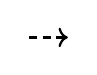
\begin{tikzpicture}[scale=0.8]\draw[->,densely dashed,thick] (0,0) to (0.62,0);\end{tikzpicture}}
\newcommand{\oneactbodyred}{\mathrel{\soneactbodyred}}
\newcommand{\soneactbodyredtc}{\pap{\soneactbodyred}{+}}
\newcommand{\oneactbodyredtc}{\mathrel{\soneactbodyredtc}} 
\newcommand{\soneactbodyredrtc}{\pap{\dashrightarrow}{*}}
\newcommand{\oneactbodyredrtc}{\mathrel{\soneactbodyredrtc}}             
  %\newcommand{\sconvoneactbodyred}{{\dashleftarrow}}
\newcommand{\sconvoneactbodyred}{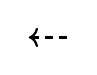
\begin{tikzpicture}[scale=0.8]\draw[<-,densely dashed,thick] (0,0) to (0.62,0);\end{tikzpicture}}
\newcommand{\convoneactbodyred}{\mathrel{\sconvoneactbodyred}}
\newcommand{\sconvoneactbodyredtc}{\pap{\sconvoneactbodyred}{+}}
\newcommand{\convoneactbodyredtc}{\mathrel{\soneactbodyredtc}} 
\newcommand{\sconvoneactbodyredrtc}{\pap{\sconvoneactbodyred}{*}}
\newcommand{\convoneactbodyredrtc}{\mathrel{\sconvoneactbodyredrtc}}

\newcommand{\snoonebodyred}{{\Rrightarrow}}
\newcommand{\noonebodyred}{\mathrel{\snoonebodyred}}
\newcommand{\snoonebodyredrc}{\pap{\snoonebodyred\hspace*{-1pt}}{=}}
\newcommand{\noonebodyredrc}{\mathrel{\snoonebodyredrc}} 
\newcommand{\sconvnoonebodyred}{{\Lleftarrow}}
\newcommand{\convnoonebodyred}{\mathrel{\sconvnoonebodyred}}
\newcommand{\sconvnoonebodyredrc}{\pap{\sconvnoonebodyred}{=}}
\newcommand{\convnoonebodyredrc}{\mathrel{\sconvnoonebodyredrc}}   
  






\newcommand{\sLebn}{\textit{Lebn}}
\newcommand{\Lebn}{\tfap{\sLebn}}
\newcommand{\Lebnext}[6]{\sLebn({#1},\hspace*{0.5pt}{#2},\hspace*{0.5pt}{#3};\hspace*{0.5pt}{#4},\hspace*{0.5pt}{#5},\hspace*{0.5pt}{#6})}
%
\newcommand{\sLebni}[1]{{\textit{Lebn-}{#1}}}
\newcommand{\Lebni}[1]{\tfap{\sLebni{#1}}}
%
\newcommand{\ebnLi}[2]{\tfap{#1}{#2}}
%



% one-step removal rewrite relations
% 
  \newcommand{\specfontsize}{\fontsize{5}{6}\selectfont} 
  %\newcommand{\subotr}{\hspace*{-1pt}\mbox{\specfontsize $(\hspace*{-0.6pt}\sone\hspace*{-0.85pt})$}}
  \newcommand{\subotr}{\hspace*{-1pt}{\scriptscriptstyle (\sone)}}
  \newcommand{\suboneprefixed}{{\hspace*{-1pt}\mbox{\specfontsize $(\hspace*{-0.6pt}\sone{\cdot}\hspace*{-0.85pt})$}}}
\newcommand{\sonestepremred}{\sredi{\subotr}}
\newcommand{\onestepremred}{\redi{\subotr}}
%
\newcommand{\sotelimred}{\sredb{\subotr}}
\newcommand{\otelimred}{\mathrel{\sotelimred}}
%
\newcommand{\sotelimredrtc}{\sredbp{\subotr}{*}}
\newcommand{\otelimredrtc}{\mathrel{\sotelimredrtc}}
\newcommand{\sotelimredtc}{\sredbp{\subotr}{+}}
\newcommand{\otelimredtc}{\mathrel{\sotelimredtc}}
%
\newcommand{\sotelimconvred}{\sconvredb{\subotr}}
\newcommand{\otelimconvred}{\mathrel{\sotelimconvred}}
\newcommand{\sotelimconvredrtc}{\sconvredbp{\subotr}{*}}
\newcommand{\otelimconvredrtc}{\mathrel{\sotelimconvredrtc}}



%
\newcommand{\sotrconvredrtc}{\sconvredbp{\subotr}{*}}
\newcommand{\otrconvredrtc}{\mathrel{\sotrconvredrtc}}
\newcommand{\sotrconvredtc}{\sconvredbp{\subotr}{+}}
\newcommand{\otrconvredtc}{\mathrel{\sotrconvredtc}}
%
\newcommand{\sotrconvred}{\sconvredi{\subotr}}
\newcommand{\otrconvred}{\convredi{\subotr}}
\newcommand{\sotrconvmred}{\sconvmredi{\subotr}}
\newcommand{\otrconvmred}{\convmredi{\subotr}}
\newcommand{\sotrmred}{{\smredi{\subotr}}}
\newcommand{\otrmred}{\mredi{\subotr}}
%
\newcommand{\sotelimredrstc}{{\sredrstci{\subotr}}}
\newcommand{\otelimredrstc}{\mathrel{\sotelimredrstc}}
%
% one-step removal equivalence
\newcommand{\sotreq}{{\sim_{\subotr}}}
\newcommand{\otreq}{\mathrel{\sotreq}}


% elim-red
\newcommand{\selim}{\mathrm{elim}}
\newcommand{\selimred}{{\to_{\selim}}}
\newcommand{\elimred}{\mathrel{\selimred}}
\newcommand{\snotelimred}{{\nrightarrow}_{\selim}}
\newcommand{\notelimred}{\hspace*{1pt}\snotelimred}
\newcommand{\selimmred}{\twoheadrightarrow_{\selim}}%{{\to_{\selim}^*}}
\newcommand{\elimmred}{\mathrel{\selimmred}}
\newcommand{\selimeqred}{{\bpap{\to}{\selim}{=}}}
\newcommand{\elimeqred}{\mathrel{\selimeqred}}
%
\newcommand{\sconvelimred}{{\leftarrow_{\selim}}}
\newcommand{\convelimred}{{\mathrel{\sconvelimred}}}
\newcommand{\sconvelimmred}{\twoheadleftarrow_{\selim}}%{\leftarrow_{\selim}^*}
\newcommand{\convelimmred}{\mathrel{\sconvelimmred}}
\newcommand{\sconvelimeqred}{{\bpap{\leftarrow}{\selim}{=}}}
\newcommand{\convelimeqred}{\mathrel{\sconvelimeqred}}
%
\newcommand{\selimnfred}{{\downarrow_{\selim}}}
\newcommand{\elimnfred}{\selimnfred}
%\newcommand{\elimnfredof}[1]{{#1}\selimnfred}

% elim-plus-red
\newcommand{\selimplus}{{\mathrm{elim}^+}}
\newcommand{\selimplusred}{{\to_{\selimplus}}}
\newcommand{\elimplusred}{\mathrel{\selimplusred}}
\newcommand{\snotelimplusred}{{\not\hspace*{-0.5pt}\to}_{\selimplus}}
\newcommand{\notelimplusred}{\hspace*{1pt}\snotelimplusred}
\newcommand{\selimplusmred}{{\to_{\selimplus}^*}}
\newcommand{\elimplusmred}{\mathrel{\selimplusmred}}
\newcommand{\selimpluseqred}{{\bpap{\to}{\selimplus}{=}}}
\newcommand{\elimpluseqred}{\mathrel{\selimpluseqred}}
%
\newcommand{\sconvelimplusred}{{\leftarrow_{\selimplus}}}
\newcommand{\convelimplusred}{{\mathrel{\sconvelimplusred}}}
\newcommand{\sconvelimplusmred}{\leftarrow_{\selimplus}^*}
\newcommand{\convelimplusmred}{\mathrel{\sconvelimplusmred}}
\newcommand{\sconvelimpluseqred}{{\bpap{\leftarrow}{\selimplus}{=}}}
\newcommand{\convelimpluseqred}{\mathrel{\sconvelimpluseqred}}
%
\newcommand{\selimplusnfred}{{\downarrow_{\selimplus}}}
\newcommand{\elimplusnfred}{\selimplusnfred}
%\newcommand{\elimnfredof}[1]{{#1}\selimnfred}



% prune-red
\newcommand{\sprune}{\mathrm{prune}}
\newcommand{\sprunered}{{\to_{\sprune}}}
\newcommand{\prunered}{\mathrel{\sprunered}}
\newcommand{\sprunemred}{{\to_{\sprune}^*}}
\newcommand{\prunemred}{\mathrel{\sprunemred}}
\newcommand{\spruneeqred}{{\to^{=}_{\sprune}}}
\newcommand{\pruneeqred}{\mathrel{\spruneeqred}}
%
\newcommand{\sconvprunered}{{\leftarrow_{\sprune}}}
\newcommand{\convprunered}{\mathrel{\sconvprunered}}
\newcommand{\sconvpruneeqred}{{\leftarrow^{=}_{\sprune}}}
\newcommand{\convpruneeqred}{\mathrel{\sconvpruneeqred}}
\newcommand{\sconvprunemred}{{\leftarrow_{\sprune}^*}}
\newcommand{\convprunemred}{\mathrel{\sconvprunemred}}

% elim-prune-red
\newcommand{\sep}{\mathrm{ep}}
\newcommand{\sepred}{{\to_{\sep}}}
\newcommand{\epred}{\mathrel{\sepred}}
\newcommand{\sepmred}{{\to_{\sep}^*}}
\newcommand{\epmred}{\mathrel{\sepmred}}
\newcommand{\snotepred}{{\nrightarrow}_{\sep}}
\newcommand{\notepred}{\hspace*{1pt}\snotepred}
\newcommand{\sepeqred}{{\bpap{\to}{\sep}{=}}}
\newcommand{\epeqred}{\mathrel{\sepeqred}}
%
\newcommand{\sconvepred}{{\leftarrow_{\sep}}}
\newcommand{\convepred}{\mathrel{\sconvepred}}
\newcommand{\sconvepmred}{{\leftarrow_{\sep}^*}}
\newcommand{\convepmred}{\mathrel{\sconvepmred}}
\newcommand{\sconvepeqred}{{\bpap{\leftarrow}{\sep}{=}}}
\newcommand{\convepeqred}{\mathrel{\sconvepeqred}}

% decouplered
\newcommand{\sdecouple}{\mathrm{dec}}
\newcommand{\sdecouplered}{{\iap{\to}{\sdecouple}}}
\newcommand{\decouplered}{\mathrel{\sdecouplered}}
\newcommand{\sdecouplemred}{{\bpap{\to}{\sdecouple}{*}}}
\newcommand{\decouplemred}{\mathrel{\sdecouplemred}}
\newcommand{\sdecoupleeqred}{{\bpap{\to}{\sdecouple}{=}}}
\newcommand{\decoupleeqred}{\mathrel{\sdecoupleeqred}}
%
\newcommand{\sconvdecouplered}{{\iap{\leftarrow}{\sdecouple}}}
\newcommand{\convdecouplered}{\mathrel{\sconvdecouplered}}
\newcommand{\sconvdecouplemred}{{\bpap{\leftarrow}{\sdecouple}{*}}}
\newcommand{\convdecouplemred}{\mathrel{\sconvdecouplemred}}
\newcommand{\sconvdecoupleeqred}{{\bpap{\leftarrow}{\sdecouple}{=}}}
\newcommand{\convdecoupleeqred}{\mathrel{\sconvdecoupleeqred}}
%
\newcommand{\sdecouplezero}{\mathrm{dec}_0}
\newcommand{\sdecouplezerored}{{\iap{\to}{\sdecouplezero}}}
\newcommand{\decouplezerored}{\mathrel{\sdecouplezerored}}
\newcommand{\sdecouplezeromred}{{\bpap{\to}{\sdecouplezero}{*}}}
\newcommand{\decouplezeromred}{\mathrel{\sdecouplezerored}}
\newcommand{\sdecouplezeroeqred}{{\bpap{\to}{\sdecouplezero}{=}}}
\newcommand{\decouplezeroeqred}{\mathrel{\sdecouplezeroeqred}}
%
\newcommand{\sconvdecouplezerored}{{\iap{\leftarrow}{\sdecouplezero}}}
\newcommand{\convdecouplezerored}{\mathrel{\sconvdecouplezerored}}
\newcommand{\sconvdecouplezeromred}{{\bpap{\leftarrow}{\sdecouplezero}{*}}}
\newcommand{\convdecouplezeromred}{\mathrel{\sconvdecouplezerored}}
\newcommand{\sconvdecouplezeroeqred}{{\bpap{\leftarrow}{\sdecouplezero}{=}}}
\newcommand{\convdecouplezeroeqred}{\mathrel{\sconvdecouplezeroeqred}}




% down, back, body, enter, branch step relations
% 
\newcommand{\sdownintostep}{\textit{din}}
\newcommand{\sbackstep}{\textit{back}}
\newcommand{\sdownstep}{\textit{down}}
\newcommand{\sintostep}{\textit{into}}
\newcommand{\sselfstep}{\textit{self}}
\newcommand{\sbranchstep}{\branchsteplab}
%
\newcommand{\sdownintored}{\sredi{\hspace*{-0.5pt}\sdownintostep}}
\newcommand{\sbackred}{\sredi{\sbackstep}}
\newcommand{\sdownred}{\sredi{\hspace*{-0.5pt}\sdownstep}}
\newcommand{\sintored}{\sredi{\sintostep}}
\newcommand{\sselfred}{\sredi{\hspace*{-0.5pt}\sselfstep}}
\newcommand{\sbranchred}{\sredi{\sbranchstep}}
%
\newcommand{\downintored}{\mathrel{\sdownintored}}
\newcommand{\backred}{\mathrel{\sbackred}}
\newcommand{\downred}{\mathrel{\sdownred}}
\newcommand{\intored}{\mathrel{\sintored}}
\newcommand{\selfred}{\mathrel{\sselfred}}
\newcommand{\branchred}{\mathrel{\sbranchred}}
%
\newcommand{\sdownintoredrtc}{\sredrtci{\hspace*{-0.5pt}\sdownintostep}}
\newcommand{\sbackredrtc}{\sredrtci{\sbackstep}}
\newcommand{\sdownredrtc}{\sredrtci{\hspace*{-0.5pt}\sdownstep}}
\newcommand{\sintoredrtc}{\sredrtci{\sstep}}
\newcommand{\sselfredrtc}{\sredrtci{\hspace*{-0.5pt}\sselfstep}}
\newcommand{\sbranchredrtc}{\sredrtci{\sbranchstep}}
%
\newcommand{\downintoredrtc}{\mathrel{\sdownintoredrtc}}
\newcommand{\backredrtc}{\mathrel{\sbackredrtc}}
\newcommand{\downredrtc}{\mathrel{\sdownredrtc}}
\newcommand{\intoredrtc}{\mathrel{\sintoredrtc}}
\newcommand{\selfredrtc}{\mathrel{\sselfredrtc}}
\newcommand{\branchredrtc}{\mathrel{\sbranchredrtc}}
%
\newcommand{\sdownintoredtc}{\sredtci{\hspace*{-0.5pt}\sdownintostep}}
\newcommand{\sbackredtc}{\sredtci{\sbackstep}}
\newcommand{\sdownredtc}{\sredtci{\hspace*{-0.5pt}\sdownstep}}
\newcommand{\sintoredtc}{\sredtci{\senterstep}}
\newcommand{\sselfredtc}{\sredtci{\hspace*{-0.5pt}\sselfstep}}
\newcommand{\sbranchredtc}{\sredtci{\sbranchstep}}
%
\newcommand{\downintoredtc}{\mathrel{\sdownintoredtc}}
\newcommand{\backredtc}{\mathrel{\sbackredtc}}
\newcommand{\downredtc}{\mathrel{\sdownredtc}}
\newcommand{\intoredtc}{\mathrel{\sintoredtc}}
\newcommand{\selfredtc}{\mathrel{\sselfredtc}}
\newcommand{\branchredtc}{\mathrel{\sbranchredtc}}
%



%% sets
\newcommand{\descsetexpmid}{\mathrel{\vert}}
\newcommand{\descsetexpbigmid}{\mathrel{\big\vert}}
\newcommand{\descsetexpBigmid}{\mathrel{\Big\vert}}
\newcommand{\descsetexpBiggmid}{\mathrel{\Bigg\vert}}
\newcommand{\descsetexp}[2]{\left\{{#1}\descsetexpmid{#2}\right\}}
\newcommand{\descsetexpnormalsize}[2]{\{{#1}\descsetexpmid{#2}\}}
\newcommand{\descsetexpns}[2]{\{{#1}\descsetexpmid{#2}\}}
\newcommand{\descsetexpbig}[2]{\bigl\{{#1}\descsetexpbigmid{#2}\bigr\}}
\newcommand{\descsetexpBig}[2]{\Bigl\{{#1}\descsetexpBigmid{#2}\Bigr\}}
\newcommand{\descsetexpBigg}[2]{\Biggl\{{#1}\descsetexpBigmid{#2}\Biggr\}}

\newcommand{\aset}{A}
\newcommand{\bset}{B}
\newcommand{\cset}{C}
\newcommand{\dset}{D}
\newcommand{\aseti}{\iap{\aset}}
\newcommand{\bseti}{\iap{\bset}}
\newcommand{\cseti}{\iap{\cset}}
\newcommand{\dseti}{\iap{\dset}}

\newcommand{\aclass}{C}
\newcommand{\aclassi}{\iap{\aclass}}  

\newcommand{\restrictto}[2]{{#1}\bap{{\mid}}{#2}}
\newcommand{\restricttoto}[3]{{#1}\bpap{{\mid}}{#2}{#3}}

\newcommand{\salabfun}{\widehat{(\cdot)}}
\newcommand{\alabfunsap}{\fap{\salabfun}}
\newcommand{\alabfun}[1]{\widehat{{#1}}}
%
\newcommand{\salabfunof}{\iap{\salabfun}}
\newcommand{\alabfunofsap}[1]{\fap{\salabfunof{#1}}}
\newcommand{\alabfunof}[2]{\bap{\alabfun{(#2)}}{#1}}

\newcommand{\conservativewrt}[1]{{$#1$}\nb-con\-ser\-va\-tive} 


\newcommand{\sdom}{\text{\nf dom}}
\newcommand{\domof}{\fap{\sdom}}
\newcommand{\scodom}{\text{\nf cod}}
\newcommand{\codomof}{\fap{\scodom}}
\newcommand{\scod}{\text{\nf cod}}
\newcommand{\codof}{\fap{\scod}}
\newcommand{\sran}{\text{\nf ran}}
\newcommand{\ranof}{\fap{\sran}}
\newcommand{\simg}{\text{\nf im}}
\newcommand{\imgof}{\fap{\simg}}
%
\newcommand{\sdomain}{\text{\nf dom}}
\newcommand{\domainof}{\fap{\sdomain}}
\newcommand{\scodomain}{\text{\nf cod}}
\newcommand{\codomainof}{\fap{\scodomain}}
\newcommand{\srange}{\text{\nf ran}}
\newcommand{\rangeof}{\fap{\srange}}
\newcommand{\simage}{\text{\nf im}}
\newcommand{\imageof}{\fap{\simage}}

\newcommand{\adomain}{{D}}
\newcommand{\adomaini}{\iap{\adomain}}


\newcommand{\sdiffset}{\textit{Diff\hspace*{1pt}}}
\newcommand{\diffset}[2]{\fap{\sdiffset}{{#1},{#2}}}

%-----------
%% relations
%----------- 
\newcommand{\sabrel}{R}
\newcommand{\abrel}{\mathrel{\sabrel}}

% equality relation, see rewrite relations
\newcommand{\saeqrel}{{\sim}}
\newcommand{\aeqrel}{\mathrel{\saeqrel}}
\newcommand{\saeqrelacc}{{\saeqrel'}}
\newcommand{\aeqrelacc}{\mathrel{\saeqrelacc}}

\newcommand{\inv}[1]{{#1}^{-1}}
\newcommand{\sbinrelconv}[1]{\breve{#1}}
\newcommand{\binrelconv}[1]{\mathrel{\sbinrelconv{#1}}}
\newcommand{\sbinrelit}[1]{{#1}^{*}}
\newcommand{\binrelit}[1]{\mathrel{\sbinrelit{#1}}}
\newcommand{\sbinrelpit}[1]{{#1}^{+}}
\newcommand{\binrelpit}[1]{\mathrel{\sbinrelpit{#1}}}
\newcommand{\sbinrelitn}[2]{{#2}^{#1}}
\newcommand{\binrelitn}[2]{\mathrel{\sbinrelitn{#1}{#2}}}
\newcommand{\sbinrelcomp}[2]{{#1}\cdot{#2}}
\newcommand{\binrelcomp}[2]{\mathrel{\sbinrelcomp{#1}{#2}}}




%-----------
%% functions
%----------- 
\newcommand{\safun}{f}
\newcommand{\afun}{\fap{\safun}}
\newcommand{\safuni}{\iap{\safun}}
\newcommand{\afuni}[1]{\fap{\safuni{#1}}}
%
\newcommand{\safunext}{\underline{\safun}}
\newcommand{\afunext}{\fap{\safunext}}
%
\newcommand{\saonefun}{\underline{\safun}}
\newcommand{\aonefun}{\fap{\saonefun}}
%%
\newcommand{\sbfun}{g}
\newcommand{\bfun}{\fap{\sbfun}}
\newcommand{\sbfuni}{\iap{\sbfun}}
\newcommand{\bfuni}[1]{\fap{\sbfuni{#1}}}
%
\newcommand{\sbfunext}{\overline{\sbfun}}
\newcommand{\bfunext}{\fap{\sbfunext}}
%
\newcommand{\sbonefun}{\overline{\sbfun}}
\newcommand{\bonefun}{\fap{\sbonefun}}
%
% 
\newcommand{\sdescfun}{\textit{desc}}
\newcommand{\descfun}{\fap{\sdescfun}}
\newcommand{\sdescfunext}{\overline{\textit{desc}}}
\newcommand{\descfunext}{\fap{\sdescfunext}}


\newcommand{\stransposition}{\mathsf{t}}
\newcommand{\stranspositionof}{\fap{\stransposition}}
\newcommand{\transpositionof}[1]{\fap{\stranspositionof{#1}}}




%%
%%
\newcommand{\sphifun}{\phi}
\newcommand{\phifun}{\fap{\sphifun}}
\newcommand{\sphifuni}{\iap{\sphifun}}
\newcommand{\phifuni}[1]{\fap{\sphifuni{#1}}}
\newcommand{\spsifun}{\psi}
\newcommand{\psifun}{\fap{\spsifun}}


\newcommand{\scompfuns}[2]{{#1}\circ{#2}}
\newcommand{\compfuns}[2]{\fap{\scompfuns{#1}{#2}}}

% partial functions
% 
\newcommand{\sundefd}{{\uparrow}}





% relations
% 
\newcommand{\sabinrel}{{R}}
\newcommand{\abinrel}{\mathrel{\sabinrel}}
\newcommand{\sabinrelacc}{\sabinrel'}
\newcommand{\abinrelacc}{\mathrel{\sacc}}
\newcommand{\sbbinrel}{{S}}
\newcommand{\bbinrel}{\mathrel{\sbbinrel}}
\newcommand{\scbinrel}{{T}}
\newcommand{\cbinrel}{\mathrel{\scbinrel}}

\newcommand{\sabinreli}[1]{{\iap{\sabinrel}{#1}}}
\newcommand{\abinreli}[1]{\mathrel{\sabinreli{#1}}}

\newcommand{\seqrelgenby}[1]{{\iap{\sim}{#1}}}
\newcommand{\eqrelgenby}[1]{\mathrel{\seqrelgenby{#1}}}
%
\newcommand{\seqrelgenbyon}[2]{{\bpap{\sim}{#1}{\scriptscriptstyle (#2)}}}
\newcommand{\eqrelgenbyon}[2]{\mathrel{\seqrelgenbyon{#1}{#2}}}



%% set expressions
\newcommand{\setexp}[1]{\left\{{#1}\right\}}
\newcommand{\setexpnormalsize}[1]{\{{#1}\}}
\newcommand{\setexpbig}[1]{\bigl\{{#1}\bigr\}}
\newcommand{\setexpBig}[1]{\Bigl\{{#1}\Bigr\}}
\newcommand{\setexpBigg}[1]{\Biggl\{{#1}\Biggr\}}
%%
\newcommand{\spowersetof}{{\cal P}}
\newcommand{\powersetof}{\fap{\spowersetof}}
\newcommand{\factorset}[2]{{#1}/_{#2}}
%
\renewcommand{\emptyset}{\varnothing}

\newcommand{\mysetminus}{\hspace*{1pt}{\setminus}\hspace*{0.5pt}}

\newcommand{\toset}{\fap{\text{\nf set}}}

\newcommand{\Sets}{\textsf{Sets}}



% vectors
\newcommand{\vectexp}[1]{\tuple{#1}}

\newcommand{\vect}{\vv}

%
% logic
\newcommand{\slogand}{\wedge}
\newcommand{\slogor}{\vee}
\newcommand{\logand}{\mathrel{\slogand}}
\newcommand{\logor}{\mathrel{\slogor}} 
\newcommand{\slognot}{\neg}
\newcommand{\lognot}[1]{\slognot{#1}}

\newcommand{\existsst}[2]{\exists{\hspace*{1pt}#1}{#2}}
\newcommand{\uniqueexistsst}[2]{\exists{!}{\hspace*{1pt}#1}{#2}}
\newcommand{\forallst}[2]{\forall{\hspace*{0.5pt}#1}{#2}}
\newcommand{\existsstzero}[1]{\exists{\hspace*{1pt}#1}}
\newcommand{\uniqueexistsstzero}[1]{\exists{!}{\hspace*{1pt}#1}}
\newcommand{\forallstzero}[1]{\forall{\hspace*{0.5pt}#1}}

% words
% 
\newcommand{\salph}{\textit{Alph}}
% 
\newcommand{\aalph}{A}
\newcommand{\balph}{B}

\newcommand{\alphi}{\iap{\salph}}
\newcommand{\alphiof}[1]{\fap{\alphi{#1}}}





% 
% 
\newcommand{\emptyword}{\epsilon}

\newcommand{\finwordsover}[1]{#1 ^*}
\newcommand{\nonemptyfinwordsover}[1]{#1 ^+}
\newcommand{\infwordsover}[1]{#1 ^{\omega}}
\newcommand{\wordsover}[1]{#1 ^{\infty}}

\newcommand{\aiw}{\sigma}
\newcommand{\biw}{\rho}
\newcommand{\ciw}{\xi}

\newcommand{\wrdcns}[2]{{#1}\cdot{#2}}
\newcommand{\wrdcnse}[2]{{#1}{#2}}



\newcommand{\prefix}[2]{{#1}\hspace*{0.5pt}{\uparrow}^{#2}}
\newcommand{\suffix}[2]{{#1}\hspace*{0.5pt}{\uparrow}_{#2}}
\newcommand{\subword}[3]{{#1}\hspace*{0.5pt}{\uparrow}_{#2}^{#3}}

\newcommand{\length}[1]{\left|{#1}\right|}
\newcommand{\lengthbig}[1]{\bigl|{#1}\bigr|}
\newcommand{\lengthBig}[1]{\Bigl|{#1}\Bigr|}

\newcommand{\height}[1]{\left|{#1}\right|}
\newcommand{\heightbig}[1]{\bigl|{#1}\bigr|}
\newcommand{\heightBig}[1]{\Bigl|{#1}\Bigr|}

\newcommand{\depth}{\length}
\newcommand{\depthbig}{\lengthbig}
\newcommand{\depthBig}{\lengthBig}



\newcommand{\sprefixorder}{\sqsubseteq}
\newcommand{\sstrictprefixorder}{\sqsubset}
\newcommand{\sconvprefixorder}{\sqsupseteq}
\newcommand{\sconvstrictprefixorder}{\sqsupset}
%
\newcommand{\sisprefof}{\sprefixorder}
\newcommand{\isprefof}{\mathrel{\sisprefof}}
%
\newcommand{\shaspref}{\sconvprefixorder}
\newcommand{\haspref}{\mathrel{\shaspref}}
%
\newcommand{\sispropprefof}{\sstrictprefixorder}
\newcommand{\ispropprefof}{\mathrel{\sispropprefof}}
%
\newcommand{\shasproppref}{\sconvprefixorder}
\newcommand{\hasproppref}{\mathrel{\shasproppref}}

\newcommand{\subscriptprefixorder}{{\scalebox{0.62}{$\sqsubseteq$}}}
\newcommand{\sisparentof}{\to_{\subscriptprefixorder}}
\newcommand{\isparentof}{\mathrel{\sisparentof}}

\newcommand{\treeover}{\fap{\mathcal{T}}}


% tight fbox
%
\newcommand{\tightfbox}[1]{{\fboxsep=1.5pt\fbox{#1}}}


% FSTs
\newcommand{\aFST}{T}





% word abbreviations
% 
\newcommand{\ARS}{ARS}
\newcommand{\ARSs}{\ARS{s}}

\newcommand{\associatedprocess}{as\-so\-ci\-at\-ed-pro\-cess}

\newcommand{\nary}[1]{${#1}$\nb-ary}

%\newcommand{\actionprefix}{ac\-tion-pre\-fix}
\newcommand{\headaction}{head-ac\-tion}

\newcommand{\actionderivative}{action derivative}
\newcommand{\actionderivatives}{\actionderivative{s}}
\newcommand{\actiontickderivative}{action--tick-derivative}
\newcommand{\actiontickderivatives}{\actiontickderivative{s}}

\newcommand{\alphaconversion}{$\alpha$\nb-con\-ver\-sion}


\newcommand{\backbinding}{back-link}%{back\nb-bin\-ding}
\newcommand{\backbindings}{\backbinding{s}}
\newcommand{\Backbinding}{Back\nb-bin\-ding}
\newcommand{\Backbindings}{\Backbinding{s}}
\newcommand{\bisimulationcollapsed}{bi\-si\-mu\-la\-tion-col\-lapsed}
\newcommand{\onebisimulationcollapsed}{$\sone$-bi\-si\-mu\-la\-tion-col\-lapsed}
\newcommand{\onebisimulationcollapsedbf}{$\boldsymbol{\sone}$-bi\-si\-mu\-la\-tion-col\-lapsed}

\newcommand{\bisimilaritycollapsed}{bi\-si\-mu\-la\-ri\-ty-col\-lapsed}
\newcommand{\onebisimilaritycollapsed}{$\sone$\nb-bi\-si\-mi\-la\-rity-col\-lapsed}
\newcommand{\onebisimilaritycollapsedbf}{$\boldsymbol{\sone}$\nb-bi\-si\-mi\-la\-rity-col\-lapsed}
\newcommand{\onebisimcollapsed}{$\sbisimos$\hspace*{-1pt}\nb-col\-lapsed}
\newcommand{\onebisimcollapsedbf}{$\boldsymbol{\sbisimos}$\hspace*{-1pt}\nb-col\-lapsed}


\newcommand{\backlink}{backlink}
\newcommand{\backlinks}{\backlink{s}}
\newcommand{\onebacklink}{$\sone$\nb-\backlink}
\newcommand{\onebacklinks}{$\sone$\nb-\backlink{s}}

\newcommand{\biimplication}{bi-impli\-ca\-tion}
\newcommand{\biimplications}{\biimplication{s}}

\newcommand{\biinterpretable}{bi-inter\-pret\-able}
\newcommand{\biinterpretability}{bi-inter\-pret\-a\-bi\-li\-ty}

\newcommand{\bisimulationsubsumed}{bi\-si\-mu\-la\-tion-sub\-sumed}

\newcommand{\bireachable}{bi-reach\-able}
\newcommand{\bireachability}{bi-reach\-abi\-li\-ty}

\newcommand{\bodypart}{bo\-dy-part}

\newcommand{\bottomup}{bot\-tom-up}


\newcommand{\branchstep}{branch-step}
\newcommand{\body}{body-step}


\newcommand{\casedistinction}{case-dis\-tinc\-tion}

\newcommand{\chartone}{\mbox{chart$^{(\sone)}$}}
\newcommand{\chartsone}{\mbox{charts$^{(\sone)}$}}

\newcommand{\channeleager}{chan\-nel-ea\-ger}

\newcommand{\coinitial}{co-ini\-tial}

\newcommand{\cyclesymmetric}{cy\-cle-sym\-metric}
\newcommand{\permutationsymmetric}{per\-mu\-ta\-tion-sym\-metric}
\newcommand{\permutationsymmetrically}{per\-mu\-ta\-tion-sym\-metri\-cally}

\newcommand{\downwardsclosed}{down\-ward-closed}


\newcommand{\collapsedwrt}[1]{{$#1$}\nb-col\-lapsed}
\newcommand{\pseudocollapsedwrt}[1]{pseu\-do-\collapsedwrt{#1}}
\newcommand{\nearcollapsedwrt}[1]{near-\collapsedwrt{#1}}
%
\newcommand{\collapsewrt}[1]{{$#1$}\nb-col\-lapsed}
\newcommand{\pseudocollapsewrt}[1]{pseu\-do-\collapsewrt{#1}}
\newcommand{\nearcollapsewrt}[1]{near-\collapsewrt{#1}} 

\newcommand{\nearcollapsing}{near-col\-lapsing}

\newcommand{\noncoinciding}{non-co\-in\-ci\-ding}

\newcommand{\faithfulwrt}[1]{${#1}$-faith\-ful}



\newcommand{\shadowedB}[1]{${#1}$\nb-shad\-owed}
\newcommand{\shadowsB}[1]{${#1}$\nb-shad\-ows}
\newcommand{\shadowingB}[1]{${#1}$\nb-shad\-ow\-ing}
%
\newcommand{\mimickedB}[1]{${#1}$\nb-mim\-icked}
\newcommand{\mimicsB}[1]{${#1}$\nb-mim\-ics}
\newcommand{\mimickingB}[1]{${#1}$\nb-mim\-icking}

\newcommand{\languageequivalent}{lan\-guage-equiv\-a\-lent}

\newcommand{\cyclefreeness}{cycle-free\-ness}




\newcommand{\derivativesgenerated}{de\-riv\-a\-tives-ge\-ne\-ra\-ted}
\newcommand{\derivativesbased}{de\-riv\-a\-tives-based}

\newcommand{\directsuccessor}{di\-rect-suc\-ces\-sor}
\newcommand{\directsuccessorwrt}[1]{di\-rect-{$#1$}-suc\-ces\-sor}


\newcommand{\wderivative}[1]{{$#1$}\nb-de\-riv\-a\-tive}
\newcommand{\wderivatives}[1]{\aderivative{#1}s}
\newcommand{\aderivative}[1]{{$#1$}\nb-de\-riv\-a\-tive}
\newcommand{\aderivatives}[1]{\aderivative{#1}s}

\newcommand{\Wcollapsed}[1]{{$#1$\hspace*{-1pt}}\nb-col\-lapsed}
\newcommand{\Wpseudocollapsed}[1]{{$#1$\hspace*{-1pt}}\nb-\pseudocollapsed{}}


\newcommand{\elementwise}{el\-e\-ment-wise}

\newcommand{\eqlogicextending}{$\eqlogic$\nb-ex\-tend\-ing}
\newcommand{\equationallogic}{equa\-ti\-onal-log\-ic}
\newcommand{\equationallogicbased}{\equationallogic-based}
\newcommand{\equationallogicextending}{\equationallogic-ex\-ten\-ding}
\newcommand{\eqlogicbased}{$\eqlogic$\nb-based}
\newcommand{\eqlogictheory}{$\eqlogic$\nb-the\-o\-ry}
\newcommand{\eqlogictheories}{$\eqlogic$\nb-the\-o\-ries}
\newcommand{\eqlogicbasedtheory}{$\eqlogic$\nb-based-the\-o\-ry}
\newcommand{\eqlogicbasedtheories}{$\eqlogic$\nb-based-the\-o\-ries}



\newcommand{\eqlogicproofsystem}{$\eqlogic$\nb-proof-system}

\newcommand{\equivalenceclasseswrt}[1]{${#1}$\nb-equivalence classes}


\newcommand{\exititeration}{ex\-it-it\-er\-a\-tion}

\newcommand{\entrytransition}{en\-try tran\-si\-tion}
\newcommand{\entrytransitions}{\entrytransition{s}}
\newcommand{\exittransition}{exit tran\-si\-tion}
\newcommand{\exittransitions}{\exittransition{s}}
\newcommand{\entrystep}{en\-try-step}
\newcommand{\entrysteps}{\entrystep{s}}

\newcommand{\exitpart}{ex\-it-part}

\newcommand{\extractablein}[1]{${#1}$\nb-ex\-tract\-able}
\newcommand{\extractedin}[1]{${#1}$\nb-ex\-tracted}
\newcommand{\extractionin}[1]{${#1}$\nb-ex\-trac\-tion}

\newcommand{\extractedfrom}[1]{${#1}$\nb-ex\-tracted}

\newcommand{\finitebaseswitnessed}{fi\-nitely-based}

\newcommand{\functionalbisimilarity}{func\-ti\-onal-bi\-si\-mi\-la\-rity}


\newcommand{\FST}{FST}
\newcommand{\FSTs}{\FST{s}}

\newcommand{\Fcoalgebra}[1]{{$#1$}\nb-co\-al\-ge\-bra}
\newcommand{\Fcoalgebras}[1]{\Fcoalgebra{#1}s}

\newcommand{\finitestate}{fi\-nite-state}

\newcommand{\functionsymbol}{func\-tion-sym\-bol}
\newcommand{\functionsymbols}{\functinsymbol{s}}
\newcommand{\Functionsymbol}{Func\-tion-sym\-bol}


\newcommand{\forthcondition}{forth-con\-di\-tion}
\newcommand{\backcondition}{back-con\-di\-tion}

\newcommand{\generatedby}[1]{${#1}$\nb-ge\-ne\-ra\-ted}

\newcommand{\generalizedloopexitchart}{ge\-ne\-ra\-lized-loop--ex\-it chart}
\newcommand{\gloopexitchart}{gloop--ex\-it chart}
\newcommand{\generalizedloopexitcharts}{\generalizedloopexitchart{s}}
\newcommand{\gloopexitcharts}{\gloopexitchart{s}}

\newcommand{\Hilbertstyle}{Hil\-bert-style}

\newcommand{\hgleform}{hgle\hspace*{0.35pt}-\hspace*{-0.4pt}form}
\newcommand{\hpleform}{hple\hspace*{0.35pt}-\hspace*{-0.4pt}form}
%
\newcommand{\glenormalform}{gle\hspace*{0.35pt}-\hspace*{-0.4pt}nor\-mal-form}
\newcommand{\glepanormalform}{glepa\hspace*{0.35pt}-\hspace*{-0.4pt}nor\-mal-form}
\newcommand{\lepanormalform}{lepa\hspace*{0.35pt}-\hspace*{-0.4pt}nor\-mal-form}


\newcommand{\ibnproperty}{ibn-prop\-erty}
\newcommand{\iterationbodynontermination}{it\-er\-a\-tion-bo\-dy-non-ter\-mi\-na\-tion}

\newcommand{\inducedtransition}{in\-duced-tran\-si\-tion}
\newcommand{\inducedtransitionsolution}{in\-duced-tran\-si\-tion-so\-lu\-tion}
\newcommand{\itrsolution}{itr\nb-so\-lu\-tion}

\newcommand{\immediatetermination}{im\-me\-di\-ate-ter\-mi\-na\-tion}



\newcommand{\rootconnected}{root-con\-nect\-ed}
\newcommand{\rootconnectedness}{root con\-nect\-ed\-ness}
\newcommand{\startconnected}{start-ver\-tex con\-nect\-ed}
\newcommand{\startconnectedness}{start-ver\-tex\ con\-nect\-ed\-ness}
\newcommand{\loopconnected}{loop-con\-nect\-ed}
\newcommand{\loopconnectedness}{loop-con\-nect\-ed\-ness}

\newcommand{\loopelimination}{loop\nb-elim\-i\-nat\-ion}
\newcommand{\entireloopelimination}{en\-tire-loop-elim\-i\-na\-tion}


\newcommand{\listconcatenation}{list-con\-ca\-te\-na\-tion}

\newcommand{\loopentryl}[1]{{$#1$}-loop-entry}
\newcommand{\loopexit}{loop--ex\-it}

\newcommand{\loopentryexitentry}{loop-en\-try--ex\-it-en\-try}


\newcommand{\loopexitchart}{loop--ex\-it chart}
\newcommand{\loopexitcharts}{\loopexitchart{s}}


\newcommand{\loopentry}{loop-en\-try}
\newcommand{\loopbody}{loop-body}




\newcommand{\loopuniform}{loop-uni\-form}
\newcommand{\branchuniform}{branch-uni\-form}
\newcommand{\txtloopsbackto}{loops-back-to}
\newcommand{\txtloopsbacktol}[1]{{$#1$}-\txtloopsbackto}
\newcommand{\txtLoopsbackto}{Loops-back-to}
\newcommand{\txtdirectlyloopsbackto}{di\-rectly-loops-back-to}
\newcommand{\txtdirectlyloopsbacktol}[1]{{$#1$}-\txtdirectlyloopsbackto}
\newcommand{\loopsbacktouniform}{\txtloopsbackto-uni\-form}
%
\newcommand{\loopbranchlabeling}{loop-branch-la\-be\-ling}
\newcommand{\loopbranchlabelings}{\loopbranchlabeling{s}}
\newcommand{\loopbranchlabelingover}[1]{{$#1$}\nb-\loopbranchlabeling}
\newcommand{\loopbranchlabelingsover}[1]{\loopbranchlabelingover{#1}s}
%
\newcommand{\entrybodylabeling}{en\-try\discretionary{/}{}{/}body-la\-be\-ling}
\newcommand{\entrybodylabelings}{\entrybodylabeling{s}}
\newcommand{\Entrybodylabeling}{En\-try\discretionary{/}{}{/}body-la\-be\-ling}
%
\newcommand{\looplabeling}{loop-la\-be\-ling}
\newcommand{\looplabelings}{\looplabeling{s}}
\newcommand{\looplabelingover}[1]{{$#1$}\nb-\looplabeling}
\newcommand{\looplabelingsover}[1]{\looplabelingover{#1}s}
\newcommand{\Llooplabeling}[1]{{$#1$}\nb-\looplabeling}
\newcommand{\Llooplabelings}[1]{\Llooplabeling{#1}s}

\newcommand{\LEEshape}{\LEE\nb-shape}
\newcommand{\LEEshapebf}{\LEEbf\nb-shape}
\newcommand{\LEEShape}{\LEE\nb-shape}
\newcommand{\LEEShapebf}{\LEEbf\nb-shape}
%
\newcommand{\LEEshaped}{\LEE\nb-shaped}
\newcommand{\LEEshapedbf}{\LEEbf\nb-shaped}
\newcommand{\LEEShaped}{\LEE\nb-Shaped}
\newcommand{\LEEShapedbf}{\LEEbf\nb-Shaped}

\newcommand{\LLEEpreserving}{\LLEE\nb-pre\-serving}
\newcommand{\LLEEpreservingly}{\LLEE\nb-pre\-servingly}
\newcommand{\LLEEpreservingbf}{\LLEEbf\nb-pre\-serving}
\newcommand{\LLEEPreserving}{\LLEE\nb-Pre\-serving}
\newcommand{\LLEEPreservingbf}{\LLEEbf\nb-Pre\-serving}
%
\newcommand{\LEEpreserving}{\LEE\nb-pre\-serving}
\newcommand{\LEEpreservingly}{\LEE\nb-pre\-ser\-vingly}
%
\newcommand{\LLEEpluspreserving}{\LLEEplus -pre\-serving}
\newcommand{\LLEEpluspreservingly}{\LLEEplus -pre\-servingly}
\newcommand{\LLEEpluspreservingbf}{\LLEEplusbf -pre\-serving}
\newcommand{\LLEEplusPreserving}{\LLEEplus -Pre\-serving}
\newcommand{\LLEEplusPreservingbf}{\LLEEplusbf -Pre\-serving}





\newcommand{\generalizedloop}{ge\-ne\-ral\-ized-loop}
\newcommand{\generalizedloopentry}{\generalizedloop-entry}
\newcommand{\generalizedloopexit}{\generalizedloop-exit}
\newcommand{\generalizedloopexits}{\generalizedloopexit{s}}

\newcommand{\generalizedloopentriesexitsbodynested}{ge\-ne\-ra\-lized-loop-en\-try-exits-body-nes\-ted}

\newcommand{\generalizedloopexitbranchlabeling}{ge\-ne\-ra\-lized-loop-exit-branch-la\-be\-ling}
\newcommand{\generalizedloopexitbranchlabelings}{\generalizedloopexitbranchlabeling{s}}
\newcommand{\generalizedloopexitbranchlabelingover}[1]{${#1}$\nb-ge\-ne\-ra\-lized-loop-exit-branch-la\-be\-ling}
\newcommand{\generalizedloopexitbranchlabelingsover}[1]{\generalizedloopexitbranchlabeling{#1}{s}}
%
\newcommand{\generalizedlooplabeling}{ge\-ne\-ra\-lized-loop-la\-be\-ling}
\newcommand{\generalizedlooplabelings}{\generalizedlooplabeling{s}}
\newcommand{\generalizedlooplabelingover}[1]{${#1}$\nb-\generalizedlooplabeling}
\newcommand{\generalizedlooplabelingsover}[1]{\generalizedlooplabeling{#1}{s}}
\newcommand{\Lgenlooplabeling}[1]{${#1}$\nb-\generalizedlooplabeling}
\newcommand{\Lgenlooplabelings}[1]{\generalizedlooplabeling{#1}{s}}




%
% 
% 
% 
% 
\newcommand{\Llabeling}[1]{{$#1$}\nb-la\-be\-ling}
\newcommand{\Llabelings}[1]{\Llabeling{#1}s}
\newcommand{\Llabeled}[1]{{$#1$}\nb-la\-be\-led}
%
\newcommand{\Lletterlabeling}[1]{{$#1$}\nb-let\-ter-la\-be\-ling}
\newcommand{\Lletterlabeled}[1]{{$#1$}\nb-let\-ter-la\-be\-led}
%
\newcommand{\Lpluslabeling}[1]{{$#1^+$\hspace*{-1.75pt}}\nb-la\-be\-ling}
\newcommand{\Lpluslabeled}[1]{{$#1^+$\hspace*{-1.75pt}}\nb-la\-be\-led}
%
\newcommand{\Lwordlabeling}[1]{{$#1$}\nb-word-la\-be\-ling}
\newcommand{\Lwordlabeled}[1]{{$#1$}\nb-word-la\-be\-led}

\newcommand{\lptc}{lpt\nb-chart}
\newcommand{\lptcs}{\lptc{s}}
\newcommand{\lsptc}{lspt\nb-chart}
\newcommand{\lsptcs}{\lsptc{s}}

\newcommand{\LEEexistswitness}{$\LEEexists$\nb-wit\-ness}
\newcommand{\LEEexistswitnessbf}{{$\LEEexistsbf$\nb-wit\-ness}}
\newcommand{\LEEwitness}{$\LEE$\nb-wit\-ness}
\newcommand{\LEEWitness}{$\LEE$\nb-Wit\-ness}
\newcommand{\LEEwitnessbf}{$\LEEbf$\hspace*{1pt}\nb-wit\-ness}
\newcommand{\LEEWitnessbf}{$\LEEbf$\hspace{1pt}\nb-Wit\-ness}
\newcommand{\LEEexistswitnesses}{$\LEEexists$\hspace*{1.25pt}\nb-wit\-nes\-ses}
\newcommand{\LEEexistswitnessesbf}{{$\LEEexistsbf$\hspace*{1.25pt}\nb-wit\-nes\-ses}}
\newcommand{\LEEwitnesses}{$\LEE$\hspace*{1.25pt}\nb-wit\-nes\-ses}
\newcommand{\LEEwitnessesbf}{$\LEEbf$\hspace*{1pt}\nb-wit\-nes\-ses}
\newcommand{\LEEWitnesses}{$\LEE$\hspace*{1pt}\nb-Wit\-nes\-ses}
\newcommand{\LEEWitnessesbf}{$\LEEbf$\hspace*{1pt}\nb-Wit\-nes\-ses}
%
\newcommand{\LLEEwitness}{{\nf LLEE}\nb-wit\-ness}
\newcommand{\LLEEwitnesses}{{\nf LLEE}\nb-wit\-nesses}
\newcommand{\LLEEwitnessemph}{\emph{LLEE\nb-wit\-ness}}
\newcommand{\LLEEchart}{{\nf LLEE}\nb-chart}
\newcommand{\LLEEchartemph}{\emph{LLEE\nb-chart}}
\newcommand{\LLEEcharts}{{\nf LLEE}\nb-chart{s}}

% \newcommand{\LLEEonewitness}{\LLEEone\nb-wit\-ness}
% \newcommand{\LLEEonewitnesses}{\LLEEonewitness{es}}
% \newcommand{\LLEEoneshaped}{\LLEEone\nb-shaped}

\newcommand{\LLEEonechart}{{\nf LLEE}\hspace*{1pt}-\onechart}
\newcommand{\LLEEonechartbf}{{LLEE}\hspace*{1pt}-\onechartbf}
% \newcommand{\LLEEonechartemph}{\emph{LLEE\hspace*{1pt}-\onechart}}
\newcommand{\LLEEonecharts}{{LLEE}\hspace*{1pt}-\onechart{s}}
\newcommand{\LLEEonechartsbf}{{LLEE}\hspace*{1pt}-\onechartbf{s}}
\newcommand{\wgLLEEonechart}{\text{\nf wg-LLEE}\hspace*{1pt}-\onechart}
%
\newcommand{\LLEEplusonechart}{{\LLEEplus}\hspace*{-0.5pt}-\onechart}
\newcommand{\LLEEplusonecharts}{{\LLEEplus}\hspace*{-0.5pt}-\onecharts}
\newcommand{\LLEEplusonechartbf}{{\LLEEplusbf}\hspace*{-0.5pt}-\onechartbf}
\newcommand{\LLEEplusonechartsbf}{{\LLEEplusbf}\hspace*{-0.5pt}-\onechartsbf}

\newcommand{\LLEEonelimchart}{\LLEEonelim-chart}






\newcommand{\milnersyssolvable}{$\milnersys$\nb-solvable}

\newcommand{\nonempty}{non-emp\-ty}
\newcommand{\nonexclusive}{non-ex\-clu\-sive}
\newcommand{\noexit}{no-ex\-it}

\newcommand{\nonbisimilar}{non-bi\-simi\-lar}
\newcommand{\nongrounded}{non-groun\-ded}
\newcommand{\nonproper}{non-pro\-per}
\newcommand{\nonlayered}{non-lay\-er\-ed}
\newcommand{\nonredundant}{non-re\-dun\-dant}
\newcommand{\nonlooping}{non-loo\-ping}
\newcommand{\nonoverlapping}{non-over-lap\-ping}
\newcommand{\nonsubsumed}{non-sub\-sumed}
\newcommand{\nonterminal}{non\-ter\-mi\-nal}
\newcommand{\nonterminalsymbol}{non\-ter\-mi\-nal symbol}
\newcommand{\nonterminalsymbols}{\nonterminalsymbol{s}}
\newcommand{\nonterminals}{\nonterminal{s}}
\newcommand{\nonvacuous}{non-vac\-u\-ous}
\newcommand{\nontrivial}{non-triv\-i\-al}
\newcommand{\nonzero}{non-zero}
\newcommand{\nonidentical}{non-iden\-ti\-cal}

\newcommand{\nonbody}{non-bo\-dy}
\newcommand{\noncollapsed}{non-col\-lapsed}
\newcommand{\nondeterministic}{non-de\-ter\-min\-istic}

\newcommand{\notlayered}{not-lay\-ered}
\newcommand{\notlayeredness}{not-lay\-ered\-ness}  

  
\newcommand{\nfof}[1]{$#1$\nb-nor\-mal form}
\newcommand{\nfsof}[1]{\nfof{#1}s}

\newcommand{\onebehavior}{$\sone$\nb-be\-hav\-ior}
\newcommand{\onebehaviorbf}{$\boldsymbol{\sone}$\nb-be\-hav\-ior}

\newcommand{\onemove}{$\sone$\nb-tran\-si\-tion}
\newcommand{\onestep}{$\sone$\nb-step}
\newcommand{\onesteps}{\onestep{s}}
\newcommand{\onestepbf}{$\boldsymbol{\sone}$\nb-step}
\newcommand{\onestepsbf}{\onestepbf{s}}
\newcommand{\onetransition}{$\sone$\nb-tran\-si\-tion}
\newcommand{\onetransitions}{\onetransition{s}}
\newcommand{\oneTransition}{$\sone$\nb-Tran\-si\-tion}
\newcommand{\oneTransitions}{\oneTransition{s}}
\newcommand{\onetransitionbf}{$\boldsymbol{\sone}$\nb-tran\-si\-tion}
\newcommand{\onetransitionsbf}{\onetransitionbf{s}}
\newcommand{\onetransitioninducedtermination}{\onetransition-in\-duced-ter\-mi\-na\-tion}
\newcommand{\onetransitionless}{\onetransition-less}
\newcommand{\onetransitionfree}{\onetransition-free}

\newcommand{\otr}{\onetransition}
\newcommand{\onetransitionrefinement}{refinement} %{\otr{} refinement}
\newcommand{\onetransitionrefinements}{\onetransitionrefinement{s}}
\newcommand{\onetransitionrefine}{refine} %{\otr{} refines}
\newcommand{\onetransitionrefines}{refines} %{\otr{} refines}
\newcommand{\onetransitionrefined}{refined} %{\otr{} refined}

\newcommand{\oneprefixed}{$\sone$\nb-pre\-fixed}
\newcommand{\onefree}{$\sone$\nb-free}
\newcommand{\oneless}{$\stexpone$\nb-less}
\newcommand{\oneLess}{$\stexpone$\nb-Less}
\newcommand{\quasioneless}{quasi-\oneless}
\newcommand{\Quasioneless}{Quasi-\oneless}
\newcommand{\Onefree}{$\sone$\nb-Free}
\newcommand{\onefreebf}{$\boldsymbol{\sone}$\nb-free}
\newcommand{\onecycle}{$\sone$\nb-cycle}
\newcommand{\onecycles}{\onecycle{s}}
\newcommand{\onechart}{$\sone$\nb-chart}
\newcommand{\oneChart}{$\sone$\nb-Chart}
\newcommand{\oneCharts}{\oneChart{s}}
\newcommand{\onecharts}{\onechart{s}}
\newcommand{\onechartbf}{$\boldsymbol{\sone}$\nb-chart}
\newcommand{\oneChartbf}{$\boldsymbol{\sone}$\nb-Chart}
\newcommand{\oneChartsbf}{\oneChart{s}}
\newcommand{\onechartsbf}{\onechartbf{s}}

\newcommand{\stexponefree}{1\nb-free}


\newcommand{\stchart}{st\nb-chart}
\newcommand{\stcharts}{\stchart{s}}

\newcommand{\onetermchart}{$\sone\hspace*{-0.75pt}\trms$\nb-chart}
\newcommand{\onetermcharts}{\onetermchart{s}}
\newcommand{\onetermchartbf}{$\boldsymbol{\sone}\hspace*{-0.5pt}\boldsymbol{\trms}$\nb-chart}
\newcommand{\onetermchartsbf}{\onetermchartbf{s}}
\newcommand{\onetermChart}{$\sone\hspace*{-0.75pt}\trms$\nb-Chart}
\newcommand{\onetermCharts}{\onetermChart{s}}



\newcommand{\oneexit}{$\sone$\nb-exit}
\newcommand{\oneexitfree}{\oneexit-free}
\newcommand{\oneexitbf}{$\boldsymbol{\sone}$\nb-exit}
\newcommand{\oneexitfreebf}{\oneexitbf-free}
\newcommand{\onesideexit}{$\sone$\nb-side-exit}
\newcommand{\onesideexitfree}{\onesideexit-free}
\newcommand{\onesideexitbf}{$\boldsymbol{\sone}$\nb-side-exit}
\newcommand{\onesideexitfreebf}{\onesideexitbf-free}

\newcommand{\oneprogress}{$\sone$\nb-prog\-ress}
\newcommand{\onebisimulation}{$\sone$\nb-bi\-si\-mu\-la\-tion}
\newcommand{\onebisimulations}{\onebisimulation{s}}
\newcommand{\onebisimulationbf}{$\boldsymbol{\sone}$\nb-bi\-si\-mu\-la\-tion}
\newcommand{\onebisimulationsbf}{\onebisimulationbf{s}}
  \newcommand{\selfonebisimulation}{self-$\sone$\nb-bi\-si\-mu\-la\-tion}
  \newcommand{\selfonebisimulations}{\selfonebisimulation{s}}
  \newcommand{\selfonebisimulationbf}{self-$\boldsymbol{\sone}$\nb-bi\-si\-mu\-la\-tion}
  \newcommand{\selfonebisimulationsbf}{\selfonebisimulationbf{s}}  
\newcommand{\onebisimilar}{$\sone$\nb-bi\-si\-mi\-lar}
\newcommand{\oneBisimilar}{$\sone$\nb-Bi\-si\-mi\-lar}
\newcommand{\onebisimilarbf}{$\boldsymbol{\sone}$\nb-bi\-si\-mi\-lar}
\newcommand{\onebisimilarity}{$\sone$\nb-bi\-si\-mi\-la\-ri\-ty}
\newcommand{\onebisimilaritybf}{$\boldsymbol{\sone}$\nb-bi\-si\-mi\-la\-ri\-ty}
\newcommand{\oneBisimilarity}{$\sone$\nb-Bi\-si\-mi\-la\-rity}
\newcommand{\oneBisimilaritybf}{$\boldsymbol{\sone}$\nb-Bi\-si\-mi\-la\-rity}

\newcommand{\onebisimulating}{$\sone$\nb-bi\-si\-mu\-la\-ting}
\newcommand{\onebisimulatingbf}{$\boldsymbol{\sone}$\nb-bi\-si\-mu\-la\-ting}

%\newcommand{\Onebisimulating}{$\sone$\nb-Bi\-si\-mu\-la\-ting}
\newcommand{\oneBisimulating}{$\sone$\nb-Bi\-si\-mu\-la\-ting}

\newcommand{\OneBisimulation}{$\sone$\nb-Bi\-si\-mu\-la\-tion}
\newcommand{\OneBisimulations}{\OneBisimulation{s}}
\newcommand{\oneBisimulation}{$\sone$\nb-Bi\-si\-mu\-la\-tion}
\newcommand{\oneBisimulations}{\oneBisimulation{s}}


\newcommand{\onebisimulationdefining}{\onebisimulation-de\-fining}



\newcommand{\onetoonecorrespondence}{1--1~cor\-re\-spon\-dence}

\newcommand{\orbitcomplete}{or\-bit-com\-plete}
\newcommand{\orbitfinite}{or\-bit-fi\-nite}

\newcommand{\pintrovert}{prop\-er-intro\-vert}
\newcommand{\ptintrovert}{pt\nb-intro\-vert}

\newcommand{\partiallyordered}{par\-tial\-ly-or\-dered}
\newcommand{\perpetual}{per\-pet\-u\-al}
\newcommand{\perpetualloop}{\perpetual-loop}
\newcommand{\Perpetualloop}{Per\-pet\-u\-al-loop}

\newcommand{\precondition}{pre-con\-di\-tion}
\newcommand{\preconditions}{\precondition{s}}
\newcommand{\postcondition}{post-con\-di\-tion}
\newcommand{\postconditions}{\postcondition{s}}


\newcommand{\propertransition}{prop\-er-tran\-si\-tion}
\newcommand{\propertransitioninduced}{prop\-er-tran\-si\-tion-in\-duced}

\newcommand{\txtpo}{p.o.}
\newcommand{\poset}{poset}

\newcommand{\prefixedwith}[1]{{#1}\nb-pre\-fixed}  

\newcommand{\preimage}{pre-im\-age}
\newcommand{\preimages}{\preimage{s}}

\newcommand{\proxysubderivative}{proxy-sub\-de\-riv\-a\-tive}
\newcommand{\proxysubderivatives}{\proxysubderivative{s}}

\newcommand{\properloop}{prop\-er-loop}
\newcommand{\properaction}{prop\-er-ac\-tion}

\newcommand{\provablein}[1]{{$#1$}\nb-pro\-vable}
\newcommand{\Provablein}[1]{{$#1$}\nb-Pro\-vable}
\newcommand{\provablyin}[1]{{$#1$}\nb-pro\-vably}
\newcommand{\Provablyin}[1]{{$#1$}\nb-Pro\-vably}
\newcommand{\provabilityin}[1]{{$#1$}\nb-pro\-va\-bi\-li\-ty}

\newcommand{\Pseudocollapse}{Pseu\-do-Col\-lapse}
\newcommand{\pseudocollapse}{pseu\-do-col\-lapse}
\newcommand{\Pseudocollapses}{\Pseudocollapse{s}}
\newcommand{\pseudocollapses}{\pseudocollapse{s}}
\newcommand{\pseudocollapsed}{pseu\-do-col\-lapsed}
\newcommand{\pseudocollapsing}{pseu\-do-col\-lapsing}
\newcommand{\pseudocollapsedness}{pseu\-do-col\-lapsed\-ness}

\newcommand{\nearcollapse}{near-col\-lapse}
\newcommand{\NearCollapse}{Near-Col\-lapse}
\newcommand{\nearcollapsed}{\nearcollapse{d}}
\newcommand{\Nearcollapsed}{\Nearcollapse{d}}


\newcommand{\reductionsequencered}[1]{{$#1$}\nb-re\-duc\-tion-se\-quence}

\newcommand{\reflexivetransitive}{re\-flex\-ive-tran\-si\-tive}

\newcommand{\recsystemover}[1]{${#1}$\nb-re\-cur\-sion-sys\-tem}

\newcommand{\repository}{re\-pos\-i\-to\-ry}

\newcommand{\redundantB}[1]{${#1}$\nb-re\-dun\-dant}
\newcommand{\consistentB}[1]{${#1}$\nb-con\-sis\-tent}

\newcommand{\pseudoregular}{pseu\-do-regu\-lar}
\newcommand{\pseudolinear}{pseu\-do-lin\-e\-ar}

\newcommand{\rightinverse}{right-in\-verse}

\newcommand{\singletransition}{single-tran\-si\-tion}
\newcommand{\singleelement}{single-el\-e\-ment}

\newcommand{\selfabsorbent}{self-ab\-sorb\-ent}
\newcommand{\selfabsorbing}{self-ab\-sorb\-ing}
\newcommand{\selfbisimulation}{self-bi\-si\-mu\-lation}
\newcommand{\selfbisimulationbf}{{\bf \selfbisimulation}}
\newcommand{\oneselfbisimulation}{{$\sone$}\nb-self-bi\-si\-mu\-lation}
\newcommand{\oneselfbisimulationbf}{{\bf \oneselfbisimulation}}




\newcommand{\selfinverse}{self-in\-verse}

\newcommand{\selfsufficient}{self-suf\-fi\-cient}


\newcommand{\sequentstyle}{se\-quent-style}

\newcommand{\settheoretical}{set-theo\-re\-ti\-cal}

\newcommand{\shadowedredundant}{shad\-owed-re\-dun\-dant}
\newcommand{\shadowedconsistent}{shad\-owed-con\-sis\-tent}


\newcommand{\sidecondition}{side-con\-di\-tion}
\newcommand{\sideconditions}{\sidecondition{s}}

\newcommand{\solvablein}[1]{${#1}$\nb-solv\-able}
\newcommand{\solvablewrt}{\solvablein}
\newcommand{\solvabilityin}[1]{${#1}$\nb-solv\-a\-bi\-li\-ty}

\newcommand{\starheight}{star-height}

\newcommand{\structureconstrained}{struc\-ture-con\-strained}

\newcommand{\subonechart}{sub-$\sone$\nb-chart}
\newcommand{\subonecharts}{\subonechart{s}}

\newcommand{\subequational}{sub-equa\-tion\-al}

\newcommand{\theoremsubsumed}{the\-o\-rem-sub\-sumed}
\newcommand{\theoremequivalent}{the\-o\-rem-equiv\-a\-lent}
\newcommand{\theoremsubsumption}{the\-o\-rem-sub\-sump\-tion}
\newcommand{\theoremequivalence}{the\-o\-rem-equiv\-a\-lence}


\newcommand{\successorwrt}[1]{{${#1}$}\nb-suc\-ces\-sor}
\newcommand{\successorswrt}[1]{\successorwrt{#1}s}

\newcommand{\completesolvablein}[1]{${#1}$\nb-com\-plete ${#1}$\nb-solv\-able}  %{${#1}$\nb-com\-plete-solv\-able}
\newcommand{\completesolvabilityin}[1]{${#1}$\nb-com\-plete ${#1}$\nb-solv\-a\-bi\-li\-ty} %{${#1}$\nb-com\-plete-solv\-a\-bi\-li\-ty}
\newcommand{\completewrt}[1]{${#1}$\nb-com\-plete}
\newcommand{\completenesswrt}[1]{${#1}$\nb-com\-plete\-ness}


\newcommand{\solvein}[1]{${#1}$\nb-solve}
\newcommand{\solvesin}[1]{\solvein{#1}s}

\newcommand{\Wsolution}[1]{${#1}$\nb-so\-lu\-tion}

\newcommand{\specificationwith}[1]{${#1}$\nb-spe\-ci\-fi\-ca\-tion}
\newcommand{\specificationswith}[1]{\specificationwith{#1}s}

\newcommand{\specificationin}[1]{${#1}$\nb-spe\-ci\-fi\-ca\-tion}
\newcommand{\specificationsin}[1]{\specificationwith{#1}s}

\newcommand{\starexpression}{star-ex\-pres\-sion}

\newcommand{\startvertex}{start-ver\-tex}

\newcommand{\strongconnectedness}{strong-con\-nect\-ed\-ness}

\newcommand{\subcommute}{sub-com\-mute}
\newcommand{\subcommutes}{\subcommute{s}}

\newcommand{\subderivationuniform}{sub\-der\-i\-va\-tion-uni\-form}

\newcommand{\sysequivalent}[1]{${#1}$\nb-equi\-va\-lent}


\newcommand{\ntuple}[1]{${#1}$\nb-tuple}
\newcommand{\txtntuple}[1]{{#1}\nb-tuple}

\newcommand{\transitionconnect}{tran\-si\-tion-con\-nect}
\newcommand{\transitionconnected}{\transitionconnect\-ed}
\newcommand{\transitionlink}{tran\-si\-tion-link}
\newcommand{\transitionlinked}{\transitionlink\-ed}

\newcommand{\terminationrelevant}{ter\-mi\-na\-tion-re\-le\-vant}
\newcommand{\possiblyterminationrelevant}{possibly-termination-relevant}



\newcommand{\uniformlywrt}[1]{{#1}\nb-uni\-form\-ly}
\newcommand{\sourceuniformly}{source-uni\-form\-ly}





\newcommand{\savoid}{s\nb-avoid}
\newcommand{\tavoid}{t\nb-avoid}
\newcommand{\iavoid}{i\nb-avoid}
\newcommand{\savoids}{\savoid{s}}
\newcommand{\tavoids}{\tavoid{s}}
\newcommand{\iavoids}{\iavoid{s}}
\newcommand{\savoiding}{s\nb-avoiding}
\newcommand{\tavoiding}{t\nb-avoiding}
\newcommand{\iavoiding}{i\nb-avoiding}
%
\newcommand{\schannel}{s\nb-channel}
\newcommand{\tchannel}{t\nb-channel}
\newcommand{\ichannel}{i\nb-channel}
\newcommand{\sichannel}{si\nb-channel}
\newcommand{\schannels}{\schannel{s}}
\newcommand{\tchannels}{\tchannel{s}}
\newcommand{\ichannels}{\ichannel{s}}
\newcommand{\sichannels}{\sichannel{s}}
\newcommand{\schanneling}{s\nb-channeling}
\newcommand{\tchanneling}{t\nb-channeling}
\newcommand{\ichanneling}{i\nb-channeling}
\newcommand{\sichanneling}{si\nb-channeling}

\newcommand{\transitionact}[1]{{${#1}$}\nb-tran\-si\-tion}
\newcommand{\transitionsact}[1]{\transitionact{#1}s}
\newcommand{\derivativeact}[1]{{${#1}$}\nb-deri\-va\-tive}
\newcommand{\derivativesact}[1]{\derivativeact{#1}s}

\newcommand{\twincrystalshaped}{twin-crys\-tal-shaped}
\newcommand{\twincrystalshape}{twin-crys\-tal-shape}
\newcommand{\twincrystal}{twin-crys\-tal}
\newcommand{\twincrystals}{\twincrystal{s}}
\newcommand{\Twincrystal}{Twin-crys\-tal}
\newcommand{\Twincrystals}{\Twincrystal{s}}

\newcommand{\rcover}{r\nb-cov\-er}
\newcommand{\rcovers}{\rcover{s}}
\newcommand{\rtcover}{rt\nb-cov\-er}
\newcommand{\rtcovers}{\rtcover{s}}



\newcommand{\superexponential}{super-ex\-po\-nen\-tial}

\newcommand{\Wunfolding}[1]{$#1$\hspace*{-2pt}\nb-un\-fol\-ding}

\newcommand{\uniformloop}{uni\-form-loop}

\newcommand{\uniquelywrt}[1]{$#1$\nb-uniquely}



\newcommand{\vertexwise}{ver\-tex-wise}
\newcommand{\vertexwisely}{\vertexwise{ly}}


\newcommand{\wrt}{w.r.t.}

\newcommand{\weaklyguarded}{weak\-ly guard\-ed}
\newcommand{\wg}{w.g.}

\newcommand{\welldefinedness}{well-de\-fined\-ness}
\newcommand{\welldefined}{well-de\-fined}

\newcommand{\wellfounded}{well-found\-ed}
\newcommand{\wellfoundedness}{well-found\-ed\-ness}


\newcommand{\Xchart}{$\termext$\nb-chart}
\newcommand{\Xcharts}{\Xchart{s}}
\newcommand{\XChart}{$\termext$\nb-Chart}
\newcommand{\XCharts}{\XChart{s}}
\newcommand{\Xbehaviour}{$X$\nb-behaviour}
\newcommand{\Xbehaviours}{\Xbehaviour{s}}
%
\newcommand{\Xonechart}{$\termext\sone$\nb-chart}
\newcommand{\Xonecharts}{\Xonechart{s}}
\newcommand{\XOnechart}{$\termext\sone$\nb-Chart}
\newcommand{\XOnecharts}{\XOnechart{s}}

\newcommand{\zeropremise}{zero-pre\-mise}




% expression abbreviations
% 
\newcommand{\ilc}{{\it ilc}}
\newcommand{\leep}{{\nf LEE}}
\newcommand{\ewp}{{\nf ewp}}
\newcommand{\newp}{{newp}}
\newcommand{\hnewp}{{h\nb-newp}}
\newcommand{\nonemptyword}{non-emp\-ty-word}

\newcommand{\lbtp}{lbtp}
\newcommand{\lbtps}{\lbtp's}
\newcommand{\scc}{scc}
\newcommand{\sccs}{\scc's}

\newcommand{\sscc}{\textsf{scc}}
\newcommand{\sccof}{\fap{\sscc}}  
\newcommand{\ssccin}{\iap{\sscc}}
\newcommand{\sccinof}[1]{\fap{\ssccin{#1}}} 
 
 

\newcommand{\hasinftrace}{\fap{\infty}}
\newcommand{\nothasinftrace}[1]{\lognot{\hasinftrace{#1}}}

\newcommand{\thickhat}[1]{\mathbf{\hat{\text{$#1$}}}}
\newcommand{\thickbar}[1]{\mathbf{\bar{\text{$#1$}}}}
\newcommand{\overlinebar}[1]{\mathbf{\overline{\text{$#1$}}}}
\newcommand{\thicktilde}[1]{\mathbf{\tilde{\text{$#1$}}}}



% behaviours
%
\newcommand{\bbeh}{B}
\newcommand{\bbehi}{\iap{\bbeh}}
\newcommand{\bbehacc}{\bbeh'}
\newcommand{\cbeh}{C}
\newcommand{\cbehi}{\iap{\cbeh}}
\newcommand{\cbehacc}{\cbeh'}
\newcommand{\dbeh}{D}
\newcommand{\dbehi}{\iap{\dbeh}}
\newcommand{\dbehacc}{\dbeh'}

\newcommand{\nullbeh}{\boldsymbol{0}}
\newcommand{\behsum}[2]{{#1}+{#2}}

% specifications
%
\newcommand{\aspec}{\mathcal{S}}
\newcommand{\aspeci}{\iap{\aspec}}
\newcommand{\aspecacc}{\aspec'}
\newcommand{\aspecacci}{\iap{\aspecacc}}
%
\newcommand{\aregspec}{\mathcal{S}}
\newcommand{\aregspeci}{\iap{\aregspec}}
\newcommand{\aregspecacc}{\aregspec'}
\newcommand{\aregspecacci}{\iap{\aregspecacc}}
%
\newcommand{\apregspec}{\underline{\mathcal{S}}}
\newcommand{\apregspeci}{\iap{\apregspec}}
\newcommand{\apregspecacc}{\apregspec'}
\newcommand{\apregspecacci}{\iap{\apregspecacc}}


%
\newcommand{\specof}{\bap{\mathsf{Spec}}}
\newcommand{\regspecof}{\fap{\aregspec}}
\newcommand{\pregspecof}{\fap{\apregspec}}
%
\newcommand{\asyseqs}{\mathcal{E}}
\newcommand{\asyseqsi}{\iap{\asyseqs}}
\newcommand{\asyseqsacc}{\asyseqs'}
\newcommand{\asyseqsacci}{\iap{\asyseqsacc}}
\newcommand{\syseqsof}{\fap{\asyseqs}}

\newcommand{\aregsyseqs}{\asyseqs}
\newcommand{\aregsyseqsi}{\iap{\aregsyseqs}}
\newcommand{\aregsyseqsacc}{\aregsyseqs'}
\newcommand{\aregsyseqsacci}{\iap{\aregsyseqsacc}}
\newcommand{\regsyseqsof}{\fap{\aregsyseqs}}

\newcommand{\apregsyseqs}{\underline{\mathcal{E}}}
\newcommand{\apregsyseqsi}{\iap{\apregsyseqs}}
\newcommand{\apregsyseqsacc}{\apregsyseqs'}
\newcommand{\apregsyseqsacci}{\iap{\apregsyseqsacc}}
\newcommand{\pregsyseqsof}{\fap{\apregsyseqs}}

\newcommand{\recvars}{\mathbb{X}}

\newcommand{\recvarsof}{\fap{\mathit{RV}\hspace*{-1pt}}}

\newcommand{\spec}[2]{\langle{#1}\hspace*{1pt}|\hspace*{1pt}{#2}\rangle}


\newcommand{\sprogrto}{{\rightarrowtail}}
\newcommand{\sprogrtoin}[1]{{\iap{\sprogrto}{#1}}}
\newcommand{\progrto}{\mathrel{\sprogrto}}
\newcommand{\progrtoin}[1]{\mathrel{\sprogrtoin{#1}}}
%
\newcommand{\soneprogrto}{{\bap{\rightarrowtail}{(\sone)}}}
\newcommand{\soneprogrtoin}[1]{{\bap{\rightarrowtail}{(\sone),{#1}}}}
\newcommand{\oneprogrto}{\mathrel{\soneprogrto}}
\newcommand{\oneprogrtoin}[1]{\mathrel{\soneprogrtoin{#1}}}
%
\newcommand{\sprogrtortc}{{\pap{\rightarrowtail}{\star}}}
\newcommand{\sprogrtortcin}[1]{{\bpap{\rightarrowtail}{#1}{\star}}}
\newcommand{\progrtortc}{\mathrel{\sprogrtortc}}
\newcommand{\progrtortcin}[1]{\mathrel{\sprogrtortcin{#1}}}
%
\newcommand{\soneprogrtortc}{{\bpap{\rightarrowtail}{(\sone)}{\star}}}
\newcommand{\soneprogrtortcin}[1]{{\bpap{\rightarrowtail}{(\sone),{#1}}{\star}}}
\newcommand{\oneprogrtortc}{\mathrel{\soneprogrtortc}}
\newcommand{\oneprogrtortcin}[1]{\mathrel{\soneprogrtortcin{#1}}}
%
\newcommand{\soneprogrtotc}{{\bpap{\rightarrowtail}{(\sone)}{+}}}
\newcommand{\soneprogrtotcin}[1]{{\bpap{\rightarrowtail}{(\sone),{#1}}{+}}}
\newcommand{\oneprogrtotc}{\mathrel{\soneprogrtotc}}
\newcommand{\oneprogrtotcin}[1]{\mathrel{\soneprogrtotcin{#1}}}
%
\newcommand{\sbranchprogrto}{\iap{\sprogrto}{\text{\nf branch}}}
\newcommand{\branchprogrto}{\mathrel{\sbranchprogrto}}
\newcommand{\senterloopprogrto}{\iap{\sprogrto}{\text{\nf enter}}}
\newcommand{\enterloopprogrto}{\mathrel{\senterloopprogrto}}


% star-perpetual-loop expressions
% 
\newcommand{\astplexp}{e}
\newcommand{\bstplexp}{f}
\newcommand{\cstplexp}{g}
\newcommand{\dstplexp}{h}
\newcommand{\astplexpi}{\iap{\astplexp}}
\newcommand{\bstplexpi}{\iap{\bstplexp}}
\newcommand{\cstplexpi}{\iap{\cstplexp}}
\newcommand{\dstplexpi}{\iap{\dstplexp}}
\newcommand{\astplexpacc}{\astplexp'}
\newcommand{\bstplexpacc}{\bstplexp'}
\newcommand{\cstplexpacc}{\cstplexp'}
\newcommand{\dstplexpacc}{\dstaexp}
\newcommand{\astplexpacci}{\iap{\astplexpacc}}
\newcommand{\bstplexpacci}{\iap{\bstplexpacc}}
\newcommand{\cstplexpacci}{\iap{\cstplexpacc}}
\newcommand{\dstplexpacci}{\iap{\dstplexpacc}}

%-----------------
% star expressions
%-----------------
% 
\newcommand{\astexp}{e}
\newcommand{\bstexp}{f}
\newcommand{\cstexp}{g}
\newcommand{\dstexp}{h}
\newcommand{\astexpi}{\iap{\astexp}}
\newcommand{\bstexpi}{\iap{\bstexp}}
\newcommand{\cstexpi}{\iap{\cstexp}}
\newcommand{\dstexpi}{\iap{\dstexp}}
%
\newcommand{\andstexp}{n}
\newcommand{\andstexpi}{\iap{\andstexp}}
% 
\newcommand{\acapstexp}{E}
\newcommand{\bcapstexp}{F}
\newcommand{\ccapstexp}{G}
\newcommand{\dcapstexp}{H}
\newcommand{\acapstexpi}{\iap{\acapstexp}}
\newcommand{\bcapstexpi}{\iap{\bcapstexp}}
\newcommand{\ccapstexpi}{\iap{\ccapstexp}}
\newcommand{\dcapstexpi}{\iap{\dcapstexp}}
%
\newcommand{\astexpacc}{\astexp'}
\newcommand{\bstexpacc}{\bstexp'}
\newcommand{\cstexpacc}{\cstexp'}
\newcommand{\dstexpacc}{\dstexp'}
\newcommand{\astexpacci}{\iap{\astexpacc}}
\newcommand{\bstexpacci}{\iap{\bstexpacc}}
\newcommand{\cstexpacci}{\iap{\cstexpacc}}
\newcommand{\dstexpacci}{\iap{\dstexpacc}}
\newcommand{\astexpdacc}{\astexp''}
\newcommand{\bstexpdacc}{\bstexp''}
\newcommand{\cstexpdacc}{\cstexp''}
\newcommand{\dstexpdacc}{\dstexp''}
\newcommand{\astexpdacci}{\iap{\astexpdacc}}
\newcommand{\bstexpdacci}{\iap{\bstexpdacc}}
\newcommand{\cstexpdacci}{\iap{\cstexpdacc}}
\newcommand{\dstexpdacci}{\iap{\dstexpdacc}}
\newcommand{\astexptacc}{\astexp'''}
\newcommand{\bstexptacc}{\bstexp'''}
\newcommand{\cstexptacc}{\cstexp'''}
\newcommand{\dstexptacc}{\dstexp'''}
\newcommand{\astexptacci}{\iap{\astexptacc}}
\newcommand{\bstexptacci}{\iap{\bstexptacc}}
\newcommand{\cstexptacci}{\iap{\cstexptacc}}
\newcommand{\dstexptacci}{\iap{\dstexptacc}}
\newcommand{\astexptilde}{\tilde{\astexp}}
\newcommand{\bstexptilde}{\tilde{\bstexp}}
\newcommand{\cstexptilde}{\tilde{\cstexp}}
\newcommand{\dstexptilde}{\tilde{\dstexp}}
\newcommand{\astexptildei}{\iap{\astexptilde}}
\newcommand{\bstexptildei}{\iap{\bstexptilde}}
\newcommand{\cstexptildei}{\iap{\cstexptilde}}
\newcommand{\dstexptildei}{\iap{\dstexptilde}}
\newcommand{\astexpdtilde}{\tilde{\tilde{\astexp}}}
\newcommand{\bstexpdtilde}{\tilde{\tilde{\bstexp}}}
\newcommand{\cstexpdtilde}{\tilde{\tilde{\cstexp}}}
\newcommand{\dstexpdtilde}{\tilde{\tilde{\dstexp}}}
\newcommand{\astexpdtildei}{\iap{\astexpdtilde}}
\newcommand{\bstexpdtildei}{\iap{\bstexpdtilde}}
\newcommand{\cstexpdtildei}{\iap{\cstexpdtilde}}
\newcommand{\dstexpdtildei}{\iap{\dstexpdtilde}}

% % bounded star expressions
% \newcommand{\abstexp}{b}
% \newcommand{\abstexpi}{\iap{\abstexp}}
% 
% \newcommand{\sBounded}{B}
% \newcommand{\Bounded}{\fap{\sBounded}}

% hnewp star expressions
\newcommand{\ahstexp}{h}
\newcommand{\ahstexpi}{\iap{\ahstexp}}
\newcommand{\ahbstexp}{hb}
\newcommand{\ahbstexpi}{\iap{\ahbstexp}}

\newcommand{\sHnewp}{H}
\newcommand{\Hnewp}{\fap{\sHnewp}}


\newcommand{\HB}{\text{\sf HB}}
\newcommand{\HBover}{\fap{\HB}}


% star expressions (list-concatenation notation)
% 
\newcommand{\alcstexp}{\tilde{e}}
\newcommand{\blcstexp}{\tilde{f}}
\newcommand{\clcstexp}{\tilde{g}}
\newcommand{\dlcstexp}{\tilde{h}}
\newcommand{\alcstexpi}{\iap{\alcstexp}}
\newcommand{\blcstexpi}{\iap{\blcstexp}}
\newcommand{\clcstexpi}{\iap{\clcstexp}}
\newcommand{\dlcstexpi}{\iap{\dlcstexp}}
%
\newcommand{\alcstexpacc}{\alcstexp'}
\newcommand{\blcstexpacc}{\blcstexp'}
\newcommand{\clcstexpacc}{\clcstexp'}
\newcommand{\dlcstexpacc}{\dlcstexp'}
\newcommand{\alcstexpacci}{\iap{\alcstexpacc}}
\newcommand{\blcstexpacci}{\iap{\blcstexpacc}}
\newcommand{\clcstexpacci}{\iap{\clcstexpacc}}
\newcommand{\dlcstexpacci}{\iap{\dlcstexpacc}}



% iteration postfix
% 
\newcommand{\ip}[1]{(#1)}
\newcommand{\iptrm}[2]{{#1}\hspace*{0.5pt}\ip{#2}}

\newcommand{\sreapre}{\textit{rp}}
\newcommand{\reapre}{\fap{\sreapre}}


% with recursion variables
\newcommand{\aStexp}{E}
\newcommand{\bStexp}{F}
\newcommand{\cStexp}{G}
\newcommand{\dStexp}{H}
\newcommand{\aStexpi}{\iap{\aStexp}}
\newcommand{\bStexpi}{\iap{\bStexp}}
\newcommand{\cStexpi}{\iap{\cStexp}}
\newcommand{\dStexpi}{\iap{\dStexp}}
\newcommand{\aStexpacc}{\aStexp'}
\newcommand{\bStexpacc}{\bStexp'}
\newcommand{\cStexpacc}{\cStexp'}
\newcommand{\dStexpacc}{\dStaexp}
\newcommand{\aStexpacci}{\iap{\aStexpacc}}
\newcommand{\bStexpacci}{\iap{\bStexpacc}}
\newcommand{\cStexpacci}{\iap{\cStexpacc}}
\newcommand{\dStexpacci}{\iap{\dStexpacc}}
%
\newcommand{\aStexpof}{\fap{\aStexp}}
\newcommand{\bStexpof}{\fap{\bStexp}}
\newcommand{\cStexpof}{\fap{\cStexp}}
\newcommand{\dStexpof}{\fap{\dStexp}}
\newcommand{\aStexpiof}[1]{\fap{\aStexpi{#1}}}
\newcommand{\bStexpiof}[1]{\fap{\bStexpi{#1}}}
\newcommand{\cStexpiof}[1]{\fap{\cStexpi{#1}}}
\newcommand{\dStexpiof}[1]{\fap{\dStexpi{#1}}}

\newcommand{\aSumexp}{S}
\newcommand{\aSumexpi}{\iap{\aSumexp}}



\newcommand{\rSum}{\mathit{RSum}}
\newcommand{\rExp}{\mathit{Reg}}
\newcommand{\prSum}{\mathit{PRSum}}
\newcommand{\prExp}{\mathit{PReg}}


% languages and automata

\newcommand{\slanguage}{L}
\newcommand{\languageof}{\fap{\slanguage}}
\newcommand{\sreverse}{R}
\newcommand{\reverse}[1]{\pap{#1}{\sreverse}}

\newcommand{\sDFA}{M}
\newcommand{\DFAof}{\fap{\sDFA}}

\newcommand{\aDFA}{M}
\newcommand{\aDFAi}{\bap{\aDFA}}

\newcommand{\DFA}{\text{\nf DFA}}
\newcommand{\DFAs}{\text{\nf DFAs}}
\newcommand{\NFA}{\text{\nf NFA}}
\newcommand{\NFAs}{\text{\nf NFAs}}



\newcommand{\astexpcxt}{C}
\newcommand{\astexpcxthole}{\Box}
\newcommand{\ahole}{\Box}
\newcommand{\aholei}{\iap{\ahole}}

  \newcommand{\Exps}{\mathit{Exp}}
  \newcommand{\StExps}{\mathit{StExp}}
  \newcommand{\StExpsover}{\fap{\StExps}}
\newcommand{\Exp}{\mathit{Exp}}
\newcommand{\StExp}{\mathit{StExp}}
\newcommand{\StExpover}{\fap{\StExp}}  

\newcommand{\onelessStExp}{\pap{\StExp}{{\text{(\nf\st{$\hspace*{0.5pt}${\bf 1}$\hspace*{0.5pt}$})}}}}
\newcommand{\onelessStExpover}{\fap{\onelessStExp}}
\newcommand{\quasionelessStExp}{\pap{\StExp}{{\text{(q\nf\st{$\hspace*{0.5pt}${\bf 1}$\hspace*{0.5pt}$})}}}}
\newcommand{\quasionelessStExpover}{\fap{\quasionelessStExp}}

\newcommand{\sstexponefree}{\text{\bf\st{1}}}
\newcommand{\stexponefreeStExp}{\pbap{\textit{StExp}}{\sstexpbit}{\sstexponefree}}
\newcommand{\stexponefreeStExpover}{\fap{\stexponefreeStExp}}

\newcommand{\pregStExps}{\mathit{prStExp}}
\newcommand{\pregStExpsover}{\fap{\pregStExps}}
\newcommand{\regStExps}{\mathit{rStExp}}
\newcommand{\regStExpsover}{\fap{\regStExps}}


\newcommand{\scharts}{\textit{Charts}}
\newcommand{\chartsover}{\fap{\scharts}}




%
% \newcommand{\oneless}{1\nb-less}
% \newcommand{\soneless}{\text{\st{${\stexpone}$}}}
% \newcommand{\onelessStExps}{\pap{\StExps}{\soneless}}
% \newcommand{\onelessStExpsover}{\fap{\onelessStExps}}
% 
\newcommand{\StExpsbit}{\pap{\StExps}{\sstexpbit}}
\newcommand{\StExpsbitover}{\fap{\StExpsbit}}
\newcommand{\StExpsbpit}{\pap{\StExps}{\sstexpbpit}}
\newcommand{\StExpsbpitover}{\fap{\StExpsbpit}}
%
\newcommand{\StExpszerobit}{\pbap{\StExps}{\sstexpbit}{\stexpzero}}
\newcommand{\StExpszerobitover}{\fap{\StExpszerobit}}
%
\newcommand{\tickStExpsover}[1]{\bap{\StExpsover{#1}}{\tick}}
\newcommand{\tickStExpszerobitover}[1]{\bap{\StExpszerobitover{#1}}{\tick}}

\newcommand{\StExpszeroonestar}{\pbap{\StExps}{\sstexpit}{\stexpzero,\stexpone}}
\newcommand{\StExpszeroonestarover}{\fap{\StExpszeroonestar}}



%
\newcommand{\lcStExpszerobit}{(\pbap{\StExps}{\sstexpbit}{\stexpzero})}
\newcommand{\lcStExpszerobitover}{\fap{\lcStExpszerobit}}


\newcommand{\StExpTrms}{\mathit{StExps}}
\newcommand{\StExpTrmsover}{\fap{\StExpTrms}}
%
\newcommand{\StExpbitTrms}{\pap{\StExpTrms}{\sstexpbit}}
\newcommand{\StExpbitTrmsover}{\fap{\StExpbitTrms}}
%
\newcommand{\StExpbpitTrms}{\pap{\StExpTrms}{\sstexpbpit}}
\newcommand{\StExpbpitTrmsover}{\fap{\StExpbpitTrms}}





\newcommand{\StPlExps}{\mathit{StPlExp}}
\newcommand{\StPlExpsover}{\fap{\StPlExps}}



\newcommand{\RegExps}{\mathit{Regs}}
\newcommand{\RegExpsover}{\fap{\RegExps}}
\newcommand{\RegExpTrms}{\mathit{RegExps}}
\newcommand{\RegExpTrmsover}{\fap{\RegExpTrms}}


\newcommand{\sdual}{\text{\nf d}}
\newcommand{\dual}[1]{\pap{#1}{\sdual}}

\newcommand{\slangsemeq}{{=_{\textit{L}}}}
\newcommand{\langsemeq}{\mathrel{\slangsemeq}}
%
\newcommand{\sprocsemeq}{{=_{\textit{P}}}}
\newcommand{\procsemeq}{\mathrel{\sprocsemeq}}
%
\newcommand{\sprocsembisim}{{\bisimvia{\textit{P}}}}
\newcommand{\procsembisim}{\mathrel{\sprocsembisim}}
%
\newcommand{\sprocsemequiv}{{\iap{\equiv}{\textit{P}}}}
\newcommand{\procsemequiv}{\mathrel{\sprocsemequiv}}
%
\newcommand{\sprocsemequivacc}{{\bpap{\equiv}{\textit{P}}{\prime}}}
\newcommand{\procsemequivacc}{\mathrel{\sprocsemequivacc}}


\newcommand{\StExpCxts}{\mathit{StExpCxt}}
\newcommand{\StExpCxtsover}{\fap{\StExpCxts}}
\newcommand{\StExpCxtsiover}[1]{\fap{\iap{\StExpCxts}{#1}}}

\newcommand{\AppCxt}{\textit{AppCxt}}
\newcommand{\AppCxtover}{\fap{\AppCxt}}


\newcommand{\acxt}{C}
\newcommand{\acxti}{\iap{\acxt}}
\newcommand{\bcxt}{D}
\newcommand{\bcxti}{\iap{\bcxt}}


\newcommand{\acxtwh}{\cxtap{\acxt}{\cdot}}
\newcommand{\acxtiwh}{\iap{\acxtwh}}
\newcommand{\acxtwhi}{\iap{\cxtap{\acxt}{\cdot}}}
\newcommand{\acxtiwhj}[1]{\iap{\cxtap{\acxti{#1}}{\cdot}}}


\newcommand{\cxtap}[2]{{#1}[{#2}]}
\newcommand{\acxtap}{\cxtap{\acxt}}
\newcommand{\acxtiap}[1]{\cxtap{\acxti{#1}}}
\newcommand{\cxtapi}[2]{\iap{\cxtap{#1}{#2}}}

\newcommand{\niks}{}
\newcommand{\iets}{\hspace*{0.5pt}}


\newcommand{\replap}[3]{{#1}\{{#2}/{#3}\}}
\newcommand{\replapzero}[2]{{#1}\{{#2}\}}
\newcommand{\replapi}[3]{\iap{\replap{#1}{#2}{#3}}}



\newcommand{\substap}[3]{{#1}[\subst{#2}{#3}]}
\newcommand{\subst}[2]{{#1}\hspace*{1pt}{\sdefdby}\hspace*{1pt}{#2}}
\newcommand{\sasubst}{\sigma}
\newcommand{\sbsubst}{\tau}
\newcommand{\sasubstacc}{\sasubst'}
\newcommand{\sbsubstacc}{\sbsubst'}
\newcommand{\sasubsthat}{\Hat{\sasubst}}
\newcommand{\sbsubsthat}{\Hat{\sbsubst}}
\newcommand{\asubst}{\fap{\sasubst}}
\newcommand{\bsubst}{\fap{\sbsubst}}
\newcommand{\asubstacc}{\fap{\sasubstacc}}
\newcommand{\bsubstacc}{\fap{\sbsubstacc}}
\newcommand{\asubsthat}{\fap{\sasubsthat}}
\newcommand{\bsubsthat}{\fap{\sbsubsthat}}

% context substitution
\newcommand{\safunsymsubst}{S}
\newcommand{\afunsymsubst}{\fap{\safunsymsubst}}

\newcommand{\safunsymsubsthat}{\widehat{\safunsymsubst}}
\newcommand{\afunsymsubsthat}{\fap{\safunsymsubsthat}}
\newcommand{\safunsymsubsthatp}[1]{\pap{\widehat{\safunsymsubst}}{(#1)}}
\newcommand{\afunsymsubsthatp}[1]{\fap{\safunsymsubsthatp{#1}}}

%-------------------------------
% operations on star expressions
%------------------------------- 
  % \newcommand{\stexpdelta}{0}
  % \newcommand{\stexpepsilon}{1}
\newcommand{\stexpzero}{0}
\newcommand{\stexpone}{1}
\newcommand{\astexpact}{a}
\newcommand{\bstexpact}{b}
\newcommand{\cstexpact}{c}
\newcommand{\dstexpact}{d}
\newcommand{\sstexpit}{\sstar}
\newcommand{\stexpit}[1]{{#1^{\sstexpit}}}
\newcommand{\sstexpbit}{\circledast} %{\iap{\sstar}{2}}
\newcommand{\stexpbit}[2]{{#1}\hspace*{0.35pt}\pap{}{\sstexpbit}\hspace*{-0.6pt}{#2}}
\newcommand{\stexppl}[1]{{#1^{\spl}}}
\newcommand{\sstexpprod}{{\cdot}}%{.}
\newcommand{\stexpprod}[2]{{#1}\mathrel{\sstexpprod}{#2}}
\newcommand{\sstexpsum}{+}
\newcommand{\stexpsum}[2]{{#1}\sstexpsum{#2}}

\newcommand{\sstexpbpit}{\oplus}
\newcommand{\stexpbpit}[2]{{#1}\hspace*{0.35pt}\pap{}{\sstexpbpit}\hspace*{-0.6pt}{#2}}

\newcommand{\atickstexp}{\xi}
\newcommand{\atickstexpacc}{\atickstexp'}
\newcommand{\atickstexpdacc}{\atickstexp''}
\newcommand{\atickstexpi}{\bap{\atickstexp}}
\newcommand{\atickstexpacci}{\bap{\atickstexpacc}}
\newcommand{\btickstexp}{\eta}
\newcommand{\btickstexpacc}{\btickstexp'}
\newcommand{\btickstexpi}{\bap{\btickstexp}}


\newcommand{\AlphStExps}{\Sigma_{\StExps}}
\newcommand{\AlphStExpsover}{\fap{\AlphStExps}} 
\newcommand{\AlphStExpsbit}{\Sigma_{\StExpsbit}}
\newcommand{\AlphStExpsbitover}{\fap{\AlphStExpsbit}} 
\newcommand{\AlphStExpszerobit}{\Sigma_{\StExpszerobit}}
\newcommand{\AlphStExpszerobitover}{\fap{\AlphStExpszerobit}} 
\newcommand{\AlphlcStExpszerobit}{\Sigma_{\lcStExpszerobit}}
\newcommand{\AlphlcStExpszerobitover}{\fap{\AlphlcStExpszerobit}}
\newcommand{\AlphStExpsbpit}{\Sigma_{\StExpsbpit}}
\newcommand{\AlphStExpsbpitover}{\fap{\AlphStExpsbpit}}


% star height and perpetual-loop height
\newcommand{\sth}[1]{|{#1}|_{\scalebox{0.8}{$\sstar$}}}
\newcommand{\sthbig}[1]{\bigl|{#1}\bigr|_{\scalebox{0.8}{$\sstar$}}}
\newcommand{\sthBig}[1]{\Bigl|{#1}\Bigr|_{\scalebox{0.8}{$\sstar$}}}
\newcommand{\bsth}[1]{|{#1}|_{\scalebox{0.8}{$\sstexpbit$}}}
\newcommand{\bsthbig}[1]{\bigl|{#1}\bigr|_{\scalebox{0.8}{$\sstexpbit$}}}
\newcommand{\bsthBig}[1]{\Bigl|{#1}\Bigr|_{\scalebox{0.8}{$\sstexpbit$}}}
\newcommand{\plh}[1]{|{#1}|_{\scalebox{0.6}{$\spl$}}}
\newcommand{\plhbig}[1]{\bigl|{#1}\bigr|_{\scalebox{0.6}{$\spl$}}}
\newcommand{\plhminus}[1]{|{#1}|_{\hspace*{0.3pt}\scalebox{0.6}{$\spl$}}^{\hspace*{-0.15pt}\scalebox{0.65}{$-$}}}
\newcommand{\plhminusbig}[1]{\bigl|{#1}\bigr|_{\hspace*{0.3pt}\scalebox{0.6}{$\spl$}}^{\hspace*{-0.15pt}\scalebox{0.65}{$-$}}} 

% minimal star height and perpetual-loop height
\newcommand{\minsth}[1]{|{#1}|_{\scalebox{0.8}{\nf $\sstar$}\text{\nf ,min}}}
\newcommand{\minsthbig}[1]{\bigr|{#1}\bigl|_{\scalebox{0.8}{\nf $\sstar$}\text{\nf ,min}}}
\newcommand{\minplh}[1]{|{#1}|_{\hspace*{0.3pt}\scalebox{0.6}{$\spl$}\text{\nf ,min}}}
\newcommand{\minplhbig}[1]{\bigl|{#1}\bigr|_{\hspace*{0.3pt}\scalebox{0.6}{$\spl$}\text{\nf ,min}}}
\newcommand{\minplhminus}[1]{|{#1}|_{\hspace*{0.3pt}\scalebox{0.6}{$\spl$}\text{\nf ,min}}^{\hspace*{-0.15pt}\scalebox{0.65}{$-$}}}
\newcommand{\minplhminusbig}[1]{\bigl|{#1}\bigr|_{\hspace*{0.3pt}\scalebox{0.6}{$\spl$}\text{\nf ,min}}^{\hspace*{-0.15pt}\scalebox{0.65}{$-$}}}


\newcommand{\ssubexp}{{\sqSubset}}
\newcommand{\subexp}{\mathrel{\ssubexp}}

\newcommand{\spropsubexp}{{\sqSubset}}
\newcommand{\propsubexp}{\mathrel{\spropsubexp}}
\newcommand{\spropsupexp}{{\sqSupset}}
\newcommand{\propsupexp}{\mathrel{\spropsupexp}}


\newcommand{\sdesc}{\text{\nf desc}}
\newcommand{\sdescred}{\sredi{\sdesc}}
\newcommand{\descred}{\redi{\sdesc}}
\newcommand{\descredrtc}{\redrtci{\sdesc}}

\newcommand{\sptr}{\text{\nf ptr}}
\newcommand{\str}{\text{\nf tr}}
\newcommand{\sptrsubexp}{\iap{\ssubexp}{\sptr}}
\newcommand{\strsubexp}{\iap{\ssubexp}{\str}}
\newcommand{\ptrsubexp}{\mathrel{\sptrsubexp}}
\newcommand{\trsubexp}{\mathrel{\strsubexp}}

\newcommand{\sdescrelstexpsumi}[1]{\sredi{\scriptscriptstyle\iap{(\sstexpsum)}{#1}}}
\newcommand{\sdescrelstexpprodi}[1]{\sredi{\scriptscriptstyle\iap{(\sstexpprod)}{#1}}}
\newcommand{\sdescrelstexpprodacc}{\sredi{\scriptscriptstyle\iap{(\sstexpprod)'}{2}}}
\newcommand{\sdescrelstexpit}{\sredi{\scriptscriptstyle(\sstar)}}
\newcommand{\descrelstexpsumi}[1]{\mathrel{\sdescrelstexpsumi{#1}}}
\newcommand{\descrelstexpprodi}[1]{\mathrel{\sdescrelstexpprodi{#1}}}
\newcommand{\descrelstexpprodacc}{\mathrel{\sdescrelstexpprodacc}}
\newcommand{\descrelstexpit}[1]{\mathrel{\sdescrelstexpit}}
%
\newcommand{\sconvdescrelstexpsumi}[1]{\sconvredi{\scriptscriptstyle\iap{(\sstexpsum)}{#1}}}
\newcommand{\sconvdescrelstexpprodi}[1]{\sconvredi{\scriptscriptstyle\iap{(\sstexpprod)}{#1}}}
\newcommand{\sconvdescrelstexpprodacc}{\sconvredi{\scriptscriptstyle\iap{(\sstexpprod)'}{2}}}
\newcommand{\sconvdescrelstexpit}{\sconvredi{\scriptscriptstyle(\sstar)}}
\newcommand{\convdescrelstexpsumi}[1]{\mathrel{\sconvdescrelstexpsumi{#1}}}
\newcommand{\convdescrelstexpprodi}[1]{\mathrel{\sconvdescrelstexpprodi{#1}}}
\newcommand{\convdescrelstexpprodacc}{\mathrel{\sconvdescrelstexpprodacc}}
\newcommand{\convdescrelstexpit}[1]{\mathrel{\sconvdescrelstexpit}}


\newcommand{\psdredi}{\redi}
\newcommand{\tick}{\surd}%{\checkmark}


% list-concatenation expressions
\newcommand{\lcexp}[2]{{#1}(#2)}


%--------------------
% regular expressions
%-------------------- 
%\newcommand{\aalph}{\textit{Alph}}
\newcommand{\alphof}{\bap{\aalph}}
%
\newcommand{\alet}{a}
\newcommand{\blet}{b}
\newcommand{\clet}{c}
\newcommand{\dlet}{d}
% 
\newcommand{\aregexp}{e}
\newcommand{\bregexp}{f}
\newcommand{\cregexp}{g}
\newcommand{\dregexp}{h}
\newcommand{\aregexpi}{\iap{\aregexp}}
\newcommand{\bregexpi}{\iap{\bregexp}}
\newcommand{\cregexpi}{\iap{\cregexp}}
\newcommand{\dregexpi}{\iap{\dregexp}}
\newcommand{\aregexpacc}{\aregexp'}
\newcommand{\bregexpacc}{\bregexp'}
\newcommand{\cregexpacc}{\cregexp'}
\newcommand{\dregexpacc}{\dstaexp}
\newcommand{\aregexpacci}{\iap{\aregexpacc}}
\newcommand{\bregexpacci}{\iap{\bregexpacc}}
\newcommand{\cregexpacci}{\iap{\cregexpacc}}
\newcommand{\dregexpacci}{\iap{\dregexpacc}}

%-------------------------------
% operations on star expressions
%------------------------------- 
\newcommand{\regexpzero}{\varnothing}
\newcommand{\regexpone}{\epsilon}
\newcommand{\aregexpact}{a}
\newcommand{\bregexpact}{b}
\newcommand{\cregexpact}{c}
\newcommand{\dregexpact}{d}
\newcommand{\regexpit}[1]{{#1}^*}
\newcommand{\sregexpprod}{.}
\newcommand{\regexpprod}[2]{{#1}\mathrel{\sregexpprod}{#2}}
\newcommand{\sregexpsum}{+}
\newcommand{\regexpsum}[2]{{#1}\sregexpsum{#2}}


% recursion variables
\newcommand{\arecvar}{X}
\newcommand{\brecvar}{Y}
\newcommand{\crecvar}{Z}
\newcommand{\drecvar}{U}
\newcommand{\erecvar}{V}
\newcommand{\frecvar}{W}
\newcommand{\arecvari}{\iap{\arecvar}}
\newcommand{\brecvari}{\iap{\brecvar}}
\newcommand{\crecvari}{\iap{\crecvar}}
\newcommand{\drecvari}{\iap{\drecvar}}
\newcommand{\erecvari}{\iap{\erecvar}}
\newcommand{\frecvari}{\iap{\frecvar}}
%
\newcommand{\arecvaracc}{\arecvar'}
\newcommand{\brecvaracc}{\brecvar'}
\newcommand{\crecvaracc}{\crecvar'}
\newcommand{\drecvaracc}{\drecvar'}
\newcommand{\erecvaracc}{\erecvar'}
\newcommand{\frecvaracc}{\frecvar'}
\newcommand{\arecvaracci}{\iap{\arecvaracc}}
\newcommand{\brecvaracci}{\iap{\brecvaracc}}
\newcommand{\crecvaracci}{\iap{\crecvaracc}}
\newcommand{\drecvaracci}{\iap{\drecvaracc}}
\newcommand{\erecvaracci}{\iap{\erecvaracc}}
\newcommand{\frecvaracci}{\iap{\frecvaracc}}
%
\newcommand{\arecvarbar}{\overline{\arecvar}}
\newcommand{\brecvarbar}{\overline{\brecvar}}
\newcommand{\crecvarbar}{\overline{\crecvar}}
\newcommand{\drecvarbar}{\overline{\drecvar}}
\newcommand{\erecvarbar}{\overline{\erecvar}}
\newcommand{\frecvarbar}{\overline{\frecvar}}
\newcommand{\arecvarbari}{\iap{\arecvarbar}}
\newcommand{\brecvarbari}{\iap{\brecvarbar}}
\newcommand{\crecvarbari}{\iap{\crecvarbar}}
\newcommand{\drecvarbari}{\iap{\drecvarbar}}
\newcommand{\erecvarbari}{\iap{\erecvarbar}}
\newcommand{\frecvarbari}{\iap{\frecvarbar}}



% transition expressions
% 
\newcommand{\atransexp}{\vect{T}}
\newcommand{\btransexp}{\vect{U}}
\newcommand{\atransexpi}{\iap{\atransexp}}
\newcommand{\btransexpi}{\iap{\btransexp}}

% Antimirov derivatives and derivatives 
\newcommand{\sant}{\text{\nf A}}
\newcommand{\santderivs}[1]{{\pap{}{\sant}\hspace*{-2pt}\bap{\partial}{#1}}}
\newcommand{\antderivs}[1]{\fap{\santderivs{#1}}}
\newcommand{\santterms}{\pap{}{\sant}\hspace*{-1pt}\sterms}
\newcommand{\antterms}{\fap{\santterms}}
%
\newcommand{\spartderivs}{\partial}
\newcommand{\partderivs}[1]{\fap{\iap{\spartderivs}{#1}}}

\newcommand{\sderivsact}{\partial}
\newcommand{\derivsact}[1]{\fap{\iap{\sderivsact}{#1}}}
\newcommand{\sderivs}{\partial}
\newcommand{\derivs}[1]{\fap{\sderivsact}{#1}}

\newcommand{\sterms}{\textit{tm}}
\newcommand{\terms}{\fap{\sterms}}

\newcommand{\sderivatives}{D}
\newcommand{\derivativesof}{\fap{\sderivatives}}
\newcommand{\sderivativesmin}{\pap{\sderivatives}{-}}
\newcommand{\derivativesminof}{\fap{\sderivativesmin}}

\newcommand{\sitderivs}{D}
\newcommand{\itderivs}{\fap{\sitderivs}}



\newcommand{\sactderivs}{\textit{A\hspace*{-0.25pt}$\spartderivs$}}
\newcommand{\actderivs}{\fap{\sactderivs}}

\newcommand{\sactiontickderivatives}{\iap{\sactderivs}{\hspace*{-0.75pt}\tick}}
\newcommand{\actiontickderivativesof}{\fap{\sactiontickderivatives}}

\newcommand{\sderivativesplus}{\pap{\sderivatives}{+}}
\newcommand{\derivativesplusof}{\fap{\sderivatives}}


\newcommand{\partderivsbold}[1]{\fap{{\pmb{\spartderivs}}_{#1}}}

% process semantics / interpretation
% 
\newcommand{\sprocint}{P}
%\newcommand{\procint}{\fap{P}}
\newcommand{\procint}[1]{\llbracket{#1}\rrbracket_{\sprocint}}
 
\newcommand{\sprocsem}{P}
\newcommand{\procsem}[1]{\llbracket{#1}\rrbracket_{\hspace*{-1.5pt}\sprocsem}} 
\newcommand{\procsemover}[2]{\llbracket{#2}\rrbracket_{\sprocsem}^{#1}} 
 
\newcommand{\RegProcs}{\textit{RegProcs}}
\newcommand{\RegProcsover}{\fap{\RegProcs}} 
 
% language semnatics / interpretation
% 
\newcommand{\slangint}{L}
%\newcommand{\procint}{\fap{P}}
\newcommand{\langint}[1]{\llbracket{#1}\rrbracket_{\slangint}} 
% 
\newcommand{\slangsem}{L}
\newcommand{\langsem}[1]{\llbracket{#1}\rrbracket_{\slangsem}}  
 
 

% labeled transition
%\newcommand{\longtwoheadrightarrow}{\relbar\joinrel\twoheadrightarrow}
  % \newcommand{\slt}[1]{\overset{\raisebox{-1.5ex}{${\scriptstyle #1}$}}{\longtwoheadrightarrow}}
  % \newcommand{\slt}[1]{\overset{\raisebox{-0.5ex}{${\scriptstyle #1}$}}{\longrightarrow}}
\newcommand{\slt}[1]{{\xrightarrow{#1}}}
%\newcommand{\slt}[1]{\overset{#1}{\longrightarrow}}
\newcommand{\slti}[2]{{\xrightarrow{#1}}{_{#2}}}
\newcommand{\sltof}{\slti}
\newcommand{\sltrc}[1]{{\xrightarrow{#1}}{^{=}}}
\newcommand{\sltrtc}[1]{{\xrightarrow{#1}}{^{*}}}
\newcommand{\slttc}[1]{{\xrightarrow{#1}}{^{+}}}
\newcommand{\sltrci}[2]{{\xrightarrow{#1}}{^{=}_{#2}}}
\newcommand{\sltrcof}{\sltrci}
\newcommand{\sltrtci}[2]{{\xrightarrow{#1}}{^{*}_{#2}}}
\newcommand{\sltrtcof}{\sltrtci}
\newcommand{\slttci}[2]{{\xrightarrow{#1}}{^{+}_{#2}}}
\newcommand{\slttcof}{\slttci}
%
\newcommand{\sconvlt}[1]{{\xleftarrow{#1}}}
\newcommand{\sconvlti}[2]{{\xleftarrow{#1}}{_{#2}}}
\newcommand{\sconvltof}{\sconvlti}
\newcommand{\sconvltrc}[1]{{\xleftarrow{#1}}{^{=}}}
\newcommand{\sconvltrtc}[1]{{\xleftarrow{#1}}{^{*}}}
\newcommand{\sconvlttc}[1]{{\xleftarrow{#1}}{^{+}}}
\newcommand{\sconvltrci}[2]{{\xleftarrow{#1}}{^{=}_{#2}}}
\newcommand{\sconvltrcof}{\sconvltrci}
\newcommand{\sconvltrtci}[2]{{\xleftarrow{#1}}{^{*}_{#2}}}
\newcommand{\sconvltrtcof}{\sconvltrtci} 
\newcommand{\sconvlttci}[2]{{\xleftarrow{#1}}{^{+}_{#2}}}
\newcommand{\sconvlttcof}{\sconvlttci}
%
\newcommand{\lt}[1]{\mathrel{\slt{#1}}}
  % \newcommand{\sltof}[2]{\overset{\raisebox{-0.5ex}{${\scriptstyle #1}$}}{\longrightarrow_{#2}}}  %{\overset{#1}{\to}_{#2}}
  % \newcommand{\ltof}[2]{\mathrel{\sltof{\hspace*{-1.5ex#1}{#2}}}
\newcommand{\lti}[2]{\mathrel{\slti{#1}{#2}}}
\newcommand{\ltrc}[1]{\mathrel{\sltrc{#1}}}
\newcommand{\ltrci}[2]{\mathrel{\sltrci{#1}{#2}}}
\newcommand{\ltrtc}[1]{\mathrel{\sltrtc{#1}}}
\newcommand{\ltrtci}[2]{\mathrel{\sltrtci{#1}{#2}}}
\newcommand{\ltrtcof}[2]{\mathrel{\sltrtci{#1}{#2}}}
\newcommand{\lttc}[1]{\mathrel{\slttc{#1}}}
\newcommand{\lttcof}[2]{\mathrel{\slttci{#1}{#2}}}
\newcommand{\lttci}[2]{\mathrel{\slttci{#1}{#2}}}
\newcommand{\ltof}[2]{\mathrel{\sltof{#1}{#2}}}
%
\newcommand{\ltp}[3]{{#1}\mathrel{\slt{#2}}{#3}}


\newcommand{\convlti}[2]{\mathrel{\sconvlti{#1}{#2}}}
\newcommand{\convltof}{\convlti}
\newcommand{\convltrc}[1]{\mathrel{\sconvltrc{#1}}}
\newcommand{\convltrci}[2]{\mathrel{\sconvltrci{#1}{#2}}}
\newcommand{\convltrcof}{\convltrci}
\newcommand{\convltrtc}[1]{\mathrel{\sconvltrtc{#1}}}
\newcommand{\convltrtci}[2]{\mathrel{\sconvltrtci{#1}{#2}}}
\newcommand{\convltrtcof}{\convltrtci}
\newcommand{\convlttc}[1]{\mathrel{\sconvlttc{#1}}}
\newcommand{\convlttci}[2]{\mathrel{\sconvlttci{#1}{#2}}}
\newcommand{\convlttcof}{\convlttci}












\newcommand{\szero}{0}
\newcommand{\sone}{\firebrick{1}}
%
\newcommand{\sonestar}{\sone^{*}}
%
\newcommand{\sstar}{*}
\newcommand{\spl}{\omega}
%
\newcommand{\solt}{\slt{\sone}}
\newcommand{\olt}{\mathrel{\solt}}
\newcommand{\soltrtc}{\sltrtc{\sone}}
\newcommand{\oltrtc}{\mathrel{\soltrtc}}
\newcommand{\solttc}{\overset{\sone^*}{\to}}
\newcommand{\olttc}{\mathrel{\solttc}}
%
\newcommand{\solti}{\slti{\sone}}
\newcommand{\olti}[1]{\mathrel{\solti{#1}}}
\newcommand{\soltrtci}[1]{\xrightarrow{\sone}\hspace*{-3pt}{}_{#1}^{*}}%{\solti^{*}}%{\overset{\sone^*}{\to}}
\newcommand{\oltrtci}[1]{\mathrel{\soltrtci{#1}}}


\newcommand{\soplt}[1]{\overset{({#1})}{\to}}
\newcommand{\oplt}[1]{\mathrel{\soplt{#1}}}

\newcommand{\stp}[2]{\underset{\raisebox{2ex}{${\scriptstyle #1}\;\;\;$}}{\longrightarrow_{#2}}}


% at set avoiding labeled transition relations
% 
\newcommand{\savoidsats}{\text{\nf\bf\st{$\hspace*{1.5pt}$at$\hspace*{1.5pt}$}}}
\newcommand{\avoidsats}{\fap{\savoidsats}}
%
\newcommand{\savoidsatslt}[2]{{\xrightarrow[\raisebox{0pt}{\scriptsize {$\avoidsats{#1}$}}]{#2}}}
\newcommand{\savoidsatsltrtc}[2]{{\xrightarrow[\raisebox{0pt}{\scriptsize {$\avoidsats{#1}$}}]{#2}}{^{*}}}
\newcommand{\savoidsatslti}[3]{{\xrightarrow[\raisebox{0pt}{\scriptsize {$\avoidsats{#1}$}}]{#2}}{_{#3}}}
\newcommand{\savoidsatsltrtci}[3]{{\xrightarrow[\raisebox{0pt}{\scriptsize {$\avoidsats{#1}$}}]{#2}}{^{*}_{#3}}}
\newcommand{\avoidsatslt}[2]{\mathrel{\savoidsatslt{#1}{#2}}}
\newcommand{\avoidsatslti}[3]{\mathrel{\savoidsatslti{#1}{#2}{#3}}}
\newcommand{\avoidsatsltrtc}[2]{\mathrel{\savoidsatsltrtc{#1}{#2}}}
\newcommand{\avoidsatsltrtci}[3]{\mathrel{\savoidsatsltrtci{#1}{#2}{#3}}}
% induced unlabeled transition relation 
\newcommand{\savoidsatsred}[1]{{\xrightarrow[\raisebox{0pt}{\scriptsize {$\avoidsats{#1}$}}]{}}}
\newcommand{\savoidsatsredrtc}[1]{{\xrightarrow[\raisebox{0pt}{\scriptsize {$\avoidsats{#1}$}}]{}}{^{*}}}
\newcommand{\savoidsatsredi}[2]{{\xrightarrow[\raisebox{0pt}{\scriptsize {$\avoidsats{#1}$}}]{}}{_{#2}}}
\newcommand{\savoidsatsredrtci}[2]{{\xrightarrow[\raisebox{0pt}{\scriptsize {$\avoidsats{#1}$}}]{}}{^{*}_{#2}}}
\newcommand{\avoidsatsred}[1]{\mathrel{\savoidsatsred{#1}}}
\newcommand{\avoidsatsredi}[2]{\mathrel{\savoidsatsredi{#1}{#2}}}
\newcommand{\avoidsatsredrtc}[1]{\mathrel{\savoidsatsredrtc{#1}}}
\newcommand{\avoidsatsredrtci}[2]{\mathrel{\savoidsatsredrtci{#1}{#2}}}

% at set chanelling labeled transition relations
% 
\newcommand{\schannelsats}{{\text{\nf\bf at}}}
\newcommand{\channelsats}{\fap{\schannelsats}}
%
\newcommand{\schannelsatslt}[2]{{\xrightarrow[\raisebox{0pt}{\scriptsize {$\channelsats{#1}$}}]{#2}}}
\newcommand{\schannelsatsltrtc}[2]{{\xrightarrow[\raisebox{0pt}{\scriptsize {$\channelsats{#1}$}}]{#2}}{^{*}}}
\newcommand{\schannelsatslti}[3]{{\xrightarrow[\raisebox{0pt}{\scriptsize {$\channelsats{#1}$}}]{#2}}{_{#3}}}
\newcommand{\schannelsatsltrtci}[3]{{\xrightarrow[\raisebox{0pt}{\scriptsize {$\channelsats{#1}$}}]{#2}}{^{*}_{#3}}}
\newcommand{\channelsatslt}[2]{\mathrel{\schannelsatslt{#1}{#2}}}
\newcommand{\channelsatslti}[3]{\mathrel{\schannelsatslti{#1}{#2}{#3}}}
\newcommand{\channelsatsltrtc}[2]{\mathrel{\schannelsatsltrtc{#1}{#2}}}
\newcommand{\channelsatsltrtci}[3]{\mathrel{\schannelsatsltrtci{#1}{#2}{#3}}}
% induced unlabeled transition relation 
\newcommand{\schannelsatsred}[1]{{\xrightarrow[\raisebox{0pt}{\scriptsize {$\channelsats{#1}$}}]{}}}
\newcommand{\schannelsatsredrtc}[1]{{\xrightarrow[\raisebox{0pt}{\scriptsize {$\channelsats{#1}$}}]{}}{^{*}}}
\newcommand{\schannelsatsredi}[2]{{\xrightarrow[\raisebox{0pt}{\scriptsize {$\channelsats{#1}$}}]{}}{_{#2}}}
\newcommand{\schannelsatsredrtci}[2]{{\xrightarrow[\raisebox{0pt}{\scriptsize {$\channelsats{#1}$}}]}{^{*}_{#2}}}
\newcommand{\channelsatsred}[1]{\mathrel{\schannelsatsred{#1}}}
\newcommand{\channelsatsredi}[2]{\mathrel{\schannelsatsredi{#1}{#2}}}
\newcommand{\channelsatsredrtc}[1]{\mathrel{\schannelsatsredrtc{#1}}}
\newcommand{\channelsatsredrtci}[2]{\mathrel{\schannelsatsredrtci{#1}{#2}}}




% fiber avoiding labeled transition relations
%
\newcommand{\savoidsfib}{\text{\nf\bf\st{$\hspace*{1.5pt}$f$\hspace*{1.5pt}$}}}
\newcommand{\avoidsfib}{\fap{\savoidsfib}}
%
\newcommand{\savoidsfiblt}[2]{{\xrightarrow[\raisebox{0pt}{\scriptsize {$\avoidsfib{#1}$}}]{#2}}}
\newcommand{\savoidsfibltrtc}[2]{{\xrightarrow[\raisebox{0pt}{\scriptsize {$\avoidsfib{#1}$}}]{#2}}{^{*}}}
\newcommand{\savoidsfiblti}[3]{{\xrightarrow[\raisebox{0pt}{\scriptsize {$\avoidsfib{#1}$}}]{#2}}{_{#3}}}
\newcommand{\savoidsfibltrtci}[3]{{\xrightarrow[\raisebox{0pt}{\scriptsize {$\avoidsfib{#1}$}}]{#2}}{^{*}_{#3}}}
\newcommand{\avoidsfiblt}[2]{\mathrel{\savoidsfiblt{#1}{#2}}}
\newcommand{\avoidsfiblti}[3]{\mathrel{\savoidsfiblti{#1}{#2}{#3}}}
\newcommand{\avoidsfibltrtc}[2]{\mathrel{\savoidsfibltrtc{#1}{#2}}}
\newcommand{\avoidsfibltrtci}[3]{\mathrel{\savoidsfibltrtci{#1}{#2}{#3}}}
% induced unlabeled transition relation 
\newcommand{\savoidsfibred}[1]{{\xrightarrow[\raisebox{0pt}{\scriptsize {$\avoidsfib{#1}$}}]{}}}
\newcommand{\savoidsfibredrtc}[1]{{\xrightarrow[\raisebox{0pt}{\scriptsize {$\avoidsfib{#1}$}}]{}}{^{*}}}
\newcommand{\savoidsfibredtc}[1]{{\xrightarrow[\raisebox{0pt}{\scriptsize {$\avoidsfib{#1}$}}]{}}{^{+}}}
\newcommand{\savoidsfibredi}[2]{{\xrightarrow[\raisebox{0pt}{\scriptsize {$\avoidsfib{#1}$}}]{}}{_{#2}}}
\newcommand{\savoidsfibredrtci}[2]{{\xrightarrow[\raisebox{0pt}{\scriptsize {$\avoidsfib{#1}$}}]{}}{^{*}_{#2}}}
\newcommand{\savoidsfibredtci}[2]{{\xrightarrow[\raisebox{0pt}{\scriptsize {$\avoidsfib{#1}$}}]{}}{^{+}_{#2}}}
\newcommand{\avoidsfibred}[1]{\mathrel{\savoidsfibred{#1}}}
\newcommand{\avoidsfibredi}[2]{\mathrel{\savoidsfibredi{#1}{#2}}}
\newcommand{\avoidsfibredrtc}[1]{\mathrel{\savoidsfibredrtc{#1}}}
\newcommand{\avoidsfibredrtci}[2]{\mathrel{\savoidsfibredrtci{#1}{#2}}}
\newcommand{\avoidsfibredtc}[1]{\mathrel{\savoidsfibredtc{#1}}}
\newcommand{\avoidsfibredtci}[2]{\mathrel{\savoidsfibredtci{#1}{#2}}}

% fiber labeled transition relations
% 
\newcommand{\sfib}{{\text{\nf\bf f}}}
\newcommand{\fib}{\fap{\sfib}}
%
\newcommand{\sfiblt}[2]{{\xrightarrow[\raisebox{0pt}{\scriptsize {$\fib{#1}$}}]{#2}}}
\newcommand{\sfibltrtc}[2]{{\xrightarrow[\raisebox{0pt}{\scriptsize {$\fib{#1}$}}]{#2}}{^{*}}}
\newcommand{\sfiblti}[3]{{\xrightarrow[\raisebox{0pt}{\scriptsize {$\fib{#1}$}}]{#2}}{_{#3}}}
\newcommand{\sfibltrtci}[3]{{\xrightarrow[\raisebox{0pt}{\scriptsize {$\fib{#1}$}}]{#2}}{^{*}_{#3}}}
\newcommand{\fiblt}[2]{\mathrel{\sfiblt{#1}{#2}}}
\newcommand{\fiblti}[3]{\mathrel{\sfiblti{#1}{#2}{#3}}}
\newcommand{\fibltrtc}[2]{\mathrel{\sfibltrtc{#1}{#2}}}
\newcommand{\fibltrtci}[3]{\mathrel{\sfibltrtci{#1}{#2}{#3}}}
% induced unlabeled transition relation 
\newcommand{\sfibred}[1]{{\xrightarrow[\raisebox{0pt}{\scriptsize {$\fib{#1}$}}]{}}}
\newcommand{\sfibredrtc}[1]{{\xrightarrow[\raisebox{0pt}{\scriptsize {$\fib{#1}$}}]{}}{^{*}}}
\newcommand{\sfibredi}[2]{{\xrightarrow[\raisebox{0pt}{\scriptsize {$\fib{#1}$}}]{}}{_{#2}}}
\newcommand{\sfibredrtci}[2]{{\xrightarrow[\raisebox{0pt}{\scriptsize {$\fib{#1}$}}]}{^{*}_{#2}}}
\newcommand{\fibred}[1]{\mathrel{\sfibred{#1}}}
\newcommand{\fibredi}[2]{\mathrel{\sfibredi{#1}{#2}}}
\newcommand{\fibredrtc}[1]{\mathrel{\sfibredrtc{#1}}}
\newcommand{\fibredrtci}[2]{\mathrel{\sfibredrtci{#1}{#2}}}



% body step
% 
\newcommand{\bodylab}{\text{\nf bo}}
\newcommand{\bodylabcol}{\text{\nf\darkcyan{bo}}}
\renewcommand{\bodylab}{\bodylabcol}

\newcommand{\bodytransition}{body tran\-si\-tion}
\newcommand{\bodytransitions}{\bodytransition{s}}

% branch step norm
\newcommand{\brsn}[1]{\left\lVert{#1}\right\rVert_{\branchlab}}

% loop step norm
\newcommand{\lsn}[1]{\left\lVert{#1}\right\rVert_{\looplab}}

% one step norm
\newcommand{\otn}[1]{\left\lVert{#1}\right\rVert^{\subotr}}
\newcommand{\otnof}[2]{\left\lVert{#1}\right\rVert^{\subotr}_{#2}}



%
\newcommand{\loopbranchlabs}{\mathit{LB}}
\newcommand{\loopbranchlabsover}[1]{\iap{\loopbranchlabs}{\hspace*{-1pt}#1}}
\newcommand{\alphloopbranchlabsover}{\alphof}
  %\newcommand{\alphloopbranchlabsover}[1]{\Sigma_{#1}}
% loop steps
\newcommand{\looplab}[1]{{\darkcyan{[#1]}}}  %{\text{$\ell$}}
\newcommand{\loopsteplab}{\looplab}
\newcommand{\sloopstepto}{{\iap{\rightarrow}{\loopsteplab}}}
\newcommand{\loopstepto}{\mathrel{\sloopstepto}}
\newcommand{\sloopsteptoonpath}[1]{{\iap{\rightarrow}{\loopsteplab,{#1}}}}
\newcommand{\loopsteptoonpath}[1]{\mathrel{\sloopsteptoonpath{#1}}}
%
\newcommand{\loopsteplabof}[1]{[{#1}]}
\newcommand{\sloopstepofto}[1]{{\iap{\rightarrow}{\loopsteplabof{#1}}}}
\newcommand{\loopstepofto}[1]{\mathrel{\sloopstepofto{#1}}}
% \newcommand{\sloopsteptoonpath}[1]{{\iap{\rightarrow}{\loopsteplab,{#1}}}}
% \newcommand{\loopsteptoonpath}[1]{\mathrel{\sloopsteptoonpath{#1}}}
%
\newcommand{\sconvloopstepto}{{\iap{\leftarrow}{\loopsteplab}}}
\newcommand{\convloopstepto}{\mathrel{\sconvloopstepto}}
%
\newcommand{\lloopstepto}[1]{\mathrel{\iap{\overset{\raisebox{-0.5ex}{${\scriptstyle #1}$}}{\longrightarrow}}{\loopsteplab}}}
\newcommand{\lloopsteptoof}[2]{\mathrel{\iap{\overset{\raisebox{-0.5ex}{${\scriptstyle #1}$}}{\longrightarrow_{#2}}}{\loopsteplab}}}
%
\newcommand{\loopnsteplab}[1]{\darkcyan{[{#1}]}}%{\looplab[{#1}]}
\newcommand{\sloopnstepto}[1]{{\iap{\rightarrow}{\loopnsteplab{#1}}}}
\newcommand{\loopnstepto}[1]{\mathrel{\sloopnstepto{#1}}}
\newcommand{\sloopnsteptoonpath}[2]{{\iap{\rightarrow}{\loopnsteplab{#1},{#2}}}}
\newcommand{\loopnsteptoonpath}[2]{\mathrel{\sloopnsteptoonpath{#1}{#2}}}
%
\newcommand{\sconvloopnstepto}[1]{{\iap{\leftarrow}{\loopnsteplab{#1}}}}
\newcommand{\convloopnstepto}[1]{\mathrel{\sconvloopnstepto{#1}}}
%
\newcommand{\lloopnstepto}[2]{\mathrel{\iap{\overset{\raisebox{-0.5ex}{${\scriptstyle #2}$}}{\longrightarrow}}{\loopnsteplab{#1}}}}
\newcommand{\lloopnsteptoof}[3]{\mathrel{\iap{\overset{\raisebox{-0.5ex}{${\scriptstyle #2}$}}{\longrightarrow_{#3}}}{\loopnsteplab{#1}}}}
% 
\newcommand{\looptransition}{loop-tran\-si\-tion}
\newcommand{\looptransitions}{\looptransition{s}}
\newcommand{\loopentrytransition}{loop-entry tran\-si\-tion}
\newcommand{\loopentrytransitions}{\loopentrytransition{s}}
\newcommand{\loopntransition}[1]{loop$[{#1}]$-entry tran\-si\-tion}
\newcommand{\loopntransitions}[1]{\loopntransition{#1}{s}}
\newcommand{\loopentrytransitionof}[1]{$[{#1}]$-loop-entry tran\-si\-tion}
\newcommand{\loopentrytransitionsof}[1]{\loopentrytransitionof{#1}{s}}



% generalized loop steps
\newcommand{\gloopentrylab}{}%{\text{$g\ell$}}
\newcommand{\gloopentrysteplab}[1]{\gloopentrylab[#1]}
\newcommand{\sgloopentrystep}[1]{\sredi{\gloopentrysteplab{#1}}}
\newcommand{\gloopentrystep}[1]{\mathrel{\sgloopentrystep{#1}}}
%
\newcommand{\gloopexitlab}{}%{\text{$gx$}}
\newcommand{\gloopexitsteplab}[1]{\gloopexitlab[\widebar{#1}]}%{\gloopexitlab[{#1}]}
\newcommand{\sgloopexitstep}[1]{\sredi{\gloopexitsteplab{#1}}}
\newcommand{\gloopexitstep}[1]{\mathrel{\sgloopexitstep{#1}}}
%
\newcommand{\gloopentryexitlab}{\text{$g\ell x$}}
\newcommand{\gloopentryexitsteplab}[1]{\gloopentryexitlab[#1]}
\newcommand{\sgloopentryexitstep}[1]{\sredi{\gloopentryexitsteplab{#1}}}
\newcommand{\gloopentryexitstep}[1]{\mathrel{\sgloopentryexitstep{#1}}}          


% 
% 
\newcommand{\gloopentrytransition}{ge\-ne\-ra\-lized-loop-entry-tran\-si\-tion}
\newcommand{\gloopentrytransitions}{\gloopentrytransition{s}}
\newcommand{\gloopentryntransition}[1]{ge\-ne\-ra\-lized-loop-entry$[{#1}]$-tran\-si\-tion}
\newcommand{\gloopentryntransitions}[1]{\gloopentryntransition{#1}{s}}
%
\newcommand{\gloopexittransition}{ge\-ne\-ra\-lized-loop-exit-tran\-si\-tion}
\newcommand{\gloopexittransitions}{\gloopexittransition{s}}
\newcommand{\gloopexitntransition}[1]{ge\-ne\-ra\-lized-loop-exit$[{#1}]$-tran\-si\-tion}
\newcommand{\gloopexitntransitions}[1]{\gloopexitntransition{#1}{s}}



\newcommand{\sGLBlabs}{\mathit{GLB\!}}
\newcommand{\GLBlabs}{\iap{\sGLBlabs}}
\newcommand{\sGLlabs}{\mathit{GL}}
\newcommand{\GLlabs}{\iap{\sGLlabs\!}}
%
\newcommand{\sGLNlabs}{\mathit{GLN}}
\newcommand{\GLNlabs}{\iap{\sGLNlabs\!}}
\newcommand{\sGLXlabs}{\mathit{GLX}}
\newcommand{\GLXlabs}{\iap{\sGLXlabs\!}}
%
\newcommand{\GLNnlabs}[2]{\iap{\sGLNlabs\!}{#2,#1}}
\newcommand{\GLXnlabs}[2]{\iap{\sGLXlabs\!}{#2,#1}}


\newcommand{\sGLNXXlabs}{\mathit{GLNXX}}
\newcommand{\GLNXXlabs}{\iap{\sGLNXXlabs\!}}
\newcommand{\sGLXXNlabs}{\mathit{GLXXN}}
\newcommand{\GLXXNlabs}{\iap{\sGLXXNlabs\!}}
\newcommand{\sGLXXlabs}{\mathit{GLXX}}
\newcommand{\GLXXlabs}{\iap{\sGLXXlabs\!  }}
% generalized-loop names
\newcommand{\aGLnames}{\Gamma}
\newcommand{\aGLname}{\gamma}
\newcommand{\aGLnamei}{\iap{\aGLname}}
\newcommand{\bGLname}{\delta}
\newcommand{\bGLnamei}{\iap{\bGLname}}
% generalized-loop-exit names
\newcommand{\aGLexitnames}{\widebar{\aGLnames}}
\newcommand{\aGLexitname}{\widebar{\aGLname}}
\newcommand{\aGLexitnamei}{\iap{\aGLexitname}}
\newcommand{\bGLexitname}{\widebar{\bGLname}}
\newcommand{\bGLexitnamei}{\iap{\bGLexitname}}


\newcommand{\aLnames}{\Gamma}
\newcommand{\aLnamesacc}{\aLnames'}
\newcommand{\aLnamesorder}{\boldsymbol{\aLnames}}
\newcommand{\aLnamesi}[1]{\iap{\aLnames}{\hspace*{-1pt}#1}}
%
\newcommand{\aLname}{n}
\newcommand{\aLnamei}{\iap{\aLname}}
\newcommand{\bLname}{m}
\newcommand{\bLnamei}{\iap{\bLname}}
\newcommand{\cLname}{k}
\newcommand{\cLnamei}{\iap{\aLname}}
\newcommand{\dLname}{l}
\newcommand{\dLnamei}{\iap{\dLname}}
\newcommand{\eLname}{o}
\newcommand{\eLnamei}{\iap{\eLname}}

\newcommand{\aLnameacc}{\alpha'}
\newcommand{\aLnameacci}{\iap{\aLnameacc}}
\newcommand{\bLnameacc}{\beta'}
\newcommand{\bLnameacci}{\iap{\bLnameacc}}
\newcommand{\cLnameacc}{\gamma'}
\newcommand{\cLnameacci}{\iap{\aLnameacc}}
\newcommand{\dLnameacc}{\delta'}
\newcommand{\dLnameacci}{\iap{\bLnameacc}}



\newcommand{\aLnamesbitover}{\fap{\aLnamesi{\sstexpbit}}}




\newcommand{\asetLnames}{E}
\newcommand{\asetLnamesi}{\iap{\asetLnames}}

\newcommand{\sloopnames}{\mathit{LN}}
\newcommand{\sloopnamesof}{\iap{\sloopnames}}
\newcommand{\loopnamesofat}[1]{\fap{\sloopnamesof{#1}}}



% grammars
% 
\newcommand{\Normednt}{\textit{N\hspace*{-0.75pt}d}}
\newcommand{\Notnormednt}{\textit{\st{N$\hspace*{-0.75pt}$d$\hspace*{1.25pt}$}}}
%
\newcommand{\snormed}{\text{normed}}
\newcommand{\normed}{\fap{\snormed}}



% loop level
\renewcommand{\ll}[1]{\left\lvert{#1}\right\rvert}%{\left|{#1}\right|}
\newcommand{\llnf}[1]{|{#1}|}
\newcommand{\llbig}[1]{\bigl|{#1}\bigr|}
%
\newcommand{\llof}[2]{\iap{\left\lvert{#2}\right\rvert}{#1}}%{\left|{#1}\right|}
\newcommand{\llnfof}[2]{\iap{|{#2}|}{#1}}
\newcommand{\llbigof}[2]{\iap{\bigl|{#2}\bigr|}{#1}}
%
\newcommand{\llacc}[1]{\left\lvert{#1}\right\rvert'}%{\left|{#1}\right|}
\newcommand{\llaccnf}[1]{|{#1}|'}
\newcommand{\llaccbig}[1]{\bigl|{#1}\bigr|'}
%
\newcommand{\llat}[1]{\left\lvert{#1}\right\rvert_{=}}%{\left|{#1}\right|}
\newcommand{\llatnf}[1]{|{#1}|_{=}}
\newcommand{\llatbig}[1]{\bigl|{#1}\bigr|_{=}}
%
\newcommand{\scll}{\textit{ll}}
\newcommand{\llsc}[1]{\left\lvert{#1}\right\rvert_{\scll}}%{\left|{#1}\right|}
\newcommand{\llscnf}[1]{|{#1}|_{\scll}}
\newcommand{\llscbig}[1]{\bigl|{#1}\bigr|_{\scll}}
%
\newcommand{\notlayeredll}[1]{|{#1}|_{\lognot{\text{\nf lay}}}}%{\left|{#1}\right|_{\lognot{\text{\nf lay}}}}
\newcommand{\notlayeredllnf}[1]{|{#1}|_{\lognot{\text{\nf lay}}}}
\newcommand{\notlayeredllbig}[1]{\bigl|{#1}\bigr|_{\lognot{\text{\nf lay}}}}
\newcommand{\gll}[1]{\left|{#1}\right|}

\newcommand{\sperploop}{\mathsf{p\text{\nf -}loop}}
\newcommand{\perploopatllof}[3]{\fap{\sperploop}{#1,#2,#3}}

% loop level ceiling
\newcommand{\llceiling}[1]{{\left\lceil{#1}\right\rceil}}
\newcommand{\llceilingbig}[1]{{\bigl\lceil{#1}\bigr\rceil}}
\newcommand{\llceilingnf}[1]{{\lceil{#1}\rceil}}
\newcommand{\llceilingof}[2]{\iap{\left\lceil{#2}\right\rceil}{#1}}
\newcommand{\llceilingbigof}[2]{\iap{\bigl\lceil{#2}\bigr\rceil}{#1}}
\newcommand{\llceilingnfof}[2]{\iap{\lceil{#2}\rceil}{#1}}
% loop level floor
\renewcommand{\llfloor}[1]{{\left\lfloor{#1}\right\rfloor}}
\newcommand{\llfloorbig}[1]{{\bigl\lfloor{#1}\bigr\rfloor}}
\newcommand{\llfloornf}[1]{{\lfloor{#1}\rfloor}}
\newcommand{\llfloorof}[2]{\iap{\left\lfloor{#2}\right\rfloor}{#1}}
\newcommand{\llfloorbigof}[2]{\iap{\bigl\lfloor{#2}\bigr\rfloor}{#1}}
\newcommand{\llfloornfof}[2]{\iap{\lfloor{#2}\rfloor}{#1}}


% loop vertices
\newcommand{\loopingverts}{\vertsi{\loopsteplab}}
\newcommand{\loopingvertsof}{\fap{\loopingverts}}


% body step norm 
\newcommand{\bosn}[1]{\left\lVert{#1}\right\rVert_{\bodylab}} 
\newcommand{\bosnnf}[1]{\lVert{#1}\rVert_{\bodylab}}  
\newcommand{\bosnbig}[1]{\bigl\lVert{#1}\bigr\rVert_{\bodylab}}   

% entry step level
\newcommand{\sen}{\text{\nf en}}
\newcommand{\enl}[1]{\left\lvert{#1}\right\rvert_{\sen}}
\newcommand{\enlnf}[1]{|{#1}|_{\sen}}
\newcommand{\enlbig}[1]{\bigl|{#1}\bigr|_{\sen}}

% 
\newcommand{\slex}{\mathit{lex}}
\newcommand{\sltlex}{{\bap{<}{\slex}}}
\newcommand{\ltlex}{\mathrel{\sltlex}}

% loop level
\newcommand{\slooplevel}{\mathit{ll}}
\newcommand{\looplevel}{\fap{\slooplevel}}
\newcommand{\txtlooplevel}{loop-le\-vel}
\newcommand{\looplevelfunction}{\txtlooplevel\ function}

\newcommand{\sterminates}{{\downarrow}}
\newcommand{\terminates}[1]{{#1}{\sterminates}}
\newcommand{\sterminatesbig}{{\big\downarrow}}
\newcommand{\terminatesbig}[1]{{#1}{\sterminatesbig}}
\newcommand{\terminatesi}[2]{{#2}{\iap{\sterminates}{#1}}}
\newcommand{\snotterminates}{\ndownarrow}  %{\!\not\,\downarrow} 
\newcommand{\notterminates}[1]{{#1}{\snotterminates}}

%
\newcommand{\onescript}{\scalebox{0.75}{$\scriptstyle 1$}}
\newcommand{\onebrackscript}{\scalebox{0.75}{$\scriptstyle (1)$}}
\newcommand{\stonebrackscript}{\scalebox{0.75}{\st{$\scriptstyle (1)$}}}
%
  %\newcommand{\soneterminates}{{\pap{\downarrow}{\hspace*{-1.5pt}\onebrackscript}}}
  %\newcommand{\oneterminates}[1]{{#1}{\soneterminates}}
\newcommand{\soneterminates}{{\pap{\downarrow}{\hspace*{-1.5pt}\firebrick{\onebrackscript}}}}
\newcommand{\oneterminates}[1]{{#1}{\soneterminates}}
  %\newcommand{\soneterminatesalert}{{\pap{\downarrow}{\hspace*{-1.5pt}\isnewest{\onebrackscript}}}}
  %\newcommand{\oneterminatesalert}[1]{{#1}{\soneterminatesalert}}
\newcommand{\oneterminatesi}[2]{{#1}{\iap{\soneterminates}{#2}}}
\newcommand{\snotoneterminates}{{\bap{\ndownarrow}{\hspace*{-1.25pt}\onebrackscript}}}  
\newcommand{\notoneterminates}[1]{{#1}{\snotoneterminates}}






\newcommand{\sproceeds}{{\to}}
\newcommand{\proceeds}[1]{{#1}\sproceeds}
\newcommand{\snotproceeds}{{\nrightarrow}}
\newcommand{\notproceeds}[1]{{#1}\snotproceeds}

\newcommand{\trms}{{\downarrow}}


% unlabeled transitions
\newcommand{\sult}{{\to}}
\newcommand{\ult}{\mathrel{\sult}}
\newcommand{\sulttc}{{\to^+}}
\newcommand{\ulttc}{\mathrel{\sulttc}}
\newcommand{\sultrtc}{{\to^*}}
\newcommand{\ultrtc}{\mathrel{\sultrtc}}
\newcommand{\snotultrtc}{{\neg{\to}^*}}
\newcommand{\notultrtc}{\mathrel{\snotultrtc}}

\newcommand{\sultof}[1]{\to_{#1}}
\newcommand{\ultof}[1]{\mathrel{\sultof{#1}}}
\newcommand{\sulttcof}[1]{{\to_{#1}^+}}
\newcommand{\ulttcof}[1]{\mathrel{\sulttcof{#1}}}
\newcommand{\sultrtcof}[1]{{\to_{#1}^*}}
\newcommand{\ultrtcof}[1]{\mathrel{\sultrtcof{#1}}}

\newcommand{\snoult}{{\not\to}}
\newcommand{\noult}{\;{\snoult}}
\newcommand{\snotultof}{\iap{\not\to}}
\newcommand{\notultof}[1]{\,{\snotultof{#1}}}
\newcommand{\snotultrtcof}{\pbap{\not\to}{*}}
\newcommand{\notultrtcof}[1]{\mathrel{\snotultrtcof{#1}}}

%
\newcommand{\sconvult}{{\leftarrow}}
\newcommand{\convult}{\mathrel{\sconvult}}
\newcommand{\sconvulttc}{{\leftarrow^+}}
\newcommand{\convulttc}{\mathrel{\sconvulttc}}
\newcommand{\sconvultrtc}{{\leftarrow^*}}
\newcommand{\convultrtc}{\mathrel{\sconvultrtc}}

\newcommand{\sultb}{{\to_{b}}}
\newcommand{\ultb}{\mathrel{\sultb}}
\newcommand{\sconvultb}{{\leftarrow_{b}}}
\newcommand{\convultb}{\mathrel{\sconvultb}}


\newcommand{\shasext}{\triangleright}
\newcommand{\hasext}{\mathrel{\shasext}}
\newcommand{\snothasext}{\not\triangleright}
\newcommand{\nothasext}{\mathrel{\snothasext}}
\newcommand{\shasextolttc}{\triangleright^{\scriptstyle\sone^*}\!}
\newcommand{\hasextolttc}{\mathrel{\shasextolttc}}

\newcommand{\shasextof}{\iap{\shasext}}
\newcommand{\hasextof}[1]{\mathrel{\shasextof{#1}}}
\newcommand{\snothasextof}{\iap{\snothasext}}
\newcommand{\nothasextof}[1]{\mathrel{\snothasextof{#1}}}


\newcommand{\myblacktriangleright}{\raisebox{-0.075ex}{\scalebox{1.25}{$\blacktriangleright$}}}

%--------------
% charts, loops
%-------------- 
% 
\newcommand{\achart}{\mathcal{C}}
\newcommand{\acharti}{\iap{\achart}}
\newcommand{\bchart}{\mathcal{D}}
\newcommand{\bcharti}{\iap{\bchart}}
\newcommand{\achartacc}{\mathcal{C}'}
\newcommand{\achartacci}{\iap{\achartacc}}
\newcommand{\achartdacc}{\mathcal{C}''}
\newcommand{\achartdacci}{\iap{\achartdacc}}
%\newcommand{\acharthat}{\Hat{\hspace*{-0.75pt}\achart}\hspace*{0.75pt}}
\newcommand{\acharthat}{\hspace*{0.75pt}\Hat{\hspace*{-0.75pt}\achart}\hspace*{-0pt}} %{\widehat{\achart}}   
\newcommand{\acharthati}[1]{\hspace*{0.2pt}\iap{\Hat{\hspace*{-0.75pt}\achart}}{#1}\hspace*{-0.75pt}} %{\iap{\Hat{\hspace*{-0.75pt}\achart}}{#1}\hspace*{0.75pt}} 
\newcommand{\acharthatacc}{\acharthat'}
\newcommand{\acharthatdagger}{\acharthat{\hspace*{0.55pt}}^{\dagger}}
\newcommand{\acharthatdacc}{\hspace*{0.2pt}\acharthat\hspace*{0.2pt}''\hspace*{-0.75pt}}
\newcommand{\acharthattacc}{\hspace*{0.2pt}\acharthat\hspace*{0.2pt}'''\hspace*{-0.75pt}}
\newcommand{\acharthatdaggerdagger}{\acharthat{\hspace*{0.55pt}}^{\dagger\dagger}}

\newcommand{\achartwidehati}{\bap{\widehat{\achart}}}

\newcommand{\chartnei}{\pbap{\achart}{\text{\nf (ne)}}}


\newcommand{\onetwo}{{1}\hspace*{-0.5pt}{2}}


\newcommand{\schartsize}{\text{\nf size}}
\newcommand{\chartsize}{\fap{\schartsize}}


% 1-charts
% 
\newcommand{\aonechart}{\underline{\mathcal{C}}}
\newcommand{\aonecharti}{\iap{\aonechart}}
\newcommand{\bonechart}{\underline{\mathcal{D}}}
\newcommand{\bonecharti}{\iap{\bonechart}}
\newcommand{\aonecharttilde}{\tilde{\aonechart}}
\newcommand{\aonechartacc}{\underline{\mathcal{C}}\hspace*{-0.4pt}'}
\newcommand{\bonechartacc}{\underline{\mathcal{D}}\hspace*{0pt}'}
\newcommand{\aonechartacci}{\iap{\aonechartacc}}
\newcommand{\bonechartacci}{\iap{\bonechartacc}}
\newcommand{\aonechartdacc}{\underline{\mathcal{C}}''}
\newcommand{\aonechartdacci}{\iap{\aonechartdacc}}
\newcommand{\aonecharthat}{\hspace*{0.2pt}\Hat{\hspace*{-0.75pt}\aonechart}\hspace*{-0.75pt}} %{\hspace*{0.75pt}} 
\newcommand{\aonecharthati}[1]{\hspace*{0.2pt}\iap{\Hat{\hspace*{-0.75pt}\aonechart}}{#1}\hspace*{-0.75pt}}
\newcommand{\bonecharthat}{\hspace*{0.2pt}\Hat{\hspace*{-0.75pt}\bonechart}\hspace*{-0.75pt}} %{\hspace*{0.75pt}} 
\newcommand{\bonecharthati}[1]{\hspace*{0.2pt}\iap{\Hat{\hspace*{-0.75pt}\bonechart}}{#1}\hspace*{-0.75pt}} 
\newcommand{\aonecharthatacc}{\hspace*{0.2pt}\aonecharthat\hspace*{0.4pt}'\hspace*{-0.75pt}}
\newcommand{\aonecharthatacci}[1]{\hspace*{0.2pt}\aonecharthat\hspace*{0.4pt}'_{#1}\hspace*{-0.75pt}}
\newcommand{\aonecharthatdacci}[1]{\hspace*{0.2pt}\aonecharthat\hspace*{0.4pt}''_{#1}\hspace*{-0.75pt}}
\newcommand{\bonecharthatacc}{\hspace*{0.2pt}\bonecharthat\hspace*{1pt}'\hspace*{-0.75pt}}
\newcommand{\bonecharthatacci}[1]{\hspace*{0.2pt}\bonecharthat\hspace*{0.4pt}'_{#1}\hspace*{-0.75pt}}
\newcommand{\aonecharthatdacc}{\hspace*{0.2pt}\aonecharthat\hspace*{0.2pt}''\hspace*{-0.75pt}}
\newcommand{\aonecharthatdagger}{\aonecharthat{\hspace*{0.55pt}}^{\dagger}}
\newcommand{\aonecharthatdaggerdagger}{\aonecharthat{\hspace*{0.55pt}}^{\dagger\dagger}}
%
\newcommand{\aonechartapproxi}{\pbap{\aonechart}{{\hspace*{-0.5pt}\scriptscriptstyle (\approx)}}}


\newcommand{\aonecharthatsubscript}{\hat{\smash{\aonechart}\rule{0pt}{4.75pt}}} %{\widehat{\aLTS}}%
\newcommand{\aonecharthataccsubscript}{\widehat{\smash{\aonechartacc}\rule{0pt}{4.75pt}}} %{\widehat{\aLTS}}%
\newcommand{\bonecharthatsubscript}{\widehat{\smash{\bonechart}\rule{0pt}{4.75pt}}} %{\widehat{\aLTS}}%
\newcommand{\bonecharthataccsubscript}{\widehat{\smash{\bonechartacc}\rule{0pt}{4.75pt}}} %{\widehat{\aLTS}}%
\newcommand{\bonecharthatsubscripti}[1]{\widehat{\smash{\bonechart}\rule{0pt}{4.75pt}}_{#1}} %{\widehat{\aLTS}}%
\newcommand{\bonecharthataccsubscripti}[1]{\widehat{\smash{\bonechart}\rule{0pt}{4.75pt}}{}'_{#1}} %{\widehat{\aLTS}}%


\newcommand{\otrind}[1]{\left\langle{#1}\right\rangle}
\newcommand{\otrindns}[1]{\langle{#1}\rangle}
\newcommand{\otrindbig}[1]{\bigl\langle{#1}\bigr\rangle}


% chart of
\newcommand{\chartof}{\fap{\achart}}
\newcommand{\onechartof}{\fap{\aonechart}}
\newcommand{\onechartaccof}{\fap{\aonechartacc}}
\newcommand{\charthatof}[1]{\widehat{\rule{0pt}{6.5pt}\smash{\fap{\achart\hspace*{-1pt}}{{#1}}}}}
\newcommand{\charthighhatof}[1]{\widehat{\rule{0pt}{7.5pt}\smash{\fap{\achart\hspace*{-1pt}}{{#1}}}}}
\newcommand{\sccharthatof}[1]{\widehat{\rule{0pt}{1.1ex}\smash{\fap{\achart}{#1}}}}
\newcommand{\onecharthatof}[1]{\widehat{\rule{0pt}{1.45ex}\smash{\fap{\aonechart}{#1}}}}
                              %{\widehat{\fap{\aonechart}{#1}}}
\newcommand{\sconecharthatof}[1]{\widehat{\rule{0pt}{1.1ex}\smash{\fap{\aonechart}{#1}}}}


\newcommand{\indscchartof}[1]{\iap{#1}{\subscriptindtrans}} %{\fap{\sindscchartof}}
\newcommand{\indchartof}{\indscchartof}
\newcommand{\indchart}{\indscchartof}


%------
% LTSs
%------
\newcommand{\LTS}{LTS}
\newcommand{\LTSs}{\LTS{s}}
\newcommand{\oneLTS}{$\sone$\nb-\LTS}
\newcommand{\oneLTSs}{\oneLTS{s}}
\newcommand{\oneLTSbf}{{\bf 1\nb-\LTS}}
\newcommand{\oneLTSsbf}{{\bf \oneLTS{s}}}
\newcommand{\TSS}{TSS}
\newcommand{\TSSs}{TSSs}

% states
% 
\newcommand{\astate}{s}
\newcommand{\bstate}{t}
\newcommand{\cstate}{u}
\newcommand{\dstate}{v}
\newcommand{\estate}{w}
\newcommand{\fstate}{x}
\newcommand{\astatei}{\iap{\astate}}
\newcommand{\bstatei}{\iap{\bstate}}
\newcommand{\cstatei}{\iap{\cstate}}
\newcommand{\dstatei}{\iap{\dstate}}
\newcommand{\estatei}{\iap{\estate}}
\newcommand{\fstatei}{\iap{\fstate}}
\newcommand{\astateacc}{\astate'}
\newcommand{\bstateacc}{\bstate'}
\newcommand{\cstateacc}{\cstate'}
\newcommand{\dstateacc}{\dstate'}
\newcommand{\estateacc}{\estate'}
\newcommand{\fstateacc}{\fstate'}
\newcommand{\astateacci}{\iap{\astateacc}}
\newcommand{\bstateacci}{\iap{\bstateacc}}
\newcommand{\cstateacci}{\iap{\cstateacc}}
\newcommand{\dstateacci}{\iap{\dstateacc}}
\newcommand{\estateacci}{\iap{\estateacc}}
\newcommand{\fstateacci}{\iap{\fstateacc}}
\newcommand{\astatetilde}{\tilde{\astate}}
\newcommand{\bstatetilde}{\tilde{\bstate}}
\newcommand{\cstatetilde}{\tilde{\cstate}}
\newcommand{\dstatetilde}{\tilde{\dstate}}
\newcommand{\estatetilde}{\tilde{\estate}}
\newcommand{\fstatetilde}{\tilde{\fstate}}
\newcommand{\astatetildei}{\iap{\astatetilde}}
\newcommand{\bstatetildei}{\iap{\bstatetilde}}
\newcommand{\cstatetildei}{\iap{\cstatetilde}}
\newcommand{\dstatetildei}{\iap{\dstatetilde}}
\newcommand{\estatetildei}{\iap{\estatetilde}}
\newcommand{\fstatetildei}{\iap{\fstatetilde}}





% \newcommand{\aLTS}{\mathcal{L}}
% \newcommand{\aLTSi}{\iap{\aLTS}}
% \newcommand{\aLTShat}{\widehat{\aLTS}}
% \newcommand{\aLTShatsubscript}{\widehat{\smash{\aLTS}\rule{0pt}{5.5pt}}} %{\widehat{\aLTS}}%
% \newcommand{\aLTShati}{\iap{\aLTShat}} 
  
\newcommand{\aLTS}{\mathcal{L}}
\newcommand{\aLTShat}{\widehat{\smash{\aLTS}\rule{0pt}{7pt}}} %{\widehat{\aLTS}}%
\newcommand{\aLTShatsubscript}{\widehat{\smash{\aLTS}\rule{0pt}{5.5pt}}} %{\widehat{\aLTS}}%
\newcommand{\aLTSi}{\iap{\aLTS}}
\newcommand{\LTSof}{\fap{\aLTS}}
\newcommand{\LTSdefdby}{\iap{\aLTS}}
\newcommand{\aoneLTS}{\underline{\aLTS}}
\newcommand{\aoneLTSacc}{{\aoneLTS'}}
\newcommand{\aoneLTSi}{\iap{\aoneLTS}}
\newcommand{\aoneLTShat}{\underline{\widehat{\aLTS}}}
\newcommand{\aoneLTShati}{\iap{\aoneLTShat}}
\newcommand{\aoneLTShatsubscript}{\hspace*{-1pt}\aoneLTShat} % {\underline{\widehat{\mathcal{L}}}}  %{\widehat{\smash\aoneLTS}\rule{0pt}{5pt}}}
\newcommand{\oneLTSof}{\fap{\aoneLTS}}
\newcommand{\oneLTShatof}{\fap{\aoneLTShat}}
\newcommand{\oneLTSdefdby}{\iap{\aoneLTS}}
  \newcommand{\subscriptindtrans}{\mediumblue{\scriptscriptstyle\pmb{\otind{\cdot}}}} 
\newcommand{\indLTS}[1]{\iap{{#1}}{\subscriptindtrans}}
\newcommand{\indLTSof}{\indLTS}
\newcommand{\indTSS}[1]{\iap{#1}{\subscriptindtrans}} %{\otind{#1}}
\newcommand{\aoneLTSext}{\underline{\aLTS}_{\text{\nf ind}}}
\newcommand{\oneLTSextof}{\fap{\aoneLTSext}}  
  
\newcommand{\subLTS}{sub\nb-\LTS}
\newcommand{\subLTSs}{\subLTS{s}}
\newcommand{\suboneLTS}{sub\nb-\oneLTS}
\newcommand{\suboneLTSs}{\suboneLTS{s}}




% milner chart of
\newcommand{\scSE}{\SE} %{\text{\sf M}}
\newcommand{\scmilner}{\text{\sf mil}}
\newcommand{\chartmilnerof}{\fap{\acharti{\scmilner}}}
\newcommand{\onechartmilnerof}{\fap{\aonecharti{\scSE}\hspace*{-0.75pt}}}
\newcommand{\chartmilnerhatof}[1]{\widehat{\fap{\acharti{\scmilner}}{#1}}}
\newcommand{\onecharthatmilnerof}[1]{\widehat{\rule{0pt}{1.45ex}\smash{\fap{\aonecharti{\scSE}\hspace*{-0.75pt}}{#1}}}}
                              %{\widehat{\fap{\aonechart}{#1}}}
\newcommand{\sconecharthatmilnerof}[1]{\widehat{\rule{0pt}{1.1ex}\smash{\fap{\aonecharti{\scSE}}{#1}}}}



\newcommand{\sfreechart}{\textsf{free}}
\newcommand{\freechartof}{\fap{\sfreechart}}
%
\newcommand{\santimirovchart}{\iap{\achart}{\hspace*{-0.5pt}\text{\nf A}}}
\newcommand{\antimirovchartof}{\fap{\santimirovchart\hspace*{-1pt}}}

\newcommand{\sderivschart}{\iap{\achart}{\hspace*{-0.5pt}\text{\nf D}}}
\newcommand{\derivschartof}{\fap{\sderivschart\hspace*{-1pt}}}


% unfolding
\newcommand{\unfchart}[1]{\fap{\iap{\text{\nf\sf U}}{#1\hspace*{-1pt}}}}


%
% loop charts
%
\newcommand{\aloop}{\mathcal{L}}
\newcommand{\aloopi}{\iap{\aloop}}
\newcommand{\aloopacc}{\mathcal{L}'}
\newcommand{\aloopacci}{\iap{\aloopacc}}
%
\newcommand{\aoneloop}{\underline{\mathcal{L}}}
\newcommand{\aoneloopi}{\iap{\aoneloop}}
\newcommand{\aoneloopacc}{\underline{\mathcal{L}'}}
\newcommand{\aoneloopacci}{\iap{\aoneloopacc}}

\newcommand{\loopat}{\aloopi}

\newcommand{\loopinatfor}[1]{\fap{\aloopi{#1}}}
\newcommand{\indsubchartinatfor}[1]{\fap{\acharti{#1}}}
\newcommand{\indsubonechartinatfor}[1]{\fap{\aonecharti{#1}}}
\newcommand{\loopinat}[1]{\fap{\aloopi{#1}}}
\newcommand{\indsubchartinat}[1]{\fap{\acharti{#1}}}
\newcommand{\indsubonechartinat}[1]{\fap{\aonecharti{#1}}}
\newcommand{\loopinlayeredat}[1]{\fap{\bpap{\aloop}{#1}{\text{\nf (lay)}}}}

\newcommand{\pointedat}[2]{\pap{#1}{(#2)}}



\newcommand{\fullsubchartofwrt}[2]{{#1}{\mid}_{#2}}


\newcommand{\subonechartofat}[2]{{#1}{\mid}_{#2}}


\newcommand{\sunf}{\text{\nf unf}}


\newcommand{\osind}[1]{({#1}]}
\newcommand{\osindbig}[1]{\bigl({#1}\bigr]}

\newcommand{\otind}[1]{({#1}]}
\newcommand{\otindbig}[1]{\bigl({#1}\bigr]}
\newcommand{\otindin}[2]{({#1}]_{#2}}
%
\newcommand{\nostart}[1]{\text{\nf\bf\st{$\hspace*{0.5pt}${$#1$}$\hspace*{0.5pt}$}}}
\newcommand{\otindnostart}[2]{({#1}]_{\nostart{#2}}}
\newcommand{\otindnostartbig}[2]{\bigl({#1}\bigr]_{\nostart{#2}}}
\newcommand{\otindinbig}[2]{\bigl({#1}\bigr]_{#2}}
\newcommand{\otindinnostart}[3]{({#1}]_{{#2},\nostart{#3}}} 
\newcommand{\otindinnostartbig}[3]{\bigl({#1}\bigr]_{{#2},\nostart{#3}}}


% induced labeled transitions
  % \newcommand{\iact}[1]{(\hspace*{-0.5pt}{#1}\hspace*{-0.25pt}]}
\newcommand{\iact}[1]{\mediumblue{{\scriptscriptstyle\pmb (}\hspace*{-0pt}{\black{#1}}\hspace*{0.4pt}{\scriptscriptstyle\pmb ]}}}  
\newcommand{\silt}[1]{\slt{\iact{#1}}}
\newcommand{\siltrtc}[1]{\sltrtc{\iact{#1}}}
\newcommand{\silttc}[1]{\slttc{\iact{#1}}} 
%
\newcommand{\siltof}[2]{{\xrightarrow{\iact{#1}}}{_{#2}}}
\newcommand{\siltrtcof}[2]{{\sltrtc{\iact{#1}}{_{#2}}}}
\newcommand{\silti}[2]{{\xrightarrow{\iact{#1}}}{_{#2}}}
%
\newcommand{\ilt}[1]{\mathrel{\silt{#1}}}
\newcommand{\iltrtc}[1]{\mathrel{\siltrtc{#1}}}
\newcommand{\ilttc}[1]{\mathrel{\silttc{#1}}}
%
\newcommand{\ilti}[2]{\mathrel{\silti{#1}{#2}}}
\newcommand{\iltof}[2]{\mathrel{\siltof{#1}{#2}}}
\newcommand{\iltrtcof}[2]{\mathrel{\siltrtcof{#1}{#2}}}

\newcommand{\indtranss}[2]{{\slti{\iact{#2}}{#1}}} %{{\xrightarrow[#1]{\iact{#2}}}} %{\slt{\otind{#2}}}%{\pap{#1}{\otind{#2}}}
%\newcommand{\indtranssi}[2]{\slt{\otind{#2}}}
\newcommand{\indonetranss}[1]{{\sltrtci{\sone}{#1}}} 


% head action labeled transitions
% 
\newcommand{\hact}[1]{[\hspace*{-0.5pt}{#1}\hspace*{-0.25pt}]}
\newcommand{\shalt}[1]{\slt{\hact{#1}}}
\newcommand{\shailtrtc}[1]{\sltrtc{\hact{#1}}}
\newcommand{\shalttc}[1]{\slttc{\hact{#1}}} 
%
\newcommand{\shaltof}[2]{{\xrightarrow{\hact{#1}}}{_{#2}}}
\newcommand{\shaltrtcof}[2]{{\sltrtc{\phct{#1}}{_{#2}}}}
\newcommand{\shalti}[2]{{\xrightarrow{\hact{#1}}}{_{#2}}}
%
\newcommand{\halt}[1]{\mathrel{\shalt{#1}}}
\newcommand{\haltrtc}[1]{\mathrel{\shaltrtc{#1}}}
\newcommand{\halttc}[1]{\mathrel{\shalttc{#1}}}
%
\newcommand{\halti}[2]{\mathrel{\shalti{#1}{#2}}}
\newcommand{\haltof}[2]{\mathrel{\shaltof{#1}{#2}}}
\newcommand{\haltrtcof}[2]{\mathrel{\shaltrtcof{#1}{#2}}}





% 
% 
% induced extensions
% 
\newcommand{\shasotindext}{\pap{\triangleright}{\subotr}}
\newcommand{\hasotindext}{\mathrel{\shasotindext}}
\newcommand{\snothasotindext}{\pap{\not\triangleright}{\subotr}}
\newcommand{\nothasotindext}{\mathrel{\snothasotindext}}

\newcommand{\shasotindextof}{\pbap{\shasext}{\subotr}}
\newcommand{\hasotindextof}[1]{\mathrel{\shasotindextof{#1}}}
\newcommand{\snothasotindextof}{\pbap{\not\triangleright}{\subotr}}
\newcommand{\nothasotindextof}[1]{\mathrel{\snothasotindextof{#1}}}


% progress reduction relation
% 
\newcommand{\sprogress}{\text{\nf progr}}
\newcommand{\sprogressred}{\sredi{\sprogress}}
\newcommand{\progressred}{\mathrel{\sprogressred}}
\newcommand{\sprogressredaB}[2]{\xrightarrow[\sprogress]{{#1},{#2}}}  
\newcommand{\progressredaB}[2]{\mathrel{\sprogressredaB{#1}{#2}}}


\newcommand{\sprogressesto}{\rightarrowtail}
\newcommand{\progressesto}{\mathrel{\sprogressesto}}


\newcommand{\sloop}{\text{\nf loop}}
\newcommand{\sloopexit}{\text{\nf loopex}}
% loop subchart
\newcommand{\sloopsubchart}{\sqsubseteq}
\newcommand{\sloopsubcharteen}[3]{\bpap{\sloopsubchart}{{#1},{#2},{#3}}{\sloop}}
\newcommand{\loopsubcharteen}[3]{\mathrel{\sloopsubcharteen{#1}{#2}{#3}}}
% loop-exit subchart
\newcommand{\sloopexitsubchart}{\sqsubseteq}
\newcommand{\sloopexitsubcharteen}[3]{\bpap{\sloopexitsubchart}{{#1},{#2},{#3}}{\sloopexit}}
\newcommand{\loopexitsubcharteen}[3]{\mathrel{\sloopexitsubcharteen{#1}{#2}{#3}}}

\newcommand{\sloopchart}{\textit{loop}}
\newcommand{\loopchart}{\fap{\sloopchart}}
\newcommand{\ssink}{\textit{sink}\hspace*{0.75pt}}
\newcommand{\sinkchart}{\fap{\ssink}}

\newcommand{\sinktermination}{sink-ter\-mi\-na\-tion}



%--------------------
% solutions of charts
%-------------------- 
\newcommand{\sasol}{s}
\newcommand{\sasoli}{\iap{\sasol}}
\newcommand{\asol}{\fap{\sasol}}
\newcommand{\asoli}[1]{\fap{\iap{\sasol}{#1}}}
\newcommand{\sbsol}{t}
\newcommand{\sbsoli}{\iap{\sbsol}}
\newcommand{\bsol}{\fap{\sbsol}}
\newcommand{\bsoli}[1]{\fap{\iap{\sbsol}{#1}}}
\newcommand{\scsol}{r}
\newcommand{\scsoli}{\iap{\scsol}}
\newcommand{\csol}{\fap{\scsol}}
\newcommand{\csoli}[1]{\fap{\iap{\scsol}{#1}}}
\newcommand{\sasolacc}{\sasol'}
\newcommand{\asolacc}{\fap{\sasolacc}}
\newcommand{\sasoltilde}{\tilde{\sasol}}
\newcommand{\asoltilde}{\fap{\sasoltilde}}
%
\newcommand{\sasolf}[1]{\pap{\sasol}{(#1)}}
\newcommand{\sasolfi}[1]{\iap{\sasolf{#1}}}
\newcommand{\asolf}[1]{\fap{\sasolf{#1}}}
\newcommand{\asolfi}[2]{\fap{\iap{\sasolf{#1}}{#2}}}

%
\newcommand{\saonesol}{\underline{\sasol}}
\newcommand{\saonesoli}{\iap{\saonesol}}
\newcommand{\aonesol}{\fap{\saonesol}}
\newcommand{\aonesoli}[1]{\fap{\saonesoli{#1}}}
%
\newcommand{\saonesoltilde}{\underline{\tilde{\sasol}}}
\newcommand{\saonesoltildei}{\iap{\saonesoltilde}}
\newcommand{\aonesoltilde}{\fap{\saonesoltilde}}
\newcommand{\aonesoltildei}[1]{\fap{\saonesoltildei{#1}}}
% 
\newcommand{\saextsol}{\thickbar{\sasol}}
\newcommand{\aextsol}{\fap{\saextsol}}
\newcommand{\saextsoli}{\iap{\saextsol}}
\newcommand{\aextsoli}[1]{\fap{\saextsoli{#1}}}
%
\newcommand{\saliftsol}{\hspace{1.175pt}\thickhat{\hspace*{-1.175pt}\sasol}}
\newcommand{\aliftsol}{\fap{\saliftsol}}
\newcommand{\saliftsoli}{\iap{\saliftsol}}
\newcommand{\aliftsoli}[1]{\fap{\saliftsoli{#1}}}
%
\newcommand{\sareassmsol}{\widecheck{\sasol}} %  {\hspace{1.175pt}\check{\hspace*{-1.175pt}{\mbox{$\sasol$}}}}
\newcommand{\areassmsol}{\fap{\sareassmsol}}
\newcommand{\sareassmsoli}[1]{\widecheck{\sasol}_{#1}} %  {\hspace{1.175pt}\check{\hspace*{-1.175pt}{\mbox{$\sasol$}}}}
\newcommand{\areassmsoli}[1]{\fap{\sareassmsoli{#1}}}
\newcommand{\sareassmonesol}{\widecheck{\saonesol}}  %{\hspace{1.175pt}\check{\hspace*{-1.175pt}{\mbox{$\saonesol$}}}}
\newcommand{\areassmonesol}{\fap{\sareassmonesol}}
\newcommand{\sareassmonesoli}[1]{\widecheck{\saonesol}_{#1}}  %{\hspace{1.175pt}\check{\hspace*{-1.175pt}{\mbox{$\saonesol$}}}}
\newcommand{\areassmonesoli}[1]{\fap{\sareassmonesoli{#1}}}
% 
\newcommand{\sarebuildsol}{\widehat{\sasol}} %  {\hspace{1.175pt}\check{\hspace*{-1.175pt}{\mbox{$\sasol$}}}}
\newcommand{\arebuildsol}{\fap{\sarebuildsol}}
\newcommand{\sarebuildsoli}[1]{\widehat{\sasol}_{#1}} %  {\hspace{1.175pt}\check{\hspace*{-1.175pt}{\mbox{$\sasol$}}}}
\newcommand{\arebuildsoli}[1]{\fap{\sarebuildsoli{#1}}}
\newcommand{\sarebuildonesol}{\widehat{\saonesol}}  %{\hspace{1.175pt}\check{\hspace*{-1.175pt}{\mbox{$\saonesol$}}}}
\newcommand{\arebuildonesol}{\fap{\sarebuildonesol}}
\newcommand{\sarebuildonesoli}[1]{\widehat{\saonesol}_{#1}}  %{\hspace{1.175pt}\check{\hspace*{-1.175pt}{\mbox{$\saonesol$}}}}
\newcommand{\arebuildonesoli}[1]{\fap{\sarebuildonesoli{#1}}}
% 
%
\newcommand{\sasolunfwith}[2]{\pap{\sasol}{(#1,#2)}}
\newcommand{\asolunfwith}[2]{\fap{\sasolunfwith{#1}{#2}}}
\newcommand{\saonesolunfwith}[2]{\pap{\saonesol}{(#1,#2)}}
\newcommand{\aonesolunfwith}[2]{\fap{\saonesolunfwith{#1}{#2}}}
\newcommand{\saextsolunfwith}[2]{\pap{\saextsol}{(#1,#2)}}
\newcommand{\aextsolunfwith}[2]{\fap{\saextsolunfwith{#1}{#2}}}

\newcommand{\sextsolofby}[2]{{\overline{#1}\pap{}{(#2)}}}   
\newcommand{\extsolofby}[2]{\fap{\sextsolofby{#1}{#2}}}   





% 
% 
% 
% extracted solution       
% 
\newcommand{\sextrsol}{\sasol}
\newcommand{\sextrsolof}{\iap{\sextrsol}}
\newcommand{\sextrsoluntil}{\sbsol}
\newcommand{\sextrsoluntilof}{\iap{\sextrsoluntil}}
%
\newcommand{\extrsol}{\fap{\sextrsol}}
\newcommand{\extrsoluntil}{\bfap{\sextrsoluntil}}
\newcommand{\extrsolof}[1]{\fap{\sextrsolof{#1}}}
\newcommand{\extrsoluntilof}[1]{\bfap{\sextrsoluntilof{#1}}}

\newcommand{\sextrsolinituntilof}{\iap{T}}
\newcommand{\sextrsolinitof}{\iap{S}}
\newcommand{\extrsolinituntilof}[1]{\tfap{\sextrsolinituntilof{#1}}}
\newcommand{\extrsolinitof}[1]{\bfap{\sextrsolinitof{#1}}}


% context extraction
% 
\newcommand{\sextrsolcxt}{\acxt}
\newcommand{\sextrsolcxtof}{\iap{\sextrsolcxt}}
\newcommand{\sextrsolcxtuntil}{\acxt}
\newcommand{\sextrsolcxtuntilof}{\iap{\sextrsolcxtuntil}}
%
\newcommand{\extrsolcxt}{\fap{\sextrsolcxt}}
\newcommand{\extrsolcxtuntil}{\bfap{\sextrsolcxtuntil}}
\newcommand{\extrsolcxtof}[1]{\fap{\sextrsolcxtof{#1}}}
\newcommand{\extrsolcxtuntilof}[1]{\bfap{\sextrsolcxtuntilof{#1}}}






% termination constants
% 
\newcommand{\sterminatesconst}{\tau}
\newcommand{\sterminatesconsti}{\iap{\sterminatesconst}}
\newcommand{\sterminatesconstof}{\iap{\sterminatesconst}}
\newcommand{\terminatesconst}{\fap{\sterminatesconst}}
\newcommand{\terminatesconsti}[1]{\fap{\sterminatesconsti{#1}}}
\newcommand{\terminatesconstof}[1]{\fap{\sterminatesconstof{#1}}}
%
\newcommand{\sotindterminatesconst}{\pap{\sterminatesconst}{\subotr}}
\newcommand{\sotindterminatesconstof}{\iap{\sotindterminatesconst}}
\newcommand{\otindterminatesconst}{\fap{\sotindterminatesconst}}
\newcommand{\otindterminatesconsti}[1]{\fap{\iap{\sotindterminatesconst}{#1}}}
\newcommand{\otindterminatesconstof}[1]{\fap{\sotindterminatesconstof{#1}}}



% loop identifiers
%
\newcommand{\li}{\pair}
\newcommand{\lisof}{\fap{\mathit{LI}}}
\newcommand{\lisatof}[1]{\fap{\iap{\mathit{LI}}{\hspace*{-1pt}{#1}}}}
\newcommand{\entries}{E}
\newcommand{\entriesof}{\fap{\entries}}
\newcommand{\layeredlisof}{\fap{\mathit{LI}_{\hspace*{-1pt}\text{\nf lay}}}}
\newcommand{\notlayeredlisof}{\fap{\iap{\mathit{LI}}{\hspace*{-1pt}\lognot{\text{\nf lay}}}}}
\newcommand{\layeredlisatof}[1]{\fap{\iap{\mathit{LI}}{\hspace*{-1pt}\text{\nf lay},{#1}}}}
\newcommand{\notlayeredlisatof}[1]{\fap{\iap{\mathit{LI}}{\hspace*{-1pt}\lognot{\text{\nf lay}},{#1}}}}
%
\newcommand{\asetlis}{L}
\newcommand{\asetlisi}{\iap{\asetlis}}

\newcommand{\sLayered}{\textit{Layered}}
\newcommand{\sLayeredin}[1]{\iap{\sLayered}{\hspace*{1pt}#1}\hspace*{-0.5pt}}
\newcommand{\Layeredin}[3]{\bfap{\sLayeredin{#1}}{#2}{#3}}



\newcommand{\llv}[4]{\pair{\pair{#1}{#2}}{\pair{#3}{#4}}}
\newcommand{\llvs}{\fap{\mathit{LLV}}}

\newcommand{\asink}{\mathcal{S}}
\newcommand{\asinki}{\iap{\asink}}
\newcommand{\asinkacc}{\mathcal{S}'}
\newcommand{\asinkacci}{\iap{\asinkacc}}

\newcommand{\atsink}{s}
\newcommand{\atsinki}{\iap{\atsink}}

\newcommand{\chartfor}{\fap{\achart}}


\newcommand{\Entries}{\mathit{Entries}}
\newcommand{\Entriesi}{\iap{\Entries}}
\newcommand{\Entriesacc}{\mathit{Entries}'}
\newcommand{\Entriesacci}{\iap{\Entriesacc}}
\newcommand{\DelEntries}{\mathit{DelEntries}}
\newcommand{\DelEntriesi}{\iap{\DelEntries}}


% loop connectedness
\newcommand{\slconn}{{\sim_{\mathit{lc}}}}
\newcommand{\lconn}{\mathrel{\slconn}}
\newcommand{\snotlconn}{{\not\sim_{\mathit{lc}}}}
\newcommand{\notlconn}{\mathrel{\snotlconn}}

% strong connectedness
\newcommand{\ssconn}{{\sim_{\mathit{sc}}}}
\newcommand{\sconn}{\mathrel{\ssconn}}
\newcommand{\snotsconn}{{\not\sim_{\mathit{sc}}}}
\newcommand{\notsconn}{\mathrel{\snotsconn}}

\newcommand{\ssconnin}[1]{{\sim_{\mathit{sc}}^{#1}}}
\newcommand{\sconnin}[1]{\mathrel{\ssconnin{#1}}}
\newcommand{\snotsconnin}[1]{{\not\sim_{\mathit{sc}}^{#1}}}
\newcommand{\notsconnin}[1]{\mathrel{\snotsconnin{#1}}}


\newcommand{\smult}{m}
\newcommand{\mult}{\fap{m}}

\newcommand{\actions}{\mathit{A}}
\newcommand{\vars}{\mathit{Var}}
\newcommand{\actionsone}{\fap{\actions}{\sone}}
\newcommand{\oneactions}{\firebrick{\underline{\actions}}}%{\fap{\actions}{\sone}}

\newcommand{\varsof}{\fap{\textsf{vars}}}

\newcommand{\aact}{a}
\newcommand{\bact}{b}
\newcommand{\cact}{c}
\newcommand{\dact}{d}
\newcommand{\eact}{e}
\newcommand{\efact}{f}
\newcommand{\mact}{m}
\newcommand{\aacti}{\iap{\aact}}
\newcommand{\bacti}{\iap{\bact}}
\newcommand{\cacti}{\iap{\cact}}
\newcommand{\dacti}{\iap{\dact}}
\newcommand{\macti}{\iap{\mact}}
%
\newcommand{\aactacc}{\aact'}
\newcommand{\bactacc}{\bact'}
\newcommand{\cactacc}{\cact'}
\newcommand{\mactacc}{\mact'}
\newcommand{\aactacci}{\iap{\aactacc}}
\newcommand{\bactacci}{\iap{\bactacc}}
\newcommand{\cactacci}{\iap{\cactacc}}
\newcommand{\mactacci}{\iap{\mactacc}}
%
\newcommand{\aactdacc}{\aact''}
\newcommand{\bactdacc}{\bact''}
\newcommand{\cactdacc}{\cact''}
\newcommand{\mactdacc}{\mact''}
\newcommand{\aactdacci}{\iap{\aactdacc}}
\newcommand{\bactdacci}{\iap{\bactdacc}}
\newcommand{\cactdacci}{\iap{\cactdacc}}
\newcommand{\mactdacci}{\iap{\mactdacc}}
%
\newcommand{\aoneact}{\firebrick{\underline{a}}}
\newcommand{\boneact}{\firebrick{\underline{b}}}
\newcommand{\coneact}{\firebrick{\underline{c}}}
\newcommand{\aoneacti}[1]{\firebrick{\iap{\aoneact}{#1}}}
\newcommand{\boneacti}[1]{\firebrick{\iap{\boneact}{#1}}}
\newcommand{\coneacti}[1]{\firebrick{\iap{\coneact}{#1}}}

\newcommand{\aactsynvar}{\pmb{\aact}}
\newcommand{\bactsynvar}{\pmb{\bact}}

\newcommand{\awordact}{\alpha}
\newcommand{\awordacti}{\iap{\awordact}}
\newcommand{\bwordact}{\beta}
\newcommand{\bwordacti}{\iap{\bwordact}}

\newcommand{\verts}{V}
\newcommand{\vertsmin}{\pap{\verts}{{\boldsymbol{-}}}}
\newcommand{\vertsts}{\pap{\verts}{(\textit{ts})}}
\newcommand{\vertsul}{\underline{\verts}}
\newcommand{\start}{\averti{\hspace*{-0.5pt}\text{\nf s}}}
\newcommand{\transs}{{\sred}}%{T}
\newcommand{\exts}{{\sterminates}}%{E}
\newcommand{\termexts}{{\sterminates}}%{F}
\newcommand{\states}{S}
%
\newcommand{\transshatfrom}[1]{\{{#1}\:{\transshat}\}}

%
\newcommand{\ats}{{AT}}
% 
\newcommand{\sind}{{\text{\nf ind}}}
\newcommand{\otindverts}{\vertsi{\sind}}
\newcommand{\otindtranss}{\transsi{\sind}}
\newcommand{\otindexts}{\extsi{\sind}}
%
% 
\newcommand{\bodyverts}{\iap{V}{\textit{body}}}
\newcommand{\loopverts}{\mathit{LV}}
%
\newcommand{\alabels}{L}
\newcommand{\alabelsi}{\iap{\alabels}}
\newcommand{\blabels}{M}
\newcommand{\blabelsi}{\iap{\blabels}}
%
\newcommand{\alab}{\darkcyan{l}}
\newcommand{\alabi}[1]{\iap{\alab}{\darkcyan{#1}}}
\newcommand{\alabdagger}{l^{\dagger}}
\newcommand{\alabdaggeri}{\iap{\alabdagger}}
\newcommand{\alabacc}{\alab^{\darkcyan{\prime}}}
\newcommand{\alabacci}[1]{\iap{\alabacc}{\darkcyan{#1}}}


\newcommand{\branchlabs}{B}
\newcommand{\looplabs}{L}
\newcommand{\loopnlabs}[1]{\looplabs[{#1}]}
\newcommand{\looplabsover}{\iap{\looplabs}}

\newcommand{\Llabtranssover}[2]{\slti{#1}{#2}}

    

%
\newcommand{\arecvarstart}{\arecvari{\start}}
%
\newcommand{\vertsof}{\fap{\verts\hspace*{-1pt}}}
\newcommand{\vertsulof}{\fap{\vertsul\hspace*{-1pt}}}
\newcommand{\startof}{\fap{\start}}
\newcommand{\transsof}{\fap{\transs}}
\newcommand{\extsof}{\fap{\exts}}
\newcommand{\atsof}{\fap{\ats}}
\newcommand{\atsofof}[1]{\fap{(\fap{\ats}{#1})}}
\newcommand{\vertsiof}[1]{\fap{\vertsi{#1}}}
\newcommand{\startiof}[1]{\fap{\starti{#1}}}
\newcommand{\transsiof}[1]{\fap{\transsi{#1}}}
\newcommand{\extsiof}[1]{\fap{\extsi{#1}}}
\newcommand{\atsiof}[1]{\fap{\atsi{#1}}}
\newcommand{\vertsofmin}[1]{\pap{\fap{\verts}{#1}}{\bs{-}}}
\newcommand{\vertsofmini}[2]{\pap{\fap{\vertsi{#2}}{#1}}{\bs{-}}}
%
\newcommand{\bodyvertsof}{\fap{\bodyverts}}
\newcommand{\loopvertsof}{\fap{\loopverts}}
%
\newcommand{\vertsi}[1]{\iap{\verts}{\hspace*{-0.25pt}{#1}}}
\newcommand{\statesi}{\iap{\states}}
\newcommand{\vertsmini}{\pbap{\verts}{{\boldsymbol{-}}}}
\newcommand{\vertstsi}{\pbap{\verts}{(\textit{ts})}}
\newcommand{\starti}[1]{\averti{\text{\nf s},#1}}
\newcommand{\transsi}[1]{\iap{\transs}{\hspace*{-0.25pt}{#1}}}
\newcommand{\extsi}[1]{\iap{\exts}{{#1}}}
\newcommand{\termextsi}[1]{\iap{\termexts}{{#1}}}
\newcommand{\atsi}[1]{\iap{\ats  }{{#1}}}







\newcommand{\looptranssof}{\fap{L}}
\newcommand{\branchtranssof}{\fap{B}}



\newcommand{\stgtspropsteps}{\textit{TP}}
\newcommand{\tgtspropstepsof}{\fap{\stgtspropsteps}}

\newcommand{\vertsacc}{\verts'}
\newcommand{\startacc}{\start'}
\newcommand{\transsacc}{\transs'}
\newcommand{\extsacc}{\exts'}
%
\newcommand{\vertsacci}{\iap{\vertsacc}}
\newcommand{\startacci}{\iap{\startacc}}
\newcommand{\transsacci}{\iap{\transsacc}}
\newcommand{\extsacci}{\iap{\extsacc}}
%
\newcommand{\transshat}{\hat{\transs}}
\newcommand{\transshati}{\iap{\transshat}}
\newcommand{\transshatacc}{\Hat{\transs}'}
\newcommand{\transshatacci}[1]{\Hat{\transs}'_{#1}}
\newcommand{\transshatdagger}{\Hat{\transs}{}^{\dagger}}
\newcommand{\transshatdaggeri}[1]{\Hat{\transs}{}^{\dagger}_{#1}}
%
\newcommand{\transshatof}[1]{\widehat{\fap{\transs}{#1}}}
%
%
\newcommand{\sstpoprec}{\prec}
\newcommand{\stpoprec}{\mathrel{\sstpoprec}}
\newcommand{\snotstpoprec}{\not\prec}
\newcommand{\notstpoprec}{\mathrel{\snotstpoprec}}
\newcommand{\spoprec}{\preceq}
\newcommand{\poprec}{\mathrel{\spoprec}}





% paths
\newcommand{\apath}{\pi}
\newcommand{\apathi}{\iap{\apath}}
\newcommand{\apathacc}{\pi'}
\newcommand{\apathacci}{\iap{\apathacc}}
\newcommand{\apathhat}{\hat{\apath}}
\newcommand{\apathhati}{\iap{\apathhat}}



% occurrences
\newcommand{\aocc}{o}
\newcommand{\aocci}{\iap{\aocc}}
\newcommand{\aoccacc}{\aocc'}
\newcommand{\aoccacci}{\iap{\aoccacc}}

% instances
\newcommand{\ainst}{\iota}
\newcommand{\ainsti}{\iap{\ainst}}



\newcommand{\atrace}{\tau} 
\newcommand{\atracei}{\iap{\atrace}}
\newcommand{\atraceacc}{\atrace'}
\newcommand{\atraceacci}{\iap{\atraceacc}}

\newcommand{\comppaths}[2]{{#1}\cdot{#2}}
\newcommand{\comptraces}[2]{{#1}\cdot{#2}}

\newcommand{\vertsone}{\verts^{(\sone)}}
\newcommand{\vertsione}[1]{\vertsi{#1}^{(\sone)}}
\newcommand{\transsone}{\transs^{(\sone)}}
\newcommand{\transsione}[1]{\transsi{#1}^{(\sone)}}
\newcommand{\extsone}{\exts^{(\sone)}}
\newcommand{\extsoneof}{\fap{\extsone}}
\newcommand{\extsione}[1]{\extsi{#1}^{(\sone)}}
\newcommand{\extsioneof}[1]{\fap{\extsione{#1}}}
\newcommand{\extsonei}[1]{\extsi{#1}^{(\sone)}}
\newcommand{\extsoneiof}[1]{\fap{\extsonei{#1}}}

\newcommand{\asetverts}{W\hspace*{-1pt}}
\newcommand{\asetvertsi}[1]{\iap{\asetverts}{\hspace*{-0.75pt}#1}}
\newcommand{\asetvertsacc}{\asetverts'}
\newcommand{\asetvertsacci}{\iap{\asetvertsacc}}
\newcommand{\asetvertsol}{\overline{\asetverts}}
\newcommand{\asetvertsoli}[1]{\iap{\asetvertsol}{\hspace*{-2pt}#1}}
\newcommand{\asetvertsbar}{\widebar{\asetverts}}
\newcommand{\asetvertsbari}{\iap{\asetvertsbar}}
%
\newcommand{\asetvertsone}{\ushort{\asetverts}}
\newcommand{\asetvertsonei}[1]{\iap{\asetvertsone}{#1}}



\newcommand{\bsetverts}{U}
\newcommand{\bsetvertsi}[1]{\iap{\bsetverts}{\hspace*{-0.25pt}#1}}
\newcommand{\bsetvertsacc}{\bsetverts'}
\newcommand{\bsetvertsacci}{\iap{\bsetvertsacc}}
\newcommand{\bsetvertsol}{\overline{\bsetverts}}
\newcommand{\bsetvertsoli}[1]{\iap{\bsetvertsol}{\hspace*{-1pt}#1}}
\newcommand{\bsetvertsbar}{\widebar{\bsetverts}}
\newcommand{\bsetvertsbari}{\iap{\bsetvertsbar}}
%
\newcommand{\bsetvertsone}{\underline{\bsetverts}}
\newcommand{\bsetvertsonei}[1]{\iap{\bsetvertsone}{\hspace*{-0.75pt}#1}}




\newcommand{\asetvertpairs}{P}



\newcommand{\asettranss}{U}
\newcommand{\asettranssi}{\iap{\asettranss}}
\newcommand{\asettranssiof}[1]{\fap{\asettranssi{#1}}}
%
\newcommand{\asettransshat}{\widehat{\asettranss}}
\newcommand{\asettransshati}{\iap{\asettransshat}}
\newcommand{\asettransshatiof}[1]{\fap{\asettransshati{#1}}}



\newcommand{\csetverts}{P}
\newcommand{\csetvertsi}{\iap{\csetverts}}
\newcommand{\dsetverts}{Q}
\newcommand{\dsetvertsi}{\iap{\dsetverts}}



\newcommand{\transschart}[1]{\achart_{#1}}

\newcommand{\transsfrom}{\fap{\transs}}
\newcommand{\transsifrom}[1]{\fap{\transsi{#1}}}
\newcommand{\extsfrom}{\fap{\exts}}
\newcommand{\extsifrom}[1]{\fap{\extsi{#1}}}

% \newcommand{\entriesof}{\fap{\sentries}}
% \newcommand{\sstart}{sv}
% \newcommand{\startof}{\fap{\sstart}}


% vertices
\newcommand{\avert}{v}
\newcommand{\bvert}{w}
\newcommand{\cvert}{u}
\newcommand{\dvert}{x}
\newcommand{\averti}{\iap{\avert}}
\newcommand{\bverti}{\iap{\bvert}}
\newcommand{\cverti}{\iap{\cvert}}
\newcommand{\dverti}{\iap{\dvert}}
\newcommand{\avertacc}{\avert'}
\newcommand{\bvertacc}{\bvert'}
\newcommand{\cvertacc}{\cvert'}
\newcommand{\dvertacc}{\dvert'}
\newcommand{\averthat}{\widehat{\avert}}
\newcommand{\bverthat}{\widehat{\bvert}}
\newcommand{\cverthat}{\widehat{\cvert}}
\newcommand{\dverthat}{\widehat{\dvert}}
\newcommand{\avertacci}{\iap{\avertacc}}
\newcommand{\bvertacci}{\iap{\bvertacc}}
\newcommand{\cvertacci}{\iap{\cvertacc}}
\newcommand{\dvertacci}{\iap{\dvertacc}}
\newcommand{\averttilde}{\tilde{\avert}}
\newcommand{\bverttilde}{\widetilde{\bvert}}
\newcommand{\cverttilde}{\tilde{\cvert}}
\newcommand{\dverttilde}{\tilde{\dvert}}
\newcommand{\averttildei}{\iap{\averttilde}}
\newcommand{\bverttildei}{\iap{\bverttilde}}
\newcommand{\cverttildei}{\iap{\cverttilde}}
\newcommand{\dverttildei}{\iap{\dverttilde}}
\newcommand{\avertdacc}{\avert''}
\newcommand{\bvertdacc}{\bvert''}    
\newcommand{\cvertdacc}{\cvert''}
\newcommand{\dvertdacc}{\dvert''}
\newcommand{\avertdacci}{\iap{\avertdacc}}
\newcommand{\bvertdacci}{\iap{\bvertdacc}}
\newcommand{\cvertdacci}{\iap{\cvertdacc}}
\newcommand{\dvertdacci}{\iap{\dvertdacc}}
\newcommand{\averthati}{\iap{\averthat}}
\newcommand{\bverthati}{\iap{\bverthat}}
\newcommand{\cverthati}{\iap{\cverthat}}
\newcommand{\dverthati}{\iap{\dverthat}}

    




%
\newcommand{\avertbar}{\overlinebar{\avert}}
\newcommand{\bvertbar}{\overlinebar{\bvert}}
\newcommand{\cvertbar}{\overlinebar{\cvert}}
\newcommand{\dvertbar}{\overlinebar{\dvert}}
\newcommand{\avertbaracc}{\thickbar{\avert}'}
\newcommand{\bvertbaracc}{\thickbar{\bvert}'}
\newcommand{\cvertbaracc}{\thickbar{\cvert}'}
\newcommand{\dvertbaracc}{\thickbar{\dvert}'}
\newcommand{\avertbari}{\iap{\avertbar}}
\newcommand{\bvertbari}{\iap{\bvertbar}}
\newcommand{\cvertbari}{\iap{\cvertbar}}
\newcommand{\dvertbari}{\iap{\dvertbar}}
%
\newcommand{\avertdbar}{\overlinebar{\smash{\avertbar}\rule{0pt}{5.8pt}}}
\newcommand{\bvertdbar}{\overlinebar{\smash{\bvertbar}\rule{0pt}{5.8pt}}}
\newcommand{\cvertdbar}{\overlinebar{\smash{\cvertbar}\rule{0pt}{5.8pt}}}
\newcommand{\dvertdbar}{\overlinebar{\smash{\dvertbar}\rule{0pt}{5.8pt}}}
\newcommand{\avertdbari}{\iap{\avertdbar}}
\newcommand{\bvertdbari}{\iap{\bvertdbar}}
\newcommand{\cvertdbari}{\iap{\cvertdbar}}
\newcommand{\dvertdbari}{\iap{\dvertdbar}}


\newcommand{\counterpart}[1]{\overlinebar{#1}}
\newcommand{\dcounterpart}[1]{\overlinebar{\smash{\overlinebar{#1}}\rule{0pt}{5.8pt}}}




\newcommand{\pivot}{\textit{piv}} %{\averti{\textit{p}}}
\newcommand{\pivotacc}{\pivot'}


% transitions
% 
\newcommand{\atrans}{\tau}
\newcommand{\btrans}{\sigma}
\newcommand{\ctrans}{\rho}
\newcommand{\atransi}{\iap{\atrans}}
\newcommand{\btransi}{\iap{\btrans}}
\newcommand{\ctransi}{\iap{\ctrans}}

\newcommand{\atransacc}{\atrans'}
\newcommand{\btransacc}{\btrans'}

\newcommand{\atranshat}{\widehat{\atrans}}
\newcommand{\atranshati}{\iap{\atranshat}}
\newcommand{\btranshat}{\widehat{\btrans}}
\newcommand{\btranshati}{\iap{\btranshat}}


\newcommand{\aitrans}{\tau}
\newcommand{\aitransacc}{\aitrans'}
\newcommand{\aitransi}{\iap{\aitrans}}
%
\newcommand{\aitranshat}{\Hat{\aitrans}}
\newcommand{\aitranshatacc}{\aitrans'}
\newcommand{\aitranshati}{\iap{\atranshat}}
%
\newcommand{\bitrans}{\sigma}
\newcommand{\bitransacc}{\bitrans'}
\newcommand{\bitranstilde}{\tilde{\bitrans}}
\newcommand{\bitransi}{\iap{\bitrans}}
%
\newcommand{\bitranshat}{\Hat{\bitrans}}
\newcommand{\bitranshatacc}{\bitrans'}
\newcommand{\bitranshati}{\iap{\atranshat}}



% source, target functions
\newcommand{\ssrc}{\text{\nf\sf src}}
\newcommand{\stgt}{\text{\nf\sf tgt}}
\newcommand{\src}{\fap{\ssrc}}
\newcommand{\tgt}{\fap{\stgt}}
%
\newcommand{\trans}{\triple}

% action, oneaction functions
\newcommand{\saction}{\text{\nf\sf act}}
\newcommand{\action}{\fap{\saction}}
\newcommand{\soneaction}{\text{\underline{\smash{\nf\sf act}}}}
\newcommand{\oneaction}{\fap{\soneaction}}

% mimics, shadow predicate
\newcommand{\smimic}{\text{\nf\sf mim}}
\newcommand{\mimic}{\tfap{\smimic}}
\newcommand{\sshadow}{\text{\nf\sf sha}}
\newcommand{\shadow}{\tfap{\sshadow}}





%\newcommand{\loopelim}[2]{{#2}{-}{#1}}

\newcommand{\elimloopfrom}[2]{{#2}{-}{#1}}
\newcommand{\remsubchartfrom}[2]{{#2}{\hspace*{1pt}\setminus\hspace*{1pt}}{#1}}

\newcommand{\remgensubchartfrom}[2]{{#2}{\hspace*{0.25pt}{-}\hspace*{0.25pt}}{#1}}

\newcommand{\sgsequiv}{\sim_{\mathit{gs}}}
\newcommand{\gsequiv}{\mathrel{\sgsequiv}}

\newcommand{\transchartofin}[2]{{#2}_{#1}}



\newcommand{\decouplechartfrom}[2]{{#2}{\hspace*{0.25pt}{-}\hspace*{0.25pt}}{#1}}

\newcommand{\sstartconnect}{\mathsf{sc}}
\newcommand{\startconnect}{\fap{\sstartconnect}}

\newcommand{\ssc}{\mathit{sc}}
\newcommand{\saresc}{\sim_{\ssc}}
\newcommand{\aresc}{\mathrel{\saresc}}
\newcommand{\snaresc}{\not\sim_{\ssc}}
\newcommand{\naresc}{\mathrel{\snaresc}}


\newcommand{\sissubchartof}{{\sqsubseteq}}
\newcommand{\issubchartof}{\mathrel{\sissubchartof}}
\newcommand{\isnotsubchartof}{\not\sqsubseteq}
\newcommand{\isgensubchartof}{\sqsubseteq_{\mathit{gs}}}
\newcommand{\hassubchart}{\sqsupseteq}


\newcommand{\sisloopin}{\sissubchartof^{\sloop}}
\newcommand{\isloopin}{\mathrel{\sisloopin}}
\newcommand{\isloopatin}[1]{\mathrel{\sisloopin_{#1}}}
\newcommand{\sissinkin}{\sissubchartof^{\ssink}}
\newcommand{\issinkin}{\mathrel{\sissinkin}}
\newcommand{\issinkatin}[1]{\mathrel{\sissinkin_{#1}}}

\newcommand{\sisgloopin}{{\sissubchartof}^{\sgloop}}
\newcommand{\sigloopin}{\mathrel{\sisgloopin}}
\newcommand{\sisgloopeein}[2]{\sisgloopin_{\hspace*{-0.5pt}\langle{#1},{#2}\rangle}}
\newcommand{\isgloopeein}[2]{\mathrel{\sisgloopeein{#1}{#2}}}



\newcommand{\sscequiv}{\mbox{${{\sqsubseteq}\hspace*{-1.7ex}{\sqsupseteq}}$}}
\newcommand{\scequiv}{\mathrel{\sscequiv}}
\newcommand{\sgscequiv}{\mbox{${{\sqsubseteq}\hspace*{-1.7ex}{\sqsupseteq}}_{\mathit{gs}}$}}
\newcommand{\gscequiv}{\mathrel{\sgscequiv}}

\newcommand{\gensubchartofby}[2]{{#1}{\mid}_{#2}}  %{{#1}{\downarrow}_{#2}}
\newcommand{\gensubchartofee}[3]{{#1}{\mid}_{\hspace*{-0.5pt}\langle{#2},{#3}\rangle}}  %{{#1}{\downarrow}_{\hspace*{-0.5pt}\langle{#2},{#3}\rangle}}

\newcommand{\gensubchartofbyotr}[2]{{{#1}{\mid}^{\subotr}_{#2}}} 

% 
\newcommand{\connthroughin}[2]{\pbap{#1}{(#2\hspace*{-1pt})}}
\newcommand{\connthroughhatin}[2]{\pbap{\widehat{#1}{}}{(#2\hspace*{-1pt})}}
\newcommand{\connthroughbrackhatin}[2]{\pbap{\widehat{(#1)}{}}{(#2\hspace*{-1pt})}}
%
\newcommand{\connthroughinhat}[3]{\widehat{\pbap{#1}{\scriptscriptstyle (#2)}{\scriptscriptstyle #3}}}

\newcommand{\connthroughinLEEw}[3]{[{#1}]\pbap{}{(#2\hspace*{-1pt})}{#3}}
\newcommand{\connthroughinlLEEw}{\connthroughinLEEw}


%
\newcommand{\connectthroughchart}[2]{con\-nect-{$#1$}-through-to-{$#2$} chart}
\newcommand{\connectthroughonechart}[2]{con\-nect-{$#1$}-through-to-{$#2$} \onechart}

\newcommand{\redirectin}[2]{\pbap{#1}{(#2\hspace*{-1pt})}}
\newcommand{\redirectbrackin}[2]{\pbap{(#1){}}{(#2\hspace*{-1pt})}}
\newcommand{\redirecthatin}[2]{\pbap{\widehat{#1}{}}{(#2\hspace*{-1pt})}}
\newcommand{\redirectbrackhatin}[2]{\pbap{\widehat{(#1)}{}}{(#2\hspace*{-1pt})}}
\newcommand{\redirecthatinwith}[4]{\pbap{\widehat{#1}{}}{(#2\hspace*{-1pt})}{#3,#4}}
\newcommand{\redirectbrackhatinwith}[4]{\pbap{\widehat{(#1)}{}}{(#2\hspace*{-1pt})}{#3,#4}}
%
\newcommand{\redirectchart}[2]{re\-di\-rect-{$#1$}-to-{$#2$} chart}
\newcommand{\redirectonechart}[2]{re\-di\-rect-{$#1$}-to-{$#2$} \onechart}

\newcommand{\removetransin}[2]{\pap{#1}{(#2\hspace*{-1pt})}}
\newcommand{\removetransbrackin}[2]{\pbap{(#1){}}{(#2\hspace*{-1pt})}}
\newcommand{\removefrom}[2]{\pap{#1}{(#2\hspace*{-1pt})}}
\newcommand{\removebrackfrom}[2]{\pap{(#1){}}{(#2\hspace*{-1pt})}}
% \newcommand{\removetranshatin}[2]{\pbap{\widehat{#1}{}}{(#2\hspace*{-1pt})}}
% \newcommand{\removetransbrackhatin}[2]{\pbap{\widehat{(#1)}{}}{(#2\hspace*{-1pt})}}
% \newcommand{\removetranshatinwith}[4]{\pbap{\widehat{#1}{}}{(#2\hspace*{-1pt})}{#3,#4}}
% \newcommand{\removetransbrackhatinwith}[4]{\pbap{\widehat{(#1)}{}}{(#2\hspace*{-1pt})}{#3,#4}}
\newcommand{\removetranschart}[2]{re\-move-{$#1$}-from-{$#2$} chart}
\newcommand{\removetransfromonechart}[2]{re\-move-{$#1$}-from-{\hspace*{1pt}$#2$} \onechart}
\newcommand{\removetransfromchart}[2]{re\-move-{$#1$}-from-{\hspace*{1pt}$#2$} chart}


\newcommand{\addtransto}[2]{\pap{#1}{#2}}
% \newcommand{\removetranshatin}[2]{\pbap{\widehat{#1}{}}{(#2\hspace*{-1pt})}}
% \newcommand{\removetransbrackhatin}[2]{\pbap{\widehat{(#1)}{}}{(#2\hspace*{-1pt})}}
% \newcommand{\removetranshatinwith}[4]{\pbap{\widehat{#1}{}}{(#2\hspace*{-1pt})}{#3,#4}}
% \newcommand{\removetransbrackhatinwith}[4]{\pbap{\widehat{(#1)}{}}{(#2\hspace*{-1pt})}{#3,#4}}
%
\newcommand{\addtranschart}[2]{add-{$#1$}-to-{\hspace*{1pt}$#2$} chart}
\newcommand{\addtranstochart}[2]{add-{$#1$}-to-{\hspace*{1pt}$#2$} chart}
\newcommand{\addtranstoonechart}[2]{add-{$#1$}-to-{\hspace*{1pt}$#2$} \onechart}






\newcommand{\sto}{\textsf{to}}
\newcommand{\sfrom}{\textsf{from}}
\newcommand{\toTv}[1]{\fap{\iap{\sto}{#1}\hspace*{-0.75pt}}}
\newcommand{\tohatTv}[1]{\fap{\iap{\widehat{\sto}}{#1}\hspace*{-0.75pt}}}
\newcommand{\fromTv}[1]{\fap{\iap{\sfrom}{#1}\hspace*{-0.75pt}}}




\newcommand{\cyclicpartof}{\fap{\scycles}}
\newcommand{\lloopatin}[2]{\fap{\aloop}{#1,#2}}



\newcommand{\scycles}{\circlearrowright}
\newcommand{\snotcycles}{\not\circlearrowright}
\newcommand{\scyclesbackto}{\circlearrowleft}
\newcommand{\snotcyclesbackto}{\not\circlearrowleft}
\newcommand{\cycles}[1]{{\scycles}\hspace*{1pt}{#1}}
\newcommand{\notcycles}[1]{{\snotcycles}\hspace*{1pt}{#1}}
\newcommand{\cyclesbackto}[2]{{#1}\hspace{2pt}{\scyclesbackto}\hspace{2pt}{#2}}
\newcommand{\notcyclesbackto}[2]{{#1}\hspace{2pt}{\snotcyclesbackto}\hspace{2pt}{#2}}

% notation for 1-free charts

\newcommand{\sonefreechart}{\text{\nf $\sone$-{free}}}
\newcommand{\onefreechart}{\fap{\sonefreechart}}

\newcommand{\vertsonefree}{{}^{\sult}\verts}
\newcommand{\transsonefree}{{}^{\solttc}\transs}
\newcommand{\extsonefree}{{}^{\solttc}\exts}  


% chart expressions
% 
\newcommand{\chexpnull}{0}
\newcommand{\achexp}{C}
\newcommand{\achexpi}{\iap{\achexp}}
\newcommand{\achexpacc}{C'}
\newcommand{\achexpacci}{\iap{\achexpacc}}
\newcommand{\achexpdacc}{C''}
\newcommand{\achexpdacci}{\iap{\achexpdacc}}

\newcommand{\aext}{X}
\newcommand{\bext}{Y}
\newcommand{\cext}{Z}
\newcommand{\avar}{x}%{X}
\newcommand{\bvar}{y}%{Y}
\newcommand{\cvar}{z}%{Z}

\newcommand{\avari}{\iap{\avar}}
\newcommand{\bvari}{\iap{\avar}}
\newcommand{\cvari}{\iap{\avar}}


\newcommand{\termext}{{\downarrow}}


\newcommand{\chexpactpref}[1]{\fap{#1}}
\newcommand{\chexponepref}{\fap{1}}
\newcommand{\chexpsum}[2]{{#1}+{#2}}
\newcommand{\chexpsubst}[3]{{#1}[{#2}\hspace*{1pt}{\sdefdby}{\hspace*{1pt}}{#3}]}
\newcommand{\chexpmu}[2]{\mu{#1}.{#2}}



% bisimulation, bisimilarity, functional bisimulation, functional bisimilarity
% 
\newcommand{\sfunbisim}{%
    \setbox0=\hbox{\kern-.1ex{$\rightarrow$}\kern-.1ex}
    \setbox1=\vbox{\hbox{\raise .1ex \box0}\hrule}%
    {\hbox{\kern.05ex\box1\kern.1ex}}
  }
\newcommand{\funbisim}{\hspace*{-0pt}\mathrel{\sfunbisim}}

\newcommand{\sshaftfunbisim}{
    \setbox0=\hbox{\kern-.1ex{{---}}\kern-.1ex}
    \setbox1=\vbox{\hbox{\raise .1ex \box0}\hrule}%
    {\hbox{\kern.05ex\box1\kern.1ex}}
  }


\newcommand{\sconvfunbisim}{%
    \setbox0=\hbox{\kern-.1ex{$\leftarrow$}\kern-.1ex}
    \setbox1=\vbox{\hbox{\raise .1ex \box0}\hrule}%
    {\hbox{\kern.05ex\box1\kern.1ex}}
  }
\newcommand{\convfunbisim}{\mathrel{\sconvfunbisim}}

\newcommand{\sbisim}{%
    \setbox0=\hbox{\kern-.1ex{$\leftrightarrow$}\kern-.1ex}
    \setbox1=\vbox{\hbox{\raise .1ex \box0}\hrule}%
    \hbox{\kern.1ex\box1\kern.1ex}
  }
\newcommand{\bisim}{\mathrel{\sbisim\hspace*{1pt}}}
\newcommand{\sbisimsubscript}{\scalebox{0.75}{$\sbisim$}}
\newcommand{\sbisimonsubscript}[1]{\scalebox{0.75}{$\sbisimon{#1}$}}

% \newcommand{\snotbisim}{%
%     \setbox0=\hbox{\kern-.1ex{$\not\leftrightarrow$}\kern-.1ex}
%     \setbox1=\vbox{\hbox{\raise .1ex \box0}\hrule}%
%     {\hbox{\kern.1ex\box1\kern.1ex}}
%   }
\newcommand{\snotbisim}{\centernot{\sbisim}}
\newcommand{\notbisim}{\mathrel{\snotbisim}}

\newcommand{\snotfunbisim}{\centernot{\sfunbisim}}
\newcommand{\notfunbisim}{\mathrel{\snotfunbisim}}


% 1-bisimulation, functional 1-bisimulation 

\newcommand{\sfunonebisim}{%
    \setbox0=\hbox{\kern-.1ex{\magenta{$\rightarrow$}}\kern-.1ex}
    \setbox1=\vbox{\hbox{\raise .1ex \box0}\hrule}%
    \ensuremath{\magenta{\hbox{\kern.05ex\box1\kern.1ex}}}
  }
\newcommand{\funonebisim}{\mathrel{\sfunonebisim}}

\newcommand{\sconvfunonebisim}{%
    \setbox0=\hbox{\kern-.1ex{$\leftarrow$}\kern-.1ex}
    \setbox1=\vbox{\hbox{\raise .1ex \box0}\hrule}%
    \ensuremath{\magenta{\hbox{\kern.05ex\box1\kern.1ex}}}
  }
\newcommand{\convfunonebisim}{\mathrel{\sconvfunonebisim}}

\newcommand{\sonebisim}{%
    \setbox0=\hbox{\kern-.1ex{$\leftrightarrow$}\kern-.1ex}
    \setbox1=\vbox{\hbox{\raise .1ex \box0}\hrule}%
    \ensuremath{\magenta{\hbox{\kern.1ex\box1\kern.1ex}}}
  }
\newcommand{\onebisim}{\mathrel{\sonebisim}}
\newcommand{\sonebisimsubscript}{\scalebox{0.75}{\sonebisim}} 
 

% bisimilarity, and functional bisimilarity, with indicated bisimulation
%
\newcommand{\sfunbisimvia}[1]{{\iap{\sfunbisim}{#1}}}
\newcommand{\funbisimvia}[1]{\hspace*{-0.5pt}\mathrel{\sfunbisimvia{#1}}}
\newcommand{\sconvfunbisimvia}[1]{{\iap{\sconvfunbisim}{#1}}}
\newcommand{\convfunbisimvia}[1]{\hspace*{-0.5pt}\mathrel{\sconvfunbisimvia{#1}}}
%
\newcommand{\sfunonebisimvia}[1]{%
    \setbox0=\hbox{\kern-.1ex{$\rightarrow$}\kern-.1ex}
    \setbox1=\vbox{\hbox{\raise .1ex \box0}\hrule}%
    {\bap{\magenta{\hbox{\kern.05ex\box1\kern.1ex}}}{#1}}
  }
\newcommand{\funonebisimvia}[1]{\hspace*{-1.5pt}\mathrel{\sfunonebisimvia{#1}}}
%
\newcommand{\sconvfunonebisimvia}[1]{%
    \setbox0=\hbox{\kern-.1ex{$\leftarrow$}\kern-.1ex}
    \setbox1=\vbox{\hbox{\raise .1ex \box0}\hrule}%
    {\bap{\magenta{\hbox{\kern.05ex\box1\kern.1ex}}}{#1}}
  }
\newcommand{\convfunonebisimvia}[1]{\mathrel{\sconvfunonebisimvia{#1}}}
%
\newcommand{\sonebisimvia}[1]{%
    \setbox0=\hbox{\kern-.1ex{$\leftrightarrow$}\kern-.1ex}
    \setbox1=\vbox{\hbox{\raise .1ex \box0}\hrule}%
    {\bap{\magenta{\hbox{\kern.05ex\box1\kern.1ex}}}{\hspace*{-1.5pt}#1}}
  }
\newcommand{\onebisimvia}[1]{\mathrel{\sonebisimvia{#1}}}  

%
% 
\newcommand{\sbisimvia}[1]{\iap{\sbisim}{\hspace*{-1.5pt}#1}}
\newcommand{\bisimvia}[1]{\hspace*{-0.5pt}\mathrel{\sbisimvia{#1}}}

\newcommand{\sbisimi}{\sbisimvia}
\newcommand{\bisimi}[1]{\mathrel{\sbisimi{#1}}}

\newcommand{\sbisimon}{\sbisimvia}
\newcommand{\bisimon}{\bisimvia}



% is (functional) (1-) bisimulation between
% 
\newcommand{\sisbisimbetween}[1]{{\sconvfunbisim}\hspace*{0.5pt}{#1}\hspace*{0.5pt}{\sfunbisim}}
\newcommand{\isbisimbetween}[1]{\mathrel{\sisbisimbetween{#1}}}
%
\newcommand{\sisonebisimbetween}[1]{{\sconvfunbisim}\hspace*{0.5pt}{#1}\hspace*{0.5pt}{\sfunonebisim}}
\newcommand{\isonebisimbetween}[1]{\mathrel{\sisonebisimbetween{#1}}}

\newcommand{\sisfunbisimbetween}[1]{{\sshaftfunbisim}\hspace*{1pt}{#1}\hspace*{1pt}{\sfunbisim}}
\newcommand{\isfunbisimbetween}[1]{\mathrel{\sisfunbisimbetween{#1}}}
%
\newcommand{\sisfunonebisimbetween}[1]{{\sshaftfunbisim}\hspace*{1pt}{#1}\hspace*{1pt}{\sfunonebisim}}
\newcommand{\isfunonebisimbetween}[1]{\mathrel{\sisfunonebisimbetween{#1}}}



% one-bisimulation
%
\newcommand{\sonebisimi}{\sonebisimvia}
\newcommand{\onebisimi}[1]{\mathrel{\sonebisimvia{#1}}}
\newcommand{\sonebisimon}{\sonebisimi}
\newcommand{\onebisimon}[1]{\mathrel{\sonebisimon{#1}}}
%
\newcommand{\onebisimsubscript}{\mathrel{\sonebisimsubscript}}
\newcommand{\sonebisimonsubscript}[1]{\scalebox{0.75}{$\sonebisimvia{#1}$}}
\newcommand{\onebisimonsubscript}[1]{\mathrel{\sonebisimsubscript{#1}}}
%

% negated versions
\newcommand{\snotonebisim}{\pap{{\centernot{\sbisim}}}{\subotr}}  
\newcommand{\notonebisim}{\mathrel{\snotonebisim}}
\newcommand{\snotonebisimsubscript}{\scalebox{0.75}{$\snotonebisim$}}
%
\newcommand{\snotonebisimvia}[1]{{\pbap{{\centernot{\sbisim}}}{\subotr}{#1}}}  
\newcommand{\notonebisimvia}[1]{\mathrel{\snotonebisimvia{#1}}}
\newcommand{\snotonebisimon}{\snotonebisimvia}
\newcommand{\notonebisimon}{\notonebisimvia}

% is bisimulation subsumed by
% 
\newcommand{\sisbisimsubsumedby}{{\sqsubseteq}}
\newcommand{\isbisimsubsumedby}{\mathrel{\sisbisimsubsumedby}}
\newcommand{\sisbisimsubsumedbyi}[1]{{\iap{\sqsubseteq}{#1}}}
\newcommand{\isbisimsubsumedbyi}[1]{\mathrel{\sisbisimsubsumedbyi{#1}}}
\newcommand{\sisbisimsubsumedbyof}{\sisbisimsubsumedbyi}
\newcommand{\isbisimsubsumedbyof}{\isbisimsubsumedbyi}
\newcommand{\sisonebisimsubsumedby}{{\sisonesubstateof}} %{{\pap{\sqsubseteq}{\onebrackscript}}}
\newcommand{\isonebisimsubsumedby}{\mathrel{\sisonebisimsubsumedby}}
\newcommand{\sisonebisimsubsumedbyi}[1]{\sisonesubstateofin{#1}} %{{\pbap{\sqsubseteq}{\onebrackscript}{#1}}}
\newcommand{\isonebisimsubsumedbyi}[1]{\mathrel{\sisonebisimsubsumedbyi{#1}}}
\newcommand{\sisonebisimsubsumedbyof}{\sisonebisimsubsumedbyi}
\newcommand{\isonebisimsubsumedbyof}{\isonebisimsubsumedbyi}
\newcommand{\sisatonebisimsubsumedby}{{{}{_{\text{\nf at}}^{}}{\sqsubseteq}_{\onebrackscript}}} 
\newcommand{\isatonebisimsubsumedby}{\mathrel{\sisatonebisimsubsumedby}}

\newcommand{\sisatsubsumedby}{{\iap{\sqsubseteq}{\text{\nf at}}}}
\newcommand{\isatsubsumedby}{\mathrel{\sisatsubsumedby}}
\newcommand{\sisatsubsumedbyof}[1]{{\bap{\sqsubseteq}{\text{\nf at},{#1}}}}
\newcommand{\isatsubsumedbyof}[1]{\mathrel{\sisatsubsumedbyof{#1}}}
%
\newcommand{\sisatonesubsumedby}{\bpap{\sqsubseteq}{\text{at}}{\onebrackscript}}
\newcommand{\isatonesubsumedby}{\mathrel{\sisatonesubsumedby}}
\newcommand{\sisatonesubsumedbyof}[1]{\bpap{\sqsubseteq}{\text{at},{#1}}{\onebrackscript}}
\newcommand{\isatonesubsumedbyof}[1]{\mathrel{\sisatonesubsumedbyof{#1}}}
%
\newcommand{\sispatonesubsumedby}{{\sideset{_{\text{\nf p}}}{_{\text{at}}^{\onebrackscript}}{\sqsubseteq}}}%{\bpap{\sqsubseteq}{\text{pat}}{\onebrackscript}}
\newcommand{\ispatonesubsumedby}{\mathrel{\sisatonesubsumedby}}
\newcommand{\sispatonesubsumedbyof}[1]{{\sideset{_{\text{\nf p}}}{_{\text{at},{#1}}^{\onebrackscript}}{\sqsubseteq}}}% {\text{pat},{#1}}{\onebrackscript}}
\newcommand{\ispatonesubsumedbyof}[1]{\mathrel{\sispatonesubsumedbyof{#1}}}


\newcommand{\sissubstateof}{{\sqsubseteq}}
\newcommand{\issubstateof}{\mathrel{\sissubstateof}}
\newcommand{\sisonesubstateof}{{\magenta{\sqsubseteq}}} %{\pap{\sqsubseteq}{\subotr}}
\newcommand{\isonesubstateof}{\mathrel{\sisonesubstateof}}
\newcommand{\sisonesubstateofin}[1]{{\bap{\magenta{\sqsubseteq}}{#1}}}
\newcommand{\isonesubstateofin}[1]{\mathrel{\sisonesubstateofin{#1}}}
%
\newcommand{\sissupstateof}{{\sqsupseteq}}
\newcommand{\issupstateof}{\mathrel{\sissupstateof}}
\newcommand{\sisonesupstateof}{{\magenta{\sqsupseteq}}} %{\pap{\sqsupseteq}{\supotr}}
\newcommand{\isonesupstateof}{\mathrel{\sisonesupstateof}}
\newcommand{\sisonesupstateofin}[1]{{\bap{\magenta{\sqsupseteq}}{#1}}}
\newcommand{\isonesupstateofin}[1]{\mathrel{\sisonesupstateofin{#1}}}


\newcommand{\onesubsumed}{1\nb-sub\-sumed}
\newcommand{\atsubsumed}{\actiontarget-sub\-sumed}
\newcommand{\atsubsumption}{\actiontarget\nb-sub\-sumption}
\newcommand{\atonesubsumed}{\actiontarget\nb-1\nb-sub\-sumed}
\newcommand{\atonesubsumption}{\actiontarget\nb-1\nb-sub\-sumption}
\newcommand{\atsubstate}{\actiontarget\nb-sub\-state}

 
% bisimulations and functional bisimulations
%
\newcommand{\abisim}{B}
\newcommand{\abisimi}{\iap{\abisim}}
\newcommand{\abisimacc}{\abisim'}
\newcommand{\abisimacci}{\iap{\abisimacc}}
\newcommand{\abisimol}{{\overline{\abisim}}}
\newcommand{\abisimoli}{\iap{\abisimol}}
\newcommand{\abisimbar}{{\thickbar{\abisim}}}
\newcommand{\abisimbari}{\iap{\abisimbar}}

\newcommand{\sstartcond}{\text{\nf start}}
\newcommand{\startcond}{\fap{\sstartcond}}
\newcommand{\sforthcond}{\text{\nf forth}}
\newcommand{\forthcond}{\fap{\sforthcond}}
\newcommand{\sbackcond}{\text{\nf back}}
\newcommand{\backcond}{\fap{\sbackcond}}
\newcommand{\sextcond}{\text{\nf ext}}
\newcommand{\extcond}{\fap{\sextcond}}
%
\newcommand{\sshaforthcond}{\text{\nf shadow-forth}}
\newcommand{\shaforthcond}{\fap{\sshaforthcond}}
\newcommand{\sshabackcond}{\text{\nf shadow-back}}
\newcommand{\shabackcond}{\fap{\sshabackcond}}
% 
\newcommand{\sforthcondi}[1]{\iap{\text{\nf forth}}{\text{\nf #1}}}
\newcommand{\forthcondi}[1]{\fap{\sforthcondi{#1}}}
\newcommand{\sbackcondi}[1]{\iap{\text{\nf back}}{\text{\nf #1}}}
\newcommand{\backcondi}[1]{\fap{\sbackcondi{#1}}}
\newcommand{\sextcondi}[1]{\iap{\text{\nf ext}}{\text{\nf #1}}}
\newcommand{\extcondi}[1]{\fap{\sextcondi{#1}}}

\newcommand{\safunbisim}{f}
\newcommand{\afunbisim}{\fap{\safunbisim}}

\newcommand{\smimics}{\sbisim}
\newcommand{\mimics}{\mathrel{\sbisim}}
\newcommand{\snotmimics}{\snotbisim}
\newcommand{\notmimics}{\mathrel{\snotbisim}}



\newcommand{\asysbehincs}{\mathcal{B}}
\newcommand{\asysbehincsof}{\fap{\asysbehincs}}
%
\newcommand{\sbehinc}{{\sqsubseteq}}
\newcommand{\behinc}{\mathrel{\sbehinc}}
\newcommand{\sconvbehinc}{{\sqsupseteq}}
\newcommand{\convbehinc}{\mathrel{\sconvbehinc}}
%
\newcommand{\sbehinci}[1]{{\bap{\sbehinc}{#1}}}
\newcommand{\behinci}[1]{\mathrel{\sbehinci{#1}}}
\newcommand{\sconvbehinci}[1]{{\bap{\sconvbehinc}{#1}}}
\newcommand{\convbehinci}[1]{\mathrel{\sconvbehinci{#1}}}   
%
\newcommand{\sbehinca}[1]{{\prescript{#1}{}{\sbehinc}}}
\newcommand{\behinca}[1]{\mathrel{\sbehinca}}
\newcommand{\sbehincav}[2]{{\prescript{#1}{#2}{\sbehinc}}}
\newcommand{\behincav}[2]{\mathrel{\sbehincav{#1}{#2}}}
%
\newcommand{\sbehincai}[2]{{\prescript{#1}{}{\sbehinc_{#2}}}}
\newcommand{\behincai}[2]{\mathrel{\sbehincai{#1}{#2}}}

\newcommand{\sbehincavi}[3]{{\iap{\prescript{#1}{#2}{\sbehinc}}{#3}}} 
\newcommand{\behincavi}[3]{\mathrel{\sbehincavi{#1}{#2}{#3}}}
%
\newcommand{\sbehincb}[1]{\pap{\sbehinc}{#1}}
\newcommand{\behincb}[1]{\mathrel{\sbehincb{#1}}}
% 
\newcommand{\sbehincbi}[2]{{\pbap{\sbehinc}{#1}{#2}}}
\newcommand{\behincbi}[2]{\mathrel{\sbehincbi{#1}{#2}}}
\newcommand{\sconvbehincbi}[2]{{\pbap{\sconvbehinc}{#1}{#2}}}
\newcommand{\convbehincbi}[2]{\mathrel{\sconvbehincbi{#1}{#2}}}
%
\newcommand{\sbehincabi}[3]{{\pbap{\prescript{#1}{{}}{\sbehinc}}{#2}{#3}}}
\newcommand{\behincabi}[3]{\mathrel{\sbehincabi{#1}{#2}{#3}}}
\newcommand{\sconvbehincabi}[3]{{\pbap{\prescript{#1}{{}}{\sconvbehinc}}{#2}{#3}}}
\newcommand{\convbehincabi}[3]{\mathrel{\sconvbehincabi{#1}{#2}{#3}}}
%
\newcommand{\sbehincavbi}[4]{{\pbap{\prescript{#1}{#2}{\sbehinc}}{#3}{#4}}}
\newcommand{\behincavbi}[4]{\mathrel{\sbehincavbi{#1}{#2}{#3}{#4}}}
\newcommand{\sconvbehincavbi}[4]{{\pbap{\prescript{#1}{#2}{\sconvbehinc}}{#3}{#4}}}
\newcommand{\convbehincavbi}[4]{\mathrel{\sconvbehincavbi{#1}{#2}{#3}{#4}}}
% 
%
\newcommand{\sonebehinc}{{\pap{\sbehinc}{\subotr}}}
\newcommand{\onebehinc}{\mathrel{\sonebehinc}}
%
\newcommand{\sonebehinci}[1]{{\bpap{\sbehinc}{#1}{\subotr}}}
\newcommand{\onebehinci}[1]{\mathrel{\sonebehinci{#1}}}  
%
\newcommand{\sonebehinca}[1]{{{}_{#1}\sonebehinc}}
\newcommand{\onebehinca}[1]{\mathrel{\sonebehinca}}
%
\newcommand{\sonebehincai}[2]{{{}_{#1}\sonebehinci{#2}}}
\newcommand{\onebehincai}[2]{\mathrel{\sonebehincai{#1}{#2}}} 


\newcommand{\smutbehinc}{\sscequiv}
\newcommand{\mutbehinc}{\mathrel{\smutbehinc}}
\newcommand{\smutbehinci}{\iap{\smutbehinc}}
\newcommand{\mutbehinci}[1]{\mathrel{\smutbehinci{#1}}}
\newcommand{\smutbehincbi}[2]{{\pbap{\smutbehinc}{#1}{#2}}}
\newcommand{\mutbehincbi}[2]{\mathrel{\smutbehincbi{#1}{#2}}}

% homomorphisms, isomorphism
% 
\newcommand{\sahom}{\phi}
\newcommand{\ahom}{\fap{\sahom}}
\newcommand{\sahomi}{\iap{\sahom}}
\newcommand{\ahomi}[1]{\fap{\sahomi{#1}}}
\newcommand{\sbhom}{\psi}
\newcommand{\bhom}{\fap{\sbhom}}
\newcommand{\sbhomi}{\iap{\sbhom}}
\newcommand{\bhomi}[1]{\fap{\sbhomi{#1}}}








\newcommand{\saiso}{h}
\newcommand{\aiso}{\fap{\saiso}}

\newcommand{\sishomto}[1]{\to^{#1}}
\newcommand{\ishomto}[1]{\mathrel{\sishomto{#1}}}
%
\newcommand{\sisisoto}[1]{\simeq^{#1}}
\newcommand{\isisoto}[1]{\mathrel{\sisisoto{#1}}}
%
\newcommand{\siso}{{\simeq}}
\newcommand{\iso}{\mathrel{\siso}}



%------
% Rules
%------ 
% 
\newcommand{\SUBST}{\textrm{\nf Subst}}
\newcommand{\ID}{\textrm{\nf Ident}$_{\identities,\aspec}$}
\newcommand{\REFL}{\textrm{\nf Ref\/l}}
\newcommand{\SYMM}{\textrm{\nf Symm}}
\newcommand{\TRANS}{\textrm{\nf Trans}}
\newcommand{\TRANSCXT}{\textrm{\nf Trans-Cxt}}
  %\newcommand{\TRANSCXT}{\fap{\textrm{\nf Trans}}{\textrm{Cxt}}}
\newcommand{\TCXT}{\textrm{\nf TCxt}}
\newcommand{\TCXTof}{\fap{\TCXT}} 
\newcommand{\CXT}{\textrm{\nf Cxt}}
\newcommand{\CONGR}{\textrm{\nf Congr}}
\newcommand{\Context}{\textrm{\nf Context}}
\newcommand{\Contextone}{\textrm{\nf Context-1}}
\newcommand{\Contexttwo}{\textrm{\nf Context-2}}
\newcommand{\SOLVE}{\textrm{\nf Solve}}
\newcommand{\SOLVEplus}{\text{$\SOLVE\hspace*{-0.5pt}^{+}\hspace*{1pt}$}}
%
\newcommand{\sRSP}{\textrm{\nf RSP}}
\newcommand{\RSPstar}{\text{$\sRSP^{*}\hspace*{-1pt}$}}
\newcommand{\RSPstarof}{\fap{\RSPstar}}
\newcommand{\RSPstarplus}{\text{$\sRSP^{\fap{*}{+}}\hspace*{-1pt}}$}
\newcommand{\RSPstarplusof}{\fap{\RSPstarplus}}
%
\newcommand{\RSPstari}[1]{\bpap{\sRSP}{#1}{*}}

\newcommand{\gRSPstar}{\pap{\textrm{\nf gRSP}}{*}\hspace*{-1pt}}
\newcommand{\gRSPstarof}{\fap{\gRSPstar}}


\newcommand{\substFone}{\text{\nf Substitution}}


%
\newcommand{\RSPstarzeroone}{\bpap{\textrm{\nf RSP}}{0,1}{*}}
\newcommand{\RSPstarzerooneof}{\fap{\bpap{\textrm{\nf RSP}}{0,1}{*}}}
\newcommand{\atRSPstarzeroone}{\bpap{\textrm{\nf at-RSP}}{0,1}{*}}
\newcommand{\atRSPstarzerooneof}{\fap{\bpap{\textrm{\nf at-RSP}}{0,1}{*}}}

\newcommand{\atRSPtildestarzeroone}{\bpap{\textrm{\nf at-}\widetilde{\textrm{\nf RSP}}}{0,1}{*}}
\newcommand{\RSPtildestarzeroone}{\bpap{\widetilde{\textrm{\nf RSP}}}{0,1}{*}}


\newcommand{\RSPpl}{\sRSP^{\spl}\hspace*{-1pt}}
\newcommand{\RSPbit}{\sRSP^{\sstexpbit}\hspace*{-1pt}}


\newcommand{\sUSP}{\textrm{\nf USP}}
\newcommand{\USPstar}{\text{$\pap{\sUSP}{*}$}}
\newcommand{\USP}{\sUSP}

  %\newcommand{\CXTidentities}{\textrm{\nf Cxt-$\identities$}}
\newcommand{\CXTidentities}{\fap{\textrm{\nf Cxt}}{\identities}}
\newcommand{\TCXTidentities}{\fap{\textrm{\nf TCxt}}{\identities}}
\newcommand{\TCXTidentitiesof}[1]{\fap{\textrm{\nf TCxt}}{\identities,{#1}}}
  %\newcommand{\CXTspec}[1]{\textrm{\nf Cxt-$#1$}}
\newcommand{\CXTspec}[1]{\fap{\textrm{\nf Cxt}}{#1}}

\newcommand{\branchinloop}{\text{$\text{\nf branch}{\text{\it -l\/}}$}}
\newcommand{\branchingloop}{\text{$\text{\nf branch}{\text{\it -gl\/}}$}}
\newcommand{\branch}{\text{$\text{\nf branch}$}}
\newcommand{\ruleloop}{\text{$\text{\nf loop}$}}
\newcommand{\loopm}[1]{\text{$\ruleloop_{#1}$}}
\newcommand{\ruleloopinloop}{\text{$\text{\nf loop}\text{\it -l\/}$}}
\newcommand{\loopinloopm}[1]{\text{$(\ruleloopinloop)_{#1}$}}
\newcommand{\gloopm}[1]{\text{$\text{\nf gloop}_{#1}$}}
\newcommand{\gloopingloopm}[1]{\text{$(\text{\nf gloop}{\text{\it -gl\/}})_{#1}$}}
\newcommand{\channelbranchingloopm}[1]{\text{$(\text{\nf channel-branch}\text{\it -gl\/})_{#1}$}}  

%-------
% Axioms
%-------
\newcommand{\assocstexpsum}{\text{\nf B2}} %{\fap{\text{\nf assoc}}{\sstexpsum}}
\newcommand{\assocstexpprod}{\text{\nf B5}}  %{\fap{\text{\nf assoc}}{\sstexpprod}}
\newcommand{\commstexpsum}{\text{\nf B1}} %{\fap{\text{\nf comm}}{\sstexpsum}}
\newcommand{\neutralstexpsum}{\text{\nf B6}} %{\fap{\text{\nf neutr}}{\sstexpsum}}  
%\newcommand{\idstexpsum}{\fap{\text{\nf id}}{\sstexpsum}}
  % \newcommand{\idempotsum}{\fap{\text{\nf idempot}}{\sstexpsum}}
\newcommand{\idempotstexpsum}{\text{\nf B3}} %{\fap{\text{\nf idempot}}{\sstexpsum}}
%\newcommand{\rightidstexpsum}{\fap{\text{\nf id}_{\text{\nf l}}}{\sstexpsum}}
%\newcommand{\zerostexpprod}{}
\newcommand{\distr}{\text{\nf B4}}  %{\fap{\text{\nf distr}}{\sstexpsum,\sstexpprod}}
\newcommand{\rdistr}{\fap{\text{\nf r-distr}}{\sstexpsum,\sstexpprod}}
\newcommand{\ldistr}{\fap{\text{\nf l-distr}}{\sstexpsum,\sstexpprod}}
\newcommand{\stexpzerostexpprod}{\text{\nf B7}}
\newcommand{\rightidstexpprod}{\fap{\text{\nf id}_{\text{\nf r}}}{\sstexpprod}}
\newcommand{\leftidstexpprod}{\fap{\text{\nf id}_{\text{\nf l}}}{\sstexpprod}}
\newcommand{\recdefstexpit}{\fap{\text{\nf rec}}{{}^{*}}}
\newcommand{\termstexpit}{\fap{\text{\nf trm-body}}{{}^{*}}}
\newcommand{\troeger}{\text{\nf Troeger}}

\newcommand{\idaxiomfrom}{\fap{\text{\nf ax}}}

\newcommand{\channelinloopax}{\text{$\text{\nf channel}{\textit{-l\/}}$}}
\newcommand{\deadlockax}{\text{$\stexpzero$}}
\newcommand{\deadlockinloopax}{\text{$\stexpzero{\textit{-l\/}}$}}
\newcommand{\deadlockingloopax}{\text{$\stexpzero{\textit{-gl\/}}$}}
\newcommand{\terminationax}{\text{$\stexpone$}}
%
\newcommand{\channelgloopax}{\text{$\text{\nf channel}{\textit{-gl\/}}$}}


% star expression translation system(s)
% 
\newcommand{\SE}{\text{\nf\sf SE}}
\newcommand{\SEover}[1]{\text{$\fap{\SE}{#1}$}}
\newcommand{\SEplus}{\text{$\SE^{\boldsymbol{+}}$}}
\newcommand{\SEplusover}[1]{\text{$\fap{\SEplus}{#1}$}}
\newcommand{\SEdesc}{\text{\nf\sf SE$^{\sdescendsinlooptotc}$}}
\newcommand{\SEdescover}[1]{\text{$\fap{\SEdesc}{#1}$}}
%
\newcommand{\nocontinuation}{{\pmb{\_}}}
\newcommand{\SEformnocont}[2]{\pair{#1}{\nocontinuation}\funin{#2}}
\newcommand{\SEformcont}[3]{\pair{#1}{#2}\funin{#3}}
\newcommand{\SEformnocontnodesc}[2]{\tuple{#1,\nocontinuation\hspace*{0.5pt},\nodesc}\funin{#2}}
\newcommand{\SEformcontdesc}[4]{\tuple{#1,#2,#3}\funin{#4}}
%
\newcommand{\sacont}{\gamma}
\newcommand{\acont}{\sacont}
\newcommand{\aconti}{\iap{\sacont}}
%
\newcommand{\sadesc}{\delta}
\newcommand{\adesc}{\sadesc}
\newcommand{\adesci}{\iap{\sadesc}}
%
\newcommand{\scterm}{\text{\nf\sf (term)}}
\newcommand{\sccont}{\text{\nf\sf (cont)}}
\newcommand{\onetermax}{\text{$\pap{\sone}{\scterm}$}}
\newcommand{\onecontax}{\text{$\pap{\sone}{\sccont}$}}
\newcommand{\zeroax}{\text{$\szero$}}
\newcommand{\stexpsumax}{{\sstexpsum}}
\newcommand{\stexpprodax}{\pmb{\sstexpprod}}
\newcommand{\stexpitax}{\stexpit{()}}
% 
% 
\newcommand{\sSEforms}{\bap{\sforms}{\hspace*{0.5pt}\SE}}
\newcommand{\sSEformstop}{\bpap{\sforms}{\SE}{\sctop}}
\newcommand{\sSEformsnest}{\bpap{\sforms}{\SE}{\scnest}}
\newcommand{\SEformstopover}{\fap{\sSEformstop}}
\newcommand{\SEformsnestover}{\fap{\sSEformsnest}}
\newcommand{\SEformsover}{\fap{\sSEforms}}


% loop-exit translation system
% 
\newcommand{\sctop}{\text{\nf\sf (top)}}
\newcommand{\scnest}{\text{\nf\sf (nest)}}
\newcommand{\sctopnest}{\text{\nf\sf (tn)}}
\newcommand{\onetopax}{\text{$\pap{\sone}{\sctop}$}}
\newcommand{\onenestax}{\text{$\pap{\sone}{\scnest}$}}
\newcommand{\zerotopax}{\text{$\pap{\szero}{\sctop}$}}
\newcommand{\zeronestax}{\text{$\pap{\szero}{\scnest}$}}
%
\newcommand{\sloopexitrule}{\text{\nf LE}}
\newcommand{\loopexittoprule}[2]{\text{$\bpap{\sloopexitrule}{#1,#2}{\sctop}$}}
\newcommand{\loopexitnestrule}[2]{\text{$\bpap{\sloopexitrule}{#1,#2}{\scnest}$}}


\newcommand{\topnested}{top--nested}


\newcommand{\LE}{\text{\nf\sf LE}}
\newcommand{\LEover}[1]{\text{$\fap{\LE}{#1}$}}
%
\newcommand{\nodesc}{{\pmb{\_}}}
\newcommand{\LEformtop}[2]{\pair{#1}{\nodesc}\funin{#2}}
\newcommand{\LEformnest}[3]{\pair{#1}{#2}\funin{#3}}
%
\newcommand{\sforms}{\textit{For}}
\newcommand{\sLEforms}{\bap{\sforms}{\hspace*{0.5pt}\LE}}
\newcommand{\sLEformstop}{\bpap{\sforms}{\LE}{\sctop}}
\newcommand{\sLEformsnest}{\bpap{\sforms}{\LE}{\scnest}}
\newcommand{\LEformstopover}{\fap{\sLEformstop}}
\newcommand{\LEformsnestover}{\fap{\sLEformsnest}}
\newcommand{\LEformsover}{\fap{\sLEforms}}

\newcommand{\sdepth}{\textit{d}}
\newcommand{\sdepthin}{\iap{\sdepth}}
\newcommand{\depthin}[1]{\fap{\sdepthin{#1}}}

\newcommand{\sloopdepth}{\textit{ld}}
\newcommand{\sloopdepthin}{\iap{\sloopdepth}}
\newcommand{\loopdepthin}[1]{\fap{\sloopdepthin{#1}}}


\newcommand{\spositions}{\textit{Pos}}
\newcommand{\positionsof}{\fap{\spositions}}
\newcommand{\positionsin}{\fap{\spositions}}
%
\newcommand{\stoppositions}{{\spositions^{\sctop}}}
\newcommand{\toppositionsof}{\fap{\stoppositions}}
\newcommand{\toppositionsin}{\fap{\stoppositions}}
%
\newcommand{\snestpositions}{{\spositions^{\scnest}}}
\newcommand{\nestpositionsof}{\fap{\snestpositions}}
\newcommand{\nestpositionsin}{\fap{\snestpositions}}


\newcommand{\saddaction}{{\rightarrowtail}}
\newcommand{\addaction}{\mathrel{\saddaction}}


\newcommand{\shnewpStExps}{\textit{h-StExps}}
\newcommand{\hnewpStExpsover}{\fap{\shnewpStExps}}
\newcommand{\sboundedStExps}{\textit{b-StExps}}
\newcommand{\boundedStExpsover}{\fap{\sboundedStExps}}


\newcommand{\shgleStExps}{\mathcal{H}}
\newcommand{\hgleStExpsover}{\fap{\shgleStExps}}
\newcommand{\stopnesthgleStExps}{\pap{\mathcal{H}}{\sctopnest}}
\newcommand{\topnesthgleStExpsover}{\fap{\stopnesthgleStExps}}
\newcommand{\stophgleStExps}{\pap{\mathcal{H}}{\sctop}}
\newcommand{\tophgleStExpsover}{\fap{\stophgleStExps}}
\newcommand{\snesthgleStExps}{\pap{\mathcal{H}}{\scnest}}
\newcommand{\nesthgleStExpsover}{\fap{\snesthgleStExps}}

\newcommand{\sglenfStExps}{\mathcal{LE}}
\newcommand{\glenfStExpsover}{\fap{\sglenfStExps}}
\newcommand{\stopnestglenfStExps}{\pap{\mathcal{H}}{\sctopnest}}
\newcommand{\topnestglenfStExpsover}{\fap{\stopnestglenfStExps}}
\newcommand{\stopglenfStExps}{\pap{\mathcal{LE}}{\sctop}}
\newcommand{\topglenfStExpsover}{\fap{\stopglenfStExps}}
\newcommand{\snestglenfStExps}{\pap{\mathcal{LE}}{\scnest}}
\newcommand{\nestglenfStExpsover}{\fap{\snestglenfStExps}}



\newcommand{\shpleStExps}{\iap{\mathcal{H}}{\textit{p}}}
\newcommand{\hpleStExpsover}{\fap{\shpleStExps}}
%
\newcommand{\slepaStExps}{\iap{\mathcal{LE}}{\hspace*{-1pt}\textit{pa}}}
\newcommand{\lepaStExpsover}{\fap{\slepaStExps}}
%
\newcommand{\sonereturnlessunderstar}{\text{{\st{${\stexpone}$r}$\hspace*{-0.5pt}\backslash\hspace*{-1pt}\star$}}}
\newcommand{\sonereturnless}{\text{\st{${\stexpone}$r}}}
  \newcommand{\onereturnless}{$\sone$\nb-return-less}
  \newcommand{\onereturnlessunderstar}{\onereturnless-under-star}
  \newcommand{\onereturnlessbf}{$\boldsymbol{\sone}$\nb-return-less}
  \newcommand{\onereturnlessunderstarbf}{\onereturnlessbf-under-star}
%
\newcommand{\sonereturnlesshpleStExps}{\bpap{\mathcal{H}}{\textit{p}}{\sonereturnless}}
\newcommand{\onereturnlesshpleStExpsover}{\fap{\sonereturnlesshpleStExps}}
\newcommand{\sonereturnlesslepaStExps}{\bpap{\mathcal{LE}}{\hspace*{-1pt}\textit{pa}}{\sonereturnless}}
\newcommand{\onereturnlesslepaStExpsover}{\fap{\sonereturnlesslepaStExps}}    



\newcommand{\topverts}{\pap{\verts}{\sctop}}
\newcommand{\topvertsof}{\fap{\topverts}}
\newcommand{\nestverts}{\pap{\verts}{\scnest}}
\newcommand{\nestvertsof}{\fap{\nestverts}}

\newcommand{\stransitions}{\text{\nf\sf transs}}
\newcommand{\transitionsof}{\fap{\stransitions}}
\newcommand{\sextensions}{\text{\nf\sf exts}}
\newcommand{\extensionsof}{\fap{\sextensions}}
\newcommand{\stransitionshat}{\widehat{\text{\nf\sf transs}}}
\newcommand{\transitionshatof}{\fap{\stransitionshat}}

\newcommand{\sstexp}{\text{\nf\sf ste}}
\newcommand{\stexp}{\fap{\sstexp}}
\newcommand{\sstexpin}{\bap{\sstexp}}
\newcommand{\stexpin}[1]{\fap{\sstexpin{#1}}}


% subderivatives and proxy subderivatives in derivation of LE
% 
\newcommand{\ssubderiv}{\textit{sder}\hspace*{0.75pt}}
\newcommand{\spsubderiv}{\textit{psder}\hspace*{0.75pt}}
\newcommand{\spsubderivone}{\pap{\textit{psder}}{\hspace*{1pt}\suboneprefixed}}
%
\newcommand{\ssubderivof}[1]{\bap{\ssubderiv}{\Derivinof{\SE}{#1}}}
\newcommand{\spsubderivof}[1]{\bap{\spsubderiv}{\Derivof{#1}}}
\newcommand{\spsubderivoneof}[1]{\bap{\spsubderivone}{\Derivof{#1}}}
%
\newcommand{\subderivof}[1]{\fap{\ssubderivof{#1}}}
\newcommand{\psubderivof}[1]{\fap{\spsubderivof{#1}}}
\newcommand{\psubderivoneof}[1]{\fap{\spsubderivoneof{#1}}}





\newcommand{\sformula}{\text{\nf\sf form}}
\newcommand{\sformulain}{\bap{\sformula}}
\newcommand{\formulain}[1]{\fap{\sformulain{#1}}}

\newcommand{\sannotation}{\text{\nf\sf ann}}
\newcommand{\sannotationin}{\bap{\sannotation}}
\newcommand{\annotationin}[1]{\fap{\sannotationin{#1}}}

\newcommand{\sloopsubexpstep}{\bap{\to}{\text{\nf loop}}}
\newcommand{\sexitsubexpstep}{\bap{\to}{\text{\nf exit}}}
\newcommand{\loopsubexpstep}{\mathrel{\sloopsubexpstep}}
\newcommand{\exitsubexpstep}{\mathrel{\sexitsubexpstep}}

\newcommand{\sdescendstosubexpstep}{\sdescendsto} 
\newcommand{\sdescendsinlooptosubexpstep}{\sdescendsinloopto}
\newcommand{\descendstosubexpstep}{\mathrel{\sdescendstosubexpstep}}
\newcommand{\descendsinlooptosubexpstep}{\mathrel{\sdescendsinlooptosubexpstep}}

\newcommand{\sexitsubexpsteprtc}{\bpap{\to}{\text{\nf exit}}{*}}
\newcommand{\exitsubexpsteprtc}{\mathrel{\sexitsubexpsteprtc}}



%--------
% Systems
%-------- 
\newcommand{\extractsys}{\text{\sf T}}
\newcommand{\extractsysof}{\fap{\extractsys}}
\newcommand{\extractplussys}{\pap{\extractsys}{+}\hspace*{-1pt}}
\newcommand{\extractplussysof}{\fap{\extractplussys}}
%
\newcommand{\gextractsys}{\text{\sf g\hspace*{-0.5pt}T}}
\newcommand{\gextractsysof}{\fap{\gextractsys}}
%
\newcommand{\extractsyseqlogic}{\iap{\extractsys}{\eqlogic}}
\newcommand{\extractsyseqlogicof}{\fap{\extractsyseqlogic}}
\newcommand{\extractplussyseqlogic}{\bpap{\extractsys}{\eqlogic}{+}}
\newcommand{\extractplussyseqlogicof}{\fap{\extractplussyseqlogic}}


\newcommand{\LEEsys}{\text{\nf\sf LEE}}
\newcommand{\LEEsysof}{\fap{\LEEsys}}
\newcommand{\gLEEsys}{\text{\nf\sf gLEE}}
\newcommand{\gLEEsysof}{\fap{\gLEEsys}}
%
\newcommand{\Extrsys}{\text{\nf\sf Extr}}
\newcommand{\Extrfromsys}{\fap{\Extrsys}}
\newcommand{\Extractsys}{\text{\nf\sf Extract}}
\newcommand{\Extractfromsys}{\fap{\Extractsys}}
%
\newcommand{\gExtrsys}{\text{\nf\sf gExtr}}
\newcommand{\gExtrfromsys}{\fap{\gExtrsys}}
\newcommand{\gExtractsys}{\text{\nf\sf gExtract}}
\newcommand{\gExtractfromsys}{\fap{\gExtractsys}}
 
\newcommand{\solvesystem}{\mathit{Solve}}
\newcommand{\solvesystemof}{\fap{\solvesystem}}
\newcommand{\solveplussystem}{\solvesystem\hspace*{-0.5pt}^+\hspace*{-1pt}}
\newcommand{\solveplussystemof}{\fap{\solveplussystem}}
%
\newcommand{\gsolvesystem}{\mathit{gSolve}}
\newcommand{\gsolvesystemof}{\fap{\gsolvesystem}}
%
\newcommand{\solvesystemzero}{\iap{\solvesystem}{\szero}}
\newcommand{\solvesystemzeroone}{\iap{\solvesystem}{\szero,\sone}}
\newcommand{\solveplussystemzero}{\bpap{\solvesystem}{\szero}{+}}
\newcommand{\solveplussystemzeroone}{\bpap{\solvesystem}{\szero,\sone}{+}}
%
\newcommand{\solvesystemeqlogic}{\mathit{Solve}_{\eqlogic}}
\newcommand{\solvesystemeqlogicof}{\fap{\solvesystemeqlogic}}
\newcommand{\solveplussystemeqlogic}{\mathit{Solve}_{\eqlogic}^{+}}
\newcommand{\solveplussystemeqlogicof}{\fap{\solveplussystemeqlogic}}

\newcommand{\equalssolvedsystem}{\mathit{EqSolved}}
\newcommand{\equalssolvedsystemof}{\fap{\equalssolvedsystem}}
\newcommand{\equalssolvedplussystem}{\mathit{EqSolved}\hspace*{-0.0pt}^+\hspace*{-1pt}}
\newcommand{\equalssolvedplussystemof}{\fap{\equalssolvedplussystem}}



% formulas
\newcommand{\aform}{\phi}
\newcommand{\bform}{\psi}
\newcommand{\cform}{\chi}
\newcommand{\aformi}{\iap{\aform}}
\newcommand{\bformi}{\iap{\bform}}
\newcommand{\cformi}{\iap{\cform}}

\newcommand{\asetforms}{\Gamma}
\newcommand{\bsetforms}{\Delta}


%

\newcommand{\AC}{\text{\sf AC}}
\newcommand{\ACI}{\text{\sf ACI}}
\newcommand{\ACIzero}{\text{\sf ACI0}}  %{\text{$\ACI_{\hspace*{0.5pt}\text{\nf\sf 0}}$}}
\newcommand{\ACIone}{\text{\sf ACI1}}  %{\text{$\ACI_{\hspace*{0.5pt}\text{\nf\sf 1}}$}}
\newcommand{\ACIzeroone}{\text{\sf ACI01}}  %{\text{$\ACI_{\hspace*{0.5pt}\text{\nf\sf 0},\text{\nf\sf 1}}$}}
\newcommand{\ACIplus}{\text{\sf ACI01  }}  %{\ACIzeroone}%{\text{$\ACI^{+}$}}

\newcommand{\LI}{\text{\sf LI}}
\newcommand{\LIprod}{(1{\cdot{}})}  %{\fap{\LI}{\sstexpprod}}

\newcommand{\BPA}{\text{\sf BPA}}
\newcommand{\BPAzero}{\text{$\iap{\BPA}{\text{\nf\sf 0}}$}}%{\text{$\iap{\BPA}{\szero}$}}
\newcommand{\BPAone}{\text{$\iap{\BPA}{\text{\nf\sf 1}}$}}%{\text{$\iap{\BPA}{\sone}$}}
\newcommand{\BPAzeroone}{\text{$\iap{\BPA}{\text{\nf\sf 0},\text{\nf\sf 1}}$}}%{\text{$\iap{\BPA}{\szero,\sone}$}}
%
\newcommand{\BPAstar}{\text{$\pap{\BPA}{\sstar}$}}
\newcommand{\BPAstarzero}{\text{$\pbap{\BPA}{\sstar}{\text{\nf\sf 0}}$}}%{\text{$\pbap{\BPA}{\sstar}{\szero}$}}
\newcommand{\BPAstarone}{\text{$\pbap{\BPA}{\sstar}{\hspace*{0.65pt}\text{\nf\sf 1}}$}}%{\text{$\pbap{\BPA}{\sstar}{\sone}$}}
\newcommand{\BPAstarzeroone}{\text{$\pbap{\BPA}{\sstar}{\text{\nf\sf 0},\text{\nf\sf 1}}$}}%{\text{$\pbap{\BPA}{\sstar}{\szero,\sone}$}}
\newcommand{\BPAstaroneactpl}{\text{$\pbap{\BPA}{\sstar}{\text{\nf\sf 1},\family{\stexppl{\astexpact}}{\astexpact}}$}}%{\text{$\pbap{\BPA}{\sstar}{\sone,\family{\stexppl{\astexpact}}{\astexpact}}$}}
%
\newcommand{\BPAbit}{\text{$\pap{\BPA}{\hspace*{-0.5pt}\sstexpbit}$}}
\newcommand{\BPAbitover}{\fap{\BPAbit}}
\newcommand{\BPAbpit}{\text{$\pap{\BPA}{\hspace*{-0.5pt}\sstexpbpit}$}}
\newcommand{\BPAbpitover}{\fap{\BPAbpit}}
% 
\newcommand{\BPAzerobit}{\text{$\bpap{\BPA}{\hspace*{0.65pt}\text{\nf\sf 0}}{\hspace*{-0.5pt}\sstexpbit}$}}
\newcommand{\BPAzerobitover}{\fap{\BPAzerobit}}
\newcommand{\BPAzerobitmin}{\text{${}^{-}\hspace*{-1pt}\bpap{\BPA}{\hspace*{0.65pt}\text{\nf\sf 0}}{\hspace*{-0.5pt}\sstexpbit}$}}  
\newcommand{\BPAzerobitminover}{\fap{\BPAzerobitmin}}
%
\newcommand{\BPAonestar}{\BPAstarone}

% 
\newcommand{\BPAzeroonestar}{\text{$\bpap{\BPA}{\text{\nf\sf 0},\text{\nf\sf 1}}{*}$}}%{\text{$\bpap{\BPA}{\szero,\sone}{*}$}}
\newcommand{\BPAzeroonestarmin}{\text{${}^{-}\hspace*{-1pt}\bpap{\BPA}{\text{\nf\sf 0},\text{\nf\sf 1}}{*}$}}%{\text{${}^{-}\hspace*{-1pt}\bpap{\BPA}{\szero,\sone}{*}$}}
%
\newcommand{\BPApl}{\text{$\pap{\BPA}{\spl}$}}
\newcommand{\BPAzeropl}{\text{$\pbap{\BPA}{\spl}{\text{\nf\sf 0}}$}}%{\text{$\pbap{\BPA}{\spl}{\szero}$}}
\newcommand{\BPAonepl}{\text{$\pbap{\BPA}{\spl}{\text{\nf\sf 1}}$}}%{\text{$\pbap{\BPA}{\spl}{\sone}$}}
\newcommand{\BPAzeroonepl}{\text{$\pbap{\BPA}{\spl}{\text{\nf\sf 0},\text{\nf\sf 1}}$}}%{\text{$\pbap{\BPA}{\spl}{\szero,\sone}$}}

%
\newcommand{\BPAstarpl}{\text{$\pap{\BPA}{\sstar,\spl}$}}
\newcommand{\BPAstarplzero}{\text{$\pbap{\BPA}{\sstar,\spl}{\text{\nf\sf 0}}$}}%{\text{$\pbap{\BPA}{\sstar,\spl}{\szero}$}}
\newcommand{\BPAstarplone}{\text{$\pbap{\BPA}{\sstar,\spl}{\text{\nf\sf 1}}$}}%{\text{$\pbap{\BPA}{\sstar,\spl}{\sone}$}}
\newcommand{\BPAstarplzeroone}{\text{$\pbap{\BPA}{\sstar,\spl}{\text{\nf\sf 0},\text{\nf\sf 1}}$}}%{\text{$\pbap{\BPA}{\sstar,\spl}{\szero,\sone}$}}

%
\newcommand{\BPAof}[1]{\text{$\fap{\BPA}{#1}$}}
\newcommand{\BPAzeroof}[1]{\text{$\fap{\BPAzero}{#1}$}}
\newcommand{\BPAzerooneof}[1]{\text{$\fap{\BPAzeroone}{#1}$}}
\newcommand{\BPAzeroonestarof}[1]{\text{$\fap{\BPAzeroonestar}{#1}$}}
\newcommand{\BPAzeroonestarminof}[1]{\text{$\fap{\BPAzeroonestarmin}{#1}$}}







\newcommand{\seqin}[1]{{\iap{=}{#1}\hspace*{1pt}}}
\newcommand{\eqin}[1]{\mathrel{\seqin{#1}}}
\newcommand{\seqinsol}[1]{{\pbap{=}{\text{\scriptsize (sol)}}{#1}\hspace*{1pt}}}
\newcommand{\eqinsol}[1]{\mathrel{\seqinsol{#1}}}
\newcommand{\seqinphansol}[1]{{\pbap{=}{\phantom{\text{\scriptsize (sol)}}}{#1}\hspace*{1pt}}}
\newcommand{\eqinphansol}[1]{\mathrel{\seqinphansol{#1}}}
\newcommand{\snoteqin}[1]{{\iap{\neq}{#1}\hspace*{-1pt}}}
\newcommand{\noteqin}[1]{\mathrel{\snoteqin{#1}}}
\newcommand{\ACeq}{\eqin{\AC}}
\newcommand{\ACIeq}{\eqin{\ACI}}
\newcommand{\ACIzeroeq}{\eqin{\ACIzero}}
\newcommand{\ACIoneeq}{\eqin{\ACIone}}
\newcommand{\ACIzerooneeq}{\eqin{\ACIzeroone}}
\newcommand{\ACIpluseq}{\eqin{\ACIplus}}
\newcommand{\LIprodeq}{\eqin{\LIprod}}%{\eqin{\LIprod}}
\newcommand{\BPAzerooneeq}{\eqin{\BPAzeroone}}
\newcommand{\milnersyseq}{\eqin{\milnersys}}
\newcommand{\BPeq}{\eqin{\BP}}
\newcommand{\BBPeq}{\eqin{\BBP}}
\newcommand{\milnersysmineq}{\eqin{\milnersysmin}}
\newcommand{\BBPmineq}{\eqin{\BBPmin}}

\newcommand{\coindmilnersys}{\text{\nf\sf cMil}}      
\newcommand{\coindmilnersysof}[1]{\text{$\fap{\coindmilnersys}{#1}$}}


\newcommand{\seqover}[1]{{\pap{=}{({#1})}}}
\newcommand{\eqover}[1]{\mathrel{\seqover{#1}}}



\newcommand{\equivin}[1]{\mathrel{\iap{{\equiv}}{#1}}}
\newcommand{\ACequiv}{\equivin{\text{\nf AC}}}
\newcommand{\BPAzerooneequiv}{\equivin{\BPAzeroone}}
\newcommand{\milnersysequiv}{\equivin{\milnersys}}



%--------------------------------------
% derivability and entailment relations
%-------------------------------------- 
\newcommand{\sderivablein}[1]{\vdash_{#1}}
\newcommand{\derivablein}[1]{\sderivablein{#1}}
%

\newcommand{\sentails}{{\vdash}}
\newcommand{\entails}{\mathrel{\sentails}}
\newcommand{\sentailsin}[1]{{\vdash_{#1}}}
\newcommand{\entailsin}[1]{\mathrel{\sentailsin{#1}}}





\newcommand{\reachfrominloop}{\Leftarrow_{\textit{l}}}
\newcommand{\reachfrom}{\Leftarrow}

%\newcommand{\loopsbackto}[2]{{#1}\Rightarrow{#2}}
%\newcommand{\proceedsfrom}[1]{{#1}\Rightarrow{\phantom{\arecvar}}}
\newcommand{\notloopsback}[1]{{#1}\Rightarrow{\phantom{\arecvar}}}

%-----------------------------
% descends-to rewrite relation
%-----------------------------
\newcommand{\sdescendsto}{{\ssearrow}}
\newcommand{\descendsto}{\mathrel{\sdescendsto}}
\newcommand{\sdescendstotc}{{\sdescendsto^{\hspace*{-2pt}+}}}
\newcommand{\descendstotc}{\mathrel{\sdescendstotc}}
\newcommand{\sdescendstortc}{{\sdescendsto^{\hspace*{-2pt}*}}}
\newcommand{\descendstortc}{\mathrel{\sdescendstortc}}
% % negated
% \newcommand{\snotdescendsto}{{\nssearrow}}
% \newcommand{\notdescendsto}{{\mathrel{\snotdescendsto}}}
% \newcommand{\snotdescendstotc}{{\snotdescendsto^{\hspace*{-2pt}+}}}
% \newcommand{\notdescendstotc}{\mathrel{\snotdescendstotc}}
% \newcommand{\snotdescendstortc}{{\snotdescendsto^{\hspace*{-2pt}*}}}
% \newcommand{\notdescendstortc}{\mathrel{\snotdescendstortc}}

%--------------------------------------
% descends-to-in-loop rewrite relations
%-------------------------------------- 
% descends-to-in-[unspecified]-loop relations
\newcommand{\sdescendsinloopto}{{\curvearrowright}}  %{{\rcurvearrowdown}}
\newcommand{\descendsinloopto}{\mathrel{\sdescendsinloopto}}
\newcommand{\sdescendsinloopton}[1]{{\pap{\sdescendsinloopto}{#1}}}
\newcommand{\descendsinloopton}[1]{\mathrel{\sdescendsinloopton{#1}}}
\newcommand{\sdescendsinlooptorc}{{\pap{\sdescendsinloopto}{\hspace*{-0.8pt}=}}}
\newcommand{\descendsinlooptorc}{\mathrel{\sdescendsinlooptorc}}
\newcommand{\sdescendsinlooptotc}{{\pap{\sdescendsinloopto}{\hspace*{-0.8pt}+}}}
\newcommand{\descendsinlooptotc}{\mathrel{\sdescendsinlooptotc}}
\newcommand{\sdescendsinlooptortc}{{\pap{\sdescendsinloopto}{\hspace*{-0.8pt}*}}}
\newcommand{\descendsinlooptortc}{\mathrel{\sdescendsinlooptortc}}
% attaching the LEEwitness as subscript
\newcommand{\sdescendsinlooptoof}{\iap{\sdescendsinloopto}}
\newcommand{\descendsinlooptoof}[1]{\mathrel{\sdescendsinlooptoof{\hspace*{0.4pt}#1}}}
\newcommand{\sdescendsinlooptortcof}[1]{{\bpap{\sdescendsinloopto}{\hspace*{0.4pt}#1}{\hspace*{-0.6pt}*}}}
\newcommand{\descendsinlooptortcof}[1]{\mathrel{\sdescendsinlooptortcof{#1}}}
% converse descends-to-in-[unspecified]-loop relations
\newcommand{\sconvdescendsinloopto}{{\curvearrowleft}} 
\newcommand{\convdescendsinloopto}{\mathrel{\sconvdescendsinloopto}}
\newcommand{\sconvdescendsinloopton}[1]{{\pap{\sconvdescendsinloopto}{#1}}}
\newcommand{\convdescendsinloopton}[1]{\mathrel{\sconvdescendsinloopton{#1}}}
\newcommand{\sconvdescendsinlooptotc}{{\pap{\sconvdescendsinloopto}{\hspace*{-0.8pt}+}}}
\newcommand{\convdescendsinlooptotc}{\mathrel{\sconvdescendsinlooptotc}}
\newcommand{\sconvdescendsinlooptortc}{{\pap{\sconvdescendsinloopto}{\hspace*{-0.8pt}*}}}
\newcommand{\convdescendsinlooptortc}{\mathrel{\sconvdescendsinlooptortc}}
%
% not-descends-to-in-[unspecified]-loop relations
\newcommand{\snotdescendsinloopto}{{\nrcurvearrowdown}}
\newcommand{\notdescendsinloopto}{\mathrel{\snotdescendsinloopto}}
\newcommand{\snotdescendsinlooptotc}{{\snotdescendsinloopto^{\hspace*{-2pt}+}}}
\newcommand{\notdescendsinlooptotc}{\mathrel{\snotdescendsinlooptotc}}
% attaching the LEEwitness as subscript
\newcommand{\snotdescendsinlooptoof}{\iap{\snotdescendsinloopto}}
\newcommand{\notdescendsinlooptoof}[1]{\mathrel{\snotdescendsinlooptoof{#1}}}

%
% descends-to-in-[specified]-loop relations 
\newcommand{\sdescendsinlooplto}[1]{{\pap{}{#1}\hspace*{-1pt}{\sdescendsinloopto}}}
\newcommand{\descendsinlooplto}[1]{\mathrel{\sdescendsinlooplto{#1}}}
\newcommand{\sdescendsinloopltotc}[1]{{\sdescendsinlooplto{#1}^{\hspace*{-2pt}+}}}
\newcommand{\descendsinloopltotc}[1]{\mathrel{\sdescendsinloopltotc{#1}}}
\newcommand{\sdescendsinloopltortc}[1]{{\sdescendsinlooplto{#1}^{\hspace*{-2pt}*}}}
\newcommand{\descendsinloopltortc}[1]{\mathrel{\sdescendsinloopltortc{#1}}}
% attaching the LEEwitness as subscript
\newcommand{\sdescendsinloopltoof}[2]{\iap{\sdescendsinlooplto{#1}}{\hspace*{0.8pt}#2}}
\newcommand{\descendsinloopltoof}[2]{\mathrel{\sdescendsinloopltoof{#1}{#2}}}
%
% converse descends-to-in-[specified]-loop relations 
\newcommand{\sconvdescendsinlooplto}[1]{{\pap{}{#1}\hspace*{-1pt}{\sconvdescendsinloopto}}}
\newcommand{\convdescendsinlooplto}[1]{\mathrel{\sconvdescendsinlooplto{#1}}}
\newcommand{\sconvdescendsinloopltotc}[1]{{\sconvdescendsinlooplto{#1}^{\hspace*{-2pt}+}}}
\newcommand{\convdescendsinloopltotc}[1]{\mathrel{\sconvdescendsinloopltotc{#1}}}
\newcommand{\sconvdescendsinloopltortc}[1]{{\sconvdescendsinlooplto{#1}^{\hspace*{-2pt}*}}}
\newcommand{\convdescendsinloopltortc}[1]{\mathrel{\sconvdescendsinloopltortc{#1}}}
% attaching the LEEwitness as subscript
\newcommand{\sconvdescendsinloopltoof}[2]{\iap{\sconvdescendsinlooplto{#1}}{\hspace*{0.8pt}#2}}
\newcommand{\convdescendsinloopltoof}[2]{\mathrel{\sconvdescendsinloopltoof{#1}{#2}}}
%
% not-descends-to-in-[specified]-loop relations 
\newcommand{\snotdescendsinlooplto}[1]{{\pap{}{#1}\hspace*{-0.75pt}{\snotdescendsinloopto}}}
\newcommand{\notdescendsinlooplto}[1]{\mathrel{\snotdescendsinlooplto{#1}}}
\newcommand{\snotdescendsinloopltotc}[1]{{\snotdescendsinlooplto{#1}^{\hspace*{-2pt}+}}}
\newcommand{\notdescendsinloopltotc}[1]{\mathrel{\snotdescendsinloopltotc{#1}}}
\newcommand{\snotdescendsinloopltortc}[1]{{\snotdescendsinlooplto{#1}^{\hspace*{-2pt}*}}}
\newcommand{\notdescendsinloopltortc}[1]{\mathrel{\snotdescendsinloopltortc{#1}}}
% attaching the LEEwitness as subscript
\newcommand{\snotdescendsinloopltoof}[1]{\iap{\snotdescendsinlooplto{#1}}}
\newcommand{\notdescendsinloopltoof}[2]{\mathrel{\snotdescendsinloopltoof{#1}{#2}}}
 
% text abbreviations
\newcommand{\txtdescendsto}{de\-scends-to}
\newcommand{\txtdescendsinloopto}{de\-scends-in-loop-to}
\newcommand{\txtdescendsinlooplto}[1]{de\-scends-in-loop-{$#1$}-to}
\newcommand{\txtdescendsfroml}[1]{{$#1$}\nb-de\-scends from}
\newcommand{\txtdescendsfrom}{de\-scends-from}

%-----------------------------------
% descends-from loop vertex relation
%----------------------------------- 
\newcommand{\sdescendsfrom}{{\sdescendsinloopto}}
\newcommand{\descendsfrom}{\mathrel{\sdescendsfrom}}
\newcommand{\sdescendsfromof}[1]{{\iap{\sdescendsfrom}{#1}}}
\newcommand{\descendsfromof}[1]{\mathrel{\sdescendsfromof{#1}}}

% vertex descends-in-loop-from-some[-vertex]
\newcommand{\sdescendsinloopfrom}{{\rcurvearrowup}}
\newcommand{\sdescendsinloopfromtc}{{\rcurvearrowup^+}}
\newcommand{\sdescendsinloopfromrtc}{{\rcurvearrowup^*}}
\newcommand{\vdescendsinloopfromsome}[1]{{#1}\sdescendsinloopfrom}
\newcommand{\vdescendsinloopfromtcsome}[1]{{#1}\sdescendsinloopfromtc}
\newcommand{\vdescendsinloopfromrtcsome}[1]{{#1}\sdescendsinloopfromrtc}
% %     attaching the LEEwitness as subscript
% \newcommand{\vloopsbacktosomeof}[2]{{#1}\hspace*{1.5pt}\sloopsbacktoof{#2}}
% \newcommand{\vloopsbacktotcsomeof}[2]{{#1}\hspace*{1.5pt}\sloopsbacktotcof{#2}}
% \newcommand{\vloopsbacktortcsomeof}[2]{{#1}\hspace*{1.5pt}\sloopsbacktortcof{#2}}




\newcommand{\channelsthrough}{\Rightarrow}
\newcommand{\ischannelledthroughfrom}{\Leftarrow}



\newcommand{\loopvarsof}{\fap{L}}
\newcommand{\branchvarsof}{\fap{B}}
\newcommand{\deadlockvarsof}{\fap{\stexpzero}}
\newcommand{\terminatevarsof}{\fap{\stexpone}}
\newcommand{\loopbackvarsof}{\fap{\mathit{LB}}}
%
\newcommand{\stexpsolfor}[1]{\astexpi{\hspace*{-0.3pt}{#1}}}
\newcommand{\stexpsolforloopsback}[2]{\astexpi{\hspace*{-0.3pt}{{#1}{#2}}}}
\newcommand{\stexpannnotloopsback}[1]{\bstexpi{#1}}
\newcommand{\stexpannloopsback}[2]{\bstexpi{{#1}{#2}}}



%------------------------
% loops-back-to relations
%------------------------ 
% loops-back-to-[in unspecified loop]
\newcommand{\sloopsbackto}{{\lefttorightarrow}} %{\raisebox{\depth}{\scalebox{1}[-1]{$\lefttorightarrow$}}} {{\lefttorightarrow}} %{{\lefttorightarrow}} %{{\downtouparrow}} %{{\rcurvearrowright}} %{{\nnearrow}}
\newcommand{\loopsbackto}{\mathrel{\sloopsbackto}}
\newcommand{\sloopsbacktorc}{{\sloopsbackto^{=}}}
\newcommand{\loopsbacktorc}{\mathrel{\sloopsbacktorc\hspace*{-1pt}}}
\newcommand{\sloopsbacktotc}{{\sloopsbackto^{+}}}
\newcommand{\loopsbacktotc}{\mathrel{\sloopsbacktotc\hspace*{-1pt}}}
\newcommand{\sloopsbacktortc}{{\sloopsbackto^{*}}}
\newcommand{\loopsbacktortc}{\mathrel{\sloopsbacktortc\hspace*{-1pt}}}
\newcommand{\sloopsbackton}[1]{{\sloopsbackto^{#1}}}
\newcommand{\loopsbackton}[1]{\mathrel{\sloopsbackton{#1}\hspace*{-1pt}}}
% converse
\newcommand{\sconvloopsbackto}{{\righttoleftarrow}} %{\reflectbox{$\downtouparrow$}} %{{\rcurvearrowright}} %{{\nnearrow}}
\newcommand{\convloopsbackto}{\mathrel{\sconvloopsbackto}}
\newcommand{\sconvloopsbacktotc}{{\pap{\sconvloopsbackto}{\hspace*{-1pt}+}}}
\newcommand{\convloopsbacktotc}{\mathrel{\sconvloopsbacktotc\hspace*{-1pt}}}
\newcommand{\sconvloopsbacktortc}{{\pap{\sconvloopsbackto}{\hspace*{-1pt}*}}}
\newcommand{\convloopsbacktortc}{\mathrel{\sconvloopsbacktortc\hspace*{-1pt}}}
% attaching the LEEwitness as subscript
\newcommand{\sloopsbacktoof}[1]{{\iap{\sloopsbackto}{#1}}}
\newcommand{\loopsbacktoof}[1]{\mathrel{\sloopsbacktoof{#1}}}
\newcommand{\sloopsbacktotcof}[1]{{\pbap{\sloopsbackto}{+}{#1}}}
\newcommand{\loopsbacktotcof}[1]{\mathrel{\sloopsbacktotcof{#1}}}
\newcommand{\sloopsbacktortcof}[1]{{\pbap{\sloopsbackto}{*}{#1}}}
\newcommand{\loopsbacktortcof}[1]{\mathrel{\sloopsbacktortcof{#1}}}
%
% not-loops-back-to-[in unspecified loop]
\newcommand{\snotloopsbackto}{{\hspace*{0.8pt}\not\!\!\sloopsbackto}} %{{\raisebox{-0.4ex}{\rotatebox{90}{$\not$}}\hspace*{-2.56ex}\downtouparrow}} %{{\not\downtouparrow}} %{{\rcurvearrowright}} %{{\nnearrow}}
\newcommand{\notloopsbackto}{\mathrel{\snotloopsbackto}}
\newcommand{\snotloopsbacktortc}{{\pap{\snotloopsbackto}{*}}}
\newcommand{\notloopsbacktortc}{\mathrel{\snotloopsbacktortc}}
\newcommand{\snotloopsbacktotc}{{\pap{\snotloopsbackto}{+}}}
\newcommand{\notloopsbacktotc}{\mathrel{\snotloopsbacktotc}}
% attaching the LEEwitness as subscript
\newcommand{\snotloopsbacktoof}{\bap{\snotloopsbackto}} %{{\raisebox{-0.4ex}{\rotatebox{90}{$\not$}}\hspace*{-2.56ex}\downtouparrow_{#1}}}
\newcommand{\notloopsbacktoof}[1]{\mathrel{\snotloopsbacktoof{#1}}}
%
% vertex loops-back-to-some[-vertex]
\newcommand{\vloopsbacktosome}[1]{{#1}\hspace*{1.5pt}\sloopsbackto}
\newcommand{\vloopsbacktotcsome}[1]{{#1}\hspace*{1.5pt}\sloopsbacktotc}
\newcommand{\vloopsbacktortcsome}[1]{{#1}\hspace*{1.5pt}\sloopsbacktortc}
%     attaching the LEEwitness as subscript
\newcommand{\vloopsbacktosomeof}[2]{{#1}\hspace*{1.5pt}\sloopsbacktoof{#2}}
\newcommand{\vloopsbacktotcsomeof}[2]{{#1}\hspace*{1.5pt}\sloopsbacktotcof{#2}}
\newcommand{\vloopsbacktortcsomeof}[2]{{#1}\hspace*{1.5pt}\sloopsbacktortcof{#2}}
%
% vertex not-loops-back-to-some[-vertex]
\newcommand{\vnotloopsbacktosome}[1]{{#1}\hspace*{1.5pt}\snotloopsbackto}
\newcommand{\vnotloopsbacktotcsome}[1]{{#1}\hspace*{1.5pt}\snotloopsbacktotc}
\newcommand{\vnotloopsbacktortcsome}[1]{{#1}\hspace*{1.5pt}\snotloopsbacktortc}
%   attaching the LEEwitness as subscript
\newcommand{\vnotloopsbacktosomeof}[2]{{#1}\hspace*{1.5pt}\snotloopsbacktoof{#2}}
\newcommand{\vnotloopsbacktotcsomeof}[2]{{#1}\hspace*{1.5pt}\snotloopsbacktotcof{#2}}
\newcommand{\vnotloopsbacktortcsomeof}[2]{{#1}\hspace*{1.5pt}\snotloopsbacktortcof{#2}}
%
% 
% loops-back-to-[in specified loop(s)]
\newcommand{\sloopsbacktol}[1]{{\pap{}{#1}\hspace*{-0.8pt}\sloopsbackto}}
\newcommand{\loopsbacktol}[1]{\mathrel{\sloopsbacktol{#1}}}
\newcommand{\sloopsbacktolrtc}[1]{{\pap{}{#1}\hspace*{-0.8pt}\sloopsbacktortc}}
\newcommand{\loopsbacktolrtc}[1]{\mathrel{\sloopsbacktolrtc{#1}}}
% attaching the LEEwitness as subscript
\newcommand{\sloopsbacktolof}[2]{{\pap{}{#1}\hspace*{-0.8pt}\bap{\sloopsbackto}{#2}}}
\newcommand{\loopsbacktolof}[2]{\mathrel{\sloopsbacktol{#1}{#2}}}
\newcommand{\sloopsbacktolrtcof}[2]{{\pap{}{#1}\hspace*{-0.8pt}\bap{\sloopsbacktortc}{#2}}}
\newcommand{\loopsbacktolrtcof}[2]{\mathrel{\sloopsbacktolrtc{#1}{#2}}}
%
% not-loops-back-to-[in specified loop]
\newcommand{\snotloopsbacktol}[1]{{\pap{}{#1}\hspace*{-1pt}\snotloopsbackto}}
\newcommand{\notloopsbacktol}[1]{\mathrel{\snotloopsbacktol{#1}}}





% 
\newcommand{\txtmloopsbacktol}[1]{{$#1$}\nb-loops back to}

% loops-back-to via 1-step
\newcommand{\sonebracksubscript}{\scalebox{0.75}{$\scriptstyle (1)$}}
\newcommand{\soneloopsbackto}{\bap{\sloopsbackto}{\sonebracksubscript}}
\newcommand{\oneloopsbackto}{\mathrel{\soneloopsbackto}}

\newcommand{\soneloopsbacktortc}{\bpap{\sloopsbackto}{\sonebracksubscript}{*}}
\newcommand{\oneloopsbacktortc}{\mathrel{\soneloopsbacktortc}}

\newcommand{\soneloopsbacktotc}{\bpap{\sloopsbackto}{\sonebracksubscript}{+}}
\newcommand{\oneloopsbacktotc}{\mathrel{\soneloopsbacktotc}}




%--------------------------------
% directly-loops-back-to relation
%--------------------------------
% directly-loops-back-to [in unspecified loop] 
\newcommand{\sdloopsbackto}{\hspace*{-1pt}\prescript{}{\mathit{d}}{\hspace*{-0.75pt}\sloopsbackto}}  % {{\iap{\downtouparrow}{\hspace*{-1pt}\mathit{d}}}}  %{{\circlearrowleft}}  %{{\rcirclearrowup}} %{{\curvearrowbotright}}
\newcommand{\sdloopsbacktorc}{{\prescript{}{\mathit{d}}{\hspace*{-0.75pt}^{=}}}}
\newcommand{\dloopsbacktorc}{\mathrel{\sdloopsbacktorc}}
\newcommand{\dloopsbackto}{\mathrel{\sdloopsbackto}}
\newcommand{\sdloopsbacktotc}{{\prescript{}{\mathit{d}}{\hspace*{-0.75pt}\sloopsbacktotc}}}
\newcommand{\dloopsbacktotc}{\mathrel{\sdloopsbacktotc}}
\newcommand{\sdloopsbacktortc}{{\prescript{}{\mathit{d}}{\hspace*{-0.75pt}\sloopsbacktortc}}}
\newcommand{\dloopsbacktortc}{\mathrel{\sdloopsbacktortc}}
\newcommand{\sdloopsbackton}[1]{{\pap{\sdloopsbackto}{#1}}} 
\newcommand{\dloopsbackton}[1]{\mathrel{\sdloopsbackton{#1}\hspace*{-1pt}}}
% converse
\newcommand{\sconvdloopsbackto}{\hspace*{-1pt}\prescript{}{\mathit{d}}{\hspace*{-0.75pt}{\sconvloopsbackto}}} %{\reflectbox{$\downtouparrow$}} %{{\rcurvearrowright}} %{{\nnearrow}}
\newcommand{\convdloopsbackto}{\mathrel{\sconvdloopsbackto}}
\newcommand{\sconvdloopsbacktotc}{{\pap{\sconvdloopsbackto}{\hspace*{-1pt}+}}}
\newcommand{\convdloopsbacktotc}{\mathrel{\sconvdloopsbacktotc\hspace*{-1pt}}}
\newcommand{\sconvdloopsbacktortc}{{\pap{\sconvdloopsbackto}{\hspace*{-1pt}*}}}
\newcommand{\convdloopsbacktortc}{\mathrel{\sconvdloopsbacktortc\hspace*{-1pt}}}



% attaching the LEEwitness as subscript
\newcommand{\sdloopsbacktoof}[1]{{\sdloopsbackto_{#1}}} %{{\circlearrowright_{#1}}}
\newcommand{\dloopsbacktoof}[1]{\mathrel{\sdloopsbacktoof{#1}}}
\newcommand{\sdloopsbacktotcof}[1]{{\circlearrowleft^+_{#1}}}
\newcommand{\dloopsbacktotcof}[1]{\mathrel{\sdloopsbacktotcof{#1}}}
\newcommand{\sdloopsbacktortcof}[1]{{\circlearrowleft^*_{#1}}}
\newcommand{\dloopsbacktortcof}[1]{\mathrel{\sdloopsbacktortcof{#1}}}
%
% not-directly-loops-back-to [in unspecified loop] 
\newcommand{\snotdloopsbackto}{{\raisebox{-0.4ex}{\rotatebox{90}{$\not$}}\hspace*{-3.05ex}\rcirclearrowup}}  %{{\rcirclearrowup}} %{{\curvearrowbotright}}
\newcommand{\notdloopsbackto}{\mathrel{\snotdloopsbackto}}
\newcommand{\snotdloopsbacktotc}{{\snotdloopsbackto^{+}}}
\newcommand{\notdloopsbacktotc}{\mathrel{\snotdloopsbacktotc}}
\newcommand{\snotdloopsbacktortc}{{\snotdloopsbackto^{*}}}
\newcommand{\notdloopsbacktortc}{\mathrel{\snotdloopsbacktortc}}


% directly-loops-back-to [in specified loop]
\newcommand{\sdloopsbacktol}[1]{{\pap{}{#1}\sdloopsbackto}}
\newcommand{\dloopsbacktol}[1]{\mathrel{\sdloopsbacktol{#1}\hspace*{-0.75pt}}}
%
\newcommand{\txtdloopsbacktol}[1]{directly {$#1$}\nb-loops back to}

% not-directly-loops-back-to [in specified loop] 
\newcommand{\snotdloopsbacktol}[1]{{\pap{}{#1}\raisebox{-0.4ex}{\rotatebox{90}{$\not$}}\hspace*{-3.1ex}\rcirclearrowup}}  %{{\rcirclearrowup}} %{{\curvearrowbotright}}
\newcommand{\notdloopsbacktol}[1]{\mathrel{\snotdloopsbacktol{#1}}}
\newcommand{\snotdloopsbacktoltc}[1]{{\pap{\snotdloopsbacktol{#1}}{+}}}
\newcommand{\notdloopsbacktoltc}[1]{\mathrel{\snotdloopsbacktoltc{#1}}}
\newcommand{\snotdloopsbacktolrtc}[1]{{\pap{\snotdloopsbacktol{#1}}{*}}}
\newcommand{\notdloopsbacktolrtc}[1]{\mathrel{\snotdloopsbacktolrtc{#1}}}



% \newcommand{\sloopsbacktosucc}{lb}
% \newcommand{\loopsbacktosucc}{\fap{\sloopsbacktosucc}}







% unary loops-back relation
\newcommand{\mloopsback}{\sloopsbackto}
\newcommand{\snotmloopsback}{{\not\curvearrowright}}
\newcommand{\notmloopsback}{\:\snotmloopsback\:}
\newcommand{\mloopsbackof}{\iap{\sloopsbackto}}
\newcommand{\snotmloopsbackof}{\iap{\not\curvearrowright}}
\newcommand{\notmloopsbackof}{\snotmloopsbackof}
% unary directly loops-back relation
\newcommand{\dloopsback}{\sdloopsbackto}
\newcommand{\snotdloopsback}{{\not\curvearrowright}}
\newcommand{\notdloopsback}{\snotdloopsback}
\newcommand{\dloopsbackof}{\iap{\sdloopsback}}
\newcommand{\snotdloopsbackof}{\iap{\not\curvearrowright}}
\newcommand{\notdloopsbackof}{\snotdloopsbackof}



% balance function
% 
\newcommand{\sbalance}{\phi}
\newcommand{\sbalanceatof}[2]{\iap{\sbalance}{{#1}\hspace*{-0.75pt},\hspace*{0.5pt}{#2}}}
\newcommand{\sbalanceat}[1]{\iap{\sbalance}{{#1}}}
\newcommand{\balanceatof}[2]{\fap{\sbalanceatof{#1}{#2}}}
\newcommand{\balanceat}[1]{\fap{\sbalanceat{#1}}}
\newcommand{\sbalanceof}[1]{\iap{\sbalance}{#1}}
\newcommand{\balanceof}[1]{\fap{\sbalanceof{#1}}}
%
\newcommand{\sbalancepartial}{\boldsymbol{\sbalance}}
\newcommand{\sbalancepartialatof}[2]{\iap{\sbalancepartial}{{#1}\hspace*{-0.75pt},\hspace*{0.5pt}{#2}}}
\newcommand{\sbalancepartialat}[1]{\iap{\sbalancepartial}{{#1}}}
\newcommand{\balancepartialatof}[2]{\fap{\sbalancepartialatof{#1}{#2}}}
\newcommand{\balancepartialat}[1]{\fap{\sbalancepartialat{#1}}}
\newcommand{\sbalancepartialof}[1]{\iap{\sbalancepartial}{#1}}
\newcommand{\balancepartialof}[1]{\fap{\sbalancepartialof{#1}}}



\newcommand{\sfromchannelsthrough}{\textit{ch}}
\newcommand{\fromchannelsthrough}{\tfap{\sfromchannelsthrough}}















\newcommand{\identities}{\mathcal{I}}
\newcommand{\identitieszero}{\iap{\identities}{\szero}}
\newcommand{\identitieszeroone}{\iap{\identities}{\szero,\sone}}

\newcommand{\eqlogic}{\text{$\mathcal{E\hspace*{-1pt}L}$}}
\newcommand{\eqlogicof}{\fap{\eqlogic}}
\newcommand{\eqlogicover}{\iap{\eqlogic}}


%--------------
% Axiom Systems
%--------------
   
\newcommand{\Fone}{\text{$\bap{\text{\nf\bf F}}{\hspace*{-1pt}\bs{1}}$}}
\newcommand{\Fonedual}{\text{$\bpap{\text{\nf\bf F}}{\hspace*{-1pt}\bs{1}}{\text{\nf\bf \sdual}}$}}
\newcommand{\Foneprime}{\text{$\bpap{\textbf{\nf\bf F}}{\hspace*{-1pt}\bs{1}}{\bs{\prime}}$}}
\newcommand{\Foneeqlogic}{\text{$\bap{\text{\nf\bf F}}{\hspace*{-1pt}\bs{1},\eqlogic}$}}
\newcommand{\Fonedualeqlogic}{\text{$\bpap{\text{\nf\bf F}}{\hspace*{-1pt}\bs{1},\eqlogic}{\text{\nf\bf \sdual}}$}}
\newcommand{\Foneprimeeqlogic}{\text{$\bpap{\textbf{\nf\bf F}}{\hspace*{-1pt}\bs{1},\eqlogic}{\bs{\prime}}$}}
\newcommand{\Ftwo}{\text{$\bap{\text{{\nf\bf F}}{\bs{2}}$}}$}

\newcommand{\REG}{$\text{{\bf REG}}$}
\newcommand{\REGf}[1]{$\text{{\bf REG}}(#1)$}
\newcommand{\REGmin}{$\text{{\bf REG}}^{\bs{-}}$}
\newcommand{\REGminf}[1]{$\text{{\bf REG}}^{\bs{-}}(#1)$}
\newcommand{\cREG}{$\text{{\bf cREG}}$}
\newcommand{\cREGf}[1]{$\text{{\bf cREG}}(#1)$}
\newcommand{\cREGzero}{$\text{{\bf cREG}}_{\bs{0}}$}
\newcommand{\cREGzerof}[1]{$\text{{\bf cREG}}_{\bs{0}}(#1)$}
\newcommand{\cREGzeroprime}{$\text{{\bf cREG}}_{\bs{0}}^{\bs{\prime}}$}
\newcommand{\cREGzeroprimef}[1]{$\text{{\bf cREG}}_{\bs{0}}^{\bs{\prime}}(#1)$}
\newcommand{\anncREGzero}{$\text{{\bf ann-cREG}}_{\bs{0}}$}
\newcommand{\anncREGzeroff}[2]{$\text{{\bf ann-cREG}}_{\bs{0}}
                                   (#1,#2)$}
% \newcommand{\ACI}{$\text{{\bf ACI}}$}
% \newcommand{\ACIplus}{$\text{{\bf ACI}}^{\bs{+}}$}
% \newcommand{\ACIf}[1]{$\text{{\bf ACI}}(#1)$}
% \newcommand{\ACIplusf}[1]{$\text{{\bf ACI}}^{\bs{+}}(#1)$}
% \newcommand{\ACISigma}{\ACIf{\Sigma}}
% \newcommand{\ACIplusSigma}{\ACIplusf{\Sigma}}


\newcommand{\REGSigma}{\REGf{\Sigma}}
\newcommand{\REGminSigma}{\REGminf{\Sigma}}
\newcommand{\cREGSigma}{\cREGf{\Sigma}}
\newcommand{\cREGzeroSigma}{\cREGzerof{\Sigma}}
\newcommand{\cREGzeroprimeSigma}{\cREGzeroprimef{\Sigma}}
\newcommand{\anncREGzeroSigmaDelta}{\anncREGzeroff{\Sigma}{\Delta}}

\newcommand{\Reg}{\mcalR eg}
\newcommand{\Regf}[1]{\mcalR eg({#1})}
\newcommand{\RegSigma}{\Regf{\Sigma}} 

\newcommand{\milnersys}{\text{$\text{\sf Mil}$}}
\newcommand{\milnersyseqlogic}{\text{$\bap{\text{\sf Mil}}{\eqlogic}$}}
\newcommand{\milnersysmin}{\text{\smash{$\text{\sf Mil}^{\boldsymbol{-}}$}}}
\newcommand{\milnersysmineqlogic}{\text{$\pbap{\text{\sf Mil}}{\boldsymbol{-}}{\eqlogic}$}}
\newcommand{\milnersysof}[1]{\text{$\fap{\text{\sf Mil}}{#1}$}}

\newcommand{\BP}{\text{$\text{\sf BBP}$}}
\newcommand{\BPmin}{\text{$\text{\sf BBP}^{\bs{-}}$}}
\newcommand{\BBP}{\text{$\text{\sf BBP}$}}
\newcommand{\BBPmin}{\text{$\text{\sf BBP}^{\bs{-}}$}}
\newcommand{\CNL}{\text{$\text{\sf CNL}$}}

\newcommand{\asys}{\cal{S}}

\newcommand{\saTSS}{{\mathcal{T}}}
\newcommand{\StExpTSS}{\saTSS}
\newcommand{\StExpTSSover}[1]{\fap{\StExpTSS\hspace*{-0.75pt}}{#1}}
\newcommand{\StExpTSSi}[1]{{\iap{\saTSS}{#1}}}
\newcommand{\StExpTSSiover}[2]{\fap{\StExpTSSi{#1}\hspace*{-0.75pt}}{#2}}
\newcommand{\saTSSone}{{\cal{\underline{T}}}}
\newcommand{\StExpTSSone}{\text{$\saTSSone$}}
\newcommand{\StExpTSSoneover}[1]{\text{$\fap{\StExpTSSone}{#1}$}}
\newcommand{\StExpTSSonei}[1]{\text{$\bap{\saTSSone}{#1}$}}
\newcommand{\StExpTSSoneiover}[2]{\text{$\fap{\StExpTSSonei{#1}}{#2}$}}

\newcommand{\StExpindTSSone}{\text{$\underline{\saTSS}_{\hspace*{1pt}\subscriptindtrans}$}}
\newcommand{\StExpindTSSoneover}{\fap{\StExpindTSSone}}

\newcommand{\StExpTSSonehat}{\text{$\widehat{\saTSSone}$}}
\newcommand{\StExpTSSonehatover}{\fap{\StExpTSSonehat}}


\newcommand{\sysplus}[2]{{#1}{\hspace{1pt}+\hspace{1pt}}{#2}}
\newcommand{\sysminus}[2]{{#1}{-}{#2}}

\newcommand{\aproofsys}{P}
\newcommand{\ahilbertsys}{\mathcal{H}}

% derivations
%
\newcommand{\aDeriv}{\mathcal{D}}
\newcommand{\aDerivi}{\iap{\mathcal{D}}}
\newcommand{\aDerivacc}{\aDeriv'}
\newcommand{\aDerivacci}{\iap{\aDerivacc}}
\newcommand{\aDerivdacc}{\aDeriv''}
\newcommand{\aDerivdacci}{\iap{\aDerivdacc}}
\newcommand{\aDerivbar}{\overline{\mathcal{D}}}
\newcommand{\aDerivbari}{\iap{\aDerivbar}}
\newcommand{\aDerivcheck}{\check{\mathcal{D}}}
\newcommand{\aDerivchecki}{\iap{\aDerivcheck}}
\newcommand{\aDerivhat}{\hat{\mathcal{D}}}
\newcommand{\aDerivhati}{\iap{\aDerivhat}}

\newcommand{\Derivof}{\fap{\aDeriv}}
\newcommand{\Derivofsc}[1]{\iap{\aDeriv}{#1}}
\newcommand{\Derivinof}[1]{\fap{\bap{\aDeriv}{#1}}}

\newcommand{\subDeriv}[2]{{#1}{\mid}_{#2}}

\newcommand{\Derivationof}{\fap{\textit{Der}\hspace*{1pt}}}


\newcommand{\exchsucc}[2]{{#1}[{\Rightarrow}{#2}]}


% notion for derivations
% 
\newcommand{\sformulas}{\textit{Form}}
\newcommand{\formulasof}{\fap{\sformulas}}
\newcommand{\sminsizesubderiv}{\sderivsize_{\text{\nf min}}}
\newcommand{\minsizesubderiv}{\bfap{\sminsizesubderiv}}

\newcommand{\sderivsize}{\text{\nf size}}
\newcommand{\derivsize}{\fap{\sderivsize}}

\newcommand{\smaxheightimb}{\mathit{mh}_{\text{\nf ib}}}
\newcommand{\maxheightimb}{\fap{\smaxheightimb}}
\newcommand{\snomaxheightimb}{\#\mathit{mho}_{\text{\nf ib}}}
\newcommand{\nomaxheightimb}{\fap{\snomaxheightimb}}




%------------------
% versions of LEE
%------------------

\newcommand{\sLEE}{\text{\nf LEE}}
\newcommand{\sLEEbf}{\text{\bf LEE}}
\newcommand{\LEE}{\sLEE}
\newcommand{\LEEbf}{\sLEEbf}
\newcommand{\LEEexists}{\text{$\sLEE^{\exists}$}}
\newcommand{\LEEexistsbf}{\text{$\sLEEbf^{\boldsymbol{\exists}}$}}
\newcommand{\LEEforall}{\text{$\sLEE^{\forall}$}}
\newcommand{\LEEexistsplus}{\text{$\sLEE^{\exists}_{+}$}}
\newcommand{\LEEforallplus}{\text{$\sLEE^{\forall}_{+}$}}
\newcommand{\LEEexistsmodotreq}{\text{$\pbap{\sLEE}{\exists}{\sotreq}$}}
\newcommand{\LEEexistsplusmodotreq}{\text{$\pbap{\sLEE}{\exists}{+,\sotreq}$}}
\newcommand{\LEEexistswrtotrconvred}{\text{$\pbap{\sLEE}{\exists}{\sotrconvred}$}}
\newcommand{\LEEexistscheck}{\text{$\widecheck{\sLEE}\hspace*{0pt}^{\exists}$}}
\newcommand{\LEEexistscheckplus}{\text{$\widecheck{\sLEE}\hspace*{0pt}^{\exists}_{+}$}}

\newcommand{\sLLEE}{\text{\nf LLEE}}
\newcommand{\sLLEEbf}{\text{\bf LLEE}}
\newcommand{\LLEE}{\sLLEE}
\newcommand{\LLEEbf}{\sLLEEbf}
%
% \newcommand{\LLEEplus}{\text{\nf LLEE--lim-1}}  %{\text{$\iap{\sLLEE}{\text{\nf(1-red)}}$}}  %{{\text{\nf 1-red-}\LLEE}} %{{\LLEE$^{+}$}}
% \newcommand{\LLEEplusof}[1]{\text{$\fap{\LLEEplus}{#1}$}}%
% \newcommand{\LLEEplusbf}{\text{\bf LLEE--lim-1}} %{{\textbf{1-red-}\LLEEbf}} % {{\LLEEbf$^{\bs{+}}$}}
%
\newcommand{\LLEEonelim}{\text{\nf LLEE--$\sone$-lim}}
\newcommand{\LLEEonelimof}[1]{\text{$\fap{\LLEEonelim}{#1}$}}%
%
%
\newcommand{\sgLEE}{\text{\nf gLEE}}
\newcommand{\sgLEEbf}{\text{\bf gLEE}}
\newcommand{\gLEE}{\sgLEE}
\newcommand{\gLEEbf}{\sgLEEbf}
\newcommand{\gLEEexists}{\text{$\sgLEE^{\exists}$}}
\newcommand{\gLEEexistsbf}{\text{$\sgLEEbf^{\boldsymbol{\exists}}$}}
\newcommand{\gLEEexistsplus}{\text{$\sgLEE^{\exists}_{+}$}}
%
% 
\newcommand{\LEEexistsof}{\fap{\LEEexists}}
\newcommand{\LEEforallof}{\fap{\LEEforall}}
\newcommand{\LEEof}{\fap{\LEE}}
\newcommand{\LEEexistsmodotreqof}{\fap{\LEEexistsmodotreq}}
\newcommand{\LEEexistsplusmodotreqof}{\fap{\LEEexistsplusmodotreq}}
\newcommand{\LEEexistswrtotrconvredof}{\fap{\LEEexistswrtotrconvred}}
\newcommand{\LEEexistscheckof}{\fap{\LEEexistscheck}}

\newcommand{\LEEexistsplusof}{\fap{\LEEexistsplus}}
\newcommand{\LEEforallplusof}{\fap{\LEEforallplus}}
\newcommand{\LEEexistscheckplusof}{\fap{\LEEexistscheckplus}}
%
\newcommand{\gLEEof}{\fap{\sgLEE}}
\newcommand{\gLEEexistsof}{\fap{\gLEEexists}}
\newcommand{\gLEEexistsplusof}{\fap{\gLEEexistsplus}}


% interpretations

\newcommand{\sinterpret}{{\triangleright}}
\newcommand{\interpret}{\mathrel{\sinterpret}}
\newcommand{\interpretationfromto}[3]{{#1}\funin{{#2}\interpret{#3}}}

\newcommand{\ath}{T}
\newcommand{\bth}{U}

\newcommand{\athi}{\bap{\ath}}
\newcommand{\bthi}{\bap{\bth}}

\newcommand{\thplus}[2]{{#1}{+}{#2}}


\newcommand{\thorig}{\athi{\hspace*{-0.5pt}\suborig}}
\newcommand{\thext}{\athi{\hspace*{-0.5pt}\subext}}
\newcommand{\suborig}{\text{\nf o}}
\newcommand{\subext}{\text{\nf e}}

\newcommand{\sequations}{E}
\newcommand{\equations}{\sequations}
\newcommand{\equationsi}{\bap{\sequations}}

\newcommand{\aseteqs}{E}
\newcommand{\bseteqs}{F}


\newcommand{\saint}{I}
\newcommand{\sbint}{J}
\newcommand{\scint}{K}
\newcommand{\aint}{\fap{\saint}}
\newcommand{\bint}{\fap{\sbint}}
\newcommand{\cint}{\fap{\scint}}

\newcommand{\aintap}{\fap{\aint}}
\newcommand{\bintap}{\fap{\bint}}

\newcommand{\sint}{I}
\newcommand{\sintin}[1]{\iap{\sint}{#1}}
\newcommand{\intin}[1]{\fap{\sintin{#1}}}


\newcommand{\funsymint}[2]{\pap{#2}{({#1})}}
\newcommand{\derivint}{\funsymint}


% terms
%
\newcommand{\asig}{\Sigma}
\newcommand{\bsig}{\Delta}

\newcommand{\asigi}[1]{\asig_{#1}}
\newcommand{\bsigi}[1]{\bsig_{#1}}

\newcommand{\asigiof}[1]{\fap{\asigi{#1}}}
\newcommand{\bsigiof}[1]{\fap{\bsigi{#1}}}

\newcommand{\sarity}{\textit{ar}}
\newcommand{\arity}{\fap{\sarity}}
%
\newcommand{\ater}{t}
\newcommand{\bter}{u}
\newcommand{\cter}{s}
\newcommand{\ateri}{\iap{\ater}}
\newcommand{\bteri}{\iap{\bter}}
\newcommand{\cteri}{\iap{\cter}}

\newcommand{\afunsym}{\mathsf{f}}
\newcommand{\bfunsym}{\mathsf{g}}
\newcommand{\cfunsym}{\mathsf{h}}

\newcommand{\stermsover}{\textit{Ter}}
\newcommand{\termsover}{\fap{\stermsover}}
\newcommand{\sgroundtermsover}{\iap{\stermsover}{\textit{gr}}}
\newcommand{\groundtermsover}{\fap{\sgroundtermsover}}
\newcommand{\stermsof}{\stermsover}
\newcommand{\termsof}{\fap{\stermsof}}

\newcommand{\saxioms}{\textit{Ax}}
\newcommand{\axiomsof}{\fap{\saxioms}}
\newcommand{\stheorems}{\textit{Thm}}
\newcommand{\theoremsof}{\fap{\stheorems}}



%
\newcommand{\scontextsover}{\mathit{Cxt}}
\newcommand{\contextsover}{\fap{\scontextsover}}
\newcommand{\contextsnover}[1]{\fap{\iap{\scontextsover}{#1}}}
\newcommand{\scontextsof}{\scontextsover}
\newcommand{\contextsof}{\fap{\scontextsof}}

\newcommand{\asetterms}{T}

\newcommand{\sequationsover}{\textit{Eq}}
\newcommand{\equationsover}{\fap{\sequationsover}}

\newcommand{\holes}{{\pmb{\Box}}}

\newcommand{\ssubstitutionsover}{\textit{Subst}}
\newcommand{\substitutionsover}{\fap{\ssubstitutionsover}}






% orbits
% 
\newcommand{\sorbit}{\mathit{orb}}
\newcommand{\sorbitf}[1]{\iap{\sorbit}{\hspace*{-0.5pt}{#1}}}
\newcommand{\orbitf}[1]{\fap{\sorbitf{#1}}}
%
\newcommand{\forbit}[1]{{$#1$}\nb-orbit}


\newcommand{\sforbitrel}[1]{{\iap{\sim}{\sorbitf{#1}}}}
\newcommand{\forbitrel}[1]{\mathrel{\sforbitrel{#1}}}

\newcommand{\forbitrelated}[1]{$#1$\nb-or\-bit-re\-lated}
\newcommand{\forbitrelatedness}[1]{\forbitrelated{#1}\-ness}


%-----------------------
% twin-crystal notation
%-----------------------
\newcommand{\twinc}{\csetverts}
\newcommand{\twincpivot}{\csetvertsi{2}}
\newcommand{\twincoutside}{\csetvertsi{1}}
\newcommand{\twincnonpivot}{\csetvertsi{1}}
\newcommand{\twincambig}{A}
\newcommand{\twincunambig}{\bsetverts}
\newcommand{\twincpivotambig}{\iap{\twincambig}{2}}
\newcommand{\twincpivotunambig}{\bsetvertsi{2}}
\newcommand{\twincnonpivotambig}{\iap{\twincambig}{1}}
\newcommand{\twincnonpivotunambig}{\bsetvertsi{1}}


%---------------
% Moore families
%--------------- 
\newcommand{\amoorefam}{\mathcal{M}}
\newcommand{\genelembymf}[2]{\left[{#1}\right]_{#2}}
%
\newcommand{\eqrelsmf}{\mathcal{E\hspace*{-1pt}R}}
\newcommand{\eqrelsmfon}{\fap{\mathcal{E\hspace*{-1pt}R}}}

\newcommand{\intersectionrelativeto}[1]{{\bigcap}_{(#1)}}

%\newcommand{\afam}{\mathcal{A}}



%----------------------------
% 1-bisimulation redundancies
%----------------------------


\newcommand{\onebisimredundancy}{$\sonebisim$\nb-re\-dun\-dan\-cy}
\newcommand{\onebisimredundancies}{$\sonebisim$\nb-re\-dun\-dan\-cies}


% sets of (extended) 1-bisimulation redundancies 
\newcommand{\bisimreds}{\textit{B\hspace*{-0.5pt}R}}
\newcommand{\extbisimreds}{\overline{\textit{B\hspace*{-0.5pt}R}}}
\newcommand{\bisimredsof}{\iap{\bisimreds}}
\newcommand{\extbisimredsof}{\iap{\extbisimreds}}
%
\newcommand{\onebisimreds}{\textit{1\hspace*{-1pt}B\hspace*{-0.5pt}R}}
\newcommand{\extonebisimreds}{\overline{\textit{1\hspace*{-1pt}B\hspace*{-0.5pt}R}}}
\newcommand{\onebisimredsof}[1]{\iap{\onebisimreds}{\hspace*{0.2pt}#1}}
\newcommand{\extonebisimredsof}[1]{\iap{\extonebisimreds}{\hspace*{0.2pt}#1}}


% \newcommand{\onebisimred}{1-br.}
% \newcommand{\onebisimreds}{1-br.s}

% (labeled) propagation reduction (on the set of 1-bisimulation redundancies)
\newcommand{\sprop}{\scalebox{0.7}{$\textit{prop}$}}
\newcommand{\spropred}{{\iap{\xrightarrow{\hspace*{2pt}{\phantom{\aact}}\hspace*{1pt}}}{\sprop}}}
\newcommand{\propred}{\mathrel{\spropred}}
\newcommand{\slpropred}[1]{{\iap{\xrightarrow{\hspace*{2pt}#1\hspace*{1pt}}}{\sprop}}}
\newcommand{\lpropred}[1]{\mathrel{\slpropred{#1}}}
\newcommand{\spropredrtc}{{\bpap{\xrightarrow{\hspace*{2pt}{}\hspace*{1pt}}}{\sprop}{*}}}
\newcommand{\propredrtc}{\mathrel{\spropredrtc}}

% (labeled) progress reduction (on the set of 1-bisimulation redundancies)
\newcommand{\sprog}{\scalebox{0.7}{$\textit{prog}$}}
\newcommand{\sprogred}{{\iap{\xrightarrow{\hspace*{2pt}{\phantom{\aact}}\hspace*{1pt}}}{\sprog}}}
\newcommand{\progred}{\mathrel{\sprogred}}
\newcommand{\slprogred}[1]{{\iap{\xrightarrow{\hspace*{2pt}#1\hspace*{1pt}}}{\sprog}}}
\newcommand{\lprogred}[1]{\mathrel{\slprogred{#1}}}
\newcommand{\sprogredrtc}{{\bpap{\xrightarrow{\hspace*{2pt}{}\hspace*{1pt}}}{\sprog}{*}}}
\newcommand{\progredrtc}{\mathrel{\sprogredrtc}}

% (labeled) propagation reduction (on the extended set of 1-bisimulation redundancies)
\newcommand{\sextprop}{\scalebox{0.7}{$\overline{\textit{prop}}$}}
\newcommand{\sextpropred}{{\iap{\xrightarrow{\hspace*{2pt}{\phantom{\aact}}\hspace*{1pt}}}{\sextprop}}}
\newcommand{\extpropred}{\mathrel{\sextpropred}}
\newcommand{\slextpropred}[1]{{\iap{\xrightarrow{\hspace*{2pt}#1\hspace*{1pt}}}{\sextprop}}}
\newcommand{\lextpropred}[1]{\mathrel{\slextpropred{#1}}}      

%
\newcommand{\bisimonprogress}[1]{$\sbisimon{#1}\hspace*{0.5pt}$\nb-prog\-ress}
\newcommand{\bisimonprogresses}[1]{\bisimonprogress{#1}{es}}

\newcommand{\minbrsn}[1]{\left\lVert{#1}\right\rVert^{\text{\nf min}}_{\branchlab}}
\newcommand{\maxbrsn}[1]{\left\lVert{#1}\right\rVert^{\text{\nf max}}_{\branchlab}}

%
\newcommand{\minimalbranchstep}{min\-i\-mal-branch-step}
\newcommand{\maximalbranchstep}{max\-i\-mal-branch-step}




% loops-back step relation
%
\newcommand{\slbs}{\textit{lb}}
\newcommand{\slbsred}{\sredi{\slbs}}
\newcommand{\lbsred}{\mathrel{\slbsred}}

\newcommand{\slbsredtc}{\sredtci{\slbs}}
\newcommand{\lbsredtc}{\mathrel{\slbsredtc}}
\newcommand{\slbsredrtc}{\sredrtci{\slbs}}
\newcommand{\lbsredrtc}{\mathrel{\slbsredrtc}}

\newcommand{\lbsminn}[1]{\left\lVert{#1}\right\rVert^{\text{\nf min}}_{\slbs}}

\newcommand{\loopbackstep}{loop-back-step}
\newcommand{\loopbacksteps}{\loopbackstep{s}}
\newcommand{\loopbacktransition}{loop-back-tran\-si\-tion}
\newcommand{\loopbacktransitions}{\loopbacktransition{s}}
       

% \newcommand{\minimabranchstep}{min\-i\-mal-branch-step}
% \newcommand{\maximalbranchstep}{max\-i\-mal-branch-step}



% drawings star vertex, terminating vertex
%
\newcommand{\picarrowstart}{\raisebox{2pt}{\begin{tikzpicture}%
                                             \draw[<-,very thick,>=latex,chocolate,shorten <=2pt](0,0) -- ++ (180:{12pt});%
                                           \end{tikzpicture}}}
  
\newcommand{\pictermvert}{\begin{tikzpicture}%
                           \node[draw,chocolate,very thick,circle,minimum width=2.5pt,fill,inner sep=0pt,outer sep=2pt](v){};%
                           \draw[thick,chocolate] (v) circle (0.12cm);%
                         \end{tikzpicture}}  
%------------------




% correct bad hyphenation here
\hyphenation{op-tical net-works semi-conduc-tor}


\begin{document}
  
%-----------  
% \linenumbers  
%-----------  
  
%
% paper title
% Titles are generally capitalized except for words such as a, an, and, as,
% at, but, by, for, in, nor, of, on, or, the, to and up, which are usually
% not capitalized unless they are the first or last word of the title.
% Linebreaks \\ can be used within to get better formatting as desired.
% Do not put math or special symbols in the title.


\title{The Image of the Process Interpretation of Regular Expressions\\ % Modulo Bisimilarity\\
       Is Not Closed under Bisimulation Collapse}

% author names and affiliations
% use a multiple column layout for up to three different
% affiliations
\author{\IEEEauthorblockN{Clemens Grabmayer}
        \IEEEauthorblockA{Computer Science Department\\
                          Gran Sasso Science Institute\\
                          67100 L'Aquila AQ, Italy\\
                          Email: \href{mailto:clemens.grabmayer@gssi.it}{\normalfont\texttt{clemens.grabmayer@gssi.it}}
                          }}
% \and
% \IEEEauthorblockN{Homer Simpson}
% \IEEEauthorblockA{Twentieth Century Fox\\
% Springfield, USA\\
% Email: homer@thesimpsons.com}
% \and
% \IEEEauthorblockN{James Kirk\\ and Montgomery Scott}
% \IEEEauthorblockA{Starfleet Academy\\
% San Francisco, California 96678-2391\\
% Telephone: (800) 555--1212\\
% Fax: (888) 555--1212}}

% conference papers do not typically use \thanks and this command
% is locked out in conference mode. If really needed, such as for
% the acknowledgment of grants, issue a \IEEEoverridecommandlockouts
% after \documentclass

% for over three affiliations, or if they all won't fit within the width
% of the page (and note that there is less available width in this regard for
% compsoc conferences compared to traditional conferences), use this
% alternative format:
% 
%\author{\IEEEauthorblockN{Michael Shell\IEEEauthorrefmark{1},
%Homer Simpson\IEEEauthorrefmark{2},
%James Kirk\IEEEauthorrefmark{3}, 
%Montgomery Scott\IEEEauthorrefmark{3} and
%Eldon Tyrell\IEEEauthorrefmark{4}}
%\IEEEauthorblockA{\IEEEauthorrefmark{1}School of Electrical and Computer Engineering\\
%Georgia Institute of Technology,
%Atlanta, Georgia 30332--0250\\ Email: see http://www.michaelshell.org/contact.html}
%\IEEEauthorblockA{\IEEEauthorrefmark{2}Twentieth Century Fox, Springfield, USA\\
%Email: homer@thesimpsons.com}
%\IEEEauthorblockA{\IEEEauthorrefmark{3}Starfleet Academy, San Francisco, California 96678-2391\\
%Telephone: (800) 555--1212, Fax: (888) 555--1212}
%\IEEEauthorblockA{\IEEEauthorrefmark{4}Tyrell Inc., 123 Replicant Street, Los Angeles, California 90210--4321}}




% use for special paper notices
%\IEEEspecialpapernotice{(Invited Paper)}




% make the title area
\maketitle
  \thispagestyle{plain}
  \pagestyle{plain}

% As a general rule, do not put math, special symbols or citations
% in the abstract
\begin{abstract}
  

Over the past few years, there has been a significant amount of research focused on studying the ReLU activation function, with the aim of achieving neural network convergence through over-parametrization. However, recent developments in the field of Large Language Models (LLMs) have sparked interest in the use of exponential activation functions, specifically in the attention mechanism.

Mathematically, we define the neural function $F: \R^{d \times m} \times  \mathbb{R}^d \rightarrow \mathbb{R}$ using an exponential activation function. Given a set of data points with labels $\{(x_1, y_1), (x_2, y_2), \dots, (x_n, y_n)\} \subset \mathbb{R}^d \times \mathbb{R}$ where $n$ denotes the number of the data. Here $F(W(t),x)$ can be expressed as $F(W(t),x) := \sum_{r=1}^m a_r \exp(\langle w_r, x \rangle)$, where $m$ represents the number of neurons, and $w_r(t)$ are weights at time $t$. It's standard in literature that $a_r$ are the fixed weights and it's never changed during the training. We initialize the weights $W(0) \in \mathbb{R}^{d \times m}$ with random Gaussian distributions, such that $w_r(0) \sim \mathcal{N}(0, I_d)$ and initialize $a_r$ from random sign distribution for each $r \in [m]$.

Using the gradient descent algorithm, we can find a weight $W(T)$ such that $\| F(W(T), X) - y \|_2 \leq \epsilon$ holds with probability $1-\delta$, where $\epsilon \in (0,0.1)$ and $m = \Omega(n^{2+o(1)}\log(n/\delta))$. To optimize the over-parametrization bound $m$, we employ several tight analysis techniques from previous studies [Song and Yang arXiv 2019, Munteanu, Omlor, Song and Woodruff ICML 2022]. 

 

\end{abstract}

% no keywords




% For peer review papers, you can put extra information on the cover
% page as needed:
% \ifCLASSOPTIONpeerreview
% \begin{center} \bfseries EDICS Category: 3-BBND \end{center}
% \fi
%
% For peerreview papers, this IEEEtran command inserts a page break and
% creates the second title. It will be ignored for other modes.
\IEEEpeerreviewmaketitle


  
% \raggedbottom  


%----------------------
\section{Introduction}%
  \label{intro}
%----------------------

\noindent
Milner \cite{miln:1984} (1984) introduced an interpretation of regular expressions as processes:
the interpretation of $\stexpzero$ is deadlock, of $\stexpone$ is successful termination, letters $a$ are atomic actions,
the operators $\sstexpsum$ and $\sstexpprod$ stand for choice and concatenation of processes,
and (unary) Kleene star $\stexpit{(\cdot)}$ represents iteration with the option to terminate successfully before and after each pass-through.
On the basis of this interpretation,
Milner was interested in the process semantics that arises by mapping a star expression
  to its `star behavior': the bisimilarity equivalence class (the `behavior') of its process interpretation.  
He used the term `star expressions' 
  for regular expressions when they are interpreted as processes. %in the context of their interpretation as processes.
  % when he meant the intepretation of regular expressions as processes.
  % use of regular expressions for denoting processes. % (and comparing them specifically via bisimilarity), he called them `star expressions'.

We will be concerned with a finer analysis 
  of process interpretations of star expressions (finite process graphs) that are bisimilar,
    and which therefore are contained in the same star behavior (the appertaining bisimilarity equivalence class). 
Specifically,
  we will study whether 
    the bisimulation collapse of the process interpretation of a star expression
      can always be construed as the process interpretation of some (possibly different) star expression.
(Note that the process interpretation of a star expression and its bisimulation collapse are bisimilar,
  and belong to the same~star~behavior.)
% Thus we are concerned with a finer analysis of star behaviors.
  
In the context of automata and language theory, an interpretation that matches Milner's process interpretation was described
by Antimirov~\cite{anti:1996} (1996) via `partial derivatives' of regular expressions.
He used this concept to define, for every regular expression, a \nondeterministic\ \finitestate\ automaton (\NFA) 
that is typically much smaller than the deterministic FA (\DFA) that is obtained by the standard translation.
Although Antimirov viewed automata only as language acceptors (but not as processes),
  the arising \NFAs\ correspond directly to the process graphs 
that are specified by a slight variation (see Def.~\ref{def:chartof}) of Milner's~interpretation.

Unlike for the standard language semantics, where every language accepted by a finite-state automaton is the interpretation of some regular expression,
there are finite process graphs that are not bisimilar to the process interpretation of any star expression.
This holds for the process graphs $G_1$ and $G_2$ below (as shown by Bosscher \cite{boss:1997}, and Milner~\cite{miln:1984}).
But the process graph $G_3$ is %expressible by a star expression, indeed it is itself 
                                     the interpretation of a star expression%
~(see~Ex.~\ref{ex:2:chart-int}).
%
\begin{center}\vspace{-3.25ex}\label{fig:milner-bosscher-expressible}
  \scalebox{0.9}{\begin{tikzpicture}
  



%================================================
% not expressible chart 1 (double-exit iteration)
%================================================ 
%
\matrix[anchor=center,row sep=0cm,column sep=1.5cm,
        every node/.style={draw,very thick,circle,minimum width=2.5pt,fill,inner sep=0pt,outer sep=2pt}] at (0,0) {
  \node[color=chocolate](C-1-0){};  &   \node[color=chocolate](C-1-1){};
  \\
};
\draw[<-,very thick,>=latex,chocolate,shorten <=2pt](C-1-0) -- ++ (180:0.58cm);
%
%\path(C-1-1) ++ (0.75cm,-0.4cm) node{\Large $\chartnei{1}$};
\path(C-1-0) ++ (-0.325cm,0.7cm) node{\Large $\iap{G}{1}$};

% \draw[thick] (C-1-2) circle (0.12cm);
% \path (C-1-2) ++ (0cm,0.45cm) node{$\tick$};

\draw[thick,chocolate] (C-1-1) circle (0.12cm);
\draw[thick,chocolate] (C-1-0) circle (0.12cm);
\draw[->,bend left,distance=0.65cm,shorten <=2pt,shorten >=2pt] (C-1-0) to node[above]{$a$} (C-1-1); 
\draw[->,bend left,distance=0.65cm,shorten <=2pt,shorten >=2pt] (C-1-1) to node[below]{$b$} (C-1-0); 

% \draw[->,bend right,distance=0.6cm,shorten >=2pt] (C-1-0) to node[left]{$b$} (C-1-2);
% \draw[->,bend left,distance=0.6cm,shorten >=2pt] (C-1-1) to node[right]{$c$} (C-1-2);








%==========================================
% not expressible chart 2 (no-loop example)
%========================================== 
%
\matrix[anchor=center,row sep=0.924cm,column sep=0.75cm,
        every node/.style={draw,very thick,circle,minimum width=2.5pt,fill,inner sep=0pt,outer sep=2pt}] at (3,0) {
                   &                  &  \node(C-2-2){};
  \\
  \node(C-2-1){};  &                  &                  
  \\
                   &                  &  \node(C-2-3){};  
  \\
};
\draw[<-,very thick,>=latex,color=chocolate](C-2-1) -- ++ (180:0.5cm);  % ($(C-2-1)+(-0.125cm,0cm)$)

\draw[->,bend right,distance=0.65cm] (C-2-1) to node[above]{$\aacti{2}$} (C-2-2); 
\draw[->,bend right,distance=0.65cm] (C-2-1) to node[left]{$\aacti{3}$}  (C-2-3);

\path(C-2-1) ++ (-0.325cm,0.7cm) node{\Large $\iap{G}{2}$};
\draw[->,bend right,distance=0.65cm]  (C-2-2) to node[above]{$\aacti{1}$} (C-2-1); 
\draw[->,bend left,distance=0.65cm]  (C-2-2) to node[right,xshift=-1pt]{$\aacti{3}$} (C-2-3);

\draw[->,bend right,distance=0.65cm] (C-2-3) to node[left]{$\aacti{1}$}  ($(C-2-1)+(+0.15cm,-0.05cm)$);
\draw[->,bend left,distance=0.65cm]  (C-2-3) to node[right,xshift=-1.5pt]{$\aacti{2}$} (C-2-2);  
  
  
  
 
%================================================
% expressible chart 
%================================================ 
% 
% 
\matrix[anchor=center,row sep=0.6cm,column sep=0.42cm,
          every node/.style={draw,very thick,circle,minimum width=2.5pt,fill,inner sep=0pt,outer sep=2pt}] at (6.2,0) {
                       & \node(e--1){};
    \\
                       &                & \node(e-1--1){};
    \\
    \node(e-00--1){};  &                & \node(e-10--1){};
    \\
    \node(e-000--1){}; &                & \node(e-100--1){};
    \\
    };
  \path (e--1) ++ (-0.65cm,-0.4cm) node[draw,very thick,circle,minimum width=2.5pt,fill,inner sep=0pt,outer sep=2pt,chocolate] (1--1){};  
    \draw[chocolate,thick] (1--1) circle (0.12cm); 
  %  
  \draw[<-,very thick,>=latex,chocolate](e--1) -- ++ (90:0.485cm);   
  \draw[->,shorten >= 4.5pt] (e--1) to node[left,pos=0.35,xshift=1pt]{$\aact$} (e-000--1);
  \draw[->,shorten >= 4.5pt] (e--1) to node[left,pos=0.45,xshift=1pt]{$\aact$} (e-100--1);
  \draw[->,shorten >= 2pt] (e--1) to node[above]{$\aact$} (1--1);
  %
  \draw[->] (e-00--1) to node[left,pos=0.5,xshift=1pt]{$\aact$} (e-000--1);
  \draw[->] (e-00--1) to node[above,pos=0.5]{$\aact$} (e-100--1);
  %
  \draw[->,out=180,in=180,distance=0.45cm] (e-000--1) to node[left,pos=0.5,xshift=1pt]{$\aact$} (e-00--1); 
  %
  %
  \draw[->,out=90,in=0,distance=0.4cm] (e-1--1) to node[right,pos=0.55]{$\aact$} (e--1); 
  %
  \draw[->] (e-10--1) to node[right,pos=0.5,xshift=-1pt]{$\aact$} (e-100--1);
  \draw[->] (e-10--1) to node[right,pos=0.5,xshift=-1pt]{$\aact$} (e-1--1); 
  %
  \draw[->,out=0,in=0,distance=0.45cm] (e-100--1) to node[right,pos=0.5,xshift=-1pt]{$\aact$} (e-10--1); 
  %
  \path(e--1) ++ (1.275cm,-0.375cm) node{\Large $\iap{G}{3}$};

  
\end{tikzpicture}}
\end{center}\vspace{-0.5ex}
%
In pictures of process graphs we highlight, here and henceforth, the \emph{start vertex} by a brown arrow~\picarrowstart,
and a vertex $\avert$ \emph{with immediate termination}
by emphasizing $\avert$ in brown as \pictermvert\ including a boldface ring.

That the image of the process semantics, even when extended modulo bisimilarity, does not cover all finite process graphs,
led Milner to the first of the following questions~\cite{miln:1984},
where the second one is concerned with algebraic properties and axiomatizability of star expressions modulo bisimilarity:
% \begin{description*}
    {\bf (E)}~%
    How can one characterize the process graphs that are
    expressible by star expressions, that is, bisimilar to ones in
    the image of the process semantics?
    % How can those process graphs be characterized %
    %   % \footnote{Milner asked for a structural property of these finite process graphs.}
    % that are expressible by star expressions, that is, bisimilar to ones in the image of the process semantics?
    %
    {\bf (A)}~%
    Is a natural adaptation of Salomaa's complete proof system \cite{salo:1966} for language equivalence of regular expressions 
    complete for bisimilarity of the process interpretation of~star~expressions? 
%\end{description*}
 
While the decision problem underlying {\bf (E)} has been shown to be solvable \cite{baet:corr:grab:2005} 
  (but only with a \superexponential\ complexity bound), 
so far only partial solutions
  % \cite{fokk:zant:1994,fokk:1996:term:cycle:LGPS,fokk:1997:pl:ICALP,baet:corr:grab:2007,grab:fokk:2020:lics} 
 have been obtained for question~{\bf (A)}.
These concern tailored restrictions of Milner's proof system %(itself an adaptation of Salomaa's)
that were shown to be complete for the following subclasses of star expressions:
\begin{enumerate*}[label={(\alph{*})},labelsep=0ex]
  \item
    without $\stexpzero$ and $\stexpone$, but with binary star iteration $\stexpbit{\astexpi{1}}{\astexpi{2}}$ %$\stexpbit{(\cdot)}{(\cdot)}$
    with iteration-part $\astexpi{1}$ and exit-part $\astexpi{2}$ instead of unary star~\cite{fokk:zant:1994},
  \item
    with $\stexpzero$, and with iterations restricted to exit-less ones $\stexpprod{\stexpit{(\cdot)}}{\stexpzero}$
    in absence of $\stexpone$ \cite{fokk:1997:pl:ICALP} and in the presence of~$\stexpone$~\cite{fokk:1996:term:cycle:LGPS},
  \item
    without $\stexpzero$, and with only restricted occurrences of~$\stexpone$~\cite{corr:nico:labe:2002}, and
  \item
    `\stexponefree' expressions formed with $\stexpzero$, without $\stexpone$, but again with binary instead of unary iteration~\cite{grab:fokk:2020:lics}.    
\end{enumerate*}
While the classes (c) and (d) are incomparable, these results can be joined to apply to an encompassing proper subclass of the star expressions~\cite{grab:fokk:2020:lics}.
These partial results for {\bf (A)} also yield partial results concerning {\bf (E)}: 
expressibility modulo bisimilarity of a finite process graph by the process interpretation
of a star expression in one of these classes~is~decidable~in~polynomial~time. 

\smallskip
\noindent{\bf The purpose of this paper.}
  %The purpose of this paper 
  We describe a phenomenon that can help to explain
  a subjective experience: that trying to solve the problems {\bf (E)} and {\bf (A)} 
  for the full class of star expressions is much harder than in \cite{grab:fokk:2020:lics} for
  the subclass of \stexponefree\ star expressions where $\stexpzero$ is present, but $\stexpone$ is not.
  It provides evidence that minimization strategies (see below) for solving {\bf (E)} and {\bf (A)}
  face a significant obstacle in general.
  This notwithstanding we also report on the investigation
  by which we made this discovery, and by the continuation of which
  we expect progress towards solving the problems. 



% %----------
% \subsection*{Minimization strategies}
% %----------


\smallskip
\noindent{\bf Minimization strategies.}
%
All approaches to the problems {\bf (E)} and {\bf (A)} we are aware of use a minimization strategy for 
expressions (most frequently), or for the associated process graphs or specifications of these graphs (less often).
For the axiomatization problem {\bf (A)}, the approach on expression level proceeds as follows.
In order to prove equal, in a proof system $\asys$, 
two terms $\astexpi{1}$ and $\astexpi{2}$ with bisimilar interpretations, % $G_1$ and $G_2$,
the strategy aims to simplify $\astexpi{1}$ and $\astexpi{2}$ as much as possible
by algebraic operations that preserve the interpretations up to bisimilarity.
Let the results be expressions $\bstexpi{1}$ and $\bstexpi{2}$.
Ideally, $\bstexpi{1}$ and $\bstexpi{2}$ coincide if simplification is optimal and confluent, then yielding $\bstexpi{1} = \bstexpi{2}$ directly.
Or otherwise, if the reached expressions are simple enough, they can facilitate a proof $\bstexpi{1} = \bstexpi{2}$ in $\asys$ by structural induction. 
From this proof a derivation of $\astexpi{1} = \astexpi{2}$ in $\asys$ is obtained 
by justifying the simplification steps as proofs of $\astexpi{1} = \bstexpi{1}$ and $\astexpi{2} = \bstexpi{2}$ in $\asys$,
and by applying the transitivity rule of equational logic.

% Several results have been obtained in this vein.

A minimization strategy was also used in \cite{baet:corr:grab:2007} for showing that the decision problem underlying {\bf (E)} is solvable.
Here minimization acts on `well-behaved' recursive specifications that specify star expressions.
Such specifications are simplified via rewrite rules to the set of their normal forms, which can be described formally. 
The rewrite rules are, however, not confluent, and so neither is simplification. 
But the problem of checking whether a finite process graph $G$ is expressible
can be reduced to the computable problem of checking whether $G$ is bisimilar 
to a well-behaved specification from a finite set that %, in its turn, 
                                                      is computable~from~$G$. 

Another minimization strategy for structure-constrained graphs that correspond
to \stexponefree\ star expressions with $\stexpzero$ and binary iteration
was introduced in \cite{grab:fokk:2020:lics}. We describe it below. 

% graph level, described below, was used 
% in \cite{grab:fokk:2020:lics} for solving the problem {\bf (A)} 
% for star expressions \stexponefree\ star expressions with $\stexpzero$ and binary iteration. 

\smallskip
\noindent{\bf Structure-constrained process graphs.}
%
Process interpretations $\procsem{\astexp}$ of \stexponefree\ star expressions $\astexp$ 
possess a structural property called `Loop Existence and Elimination' (\LEE), see below. % (see {\bf (I)$_{\text{\st{1}}}$}). 
Vice versa, finite process graphs with \LEE\ are rather directly expressible by star expressions modulo bisimilarity.
This was observed in \cite{grab:fokk:2020:lics},
where \LEE\ was introduced, based on the concept of `loop subgraph'. 

A \emph{loop subgraph} of a process graph is generated from a set $E$ of entry transitions from a vertex $\avert$ 
by all paths from $\avert$ that start along a transition in $E$
and continue until $\avert$ is reached again first,
given that three properties hold for the so-constructed subgraph:
(L1)~there is an infinite path from $\avert$ starting with an $E$\nb-tran\-si\-tion,
(L2)~every infinite path starting from $\avert$ with an $E$\nb-tran\-si\-tion returns to $\avert$ eventually, and 
(L3)~termination is permitted only at $\avert$ (but not required). 
For example, neither $G_1$ nor $G_2$ on page~\pageref{fig:milner-bosscher-expressible} 
                                     % above 
                                     are loop graphs,
                                     that is,
                                     loop subgraphs of themselves with $E$ the set of all transitions from the start vertex:
$G_1$ violates (L3), and $G_2$ violates (L2), because it facilitates infinite paths that do not return to the start vertex.
Moreover, neither $G_1$ and $G_2$ contain loop subgraphs. 
But the graph $G_3$ has loop subgraphs, see below.

\begin{flushleft}\label{ex:expressible:LEE}
  \input{figs/ex-LEE.tex}
\end{flushleft}\vspace{-1ex}
%
A graph satisfies \emph{Loop Existence and Elimination (LEE)} 
if repeatedly picking a loop subgraph, eliminating its entry transitions, and performing garbage collection,
leads to a graph without infinite paths.
The graphs $G_1$ and $G_2$ do not satisfy \LEE, because neither contains a loop subgraph that can be eliminated,
yet both facilitate infinite paths.
But the graph $G_3$ satisfies \LEE.
The picture below shows a run of the loop elimination procedure for the graph~$G_3$. 
The \loopentry\ transitions of loop subcharts that are eliminated are marked in bold. 
We have neglected action labels here.
%
% \begin{flushleft}\label{ex:expressible:LEE}
%   \input{figs/ex-LEE.tex}
% \end{flushleft}\vspace{-1ex}
% %
Since the graph $G_3'''$ that is reached after three loop-subgraph elimination steps from $G_3$ does not have 
an infinite path, we conclude that $G_3$ satisfies \LEE. 

Expressions correspond to graphs with \LEE, see \cite{grab:fokk:2020:lics}: 
\begin{enumerate}[label={\bf (SE)},leftmargin=*,align=right,labelsep=0.75ex,itemsep=0.35ex]             
 \item[{\bf (I)$_{\text{\st{1}}}$}]%
   $\procsem{\astexp}$ satisfies \LEE, for every \stexponefree\ star expressions $\astexp$. 
\end{enumerate}


\smallskip
\noindent{\bf Minimization of structure-constrained graphs.}
%
The completeness proof of a tailoring \BBP\ (due Bergstra, Bethke, and Ponse \cite{berg:beth:pons:1994})
of Milner's proof system for \stexponefree\ star expressions
in \LEE\ can be based on {\bf (I)$_{\text{\st{1}}}$} and the following minimization statements: 
\begin{enumerate}[label={\bf (SE)},leftmargin=*,align=right,labelsep=0.75ex,itemsep=0.35ex]
 \item[{\crtcrossreflabel{\bf (C)}[C]}]
   \LEE\ is preserved under bisimulation collapse. 
   % The bisimulation collapse of a \LLEEchart\ is again a \LLEEchart. 
 \item[{\crtcrossreflabel{\bf (IC)$_{\text{\st{1}}}$}[IC_strike-1]}]
   The image under $\procsem{\cdot}$ of the \stexponefree\ star expressions %under the process interpretation $\procsem{\cdot}$ 
   is closed under bisimulation collapse. (See Prop.~\ref{prop:im:chart-int:for:onefree:closed}.)
\end{enumerate}
That property {\bf (IC)$_{\text{\st{1}}}$} holds, hinges on a variation of the definition of the process semantics used in \cite{grab:fokk:2020:lics},
see Def.~\ref{def:StExpTSS}.

The completeness proof for \BBP\ proceeds, roughly, as follows. 
Suppose that \stexponefree\ star expressions $\astexpi{1}$ and $\astexpi{2}$ have bisimilar process interpretations,
formally, $\procsem{\astexpi{1}} \bisim \procsem{\astexpi{2}}$.
We have to obtain a derivation of $\astexpi{1} = \astexpi{2}$ in \BBP. 
As $\astexpi{1}$ and $\astexpi{2}$ are bisimilar, they have a joint bisimulation collapse $G_0$,
such that $\procsem{\astexpi{1}} \funbisim G_0 \convfunbisim \procsem{\astexpi{2}}$ holds, where by $\sfunbisim$ we indicate functional bisimilarity. 
Since $\procsem{\astexpi{1}}$ and $\procsem{\astexpi{2}}$ satisfy \LEE\ by {\bf (I)$_{\text{\st{1}}}$}, 
it follows by {\bf (IC)$_{\text{\st{1}}}$} that there must exist a \stexponefree\ star expression $\astexpi{0}$ such that $\procsem{\astexpi{0}} = G_0$.
By utilizing the functional bisimulations from $\procsem{\astexpi{1}}$ and $\procsem{\astexpi{2}}$ to $G_0$
it is possible to construct derivations of $\astexpi{0} = \astexpi{1}$ 
and $\astexpi{0} = \astexpi{2}$ in \BBP. These derivations can be combined via transitivity to a derivation of $\astexpi{1} = \astexpi{2}$~in~$\BBP$. 

\smallskip
%


\smallskip
\noindent{\bf Generalization to the full class of star expressions?}
When trying to extend the minimization-strategy approach, either on the expression level or on the graph level,
to one that can handle the full class of star expressions,
one encounters a complicated picture of cases that have to be dealt with.
Although a subjective impression, it pointed to an increased level of difficulty
that might have a conceptual explanation.
% that is in need of a conceptual explanation. 

Hopes that the  minimization approach of structure-constrained process graphs 
  % used in the completeness proof 
as used for \stexponefree\ star expressions can be extended to the full class
were raised by a two-part result in \cite{grab:2021:TERMGRAPH-postproceedings} about a failure and a remedy:
On the one hand, \LEE\ does not hold for process interpretations of star expression in general,
so the generalization {\bf {(I)$_\text{1}$}}~of~{\bf (I)$_{\text{\st{1}}}$}~fails:
\begin{enumerate}[label={\bf (SE)},leftmargin=*,align=right,labelsep=0.75ex,itemsep=0.25ex]              
  \item[{\bf \st{(I)$_\text{1}$}}]\label{I_1}
    $\procsem{\astexp}$ does \emph{not satisfy} LEE in general. (See~Ex.~\ref{ex:chart-int:not:LEE}) 
\end{enumerate}
But on the other hand, \LEE\ can be recovered by defining bisimilar variants in the form of process graphs with `\onetransitions' 
that represent empty-step processes. 


% %----------
% \subsection{Contribution}
% %----------
%
\smallskip
\noindent
{\bf Our contribution: structure-constrained minimization encounters a limit.}
%      
Sharpening the remedy in \cite{grab:2021:TERMGRAPH-postproceedings} for the failure of {\bf {(I)$_\text{1}$}}, 
we restore a weakened version {\bf (RI)$_\text{1}$} by showing that the process semantics can be refined into a variant
that ensures \LEE. Then we prove
a crucial difference with maximal minimization for \stexponefree\ star expressions,
namely, that the collapse and image-closedness statements {\bf (C)} and {\bf (IC)$_{\text{\st{1}}}$} do not generalize in a similar way.
In summary: 
% % 
% % 
% For star expressions in general we show that, while {\bf (I)} can be generalized, 
% this does not hold for {\bf (C)} and {\bf (IC)}, a situation that can, however, be remedied partly (see {\bf (A)$_{\stexpone}$}): 
%
\begin{enumerate}[label={\bf (SE)},leftmargin=*,align=right,labelsep=0.75ex,itemsep=0.25ex]              
  % \item[{\bf \st{(I)$_\text{1}$}}]\label{I_1}
  %   $\procsem{\astexp}$ does \emph{not satisfy} LEE in general. (See Ex.~\ref{ex:chart-int:not:LEE})             
  \item[{\crtcrossreflabel{\bf (RI)$_\text{1}$}[RI_1]}]
    $\procsem{\astexp}$ can be refined into a process graph with \onetransitions\ that satisfies \LEE,
    for every star expression $\astexp$. (See Thm.~\ref{thm:onechart-int:LLEEw}. A similar result is described in \cite{grab:2021:TERMGRAPH-postproceedings}.)  
  \item[{\crtcrossreflabel{\st{\bf (RC)}}[not-RC]}]
    The property `can be refined into a process graph with 1-transitions and LEE'
     is \emph{not preserved} under bisimulation collapse. (See counterexample in Thm.~\ref{thm:limit})
    % The bisimulation collapse of a \LLEEchart\ is again a \LLEEchart.
  \item[{\crtcrossreflabel{\bf\st{(IC)$_\text{1}$}}[IC_1]}]
    The image under $\procsem{\cdot}$ of the star expressions %under the process interpretation $\procsem{\cdot}$ 
    is \emph{not closed} under bisimulation collapse. (See Thm.~\ref{thm:im:onechart-int:not:closed}.)
  % \item[{\bf (A)$_{\stexpone}$}]
  %   For every process graph $G$ with \onetransitions\ and \LEE\
  %   a closely approximation $G_0^{\hspace*{-0.5pt}\scriptscriptstyle (\approx)}$ with \onetransitions\ and \LEE\
  %   of the bisimulation collapse $G_0$ of $G$ can always be computed. (See Thm.~\ref{thm:approx:limit}.)
\end{enumerate}
%
We witness the failure of both {\bf (RC)} and {\bf (IC)$_\text{1}$} by a concrete counterexample
that derives from a \onechart\ that refines the process interpretation of a star expression (see Ex.~\ref{ex:limit-sp-collapse}). 

%
\smallskip
\noindent
{\bf Outlook: structure-constrained collapse approximations.}
%
We informally explain that the counterexample to {\bf (RC)} and {\bf (IC)} arises from a specific case
in which bisimilar vertices in a \onechart\ with \LEE\ cannot be collapsed on to each other while preserving \LEE.
We found this case in a systematic investigation of when collapse operations are possible \LEEpreservingly.
That opens up a promising new approach for the general problems {\bf (A)} and {\bf (E)}. 
It can lead to a procedure for obtaining,
for every finite process graph with 1-tran\-si\-tions and LEE,
an approximation of its bisimulation collapse 
that satisfies LEE and in which every vertex has at most~one~bisimilar~counterpart.
% (as in the counterexample graph).

% We explain that the counterexample to {\bf (RC)} and {\bf (IC)} 
% arose from a systematic investigation of those situations 
% in which bisimilar vertices in a \onechart\ with \LEE\ can be collapsed on to each other while preserving \LEE.
% That opens up a promising new approach for the general problems {\bf (A)} and {\bf (E)}. 
% Namely, by eliminating all other bisimilarity redundancies 
% we formulate a procedure for obtaining,
% for every finite process graph with 1-tran\-si\-tions and LEE,
% such an approximation of its bisimulation collapse 
% that satisfies LEE and in which every vertex has at most~one~bisimilar~counterpart.


\smallskip
\noindent{\bf Overview.}
  In Sect.~\ref{procsem} we gather basic definitions of star expressions
     %we recall star expressions,
     % and define the process semantics as one that
  and of their process interpretations as `charts' (finite process graphs).
  We note that {\bf (IC)$_{\text{\st{1}}}$} can be added to the results for \stexponefree\ star expressions in \cite{grab:fokk:2020:lics},
  and that {\bf (I)$_\text{1}$} fails in general. 
  As a remedy we introduce `\onecharts' in Sect.~\ref{refined:procsem}
  as charts with separate \onetransitions\ that represent empty step processes,
  and we define a \onechart\ interpretation of star expressions that refines the chart interpretation.   
  In Sect.~\ref{LLEEwitnesses} we define `layered \LEEwitnesses' (\LLEEwitnesses),
  and show that every \onechart\ interpretation of a star expression has a \LLEEwitness,
  yielding~{\bf (RI)$_\text{1}$}.
  
  In Sect.~\ref{counterexample} we give a \onechart\ that yields,
  together with its collapses, a counterexample to {\bf (RC)} and {\bf (IC)}.
  We also explain the origin of that example. 
  Finally in Sect.~\ref{outlook} we summarize our results, and report
  on a promising approach for circumventing the phenomenon that we describe here. 
 
%   In Sect.~\ref{origin:counterexample} we informally explain a systematic analysis
%   of situations in which bisimilar vertices in a \onechart\ with \LEE\ can be 
%   collapsed on to each other while preserving \LEE, leading to a \LEEpreserving\
%   approximation procedure for the bisimulation collapse of \onecharts\ with \LEE.


{\em Please find in the appendix details of proofs that have been omitted or are only sketched.}



%\newpage
%-----------------------
\section{Process semantics of star expressions}%
  \label{procsem}
%-----------------------
%
% \noindent
% In this section we gather basic definitions of star expressions,
% and of their % process interpretation as finite process graphs that we call `charts' following Milner~\cite{miln:1984}. 
% 
% 
\begin{defi}\nf\label{def:StExp}
  Let $\actions$ be a set whose members we call \emph{actions}.
  The set $\StExpover{\actions}$ of \emph{star expressions over actions in $\actions$} 
  is defined by the following grammar, where $\aact\in\actions\,$:
  \begin{center}
    $
    \astexp, \astexpi{1}, \astexpi{2}
      \:\BNFdefdby\:
    \stexpzero
      \BNFor
    \stexpone
      \BNFor  
    \aact
      \BNFor
    \stexpsum{\astexpi{1}}{\astexpi{2}}
      \BNFor
    \stexpprod{\astexpi{1}}{\astexpi{2}}
      \BNFor
    \stexpit{\astexp} % \quad (\aact\in\actions)
    $
  \end{center} 
  % 
  We call a star expression \emph{normed} (and respectively, \emph{\oneless}, and \emph{\quasioneless}) if it can be generated
  for \nonterminal~$\andstexp$ (resp., for \nonterminal\ $\bstexp$, and for the \nonterminal\ $\cstexp$)
  in the more specific grammars below, where 
  $\aact$ stands for any action in $\actions$, and $\astexp$ for any star expression in $\StExpover{\actions}$:
  \begin{center}
    $
    \begin{aligned}
      \andstexp, \andstexpi{1}, \andstexpi{2}
        \: & \BNFdefdby\:
      \stexpone
        \BNFor
      \aact
        \BNFor
      \stexpsum{\andstexp}{\astexp}
        \BNFor
      \stexpsum{\astexp}{\andstexp}
        \BNFor
      \stexpprod{\andstexpi{1}}{\andstexpi{2}}
        \BNFor
      \stexpit{\andstexp} 
      % \\[-0.25ex]
      %   & \hspace{25.75ex} (\aact\in\actions,\, \astexp\in\StExpover{\actions}) \hspace*{-6ex} &
      \\
      \bstexp, \bstexpi{1}, \bstexpi{2}
        \: & \BNFdefdby\:
      \stexpzero
        \BNFor
      \aact
        \BNFor
      \stexpsum{\bstexpi{1}}{\bstexpi{2}}
        \BNFor
      \stexpprod{\bstexpi{1}}{\bstexpi{2}}
        \BNFor
      \stexpprod{\stexpit{\bstexpi{1}}}{\bstexpi{2}}
        % \quad (\aact\in\actions)
      \\
      \cstexp 
        \: & \BNFdefdby\:
      \stexpone
        \BNFor
      \bstexp
        \BNFor
      \stexpprod{\cstexp}{\bstexp}    
    \end{aligned}  
    $
  \end{center}
  Quasi-1-less star expressions contain at most one occurrence of $\stexpone$.
  By $\onelessStExpover{\actions}$ (by $\quasionelessStExpover{\actions}$)
  we denote the set of \oneless\ (respectively, of \quasioneless) star expressions~over~$\actions$.
  
  The \emph{(syntactic) star height} $\sth{\astexp}$ of a star expression $\astexp\in\StExpover{\actions}$
  is the maximal nesting depth of stars in $\astexp$, defined inductively 
  by: $\sth{\stexpzero} \defdby \sth{\stexpone}  \defdby \sth{\aact} \defdby 0$, 
       $\sth{\stexpsum{\astexpi{1}}{\astexpi{2}}} \defdby \sth{\stexpprod{\astexpi{1}}{\astexpi{2}}}
                                                  \defdby \max\setexp{\sth{\astexpi{1}}, \sth{\astexpi{2}}}$, 
       and $\sth{\stexpit{\astexp}} \defdby 1 + \sth{\astexp}$.
\end{defi}
%
% 
\begin{rem}\label{rem:oneless:onefree}\nf
  In Def.~\ref{def:StExpTSS} and Rem.~\ref{rem:def:StExpTSS} we will need normed star expressions. 
  %We will need normed star expressions in Def.~\ref{def:StExpTSS}, see Rem.~\ref{rem:def:StExpTSS}. 
  \oneLess\ star expressions arise as translations of \stexponefree\ star expressions from \cite{grab:fokk:2020:lics} with $\stexpzero$, without $\stexpone$, but with binary star iteration ${}^{\sstexpbit}$
  by translating $\stexpbit{\astexpi{1}}{\astexpi{2}}$ as $\stexpprod{\stexpit{\astexpi{1}}}{\astexpi{2}}$.
  \Quasioneless\ star expressions %will be needed 
                                  come into play as derivatives (see Def.~\ref{def:chartof}) of \oneless\ star expressions~(see Lem.~\ref{lem:quasioneless:derivs:oneless}).
\end{rem} 
% 
\begin{defi}\label{def:chart}\nf
  A \emph{chart} is a 5-tuple $\achart = \tuple{\verts,\actions,\start,\transs,\termexts}$ 
  that consists of a set $\verts$ of \emph{vertices},
  a set $\actions$ of $\emph{action labels}$,
  the \emph{start vertex} $\start\in\verts$ (hence $\verts\neq\emptyset$),
  the \emph{labeled transition relation} $\transs \subseteq \verts\times\actions\times\verts$,
  and the set $\termexts \subseteq \verts$ of \emph{vertices with immediate termination}, 
  for short, the \emph{terminating vertices}.
  We write $\astatei{1} \lt{\aact} \astatei{2}$ for a transition $\triple{\astatei{1}}{\aact}{\astatei{2}}\in\sred$,
  and 
  $\terminates{\astate}$ for a terminating state $\astate\in\termexts$. 
\end{defi}
%
%
\begin{defi}\label{def:StExpTSS}\label{def:chartof}\nf
  The \emph{chart interpretation of} a star expression~$\astexp\in\StExpover{\actions}$
  is the chart:
  \begin{center}
    $\chartof{\astexp} = \tuple{\vertsof{\astexp},\,
                                \actions,\,
                                \astexp,\,
                                \transs\cap\vertsof{\astexp}\times\actions\times\vertsof{\astexp},\,
                                \termexts\cap\vertsof{\astexp}}$,
  \end{center}
  where $\vertsof{\astexp}$ consists of all star expressions that are reachable from $\astexp$
  via transitions of the labeled transition relation $ \transs \subseteq \StExpover{\actions}\times\actions\times\StExpsover{\actions}$
  that is defined, together with the \immediatetermination\ relation $\sterminates \subseteq \StExpsover{\actions}$,
  via derivability in the transition system specification (TSS)~$\StExpTSSover{\actions}$,
  where $\aact\in\actions$, $\astexp,\astexpi{1},\astexpi{2},\astexpi{i},\astexpacci{i},\astexpacc\in\StExpover{\actions}$ with $i\in\setexp{1,2}$:
  \begin{gather*}
    \begin{aligned}
      &
      \AxiomC{\phantom{$\terminates{\stexpone}$}}
      \UnaryInfC{$\terminates{\stexpone}$}
      \DisplayProof
      & \hspace*{-1.5ex} &
      \AxiomC{$ \terminates{\astexpi{1}} $}
      \UnaryInfC{$ \terminates{(\stexpsum{\astexpi{1}}{\astexpi{2}})} $}
      & \hspace*{2ex} &
      \AxiomC{$ \terminates{\astexpi{i}} $}
      \UnaryInfC{$ \terminates{(\stexpsum{\astexpi{1}}{\astexpi{2}})} $}
      \DisplayProof
      & \hspace*{2ex} &
      \AxiomC{$\terminates{\astexpi{1}}$}
      \AxiomC{$\terminates{\astexpi{2}}$}
      \BinaryInfC{$\terminates{(\stexpprod{\astexpi{1}}{\astexpi{2}})}$}
      \DisplayProof
      & \hspace*{2ex} &
      \AxiomC{$\phantom{\terminates{\stexpit{\astexp}}}$}
      \UnaryInfC{$\terminates{(\stexpit{\astexp})}$}
      \DisplayProof
      \end{aligned} 
      \displaybreak[0]\\[1ex]
      \begin{aligned}
      \AxiomC{$\phantom{a \:\lt{a}\: \stexpone}$}
      \UnaryInfC{$a \:\lt{a}\: \stexpone$}
      \DisplayProof
      & &
      \AxiomC{$ \astexpi{i} \:\lt{a}\: \astexpacci{i} $}
      \UnaryInfC{$ \stexpsum{\astexpi{1}}{\astexpi{2}} \:\lt{a}\: \astexpacci{i} $}
      \DisplayProof 
      & &
      \AxiomC{$\terminates{\astexpi{1}}$}
      \AxiomC{$ \astexpi{2} \:\lt{a}\: \astexpacci{2} $}
      \BinaryInfC{$ \stexpprod{\astexpi{1}}{\astexpi{2}} \:\lt{a}\: \astexpacci{2} $}
      \DisplayProof
      \end{aligned}
      \displaybreak[0]\\[0.25ex]
      \begin{aligned} 
      \AxiomC{$ \astexpi{1} \:\lt{a}\: \astexpacci{1} $}
      \RightLabel{\parbox{\widthof{\nf\scriptsize (normed)}}
                        {\nf\scriptsize{\phantom{(normed)}
                                        \\[-0.25ex]
                                        (if $\astexpacci{1}$ is
                                        \\[-0.25ex]
                                        \phantom{(}normed)}}}
      \UnaryInfC{$ \stexpprod{\astexpi{1}}{\astexpi{2}} \:\lt{a}\: \stexpprod{\astexpacci{1}}{\astexpi{2}} $}
      \DisplayProof 
      & &
      \AxiomC{$ \astexpi{1} \:\lt{a}\: \astexpacci{1} $}
      \RightLabel{\parbox{\widthof{\nf\scriptsize (not normed)}}
                        {\nf\scriptsize{\phantom{(not normed)}
                                        \\[-0.25ex]
                                        (if $\astexpacci{1}$ is
                                        \\[-0.25ex]
                                        \phantom{(}not normed)}}}
      \UnaryInfC{$ \stexpprod{\astexpi{1}}{\astexpi{2}} \:\lt{a}\: \astexpacci{1} $}
      \DisplayProof
      %
      \\[0.25ex]
      %
      \AxiomC{$\astexp \:\lt{a}\: \astexpacc$}
      \RightLabel{\parbox{\widthof{\nf\scriptsize (normed)}}
                        {\nf\scriptsize{\phantom{(normed)}
                                        \\[-0.25ex]
                                        (if $\astexpacc$ is
                                        \\[-0.25ex]
                                        \phantom{(}normed)}}}
      \UnaryInfC{$\stexpit{\astexp} \:\lt{a}\: \stexpprod{\astexpacc}{\stexpit{\astexp}}$}
      \DisplayProof
      & &
      \AxiomC{$\astexp \:\lt{a}\: \astexpacc$}
      \RightLabel{\parbox{\widthof{\nf\scriptsize (not normed)}}
                        {\nf\scriptsize{\phantom{(not normed)}
                                        \\[-0.25ex]
                                        (if $\astexpacc$ is
                                        \\[-0.25ex]
                                        \phantom{(}not normed)}}}
      \UnaryInfC{$\stexpit{\astexp} \:\lt{a}\: \astexpacc$}
      \DisplayProof
    \end{aligned}
  \end{gather*}
  % where $\aact\in\actions$ and $\astexp,\astexpi{1},\astexpi{2},\astexpacc\in\StExpover{\actions}$. 
  If $\astexp \lt{\aact} \astexpacc$ is derivable in $\StExpTSSover{\actions}$, for $\astexp,\astexpacc\in\StExpover{\actions}$,
  $\aact\in\actions$, then we say that $\astexpacc$ is a \emph{derivative} of $\astexp$.
  If $\terminates{\astexp}$ is derivable in $\StExpTSSover{\actions}$, % for $\astexp\in\StExpover{\actions}$,
  then we say that $\astexp$ \emph{permits immediate termination}.
  % If $\terminates{\astexp}$ is not derivable in $\StExpTSSover{\actions}$, then we write $\notterminates{\astexp}$.
\end{defi}
% 
%
\begin{lem}\label{lem:chart-int:finite}
  For every star expression $\astexp\in\StExpover{\actions}$,
  the chart interpretation $\chartof{\astexp}$ is a finite chart.
\end{lem} 
%
% \begin{proof}
%   Derivatives of a star expressions %$\astexp\in\StExpover{\actions}$
%     with respect to the simpler TSS $\StExpTSSiover{0}{\actions}$ in Rem.~\ref{rem:def:StExpTSS}
%   coincide with Antimirov's partial derivatives. % of $\astexp$.
%   Then finiteness of chart interpretations defined according to $\StExpTSSiover{0}{\actions}$
%   follows from Antimirov's result  \cite{anti:1996} that every regular expression only has finitely many iterated derivatives.
%   In order to prove finiteness of chart interpretations as defined via $\StExpTSSover{\actions}$ in Def.~\ref{def:onechartof},
%     a correspondence with a variation of partial derivatives can be defined,
%     and for that a finiteness results can be shown analogously.
% \end{proof}
%
% 
\begin{rem}\label{rem:def:StExpTSS}\nf
  The \TSS~$\StExpTSSover{\actions}$ in Def.~\ref{def:StExpTSS} 
  refines a simpler TSS (see \cite{baet:corr:grab:2007}),
  which we here call $\StExpTSSiover{0}{\actions}$, 
  that arises from $\StExpTSSover{\actions}$ by dropping
  the last two rules (with \sidecondition\ `$\astexpacc$ not normed'), and dropping the \sidecondition\ `$\astexpacci{1}$ not normed'
  from the rules before.
  Note that an expression is normed if and only if it enables
  a sequence of transitions to an expression with immediate termination.
  Without the requirement of normedness in $\StExpTSSover{\actions}$, %by which $\StExpTSSiover{0}{\actions}$ was refined,  
  % Put conversely, $\StExpTSSover{\actions}$ adds a distinction depending on normedness
  % to a rule for concatenation, and to the iteration rule in $\StExpTSSiover{0}{\actions}$.
  % Without the refinement in $\StExpTSSover{\actions}$, 
  the chart interpretation defined for $\StExpTSSiover{0}{\actions}$ 
  is not closed under bisimulation collapse for a trivial reason:
  from a star expression 
  different derivatives $\stexpprod{\astexp}{\bstexpi{1}}$ and $\stexpprod{\astexp}{\bstexpi{2}}$
  with $\astexp$ not normed can arise, whose behavior is the same (namely that of $\astexp$). 
  For example, %the star expression
  $\stexpsum{\stexpprod{\aact}{\stexpzero}}{\stexpprod{(\stexpprod{\aact}{\stexpzero})}{\aact}}$
  would have the derivatives $\stexpprod{\stexpone}{\stexpzero}$ and $\stexpprod{(\stexpprod{\stexpone}{\stexpzero})}{\aact}$,
  which do not permit transitions nor immediate termination,
  %none of which permits a transition or immediate termination, 
  whereas in $\StExpTSSover{\actions}$ this expression only has $\stexpprod{\stexpone}{\stexpzero}$ as a derivative. 
  For $\chartof{\cdot}$ as defined above via $\StExpTSSover{\actions}$
  the question of closedness of the image of $\chartof{\cdot}$ under bisimulation collapse
  is more challenging, see %the answers in 
                           Prop.~\ref{prop:im:chart-int:for:onefree:closed}, and %in 
                                                                                 Thm.~\ref{thm:im:onechart-int:not:closed}.
\end{rem}
% 
% 
\begin{exa}\label{ex:2:chart-int}\nf
  The graph $G_3$ on page~\pageref{fig:milner-bosscher-expressible} is the process interpretation of: 
  $ ( 1 \cdot \bigr( ( a \cdot a \cdot (a \cdot a)^* \cdot a + a ) \cdot a \cdot (a \cdot a)^* \cdot a \cdot a \bigr)^* ) \cdot a $,
  where we assume associativity to the left for dropped brackets.
\end{exa} 
%
% 
\begin{exa}\label{ex:1:chart-int}\label{ex:chart-int:not:LEE}\nf
  For the star expression $\astexp = \stexpit{(\stexpprod{\stexpit{\aact}}{\stexpit{\bact}})}$,
  the chart interpretation $\chartof{\astexp}$ as obtained by the TSS~$\StExpTSSover{\actions}$~is:
  \begin{flushleft}\vspace{-1.75ex}
    \hspace*{-3.75ex}%
    \scalebox{0.85}{\begin{tikzpicture}
  \matrix[anchor=center,row sep=1cm,column sep=0cm] {
        & \node(e){$ \terminatesbig{(\stexpit{(\stexpprod{\stexpit{\aact}}{\stexpit{\bact}})})} $};
  \\
  \node(e-a){$\terminatesbig{(\stexpprod{(\stexpprod{(\stexpprod{\stexpone}{\stexpit{\aact}})}{\stexpit{\bact}})}{\astexp})}$}; 
        & 
              & \node(e-b){$\terminatesbig{(\stexpprod{(\stexpprod{\stexpone}{\stexpit{\bact}})}{\astexp})}$};
  \\            
  };   
  \draw[thick,chocolate,double] (e) ellipse (1.2cm and 0.375cm);
  \draw[<-,very thick,>=latex,chocolate] ($(e) + (-1.3cm,0cm)$) -- ++ (180:0.45cm);
  \draw[->,thick,shorten <=6pt,shorten >= 9pt] (e) to node[above,pos=0.5]{$\aact$} (e-a);
  \draw[->,thick,shorten <=6pt,shorten >= 7pt] (e) to node[above,pos=0.5]{$\bact$} (e-b);
  
  \draw[thick,chocolate,double] (e-a) ellipse (1.6cm and 0.45cm);
  \draw[->,thick,out=180,in=90,distance=1.75cm,shorten <= 3pt, shorten >= 6pt] (e-a) to node[above,pos=0.5]{$\aact$} (e-a);
  \draw[->,thick,out=-20,in=200,shorten <= 7pt,shorten >= 4pt] (e-a) to node[below,pos=0.5]{$\bact$} (e-b);
  
  \draw[thick,chocolate,double] (e-b) ellipse (1.2cm and 0.375cm);
  \draw[->,thick,out=0,in=90,distance=1.75cm,shorten <= 4.5pt, shorten >= 4.5pt] (e-b) to node[above,pos=0.5]{$\bact$} (e-b);
  \draw[->,thick,out=160,in=20,shorten <= 5pt,shorten >= 8pt] (e-b) to node[above,pos=0.5]{$\aact$} (e-a);
  
\end{tikzpicture}


% \begin{tikzpicture}
%   \matrix[anchor=center,row sep=0.35cm,column sep=0.5cm] {
%     \node(1){$\stexpone$};
%       & \node(e){$\phantom{\astexp = \quad\;}  {\stexpit{(\stexpprod{\stexpit{\aact}}{\stexpit{\bact}})}}  {\quad\; = \astexp} $}; 
%     \\[-0.35cm]
%       &
%       &
%     \node(e-1){$\stexpprod{\stexpone}{\astexp}$};
%     \\[-0.2cm]
%     \node(e-00){$\stexpprod{(\stexpprod{\stexpit{\aact}}{\stexpit{\bact}})}{\astexp}$};
%       &
%       &
%     \node(e-10){$\stexpprod{\stexpit{\bact}}{\astexp}$};
%     \\[0.15cm]
%     \node(e-000){$\stexpprod{(\stexpprod{(\stexpprod{\stexpone}{\stexpit{\aact}})}{\stexpit{\bact}})}{\astexp}$};
%       &
%       &
%     \node(e-100){$\stexpprod{(\stexpprod{\stexpone}{\stexpit{\bact}})}{\astexp}$};
%     \\
%     };
%   \draw[->,thick,densely dotted,shorten <= -0.75cm,pos=0.2] (e) to node[above]{$\sone$} (1);
%   \draw[->,thick] (e) to node[above,pos=0.4]{$\aact$} (e-000);
%   \draw[->,thick] (e) to node[above,pos=0.4]{$\bact$} (e-100);  
%   %   
%   \draw[->,thick,shorten <= -2pt,shorten >= -2pt] (e-00) to node[left]{$\aact$} (e-000);   
%   \draw[->,thick,densely dotted,out=0,in=180] (e-00) to node[above]{$\sone$} (e-100);
%   %
%   \draw[->,thick,densely dotted,out=180,in=190,distance=0.5cm] (e-000) to node[left,pos=0.7]{$\sone$} (e-00); 
%   %
%   %
%   \draw[->,thick,densely dotted,out=90,in=25,distance=0.7cm] (e-1) to node[above,pos=0.2]{$\sone$} (e); 
%   %
%   \draw[->,thick,shorten <= -2pt,shorten >= -2pt] (e-10) to node[right]{$\bact$} (e-100);
%   \draw[->,thick,densely dotted,out=5,in=0,distance=0.425cm] (e-10) to node[right,pos=0.55]{$\sone$} (e-1); 
%   %
%   \draw[->,thick,densely dotted,out=0,in=-10,distance=0.5cm] (e-100) to node[right,pos=0.7]{$\sone$} (e-10); 
% \end{tikzpicture}} 
  \end{flushleft}\vspace{-1.25ex}
  Note that all three vertices permit immediate termination.
  
  For the chart $\chartof{\astexp}$ we find that it does not satisfy \LEE. %,
  % witnessing \st{(I)$_\text{1}$} in Sect.~\ref{intro}
  % that process interpretations do not always satisfy this structural property.
  The following run of the~loop~elimination~procedure:
  \begin{center}\vspace{-1.5ex}
    \begin{tikzpicture}
  %
  
%-------------
% C
%------------- 
\matrix[anchor=north,row sep=1cm,column sep=0.5cm,every node/.style={draw,very thick,circle,minimum width=2.5pt,fill,inner sep=0pt,outer sep=2pt}] at (0,0) {
                 &  \node[color=chocolate](e){};
  \\
  \node[color=chocolate](e-1){};  &  \node[draw=none,fill=none](dummy){};  
                                   & \node[color=chocolate](e-2){}; 
  \\
};
\calcLength(e,dummy){mylen}
%
\draw[<-,very thick,>=latex,chocolate,shorten <=2pt](e) -- ++ (90:{0.5*\mylen pt});
\path(e) ++ ({0.25*\mylen pt},{0.2*\mylen pt}) node{$\astexp$};  
\path(e) ++ ({-0.75*\mylen pt},{0.2*\mylen pt}) node{\Large $\chartof{\astexp}$};

\draw[thick,chocolate] (e) circle (0.12cm);
\draw[->,shorten <=2pt,shorten >=2pt] (e) to node[left,pos=0.4]{$\aact$} (e-1);
\draw[->,shorten <=2pt,shorten >=2pt] (e) to node[right,pos=0.4]{$\bact$} (e-2);

\draw[thick,chocolate] (e-1) circle (0.12cm);
% \path(e-1) ++ ({-0.35*\mylen pt},{-0.035*\mylen pt}) node{$\astexpi{1}$}; 
\draw[->,very thick,shorten <=2pt,shorten >=2pt,out=220,in=140,distance={0.75*\mylen pt}] (e-1) to node[left]{$\aact$} (e-1);
%\draw[->,very thick,shorten <=2pt,shorten >=2pt,out=230,in=310,distance={1.25*\mylen pt}] (e-1) to node[left,pos=0.3]{$\cact$} (e-1);
\draw[->,shorten <=2pt,shorten >=2pt,out=-20,in=200,distance={0.4*\mylen pt}] (e-1) to node[below]{$\bact$} (e-2);

\draw[thick,chocolate] (e-2) circle (0.12cm);
%\path(e-2) ++ ({0.35*\mylen pt},{-0.035*\mylen pt}) node{$\astexpi{2}$};  
\draw[->,shorten <=2pt,shorten >=2pt,out=-40,in=40,distance={0.75*\mylen pt}] (e-2) to node[right]{$\bact$} (e-2);
%\draw[->,shorten <=2pt,shorten >=2pt,out=310,in=230,distance={1.25*\mylen pt}] (e-2) to node[right,pos=0.3]{$\dact$} (e-2);
\draw[->,shorten <=2pt,shorten >=2pt,out=160,in=20,distance={0.4*\mylen pt}] (e-2) to node[above]{$\aact$} (e-1);
 
      
      
      
%-------------
% C
%------------- 
\matrix[anchor=north,row sep=1cm,column sep=0.7cm,every node/.style={draw,very thick,circle,minimum width=2.5pt,fill,inner sep=0pt,outer sep=2pt}] at (2.8,0) {
                 &  \node[color=chocolate](e-1){};
  \\
  \node[color=chocolate](e-1-1){};  &  \node[draw=none,fill=none](dummy-1){};  
                                   & \node[color=chocolate](e-2-1){}; 
  \\
};
\calcLength(e-1,dummy-1){mylen}
%
\draw[<-,very thick,>=latex,chocolate,shorten <=2pt](e-1) -- ++ (90:{0.5*\mylen pt});
\path(e-1) ++ ({0.25*\mylen pt},{0.2*\mylen pt}) node{$\astexp$};  

\draw[thick,chocolate] (e-1) circle (0.12cm);
\draw[->,shorten <=2pt,shorten >=2pt] (e-1) to node[left,pos=0.4]{$\aact$} (e-1-1);
\draw[->,shorten <=2pt,shorten >=2pt] (e-1) to node[right,pos=0.4]{$\bact$} (e-2-1);

\draw[thick,chocolate] (e-1-1) circle (0.12cm);
% \path(e-1-1) ++ ({-0.35*\mylen pt},{-0.035*\mylen pt}) node{$\astexpi{1}$}; 
\draw[->,shorten <=2pt,shorten >=2pt,out=-20,in=200,distance={0.6*\mylen pt}] (e-1-1) to node[below]{$\bact$} (e-2-1);

\draw[thick,chocolate] (e-2-1) circle (0.12cm);
% \path(e-2-1) ++ ({0.35*\mylen pt},{-0.035*\mylen pt}) node{$\astexpi{2}$};  
\draw[->,very thick,shorten <=2pt,shorten >=2pt,out=-40,in=40,distance={0.75*\mylen pt}] (e-2-1) to node[right]{$\bact$} (e-2-1);
%\draw[->,very thick,shorten <=2pt,shorten >=2pt,out=310,in=230,distance={1.25*\mylen pt}] (e-2-1) to node[right,pos=0.3]{$\dact$} (e-2-1);
\draw[->,shorten <=2pt,shorten >=2pt,out=160,in=20,distance={0.6*\mylen pt}] (e-2-1) to node[above]{$\aact$} (e-1-1);
 


\draw[-implies,thick,double equal sign distance, bend left,distance=1.2cm,
               shorten <= 0.7cm,shorten >= 0.6cm
               ] (e) to node[below,pos=0.75]{\scriptsize elim} (e-1);  
   
 
      
%-------------
% C
%------------- 
\matrix[anchor=north,row sep=1cm,column sep=0.7cm,every node/.style={draw,very thick,circle,minimum width=2.5pt,fill,inner sep=0pt,outer sep=2pt}] at (5.8,0) {
                 &  \node[color=chocolate](e-2){};
  \\
  \node[color=chocolate](e-1-2){};  &  \node[draw=none,fill=none](dummy-2){};  
                                   & \node[color=chocolate](e-2-2){}; 
  \\
};
\calcLength(e-2,dummy-2){mylen}
%
\draw[<-,very thick,>=latex,chocolate,shorten <=2pt](e-2) -- ++ (90:{0.5*\mylen pt});
\path(e-2) ++ ({0.25*\mylen pt},{0.2*\mylen pt}) node{$\astexp$}; 
\path(e-2) ++ ({0.75*\mylen pt},{0.2*\mylen pt}) node{\Large $\achart''$};

\draw[thick,chocolate] (e-2) circle (0.12cm);
\draw[->,shorten <=2pt,shorten >=2pt] (e-2) to node[left,pos=0.4]{$\aact$} (e-1-2);
\draw[->,shorten <=2pt,shorten >=2pt] (e-2) to node[right,pos=0.4]{$\bact$} (e-2-2);

\draw[thick,chocolate] (e-1-2) circle (0.12cm);
%\path(e-1-2) ++ ({-0.35*\mylen pt},{-0.035*\mylen pt}) node{$\astexpi{1}$}; 
\draw[->,shorten <=2pt,shorten >=2pt,out=-20,in=200,distance={0.6*\mylen pt}] (e-1-2) to node[below]{$\bact$} (e-2-2);

\draw[thick,chocolate] (e-2-2) circle (0.12cm);
%\path(e-2-2) ++ ({0.35*\mylen pt},{-0.035*\mylen pt}) node{$\astexpi{2}$};  
\draw[->,shorten <=2pt,shorten >=2pt,out=160,in=20,distance={0.6*\mylen pt}] (e-2-2) to node[above]{$\aact$} (e-1-2);
 

\draw[-implies,thick,double equal sign distance, bend left,distance=1.2cm,
               shorten <= 0.7cm,shorten >= 0.6cm
               ] (e-1) to node[below,pos=0.8]{\scriptsize elim} (e-2);  
   
  
\end{tikzpicture}


  \end{center}\vspace{-1.25ex}
  yields a chart~$\achartdacc$ that does not contain a loop subchart
  any more, but still admits infinite paths.
  Therefore $\astexp$ witnesses \st{(I)$_\text{1}$} in Sect.~\ref{intro},
  that process interpretations of regular expressions do not always satisfy the structural property \LEE.
\end{exa} 
% 
% 
% \begin{exa}\label{ex:chart-int:not:LEE}\nf
%   The chart interpretation $\chartof{\astexp}$  
%   in Ex.~\ref{ex:1:chart-int} of $\astexp = \stexpit{(\stexpprod{\stexpit{\aact}}{\stexpit{\bact}})}$ does not satisfy \LEE.
%   This is because the following run of the loop elimination procedure:
%   \begin{center}\vspace{-1.5ex}
%     \begin{tikzpicture}
  %
  
%-------------
% C
%------------- 
\matrix[anchor=north,row sep=1cm,column sep=0.5cm,every node/.style={draw,very thick,circle,minimum width=2.5pt,fill,inner sep=0pt,outer sep=2pt}] at (0,0) {
                 &  \node[color=chocolate](e){};
  \\
  \node[color=chocolate](e-1){};  &  \node[draw=none,fill=none](dummy){};  
                                   & \node[color=chocolate](e-2){}; 
  \\
};
\calcLength(e,dummy){mylen}
%
\draw[<-,very thick,>=latex,chocolate,shorten <=2pt](e) -- ++ (90:{0.5*\mylen pt});
\path(e) ++ ({0.25*\mylen pt},{0.2*\mylen pt}) node{$\astexp$};  
\path(e) ++ ({-0.75*\mylen pt},{0.2*\mylen pt}) node{\Large $\chartof{\astexp}$};

\draw[thick,chocolate] (e) circle (0.12cm);
\draw[->,shorten <=2pt,shorten >=2pt] (e) to node[left,pos=0.4]{$\aact$} (e-1);
\draw[->,shorten <=2pt,shorten >=2pt] (e) to node[right,pos=0.4]{$\bact$} (e-2);

\draw[thick,chocolate] (e-1) circle (0.12cm);
% \path(e-1) ++ ({-0.35*\mylen pt},{-0.035*\mylen pt}) node{$\astexpi{1}$}; 
\draw[->,very thick,shorten <=2pt,shorten >=2pt,out=220,in=140,distance={0.75*\mylen pt}] (e-1) to node[left]{$\aact$} (e-1);
%\draw[->,very thick,shorten <=2pt,shorten >=2pt,out=230,in=310,distance={1.25*\mylen pt}] (e-1) to node[left,pos=0.3]{$\cact$} (e-1);
\draw[->,shorten <=2pt,shorten >=2pt,out=-20,in=200,distance={0.4*\mylen pt}] (e-1) to node[below]{$\bact$} (e-2);

\draw[thick,chocolate] (e-2) circle (0.12cm);
%\path(e-2) ++ ({0.35*\mylen pt},{-0.035*\mylen pt}) node{$\astexpi{2}$};  
\draw[->,shorten <=2pt,shorten >=2pt,out=-40,in=40,distance={0.75*\mylen pt}] (e-2) to node[right]{$\bact$} (e-2);
%\draw[->,shorten <=2pt,shorten >=2pt,out=310,in=230,distance={1.25*\mylen pt}] (e-2) to node[right,pos=0.3]{$\dact$} (e-2);
\draw[->,shorten <=2pt,shorten >=2pt,out=160,in=20,distance={0.4*\mylen pt}] (e-2) to node[above]{$\aact$} (e-1);
 
      
      
      
%-------------
% C
%------------- 
\matrix[anchor=north,row sep=1cm,column sep=0.7cm,every node/.style={draw,very thick,circle,minimum width=2.5pt,fill,inner sep=0pt,outer sep=2pt}] at (2.8,0) {
                 &  \node[color=chocolate](e-1){};
  \\
  \node[color=chocolate](e-1-1){};  &  \node[draw=none,fill=none](dummy-1){};  
                                   & \node[color=chocolate](e-2-1){}; 
  \\
};
\calcLength(e-1,dummy-1){mylen}
%
\draw[<-,very thick,>=latex,chocolate,shorten <=2pt](e-1) -- ++ (90:{0.5*\mylen pt});
\path(e-1) ++ ({0.25*\mylen pt},{0.2*\mylen pt}) node{$\astexp$};  

\draw[thick,chocolate] (e-1) circle (0.12cm);
\draw[->,shorten <=2pt,shorten >=2pt] (e-1) to node[left,pos=0.4]{$\aact$} (e-1-1);
\draw[->,shorten <=2pt,shorten >=2pt] (e-1) to node[right,pos=0.4]{$\bact$} (e-2-1);

\draw[thick,chocolate] (e-1-1) circle (0.12cm);
% \path(e-1-1) ++ ({-0.35*\mylen pt},{-0.035*\mylen pt}) node{$\astexpi{1}$}; 
\draw[->,shorten <=2pt,shorten >=2pt,out=-20,in=200,distance={0.6*\mylen pt}] (e-1-1) to node[below]{$\bact$} (e-2-1);

\draw[thick,chocolate] (e-2-1) circle (0.12cm);
% \path(e-2-1) ++ ({0.35*\mylen pt},{-0.035*\mylen pt}) node{$\astexpi{2}$};  
\draw[->,very thick,shorten <=2pt,shorten >=2pt,out=-40,in=40,distance={0.75*\mylen pt}] (e-2-1) to node[right]{$\bact$} (e-2-1);
%\draw[->,very thick,shorten <=2pt,shorten >=2pt,out=310,in=230,distance={1.25*\mylen pt}] (e-2-1) to node[right,pos=0.3]{$\dact$} (e-2-1);
\draw[->,shorten <=2pt,shorten >=2pt,out=160,in=20,distance={0.6*\mylen pt}] (e-2-1) to node[above]{$\aact$} (e-1-1);
 


\draw[-implies,thick,double equal sign distance, bend left,distance=1.2cm,
               shorten <= 0.7cm,shorten >= 0.6cm
               ] (e) to node[below,pos=0.75]{\scriptsize elim} (e-1);  
   
 
      
%-------------
% C
%------------- 
\matrix[anchor=north,row sep=1cm,column sep=0.7cm,every node/.style={draw,very thick,circle,minimum width=2.5pt,fill,inner sep=0pt,outer sep=2pt}] at (5.8,0) {
                 &  \node[color=chocolate](e-2){};
  \\
  \node[color=chocolate](e-1-2){};  &  \node[draw=none,fill=none](dummy-2){};  
                                   & \node[color=chocolate](e-2-2){}; 
  \\
};
\calcLength(e-2,dummy-2){mylen}
%
\draw[<-,very thick,>=latex,chocolate,shorten <=2pt](e-2) -- ++ (90:{0.5*\mylen pt});
\path(e-2) ++ ({0.25*\mylen pt},{0.2*\mylen pt}) node{$\astexp$}; 
\path(e-2) ++ ({0.75*\mylen pt},{0.2*\mylen pt}) node{\Large $\achart''$};

\draw[thick,chocolate] (e-2) circle (0.12cm);
\draw[->,shorten <=2pt,shorten >=2pt] (e-2) to node[left,pos=0.4]{$\aact$} (e-1-2);
\draw[->,shorten <=2pt,shorten >=2pt] (e-2) to node[right,pos=0.4]{$\bact$} (e-2-2);

\draw[thick,chocolate] (e-1-2) circle (0.12cm);
%\path(e-1-2) ++ ({-0.35*\mylen pt},{-0.035*\mylen pt}) node{$\astexpi{1}$}; 
\draw[->,shorten <=2pt,shorten >=2pt,out=-20,in=200,distance={0.6*\mylen pt}] (e-1-2) to node[below]{$\bact$} (e-2-2);

\draw[thick,chocolate] (e-2-2) circle (0.12cm);
%\path(e-2-2) ++ ({0.35*\mylen pt},{-0.035*\mylen pt}) node{$\astexpi{2}$};  
\draw[->,shorten <=2pt,shorten >=2pt,out=160,in=20,distance={0.6*\mylen pt}] (e-2-2) to node[above]{$\aact$} (e-1-2);
 

\draw[-implies,thick,double equal sign distance, bend left,distance=1.2cm,
               shorten <= 0.7cm,shorten >= 0.6cm
               ] (e-1) to node[below,pos=0.8]{\scriptsize elim} (e-2);  
   
  
\end{tikzpicture}


%   \end{center}\vspace{-1.25ex}
%   yields a chart~$\achartdacc$ that does not contain a loop subchart
%   any more, but still admits infinite paths.  
% \end{exa}
% 
%
\begin{defi}\label{def:bisim}\nf
  Let $\acharti{i} = \tuple{\vertsi{i},\actions,\starti{i},\transsi{i},\termextsi{i}}$ 
  be charts, for $i\in\setexp{1,2}$, with joint action set~$\actions$. 
  %
  By a \emph{bisimulation between $\acharti{1}$ and $\acharti{2}$}
  we mean a binary relation $\abisim \subseteq \vertsi{1}\times\vertsi{2}$ 
  such that:
  \begin{itemize}[labelindent=0.5em,leftmargin=*,align=left,labelsep=0.75em]
    \item[(start)]
      $ \pair{\starti{1}}{\starti{2}}\in\abisim$
  \end{itemize}
  holds, and for every $\pair{\averti{1}}{\averti{2}}\in\abisim$ three further conditions:
  %
  \begin{itemize}[labelindent=0.5em,leftmargin=*,align=left,itemsep=0.25ex,labelsep=0.75em]
      
    \item[(forth)]
      $ 
      \begin{aligned}[t]
        &
        \forall \avertacci{1}\in\vertsi{1}
            \forall \aact\in\actions
                \bigl(\,
                  \averti{1} \lti{\aact}{1} \avertacci{1} 
                  \\[-0.5ex]
                  & \quad
                    \;\;\Longrightarrow\;\;
                      \exists \avertacci{2}\in\vertsi{2}
                        \bigl(\, \averti{2} \lti{\aact}{2} \avertacci{2} 
                                   \logand
                                 \pair{\avertacci{1}}{\avertacci{2}}\in\abisim \,)
              \,\bigr) \punc{,}
       \end{aligned}    
       $
      
    \item[(back)]
      $ 
      \begin{aligned}[t]
        &
        \forall \avertacci{2}\in\vertsi{2}
            \forall \aact\in\actions 
            \\[-0.5ex]
            &
            \quad
              \bigr(
                \bigr(\, 
                  \exists \avertacci{1}\in\vertsi{1}
                    \bigl(\, \averti{1} \lti{\aact}{1} \avertacci{1} 
                               \logand
                             \pair{\avertacci{1}}{\avertacci{2}}\in\abisim \,)
                \bigr)
                \\[-0.5ex]      
                    & \hspace*{12em}
                    \;\;\Longleftarrow\;\;
                  \averti{2} \lti{\aact}{2} \avertacci{2}
                \,\bigr) \punc{,} 
      \end{aligned}
      $ 
      
    \item[(termination)]
      $ \terminatesi{1}{\averti{1}}
          \;\;\Longleftrightarrow\;\;
            \terminatesi{2}{\averti{2}} \punc{.}$
  \end{itemize}
  
  For a function $\safun \funin \vertsi{1} \to \vertsi{2}$ between $\vertsi{1}$ and $\vertsi{2}$
  we say that $\safun$ \emph{defines} a bisimulation between $\acharti{1}$ and $\acharti{2}$
  if its graph $\abisimi{\safun} \defdby \descsetexp{ \pair{\avert}{\fap{f}{\avert}} }{ \avert\in\vertsi{1} }$ 
  is a bisimulation between $\acharti{1}$ and $\acharti{2}$.
  Then we call $\abisimi{\safun}$ a \emph{functional}~bisimulation.
  If $\safun$ is bijective, then $\safun$ is an \emph{isomorphism} between $\acharti{1}$ and $\acharti{2}$.
  
  We say that $\acharti{1}$ and $\acharti{2}$ are \emph{bisimilar}, and denote it by $\acharti{1} \bisim \acharti{2}$, 
  if there is a bisimulation between $\acharti{1}$ and $\acharti{2}$.
  We denote by $\acharti{1} \funbisim \acharti{2}$ (and respectively by $\acharti{1} \iso \acharti{2}$) the stronger statement 
  that there is a functional bisimulation between $\acharti{1}$ and $\acharti{2}$
  (an isomorphism between $\acharti{1}$ and $\acharti{2}$).
  % that there is a partial function $f \funin \vertsi{1} \rightharpoonup \vertsi{2}$ whose graph $\descsetexp{ \pair{\avert}{\fap{f}{\avert}} }{\avert\in\vertsi{1}}$  
  % is a bisimulation between~$\acharti{1}$~and~$\acharti{2}$. 
\end{defi}  
%
% 
\begin{defi}\label{def:bisim-collapse}\nf
  Let $\achart = \tuple{\verts,\actions,\start,\transs,\termexts}$ be a chart.
  %
  By $\sbisimon{\achart}$ we denote \emph{bisimilarity\ on $\achart$},
  the largest bisimulation (which is the union of all bisimulations) between $\achart$ and $\achart$ itself.
  %
  If $\bverti{1} \bisimon{\aonechart} \bverti{2}$ holds for vertices $\bverti{1},\bverti{2}\in\verts$,
  then we say that \emph{$\bverti{1}$ and $\bverti{2}$ are bisimilar in~$\aonechart$}.
  %
  We call $\achart$ %\onechart~$\achart = \tuple{\verts,\actions,\sone,\start,\transs,\termexts}$ 
  a \emph{bisimulation collapse}
  if $\sbisimon{\achart} = \sidrelon{\verts}$ holds, that is, if bisimilar vertices of~$\achart$ are identical.
\end{defi}  
% 
% 
% \begin{defi}\label{def:bisim-collapse}\nf
%   We say that a chart $\achart = \tuple{\verts,\actions,\start,\transs,\termexts}$ 
%   is a \emph{bisimulation collapse} 
%   if the only bisimulation between $\achart$ and $\achart$
%   is the identity relation $\sidrelon{\verts} = \descsetexp{ \pair{\cvert}{\cvert} }{ \cvert\in\verts }$ on $\verts$.
% \end{defi}
%
%  
\begin{lem}\label{lem:quasioneless:derivs:oneless}
  The set $\quasionelessStExpover{\actions}$ of \quasioneless\ star expressions %over $\actions$
  contains the set of (0, 1, or more times) iterated derivatives of \oneless\ expressions from the set $\onelessStExpover{\actions}$. 
\end{lem}
%
%
\begin{prop}\label{prop:im:chart-int:for:onefree:closed}
  The image of the %set $\quasionelessStExpover{\actions}$ of 
                   \quasioneless\ star expressions 
  via the chart interpretation~$\chartof{\cdot}$ %$ \funin \StExpover{\actions} \to \chartsover{\actions}$ 
  is closed under the operation of bisimulation collapse modulo isomorphism.
\end{prop}
%
% 
\begin{proof}[Proof remark]
  This statement can be shown with a refinement of the results and the methods for \stexponefree\ star expressions (with binary star iteration)
  in \cite{grab:fokk:2020:lics,grab:fokk:2020:lics:arxiv}
  here for the corresponding \quasioneless\ star expressions (with unary star iteration).
  For this result the careful formulation of the TSS in Def.~\ref{def:StExpTSS} is crucial, see Rem.~\ref{rem:def:StExpTSS}.
  % that uses normedness case distinctions in the rules for product and star.
\end{proof}
%
% 
\begin{exa}\label{ex:prop:im:chart-int:for:onefree:closed}\nf
  The chart below %, which had been identified as challenging in \cite{fokk:1997:pl:ICALP},
  is the running example in \cite{grab:fokk:2020:lics}.
  It is a bisimulation collapse that satisfies \LEE, as witnessed by the run of the
  loop elimination procedure in the middle,
  and the labeling that records the run on the right: % (see Section~\ref{LLEEwitnesses} right: 
  %
  \begin{center}
    \scalebox{0.9}{\begin{tikzpicture}
  
  
%-------------
% C
%------------- 
\matrix[anchor=north,row sep=0.9cm,column sep=1cm,
        every node/.style={draw,very thick,circle,minimum width=2.5pt,fill,inner sep=0pt,outer sep=2pt}] at (0,0) {
  \node(v-0){}; 
  \\
  \node(v-1){};
  \\
  \node(v-2){};
  \\
};
\calcLength(v-0,v-1){mylen}
%
\draw[<-,very thick,>=latex,chocolate](v-0) -- ++ (90:{0.45*\mylen pt});
\path(v-0) ++ ({-0.3*\mylen pt},{0.3*\mylen pt}) node{$\astexpi{0}$};
\draw[->](v-0) to node[right,xshift={-0.05*\mylen pt},pos=0.45]{\small $\aact$} (v-1); 
%
\path(v-1) ++ ({0.275*\mylen pt},0cm) node{$\astexpi{1}$};
\draw[->](v-1) to node[left,xshift={0.05*\mylen pt},pos=0.45]{\small $\aact$} (v-2);
\draw[->,shorten <= 5pt](v-1) to[out=175,in=180,distance={0.75*\mylen pt}]
         node[above,yshift={0.05*\mylen pt},pos=0.7]{\small $\cact$} (v-0);
%
\path(v-2) ++ (-0cm,{-0.275*\mylen pt}) node{$\astexpi{2}$};
\draw[->](v-2) to[out=180,in=185,distance={0.75*\mylen pt}]  
               node[below,yshift={0.0*\mylen pt},pos=0.2]{\small $\bact$} (v-1);
\draw[->](v-2) to[out=0,in=0,distance={1.3*\mylen pt}] 
               node[below,yshift={0.00*\mylen pt},pos=0.125]{\small $\bact$} (v-0);



%-------------
% C-repeat
%------------- 
\matrix[anchor=north,row sep=0.9cm,every node/.style={draw,very thick,circle,minimum width=2.5pt,fill,inner sep=0pt,outer sep=2pt}] at (2.75,0) {
  \node(v-0-rep){};
  \\
  \node(v-1-rep){};
  \\
  \node(v-2-rep){};
  \\
};
\calcLength(v-0-rep,v-1-rep){mylen}
%
\draw[<-,very thick,>=latex,chocolate](v-0-rep) -- ++ (90:{0.45*\mylen pt});
\path(v-0-rep) ++ ({-0.3*\mylen pt},{0.3*\mylen pt}) node{$\astexpi{0}$};
\draw[->](v-0-rep) to node[right,xshift={-0.05*\mylen pt},pos=0.45]{\small $\aact$} (v-1-rep); 
%
\path(v-1-rep) ++ ({0.325*\mylen pt},0cm) node{$\astexpi{1}$};
\draw[->,very thick](v-1-rep) to node[left,xshift={0.05*\mylen pt},pos=0.45]{\small $\aact$} (v-2-rep);
\draw[->,very thick,shorten <= 5pt](v-1-rep) to[out=175,in=180,distance={0.75*\mylen pt}]
                                             node[right,xshift={-0.05*\mylen pt},pos=0.5]{\small $\cact$} (v-0-rep);
%
\path(v-2-rep) ++ (-0cm,{-0.275*\mylen pt}) node{$\astexpi{2}$};
\draw[->](v-2-rep) to[out=180,in=185,distance={0.75*\mylen pt}]  
               node[below,yshift={0.0*\mylen pt},pos=0.2]{\small $\bact$} (v-1-rep);
\draw[->](v-2-rep) to[out=0,in=0,distance={1.3*\mylen pt}] 
               node[below,yshift={0.00*\mylen pt},pos=0.125]{\small $\bact$} (v-0-rep);



%-------------
% C-2
%------------- 
\matrix[anchor=north,row sep=0.9cm,every node/.style={draw,very thick,circle,minimum width=2.5pt,fill,inner sep=0pt,outer sep=2pt}] at (4.65,0) {
  \node(v-02){};
  \\
  \node(v-12){};
  \\
  \node[draw=none,fill=none](v-2){};
  \\
};
\calcLength(v-0,v-1){mylen}
%
\draw[<-,very thick,>=latex,chocolate](v-02) -- ++ (90:{0.45*\mylen pt});
\path(v-02) ++ ({0.3*\mylen pt},{0*\mylen pt}) node{$\astexpi{0}$};
\draw[->](v-02) to node[right,xshift={-0.05*\mylen pt},pos=0.55]{\small $\aact$} (v-12); 
%
\path(v-12) ++ ({0.325*\mylen pt},0cm) node{$\astexpi{1}$};



\draw[-implies,thick,double equal sign distance, bend left,distance={0.7*\mylen pt},
               shorten <= 0.4cm,shorten >= 0.4cm
               ] (v-0-rep) to node[below,pos=0.7]{\scriptsize elim} (v-02);


%-------------
% C-hat-3
%------------- 
\matrix[anchor=north,row sep=0.9cm,every node/.style={draw,very thick,circle,minimum width=2.5pt,fill,inner sep=0pt,outer sep=2pt}] at (6.65,0) {
  \node(v-0-hat-3){};
  \\
  \node(v-1-hat-3){};
  \\
  \node(v-2-hat-3){};
  \\
};
\calcLength(v-0-hat-3,v-1-hat-3){mylen}
%
\draw[<-,very thick,>=latex,chocolate](v-0-hat-3) -- ++ (90:{0.45*\mylen pt});
\path(v-0-hat-3) ++ ({-0.3*\mylen pt},{0.3*\mylen pt}) node{$\astexpi{0}$};
\draw[->](v-0-hat-3) to node[right,xshift={-0.05*\mylen pt},pos=0.45]{\small $\aact$} (v-1-hat-3); 
%
\path(v-1-hat-3) ++ ({0.275*\mylen pt},0cm) node{$\astexpi{1}$};
\draw[->,very thick](v-1-hat-3) to node[left,xshift={0.05*\mylen pt},pos=0.45]{\small $\aact$} 
                                   node[right,pos=0.45,xshift={-0.05*\mylen pt}]{$\darkcyan{\loopnsteplab{1}}$} (v-2-hat-3);
\draw[->,very thick,shorten <= 5pt](v-1-hat-3) to[out=175,in=180,distance={0.75*\mylen pt}] 
                                                 node[left,pos=0.5,xshift={0.05*\mylen pt}]{$\darkcyan{\loopnsteplab{1}}$} 
                                                 node[right,xshift={-0.05*\mylen pt},pos=0.5]{\small $\cact$} (v-0-hat-3);
%
\path(v-2-hat-3) ++ (-0cm,{-0.275*\mylen pt}) node{$\astexpi{2}$};
\draw[->](v-2-hat-3) to[out=180,in=185,distance={0.75*\mylen pt}] 
                     node[below,yshift={0.0*\mylen pt},pos=0.2]{\small $\bact$} (v-1-hat-3);
\draw[->](v-2-hat-3) to[out=0,in=0,distance={1.3*\mylen pt}] 
                     node[below,yshift={0.00*\mylen pt},pos=0.125]{\small $\bact$} (v-0-hat-3);
  



  
  
  
\end{tikzpicture}}
  \end{center}\vspace{-0.75ex}
  %
  It is expressible by a star expression modulo bisimilarity~\cite{fokk:1997:pl:ICALP}. %\pagebreak[4]
  Then by Prop.~\ref{prop:im:chart-int:for:onefree:closed} it is isomorphic to the chart interpretation of a \quasioneless\ star expression.
  Indeed, it is $\chartof{\astexpi{0}}$ with start
  $\astexpi{0} = ( (\stexpone \cdot \aact) \cdot \bstexp ) \cdot \stexpzero$
    for $\bstexp = ( \cact \cdot \aact + \aact \cdot ( \bact + \bact \cdot \aact ) )^*$,
  and vertices $\astexpi{1} = (\stexpone \cdot \bstexp) \cdot \stexpzero$, and
               $\astexpi{2} = ( (\stexpone \cdot (\bact + \bact \cdot \aact)) \cdot \bstexp ) \cdot \stexpzero $.    
  % \bigl( (\stexpone \cdot \aact) \cdot \bigl( \cact \cdot \aact + \aact \cdot ( \bact + \bact \cdot \aact ) \bigr)^* \bigr) \cdot \stexpzero $.          
  % This expression can be extracted from the chart by a refinement of the methods in~\cite{grab:fokk:2020:lics}.
\end{exa} 
%  
%
As key finding in Thm.~\ref{thm:im:onechart-int:not:closed}
we will show that the statement of Prop.~\ref{prop:im:chart-int:for:onefree:closed} does not extend to all star expressions.


% \begin{exa}\label{ex:chart-int:not:LEE}\nf
%   The chart interpretation $\chartof{\astexp}$  
%   in Ex.~\ref{ex:1:chart-int} of $\astexp = \stexpit{(\stexpprod{\stexpit{\aact}}{\stexpit{\bact}})}$ does not satisfy \LEE.
%   This is because the following run of the loop elimination procedure:
%   % \begin{center}\vspace{-1.5ex}
%   %   \begin{tikzpicture}
  %
  
%-------------
% C
%------------- 
\matrix[anchor=north,row sep=1cm,column sep=0.5cm,every node/.style={draw,very thick,circle,minimum width=2.5pt,fill,inner sep=0pt,outer sep=2pt}] at (0,0) {
                 &  \node[color=chocolate](e){};
  \\
  \node[color=chocolate](e-1){};  &  \node[draw=none,fill=none](dummy){};  
                                   & \node[color=chocolate](e-2){}; 
  \\
};
\calcLength(e,dummy){mylen}
%
\draw[<-,very thick,>=latex,chocolate,shorten <=2pt](e) -- ++ (90:{0.5*\mylen pt});
\path(e) ++ ({0.25*\mylen pt},{0.2*\mylen pt}) node{$\astexp$};  
\path(e) ++ ({-0.75*\mylen pt},{0.2*\mylen pt}) node{\Large $\chartof{\astexp}$};

\draw[thick,chocolate] (e) circle (0.12cm);
\draw[->,shorten <=2pt,shorten >=2pt] (e) to node[left,pos=0.4]{$\aact$} (e-1);
\draw[->,shorten <=2pt,shorten >=2pt] (e) to node[right,pos=0.4]{$\bact$} (e-2);

\draw[thick,chocolate] (e-1) circle (0.12cm);
% \path(e-1) ++ ({-0.35*\mylen pt},{-0.035*\mylen pt}) node{$\astexpi{1}$}; 
\draw[->,very thick,shorten <=2pt,shorten >=2pt,out=220,in=140,distance={0.75*\mylen pt}] (e-1) to node[left]{$\aact$} (e-1);
%\draw[->,very thick,shorten <=2pt,shorten >=2pt,out=230,in=310,distance={1.25*\mylen pt}] (e-1) to node[left,pos=0.3]{$\cact$} (e-1);
\draw[->,shorten <=2pt,shorten >=2pt,out=-20,in=200,distance={0.4*\mylen pt}] (e-1) to node[below]{$\bact$} (e-2);

\draw[thick,chocolate] (e-2) circle (0.12cm);
%\path(e-2) ++ ({0.35*\mylen pt},{-0.035*\mylen pt}) node{$\astexpi{2}$};  
\draw[->,shorten <=2pt,shorten >=2pt,out=-40,in=40,distance={0.75*\mylen pt}] (e-2) to node[right]{$\bact$} (e-2);
%\draw[->,shorten <=2pt,shorten >=2pt,out=310,in=230,distance={1.25*\mylen pt}] (e-2) to node[right,pos=0.3]{$\dact$} (e-2);
\draw[->,shorten <=2pt,shorten >=2pt,out=160,in=20,distance={0.4*\mylen pt}] (e-2) to node[above]{$\aact$} (e-1);
 
      
      
      
%-------------
% C
%------------- 
\matrix[anchor=north,row sep=1cm,column sep=0.7cm,every node/.style={draw,very thick,circle,minimum width=2.5pt,fill,inner sep=0pt,outer sep=2pt}] at (2.8,0) {
                 &  \node[color=chocolate](e-1){};
  \\
  \node[color=chocolate](e-1-1){};  &  \node[draw=none,fill=none](dummy-1){};  
                                   & \node[color=chocolate](e-2-1){}; 
  \\
};
\calcLength(e-1,dummy-1){mylen}
%
\draw[<-,very thick,>=latex,chocolate,shorten <=2pt](e-1) -- ++ (90:{0.5*\mylen pt});
\path(e-1) ++ ({0.25*\mylen pt},{0.2*\mylen pt}) node{$\astexp$};  

\draw[thick,chocolate] (e-1) circle (0.12cm);
\draw[->,shorten <=2pt,shorten >=2pt] (e-1) to node[left,pos=0.4]{$\aact$} (e-1-1);
\draw[->,shorten <=2pt,shorten >=2pt] (e-1) to node[right,pos=0.4]{$\bact$} (e-2-1);

\draw[thick,chocolate] (e-1-1) circle (0.12cm);
% \path(e-1-1) ++ ({-0.35*\mylen pt},{-0.035*\mylen pt}) node{$\astexpi{1}$}; 
\draw[->,shorten <=2pt,shorten >=2pt,out=-20,in=200,distance={0.6*\mylen pt}] (e-1-1) to node[below]{$\bact$} (e-2-1);

\draw[thick,chocolate] (e-2-1) circle (0.12cm);
% \path(e-2-1) ++ ({0.35*\mylen pt},{-0.035*\mylen pt}) node{$\astexpi{2}$};  
\draw[->,very thick,shorten <=2pt,shorten >=2pt,out=-40,in=40,distance={0.75*\mylen pt}] (e-2-1) to node[right]{$\bact$} (e-2-1);
%\draw[->,very thick,shorten <=2pt,shorten >=2pt,out=310,in=230,distance={1.25*\mylen pt}] (e-2-1) to node[right,pos=0.3]{$\dact$} (e-2-1);
\draw[->,shorten <=2pt,shorten >=2pt,out=160,in=20,distance={0.6*\mylen pt}] (e-2-1) to node[above]{$\aact$} (e-1-1);
 


\draw[-implies,thick,double equal sign distance, bend left,distance=1.2cm,
               shorten <= 0.7cm,shorten >= 0.6cm
               ] (e) to node[below,pos=0.75]{\scriptsize elim} (e-1);  
   
 
      
%-------------
% C
%------------- 
\matrix[anchor=north,row sep=1cm,column sep=0.7cm,every node/.style={draw,very thick,circle,minimum width=2.5pt,fill,inner sep=0pt,outer sep=2pt}] at (5.8,0) {
                 &  \node[color=chocolate](e-2){};
  \\
  \node[color=chocolate](e-1-2){};  &  \node[draw=none,fill=none](dummy-2){};  
                                   & \node[color=chocolate](e-2-2){}; 
  \\
};
\calcLength(e-2,dummy-2){mylen}
%
\draw[<-,very thick,>=latex,chocolate,shorten <=2pt](e-2) -- ++ (90:{0.5*\mylen pt});
\path(e-2) ++ ({0.25*\mylen pt},{0.2*\mylen pt}) node{$\astexp$}; 
\path(e-2) ++ ({0.75*\mylen pt},{0.2*\mylen pt}) node{\Large $\achart''$};

\draw[thick,chocolate] (e-2) circle (0.12cm);
\draw[->,shorten <=2pt,shorten >=2pt] (e-2) to node[left,pos=0.4]{$\aact$} (e-1-2);
\draw[->,shorten <=2pt,shorten >=2pt] (e-2) to node[right,pos=0.4]{$\bact$} (e-2-2);

\draw[thick,chocolate] (e-1-2) circle (0.12cm);
%\path(e-1-2) ++ ({-0.35*\mylen pt},{-0.035*\mylen pt}) node{$\astexpi{1}$}; 
\draw[->,shorten <=2pt,shorten >=2pt,out=-20,in=200,distance={0.6*\mylen pt}] (e-1-2) to node[below]{$\bact$} (e-2-2);

\draw[thick,chocolate] (e-2-2) circle (0.12cm);
%\path(e-2-2) ++ ({0.35*\mylen pt},{-0.035*\mylen pt}) node{$\astexpi{2}$};  
\draw[->,shorten <=2pt,shorten >=2pt,out=160,in=20,distance={0.6*\mylen pt}] (e-2-2) to node[above]{$\aact$} (e-1-2);
 

\draw[-implies,thick,double equal sign distance, bend left,distance=1.2cm,
               shorten <= 0.7cm,shorten >= 0.6cm
               ] (e-1) to node[below,pos=0.8]{\scriptsize elim} (e-2);  
   
  
\end{tikzpicture}


%   % \end{center}\vspace{-1.25ex}
%   yields a chart~$\achartdacc$ that does not contain a loop subchart
%   any more, but still admits infinite paths.  
% \end{exa}



%\newpage
%-------
\section{Refined process semantics}%
  \label{refined:procsem}
%-------
%
\noindent
With the aim of making the structural property \LEE\ useful   
for process interpretations of all star expressions (which can be violated as we have seen in Ex.~\ref{ex:chart-int:not:LEE}),
we introduce `\onecharts' as charts with additional `\onetransitions'.
Based on that concept, we then define the `\onechart\ interpretation' %of star expressions 
                                                                      that
refines the chart interpretation, and produces \onecharts\ that satisfy \LEE\
(as we will see in the next section). 
% 
% 
\begin{defi}\label{def:onechart}\nf
  A \emph{\onechart}
  is a 6\nb-tuple $\tuple{\verts,\actions,\sone,\start,\transs,\sterminates}$ 
    where $\verts$ is a set of \emph{vertices},
    $\actions$ is a set of \emph{(proper)} $\emph{action labels}$,
    $\sone\notin\actions$ is the specified \emph{empty step label},
    $\start\in\verts$ is the \emph{start vertex} (hence $\verts \neq \emptyset$),
    $\transs \subseteq \verts\times\oneactions\times\verts$ is the \emph{labeled transition relation},
    where $\oneactions \defdby \actions \cup \setexp{\sone}$ is the set of action labels including $\sone$, 
    and $\sterminates \subseteq \verts$ is a set of \emph{vertices with immediate termination}. %,
    % for short, the \emph{terminating states}.
  (Note that then $\tuple{\verts,\oneactions,\start,\transs,\sterminates}$ is a chart).
  In such a \onechart, 
  we call a transition in $\transs\cap(\verts\times\actions\times\verts)$ (labeled by a \emph{proper action} in $\actions$) 
          a \emph{proper transition},
  and a transition in $\transs\cap(\verts\times\setexp{\sone}\times\verts)$ (labeled by the \emph{empty-step symbol}~$\sone$)
          a \emph{\onetransition}.  
  Reserving non-underlined action labels like $\aact,\bact,\ldots$ for proper actions,
  we use underlined action label symbols like $\aoneact, \boneact,\ldots$ for actions labels in the set $\oneactions$ 
  that includes~the~label~$\sone$. 
  We highlight in red transition labels that may involve $\sone$. 
  We say that a \onechart\ is \emph{\onefree} if it does not contain \onetransitions.
  
  Let $\avert\in\verts$ be a vertex in such a \onechart~$\aonechart$. 
  We say that $\avert$ is a \emph{\propertransition\ target (in $\aonechart$)}
  if it is the target of a proper transition of $\aonechart$.
  We say that $\avert$ is \emph{\startconnected\ (in $\aonechart$)} if there is path of transitions from the start vertex $\start$ of $\aonechart$ to $\avert$. 
  We call $\aonechart$ \emph{\startconnected} if every of its vertices is \startconnected. 
\end{defi}
% 
% 
\begin{defi}\label{def:onebisim:onecharts}\nf
  Let
  $\aonecharti{i} = \tuple{\vertsi{i},\actions,\sone,\starti{i},\sredi{i},\termextsi{i}}$ for $i\in\setexp{1,2}$
  be \onecharts\ over the same set $\actions$ of actions.
  
  By a \emph{\onebisimulation\ between $\aonecharti{1}$ and $\aonecharti{2}$} 
  we mean a binary relation $\abisim \subseteq \vertsi{1}\times\vertsi{2}$ %between their vertices
  that is a bisimulation between the induced-transition charts $\indchart{(\aonecharti{1})}$ and $\indchart{(\aonecharti{2})}$.
  
  We say that a partial function $\safun \funin \vertsi{1} \rightharpoonup \vertsi{2}$ % between $\vertsi{1}$ and $\vertsi{2}$
  \emph{defines} a \onebisimulation\ between $\aonecharti{1}$ and $\aonecharti{2}$
  if its graph $\abisimi{\safun} \defdby \{ \pair{\avert}{\fap{f}{\avert}} \mid \avert\in\vertsi{1},\, \fap{f}{\avert} \,\text{defined} \}$,
  is a \onebisimulation\ between $\aonecharti{1}$ and $\aonecharti{2}$.
  In this case we call $\abisimi{\safun}$ a \emph{functional}~\onebisimulation.
  If additionally $\safun$ is a bijective, total function, then we say 
  that $\safun$ is an isomorphism between $\aonecharti{1}$ and $\aonecharti{2}$. 
  
  We write $\aonecharti{1} \onebisim \aonecharti{2}$, and say
  $\aonecharti{1}$ and $\aonecharti{2}$ \emph{are \onebisimilar},
  if there is a \onebisimulation\ between $\aonecharti{1}$ and $\aonecharti{2}$.
  We write $\aonecharti{1} \funonebisim \aonecharti{2}$ 
  if there is a functional \onebisimulation\ between $\aonecharti{1}$ and $\aonecharti{2}$
  ($\aonecharti{1}$ and $\aonecharti{2}$ \emph{are functionally \onebisimilar}). 
  By $\aonecharti{1} \iso \aonecharti{2}$ we denote that there is an isomorphism between $\aonecharti{1}$ and $\aonecharti{2}$.
\end{defi}
%
%
From every \onechart\ a \onebisimilar, \startconnected\ \onechart\ can be obtained
by garbage collection, that is, by removing all vertices that are not \startconnected. 
% 
% 
\begin{conv}\nf\label{conv:startconnected}
  By a ($\sone$-)chart we will henceforth mean a ($\sone$-)chart
  in which every vertex~is~\startconnected.
\end{conv}
%
% 
\begin{defi}\label{def:substate}\label{def:onebisim-collapse}\nf
  Let $\aonechart = \tuple{\verts,\actions,\sone,\start,\transs,\termexts}$ be a \onechart.
  
  By $\sonebisimon{\aonechart}$ we denote \emph{\onebisimilarity\ on $\aonechart$},
  the largest \onebisimulation\ between $\aonechart$ and $\aonechart$ itself
  (which is the union of all \onebisimulations\ between $\aonechart$ and $\aonechart$).
  If $\bverti{1} \onebisimon{\aonechart} \bverti{2}$ holds for vertices $\bverti{1},\bverti{2}\in\verts$,
  then we say that \emph{$\bverti{1}$ and $\bverti{2}$ are \onebisimilar~in~$\aonechart$}.
  
  We call $\aonechart$ %\onechart~$\aonechart = \tuple{\verts,\actions,\sone,\start,\transs,\termexts}$ 
  a \emph{\onebisimulation\ collapse}
  if $\sonebisimon{\aonechart} = \sidrelon{\verts}$ holds, that is, if \onebisimilar\ vertices of $\aonechart$ are identical.
  % if the only \onebisimulation\ between $\achart$ and $\achart$
  % is the identity relation $\sidrelon{\verts} = \descsetexp{ \pair{\cvert}{\cvert} }{ \cvert\in\verts }$ on $\verts$.
  If, additionally, $\aonechart$ does not contain any \onetransitions,
  then we permit to call $\aonechart$ a \emph{bisimulation collapse}. 
  
  Let $\bverti{1},\bverti{2}\in\verts$.
  We say that \emph{$\bverti{1}$ is a substate of $\bverti{2}$}, denoted by $\bverti{1} \isonesubstateofin{\aonechart} \bverti{2}$,
  if the pair $\pair{\bverti{1}}{\bverti{2}}$ forth-progresses to \onebisimilarity\ on $\aonechart$ in the sense of the following conditions:
  %
  \begin{itemize}[labelindent=0.5em,leftmargin=*,align=left,itemsep=0.25ex,labelsep=0.75em]
      
    \item[(prog-forth)]
      $ 
      \begin{aligned}[t]
        &
        \forall \bvertacci{1}\in\vertsi{1}
            \forall \aact\in\actions
                \bigl(\,
                  \bverti{1} \lt{\aact} \bvertacci{1} 
                  \\[-0.5ex]
                  & \hspace*{-3ex}%\quad
                    \;\;\Longrightarrow\;\;
                      \exists \bvertacci{2}\in\vertsi{2}
                        \bigl(\, \bverti{2} \lt{\aact} \bvertacci{2} 
                                   \logand
                                 \bvertacci{1} \onebisimon{\aonechart} \bvertacci{2}  \,)
              \,\bigr) \punc{,}
       \end{aligned}    
       $
      
    \item[(prog-termination)]
      $ \terminates{\bverti{1}}
          \;\;\Longrightarrow\;\;
            \terminates{\bverti{2}} \punc{.}$
  \end{itemize}
\end{defi}
% 
% 
\begin{defi}\label{def:wg:onechart}\nf
   We say that a \onechart~$\aonechart$ is \emph{weakly guarded} {(\emph{\wg})} 
      if $\aonechart$ does not contain an infinite path of \onetransitions.
\end{defi}
%
%
\begin{defi}\label{def:onechartof}\nf
  The \emph{\onechart\ interpretation of} a star expression~$\astexp\in\StExpover{\actions}$
  is the \onechart\ of the form:
  \begin{center}
    $\onechartof{\astexp} 
      = \tuple{\vertsulof{\astexp},
               \actions,
               \sone,
               \astexp,
               \transs\cap (\vertsulof{\astexp}\times\oneactions\times\vertsulof{\astexp}),
               \termexts\cap\vertsulof{\astexp}}$,
  \end{center}
  which is based on $ \transs \subseteq \StExpover{\actions}\times\oneactions\times\StExpsover{\actions}$,
  the the labeled transition relation 
    that is defined via derivability in the transition system specification $\StExpTSSoneover{\actions}$
      (where $\aact\in\actions$, $\aoneact\in\oneactions = \actions \cup \setexp{\sone}$, and $\astexp,\astexpi{1},\astexpi{2}\in\StExpsover{\actions}$):\vspace{-0.25ex}
  %
  \begin{align*}
    %
    \AxiomC{\smash{$\phantom{\aacti{i} \:\lt{\aacti{i}}\: \stexpone}$}}
    \UnaryInfC{$\aact \:\lt{\aact}\: \stexpone$}
    \DisplayProof
    \hspace*{6.5ex}
    & \; & 
    \AxiomC{\smash{$ \phantom{\stexpsum{\astexpi{1}}{\astexpi{2}} \:\lt{\sone}\: \astexpacci{i}} $}}
    % \LeftLabel{\scriptsize $(i\in\setexp{1,2})$}
    \UnaryInfC{$ \stexpsum{\astexpi{1}}{\astexpi{2}} \:\lt{\sone}\: \astexpi{i} $}
    \DisplayProof
    \hspace*{9ex}
    %
    \displaybreak[0]\\[0.45ex]
    %
    \AxiomC{$ \astexpi{1} \:\lt{\aoneact}\: \astexpacci{1} $}
    \RightLabel{\parbox{\widthof{\nf\scriptsize (normed)}}
                      {\nf\scriptsize{\phantom{(normed)}
                                      \\[-0.25ex]
                                      (if $\astexpacci{1}$ is
                                      \\[-0.25ex]
                                      \phantom{(}normed)}}}
    \UnaryInfC{$ \stexpprod{\astexpi{1}}{\astexpi{2}} \:\lt{\aoneact}\: \stexpprod{\astexpacci{1}}{\astexpi{2}} $}
    \DisplayProof 
    & &
    \AxiomC{$ \astexpi{1} \:\lt{\aoneact}\: \astexpacci{1} $}
    \RightLabel{\parbox{\widthof{\nf\scriptsize (not normed)}}
                      {\nf\scriptsize{\phantom{(not normed)}
                                      \\[-0.25ex]
                                      (if $\astexpacci{1}$ is
                                      \\[-0.25ex]
                                      \phantom{(}not normed)}}}
    \UnaryInfC{$ \stexpprod{\astexpi{1}}{\astexpi{2}} \:\lt{\aoneact}\: \astexpacci{1} $}
    \DisplayProof
    %
    \displaybreak[0]\\[-1.5ex]
    %
    \AxiomC{$ \phantom{\stexpprod{\sone}{\astexpi{2}} \:\lt{\sone}\: \astexpi{2}} $}
    \UnaryInfC{$ \stexpprod{\stexpone}{\astexpi{2}} \:\lt{\sone}\: \astexpi{2} $}
    \DisplayProof
    \hspace*{6.5ex}
    & & 
    \AxiomC{$ \phantom{\stexpit{\astexp} \:\lt{\sone}\: \stexpone} $}
    \UnaryInfC{$ \stexpit{\astexp} \:\lt{\sone}\: \stexpone $}
    \DisplayProof
    \hspace*{9.25ex}
    %
    \displaybreak[0]\\[0.45ex]
    % 
    \AxiomC{$\astexp \:\comprewrels{\ltrtc{\sone}}{\lt{\aact}}\: \astexpacc$}
    \RightLabel{\parbox{\widthof{\nf\scriptsize (normed)}}
                      {\nf\scriptsize{\phantom{(normed)}
                                      \\[-0.25ex]
                                      (if $\astexpacc$ is
                                      \\[-0.25ex]
                                      \phantom{(}normed)}}}
    \UnaryInfC{$\stexpit{\astexp} \:\lt{\aact}\: \stexpprod{\astexpacc}{\stexpit{\astexp}}$}
    \DisplayProof
    & & 
    \AxiomC{$\astexp \:\comprewrels{\ltrtc{\sone}}{\lt{\aact}}\: \astexpacc$}
    \RightLabel{\parbox{\widthof{\nf\scriptsize (not normed)}}
                      {\nf\scriptsize{\phantom{(not normed)}
                                      \\[-0.25ex]
                                      (if $\astexpacc$ is
                                      \\[-0.25ex]
                                      \phantom{(}not normed)}}}
    \UnaryInfC{$\stexpit{\astexp} \:\lt{a}\: \astexpacc$}
    \DisplayProof
    %  
  \end{align*}
  %
  such that
  $\vertsulof{\astexp}$ is defined as the set of those star expressions that are reachable from $\astexp$
  via transitions of~$\transs$,
  from which the set $\transs\cap(\vertsulof{\astexp}\times\oneactions\times\vertsulof{\astexp})$ of transitions of $\onechartof{\astexp}$ is defined,
  and the set $\termexts\cap\vertsulof{\astexp}$ of terminating vertices by using $\sterminates \defdby \{ \stexpone \} $
  (so here only $\stexpone$ is be a terminating vertex if it is reachable).
\end{defi}
%
% 
\begin{exa}\label{ex:onechart-int}\nf
  For the star expression $\astexp = \stexpit{(\stexpprod{\stexpit{\aact}}{\stexpit{\bact}})}$,
  the \onechart\ interpretation $\onechartof{\astexp}$ as obtained by the TSS~$\StExpTSSoneover{\actions}$~is:
  \begin{flushleft}\vspace{-1.5ex}
    \scalebox{0.85}{\input{figs/ex-onechart-int.tex}} 
  \end{flushleft}\vspace{-1ex}
  Note that $\stexpone$ is the single vertex with immediate termination,
  and that the \onechart~$\onechartof{\astexp}$ is weakly guarded.
  Neglecting the actions, the form of $\onechartof{\astexp}$
  corresponds to that of the graph~$\iap{G}{3}$ on page~\pageref{fig:milner-bosscher-expressible}.
  This implies, by using an analogous run of the loop subchart elimination procedure 
  for $\onechartof{\astexp}$ as the one we illustrated for $\iap{G}{3}$ on page~\pageref{ex:expressible:LEE},
  that also $\onechartof{\astexp}$ satisfies \LEE.
\end{exa}
% 
% 
\begin{lem}\label{lem:derivability:StExpTSS:StExpTSSone}%
  Derivability of statements concerning termination, and transitions in~$\StExpTSSover{\actions}$, and in $\StExpTSSoneover{\actions}$ 
  are related as follows, for all $\astexp,\astexpacc\in\StExpover{\actions}$, and $\aact\in\actions\,$:
  \begin{align}
    \derivablein{\StExpTSS}
      \terminates{\astexp}
          & \;\;\Longleftrightarrow\;\;\;
    \derivablein{\StExpTSSone}
      \astexp
        \ltrtc{\sone}
      \stexpone \punc{,}
        \label{eq:1:lem:derivability:StExpTSS:StExpTSSone}
    \\
    \derivablein{\StExpTSS}
      \astexp
        \lt{\aact}
      \astexpacc
          & \;\;\Longleftrightarrow\;\;\;
    \derivablein{\StExpTSSone}
      \astexp
        \comprewrels{\sltrtc{\sone}}{\slt{\aact}}
      \astexpacc
        \punc{.} 
        \label{eq:2:lem:derivability:StExpTSS:StExpTSSone}                    
  \end{align}
\end{lem}
%
%  
\begin{lem}\label{lem:onechart-int:fin:wg}
  For every $\astexp\in\StExpover{\actions}$,
  the \onechart\ interpretation $\onechartof{\astexp}$ of $\astexp$ is a finite, weakly guarded \onechart.
\end{lem}
%
% 
\begin{defi}\label{def:indchart}\nf
  Let $\aonechart = \tuple{\verts,\actions,\sone,\start,\transs,\termexts}$ be a \onechart.
  By the \emph{induced chart of $\aonechart$}, and the \emph{chart induced by~$\aonechart$},
  we mean the \onechart~$\indchart{\aonechart} = \tuple{\vertsi{0},\actions,\sone,\start,\silt{\cdot}\cap(\vertsi{0}\times\actions\times\vertsi{0}),\soneterminates\cap\vertsi{0}}$\vspace*{-1.5pt}
  where $\silt{\cdot} \subseteq \verts\times\actions\times\verts$ 
  is the \emph{induced transition relation},
  and~$\soneterminates\subseteq\verts$ is the set of vertices with \emph{induced termination}
  that are defined as follows, for all $\avert,\avertacc\in\verts$ and $\aact\in\actions\,$:
  \begin{enumerate}[label={(ind-\arabic{*})},align=right,leftmargin=*]
    \item{}\label{it:indtrans::def:indLTS}
      $\avert \ilt{\aact} \avertacc$ holds if 
        $\avert = \averti{0} \lt{\sone} \averti{1} \lt{\sone} \ldots \lt{\sone} \averti{n} \lt{\aact} \avertacc$, 
        for some $\averti{0},\ldots,\averti{n}\in\verts$ and $n\in\nat$
      (we say there is an \emph{induced transition} between $\avert,\avertacc\in\verts$ \emph{w.r.t.\ $\aoneLTS$}),
    \item{}\label{it:indterm::def:indLTS}  
      $\oneterminates{\avert}$ holds if
      $\avert = \averti{0} \lt{\sone} \averti{1} \lt{\sone} \ldots \lt{\sone} \averti{n} \logand \oneterminates{\averti{n}}$, 
        for some $\averti{0},\ldots,\averti{n}\in\verts$ and $n\in\nat$
      (then we say that $\avert$ \emph{has induced termination with respect to $\aoneLTS$}). 
  \end{enumerate}
  and where $\vertsi{0}\subseteq\verts$ is the set of all vertices that are reachable from $\start$
  by induced transitions.
  The notation $\silt{\aact}$ intends to reflect the asymmetry that an induced \transitionact{\aact} consists 
  of an arbitrary number of leading \onetransitions\ that is trailed by a single proper \transitionact{\aact}.
\end{defi}
% 
% 
\begin{thm}\label{thm:indchart:onechart-int:is:chart-int}
  $\indchart{\onechartof{\astexp}}
     = \chartof{\astexp}$ for all $\astexp\in\StExpover{\actions}$,
  that is, the chart interpretation $\chartof{\astexp}$ of a star expression $\astexp$
  is the induced chart of the \onechart\ interpretation $\onechartof{\astexp}$ of $\astexp$.   
\end{thm}
%
\begin{proof}
  Lem.~\ref{lem:derivability:StExpTSS:StExpTSSone} shows, for $\astexp\in\StExpover{\actions}$,
  that termination in $\chartof{\astexp}$ coincides with induced termination in $\onechartof{\astexp}$
  (due to \eqref{eq:1:lem:derivability:StExpTSS:StExpTSSone} 
   since $\onechartof{\astexp}$ can only have $\stexpone$ as terminating vertex),
  and that transitions in $\chartof{\astexp}$ coincide with induced transitions in $\onechartof{\astexp}$
  (by \eqref{eq:2:lem:derivability:StExpTSS:StExpTSSone}).
  This entails $\indchart{\onechartof{\astexp}} = \chartof{\astexp}$.
\end{proof}
% 
% 
\begin{exa}\label{ex:indchart}\nf
  The picture below can explain that 
  the chart interpretation $\chartof{\astexp}$ of $\astexp = \stexpit{(\stexpprod{\stexpit{\aact}}{\stexpit{\bact}})}$ in Ex.~\ref{ex:2:chart-int} 
  is the induced chart of the \onechart\ interpretation~$\onechartof{\astexp}$~in~Ex.~\ref{ex:onechart-int}:
  \begin{center}
    \begin{tikzpicture}
  \matrix[anchor=north,row sep=0.6cm,column sep=0.6cm,
          every node/.style={draw,very thick,circle,minimum width=2.5pt,fill,inner sep=0pt,outer sep=2pt}] at (0,0) {
    \node[color=chocolate](1--1){};   
                       & \node(e--1){};
    \\
                       &                & \node(e-1--1){};
    \\
    \node(e-00--1){};  &                & \node(e-10--1){};
    \\
    \node(e-000--1){}; &                & \node(e-100--1){};
    \\
    };
  \draw[chocolate,thick] (1--1) circle (0.12cm); 
  \draw[<-,very thick,>=latex,chocolate](e--1) -- ++ (90:0.485cm);   
  %  
  \path (1--1) ++ (0cm,-0.35cm) node{$\cvert$};
  %
  \path (e--1) ++ (0.3cm,0.3cm) node{$\start$};
  \draw[->,%thick,
           shorten >= 4.5pt] (e--1) to node[left,pos=0.25,xshift=1pt]{$\aact$}  (e-000--1);
  \draw[->,%thick,
           shorten >= 4.5pt] (e--1) to node[right,pos=0.25,xshift=-1pt]{$\bact$} (e-100--1);
  \draw[->,thick,densely dotted,shorten >= 2pt]   
                                   (e--1) to node[above,pos=0.35]{$\sone$} (1--1);
  %
  \path (e-00--1) ++ (0cm,0.28cm) node{$\bvertbari{1}$};
  \draw[->%,thick
          ] (e-00--1) to node[left,pos=0.4,xshift=2pt]{$\aact$} (e-000--1);
  \draw[->,thick,densely dotted] (e-00--1) to node[above]{$\sone$} (e-100--1);
  %
  \path (e-000--1) ++ (0.35cm,-0.15cm) node{$\bverti{1}$};
  \draw[->,thick,densely dotted,out=180,in=180,distance=0.65cm] (e-000--1) to node[left,xshift=1pt]{$\sone$} (e-00--1); 
  %
  %
  \draw[->,thick,densely dotted,out=90,in=0,distance=0.4cm] (e-1--1) to node[above,xshift=0.5pt,pos=0.4]{$\sone$} (e--1); 
  % 
  \path (e-10--1) ++ (0.3cm,0.28cm) node{$\bvertbari{2}$};
  \draw[->%,thick
          ] (e-10--1) to node[right,pos=0.4,xshift=-2pt]{$\bact$} (e-100--1);
  \draw[->,thick,densely dotted%,out=25,in=-10,distance=0.4cm
                               ] (e-10--1) to node[left,xshift=2pt,pos=0.4]{$\sone$} (e-1--1); 
  %
  \path (e-100--1) ++ (-0.35cm,-0.15cm) node{$\bverti{2}$};
  \draw[->,thick,densely dotted,out=0,in=0,distance=0.65cm] (e-100--1) to node[right,xshift=-1pt]{$\sone$} (e-10--1); 
  %
  %
  \path (1--1) ++ (-0.3cm,0.15cm) node[left]{\Large $\onechartof{\astexp}$};
  
    
    
    
  \matrix[anchor=north,row sep=0.6cm,column sep=0.6cm,
          every node/.style={draw,very thick,circle,minimum width=2.5pt,fill,inner sep=0pt,outer sep=2pt}] at (3.75,0) {
    & \node[chocolate](e--3){};
    \\
                       &               & 
    \\
                       &               & 
    \\
    \node[chocolate](e-000--3){};
                       &               & \node[chocolate](e-100--3){};
    \\
    };
  \draw[chocolate,thick] (e--3) circle (0.12cm);
  \draw[chocolate,thick] (e-000--3) circle (0.12cm);
  \draw[chocolate,thick] (e-100--3) circle (0.12cm);
  \draw[<-,very thick,>=latex,chocolate,shorten <=2pt](e--3) -- ++ (90:0.55cm);  
  %   
  \path (e--3) ++ (-0.3cm,0cm) node{$\start$};
  \draw[->,%thick,
           shorten <= 2pt,shorten >= 2pt] (e--3) to node[left,pos=0.5,xshift=2pt]{$\aact$} (e-000--3);
  \draw[->,%thick,
           shorten <= 2pt,shorten >= 2pt] (e--3) to node[right,pos=0.5,xshift=2pt]{$\bact$}  (e-100--3);
  %
  \path (e-000--3) ++ (0cm,-0.35cm) node{$\bverti{1}$};
  \draw[->,%thick,
           out=210,in=150,distance=1cm,shorten <=2pt,shorten >=2pt] (e-000--3) to node[left,xshift=1pt]{$\aact$}  (e-000--3);
  \draw[->,%thick,
           out=-30,in=210,shorten <=2pt,shorten >=2pt] (e-000--3) to node[below,yshift=1pt]{$\bact$} (e-100--3);
  %
  \path (e-100--3) ++ (0cm,-0.35cm) node{$\bverti{2}$};
  \draw[->,%thick,
           out=-30,in=30,distance=1cm,shorten <=2pt,shorten >=2pt]  (e-100--3) to node[right,xshift=-1pt]{$\bact$} (e-100--3);
  \draw[->,%thick,
           out=150,in=30,shorten <= 2pt,shorten >= 2pt] (e-100--3) to node[above,yshift=-1pt]{$\aact$}  (e-000--3);
  
  \path (e--3) ++ (0.2cm,0.15cm) node[right]{\Large $\chartof{\astexp}$};
  \path (e--3) ++ (0.45cm,-0.45cm) node[right]{\Large $ = \indchart{\onechartof{\astexp}}$};
  
  \path ($(e--1)!0.58!(e--3)$) node[yshift=-0.65cm]{\LARGE $\sotelimredtc$}; 
\end{tikzpicture}
  \end{center}
  Note that, for instance, $\bverti{1}$ has induced termination in $\onechartof{\astexp}$,
  because there is a \onetransition\ path from $\bverti{1}$ via $\bvertbari{1}$, $\bverti{2}$, $\bvertbari{2}$, and $\start$
  to the terminating vertex $\cvert$, which gives rise to $\bverti{1}$ being terminating in $\indchart{\onechartof{\astexp}}$.
  Similarly, the \transitionact{\bact} from $\bverti{1}$ to $\bverti{2}$ in $\indchart{\onechartof{\astexp}}$ arises
  from an induced \transitionact{\bact} in $\onechartof{\astexp}$ that consist of the \onetransition\ path from $\bverti{1}$ to $\start$
  which is then followed by the proper \transitionact{\bact} from $\start$~to~$\bverti{2}$.
  
  We have added the symbol $\sotelimredtc$ for a rewrite sequence of the relation $\sotelimred$ 
  in anticipation of its definition below. 
\end{exa}%
% 
% 
\begin{defi}\label{def:otelimred}\nf
  Let $\aonecharti{i} = \tuple{\vertsi{i},\actions,\sone,\start,\sredi{i},\termextsi{i}}$ for $i\in\setexp{1,2}$
  be \onecharts.
  We denote by $\aonecharti{1} \otelimred \aonecharti{2}$
  that $\aonecharti{2}$ arises~from~$\aonecharti{1}$
  by a \emph{\onetransition\ elimination step}
  according to one of two local rules
  each of which removes the \onetransition~$\tuple{\averti{0},\sone,\avert}\,$:\vspace{-1.5ex}
  %
  \begin{flushleft}
    \hspace*{-0.5ex}%
    \begin{tikzpicture}
  %
  \matrix[anchor=north,%
          row sep=1cm,column sep=0.65cm,%
          every node/.style={draw,very thick,circle,minimum width=2.5pt,fill,inner sep=0pt,outer sep=2pt}%
          ] at (0,0) {
                 & \node(v0-lhs-r1){}; &        &[-0.85cm]   &               &  \node(v0-rhs-r1){};
    \\                
                 & \node(v-lhs-r1){};  &        &           &               & \node(v-rhs-r1){}; 
    \\[-0.05cm]            
    \node(w1-lhs-r1){}; & & \node(wn-lhs-r1){}; &           &  \node(w1-rhs-r1){}; & & \node(wn-rhs-r1){}; 
    \\
  };  
  % \path (v0-lhs-r1) ++ (-0.6cm,0.2cm) node{\Large $\aonecharti{1}$};
  %
  \draw[thick,densely dashed]
       (v0-lhs-r1) circle (0.12cm);
  \draw[thick,densely dashed] 
       (w1-lhs-r1) circle (0.12cm);
  \draw[thick,densely dashed]
       (wn-lhs-r1) circle (0.12cm);
  %
  \path (v0-lhs-r1) ++ (0,0.35cm) node{$\averti{0}$}; %{$\phantom{\avert \neq {} }\averti{0} \neq \avert$};
  \path (v-lhs-r1) ++ (0.075cm,0cm) node[right]{$\avert$};
  \path (w1-lhs-r1) ++ (0,-0.4cm) node{$\bverti{1}$};
  \path (wn-lhs-r1) ++ (0,-0.4cm) node{$\bverti{n}$};
  %
  \draw[->,thick,densely dotted,shorten <=3pt](v0-lhs-r1) to node[left,pos=0.45,xshift=0.07cm]{$\sone$} (v-lhs-r1);  
  \draw[->,densely dashed,
           shorten >=3pt](v-lhs-r1) to node[left,pos=0.35,xshift=0.05cm]{$\aoneacti{1}$} (w1-lhs-r1); 
  \draw[->,densely dashed,
           shorten >=3pt](v-lhs-r1) to node[right,pos=0.35]{$\aoneacti{n}$} (wn-lhs-r1);
  %
  \path ($(v-lhs-r1)!0.475!(v-rhs-r1)$) ++ (0cm,0.5cm) node{\LARGE $\sotelimred$};
  %
  % \path (v0-rhs-r1) ++ (-0.6cm,0.2cm) node{\Large $\aonecharti{2}$};
  %
  \draw[thick,densely dashed]
       (v0-rhs-r1) circle (0.12cm);
  \draw[thick,densely dashed]
       (w1-rhs-r1) circle (0.12cm);
  \draw[thick,densely dashed]
       (wn-rhs-r1) circle (0.12cm);
  %
  \path (v0-rhs-r1) ++ (0,0.35cm) node{$\averti{0}$};
  \path (v-rhs-r1) ++ (0cm,0.25cm) node{$\avert$};
  \path (w1-rhs-r1) ++ (0,-0.4cm) node{$\bverti{1}$};
  \path (wn-rhs-r1) ++ (0,-0.4cm) node{$\bverti{n}$};
  %
  \draw[->,densely dashed,
           shorten <=3pt,shorten >= 3pt](v0-rhs-r1) to node[left,pos=0.5,xshift=0.05cm]{$\aoneacti{1}$} (w1-rhs-r1); 
  \draw[->,densely dashed,
           shorten <=3pt,shorten >= 3pt](v0-rhs-r1) to node[right,pos=0.5]{$\aoneacti{n}$} (wn-rhs-r1);  
  \draw[->,densely dashed,
           shorten >=3pt](v-rhs-r1) to node[right,pos=0.375,xshift=-0.05cm]{$\aoneacti{1}$} (w1-rhs-r1); 
  \draw[->,densely dashed,
           shorten >=3pt](v-rhs-r1) to node[left,pos=0.7,xshift=0.075cm]{$\aoneacti{n}$} (wn-rhs-r1);
  
  
  
  \matrix[anchor=north,%
          row sep=1cm,column sep=0.65cm,%
          every node/.style={draw,very thick,circle,minimum width=2.5pt,fill,inner sep=0pt,outer sep=2pt}%
          ] at (4.4,0) {
                 & \node(v0-lhs-r2){}; &        &[-0.85cm]   &               &  \node[chocolate](v0-rhs-r2){};
    \\                
                 & \node[chocolate](v-lhs-r2){};  &        &           &    &  \node[chocolate](v-rhs-r2){}; 
    \\[-0.05cm]            
    \node(w1-lhs-r2){}; & & \node(wn-lhs-r2){}; &           &  \node(w1-rhs-r2){}; & & \node(wn-rhs-r2){}; 
    \\
  };  
  \draw[thick,densely dashed] (v0-lhs-r2) circle (0.12cm);
  \draw[thick,chocolate] (v-lhs-r2) circle (0.12cm);
  \draw[thick,densely dashed] (w1-lhs-r2) circle (0.12cm);
  \draw[thick,densely dashed] (wn-lhs-r2) circle (0.12cm);
  %
  \path (v0-lhs-r2) ++ (0,0.35cm) node{$\averti{0}$}; %{$\phantom{\avert \neq {} }\averti{0} \neq \avert$};
  \path (v-lhs-r2) ++ (0.1cm,0cm) node[right]{$\avert$};
  \path (w1-lhs-r2) ++ (0,-0.4cm) node{$\bverti{1}$};
  \path (wn-lhs-r2) ++ (0,-0.4cm) node{$\bverti{n}$};
  %
  \draw[->,thick,densely dotted,shorten <=3pt,shorten >=3pt](v0-lhs-r2) to node[left,pos=0.45,xshift=0.07cm]{$\sone$} (v-lhs-r2);  
  \draw[->,densely dashed,
           shorten <=3pt,shorten >=3pt](v-lhs-r2) to node[left,pos=0.35,xshift=0.05cm]{$\aoneacti{1}$} (w1-lhs-r2); 
  \draw[->,densely dashed,
           shorten <=3pt,shorten >=3pt](v-lhs-r2) to node[right,pos=0.35]{$\aoneacti{n}$} (wn-lhs-r2); 
  %
  \path ($(v-lhs-r2)!0.475!(v-rhs-r2)$) ++ (0cm,0.5cm) node{\LARGE $\sotelimred$};
  %
  \draw[thick,chocolate] (v0-rhs-r2) circle (0.12cm);
  \draw[thick,chocolate] (v-rhs-r2) circle (0.12cm);
  \draw[thick,densely dashed] (w1-rhs-r2) circle (0.12cm);
  \draw[thick,densely dashed] (wn-rhs-r2) circle (0.12cm);
  %
  \path (v0-rhs-r2) ++ (0,0.35cm) node{$\averti{0}$};
  \path (v-rhs-r2) ++ (0cm,0.3cm) node{$\avert$};
  \path (w1-rhs-r2) ++ (0,-0.4cm) node{$\bverti{1}$};
  \path (wn-rhs-r2) ++ (0,-0.4cm) node{$\bverti{n}$};
  %
  \draw[->,densely dashed,
           shorten <=3pt,shorten >=3pt](v0-rhs-r2) to node[left,pos=0.5,xshift=0.05cm]{$\aoneacti{1}$} (w1-rhs-r2); 
  \draw[->,densely dashed,
           shorten <=3pt,shorten >=3pt](v0-rhs-r2) to node[right,pos=0.5]{$\aoneacti{n}$} (wn-rhs-r2);
  \draw[->,densely dashed,
           shorten <=3pt,shorten >=3pt](v-rhs-r2) to node[right,pos=0.375,xshift=-0.05cm]{$\aoneacti{1}$} (w1-rhs-r2); 
  \draw[->,densely dashed,
           shorten <=3pt,shorten >=3pt](v-rhs-r2) to node[left,pos=0.7,xshift=0.075cm]{$\aoneacti{n}$} (wn-rhs-r2);  
  
\end{tikzpicture}

  \end{flushleft}
  %
  and adds, for each transition $\triple{\avert}{\aoneacti{i}}{\bverti{i}}$ with $i\in\setexp{1,\ldots,n}$ from $\avert$,
  a cofinal transition $\triple{\averti{0}}{\aoneacti{i}}{\bverti{i}}$ with the same label from $\avert$.
  Note that $n=0$ is possible if $\avert$ has outdegree~0.
  % (where $\triple{\avert}{\aoneacti{1}}{\bverti{1}}$, \ldots, $\triple{\avert}{\aoneacti{n}}{\bverti{n}}$
  % are the transitions that depart from $\avert$)
  Additionally, garbage collection of $\avert$ is permitted if $\avert$ becomes unreachable.
  % Note that in both rules $\avert \neq \averti{0}$ is required, and that $n = 0$ is permitted. 
  That immediate termination is permitted (but not required) in a vertex is indicated by a dashed outer ring.
  While $\avert$ does not permit immediate termination in the rule on the left,
  immediate termination at $\avert$ in the rule on the right is transferred in the step to $\averti{0}$.
  We used dashed arrows for the outgoing transitions from $\avert$ to indicate that they can be either
  proper transitions or \onetransitions.
  
  We say that $\aonecharti{1}$ \emph{(\onetransition) refines} $\aonecharti{2}$, 
         that $\aonecharti{1}$ \emph{is a (\onetransition) refinement\ of} $\aonecharti{2}$,
         and that $\aonecharti{2}$ \emph{is \emph{or} can be (\onetransition) refined\ by} $\aonecharti{1}$,
      % We call $\aonecharti{2}$ \emph{a \onetransitionrefinement\  of} $\aonecharti{1}$
    if $\aonecharti{1} \otelimredrtc \aonecharti{2}$, that is,
        $\aonecharti{2}$ arises from $\aonecharti{1}$ by a sequence of \onetransition~elimination~steps.     
\end{defi}
%
% 
\begin{rem}\label{rem:def:otelimred}\nf
  We will only be concerned with the elimination of \onetransitions\ from finite, weakly guarded \onecharts.
  Therefore we could have restricted the two rules in Def.~\ref{def:otelimred} by demanding (i)~$\averti{0} \neq \avert$
  (since \wg\ \onecharts\ do not have \onetransition\ self-loops),
  and (ii)~that all outgoing transitions from $\avert$ are proper transitions
  (because all \onetransitions\ in finite \wg\ \onecharts\ can be eliminated in a bottomup manner).
  We left out restriction~(i) for simplicity,
  thereby accepting that it introduces a cyclic reduction for \onetransition\ selfloops for not \wg\ \onecharts.
  But we needed to avoid restriction~(ii),
  because in Section~\ref{LLEEwitnesses} we will use annotated versions of these rules
  for situations when it is not possible to eliminate all \onetransitions\ while keeping the~property~\LEE.
\end{rem}
% 
% 
% 
%
% \begin{lem}\label{lem:otelimred:terminating}
%   1-Transition elimination reduction $\sotelimred$ is terminating from every finite, weakly guarded \onechart\
%   with as normal form a finite \onefree\ \onechart.  
% \end{lem}
%
%
\begin{lem}\label{lem:otelimred}
  The \onetransition\ elimination rewrite relation $\sotelimred$ has the following properties,
  for all \onecharts~$\aonechart,\aonecharti{1}, \aonecharti{2}$:
  \begin{enumerate}[label={(\roman{*})},leftmargin=*,align=right,itemsep=0.25ex]
    \item{}\label{it:1:lem:otelimred}
      If $\aonecharti{1}$ is weakly guarded, and $\aonecharti{1} \otelimredrtc \aonecharti{2}$,
      then 
      $\acharti{2}$ is finite and \wg, and
      $\cardinality{\vertsof{\acharti{1}}} -1 
         \le 
       \cardinality{\vertsof{\acharti{2}}}
         \le
       \cardinality{\vertsof{\acharti{1}}}$.  
      
    \item{}\label{it:2:lem:otelimred}
      $\sotelimred$ is terminating from every finite \wg\ \onechart. 
      
    \item{}\label{it:3:lem:otelimred}
      $\sotelimred$ normal forms are \onefree\ \onechart.
      $\sotelimred$ normal forms of finite, \wg\ \onecharts\
      are finite \onefree\ \onecharts. 
      
    \item{}\label{it:4:lem:otelimred}
      $\aonecharti{1} \otelimredrtc \aonecharti{2}
         \;\;\Longrightarrow\;\;
           \indchart{(\aonecharti{1})}
             =
           \indchart{(\aonecharti{2})} \punc{.}$
           
    \item{}\label{it:5:lem:otelimred}
      If $\aonechart$ is finite and weakly guarded, and $\achart$ is \onefree, then:
      \\
      $\mbox{}\qquad
       \aonechart \otelimredrtc \achart
         \;\;\Longleftrightarrow\;\;
           \indchart{(\aonechart)}
             =
           \achart \punc{.}$
    \item{}\label{it:6:lem:otelimred}
      If $\aonechart$ is finite, and weakly guarded, then
      $\aonechart
         \otelimredrtc
       \indscchartof{\aonechart}$,
      that is, $\aonechart$ \onetransitionrefines\ its induced~chart~$\indscchartof{\aonechart}$,
      and $\indscchartof{\aonechart}$ is the unique $\sotelimred$ normal form of $\aonechart$.
  \end{enumerate}      
\end{lem}      
% 
% \begin{proof}
%   For \ref{it:1:lem:otelimred} it suffices to note:
%   every $\sotelimred$ step can only shorten \onetransition\ paths, but it cannot introduce a \onetransition\ cycle;
%   in every $\sotelimred$ step at most one vertex, the target $\avert$ of the \onetransition\ that is removed, can become unreachable. 
%   
%   For \ref{it:2:lem:otelimred} it suffices to obtain
%   a measure $\fap{m}{\aonechart}$ on finite \wg\ \onecharts~$\aonechart$ that decreases properly in every $\sotelimred$ step from $\aonechart$.
%   We can use $\fap{m}{\aonechart} \defdby \sum_{\avert\in\vertsof{\aonechart}} \fap{\iap{s}{\aonechart}}{\avert}$ where   
%   $\fap{\iap{s}{\aonechart}}{\avert}$ denotes the sum of the lengths of all maximal \onetransition\ paths from~$\avert$. 
%   Note that, for both rules in Def.~\ref{def:otelimred}, the length of every maximal \onetransition\ path from $\averti{0}$ decreases by~1,
%   whereas maximal \onetransition\ paths from other vertices are either preserved, or are also shortened by~1 if they~pass~through~$\averti{0}$. 
%   
%   For \ref{it:3:lem:otelimred} we note that every \onetransition\ gives rise to a $\sotelimred$ step,
%   so normal forms do not contain \onetransitions,
%   and that by \ref{it:1:lem:otelimred}, \ref{it:2:lem:otelimred} every finite \wg\ \onechart\ rewrites via finitely many $\sotelimred$ steps
%   to a normal form that is finite~and~\wg.
% 
%   Statement~\ref{it:4:lem:otelimred} can be shown by induction on the length of $\sotelimred$ paths
%   by using that every $\sotelimred$ step preserves induced transitions and induced termination. 
%   The direction ``$\Rightarrow$'' in \ref{it:5:lem:otelimred} follows from \ref{it:4:lem:otelimred}
%   and that $\indchart{\achart} = \achart$ for \onefree\ \onecharts~$\achart$. 
%   For showing the direction ``$\Leftarrow$'' in \ref{it:5:lem:otelimred}, suppose that 
%   $\indchart{(\aonechart)} = \achart$ for finite \wg\ \onecharts~$\aonechart$, $\achart$ where $\achart$ is \onefree.  
%   We have to show $\indchartof{\aonechartacc} = \achart$. 
%   Then $\aonechart \otelimredrtc \aonechartacc$ for an $\sotelimred$ normal form $\aonechartacc$ by \ref{it:2:lem:otelimred},
%   which is finite, \wg, and \onefree\ by \ref{it:3:lem:otelimred}. Then we get $\indchartof{\aonechartacc} = \indchartof{\aonechart} = \achart$
%   by using \ref{it:4:lem:otelimred}, and thus obtain $\indchartof{\aonechartacc} = \achart$.
%   
%   Last, \ref{it:6:lem:otelimred}  follows from ``$\Leftarrow$'' in \ref{it:5:lem:otelimred},
%   % by
%   letting~\mbox{$\achart \defdby \indchart{\aonechart}$},
%   and by recalling \ref{it:3:lem:otelimred}. 
% \end{proof}
% 
% 
% 
% 
% 
% \begin{lem}\label{lem:otelimred}
%   For all 
%   \onecharts~$\aonechart$, $\aonechartacc$, $\aonecharti{1}$, and $\aonecharti{2}$ it holds:
%   \begin{enumerate}[label={(\roman{*})},leftmargin=*,align=right,itemsep=0.25ex]
%     \item{}\label{it:1:lem:otelimred}
%       $\aonecharti{1} \otelimredrtc \aonecharti{2}
%          \;\;\Longrightarrow\;\;
%            \indchart{(\aonecharti{1})}
%              =
%            \indchart{(\aonecharti{2})} \punc{.}$
%     \item{}\label{it:2:lem:otelimred}
%       $ 
%       \aonechart
%         \otelimredrtc
%       \aonechartacc 
%         \logand
%       \text{$\aonechartacc$ is \onefree}
%           \;\Longrightarrow\;
%       \indchart{\aonechart} = \aonechartacc 
%       $
%    \item{}\label{it:3:lem:otelimred}
%       $ 
%       \aonechart
%         \otelimredrtc
%       \aonechartacc 
%           \;\Longleftarrow\;
%       \text{$\aonechart$ weakly guarded} 
%         \logand 
%       \indchart{\aonechart} = \aonechartacc \punc{.}
%       $ 
%   \end{enumerate}
% \end{lem}
%
%
% \begin{lem}\label{lem:onechart:refines:indchart}
%   Every finite, weakly guarded \onechart~$\aonechart$ \onetransitionrefines\ its induced chart $\indscchartof{\aonechart}$,
%   that is,
%   $\aonechart
%      \otelimredrtc
%    \indscchartof{\aonechart}$ holds.
% \end{lem}
%
\begin{cor}\label{cor:onechart-int:refines:chart-int}
  $\onechartof{\astexp}
     \otelimredrtc
   \indscchartof{\onechartof{\astexp}}
     =
   \chartof{\astexp}$ 
   for every star expression $\astexp\in\StExpsover{\actions}$,
   i.e.\ 
   % that is,  
   the \onechart\ interpretation $\onechartof{\astexp}$ of~$\astexp$
   % which is weakly guarded,
   \onetransitionrefines\ the chart interpretation $\chartof{\astexp}$~of~$\astexp$.   
\end{cor}

\begin{proof}
  For $\astexp\in\StExpover{\actions}$, $\indchart{\onechartof{\astexp}} = \chartof{\astexp}$ by Thm.~\ref{thm:indchart:onechart-int:is:chart-int},
  and $\onechartof{\astexp}$ is finite and weakly guarded by Lem.~\ref{lem:onechart-int:fin:wg}.
  Then by Lem.~\ref{lem:otelimred}, \ref{it:6:lem:otelimred}, 
  we obtain
  $\onechartof{\astexp}
     \otelimredrtc
   \indscchartof{\onechartof{\astexp}}
     =
   \chartof{\astexp}$.
\end{proof}




% \newpage
%------------------------------------
\section{LLEE-witnesses for the refined semantics}%
  \label{LLEEwitnesses}
%------------------------------------
%
\noindent
In Ex.~\ref{ex:onechart-int} we noticed that 
the \onechart\ interpretation~$\onechartof{\astexp}$ of $\astexp = \stexpit{(\stexpprod{\stexpit{\aact}}{\stexpit{\bact}})}$
permits a similar run of the loop elimination procedure as that for $G_3$ on page~\pageref{ex:expressible:LEE},
and that therefore also $\onechartof{\astexp}$ satisfies \LEE. 
This successful run of the loop elimination procedure can be recorded on $\onechartof{\astexp}$ 
by attaching to a transition $\atrans$ of $\onechartof{\astexp}$ the marking label $\loopnsteplab{n}$ for $n\in\setexp{1,2,3}$ 
if $\atrans$ is eliminated in the $n$\nb-th step, thereby obtaining the labeled version $L_1$ below
(where we neglect the action labels): 
% 
\begin{flushleft}\vspace{-2.5ex}
  \scalebox{0.95}{\begin{tikzpicture}
  %
  %
  %
  \matrix[anchor=north,row sep=0.6cm,column sep=0.6cm,
          every node/.style={draw,very thick,circle,minimum width=2.5pt,fill,inner sep=0pt,outer sep=2pt}] at (0,0) {
    \node[color=chocolate](1--1){};   
                       & \node(e--1){};
    \\
                       &                & \node(e-1--1){};
    \\
    \node(e-00--1){};  &                & \node(e-10--1){};
    \\
    \node(e-000--1){}; &                & \node(e-100--1){};
    \\
    };
  \draw[chocolate,thick] (1--1) circle (0.12cm); 
  \draw[<-,very thick,>=latex,chocolate](e--1) -- ++ (90:0.485cm);   
  %
  \path (e--1) ++ (0.8cm,0.25cm) node{\Large $\iap{L}{1}$};
  %   
  \draw[->,thick,shorten >= 4.5pt] (e--1) to node[left,pos=0.375,xshift=2pt]{$\loopnsteplab{3}$} (e-000--1);
  \draw[->,thick,shorten >= 4.5pt] (e--1) to node[left,pos=0.55,xshift=2pt]{$\loopnsteplab{3}$}  (e-100--1);
  \draw[->,thick,densely dotted,shorten >= 2pt]   
                                   (e--1) to (1--1);
  %
  \draw[->,thick] (e-00--1) to node[left,pos=0.4,xshift=3pt]{$\loopnsteplab{1}$} (e-000--1);
  \draw[->,thick,densely dotted] (e-00--1) to (e-100--1);
  %
  \draw[->,thick,densely dotted,out=180,in=180,distance=0.65cm] (e-000--1) to (e-00--1); 
  %
  %
  \draw[->,thick,densely dotted,out=90,in=0,distance=0.4cm] (e-1--1) to (e--1); 
  %
  \draw[->,thick] (e-10--1) to node[right,pos=0.4,xshift=-3pt]{$\loopnsteplab{2}$} (e-100--1);
  \draw[->,thick,densely dotted%,out=25,in=-10,distance=0.4cm
                               ] (e-10--1) to (e-1--1); 
  %
  \draw[->,thick,densely dotted,out=0,in=0,distance=0.65cm] (e-100--1) to (e-10--1); 
  
  
  
  %
  %
  %
  \matrix[anchor=north,row sep=0.6cm,column sep=0.6cm,
          every node/.style={draw,very thick,circle,minimum width=2.5pt,fill,inner sep=0pt,outer sep=2pt}] at (3,0) {
    \node[color=chocolate](1--3){};   
                       & \node(e--3){};
    \\
                       &                & \node(e-1--3){};
    \\
    \node(e-00--3){};  &                & \node(e-10--3){};
    \\
    \node(e-000--3){}; &                & \node(e-100--3){};
    \\
    };
  \draw[chocolate,thick] (1--3) circle (0.12cm); 
  \draw[<-,very thick,>=latex,chocolate](e--3) -- ++ (90:0.485cm);   
  %   
  \path (e--3) ++ (0.8cm,0.25cm) node{\Large $\iap{L}{2}$};
  %
  \draw[->,thick,shorten >= 4.5pt] (e--3) to node[left,pos=0.375,xshift=2pt]{$\loopnsteplab{4}$} (e-000--3);
  \draw[->,thick,shorten >= 4.5pt] (e--3) to node[left,pos=0.55,xshift=2pt]{$\loopnsteplab{3}$}  (e-100--3);
  \draw[->,thick,densely dotted,shorten >= 2pt]   
                                   (e--3) to (1--3);
  %
  \draw[->,thick] (e-00--3) to node[left,pos=0.375,xshift=2pt]{$\loopnsteplab{2}$} (e-000--3);
  \draw[->,thick,densely dotted] (e-00--3) to (e-100--3);
  %
  \draw[->,thick,densely dotted,out=180,in=180,distance=0.65cm] (e-000--3) to (e-00--3); 
  %
  %
  \draw[->,thick,densely dotted,out=90,in=0,distance=0.4cm] (e-1--3) to (e--3); 
  %
  \draw[->,thick] (e-10--3) to node[right,pos=0.4,xshift=-3pt]{$\loopnsteplab{1}$} (e-100--3);
  \draw[->,thick,densely dotted%,out=25,in=-10,distance=0.4cm
                               ] (e-10--3) to (e-1--3); 
  %
  \draw[->,thick,densely dotted,out=0,in=0,distance=0.65cm] (e-100--3) to (e-10--3); 
  
    
  
  %
  %
  %
  \matrix[anchor=north,row sep=0.6cm,column sep=0.6cm,
          every node/.style={draw,very thick,circle,minimum width=2.5pt,fill,inner sep=0pt,outer sep=2pt}] at (6,0) {
    \node[color=chocolate](1--2){};   
                       & \node(e--2){};
    \\
                       &                & \node(e-1--2){};
    \\
    \node(e-00--2){};  &                & \node(e-10--2){};
    \\
    \node(e-000--2){}; &                & \node(e-100--2){};
    \\
    };
  \draw[chocolate,thick] (1--2) circle (0.12cm); 
  \draw[<-,very thick,>=latex,chocolate](e--2) -- ++ (90:0.485cm);
  %
  \path (e--2) ++ (0.8cm,0.25cm) node{\Large $\iap{L}{3}$};   
  %   
  \draw[->,thick,shorten >= 4.5pt] (e--2) to node[left,pos=0.375,xshift=2pt]{$\loopnsteplab{2}$} (e-000--2);
  \draw[->,thick,shorten >= 4.5pt] (e--2) to node[left,pos=0.55,xshift=2pt]{$\loopnsteplab{2}$}  (e-100--2);
  \draw[->,thick,densely dotted,shorten >= 2pt]   
                                   (e--2) to (1--2);
  %
  \draw[->,thick] (e-00--2) to node[left,pos=0.4,xshift=3pt]{$\loopnsteplab{1}$} (e-000--2);
  \draw[->,thick,densely dotted] (e-00--2) to (e-100--2);
  %
  \draw[->,thick,densely dotted,out=180,in=180,distance=0.65cm] (e-000--2) to (e-00--2); 
  %
  %
  \draw[->,thick,densely dotted,out=90,in=0,distance=0.4cm] (e-1--2) to (e--2); 
  %
  \draw[->,thick] (e-10--2) to node[right,pos=0.4,xshift=-3pt]{$\loopnsteplab{1}$} (e-100--2);
  \draw[->,thick,densely dotted%,out=25,in=-10,distance=0.4cm
                               ] (e-10--2) to (e-1--2); 
  %
  \draw[->,thick,densely dotted,out=0,in=0,distance=0.65cm] (e-100--2) to (e-10--2); 
    
\end{tikzpicture}}
\end{flushleft}\vspace*{-0.75ex}
% 
The labelings $L_2$ and $L_3$ of $\onechartof{\astexp}$ record two other successful runs of the loop elimination procedure
of length 4 and 2, respectively, where for $L_3$ we have permitted to eliminate two loop subcharts at different vertices
together in the first step. 
Such labelings of successful runs of the loop elimination procedure we call `\LEEwitnesses',
and indeed `layered \LLEEwitnesses', because in the runs recorded in $L_1$, $L_2$, and $L_3$
\loopentry\ transitions are never removed from the body of a previously removed loop subcharts.
This restriction of the elimination procedure, which can be shown to not affect the property \LEE, 
leads to a concept that is easier to reason about, and that still suffices for our purposes. 

Following the development in \cite{grab:fokk:2020:lics},
we define `layered \LEEwitnesses' of a \onechart~$\aonechart$ as `\entrybodylabelings'~of~$\aonechart$ that delimit 
a hierarchical structure of `loop \onecharts' in~$\aonechart$. 
But we change the condition \ref{loop:3} for `loop charts' in \cite{grab:fokk:2020:lics}, which excluded terminating vertices,
to permit immediate termination at the start vertex of `loop \onecharts'.
In dealing with star expressions like $\stexpprod{\stexpone}{\stexpit{\aact}}$ that are not \stexponefree,
we want to call the chart interpretation $\chartof{\stexpprod{\stexpone}{\stexpit{\aact}}}$
(which consists of a terminating start vertex with an $\aact$-self-loop) a `loop \onechart'. 
% 
% 
\begin{defi}\label{def:loop:chart}\nf
  A \onechart~$\aoneloop = \tuple{\verts,\actions,\sone,\start,\transs,\termexts}$ is called a \emph{loop \onechart} if
  it satisfies the following three conditions:%\vspace*{-0.25ex}
  \begin{enumerate}[label={{\rm (L\arabic*)}},leftmargin=*,align=left,itemsep=0.5ex]
    \item{}\label{loop:1}
      There is an infinite path from the start vertex $\start$.
    \item{}\label{loop:2}  
      Every infinite path from $\start$ returns to $\start$ after a positive number of transitions
      (and so visits $\start$ infinitely often).
    \item{}\label{loop:3}
      Immediate termination is permitted (but not required) only at the start vertex, that is, $\termexts\subseteq\setexp{\start}$.
  \end{enumerate}
  We call the transitions from $\start$ \emph{\loopentry\ transitions},
  and all other transitions \emph{\loopbody\ transitions}.
  %
  A loop \onechart~$\aoneloop$ is a \emph{loop \subonechart\ of} a \onechart~$\aonechart$
  if it is the \subonechart\ of $\aonechart$ rooted at some vertex $\avert\in\verts$ 
           that is generated, for a nonempty set $\asettranss$ of transitions of $\achart$ from $\avert$,
           by all paths that start with a transition in $\asettranss$, and continue until $\avert$ is reached again
  (then $\asettranss$ is the set of \loopentrytransitions~of~$\aoneloop$).
\end{defi}
% 
% 
\begin{defi}\nf
  By an \emph{\entrybodylabeling\ of a \onechart\ $\aonechart = \tuple{\verts,\actions,\sone,\start,\transs,\termexts}$}
    we mean a chart~$\aonecharthat = \tuple{\verts,\oneactions\times\nat,\start,\transshat,\termexts}$ 
  where $\transshat\subseteq\verts\times(\oneactions\times\nat)\times\verts$ arises from $\transs$ by adding, 
    for each transition~$\atrans = \triple{\averti{1}}{\aoneact}{\averti{2}}\in\transs$, 
  to the action label~$\aoneact$ of $\atrans$ a %nat\-u\-ral-num\-ber
  \emph{marking label} $\aLname\in\nat$,
  yielding \mbox{$\atranshat = \triple{\averti{1}}{\pair{\aoneact}{\aLname}}{\averti{2}} \in \transshat$}. 
  In an \entrybodylabeling\ we call transitions with marking label $0$ \emph{body transitions},
  and transitions with marking labels in $\natplus$ \emph{entry transitions}.
    
  Let $\aonecharthat$ be an \entrybodylabeling\ of $\aonechart$, and let $\avert$ and $\bvert$ be vertices of $\aonechart$ and $\aonecharthat$.
  We denote by $\avert \redi{\bodylabcol} \bvert$\vspace*{-3pt} that there is a body transition $\avert \lt{\pair{\aoneact}{0}} \bvert$ in $\aonecharthat$ 
    for some $\aoneact\in\oneactions$,
  and by $\avert \redi{\darkcyan{\loopnsteplab{\aLname}}} \bvert$, for $\aLname\in\natplus$
  that there\vspace*{-3.5pt} is an \entrytransition\ $\avert \lt{\pair{\aoneact}{\aLname}} \bvert$ in $\aonecharthat$ for some $\aoneact\in\oneactions$.
  % We will use $\aLname,\bLname,\cLname,\ldots$ for marking labels in $\natplus$ of \entrytransitions.
  By $\entriesof{\aonecharthat}$ of \emph{\entrytransition\ identifiers} we denote the set of pairs \mbox{$\pair{\avert}{\aLname}\in\verts\times\natplus$}
  such that an \entrytransition\ $\sloopnstepto{\darkcyan{\aLname}}$ departs from $\avert$ in $\aonecharthat$. 
  For $\pair{\avert}{\aLname}\in\entriesof{\aonecharthat}$,
  we define by $\indsubonechartinat{\aonecharthatsubscript}{\avert,\aLname}$ the subchart of $\aonechart$ 
  with start vertex $\start$
  that consists of the vertices and transitions which occur on paths in $\aonechart$ 
  as follows: any path that starts with a $\sloopnstepto{\darkcyan{\aLname}}$ \entrytransition\ from $\avert$,
  continues with body transitions only (thus does not cross another \entrytransition), and halts immediately if $\avert$~is~revisited. 
  %  
  By a \emph{\backbinding} of $\aonecharthat$ we mean
  a transition of $\aonecharthat$ back to the start vertex $\avert$ 
  of an induced \subonechart~$\indsubonechartinat{\aonecharthatsubscript}{\avert,\aLname}$ of $\aonecharthat$,
  for some $\pair{\avert}{\aLname}\in\entriesof{\aonecharthat}$.
\end{defi}  
% 
\begin{defi}\label{def:LLEEwitness}\nf
  Let $\aonechart = \tuple{\verts,\actions,\start,\sone,\transs,\termexts}$ be a \onechart. 
  A \emph{\LLEEwitness} (a \emph{layered \LEEwitness}) \emph{of $\aonechart$}
  is an \entrybodylabeling~$\aonecharthat$ of $\aonechart$ with the following three properties:
  \begin{enumerate}[label={\mbox{\rm (W\arabic*)}},leftmargin=*,align=left,itemsep=0ex]
    \item{}\label{LLEEw:1}%
      \emph{Body-step termination:} There is no infinite path of $\sredi{\bodylabcol}$ transitions in $\aonechart$.
    \item{}\label{LLEEw:2}%
      \emph{Loop condition:} 
      For all $\pair{\avert}{\aLname}\in\entriesof{\aonecharthat}$, \mbox{}
        the \onechart\ $\indsubonechartinat{\aonecharthatsubscript}{\avert,\aLname}$ is a loop \onechart.
    \item{}\label{LLEEw:3}%
      \emph{Layeredness:} 
      For all $\pair{\avert}{\aLname}\in\entriesof{\aonecharthat}$, 
        if an \entrytransition\ $\bvert \loopnstepto{\darkcyan{\bLname}} \bvertacc$ departs from a state $\bvert\neq \avert$ of $\indsubonechartinat{\aonecharthatsubscript}{\avert,\aLname}$,
        then its marking label $\bLname$ satisfies $\bLname < \aLname$.
  \end{enumerate}
  The condition \ref{LLEEw:2} justifies to call an \entrytransition\ in a \LLEEwitness\
  a \emph{\loopentrytransition}.
  For a \loopentrytransition\ $\sredi{\darkcyan{\loopnsteplab{\bLname}}}$ with $\bLname\in\natplus$, we call $\bLname$ its \emph{loop level}. 
  
  We call $\aonechart$ a \emph{\LLEEonechart} if it has a \LLEEwitness,
  and a \emph{\wgLLEEonechart} if, additionally, it is weakly guarded.
\end{defi}  
% 
%
\begin{prop}\label{prop:LLEE:implies:LEE}
  Every \LLEEonechart\ satisfies \LEE.
\end{prop}\vspace{-2ex}
%
% 
\begin{proof}
  Let $\aonecharthat$ be a \LLEEwitness\ of a \onechart~$\aonechart$. 
  Repeatedly pick an \entrytransition\ identifier $\pair{\avert}{\aLname}\in\entriesof{\aonecharthat}$ 
  with \mbox{$\aLname\in\natplus$} minimal, remove the loop \subonechart\ $\indsubonechartinat{\avert}{\aLname}$ 
  that is generated by \loopentry\ transitions of level $\aLname$ from $\avert$
  (it is indeed a loop by condition~\ref{LLEEw:2} on $\acharthat$, 
   noting that minimality of~$\aLname$ and condition~\ref{LLEEw:3} on $\aonecharthat$ ensure
   the absence of departing \loopentrytransitions\ of lower level), and perform garbage collection. 
  Eventually the part of $\achart$ that is reachable by body transitions from the start vertex
  is obtained. This \subonechart\ of $\aonechart$ does not have an infinite path due to condition~\ref{LLEEw:1} on $\aonecharthat$.
  Therefore $\aonechart$ satisfies \LEE. % (and specifically in a way as witnessed by the \LLEEwitness~$\acharthat$).
\end{proof} 
% 
% 
\begin{defi}\label{def:onecharthatof}\nf
  We denote by $\StExpTSSonehatover{\actions}$ 
  the TSS that is a marking labeled version $\StExpTSSoneover{\actions}$ in Def.~\ref{def:onechartof}
  (where $\aact\in\actions$, $\aoneact\in\oneactions$, $\astexp,\astexpi{1},\astexpi{2}\in\StExpover{\actions}$,
   and $\alab\in\nat$ are arbitrary):
  \begin{align*}
    %
    \AxiomC{\smash{$\phantom{\aacti{i} \:\lt{\aacti{i}}\: \stexpone}$}}
    \UnaryInfC{$\aact \:\lti{\aact}{\bodylab}\: \stexpone$}
    \DisplayProof
    \hspace*{6.5ex}
    & \!\! & 
    \AxiomC{\smash{$ \phantom{\stexpsum{\astexpi{1}}{\astexpi{2}} \:\lt{\sone}\: \astexpacci{i}} $}}
    % \LeftLabel{\scriptsize $(i\in\setexp{1,2})$}
    \UnaryInfC{$ \stexpsum{\astexpi{1}}{\astexpi{2}} \:\lti{\sone}{\bodylab}\: \astexpi{i} $}
    \DisplayProof
    \hspace*{9ex}
    %
    \displaybreak[0]\\[0.5ex]
    %
    \AxiomC{$ \astexpi{1} \:\lti{\aoneact}{\alab}\: \astexpacci{1} $}
    \RightLabel{\parbox{\widthof{\nf\scriptsize (normed)}}
                      {\nf\scriptsize{\phantom{(normed)}
                                      \\[-0.25ex]
                                      (if $\astexpacci{1}$ is
                                      \\[-0.25ex]
                                      \phantom{(}normed)}}}
    \UnaryInfC{$ \stexpprod{\astexpi{1}}{\astexpi{2}} \:\lti{\aoneact}{\alab}\: \stexpprod{\astexpacci{1}}{\astexpi{2}} $}
    \DisplayProof 
    & &
    \AxiomC{$ \astexpi{1} \:\lti{\aoneact}{\alab}\: \astexpacci{1} $}
    \RightLabel{\parbox{\widthof{\nf\scriptsize (not normed)}}
                      {\nf\scriptsize{\phantom{(not normed)}
                                      \\[-0.25ex]
                                      (if $\astexpacci{1}$ is
                                      \\[-0.25ex]
                                      \phantom{(}not normed)}}}
    \UnaryInfC{$ \stexpprod{\astexpi{1}}{\astexpi{2}} \:\lti{\aoneact}{\bodylab}\: \astexpacci{1} $}
    \DisplayProof
    %
    \displaybreak[0]\\[-1.5ex]
    %
    \AxiomC{$ \phantom{\stexpprod{\sone}{\astexpi{2}} \:\lti{\sone}{\bodylab}\: \astexpi{2}} $}
    \UnaryInfC{$ \stexpprod{\stexpone}{\astexpi{2}} \:\lti{\sone}{\bodylab}\: \astexpi{2} $}
    \DisplayProof
    \hspace*{6.5ex}
    & & 
    \AxiomC{$ \phantom{\stexpit{\astexp} \:\lti{\sone}{\bodylab}\: \stexpone} $}
    \UnaryInfC{$ \stexpit{\astexp} \:\lti{\sone}{\bodylab}\: \stexpone $}
    \DisplayProof
    \hspace*{9.25ex}
    %
    \displaybreak[0]\\[0.5ex]
    % 
    \AxiomC{$\astexp \:\comprewrels{\ltrtci{\sone}{\bodylab}}{\lti{\aact}{\alab}}\: \astexpacc$}
    \RightLabel{\parbox{\widthof{\nf\scriptsize (normed)}}
                      {\nf\scriptsize{\phantom{(normed)}
                                      \\[-0.25ex]
                                      (if $\astexpacc$ is
                                      \\[-0.25ex]
                                      \phantom{(}normed)}}}
    \UnaryInfC{$\stexpit{\astexp} \:\lti{\aact}{\loopnsteplab{\sth{\astexp}}}\: \stexpprod{\astexpacc}{\stexpit{\astexp}}$}
    \DisplayProof
    & & 
    \AxiomC{$\astexp \:\comprewrels{\sltrtci{\sone}{\bodylab}}{\slti{\aact}{\alab}}\: \astexpacc$}
    \RightLabel{\parbox{\widthof{\nf\scriptsize (not normed)}}
                      {\nf\scriptsize{\phantom{(not normed)}
                                      \\[-0.25ex]
                                      (if $\astexpacc$ is
                                      \\[-0.25ex]
                                      \phantom{(}not normed)}}}
    \UnaryInfC{$\stexpit{\astexp} \:\lti{\aact}{\bodylab}\: \astexpacc$}
    \DisplayProof
    %  
  \end{align*}
  Derivability in $\StExpTSSonehat$ defines the marking labeled version $ \transshat \subseteq \StExpover{\actions}\times(\oneactions\times\nat)\times\StExpsover{\actions}$
  of the transition relation $\transs \subseteq \StExpover{\actions}\times\oneactions\times\StExpsover{\actions}$ 
  as defined~by~$\StExpTSSoneover{\actions}$.  
  
  The \emph{\entrybodylabeling\ $\onecharthatof{\astexp}$} of the \onechart\ interpretation $\onechartof{\astexp}$ 
  of a star expression~$\astexp\in\StExpover{\actions}$ is defined~as: % the chart
  \begin{center}
     $\onecharthatof{\astexp} 
        = \begin{aligned}[t]
            \langle &
                    \vertsulof{\astexp},
                    \oneactions,
                    \astexp,
                      \\[-0.5ex]
                    &  
                    \transshat\cap(\vertsulof{\astexp}\times(\oneactions\times\nat)\times\vertsulof{\astexp}),
                    \termexts\cap\vertsulof{\astexp} \rangle \punc{,}
          \end{aligned}$
  \end{center}
  where
  $\vertsulof{\astexp}$ is the set of star expressions that are reachable from $\astexp$
  via transitions of~$\transshat$ (or $\transs$),
  from which the set $\transs\cap(\vertsulof{\astexp}\times\oneactions\times\vertsulof{\astexp}$ of transitions of $\onechartof{\astexp}$ was defined,
  and the set $\termexts\cap\vertsulof{\astexp}$ of terminating vertices of $\onechartof{\astexp}$ by $\sterminates \defdby \{ \stexpone \} $.
\end{defi}
%
%
\begin{exa}\label{ex:onecharthatof}\nf
  For $\astexp = \stexpit{(\stexpprod{\stexpit{\aact}}{\stexpit{\bact}})}$
  we obtain the \entrybodylabeling~$\onecharthatof{\astexp}$ 
  as defined by the TSS~$\StExpTSSonehatover{\actions}$ can be obtained
  similarly as we obtained the \onechart\ interpretation $\onechartof{\astexp}$ of $\astexp$ in Ex.~\ref{ex:onechart-int}.
  By dropping the action labels we obtain:\vspace{-1.5ex}
  \begin{center}
    \scalebox{0.85}{\begin{tikzpicture}
  \matrix[anchor=center,row sep=0.35cm,column sep=0.5cm] {
    \node(1){$\stexpone$};
      & \node(e){$\phantom{\astexp = \quad\;}  {\stexpit{(\stexpprod{\stexpit{\aact}}{\stexpit{\bact}})}}  {\quad\; = \astexp} $}; 
    \\[-0.35cm]
      &
      &
    \node(e-1){$\stexpprod{\stexpone}{\astexp}$};
    \\[-0.2cm]
    \node(e-00){$\stexpprod{(\stexpprod{\stexpit{\aact}}{\stexpit{\bact}})}{\astexp}$};
      &
      &
    \node(e-10){$\stexpprod{\stexpit{\bact}}{\astexp}$};
    \\[0.15cm]
    \node(e-000){$\stexpprod{(\stexpprod{(\stexpprod{\stexpone}{\stexpit{\aact}})}{\stexpit{\bact}})}{\astexp}$};
      &
      &
    \node(e-100){$\stexpprod{(\stexpprod{\stexpone}{\stexpit{\bact}})}{\astexp}$};
    \\
    };
  \draw[thick,chocolate,double] (1) circle (0.2cm); 
  %
  \draw[<-,very thick,>=latex,chocolate,shorten >= -3pt](e) -- ++ (90:0.55cm);    
  \draw[->,thick,densely dotted,shorten <= -1cm,shorten >=3pt,pos=0.2] (e) to node[above]{$\bodylab$} (1);
  \draw[->,thick] (e) to node[above,pos=0.4]{$\loopnsteplab{2}$} (e-000);
  \draw[->,thick] (e) to node[above,pos=0.4]{$\loopnsteplab{2}$} (e-100);  
  %   
  \draw[->,thick,shorten <= -2pt,shorten >= -2pt] (e-00) to node[left,xshift=2pt,pos=0.4]{$\loopnsteplab{1}$} (e-000);   
  \draw[->,thick,densely dotted,out=0,in=180] (e-00) to node[above]{$\bodylab$} (e-100);
  %
  \draw[->,thick,densely dotted,out=180,in=190,distance=0.5cm] (e-000) to node[left,pos=0.7]{$\bodylab$} (e-00); 
  %
  %
  \draw[->,thick,densely dotted,out=90,in=25,distance=0.7cm] (e-1) to node[above,pos=0.2]{$\bodylab$} (e); 
  %
  \draw[->,thick,shorten <= -2pt,shorten >= -2pt] (e-10) to node[right,xshift=-2pt,pos=0.4]{$\loopnsteplab{1}$} (e-100);
  \draw[->,thick,densely dotted,out=5,in=0,distance=0.425cm] (e-10) to node[right,pos=0.55]{$\bodylab$} (e-1); 
  %
  \draw[->,thick,densely dotted,out=0,in=-10,distance=0.5cm] (e-100) to node[right,pos=0.7]{$\bodylab$} (e-10); 
  %
\end{tikzpicture}}
  \end{center}\vspace{-1ex}
  Here and below we draw \loopentry\ transitions as thicker arrows.
  $\onecharthatof{\astexp}$ obviously is an \entrybodylabeling\ of $\onechartof{\astexp}$,
  and it is also easy to verify that $\onecharthatof{\astexp}$ is a \LLEEwitness~of~$\astexp$.
\end{exa}
%
% 
Complementing Thm.~\ref{thm:indchart:onechart-int:is:chart-int},
we now formulate the result that the \onechart\ interpretation of a star expression
refines the chart interpretation in such a way that \LEE\ is recovered.
% 
% 
\begin{thm}\label{thm:onechart-int:LLEEw}
  The \entrybodylabeling~$\onecharthatof{\astexp}$ of $\onechartof{\astexp}$ is a \LLEEwitness\ of 
  the \onechart\ interpretation $\onechartof{\astexp}$ of $\astexp$,
  for every $\astexp\in\StExpover{\actions}$.
  %
  Therefore the \onechart\ interpretation $\onechartof{\astexp}$ of a star expression \mbox{$\astexp\in\StExpover{\actions}$} satisfies \LEE.
\end{thm}
%
%
\begin{defi}\nf
  Let $\aonechart$ be a \onechart. 
  %
  We say that $\aonechart$ \emph{is \onetransition\ limited with respect to} a \LLEEwitness~$\aonecharthat$ of $\aonechart$ 
    if every \onetransition\ of $\aonechart$ lifts to a \emph{\backbinding} in $\aonecharthat$. 
  We say that $\aonechart$ \emph{is \onetransition\ limited}
    if $\aonechart$ is \onetransition\ limited with respect to some \LLEEwitness~$\aonecharthat$~of~$\aonechart$.
    
  We say that $\aonechart$ \emph{has the property \LLEEonelim} 
  if $\aonechart$ is weakly guarded, satisfies \LLEE, and is \onetransition\ limited.   
\end{defi}
%
%
\begin{lem}\label{lem:LLEEonechart:2:LLEEonelimonechart}
  Every finite \wgLLEEonechart\
  reduces via a sequence of $\sotelimred$ steps to a finite \onechart\ with \LLEEonelim.
\end{lem}
%
For the proof %of this lemma 
  we annotate the two \onetransition\ elimination rules in Def.~\ref{def:otelimred}
  with marking labels $\alab,\alabi{1},\ldots,\alabi{n}\in\nat$
  if the \onetransition\ from $\averti{0}$ to $\avert$ is not a \backbinding\
  (denoted by $\lognot{(\averti{0} \loopsbackto \avert})$)
%   $\averti{0}$ does not loop back to $\avert$
%   (then the \onetransition\ is not a \backbinding),
  as follows (we neglect the action labels):\vspace{-2ex}
% 
\begin{flushleft}
  \hspace*{-0.5ex}%
  \begin{tikzpicture}
  %
  \matrix[anchor=north,%
          row sep=1cm,column sep=0.65cm,%
          every node/.style={draw,very thick,circle,minimum width=2.5pt,fill,inner sep=0pt,outer sep=2pt}%
          ] at (0,0) {
                 & \node(v0-lhs-r1){}; &        &[-0.85cm]   &               &  \node(v0-rhs-r1){};
    \\                
                 & \node(v-lhs-r1){};  &        &           &               & \node(v-rhs-r1){}; 
    \\[-0.05cm]            
    \node(w1-lhs-r1){}; & & \node(wn-lhs-r1){}; &           &  \node(w1-rhs-r1){}; & & \node(wn-rhs-r1){}; 
    \\
  };  
  % \path (v0-lhs-r1) ++ (-0.6cm,0.2cm) node{\Large $\aonecharti{1}$};
  %
  \draw[thick,densely dashed] (v0-lhs-r1) circle (0.12cm);
  \draw[thick,densely dashed] (w1-lhs-r1) circle (0.12cm);
  \draw[thick,densely dashed] (wn-lhs-r1) circle (0.12cm);
  %
  \path (v0-lhs-r1) ++ (0,0.35cm) node{$\averti{0}$};
    \path (v0-lhs-r1) ++ (0.1cm,0cm) node[right,red]{$\scriptstyle \lognot{(\averti{0} \,\loopsbackto\, \avert)}$};
  \path (v-lhs-r1) ++ (0.075cm,0cm) node[right]{$\avert$};
  \path (w1-lhs-r1) ++ (0,-0.4cm) node{$\bverti{1}$};
  \path (wn-lhs-r1) ++ (0,-0.4cm) node{$\bverti{n}$};
  %
  \draw[->,thick,densely dotted,shorten <=3pt](v0-lhs-r1) to node[left,pos=0.4,xshift=0.03cm]{$\alab$} (v-lhs-r1);  
  \draw[->,densely dashed,
           shorten >=3pt](v-lhs-r1) to node[left,pos=0.35,xshift=0.05cm]{${\alabi{1}}$} (w1-lhs-r1); 
  \draw[->,densely dashed,
           shorten >=3pt](v-lhs-r1) to node[right,pos=0.35]{${\alabi{n}}$} (wn-lhs-r1);
  %
  \path ($(v-lhs-r1)!0.475!(v-rhs-r1)$) ++ (0cm,0.5cm) node{\Large $\otelimred$};
  
  % \path ($(e--1)!0.55!(e--2)$) ++ (0cm,0cm) node{\Large $\rightarrow_{\scriptscriptstyle (\sone)}$};
  
  %
  % \path (v0-rhs-r1) ++ (-0.6cm,0.2cm) node{\Large $\aonecharti{2}$};
  %
  \draw[thick,densely dashed] (v0-rhs-r1) circle (0.12cm);
  \draw[thick,densely dashed] (w1-rhs-r1) circle (0.12cm);
  \draw[thick,densely dashed] (wn-rhs-r1) circle (0.12cm);
  %
  \path (v0-rhs-r1) ++ (0,0.35cm) node{$\averti{0}$};
  \path (v-rhs-r1) ++ (0cm,0.25cm) node{$\avert$};
  \path (w1-rhs-r1) ++ (0,-0.4cm) node{$\bverti{1}$};
  \path (wn-rhs-r1) ++ (0,-0.4cm) node{$\bverti{n}$};
  %
  \draw[->,densely dashed,
           shorten <=3pt,shorten >= 3pt](v0-rhs-r1) to node[left,pos=0.5,xshift=0.05cm]{${\alab}$} (w1-rhs-r1); 
  \draw[->,densely dashed,
           shorten <=3pt,shorten >= 3pt](v0-rhs-r1) to node[right,pos=0.5]{${\alab}$} (wn-rhs-r1);  
  \draw[->,densely dashed,
           shorten >=3pt](v-rhs-r1) to node[right,pos=0.65,xshift=0cm]{${\alabi{1}}$} (w1-rhs-r1); 
  \draw[->,densely dashed,
           shorten >=3pt](v-rhs-r1) to node[left,pos=0.65,xshift=0.075cm]{${\alabi{n}}$} (wn-rhs-r1);
  
  
  
  \matrix[anchor=north,%
          row sep=1cm,column sep=0.65cm,%
          every node/.style={draw,very thick,circle,minimum width=2.5pt,fill,inner sep=0pt,outer sep=2pt}%
          ] at (4.4,0) {
                 & \node(v0-lhs-r2){}; &        &[-0.85cm]   &              &  \node[chocolate](v0-rhs-r2){};
    \\                
                 & \node[chocolate](v-lhs-r2){};  &        &           &    &  \node[chocolate](v-rhs-r2){}; 
    \\[-0.05cm]            
    \node(w1-lhs-r2){}; & & \node(wn-lhs-r2){}; &           &  \node(w1-rhs-r2){}; & & \node(wn-rhs-r2){}; 
    \\
  };  
  \draw[thick,densely dashed] (v0-lhs-r2) circle (0.12cm);
  \draw[thick,chocolate] (v-lhs-r2) circle (0.12cm);
  \draw[thick,densely dashed] (w1-lhs-r2) circle (0.12cm);
  \draw[thick,densely dashed] (wn-lhs-r2) circle (0.12cm);
  %
  \path (v0-lhs-r2) ++ (0cm,0.35cm) node{$\averti{0}$};
    \path (v0-lhs-r2) ++ (0.1cm,0cm) node[right,red]{$\scriptstyle \lognot{(\averti{0} \,\loopsbackto\, \avert)}$};
  \path (v-lhs-r2) ++ (0.1cm,0cm) node[right]{$\avert$};
  \path (w1-lhs-r2) ++ (0cm,-0.4cm) node{$\bverti{1}$};
  \path (wn-lhs-r2) ++ (0cm,-0.4cm) node{$\bverti{n}$};
  %
  \draw[->,thick,densely dotted,shorten <=3pt,shorten >=3pt](v0-lhs-r2) to node[left,pos=0.4,xshift=0.03cm]{$\bodylab$} (v-lhs-r2);  
  \draw[->,densely dashed,
           shorten <=3pt,shorten >=3pt](v-lhs-r2) to node[left,pos=0.35,xshift=0.05cm]{${\alabi{1}}$} (w1-lhs-r2); 
  \draw[->,densely dashed,
           shorten <=3pt,shorten >=3pt](v-lhs-r2) to node[right,pos=0.35]{${\alabi{n}}$} (wn-lhs-r2); 
  %
  \path ($(v-lhs-r2)!0.475!(v-rhs-r2)$) ++ (0cm,0.5cm) node{\Large $\otelimred$};
  %
  \draw[thick,chocolate] (v0-rhs-r2) circle (0.12cm);
  \draw[thick,chocolate] (v-rhs-r2) circle (0.12cm);
  \draw[thick,densely dashed] (w1-rhs-r2) circle (0.12cm);
  \draw[thick,densely dashed] (wn-rhs-r2) circle (0.12cm);
  %
  \path (v0-rhs-r2) ++ (0,0.35cm) node{$\averti{0}$};
  \path (v-rhs-r2) ++ (0cm,0.3cm) node{$\avert$};
  \path (w1-rhs-r2) ++ (0,-0.4cm) node{$\bverti{1}$};
  \path (wn-rhs-r2) ++ (0,-0.4cm) node{$\bverti{n}$};
  %
  \draw[->,densely dashed,
           shorten <=3pt,shorten >=3pt](v0-rhs-r2) to node[left,pos=0.5,xshift=0.05cm]{$\bodylab$} (w1-rhs-r2); 
  \draw[->,densely dashed,
           shorten <=3pt,shorten >=3pt](v0-rhs-r2) to node[right,pos=0.5]{$\bodylab$} (wn-rhs-r2);
  \draw[->,densely dashed,
           shorten <=3pt,shorten >=3pt](v-rhs-r2) to node[right,pos=0.65,xshift=0cm]{${\alabi{1}}$} (w1-rhs-r2); 
  \draw[->,densely dashed,
           shorten <=3pt,shorten >=3pt](v-rhs-r2) to node[left,pos=0.65,xshift=0.075cm]{${\alabi{n}}$} (wn-rhs-r2);  
  
  
  
  
  
  
  
\end{tikzpicture}

\end{flushleft}\vspace{-1ex}
% 
\begin{proof}[Proof of Lem.~\ref{lem:LLEEonechart:2:LLEEonelimonechart}]
  It suffices to show that in a \LLEEwitness~$\aonecharthat$ of a weakly guarded \onechart~$\aonechart$
  every \onetransition\ that is not a \backbinding\ can be eliminated.
  Applications of the two annotated \onetransition\ elimination rules as above transform \LLEEwitnesses\ and underlying \onecharts,
  and their repeated use leads to the elimination of all \onetransitions\ that are not \backbindings.
\end{proof}
% %
% \begin{proof}
%   It suffices to show that in a \LLEEwitness~$\aonecharthat$ of a weakly guarded \onechart~$\aonechart$
%   every \onetransition\ that is not a \backbinding\ can be eliminated.
%   For this we annotate the two rules in Def.~\ref{def:otelimred}
%   with marking labels $\alab,\alabi{1},\ldots,\alabi{n}\in\nat$
%   if the \onetransition\ from $\averti{0}$ to $\avert$ is not a \backbinding\
%   (denoted by $\lognot{(\averti{0} \loopsbackto \avert})$)
% %   $\averti{0}$ does not loop back to $\avert$
% %   (then the \onetransition\ is not a \backbinding),
%   as follows (we neglect the action labels):\vspace{-2ex}
%   %
%   \begin{flushleft}
%     \hspace*{-0.5ex}%
%     \begin{tikzpicture}
  %
  \matrix[anchor=north,%
          row sep=1cm,column sep=0.65cm,%
          every node/.style={draw,very thick,circle,minimum width=2.5pt,fill,inner sep=0pt,outer sep=2pt}%
          ] at (0,0) {
                 & \node(v0-lhs-r1){}; &        &[-0.85cm]   &               &  \node(v0-rhs-r1){};
    \\                
                 & \node(v-lhs-r1){};  &        &           &               & \node(v-rhs-r1){}; 
    \\[-0.05cm]            
    \node(w1-lhs-r1){}; & & \node(wn-lhs-r1){}; &           &  \node(w1-rhs-r1){}; & & \node(wn-rhs-r1){}; 
    \\
  };  
  % \path (v0-lhs-r1) ++ (-0.6cm,0.2cm) node{\Large $\aonecharti{1}$};
  %
  \draw[thick,densely dashed] (v0-lhs-r1) circle (0.12cm);
  \draw[thick,densely dashed] (w1-lhs-r1) circle (0.12cm);
  \draw[thick,densely dashed] (wn-lhs-r1) circle (0.12cm);
  %
  \path (v0-lhs-r1) ++ (0,0.35cm) node{$\averti{0}$};
    \path (v0-lhs-r1) ++ (0.1cm,0cm) node[right,red]{$\scriptstyle \lognot{(\averti{0} \,\loopsbackto\, \avert)}$};
  \path (v-lhs-r1) ++ (0.075cm,0cm) node[right]{$\avert$};
  \path (w1-lhs-r1) ++ (0,-0.4cm) node{$\bverti{1}$};
  \path (wn-lhs-r1) ++ (0,-0.4cm) node{$\bverti{n}$};
  %
  \draw[->,thick,densely dotted,shorten <=3pt](v0-lhs-r1) to node[left,pos=0.4,xshift=0.03cm]{$\alab$} (v-lhs-r1);  
  \draw[->,densely dashed,
           shorten >=3pt](v-lhs-r1) to node[left,pos=0.35,xshift=0.05cm]{${\alabi{1}}$} (w1-lhs-r1); 
  \draw[->,densely dashed,
           shorten >=3pt](v-lhs-r1) to node[right,pos=0.35]{${\alabi{n}}$} (wn-lhs-r1);
  %
  \path ($(v-lhs-r1)!0.475!(v-rhs-r1)$) ++ (0cm,0.5cm) node{\Large $\otelimred$};
  
  % \path ($(e--1)!0.55!(e--2)$) ++ (0cm,0cm) node{\Large $\rightarrow_{\scriptscriptstyle (\sone)}$};
  
  %
  % \path (v0-rhs-r1) ++ (-0.6cm,0.2cm) node{\Large $\aonecharti{2}$};
  %
  \draw[thick,densely dashed] (v0-rhs-r1) circle (0.12cm);
  \draw[thick,densely dashed] (w1-rhs-r1) circle (0.12cm);
  \draw[thick,densely dashed] (wn-rhs-r1) circle (0.12cm);
  %
  \path (v0-rhs-r1) ++ (0,0.35cm) node{$\averti{0}$};
  \path (v-rhs-r1) ++ (0cm,0.25cm) node{$\avert$};
  \path (w1-rhs-r1) ++ (0,-0.4cm) node{$\bverti{1}$};
  \path (wn-rhs-r1) ++ (0,-0.4cm) node{$\bverti{n}$};
  %
  \draw[->,densely dashed,
           shorten <=3pt,shorten >= 3pt](v0-rhs-r1) to node[left,pos=0.5,xshift=0.05cm]{${\alab}$} (w1-rhs-r1); 
  \draw[->,densely dashed,
           shorten <=3pt,shorten >= 3pt](v0-rhs-r1) to node[right,pos=0.5]{${\alab}$} (wn-rhs-r1);  
  \draw[->,densely dashed,
           shorten >=3pt](v-rhs-r1) to node[right,pos=0.65,xshift=0cm]{${\alabi{1}}$} (w1-rhs-r1); 
  \draw[->,densely dashed,
           shorten >=3pt](v-rhs-r1) to node[left,pos=0.65,xshift=0.075cm]{${\alabi{n}}$} (wn-rhs-r1);
  
  
  
  \matrix[anchor=north,%
          row sep=1cm,column sep=0.65cm,%
          every node/.style={draw,very thick,circle,minimum width=2.5pt,fill,inner sep=0pt,outer sep=2pt}%
          ] at (4.4,0) {
                 & \node(v0-lhs-r2){}; &        &[-0.85cm]   &              &  \node[chocolate](v0-rhs-r2){};
    \\                
                 & \node[chocolate](v-lhs-r2){};  &        &           &    &  \node[chocolate](v-rhs-r2){}; 
    \\[-0.05cm]            
    \node(w1-lhs-r2){}; & & \node(wn-lhs-r2){}; &           &  \node(w1-rhs-r2){}; & & \node(wn-rhs-r2){}; 
    \\
  };  
  \draw[thick,densely dashed] (v0-lhs-r2) circle (0.12cm);
  \draw[thick,chocolate] (v-lhs-r2) circle (0.12cm);
  \draw[thick,densely dashed] (w1-lhs-r2) circle (0.12cm);
  \draw[thick,densely dashed] (wn-lhs-r2) circle (0.12cm);
  %
  \path (v0-lhs-r2) ++ (0cm,0.35cm) node{$\averti{0}$};
    \path (v0-lhs-r2) ++ (0.1cm,0cm) node[right,red]{$\scriptstyle \lognot{(\averti{0} \,\loopsbackto\, \avert)}$};
  \path (v-lhs-r2) ++ (0.1cm,0cm) node[right]{$\avert$};
  \path (w1-lhs-r2) ++ (0cm,-0.4cm) node{$\bverti{1}$};
  \path (wn-lhs-r2) ++ (0cm,-0.4cm) node{$\bverti{n}$};
  %
  \draw[->,thick,densely dotted,shorten <=3pt,shorten >=3pt](v0-lhs-r2) to node[left,pos=0.4,xshift=0.03cm]{$\bodylab$} (v-lhs-r2);  
  \draw[->,densely dashed,
           shorten <=3pt,shorten >=3pt](v-lhs-r2) to node[left,pos=0.35,xshift=0.05cm]{${\alabi{1}}$} (w1-lhs-r2); 
  \draw[->,densely dashed,
           shorten <=3pt,shorten >=3pt](v-lhs-r2) to node[right,pos=0.35]{${\alabi{n}}$} (wn-lhs-r2); 
  %
  \path ($(v-lhs-r2)!0.475!(v-rhs-r2)$) ++ (0cm,0.5cm) node{\Large $\otelimred$};
  %
  \draw[thick,chocolate] (v0-rhs-r2) circle (0.12cm);
  \draw[thick,chocolate] (v-rhs-r2) circle (0.12cm);
  \draw[thick,densely dashed] (w1-rhs-r2) circle (0.12cm);
  \draw[thick,densely dashed] (wn-rhs-r2) circle (0.12cm);
  %
  \path (v0-rhs-r2) ++ (0,0.35cm) node{$\averti{0}$};
  \path (v-rhs-r2) ++ (0cm,0.3cm) node{$\avert$};
  \path (w1-rhs-r2) ++ (0,-0.4cm) node{$\bverti{1}$};
  \path (wn-rhs-r2) ++ (0,-0.4cm) node{$\bverti{n}$};
  %
  \draw[->,densely dashed,
           shorten <=3pt,shorten >=3pt](v0-rhs-r2) to node[left,pos=0.5,xshift=0.05cm]{$\bodylab$} (w1-rhs-r2); 
  \draw[->,densely dashed,
           shorten <=3pt,shorten >=3pt](v0-rhs-r2) to node[right,pos=0.5]{$\bodylab$} (wn-rhs-r2);
  \draw[->,densely dashed,
           shorten <=3pt,shorten >=3pt](v-rhs-r2) to node[right,pos=0.65,xshift=0cm]{${\alabi{1}}$} (w1-rhs-r2); 
  \draw[->,densely dashed,
           shorten <=3pt,shorten >=3pt](v-rhs-r2) to node[left,pos=0.65,xshift=0.075cm]{${\alabi{n}}$} (wn-rhs-r2);  
  
  
  
  
  
  
  
\end{tikzpicture}

%   \end{flushleft}\vspace{-1ex}
%   %
%   Applications of these rules transform \LLEEwitnesses\ and underlying \onecharts,
%   and their repeated use leads to the elimination of all \onetransitions\ that are not \backbindings.
% \end{proof}
%
% 
\begin{exa}\label{ex:lem:LLEEonechart:2:LLEEonelimonechart}\nf
  The \LLEEwitness~$\onecharthatof{\astexp}$ 
    for $\astexp = \stexpit{(\stexpprod{\stexpit{\aact}}{\stexpit{\bact}})}$
  in Ex.~\ref{ex:onecharthatof}
  is not \onetransition\ limited. It can be transformed into a \onetransition\ limited \LLEEwitness\
  by four steps according to the annotated $\sotelimred$ rules
  in the proof of Lem.~\ref{lem:LLEEonechart:2:LLEEonelimonechart}:\vspace{-1.5ex}
  \begin{flushleft}
    \scalebox{0.95}{\begin{tikzpicture}
  \matrix[anchor=north,row sep=0.6cm,column sep=0.6cm,
          every node/.style={draw,very thick,circle,minimum width=2.5pt,fill,inner sep=0pt,outer sep=2pt}] at (0,0) {
    \node[color=chocolate](1--1){};   
                       & \node(e--1){};
    \\
                       &                & \node(e-1--1){};
    \\
    \node(e-00--1){};  &                & \node(e-10--1){};
    \\
    \node(e-000--1){}; &                & \node(e-100--1){};
    \\
    };
  \draw[chocolate,thick] (1--1) circle (0.12cm); 
  \draw[<-,very thick,>=latex,chocolate](e--1) -- ++ (90:0.485cm);   
  %   
  \draw[->,thick,shorten >= 4.5pt] (e--1) to node[left,pos=0.375,xshift=2pt]{$\loopnsteplab{2}$} (e-000--1);
  \draw[->,thick,shorten >= 4.5pt] (e--1) to node[left,pos=0.55,xshift=2pt]{$\loopnsteplab{2}$}  (e-100--1);
  \draw[->,red,thick,densely dotted,shorten >= 2pt]   
                                   (e--1) to (1--1);
  %
  \draw[->,thick] (e-00--1) to node[left,pos=0.4,xshift=3pt]{$\loopnsteplab{1}$} (e-000--1);
  \draw[->,red,thick,densely dotted] (e-00--1) to (e-100--1);
  %
  \draw[->,thick,densely dotted,out=180,in=180,distance=0.65cm] (e-000--1) to (e-00--1); 
  %
  %
  \draw[->,thick,densely dotted,out=90,in=0,distance=0.4cm] (e-1--1) to (e--1); 
  %
  \draw[->,thick] (e-10--1) to node[right,pos=0.4,xshift=-3pt]{$\loopnsteplab{1}$} (e-100--1);
  \draw[->,red,thick,densely dotted%,out=25,in=-10,distance=0.4cm
                               ] (e-10--1) to (e-1--1); 
  %
  \draw[->,thick,densely dotted,out=0,in=0,distance=0.65cm] (e-100--1) to (e-10--1); 
  
  
    
    
  \matrix[anchor=north,row sep=0.6cm,column sep=0.6cm,
          every node/.style={draw,very thick,circle,minimum width=2.5pt,fill,inner sep=0pt,outer sep=2pt}] at (3,0) {
    & \node[chocolate](e--2){};
    \\
    &               & \node(e-1--2){};
    \\
    \node(e-00--2){};  &               & \node(e-10--2){};
    \\
    \node(e-000--2){}; &               & \node(e-100--2){};
    \\
    };
  \draw[chocolate,thick] (e--2) circle (0.12cm); 
  \draw[<-,very thick,>=latex,chocolate,shorten <=2pt](e--2) -- ++ (90:0.55cm);   
  %   
  \draw[->,thick,shorten <= 2pt,shorten >= 4.5pt] (e--2) to node[left,pos=0.375,xshift=2pt]{$\loopnsteplab{2}$} (e-000--2);
  \draw[->,thick,shorten <= 2pt,shorten >= 4.5pt] (e--2) to node[left,pos=0.5,xshift=2pt]{$\loopnsteplab{2}$}  (e-100--2);
  %
  \draw[->,thick] (e-00--2) to node[left,pos=0.4,xshift=3pt]{$\loopnsteplab{1}$} (e-000--2);
  \draw[->,red,thick,densely dotted,shorten >= -1pt] (e-00--2) to (e-10--2);
  %
  \draw[->,thick,densely dotted,out=180,in=180,distance=0.65cm] (e-000--2) to (e-00--2); 
  %
  %
  \draw[->,thick,densely dotted,shorten >= 2pt,out=90,in=0,distance=0.4cm] (e-1--2) to (e--2); 
  %
  \draw[->,thick] (e-10--2) to node[right,pos=0.4,xshift=-3pt]{$\loopnsteplab{1}$} (e-100--2);
  \draw[-,thick,densely dotted,out=75,in=0,distance=1cm,shorten >= 2pt] (e-10--2) to (e--2); 
  %
  \draw[->,thick,densely dotted,out=0,in=0,distance=0.65cm] (e-100--2) to (e-10--2);   
    
    
  
  \path ($(e--1)!0.55!(e--2)$) ++ (0cm,0cm) node{\Large $\sotelimredtc$};
                                            % node{\Large $\rightarrow_{\scriptscriptstyle (\sone)}$};
  
  
  
    
  \matrix[anchor=north,row sep=0.6cm,column sep=0.6cm,
          every node/.style={draw,very thick,circle,minimum width=2.5pt,fill,inner sep=0pt,outer sep=2pt}] at (6,0) {
    & \node[chocolate](e--3){};
    \\
                       &               & \node[draw=none,fill=none](e-1--3){};
    \\
    \node(e-00--3){};  &               & \node(e-10--3){};
    \\
    \node(e-000--3){}; &               & \node(e-100--3){};
    \\
    };
  \draw[chocolate,thick] (e--3) circle (0.12cm);
  \draw[<-,very thick,>=latex,chocolate,shorten <=2pt](e--3) -- ++ (90:0.55cm);  
  %   
  \draw[->,thick,shorten <= 2pt,shorten >= 4.5pt] (e--3) to node[left,pos=0.375,xshift=2pt]{$\loopnsteplab{2}$} (e-000--3);
  \draw[->,thick,shorten <= 2pt,shorten >= 4.5pt] (e--3) to node[left,pos=0.55,xshift=2pt]{$\loopnsteplab{2}$}  (e-100--3);
  %
  \draw[->,thick] (e-00--3) to node[left,pos=0.4,xshift=3pt]{$\loopnsteplab{1}$} (e-000--3);
  \draw[->] (e-00--3) to (e-100--3);
  \draw[->,thick,densely dotted,out=110,in=180,distance=0.65cm,shorten >= 2pt] (e-00--3) to (e--3);
  %
  \draw[->,thick,densely dotted,out=180,in=180,distance=0.65cm] (e-000--3) to (e-00--3); 
  %
  %
  \draw[->,thick] (e-10--3) to node[right,pos=0.4,xshift=-3pt]{$\loopnsteplab{1}$} (e-100--3);
  \draw[->,thick,densely dotted,out=70,in=0,distance=0.65cm,shorten >= 2pt] (e-10--3) to (e--3); 
  %
  \draw[->,thick,densely dotted,out=0,in=0,distance=0.65cm] (e-100--3) to (e-10--3);   
  
  
  \path ($(e--2)!0.55!(e--3)$) ++ (0cm,0cm) node{\Large $\sotelimred$};
                                            % node{\Large $\rightarrow_{\scriptscriptstyle (\sone)}$};
  
  
\end{tikzpicture}}
  \end{flushleft}\vspace{-0.5ex}
  where in the first transformation above three $\sotelimred$ steps are performed in parallel to the 
  \onetransitions\ highlighted in red. 
  Here and below we drop the marking labels of body transitions,
  but instead contrast them by emphasizing the \loopentry\ transitions as thick arrows together~with~their~levels.
\end{exa}
%
% 
\begin{rem}\label{rem:grab:2021:TERMGRAPH-postproceedings}\nf
  Another variation $\onechartaccof{\cdot}$ of the chart interpretation~$\chartof{\astexp}$
  that interprets star expressions $\astexp$ as \onecharts~$\onechartaccof{\astexp}$ which are \onebisimilar\ to $\chartof{\astexp}$
  and $\onechartof{\astexp}$ is defined in \cite{grab:2021:TERMGRAPH-postproceedings}.
  That variation $\onechartaccof{\cdot}$ produces finite, weakly guarded \LLEEonecharts\ and associated \LLEEwitnesses\ that are \onetransition\ limited directly,
  without the need to apply Lem.~\ref{lem:LLEEonechart:2:LLEEonelimonechart} afterwards.
  But interpretations $\onechartaccof{\astexp}$ are only functionally \onebisimilar\ to chart interpretations~$\chartof{\astexp}$,
  and they are \emph{not} \onetransitionrefinements\  of $\chartof{\astexp}$. 
  Also, the definition of~$\onechartaccof{\cdot}$ is based on the extension of star expressions by
  an additional operation `stack product'~$\sstar$
  that keeps track of whether a derivative has originated by steps into an iteration.
  That device is used to ensure that \onetransitions\ are only introduced as \backbindings\ of derivatives to iterations from which they originated.
\end{rem}
%
%\newpage
% 
\begin{lem}\label{lem:ref:into:wgLLEE:2:ref:into:LLEEonelim}
  Let $\achart$ be a finite \onefree\ \onechart.
  If $\achart$ can be \onetransitionrefined\ into a \wgLLEEonechart,
  then $\achart$ can be \onetransitionrefined\ into a \onechart\ with \LLEEonelim. 
\end{lem}
%
\begin{proof}
  Suppose that $\aonechart \otelimredrtc \achart$ for some \wgLLEEonechart~$\aonechart$.
  Then $\aonechart$ is finite, due to Lem.~\ref{lem:otelimred}, \ref{it:1:lem:otelimred}. 
    % since in every $\sotelimred$ step at most one vertex can be come unreachable from the start vertex.
  Then $\indchart{\aonechart} = \achart$ by Lem.~\ref{lem:otelimred}, \ref{it:2:lem:otelimred},
  since $\achart$ is \onefree.
  Now we can also apply Lem.~\ref{lem:LLEEonechart:2:LLEEonelimonechart} to $\aonechart$ to find
  a \onechart~$\aonechartacc$ with \LLEEonelim\ such that $\aonechart \otelimredrtc \aonechartacc$.
  Then we get $\indchart{\aonechartacc} = \indchart{\aonechart} = \achart$ by Lem.~\ref{lem:otelimred}, \ref{it:4:lem:otelimred}, 
  and subsequently $\aonechartacc \otelimredrtc \achart$ by Lem.~\ref{lem:otelimred}, \ref{it:5:lem:otelimred}.  
  In this way we have shown that $\achart$ can be \onetransitionrefined\ into the \onechart~$\aonechartacc$ with \LLEEonelim. 
\end{proof}





% An example of a floating figure using the graphicx package.
% Note that \label must occur AFTER (or within) \caption.
% For figures, \caption should occur after the \includegraphics.
% Note that IEEEtran v1.7 and later has special internal code that
% is designed to preserve the operation of \label within \caption
% even when the captionsoff option is in effect. However, because
% of issues like this, it may be the safest practice to put all your
% \label just after \caption rather than within \caption{}.
%
% Reminder: the "draftcls" or "draftclsnofoot", not "draft", class
% option should be used if it is desired that the figures are to be
% displayed while in draft mode.
%
%\begin{figure}[!t]
%\centering
%\includegraphics[width=2.5in]{myfigure}
% where an .eps filename suffix will be assumed under latex, 
% and a .pdf suffix will be assumed for pdflatex; or what has been declared
% via \DeclareGraphicsExtensions.
%\caption{Simulation results for the network.}
%\label{fig_sim}
%\end{figure}

% Note that the IEEE typically puts floats only at the top, even when this
% results in a large percentage of a column being occupied by floats.


% An example of a double column floating figure using two subfigures.
% (The subfig.sty package must be loaded for this to work.)
% The subfigure \label commands are set within each subfloat command,
% and the \label for the overall figure must come after \caption.
% \hfil is used as a separator to get equal spacing.
% Watch out that the combined width of all the subfigures on a 
% line do not exceed the text width or a line break will occur.
%
%\begin{figure*}[!t]
%\centering
%\subfloat[Case I]{\includegraphics[width=2.5in]{box}%
%\label{fig_first_case}}
%\hfil
%\subfloat[Case II]{\includegraphics[width=2.5in]{box}%
%\label{fig_second_case}}
%\caption{Simulation results for the network.}
%\label{fig_sim}
%\end{figure*}
%
% Note that often IEEE papers with subfigures do not employ subfigure
% captions (using the optional argument to \subfloat[]), but instead will
% reference/describe all of them (a), (b), etc., within the main caption.
% Be aware that for subfig.sty to generate the (a), (b), etc., subfigure
% labels, the optional argument to \subfloat must be present. If a
% subcaption is not desired, just leave its contents blank,
% e.g., \subfloat[].


% An example of a floating table. Note that, for IEEE style tables, the
% \caption command should come BEFORE the table and, given that table
% captions serve much like titles, are usually capitalized except for words
% such as a, an, and, as, at, but, by, for, in, nor, of, on, or, the, to
% and up, which are usually not capitalized unless they are the first or
% last word of the caption. Table text will default to \footnotesize as
% the IEEE normally uses this smaller font for tables.
% The \label must come after \caption as always.
%
%\begin{table}[!t]
%% increase table row spacing, adjust to taste
%\renewcommand{\arraystretch}{1.3}
% if using array.sty, it might be a good idea to tweak the value of
% \extrarowheight as needed to properly center the text within the cells
%\caption{An Example of a Table}
%\label{table_example}
%\centering
%% Some packages, such as MDW tools, offer better commands for making tables
%% than the plain LaTeX2e tabular which is used here.
%\begin{tabular}{|c||c|}
%\hline
%One & Two\\
%\hline
%Three & Four\\
%\hline
%\end{tabular}
%\end{table}


% Note that the IEEE does not put floats in the very first column
% - or typically anywhere on the first page for that matter. Also,
% in-text middle ("here") positioning is typically not used, but it
% is allowed and encouraged for Computer Society conferences (but
% not Computer Society journals). Most IEEE journals/conferences use
% top floats exclusively. 
% Note that, LaTeX2e, unlike IEEE journals/conferences, places
% footnotes above bottom floats. This can be corrected via the
% \fnbelowfloat command of the stfloats package.



%\newpage
%------------------------
\section{Counterexample}%
  \label{counterexample}
%------------------------
%
\noindent
In this section we develop, in steps, the counterexample for the statements {\bf (RC)} and {\bf (IC)$_\text{1}$}
on page~\pageref{IC_1} in Sect.~\ref{intro}. We start by immediately presenting the 
not collapsed \LLEEonechart\ on which all of our observations will be based.

\begin{exa}\label{ex:limit-sp-collapse}\nf%\label{ex:limit-sp-collapse}
  We consider the \onechart~$\aonechart$ with actions in $\{ \aact, \aacti{1}, \aacti{2}, \bact, \cact, \cacti{1}, \cacti{2}, \dact, \eact, \efact \}$,
  and the \LLEEwitness~$\aonecharthat$~of~$\aonechart$ 
  that is indicated by colored \loopentrytransitions\ from vertex $\avert$ (of level~2, blue)
  and from vertex $\bvertbari{1}$ (of~level~1,~green):%
  %
  \begin{flushleft}\vspace{-2ex}%
    \hspace*{-0.75ex}\scalebox{0.7}{\input{figs/ex-limit-collapse.tex}}
  \end{flushleft}\vspace*{-0.5ex}%
  %
  The framebox name of a vertex $\cvert$ symbolizes the behavior from $\cvert$ in $\aonechart$
  by listing the actions of induced transitions from $\cvert$. 
  This is meaningful because all transitions with the same label from $\setexp{ \bact, \dact }$
    are cofinal, respectively, % have the same targets, respectively,
  transitions with the same label in $\setexp{ \aacti{1}, \aacti{2}, \cacti{1}, \cacti{2}, \eact, \efact }$ 
    depart from just a single vertex, respectively, 
  and transitions with the same label in $\setexp{ \aact, \cact }$
  occur as pairs of \coinitial\ transitions such that the transitions of such a pair from a vertex $\cverti{1}$
  can be joined in their targets by the transitions of the corresponding pair from a vertex $\cverti{2}$. 
  It follows that vertices with the same label list are \onebisimilar. 
  In particular, the vertex pair 
  $\bverti{1} = \tightfbox{$(\aact\bact\cact\dact)_1$}$ and $\bverti{2} = \tightfbox{$(\aact\bact\cact\dact)_2$}$
  (their action lists are indexed to distinguish them)
  are \onebisimilar\ (indicated by the line in magenta):
  every induced transition from $\bverti{1}$ can be joined by a cofinal induced transition from $\bverti{2}$, and vice versa.
  % The dashed magenta line indicates that $\protect\bverti{1}$ and $\protect\bverti{2}$ are \onebisimilar:
  % for every induced \transitionact{\bs{a}} from $\bverti{1}$ to some $\cvert$
  % for $\bs{a}\in\actions$ (such transitions exist for $\bs{a}\in\setexp{a,b,c,d}$)
  % there is a joining induced \transitionact{\bs{a}} from $\bverti{2}$ to $\cvert$;
  % and vice versa, for every induced \transitionact{\bs{a}} from $\bverti{2}$ there is a joining induced \transitionact{\bs{a}} from $\bverti{1}$.
  Thus $\aonechart$ is not a \onebisimulation\ collapse. %,
%   because it contains the \onebisimilarity\ redundancy $\pair{\bverti{1}}{\bverti{2}}$, which satisfies the position condition \ref{pos:3},~\ref{pos:3.5}.
%     %in Lemma~\ref{lem:reducing:1brs}. 
\end{exa}
%
% 
\begin{lem}\label{lem:ex:limit-sp-collapse}
  The \onechart~$\aonechart$ in Ex.~\ref{ex:limit-sp-collapse} is a \LLEEonechart.
  Its induced chart $\indchart{\aonechart}$ % of the chart~$\achart$ in Ex.~\ref{ex:limit-sp-collapse}
  is isomorphic to the chart interpretation of a star expression.
\end{lem}    
%  
%  
\begin{proof} 
  It is easy to check that the \entrybodylabeling~$\aonecharthat$ indicated in Ex.~\ref{ex:limit-sp-collapse}
  is a \LLEEwitness\ of $\aonechart$.  
  It is also routine to verify that $\indchart{\aonechart} \iso \chartof{\cstexpi{\avert}}$
  for the star expression $\cstexpi{\avert}\in\StExpsover{\{\aact,\aacti{1},\aacti{2},\bact,\cact,\cacti{1},\cacti{2},\dact,\eact,\efact\}}$ that is defined as:%\vspace{-1ex}
  %
  \begin{align*}\vspace{-0ex}
    &
    \cstexpi{\avert}
      \defdby 
        \stexpprod{(\stexpprod{\stexpone}
                                   {\stexpit{(\stexpsum{\stexpprod{(\stexpsum{C}{\stexpprod{\bact}{\efact}}  )}
                                                                       {\cstexpi{\bvertbari{1}}}}
                                                            {A}
                                             )}})}
                  {\stexpzero}
    \displaybreak[0]\\ 
    & \;\,\text{where: }       
    \begin{aligned}[t]     
      C
        \defdby {} &
          \stexpsum{\stexpprod{\cact}{(\stexpsum{\cacti{1}}{\stexpprod{\cacti{1}}{\cstexpi{\bverti{1}}}})}}
                   {\stexpprod{\cact}{(\stexpsum{\cacti{2}}{\stexpprod{\cacti{2}}{\cstexpi{\bverti{1}}}})}}
      \\[-0.2ex]
      \cstexpi{\bverti{1}}
        \defdby {} &
          \stexpsum{\stexpone}{\stexpprod{\bact}{\efact}}
      \\[-0.2ex]               
      \cstexpi{\bvertbari{1}}
        \defdby {} &
          \stexpprod{(\stexpprod{\stexpone}{\stexpit{C}})}
                    {\bigl(\stexpsum{A}{\stexpprod{\dact}{\eact}}\bigl)}    
      \\[-0.2ex]
      A
        \defdby {} &
          \stexpsum{\stexpprod{\aact}{(\stexpsum{\aacti{1}}{\stexpprod{\aacti{1}}{\cstexpi{\bverti{2}}}})}}
                   {\stexpprod{\aact}{(\stexpsum{\aacti{2}}{\stexpprod{\aacti{2}}{\cstexpi{\bverti{2}}}})}}
      \\[-0.2ex]    
      \cstexpi{\bverti{2}}
        \defdby {} & 
          \stexpsum{\stexpone}{\stexpprod{\dact}{\eact}}
    \end{aligned}     
  \end{align*}%\vspace{-0.5ex} 
  % 
  Hereby the meaning of a star expression $\cstexpi{\cvert}$ for some vertex $\cvert$ of $\aonechart$
  is to express the behavior in $\aonechart$ from vertex $\cvert$ until for the first time a vertex is reached
  to which $\cvert$ directly loops back (which for $\cvert = \avert$ coincides with the behavior from $\cvert$ as $\avert$ does not loop back). 
  $A$ and $C$ express the behavior in $\aonechart$ starting from a vertex with the pair of $\aact$- and $\cact$-transitions, respectively,
  until the vertex is reached to which both of their targets loop back directly ($\bvertbari{1}$ and $\avert$, respectively). 
  % We note that $\cstexpi{\avert}$ has star height~2. 
\end{proof}
%
%  
\begin{exa}\label{ex:limit-sp-collapse:collapses}\nf
  From the \onechart~$\aonechart$ in Ex.~\ref{ex:limit-sp-collapse}
  the \onechart~$\aonecharti{1}$ below arises 
  by eliminating the \onebisimilarity\ redundancy $\pair{\bverti{1}}{\bverti{2}}$ 
   %connecting through $\bverti{1}$ to $\bverti{2}$
    % (that is, 
  through redirecting both of the incoming transitions at $\bverti{1}$ over to $\bverti{2}$: %).%
  %
  \begin{flushleft}\vspace{-3ex}
    \hspace*{-0.75ex}\scalebox{0.7}{\begin{tikzpicture}
  \matrix[anchor=center,row sep=0.3cm,column sep=0.35cm,every node/.style={draw,very thick,circle,minimum width=2.5pt,fill,inner sep=0pt,outer sep=2pt}] at (0,0) {
                 &                  &              & & & & &              & \node(abc){};
    \\
    \\
    \\
                 & \node(acd){};   
    \\
    \\
                 &                  &              & & & & &              &               & \node(a2){};
    \\
                 &                  &              & & & & & \node(a1){};
    \\
    \node(c1){}; &                  & \node(c2){}; & & & & &              &               &               & & & & & & & \node(abcd-2){};
    \\
    \\
    \\
    \\
    \\
                 & \node[draw=none,fill=none](abcd-1){}; & 
    \\
                 &                  &              & & & & &              &               &               & & & & & & & \node(e){};
    \\
    \\
    \\
    \\
    \\
                 & \node(f){}; 
    \\
  };
  \draw[<-,very thick,color=chocolate,>=latex](abc) -- ++ (90:0.5cm););
  %
  \path (abc) ++ (0.1cm,0.35cm) node[right]{$\tightfbox{$abc$} = \avert$};
  \draw[->,very thick,royalblue] (abc) to node[right]{$\hspace*{-0.2em}\black{a}$} (a1);
  \draw[->,very thick,royalblue] (abc) to node[right]{$\hspace*{-0.2em}\black{a}$} (a2);
  \draw[->] (abc) to node[left,pos=0.3]{$\hspace*{0.2em}\black{c}$} (c1); 
  \draw[->] (abc) to node[right,pos=0.4,xshift=-0.15em]{$\black{c}$} (c2);
  \draw[->] (abc) to node[right,pos=0.85]{$\black{b}$} (f);
  % 
  \path (abc) ++ (-4.5cm,-0.35cm) node{\LARGE $\aonecharti{1} \, / \, \aonecharthati{1} $};
  %
%   % Mark the angle XAY
%   \begin{scope}
%     \path[clip] (A) -- (X) -- (Y);
%     \fill[red, opacity=0.5, draw=black] (A) circle (5mm);
%     \node at ($(A)+(30:7mm)$) {$\theta$};
%   \end{scope}
  %\pic[draw=firebrick, text=blue, "$\loopnsteplab{1}$" ,thick]{angle=a1--abc--c2};
  %\pic [draw=red, text=blue, <->, "$\theta$", angle eccentricity=1.5] {angle = mary--origo--bob};
  %
  \path (acd) ++ (0cm,0.4cm) node{$\tightfbox{$acd$}$};
  \draw[->] (acd) to node[above,pos=0.225]{$a$} (a2);
  \draw[->] (acd) to node[below,%near start,yshift=0.6mm,xshift=0.3mm
                                pos=0.68]{$a$} (a1);
%   \begin{scope}
%     \path[draw,clip] (acd) -- (c1) -- (c2) -- cycle;
%     \fill[red, opacity=0.5, draw=black] (acd) circle (5mm);
%     %\node at ($(A)+(30:7mm)$) {$\theta$};
%   \end{scope}
  
  
  
  \draw[->] (acd) to node[left]{$\black{c}\hspace*{-0.23em}$} (c1);
  \draw[->] (acd) to node[left]{$\black{c}\hspace*{-0.15em}$} (c2);
  \draw[->,bend right,relative=false,out=-45,in=167.5,looseness=1] (acd) to node[above,pos=0.8]{$d$} (e);
  %
  \path (a1) ++ (0.1cm,-0.375cm) node{\tightfbox{$a_1$}};
  \draw[->,shorten >=3pt] (a1) to node[below]{$a_1$} (abcd-2);
  %\draw[->,bend left,distance=0.75cm,out=110] (a1) to (abc);
  \draw[->,bend left,distance=2.9cm,relative=false,out=0,in=-20,shorten >=4pt] (a1) to node[right]{$a_1\hspace*{-0.18em}$} (abc);
  %
  \path (a2) ++ (0.32cm,0.4cm) node{\tightfbox{$a_2$}};
  \draw[->] (a2) to node[above,near end]{$a_2$} (abcd-2);
  \draw[->,bend left,distance=1.65cm,relative=false,out=-5,in=-20,shorten >=4pt] (a2) to node[left,pos=0.65]{$a_2$} (abc);
  %\draw[->,bend left,distance=2cm,out=80,in=120] (a2) to (abc);
  %
  \path (c1) ++ (-0.35cm,0.25cm) node{\tightfbox{$c_1$}};
  \draw[->,bend left,relative=false,out=200,in=180,looseness=1.9] (c1) to node[pos=0.55,right]{$c_1\hspace*{1.5em}$} (acd);
  \draw[->,out=280,in=210,distance=2.5cm] (c1) to node[below]{$c_1$} (abcd-2);
  %\draw[->,bend right,relative=false,out=-30,in=0,looseness=2] (c1) ..controls ($(c2) + (1cm,-1cm)$) .. (acd);
  %
  \path (c2) ++ (0.35cm,-0.25cm) node{\tightfbox{$c_2$}};
  \draw[->,out=260,in=200,distance=1.5cm,shorten >=3pt] (c2) to node[below,pos=0.425]{$c_2$} (abcd-2);
  \draw[->,out=220,in=180,looseness=3.75] (c2) to node[pos=0.275,below]{$c_2$\hspace*{-0.4em}} (acd);
  %\draw[->] (c2) .. controls ($(c2) + (,)$) and ($(acd) + ()$) .. (acd);
  %
  \path (abcd-2) ++ (0.05cm,0cm) node[right]{$\tightfbox{$(abcd)_2$} = \bverti{2} $};
  \draw[->] (abcd-2) to node[right]{$d$} (e);
  \draw[->,densely dotted,thick,bend right,distance=1.25cm,relative=false,out=90,in=0] (abcd-2) to node[right,pos=0.45,xshift=0.05cm]{$\sone$} (abc);
  %
  \path (e) ++ (0cm,-0.4cm) node{\tightfbox{$e$}};
  % \draw[->] (e) .. controls ($(abcd-2) + (-2cm,0.5cm)$) and ($(abc) + (-1.75cm,-0.25cm)$) .. (abc);
  \draw[->,relative=false,out=12.5,in=0,distance=5cm] (e) to node[right]{$e$} (abc);
  %
  \path (f) ++ (0cm,-0.45cm) node{\tightfbox{$f$}};
  %\path (f) ++ (0.35cm,0.4cm) node{\tightfbox{$f$}};
  \draw[->,relative=false,out=180,in=180,distance=3.5cm] (f) to node[left]{$f$} (acd);
  %
\end{tikzpicture}}
  \end{flushleft}\vspace{-1.75ex}
  % 
  We kept in color only those \loopentry\ transitions of $\achart$ that
  are \loopentry\ transitions still in $\aonecharti{1}$.   
  The \onechart~$\aonecharti{1}$ is collapsed, % in the sense of Definition~\ref{def:collapsed}
    % (and also of Definition~\ref{def:near:pseudo:collapsed}, \ref{it:collapsed}, later in Section~\ref{near:pseudo:collapsed})
    % that plainly stipulates that 
  because no two different vertices of $\aonecharti{1}$ are \onebisimilar. 
  But $\aonecharti{1}$ is not a \onetransition\ free collapse of $\aonechart$.
  % (which th unique up to isomorphism).
  
  The induced chart $\acharti{10} \defdby \indchart{(\aonecharti{1})}$ of $\aonecharti{1}$ looks as follows:
  %
  \begin{flushleft}\vspace{-8.5ex}
    \hspace*{-0.75em}%
    \scalebox{0.68}{\begin{tikzpicture}
  \matrix[anchor=center,row sep=0.3cm,column sep=0.35cm,every node/.style={draw,very thick,circle,minimum width=2.5pt,fill,inner sep=0pt,outer sep=2pt}] at (0,0) {
                 &                  &              & & & & &              & \node(abc){};
    \\
    \\
    \\
                 & \node(acd){};   
    \\
    \\
                 &                  &              & & & & &              &               & \node(a2){};
    \\
                 &                  &              & & & & & \node(a1){};
    \\
    \node(c1){}; &                  & \node(c2){}; & & & & &              &               &               & & & & & & & \node(abcd-2){};
    \\
    \\
    \\
    \\
    \\
                 & \node[draw=none,fill=none](abcd-1){}; & 
    \\
                 &                  &              & & & & &              &               &               & & & & & & & \node(e){};
    \\
    \\
    \\
    \\
    \\
                 & \node(f){}; 
    \\
  };
  \draw[<-,very thick,color=chocolate,>=latex](abc) -- ++ (90:0.5cm););
  %
  \path (abc) ++ (0.1cm,0.35cm) node[right]{$\tightfbox{$abc$} = \avert$};
  \draw[->] (abc) to node[right]{$\hspace*{-0.2em}\black{a}$} (a1);
  \draw[->] (abc) to node[right]{$\hspace*{-0.2em}\black{a}$} (a2);
  \draw[->] (abc) to node[left,pos=0.25]{$\hspace*{0.2em}\black{c}$} (c1); 
  \draw[->] (abc) to node[right,pos=0.35,xshift=-0.15em]{$\black{c}$} (c2);
  \draw[->] (abc) to node[right,pos=0.85]{$\black{b}$} (f);
  % 
  \path (abc) ++ (-2.5cm,0.5cm) node{\LARGE $\acharti{10}$};
  %
%   % Mark the angle XAY
%   \begin{scope}
%     \path[clip] (A) -- (X) -- (Y);
%     \fill[red, opacity=0.5, draw=black] (A) circle (5mm);
%     \node at ($(A)+(30:7mm)$) {$\theta$};
%   \end{scope}
  %\pic[draw=firebrick, text=blue, "$\loopnsteplab{1}$" ,thick]{angle=a1--abc--c2};
  %\pic [draw=red, text=blue, <->, "$\theta$", angle eccentricity=1.5] {angle = mary--origo--bob};
  %
  \path (acd) ++ (0cm,0.4cm) node{$\tightfbox{$acd$}$};
  \draw[->] (acd) to node[above,pos=0.225]{$a$} (a2);
  \draw[->] (acd) to node[below,%near start,yshift=0.6mm,xshift=0.3mm
                                pos=0.68]{$a$} (a1);
%   \begin{scope}
%     \path[draw,clip] (acd) -- (c1) -- (c2) -- cycle;
%     \fill[red, opacity=0.5, draw=black] (acd) circle (5mm);
%     %\node at ($(A)+(30:7mm)$) {$\theta$};
%   \end{scope}
  
  
  
  \draw[->] (acd) to node[left]{$\black{c}\hspace*{-0.23em}$} (c1);
  \draw[->] (acd) to node[left]{$\black{c}\hspace*{-0.15em}$} (c2);
  \draw[->,bend right,relative=false,out=-45,in=167.5,looseness=1] (acd) to node[below,pos=0.7]{$d$} (e);
  %
  \path (a1) ++ (-0.275cm,-0.3cm) node{\tightfbox{$a_1$}};
  \draw[->,shorten >=3pt] (a1) to node[below,pos=0.2]{$a_1$} (abcd-2);
  %\draw[->,bend left,distance=0.75cm,out=110] (a1) to (abc);
  \draw[->,bend left,distance=2.9cm,relative=false,out=0,in=-20,shorten >=4pt] (a1) to node[right]{$a_1\hspace*{-0.18em}$} (abc);
  %
  \path (a2) ++ (0.32cm,0.4cm) node{\tightfbox{$a_2$}};
  \draw[->] (a2) to node[above,near end]{$a_2$} (abcd-2);
  \draw[->,bend left,distance=1.65cm,relative=false,out=-5,in=-20,shorten >=4pt] (a2) to node[left,pos=0.65]{$a_2$} (abc);
  %\draw[->,bend left,distance=2cm,out=80,in=120] (a2) to (abc);
  %
  \path (c1) ++ (-0.35cm,0.25cm) node{\tightfbox{$c_1$}};
  \draw[->,bend left,relative=false,out=200,in=180,looseness=1.9] (c1) to node[pos=0.55,right]{$c_1\hspace*{1.5em}$} (acd);
  \draw[->,out=280,in=210,distance=2.5cm] (c1) to node[below]{$c_1$} (abcd-2);
  %\draw[->,bend right,relative=false,out=-30,in=0,looseness=2] (c1) ..controls ($(c2) + (1cm,-1cm)$) .. (acd);
  %
  \path (c2) ++ (0.35cm,-0.25cm) node{\tightfbox{$c_2$}};
  \draw[->,out=260,in=200,distance=1.5cm,shorten >=3pt] (c2) to node[below,pos=0.425]{$c_2$} (abcd-2);
  \draw[->,out=220,in=180,looseness=3.75] (c2) to node[pos=0.275,below]{$c_2$\hspace*{-0.4em}} (acd);
  %\draw[->] (c2) .. controls ($(c2) + (,)$) and ($(acd) + ()$) .. (acd);
  %
  \path (abcd-2) ++ (0.05cm,0cm) node[right]{$\tightfbox{$(abcd)_2$} = \bverti{2} $};
  \draw[->] (abcd-2) to node[right]{$d$} (e);
  \draw[->,out=250,in=-80,distance=1.5cm] (abcd-2) to node[right,pos=0.8]{$\aact$} (a1);
  \draw[->,out=240,in=-80,distance=1cm] (abcd-2) to node[right,pos=0.7]{$\aact$} (a2);
  \draw[->,out=260,in=20,distance=1.75cm] (abcd-2) to node[below]{$\bact$} (f);
  \draw[->,out=105,in=60,distance=5.4cm,shorten >= 3pt] (abcd-2) to node[left,pos=0.78]{$\cact$} (c1);
  \draw[->,out=110,in=65,distance=5cm,shorten >= 3pt] (abcd-2) to node[left,pos=0.78]{$\cact$} (c2);
  %
  \path (e) ++ (0cm,-0.4cm) node{\tightfbox{$e$}};
  % \draw[->] (e) .. controls ($(abcd-2) + (-2cm,0.5cm)$) and ($(abc) + (-1.75cm,-0.25cm)$) .. (abc);
  \draw[->,relative=false,out=12.5,in=0,distance=5cm] (e) to node[right]{$e$} (abc);
  %
  \path (f) ++ (0cm,-0.45cm) node{\tightfbox{$f$}};
  %\path (f) ++ (0.35cm,0.4cm) node{\tightfbox{$f$}};
  \draw[->,relative=false,out=180,in=180,distance=3.5cm] (f) to node[left]{$f$} (acd);
  %
\end{tikzpicture}}
  \end{flushleft}%\pagebreak[4]%\vspace*{-2ex}%
  %
  % This \onetransition\ free \onechart\ $\acharti{10}$ is the \onebisimulation\ collapse of $\aonechart$. 
  $\acharti{10}$ is the \onetransition\ free bisimulation collapse of $\aonechart$.
  %
\end{exa}
%
%
\begin{lem}\label{lem:ex:limit-sp-collapse:collapses}
  Neither of the \onecharts~$\aonecharti{1}$ and $\aonecharti{10}$ in Ex.~\ref{ex:limit-sp-collapse:collapses}
  is a \LLEEonechart. But both of these \onecharts\ are collapsed.
\end{lem}
%
\begin{proof} 
  We have already noticed in Ex.~\ref{ex:limit-sp-collapse:collapses}
  that $\aonecharti{1}$ and $\aonecharti{10}$ are collapsed.
  We need to show that neither of them is a \LLEEonechart. 
  
  The \onechart~$\aonecharti{1}$ only contains two transitions that induce loop subcharts: those that are marked in blue. 
  For every other transition $\atrans = \triple{\cverti{1}}{\bs{\aoneact}}{\cverti{2}}$ of $\aonecharti{1}$ 
    that is not contained in one of these induced loop subcharts
  it is easy to check that $\atrans$ does not induce a loop subchart,
  because there is an infinite path from $\cverti{1}$ starting along $\atrans$
  that avoids the two blue marked \loopentrytransitions, and %that 
       does not return to the path's source vertex $\cverti{1}$.
  It follows that $\aonecharti{1}$ does not satisfy \LEE, the loop existence and elimination condition:
  after eliminating the two blue marked \loopentrytransitions, no other \loopentrytransitions\ exist, yet infinite paths are still possible.
  Since \LLEE\ implies \LEE\ by Prop.~\ref{prop:LLEE:implies:LEE},  
  it follows that $\aonecharti{1}$ cannot be a \LLEEonechart.
  
  The chart~$\acharti{10}$ does not contain a \loopentrytransition,
  which can be checked separately for each transition.
  Since it expresses infinite behavior, but does not satisfy \LEE,
  $\acharti{10}$ is not a \LLEEonechart.
\end{proof}
%
To show that neither $\aonecharti{1}$ nor $\aonecharti{10}$ above %in Ex.~\ref{ex:limit-sp-collapse:collapses}
can be \onetransitionrefined\ into a \LLEEonechart, we will use the lemma below.
%
\begin{lem}\label{lem:lem:thm:limit}
  For every finite \onechart~$\bonechart$ with \LLEEonelim\
  there is a finite \onechart~$\bonechartacc$ with the same induced chart, %$\indchart{\bonechartacc} = \indchart{\bonechart}$,
  and with a \onetransition\ limited \LLEEwitness~$\bonecharthatacc$ such that:
  \begin{enumerate}[label={\nf (ptt)},align=right,leftmargin=*] 
    \item{}\label{ptt}
      If for a \loopentry\ identifier $\pair{\avert}{\aLname}\in\entriesof{\aonecharthatacc}$ 
      the loop \subonechart\ $\indsubonechartinat{\bonecharthataccsubscript}{\avert,\aLname}$ of $\bonechartacc$
        both of the following two conditions hold:
      \begin{enumerate}[label={(\alph{*})},align=right,leftmargin=*]
        \item{}\label{ptt:a} 
          consists of a single~\scc\ (strongly connected component),
        \item{}\label{ptt:b}
          contains no other loop vertex than $\avert$ (that is, $\indsubonechartinat{\bonecharthataccsubscript}{\avert,\aLname}$ is an innermost loop \subonechart),
          % does not contain a loop vertex different from $\avert$
          % (that is, $\pair{\avert}{\aLname}\in\entriesof{\bonecharthatacc}$ is innermost),
      \end{enumerate}
      then it %$\indsubonechartinat{\bonecharthataccsubscript}{\avert,\aLname}$ 
      contains only \ul{p}roper-\ul{t}ransition \ul{t}argets~in~$\bonechartacc$. 
  \end{enumerate}      
\end{lem}        
%
\begin{proof}[Proof idea]
  Suppose that $\indsubonechartinat{\bonecharthatsubscript}{\avert,\aLname}$ 
  is an innermost loop \subonechart\ of a \onechart~$\bonechart$ with \onetransition\ limited \LLEEwitness~$\bonecharthat$
  such that $\indsubonechartinat{\bonecharthatsubscript}{\avert,\aLname}$ consists of a single \scc,
  and $\avert$ is not a \propertransition\ target. 
  Then $\indsubonechartinat{\bonecharthatsubscript}{\avert,\aLname}$ can be shown to contain a vertex $\bvert$
  that is a \propertransition\ target, has a \onetransition\ \backbinding\ to $\avert$ as its only outgoing transition,
  and therefore is \onebisimilar\ to $\avert$. See the following example:
  \begin{center}\vspace{-1ex}\hspace*{-2em}%
    \begin{tikzpicture}
  
  
  \matrix[anchor=north,row sep=0.7cm,column sep=0.6cm,
          every node/.style={draw,very thick,circle,minimum width=2.5pt,fill,inner sep=0pt,outer sep=2pt}] at (0,0) {
                       & \node(v--1){};
    \\[0.1cm]
    \node(v1--1){};    &                & \node(v2--1){};
    \\[0.1cm]
                       &                & \node(w--1){};
    \\
    };
  %
  \path (v--1) ++ (0.25cm,0.4cm) node[right,scale=1.35](label--1) %{\Large $\bonechart$};
                                                                  {$\indsubonechartinat{\bonecharthatsubscript}{\avert,1}$};
  %
  \path (v--1) ++ (0cm,0.25cm) node{$\avert$};
  \draw[->,thick] (v--1) to node[right,pos=0.7]{$\scriptstyle \loopnsteplab{1}$} node[left,pos=0.35]{$\scriptstyle \aact$} (v1--1);
  \draw[->,thick] (v--1) to node[left,pos=0.7]{$\scriptstyle \loopnsteplab{1}$} node[right,pos=0.35]{$\scriptstyle \bact$} (v2--1);
  %
  \path (v1--1) ++ (-0.15cm,-0.25cm) node{$\averti{1}$};
  \draw[->] (v1--1) to node[below,pos=0.5,yshift=0.05cm]{$\scriptstyle \cact$} (v2--1);
  \draw[->] (v1--1) to node[below,pos=0.5]{$\scriptstyle \cact$} (w--1);
  \draw[->,thick,densely dotted,out=135,in=180,distance=0.5cm] (v1--1) to node[left,pos=0.25,xshift=0.075cm]{$\scriptstyle\sone$} (v--1);
  %
  \path (v2--1) ++ (0.25cm,-0.25cm) node{$\averti{2}$};
  \draw[->] (v2--1) to node[left,pos=0.5,xshift=0.05cm]{$\scriptstyle \cact$} (w--1);
  \draw[->,thick,densely dotted,out=45,in=0,distance=0.5cm] (v2--1) to node[right,pos=0.25,xshift=-0.075cm]{$\scriptstyle\sone$} (v--1);
  %
  \path (w--1) ++ (0cm,-0.3cm) node{$\bvert$};
  \draw[-,thick,densely dotted,out=35,in=0,distance=1.25cm] (w--1) to node[right,pos=0.35,xshift=-0.05cm]{$\scriptstyle\sone$} (v--1);
  
  
  \draw[densely dashed,very thick,magenta,distance=2.25cm,out=180,in=195,shorten <= 4pt] (v--1) to (w--1);
  
  
  
  
  \matrix[anchor=north,row sep=0.7cm,column sep=0.6cm,
          every node/.style={draw,very thick,circle,minimum width=2.5pt,fill,inner sep=0pt,outer sep=2pt}] at (4.25,0) {
                       & \node[draw=none,fill=none](v--2){};
    \\[0.1cm]
    \node(v1--2){};    &                & \node(v2--2){};
    \\[0.1cm]
                       &                & \node(w--2){};
    \\
    };
  %
  %
  \path (v--2) ++ (0cm,0.35cm) node[scale=1.35](label--2)%{\Large $\bonechartacc$};
                                             {$\indsubonechartinat{\bonecharthataccsubscript}{\bvert,1}$};
  %
  \path (v1--2) ++ (0.15cm,0.25cm) node{$\averti{1}$};
  \draw[->] (v1--2) to node[below,pos=0.5,yshift=0.05cm]{$\scriptstyle \cact$} (v2--2);
  \draw[->] (v1--2) to node[below,pos=0.5]{$\scriptstyle \cact$} (w--2);
  \draw[->] (v1--2) to (w--2);
  \draw[->,thick,densely dotted,out=280,in=170,distance=0.75cm,shorten >=4pt] (v1--2) to node[below,yshift=0.05cm]{$\scriptstyle\sone$} (w--2);
  %
  \path (v2--2) ++ (-0.15cm,0.25cm) node{$\averti{2}$};
  \draw[->] (v2--2) to node[left,pos=0.5,xshift=0.05cm]{$\scriptstyle \cact$} (w--2);
  \draw[->,thick,densely dotted,out=-45,in=45,distance=0.5cm] (v2--2) to node[right,xshift=-0.05cm]{$\scriptstyle\sone$} (w--2);
  %
  \path (w--2) ++ (0cm,-0.3cm) node{$\bvert$};
  \draw[->,thick,out=215,in=135,distance=1.9cm] (w--2) to node[left,pos=0.5,xshift=0.05cm]{$\scriptstyle \loopnsteplab{1}$} node[right,pos=0.5,xshift=-0.025cm]{$\scriptstyle \aact$} (v1--2);
  \draw[->,thick,out=-30,in=45,distance=1.65cm] (w--2) to node[right,pos=0.5,xshift=-0.05cm]{$\scriptstyle \loopnsteplab{1}$} node[left,pos=0.5,xshift=0.025cm]{$\scriptstyle \bact$} (v2--2);
  
  
  
  
  
  \path (w--1) ++ (0.35cm,-0.25cm) node[right]{\Large $\indchart{\bonechart} = \indchart{\bonechartacc}$};
  
  
  
  
  
  
\end{tikzpicture}
  \end{center}\vspace{-3.75ex}
  Here we indicate \onebisimilarity\ of $\avert$ and $\bvert$ as magenta link.
  Then by removing $\avert$, and letting $\bvert$ take over the role~of~$\avert$ as innermost loop vertex,
  $\bonechart$ can be transformed, preserving induced transitions, into a \onechart~$\bonechartacc$ with \onetransition\ limited \LLEEwitness~$\bonecharthatacc$,
  in which the innermost loop \subonechart\ $\indsubonechartinat{\bonecharthataccsubscript}{\avert,\aLname}$
  now only consists of \propertransition\ targets. 
  
  In general, the start vertex $\avert$ of $\indsubonechartinat{\bonecharthatsubscript}{\avert,\aLname}$ may have,~in~$\bonechart$, other departing transitions, 
  and incoming \onetransitions\ from other loop \subonecharts\ that are generated at $\avert$.
  In the transformation, % to $\bonechartacc$ and $\bonecharthatacc$ 
  all these other outgoing and incoming transitions at $\avert$ are transferred over to $\bvert$ as well.
\end{proof}
% 
% 
% Lem.~\ref{lem:lem:thm:limit} does not hold without the restrictions~\ref{ptt:a} and \ref{ptt:b} in \ref{ptt}.
% The \onecharts~$\bonecharti{1}$ and $\bonecharti{2}$ below show that for \ref{ptt:a} and \ref{ptt:b}, respectively.
% $\bonecharti{1}$ satisfies \LLEEonelim\ due to the \onetransition\ limited \LLEEwitness~$\bonecharthati{1}$.
% $\bonecharti{1}$ would not satisfy \ref{ptt} without \ref{ptt:a},
% because while the \onechart\ $\indsubonechartinat{\bonecharthatsubscript}{\cverti{1},1}$ that is induced by the \loopentry\ identifier $\pair{\cverti{1}}{1}\in\entriesof{\bonecharthati{1}}$
% contains no other loop vertex than $\cverti{1}$ (\ref{ptt:b} holds),
% it contains $\cverti{1}$ which is not a \propertransition\ target~in~$\bcharti{1}$. 
% Note that $\indsubonechartinat{\bonecharthatsubscript}{\cverti{1},1}$ does not consist of a single \scc\ (\ref{ptt:a} fails).
% Furthermore, eliminating $\cverti{1}$ from $\bonecharti{1}$ by $\sotelimred$ steps as a vertex 
% that is not a \propertransition\ target would lead to the chart $\bcharti{1}$,
% which does not satisfy \LEE, and so is not~a~\mbox{\LLEEonechart}.\vspace{-1.5ex}
% 
Lem.~\ref{lem:lem:thm:limit} does not hold without the restrictions~\ref{ptt:a}, \ref{ptt:b} in \ref{ptt}.
The \onecharts~$\bonecharti{1}$ and $\bonecharti{2}$ below with \onetransition\ limited \LLEEwitnesses\ $\bonecharthati{1}$ and $\bonecharthati{2}$
show that for \ref{ptt:a}~and~\ref{ptt:b}.
%
\begin{flushleft}\hspace{-2.5ex}
  \hspace*{-0.5ex}%
  \input{figs/cexs-lem-lem-thm-limit.tex}  
\end{flushleft}\vspace{-0.5ex}
%
% The \subonecharts\ at $\cverti{1}$ in $\bonecharthati{1}$, and at $\cverti{2}$ in $\bonecharthati{2}$
% are not an \scc, and not innermost, respectively.
While the loop \subonechart\ at $\cverti{1}$ in $\bonecharthati{1}$ is not an \scc,
the loop \subonechart\ at $\cverti{2}$ in $\bonecharthati{2}$ is not innermost. 
The induced charts of $\bonecharti{1}$ and $\bonecharti{2}$ do not satisfy \LEE,
and cannot be refined into \LLEEonecharts\
that only contain \propertransition\ targets.
% in which all vertices are \propertransition\ targets. %,
% because the induced charts of $\bonecharti{1}$ and $\bonecharti{2}$ do not satisfy \LEE, 

%
% The \onechart~$\bonecharti{2}$ satisfies \LLEEonelim\ with \onetransition\ limited \LLEEwitness~$\bonecharthati{2}$.
% $\bonecharti{2}$ would not satisfy \ref{ptt} without proviso \ref{ptt:b},
% because while the \onechart\ $\indsubonechartinat{\bonecharthatsubscript}{\cverti{2},2}$ that is induced by the \loopentry\ identifier $\pair{\cverti{2}}{2}\in\entriesof{\bonecharthati{1}}$
% consists of a single \scc\ (\ref{ptt:a} holds), 
% it contains vertex $\cverti{2}$ which is not a \propertransition\ target~in~$\bonecharti{2}$. 
% Note that $\indsubonechartinat{\bonecharthatsubscript}{\cverti{2},2}$ contains two loop vertices other than $\cverti{2}$ (\ref{ptt:b} fails).
% Eliminating $\cverti{2}$ from $\bonecharti{2}$ by $\sotelimred$ steps as not a \propertransition -target vertex would lead to the chart $\bcharti{2}$,
% which does not satisfy \LEE, and so is not a \LLEEonechart.
%
%
\begin{lem}\label{lem:thm:limit}
  Neither of the \onecharts~$\aonecharti{1}$ and $\aonecharti{10}$ in Ex.~\ref{ex:limit-sp-collapse}
  can be \onetransitionrefined\ into a \wgLLEEonechart.
\end{lem}
%
\begin{proof} 
  We show the statement of the lemma for $\acharti{10}$ by an argument that will demonstrate it also for $\aonecharti{1}$.
  
  We argue indirectly, towards a contradiction.
  Suppose that $\acharti{10}$ can be \onetransitionrefined\ into a \wgLLEEonechart. 
  Then $\acharti{10}$ can also be refined, due to Lem.~\ref{lem:ref:into:wgLLEE:2:ref:into:LLEEonelim},
  into a \onechart\ with \LLEEonelim.
  Furthermore by Lem.~\ref{lem:lem:thm:limit} it follows, in view of Lem.~\ref{lem:otelimred},~\ref{it:4:lem:otelimred} and \ref{it:5:lem:otelimred},
  that $\acharti{10}$ can even be refined into a \onechart\ with \LLEEonelim\ and \ref{ptt}. 
  
  Therefore there is a \onechart~$\bonechart$ with \onetransition\ limited \LLEEwitness~$\bonecharthat$ 
  and \ref{ptt} such that $\bonechart \otelimredrtc \acharti{10}$. Since $\acharti{10}$ is not a \LLEEonechart\ by Lem.~\ref{lem:ex:limit-sp-collapse:collapses},
  it follows that $\bonechart \neq \acharti{10}$, and therefore also that $\bonechart \otelimredtc \acharti{10}$. 
  
  We now let $\bonecharti{1}$ be the \onechart\ that results from $\bonechart$ by
  eliminating, via $\sotelimred$ steps, all \onetransition\ \backbindings\ in loop \subonecharts\ as delimited by $\bonecharthat$
  that are \emph{not} innermost. 
  Then
  $\bonechart \otelimredrtc \bonecharti{1} 
              \otelimredtc \acharti{10} $ 
  follows by %using unique normalization of $\sotelimred$ from $\bonechart$, see 
             Lem.~\ref{lem:otelimred}, \ref{it:6:lem:otelimred}, yielding $\bonecharti{1} \otelimredrtc \acharti{10}$,
  and where $\bonecharti{1} \otelimredtc \acharti{10}$ holds,
  because the innermost loop \subonecharts\ in $\bonechart$ must still be present in $\bonecharti{1}$,
  but $\acharti{10}$ does not contain any loop \subonecharts.           
  %           
  We will show,
  for a \onechart~$\aonecharti{2}$ that will be illustrated below and is similar to $\aonecharti{1}$, % in Ex.~\ref{ex:limit-sp-collapse:collapses},
  the following contradictory statements:
  \begin{enumerate}[label={(S\arabic{*})},itemsep=0.5ex]
    \item{}\label{S1}
      $\bonechart \otelimredtc \bonecharti{1} \otelimred \acharti{10}$
        for 
      $\bonecharti{1} \in \setexp{ \aonecharti{1}, \aonecharti{2} }$,
      with $\bonechart \neq \bonecharti{1}$.
    \item{}\label{S2}  
      Neither $\aonecharti{1}$ nor $\aonecharti{2}$ can be \onetransitionrefined\ into a \onechart\ with \LLEEonelim. 
  \end{enumerate}
  The contradiction arises between \ref{S2} and the part of 
    \ref{S1} that states that either $\aonecharti{1}$ or $\aonecharti{2}$ can be \onetransitionrefined\ into $\bonechart$
  which we assumed is a \onechart\ with \LLEEonelim.
  Therefore it remains to define $\aonecharti{2}$ and to prove \ref{S1} and \ref{S2}.

  Turning to defining $\aonecharti{2}$ and showing \ref{S1}, we use that $\bonechart$ and $\bonecharthat$ satisfy \ref{ptt}. 
  Therefore all innermost loop \subonecharts\ of $\bonechart$ delimited by $\bonecharthat$ consist only of \propertransition\ targets in $\bonechart$. 
  Since \backbindings\ in these innermost loop \subonecharts\ of $\bonechart$ are only removed 
  in the steps $\bonecharti{1} \otelimredtc \acharti{10}$, %from $\bonecharti{1}$ to $\acharti{10}$,
  it follows that $\bonecharti{1}$ has the same vertices as $\acharti{10}$. 
  Conversely, these innermost loop \subonecharts\ of $\bonechart$ can be made visible starting from $\acharti{10}$
  by adding \onetransition\ \backbindings\ between existing vertices of $\acharti{10}$, and by removing 
  transitions that become superfluous in the sense that they correspond to newly formed induced transitions.
  However, to obtain a \onebisimilar\ \onetransitionrefinement\ any such \onetransition\ \backbinding\ $\triple{\cvert}{\sone}{\cvertacc}$ 
  can only be added to $\acharti{10}$ 
  if $\cvertacc$ is a substate of $\cvert$ already in $\acharti{10}$,
  and that is, if $\cvertacc$ has part of the behavior of $\cvert$.  
  There are only two possibilities for such an added \backbinding:
  one from $\bverti{2}$ to $\avert$ (due to $\avert\isonesubstateofin{\acharti{10}}\bverti{2}$), 
  and another one from $\bverti{2}$ to $\bvertbari{1}$ (due to $\bvertbari{1}\isonesubstateofin{\acharti{10}}\bverti{2}$). 
  It is not possible to add them both as \onetransitions, because 
  as such they correspond to \backbindings\ in the \onetransition\ limited \LLEEwitness\ $\bonecharthat$, 
  and no vertex can loop back directly to two different loop vertices in a \LLEEwitness. 
  It follows that $\bonecharthat$ can contain only one innermost loop vertex, 
  namely either~$\avert$~or~$\bvertbari{1}$. 

  Therefore in order to make visible, starting from $\acharti{10}$, the innermost loop subchart of $\bonechart$
  defined by $\bonecharthat$,
  we either obtain the \onechart~$\aonecharti{1}$ in Ex.~\ref{ex:limit-sp-collapse:collapses},
  if $\avert$ is a loop vertex and $\triple{\bverti{2}}{\sone}{\avert}$ is a \backbinding\ of $\bonecharthat$,
  or the \onechart~$\aonecharti{2}$ below: 
  % 
  \begin{center}%\vspace{-5ex}
    \hspace*{-0.75em}%
    \scalebox{0.7}{\input{figs/ex-limit-collapse-2.tex}}
  \end{center}%\vspace{-1ex}
  %
  if $\bvertbari{1}$ is a loop vertex, and $\triple{\bverti{2}}{\sone}{\bvertbari{1}}$ is a \backbinding\ of $\bonecharthat$. 
  It is straightforward to check that only the two transitions marked in green induce loop \subonecharts\ of $\aonecharti{2}$,
  and that after eliminating those, no further \loopentry\ transitions arise, but infinite paths remain. Therefore $\aonecharti{2}$
  cannot be a \LLEEchart. It follows
  that $\bonechart$ must be a further \onetransitionrefinement\ either of $\aonecharti{1}$ or of $\aonecharti{2}$.
  % We have shown \ref{S1}. 
  In this way we have established \ref{S1}.  
  
  For \ref{S2} we focus on $\aonecharti{2}$,
  because the argument~for~$\aonecharti{1}$ is closely analogous.
  We assume that a \LLEEonechart~$\bonechart$ with \onetransition\ limited \LLEEwitness~$\bonecharthat$
  is a \onetransitionrefinement\ of $\aonecharti{2}$. 
  Then $\bonechart \otelimredtc \aonecharti{2}$ follows, because $\aonecharti{2}$ is not a \LLEEonechart. %\ contrary to $\bonechart$. 
  
  Now we note that $\aonecharti{2}$ cannot be \onetransitionrefined\ in the direction of the \onetransition\ limited \LLEEwitness~$\bonecharthat$
  by adding \onetransition\ \backbindings\ to vertices that are already present in $\aonecharti{2}$.
  This is because, to satisfy the layeredness condition \ref{LLEEw:3} for the \LLEEwitness~$\bonecharthat$,
  any such \backbinding\ needed to start 
  from $\bvertbari{1}$, or from a vertex outside of $\indsubonechartinat{\bonecharthatsubscript}{\bvertbari{1},1}$
                                                (the \subonechart\ of $\aonecharti{2}$ delimited by $\bonecharthat$
                                                 and by its \entrybodylabeling~$\aonecharthati{2}$),
  and target a different of these vertices that furthermore needs to be a substate.
  But there is not such a vertex in $\aonecharti{2}$: %, because
  neither $\bvertbari{1}$ nor one of $\avert$, \tightfbox{$\aacti{1}$}, \tightfbox{$\aacti{2}$}, \tightfbox{$e$} outside of $\indsubonechartinat{\bonecharthatsubscript}{\bvertbari{1},1}$
  has a substate among the other 4 of these~vertices. %~in~$\aonecharti{2}$. 
  
  Consequently, the only option to refine $\aonecharthati{2}$ towards the \onetransition\ limited \LLEEwitness~$\bonecharthat$
  is to add a vertex $\cvert$ that is not a \propertransition\ target,
  with \onetransition\ \backbindings\ directed to it from one of the five vertices $\bvertbari{1}$, $\avert$, \tightfbox{$\aacti{1}$}, \tightfbox{$\aacti{2}$}, or \tightfbox{$e$}
  such that proper transitions in $\aonecharti{2}$ arise as induced transitions via $\cvert$. 
  The only option to simplify the structure is to share, 
  via the new vertex $\cvert$
  proper transitions from two of these five vertices.
  Such a \nontrivial\ sharing of transitions is possible only between $\bvertbari{1}$ and $\avert$,
  because none of other pairs of vertices have an action label of an outgoing transition in common. 
   % because from \tightfbox{$\eact$} only an \transitionact{\eact} departs, but not from $\bvertbari{1}$ and $\avert$.
  The maximal option is to share, via the new vertex $\cvert$, 
  all outgoing $\aact$- and \transitionsact{\cact} from $\bvertbari{1}$ and $\avert$. 
  % by induced $\aact$- and \transitionsact{\cact} via $\cvert$. 
  This leads to~the~\onechart~$\aonechartacci{2}\,$: %: 
  %
  \begin{center}5\vspace{-3ex}
    \hspace*{-0.75em}%
    \scalebox{0.7}{\begin{tikzpicture}
  \matrix[anchor=center,row sep=0.3cm,column sep=0.35cm,every node/.style={draw,very thick,circle,minimum width=2.5pt,fill,inner sep=0pt,outer sep=2pt}] at (0,0) {
                 &                  &              & & & & &              & \node(abc){};
    \\
    \\
    \\
                 & \node(acd){};   
    \\
    \\
                 &                  &              & & & & &              &               & \node(a2){};
    \\
                 &                  &              & & & & & \node(a1){};
    \\
    \node(c1){}; &                  & \node(c2){}; & & & & &              &               &               & & & & & & & \node(abcd-2){};
    \\
    \\
    \\
    \\
    \\
                 & \node[draw=none,fill=none](abcd-1){}; & 
    \\
                 &                  &              & & & & &              &               &               & & & & & & & \node(e){};
    \\
    \\
    \\
    \\
    \\
                 & \node(f){}; 
    \\
  };
  \path (abc) ++ (-1.45cm,0.8cm) node[draw,very thick,circle,minimum width=2.5pt,fill,inner sep=0pt,outer sep=2pt](ac){};   %   
  %
  \path (acd) ++ (-1.5cm,1.75cm) node {\LARGE $\aonechartacci{2} \,/\, \aonecharthatacci{2}$};
  %
  \draw[<-,very thick,color=chocolate,>=latex](abc) -- ++ (90:0.5cm);
  %
  \path (abc) ++ (0.1cm,0.35cm) node[right]{$\tightfbox{$abc$} = \avert$};
  % \draw[->] (abc) to node[right]{$\hspace*{-0.2em}\black{a}$} (a1);
  % \draw[->] (abc) to node[right]{$\hspace*{-0.2em}\black{a}$} (a2);
  % \draw[->] (abc) to node[left,pos=0.25]{$\hspace*{0.2em}\black{c}$} (c1); 
  % \draw[->] (abc) to node[right,pos=0.35,xshift=-0.15em]{$\black{c}$} (c2);
  \draw[->] (abc) to node[right,pos=0.85]{$\black{b}$} (f);
  \draw[->,thick,densely dotted,out=135,in=0] (abc) to node[pos=0.65,above,xshift=0.045cm]{$\sone$} (ac);
  % 
  %
  \path (ac) ++ (0cm,0.4cm) node{$\cvert = \tightfbox{$ac$} \phantom{ {} = \cvert} $};
  \draw[->] (ac) to node[left,pos=0.425,xshift=0.05cm]{$\hspace*{-0.1em}\black{a}$} (a1);
  \draw[->] (ac) to node[right,pos=0.35]{$\hspace*{-0.1em}\black{a}$} (a2);
  \draw[->] (ac) to node[left,pos=0.2]{$\black{c}\hspace*{-0.13em}$} (c1);
  \draw[->] (ac) to node[right,pos=0.45,xshift=-0.05cm]{$\black{c}$} (c2);
  %
  \path (acd) ++ (-0.05cm,0.4cm) node[left]{$\bvertbar = \tightfbox{$acd$}$};
    % \draw[->] (acd) to node[above,pos=0.5]{$\aact$} (a2);
    % \draw[->] (acd) to node[below,%near start,yshift=0.6mm,xshift=0.3mm
    %                               pos=0.5]{$\aact$} (a1);
  \draw[->,thick,densely dotted,out=90,in=180] (acd) to node[pos=0.65,left,xshift=-0.05cm]{$\sone$} (ac);                              
  
  
  \draw[->,very thick,forestgreen] (acd) to node[left]{$\black{c}\hspace*{-0.23em}$} (c1);
  \draw[->,very thick,forestgreen] (acd) to node[left]{$\black{c}\hspace*{-0.15em}$} (c2);
  \draw[->,bend right,relative=false,out=-45,in=167.5,looseness=1] (acd) to node[below,pos=0.7]{$d$} (e);
  %
  \path (a1) ++ (-0.275cm,-0.3cm) node{\tightfbox{$\aacti{1}$}};
  \draw[->,shorten >=3pt] (a1) to node[below,pos=0.2]{$\aacti{1}$} (abcd-2);
  %\draw[->,bend left,distance=0.75cm,out=110] (a1) to (abc);
  \draw[->,bend left,distance=2.9cm,relative=false,out=0,in=-20,shorten >=4pt] (a1) to node[right]{$\aacti{1}\hspace*{-0.18em}$} (abc);
  %
  \path (a2) ++ (0.32cm,0.4cm) node{\tightfbox{$\aacti{2}$}};
  \draw[->] (a2) to node[above,near end]{$\aacti{2}$} (abcd-2);
  \draw[->,bend left,distance=1.65cm,relative=false,out=-5,in=-20,shorten >=4pt] (a2) to node[left,pos=0.65]{$\aacti{2}$} (abc);
  %\draw[->,bend left,distance=2cm,out=80,in=120] (a2) to (abc);
  %
  \path (c1) ++ (-0.35cm,0.25cm) node{\tightfbox{$\cacti{1}$}};
  \draw[->,bend left,relative=false,out=200,in=180,looseness=1.9] (c1) to node[pos=0.55,right]{$\cacti{1}\hspace*{1.5em}$} (acd);
  \draw[->,out=280,in=210,distance=2.5cm] (c1) to node[below]{$\cacti{1}$} (abcd-2);
  %\draw[->,bend right,relative=false,out=-30,in=0,looseness=2] (c1) ..controls ($(c2) + (1cm,-1cm)$) .. (acd);
  %
  \path (c2) ++ (0.35cm,-0.25cm) node{\tightfbox{$\cacti{2}$}};
  \draw[->,out=260,in=200,distance=1.5cm,shorten >=3pt] (c2) to node[below,pos=0.425]{$\cacti{2}$} (abcd-2);
  \draw[->,out=220,in=180,looseness=3.75] (c2) to node[pos=0.275,below]{$\cacti{2}$\hspace*{-0.4em}} (acd);
  %\draw[->] (c2) .. controls ($(c2) + (,)$) and ($(acd) + ()$) .. (acd);
  %
  \path (abcd-2) ++ (0.05cm,0cm) node[right]{$\tightfbox{$(abcd)_2$} = \bverti{2} $};
  %\draw[->] (abcd-2) to node[right]{$\dact$} (e);
  % \draw[->,out=250,in=-80,distance=1.5cm] (abcd-2) to node[right,pos=0.8]{$\aact$} (a1);
  % \draw[->,out=240,in=-80,distance=1cm] (abcd-2) to node[right,pos=0.7]{$\aact$} (a2);
  \draw[->,out=260,in=20,distance=1.75cm] (abcd-2) to node[below]{$\bact$} (f);
  \draw[->,thick,densely dotted,out=95,in=40,distance=4.15cm,shorten >= 3pt] (abcd-2) to node[above,pos=0.375]{$\sone$} (acd);
  % \draw[->,out=105,in=60,distance=5.4cm,shorten >= 3pt] (abcd-2) to node[left,pos=0.78]{$\cact$} (c1);
  % \draw[->,out=110,in=65,distance=5cm,shorten >= 3pt] (abcd-2) to node[left,pos=0.78]{$\cact$} (c2);
  %
  \path (e) ++ (0cm,-0.4cm) node{\tightfbox{$e$}};
  % \draw[->] (e) .. controls ($(abcd-2) + (-2cm,0.5cm)$) and ($(abc) + (-1.75cm,-0.25cm)$) .. (abc);
  \draw[->,relative=false,out=12.5,in=0,distance=5cm] (e) to node[right]{$e$} (abc);
  %
  \path (f) ++ (0cm,-0.45cm) node{\tightfbox{$f$}};
  %\path (f) ++ (0.35cm,0.4cm) node{\tightfbox{$f$}};
  \draw[->,relative=false,out=180,in=180,distance=3.5cm] (f) to node[left]{$f$} (acd);
  %
\end{tikzpicture}}
  \end{center}%\vspace{-0.5ex}
  %
  But we note now that no \loopentry\ transition is created at $\cvert$ in $\aonechartacci{2}$,
  and so the added \onetransitions\ are not \backbindings. 
  So this refinement step is not one in the direction of the (assumed) \onetransition\ limited \LLEEwitness~$\bonecharthat$. 
  While it would be possible to share only a \nonempty\ subset of the four transitions from $\cvert$,
  that would not give rise to a \loopentrytransition\ at $\cvert$, either.  
  Hence we must recognize that it is not possible to refine $\aonecharti{2}$ into the \LLEEonechart~$\bonechart$ as assumed.
  Thus we have shown the part of~\ref{S2}~for~$\aonecharti{2}$. 
  % %
  % \begin{flushleft}\vspace{-3ex}
  %   \hspace*{-0.75em}%
  %   \scalebox{0.7}{\begin{tikzpicture}
  \matrix[anchor=center,row sep=0.3cm,column sep=0.35cm,every node/.style={draw,very thick,circle,minimum width=2.5pt,fill,inner sep=0pt,outer sep=2pt}] at (0,0) {
                 &                  &              & & & & &              & \node(abc){};
    \\
    \\
    \\
                 & \node(acd){};   
    \\
    \\
                 &                  &              & & & & &              &               & \node(a2){};
    \\
                 &                  &              & & & & & \node(a1){};
    \\
    \node(c1){}; &                  & \node(c2){}; & & & & &              &               &               & & & & & & & \node(abcd-2){};
    \\
    \\
    \\
    \\
    \\
                 & \node[draw=none,fill=none](abcd-1){}; & 
    \\
                 &                  &              & & & & &              &               &               & & & & & & & \node(e){};
    \\
    \\
    \\
    \\
    \\
                 & \node(f){}; 
    \\
  };
  \path (abc) ++ (-1.45cm,0.8cm) node[draw,very thick,circle,minimum width=2.5pt,fill,inner sep=0pt,outer sep=2pt](ac){};   %   
  %
  \path (acd) ++ (-1.5cm,1.75cm) node {\LARGE $\aonechartacci{2} \,/\, \aonecharthatacci{2}$};
  %
  \draw[<-,very thick,color=chocolate,>=latex](abc) -- ++ (90:0.5cm);
  %
  \path (abc) ++ (0.1cm,0.35cm) node[right]{$\tightfbox{$abc$} = \avert$};
  % \draw[->] (abc) to node[right]{$\hspace*{-0.2em}\black{a}$} (a1);
  % \draw[->] (abc) to node[right]{$\hspace*{-0.2em}\black{a}$} (a2);
  % \draw[->] (abc) to node[left,pos=0.25]{$\hspace*{0.2em}\black{c}$} (c1); 
  % \draw[->] (abc) to node[right,pos=0.35,xshift=-0.15em]{$\black{c}$} (c2);
  \draw[->] (abc) to node[right,pos=0.85]{$\black{b}$} (f);
  \draw[->,thick,densely dotted,out=135,in=0] (abc) to node[pos=0.65,above,xshift=0.045cm]{$\sone$} (ac);
  % 
  %
  \path (ac) ++ (0cm,0.4cm) node{$\cvert = \tightfbox{$ac$} \phantom{ {} = \cvert} $};
  \draw[->] (ac) to node[left,pos=0.425,xshift=0.05cm]{$\hspace*{-0.1em}\black{a}$} (a1);
  \draw[->] (ac) to node[right,pos=0.35]{$\hspace*{-0.1em}\black{a}$} (a2);
  \draw[->] (ac) to node[left,pos=0.2]{$\black{c}\hspace*{-0.13em}$} (c1);
  \draw[->] (ac) to node[right,pos=0.45,xshift=-0.05cm]{$\black{c}$} (c2);
  %
  \path (acd) ++ (-0.05cm,0.4cm) node[left]{$\bvertbar = \tightfbox{$acd$}$};
    % \draw[->] (acd) to node[above,pos=0.5]{$\aact$} (a2);
    % \draw[->] (acd) to node[below,%near start,yshift=0.6mm,xshift=0.3mm
    %                               pos=0.5]{$\aact$} (a1);
  \draw[->,thick,densely dotted,out=90,in=180] (acd) to node[pos=0.65,left,xshift=-0.05cm]{$\sone$} (ac);                              
  
  
  \draw[->,very thick,forestgreen] (acd) to node[left]{$\black{c}\hspace*{-0.23em}$} (c1);
  \draw[->,very thick,forestgreen] (acd) to node[left]{$\black{c}\hspace*{-0.15em}$} (c2);
  \draw[->,bend right,relative=false,out=-45,in=167.5,looseness=1] (acd) to node[below,pos=0.7]{$d$} (e);
  %
  \path (a1) ++ (-0.275cm,-0.3cm) node{\tightfbox{$\aacti{1}$}};
  \draw[->,shorten >=3pt] (a1) to node[below,pos=0.2]{$\aacti{1}$} (abcd-2);
  %\draw[->,bend left,distance=0.75cm,out=110] (a1) to (abc);
  \draw[->,bend left,distance=2.9cm,relative=false,out=0,in=-20,shorten >=4pt] (a1) to node[right]{$\aacti{1}\hspace*{-0.18em}$} (abc);
  %
  \path (a2) ++ (0.32cm,0.4cm) node{\tightfbox{$\aacti{2}$}};
  \draw[->] (a2) to node[above,near end]{$\aacti{2}$} (abcd-2);
  \draw[->,bend left,distance=1.65cm,relative=false,out=-5,in=-20,shorten >=4pt] (a2) to node[left,pos=0.65]{$\aacti{2}$} (abc);
  %\draw[->,bend left,distance=2cm,out=80,in=120] (a2) to (abc);
  %
  \path (c1) ++ (-0.35cm,0.25cm) node{\tightfbox{$\cacti{1}$}};
  \draw[->,bend left,relative=false,out=200,in=180,looseness=1.9] (c1) to node[pos=0.55,right]{$\cacti{1}\hspace*{1.5em}$} (acd);
  \draw[->,out=280,in=210,distance=2.5cm] (c1) to node[below]{$\cacti{1}$} (abcd-2);
  %\draw[->,bend right,relative=false,out=-30,in=0,looseness=2] (c1) ..controls ($(c2) + (1cm,-1cm)$) .. (acd);
  %
  \path (c2) ++ (0.35cm,-0.25cm) node{\tightfbox{$\cacti{2}$}};
  \draw[->,out=260,in=200,distance=1.5cm,shorten >=3pt] (c2) to node[below,pos=0.425]{$\cacti{2}$} (abcd-2);
  \draw[->,out=220,in=180,looseness=3.75] (c2) to node[pos=0.275,below]{$\cacti{2}$\hspace*{-0.4em}} (acd);
  %\draw[->] (c2) .. controls ($(c2) + (,)$) and ($(acd) + ()$) .. (acd);
  %
  \path (abcd-2) ++ (0.05cm,0cm) node[right]{$\tightfbox{$(abcd)_2$} = \bverti{2} $};
  %\draw[->] (abcd-2) to node[right]{$\dact$} (e);
  % \draw[->,out=250,in=-80,distance=1.5cm] (abcd-2) to node[right,pos=0.8]{$\aact$} (a1);
  % \draw[->,out=240,in=-80,distance=1cm] (abcd-2) to node[right,pos=0.7]{$\aact$} (a2);
  \draw[->,out=260,in=20,distance=1.75cm] (abcd-2) to node[below]{$\bact$} (f);
  \draw[->,thick,densely dotted,out=95,in=40,distance=4.15cm,shorten >= 3pt] (abcd-2) to node[above,pos=0.375]{$\sone$} (acd);
  % \draw[->,out=105,in=60,distance=5.4cm,shorten >= 3pt] (abcd-2) to node[left,pos=0.78]{$\cact$} (c1);
  % \draw[->,out=110,in=65,distance=5cm,shorten >= 3pt] (abcd-2) to node[left,pos=0.78]{$\cact$} (c2);
  %
  \path (e) ++ (0cm,-0.4cm) node{\tightfbox{$e$}};
  % \draw[->] (e) .. controls ($(abcd-2) + (-2cm,0.5cm)$) and ($(abc) + (-1.75cm,-0.25cm)$) .. (abc);
  \draw[->,relative=false,out=12.5,in=0,distance=5cm] (e) to node[right]{$e$} (abc);
  %
  \path (f) ++ (0cm,-0.45cm) node{\tightfbox{$f$}};
  %\path (f) ++ (0.35cm,0.4cm) node{\tightfbox{$f$}};
  \draw[->,relative=false,out=180,in=180,distance=3.5cm] (f) to node[left]{$f$} (acd);
  %
\end{tikzpicture}}
  % \end{flushleft}\vspace{-1.5ex}
  % %
  
  Analogously it can be argued that neither can $\aonecharti{1}$ be refined into a \LLEEonechart,
  thereby obtaining \ref{S2}. 
  
  Having obtained a contradiction, % from our assumption,
  we conclude that neither $\acharti{10}$ nor $\aonecharti{1}$ can be refined into a \wgLLEEonechart.
\end{proof}  
% % 
% % 
% % 
% % 
% \begin{lem}\label{lem:thm:limit}
%   Neither of the \onecharts~$\aonecharti{1}$ and $\aonecharti{10}$ in Ex.~\ref{ex:limit-sp-collapse}
%   can be \onetransitionrefined\ into a \wgLLEEonechart.
% \end{lem}
% %
% % \newcommand{\aonechartref}{{\iap{\aonechart}{\textit{ref}}}}
% % \newcommand{\aonechartreftilde}{{\iap{\aonecharttilde}{\textit{ref}}}}
% % \newcommand{\aonechartrefhat}{{\iap{\aonecharthat}{\textit{ref}}}}
% %
% \begin{proof} 
%   Due to Lem.~\ref{lem:ref:into:wgLLEE:2:ref:into:LLEEonelim} 
%   it suffices to show that neither of $\aonecharti{1}$ and $\aonecharti{10}$ in Ex.~\ref{ex:limit-sp-collapse}
%   can be \onetransitionrefined\ into a \onechart\ with \LLEEonelim. 
%   We show that that is not possible.
%   
%   Suppose that $\acharti{10}$ can be \onetransitionrefined\ into a \onechart\ $\bonecharti{1}$ with \LLEEonelim.
%   Hence $\bonecharti{1} \otelimredrtc \acharti{10}$.
%   By applying Lem.~\ref{lem:lem:thm:limit} to $\bonecharti{1}$ 
%   we obtain a \onechart~$\bonechart$ with a \onetransition\ limited \LLEEwitness~$\bonecharthat$ such that
%   $\bonecharti{1} \otelimredrtc \bonechart$, and \ref{ptt} holds.
%   By Lem.~\ref{lem:otelimred},~\ref{it:4:lem:otelimred}, \ref{it:5:lem:otelimred}, 
%   we obtain $\indchart{\bonechart} = \indchart{(\bonecharti{1})} 
%                                          = \indchart{(\acharti{10})}
%                                          = \acharti{10}$,
%   and $\bonechart \otelimredrtc \acharti{10}$.
%   Therefore $\bonechart$ \onetransitionrefines\ $\acharti{10}$, and it satisfies \LLEEonelim~and~\ref{ptt}.
%   
%   That $\bonechart$ is a \onechart\ with \LLEE, but $\acharti{10}$ is not, due to Lem.~\ref{lem:ex:limit-sp-collapse:collapses},
%   implies $\bonechart \neq \acharti{10}$. 
%   Then $\bonechart \otelimredrtc \acharti{10}$ implies $\bonechart \otelimredtc \acharti{10}$,
%   and consequently $\bonechart$ contains \onetransitions.  
%   
%   We let $\bonecharti{1}$ be the \onechart\ that results from $\bonechart$ by
%   eliminating, via $\sotelimred$ steps, all backbindings in loop \subonecharts\ delimited by $\bonecharthat$
%   that are \emph{not} innermost. 
%   Then
%   $\bonechart \otelimredrtc \bonecharti{1} 
%               \otelimredrtc \bonechart $
%   holds \todo{confluence of $\sotelimred$?}        
%   
%   
%   
%  
%  
%   Since $\bonechart$ and $\bonecharthat$ satisfy \ref{ptt}, 
%   all innermost loop \subonecharts\ of $\bonechart$ with respect to $\bonecharthat$ 
%   consist only of \propertransition\ targets in $\bonechart$.
%   Therefore these innermost loop \subonecharts\ of $\bonechart$ can be made visible starting from $\acharti{10}$
%   by adding \onetransition\ backbindings between existing vertices of $\acharti{10}$, and by removing 
%   transitions that become superfluous in the sense that they correspond to newly formed induced transitions.
%   However, any such added \onetransition\ backlink $\triple{\cvert}{\sone}{\cvertacc}$ is only possible 
%   if $\cvert$ is already a substate of $\cvertacc$ in $\acharti{10}$. 
%   There are only two possibilities for such an added backlink:
%   one from $\bverti{2}$ to $\avert$, and another one from $\bverti{2}$ to $\bvertbari{1}$. 
%   It is not possible to add them both as \onetransitions, because 
%   as such they correspond to backlinks in the \onetransition\ limited \LLEEwitness\ $\bonecharthat$, 
%   and no vertex can loop back directly to two different loop vertices in a \LLEEwitness. 
%   It follows that $\bonecharthat$ can contain only one innermost loop vertex, 
%   namely either~$\avert$~or~$\bvertbari{1}$. 
%  
%   It follows that in order to make visible, starting from $\acharti{10}$, the innermost loop subchart of $\bonechart$
%   defined by $\bonecharthat$ 
%   we either obtain the $\aonecharti{1}$ in Ex.~\ref{ex:limit-sp-collapse:collapses},
%   if $\avert$ is a loop vertex and $\triple{\bverti{2}}{\sone}{\avert}$ is a backlink of $\bonecharthat$,
%   or we obtain the \onechart~$\aonecharti{2}$ below: 
%   % 
%   \begin{flushleft}\vspace{-4ex}
%     \hspace*{-0.75em}%
%     \scalebox{0.7}{\input{figs/ex-limit-collapse-2.tex}}
%   \end{flushleft}
%   %
%   if $\bvertbari{1}$ is a loop vertex, and $\triple{\bverti{2}}{\sone}{\bvertbari{1}}$ is a backlink, of $\bonecharthat$. 
%   Already in Ex.~\ref{ex:limit-sp-collapse:collapses} we have seen that $\aonecharti{1}$
%   is not a \LLEEchart. For $\aonecharti{2}$ this can be checked similarly. It follows
%   that $\bonecharthat$ must be a further \onetransitionrefinement\  of $\aonecharti{1}$ or of $\aonecharti{2}$. 
%   
%   
%   It cannot be the case that the second but innermost loop in $\bonecharthat$ 
%   has a \propertransition\ target as its loop vertex. This is, because
%   
%   
%   Since we concluded that $\bonechart$ can have only one innermost loop vertex,
%   we can apply the property \ref{ptt} of $\bonechart$ again.
%   We infer that also the one but innermost loop subchart
%   defined by $\bonecharthat$ consist exclusively of \propertransition\ targets in $\bonechart$. 
%   This one but innermost loop subchart of $\bonechart$ can be made visible from 
%   either $\aonecharti{1}$ or $\aonecharti{2}$ by another \onetransitionrefinement\  that 
%   adds at lease one more \onetransition. Any such added \onetransition\ $\triple{\cvert}{\sone}{\cvertacc}$ 
%   would connect a state $\cvert$ of either of these \onecharts\ to one of its substates. 
%   As argued above this cannot be a \onetransition\ from $\bverti{2}$ to its substate $\bvertbari{1}$,
%   because that would conflict with $\bonecharthat$ being a \LLEEwitness.
%   At this point we must recognize that it is not possible to add such a \onetransition\ 
%   in order to refine $\aonecharti{1}$ or $\aonecharti{2}$ further towards the \LLEEonechart~$\bonechart$.
%   
%   The only possibility to \onetransition\ refine $\bonecharthati{1} = \aonecharthati{2}$ in direction of the \onetransition\ limited \LLEEwitness~$\bonecharthat$
%   is to add a vertex $\cvert$ that is not a \propertransition\ target,
%   with \onetransition\ \backbindings\ directed to it 
%   such that proper transitions in $\aonecharti{2}$ arise as induced transitions via $\cvert$ . 
%   
%   The maximal option to `share' as many existing transitions in $\aonecharti{2}$ via the new vertex $\cvert$
%   is to share the outgoing $\aact$- and \transitionsact{\cact} from $\bvertbari{1}$ and $\bvert$ 
%   by $\aact$- and \transitionsact{\cact} from $\cvert$. This leads to the \onechart~$\aonechartacci{2}$ below: 
%   \begin{flushleft}%\vspace{-4ex}
%     \hspace*{-0.75em}%
%     \scalebox{0.7}{\begin{tikzpicture}
  \matrix[anchor=center,row sep=0.3cm,column sep=0.35cm,every node/.style={draw,very thick,circle,minimum width=2.5pt,fill,inner sep=0pt,outer sep=2pt}] at (0,0) {
                 &                  &              & & & & &              & \node(abc){};
    \\
    \\
    \\
                 & \node(acd){};   
    \\
    \\
                 &                  &              & & & & &              &               & \node(a2){};
    \\
                 &                  &              & & & & & \node(a1){};
    \\
    \node(c1){}; &                  & \node(c2){}; & & & & &              &               &               & & & & & & & \node(abcd-2){};
    \\
    \\
    \\
    \\
    \\
                 & \node[draw=none,fill=none](abcd-1){}; & 
    \\
                 &                  &              & & & & &              &               &               & & & & & & & \node(e){};
    \\
    \\
    \\
    \\
    \\
                 & \node(f){}; 
    \\
  };
  \path (abc) ++ (-1.45cm,0.8cm) node[draw,very thick,circle,minimum width=2.5pt,fill,inner sep=0pt,outer sep=2pt](ac){};   %   
  %
  \path (acd) ++ (-1.5cm,1.75cm) node {\LARGE $\aonechartacci{2} \,/\, \aonecharthatacci{2}$};
  %
  \draw[<-,very thick,color=chocolate,>=latex](abc) -- ++ (90:0.5cm);
  %
  \path (abc) ++ (0.1cm,0.35cm) node[right]{$\tightfbox{$abc$} = \avert$};
  % \draw[->] (abc) to node[right]{$\hspace*{-0.2em}\black{a}$} (a1);
  % \draw[->] (abc) to node[right]{$\hspace*{-0.2em}\black{a}$} (a2);
  % \draw[->] (abc) to node[left,pos=0.25]{$\hspace*{0.2em}\black{c}$} (c1); 
  % \draw[->] (abc) to node[right,pos=0.35,xshift=-0.15em]{$\black{c}$} (c2);
  \draw[->] (abc) to node[right,pos=0.85]{$\black{b}$} (f);
  \draw[->,thick,densely dotted,out=135,in=0] (abc) to node[pos=0.65,above,xshift=0.045cm]{$\sone$} (ac);
  % 
  %
  \path (ac) ++ (0cm,0.4cm) node{$\cvert = \tightfbox{$ac$} \phantom{ {} = \cvert} $};
  \draw[->] (ac) to node[left,pos=0.425,xshift=0.05cm]{$\hspace*{-0.1em}\black{a}$} (a1);
  \draw[->] (ac) to node[right,pos=0.35]{$\hspace*{-0.1em}\black{a}$} (a2);
  \draw[->] (ac) to node[left,pos=0.2]{$\black{c}\hspace*{-0.13em}$} (c1);
  \draw[->] (ac) to node[right,pos=0.45,xshift=-0.05cm]{$\black{c}$} (c2);
  %
  \path (acd) ++ (-0.05cm,0.4cm) node[left]{$\bvertbar = \tightfbox{$acd$}$};
    % \draw[->] (acd) to node[above,pos=0.5]{$\aact$} (a2);
    % \draw[->] (acd) to node[below,%near start,yshift=0.6mm,xshift=0.3mm
    %                               pos=0.5]{$\aact$} (a1);
  \draw[->,thick,densely dotted,out=90,in=180] (acd) to node[pos=0.65,left,xshift=-0.05cm]{$\sone$} (ac);                              
  
  
  \draw[->,very thick,forestgreen] (acd) to node[left]{$\black{c}\hspace*{-0.23em}$} (c1);
  \draw[->,very thick,forestgreen] (acd) to node[left]{$\black{c}\hspace*{-0.15em}$} (c2);
  \draw[->,bend right,relative=false,out=-45,in=167.5,looseness=1] (acd) to node[below,pos=0.7]{$d$} (e);
  %
  \path (a1) ++ (-0.275cm,-0.3cm) node{\tightfbox{$\aacti{1}$}};
  \draw[->,shorten >=3pt] (a1) to node[below,pos=0.2]{$\aacti{1}$} (abcd-2);
  %\draw[->,bend left,distance=0.75cm,out=110] (a1) to (abc);
  \draw[->,bend left,distance=2.9cm,relative=false,out=0,in=-20,shorten >=4pt] (a1) to node[right]{$\aacti{1}\hspace*{-0.18em}$} (abc);
  %
  \path (a2) ++ (0.32cm,0.4cm) node{\tightfbox{$\aacti{2}$}};
  \draw[->] (a2) to node[above,near end]{$\aacti{2}$} (abcd-2);
  \draw[->,bend left,distance=1.65cm,relative=false,out=-5,in=-20,shorten >=4pt] (a2) to node[left,pos=0.65]{$\aacti{2}$} (abc);
  %\draw[->,bend left,distance=2cm,out=80,in=120] (a2) to (abc);
  %
  \path (c1) ++ (-0.35cm,0.25cm) node{\tightfbox{$\cacti{1}$}};
  \draw[->,bend left,relative=false,out=200,in=180,looseness=1.9] (c1) to node[pos=0.55,right]{$\cacti{1}\hspace*{1.5em}$} (acd);
  \draw[->,out=280,in=210,distance=2.5cm] (c1) to node[below]{$\cacti{1}$} (abcd-2);
  %\draw[->,bend right,relative=false,out=-30,in=0,looseness=2] (c1) ..controls ($(c2) + (1cm,-1cm)$) .. (acd);
  %
  \path (c2) ++ (0.35cm,-0.25cm) node{\tightfbox{$\cacti{2}$}};
  \draw[->,out=260,in=200,distance=1.5cm,shorten >=3pt] (c2) to node[below,pos=0.425]{$\cacti{2}$} (abcd-2);
  \draw[->,out=220,in=180,looseness=3.75] (c2) to node[pos=0.275,below]{$\cacti{2}$\hspace*{-0.4em}} (acd);
  %\draw[->] (c2) .. controls ($(c2) + (,)$) and ($(acd) + ()$) .. (acd);
  %
  \path (abcd-2) ++ (0.05cm,0cm) node[right]{$\tightfbox{$(abcd)_2$} = \bverti{2} $};
  %\draw[->] (abcd-2) to node[right]{$\dact$} (e);
  % \draw[->,out=250,in=-80,distance=1.5cm] (abcd-2) to node[right,pos=0.8]{$\aact$} (a1);
  % \draw[->,out=240,in=-80,distance=1cm] (abcd-2) to node[right,pos=0.7]{$\aact$} (a2);
  \draw[->,out=260,in=20,distance=1.75cm] (abcd-2) to node[below]{$\bact$} (f);
  \draw[->,thick,densely dotted,out=95,in=40,distance=4.15cm,shorten >= 3pt] (abcd-2) to node[above,pos=0.375]{$\sone$} (acd);
  % \draw[->,out=105,in=60,distance=5.4cm,shorten >= 3pt] (abcd-2) to node[left,pos=0.78]{$\cact$} (c1);
  % \draw[->,out=110,in=65,distance=5cm,shorten >= 3pt] (abcd-2) to node[left,pos=0.78]{$\cact$} (c2);
  %
  \path (e) ++ (0cm,-0.4cm) node{\tightfbox{$e$}};
  % \draw[->] (e) .. controls ($(abcd-2) + (-2cm,0.5cm)$) and ($(abc) + (-1.75cm,-0.25cm)$) .. (abc);
  \draw[->,relative=false,out=12.5,in=0,distance=5cm] (e) to node[right]{$e$} (abc);
  %
  \path (f) ++ (0cm,-0.45cm) node{\tightfbox{$f$}};
  %\path (f) ++ (0.35cm,0.4cm) node{\tightfbox{$f$}};
  \draw[->,relative=false,out=180,in=180,distance=3.5cm] (f) to node[left]{$f$} (acd);
  %
\end{tikzpicture}}
%   \end{flushleft}
%   %
%   But note that no additional \loopentry\ transitions are created in $\aonecharti{2}$.
%   It would be possible to share only a \nonempty\ subset of the 4 transitions at $\cvert$. 
%   But this would not be a \loopentrytransition\ at $\cvert$, either. 
%   At this point we must recognize that it is not possible to add such a \onetransition\ 
%   in order to refine $\aonecharti{2}$ further towards the \LLEEonechart~$\bonechart$.
%   
%   Analogously it can be argued that $\aonecharti{1}$ cannot be refined into a \LLEEonechart. 
%   
%   We therefore must conclude that our assumption that $\acharti{10}$ can be refined into a \onechart\ with \LLEEonelim\
%   cannot be maintained. We conclude that $\acharti{10}$ cannot be \onetransitionrefined\ into a \onechart\ with \LLEEonelim.
%   Since our argument passed through $\aonecharti{1}$, we can conclude that for $\aonecharti{1}$ as well. 
%   
%   Together with the reduction of the proof obligation at the beginning, 
%   we have thus established that neither $\acharti{10}$ nor $\acharti{1}$
%   can be \onetransitionrefined\ into a \wgLLEEonechart. 
% \end{proof}
%
On the basis of these preparations we can now formulate and prove our two main results
concerning the non-preservation of two properties under bisimulation collapse.
% 
\begin{thm}\label{thm:limit}
  The property of a \onechart~$\bonechart$
  that it can be \onetransitionrefined\ by a \wgLLEEonechart\
  is not preserved in general under the step from $\bonechart$ to its bisimulation~collapse.
\end{thm}
%
\begin{proof}
  The \LLEEonechart~$\bonechart \defdby \aonechart$ in Ex.~\ref{ex:limit-sp-collapse} 
  together with its (\onetransition\ free) bisimulation collapse~$\acharti{10}$ in Ex.~\ref{ex:limit-sp-collapse:collapses}
  provides a counterexample,
  because $\acharti{10}$ cannot be \onetransitionrefined\ 
  into a \wgLLEEonechart\ due to Lem.~\ref{lem:thm:limit}.
\end{proof}
% 
% 
\begin{thm}\label{thm:im:onechart-int:not:closed}
  The image of the chart interpretation $\chartof{\cdot}$ is not closed, up to isomorphism, under bisimulation collapse.
\end{thm}%\pagebreak[4]
%
\begin{proof}
  A counterexample consists of
  the induced chart $\indscchartof{\aonechart}$ of $\aonechart$ in Ex.~\ref{ex:limit-sp-collapse},
  and its bisimulation collapse %, the chart 
                                $\acharti{10}$ in Ex.~\ref{ex:limit-sp-collapse:collapses}.
                                
  The induced chart $\indscchartof{\aonechart}$ of $\aonechart$ is, up to isomorphism, in the image of $\chartof{\cdot}$ 
  due to Lem.~\ref{lem:ex:limit-sp-collapse}.
  
  But its collapse $\acharti{10}$ of $\indscchartof{\aonechart}$ is not isomorphic to the chart interpretation of any star expression.
  In order to show this, we assume that $\acharti{10} \iso \chartof{\astexpi{10}}$ for some star expression $\astexpi{10}\in\StExpsover{\actions}$,
  and will derive a contradiction.
  By Cor.~\ref{cor:onechart-int:refines:chart-int}
  we find that $\chartof{\astexpi{10}}$ 
     can be \onetransitionrefined\ into the weakly guarded \onechart\ interpretation $\onechartof{\astexpi{10}}$ of $\astexpi{10}$,
  where $\onechartof{\astexpi{10}}$ is a \LLEEonechart\ by Thm.~\ref{thm:onechart-int:LLEEw}. 
  Therefore $\chartof{\astexpi{10}}$ 
     can be \onetransitionrefined\ into a \wgLLEEonechart. 
  Now the property of a \onechart\ to be refinable by \onetransitions\ into a \wgLLEEonechart\ 
  is invariant under isomorphism.
  Therefore the assumption $\acharti{10} \iso \chartof{\astexpi{10}}$ implies
  that $\acharti{10}$ can be \onetransitionrefined\ into a \wgLLEEonechart. 
  But this is a contradiction with the statement of Lem.~\ref{lem:thm:limit}. 
\end{proof}



\noindent
{\bf The origin of the counterexample.}
A procedure for constructing the bisimulation collapse of a finite \LLEEchart\ 
by \LLEEpreserving\ steps that collapse pairs of bisimilar vertices was described in~\cite{grab:fokk:2020:lics}.
% In \cite{grab:fokk:2020:lics}, a stepwise bisimulation collapse procedure for the minimization of \LLEEcharts\ is described.
% In \cite{grab:fokk:2020:lics} a stepwise bisimulation collapse procedure for the bisimulation collapse of \LLEEcharts.
This procedure repeatedly removes, from a given \LLEEchart, %~$\achart$ 
one vertex $\bverti{1}$ from a pair $\pair{\bverti{1}}{\bverti{2}}$
of distinct, bisimilar vertices, after redirecting all incoming transitions at $\bverti{1}$ over to $\bverti{2}$,
thereby obtaining a bisimilar chart. 
Although only vertices from `reduced' pairs in specified positions can be eliminated \LLEEpreservingly,  
the bisimulation collapse is reached,
because every \LLEEchart\ that is not collapsed contains a~reduced~pair.

Pursuing the aim of generalizing that stepwise collapse procedure %from \LLEEcharts\ 
                                                              to \LLEEonecharts,
we have explored how position conditions for `reduced' pairs of \onebisimilar\ vertices can be defined for \onecharts\ with \LLEEonelim. 
This led us to position conditions where among four that generalize condition (C3) in \cite{grab:fokk:2020:lics} 
for reduced pairs $\pair{\bverti{1}}{\bverti{2}}$, where $\bverti{1}$ and $\bverti{2}$ with \onebisimilar\ and in the same \scc, are the~following~two:
%
\begin{center}\vspace{-1ex}
  \hspace*{-3ex}%
  \scalebox{0.7}{\begin{tikzpicture}[scale=1,every node/.style={transform shape}]
% 
\newcommand*{\StrikeThruDistance}{0.3cm}%  
%
\tikzset{Rightarrow/.style={darkcyan,double distance=2pt,>={Implies},->},
         DashedRightarrow/.style={darkcyan,densely dashed,double distance=2pt,>={Implies},->},
         strike through/.append style={decoration={markings, mark=at position 0.5 with {\draw[-] ++ (-2pt,-2pt) -- (2pt,2pt);}},postaction={decorate}},
  loopentryred/.style={->,thick},        
  onebodyred/.style={->,thick,densely dotted},
  onebodyredcol/.style={->,thick,densely dotted},
  onebodyredalert/.style={->,thick,densely dotted,red},
  onebodyredrtc/.style={->>,thick,densely dotted},
  onebodyredrtccol/.style={->>,thick,densely dotted,darkcyan},
  onebodyredrtcalert/.style={->>,thick,densely dotted,red},
  % notoneactbodyredrtc/.style={->>,thick,densely dashed,red},
  % notonebodyredcol/.style={->,
  %                          decoration={markings,mark=at position 0.5 with \node{X};}
  %                          % decoration={markings,mark=at position 0.5 with 
  %                          %              {\draw [red,thick,-] 
  %                          %                 ++ ( 0,-\StrikeThruDistance) 
  %                          %                 -- ( 0, \StrikeThruDistance);}},
  %                          postaction={decorate},
  %                          thick,densely dotted,red},
  % notonebodyredrtccol/.style={->>,
  %                              decoration={markings,mark=at position 0.5 with 
  %                                           {\draw [red,thick,-] 
  %                                              ++ ( 0, -\StrikeThruDistance) 
  %                                              -- ( 0, \StrikeThruDistance);}},
  %                              postaction={decorate},
  %                              thick,densely dotted,red},
  convonebodyred/.style={<-,thick,densely dotted},
  convonebodyredcol/.style={<-,thick,densely dotted},
  oneactbodyred/.style={->,densely dashed},
  oneactbodyredcol/.style={->,thick,densely dashed},
  oneactbodyredtc/.style={-,densely dashed,thick,preaction={draw,DashedRightarrow}},
  oneactbodyredtccol/.style={-,densely dashed,thick,preaction={draw,DashedRightarrow}},
  oneactbodyredrtc/.style={->>,densely dashed},
  oneactbodyredrtccol/.style={->>,densely dashed},
  oneactbodyredrtcalert/.style={->>,thick,densely dashed,red},
  convoneactbodyredrtc/.style={<<-,densely dashed},
  convoneactbodyredrtccol/.style={<<-,thick,densely dashed},
  noonebodyred/.style={-,densely dashed,thick,preaction={draw,Rightarrow}},
  noonebodyredcol/.style={-,thick,red,preaction={draw,Rightarrow}},%{-,densely dashed,thick,darkcyan,preaction={draw,Rightarrow}},
    % triple/.style={-,preaction={draw,Rightarrow}},
    % quadruple/.style={preaction={draw,Rightarrow,shorten >=0pt},shorten >=1pt,-,double,doubledistance=0.2pt}
  strike thru arrow/.style={
    decoration={markings, mark=at position 0.5 with {
        \draw [blue, thick,-] 
            ++ (-\StrikeThruDistance,-\StrikeThruDistance) 
            -- ( \StrikeThruDistance, \StrikeThruDistance);}
    },
    postaction={decorate},
}    
}

% % 
% %---------
% % pos:3.1 
% %--------- 
% \matrix[anchor=center,row sep=0.8cm,column sep=1.15cm,every node/.style={draw,thick,circle,minimum width=2.5pt,fill,inner sep=0pt,outer sep=2pt}] at (0,0) {
%                     &  \node(v){};
%   \\[0.25cm]
%   \node(w-1-bar){}; &  \node[draw=none,fill=none](h0){};
%                                     &  \node(w-2-bar){};  
%   \\
%   \node(w-1n){};    &               &  \node(w-2n){};
%   \\[-0.275cm]
%                     &  \node[draw=none,fill=none](label){};
%   \\[-0.275cm]
%   \node(w-11){};    &                &  \node(w-21){};
%   \\
%   \node(w-1){};     &  \node[draw=none,fill=none](h){}; 
%                                     &  \node(w-2){};
%   \\
% };
% \calcLength(v,h0){mylen};
% 
% 
% 
% \path (label) ++ (0pt,-5pt) node{\large \ref{pos:3},\ref{pos:3.1}};
% 
% 
% % (v) outgoing
% %
% \path (v) ++ (0pt,{0.25*\mylen pt}) node{$\avert$};
%   %
%   \path (v) ++ ({-0.5*\mylen pt},{-0.4*\mylen pt}) node[draw,thick,circle,minimum width=2.5pt,fill,inner sep=0pt,outer sep=2pt] (v-01){};
%     \draw[loopentryred] (v) to (v-01);
%     \draw[oneactbodyredrtc,bend right,distance={0.35*\mylen pt}] (v-01) to (w-1-bar);
%   \path (v) ++ ({0.5*\mylen pt},{-0.4*\mylen pt}) node[draw,thick,circle,minimum width=2.5pt,fill,inner sep=0pt,outer sep=2pt] (v-03){}; 
%     \draw[loopentryred] (v) to (v-03);
%     \draw[oneactbodyredrtc,bend left,distance={0.35*\mylen pt}] (v-03) to (w-2-bar);
%    
%    
% % (w-1-bar) outgoing   
% %     
% \draw[onebodyredcol,out=135,in=180,distance={1*\mylen pt}] (w-1-bar) to (v);         
% \path (w-1-bar) ++ ({-0.4*\mylen pt},{0.1*\mylen pt}) node{$\bvertbari{1}$};
% 
% \path (w-1-bar) ++ ({0.25*\mylen pt},{-0.4*\mylen pt}) node[draw,thick,circle,minimum width=2.5pt,fill,inner sep=0pt,outer sep=2pt](v-1-v-11){};
%   \draw[loopentryred] (w-1-bar) to (v-1-v-11);
%   \draw[oneactbodyredrtc,distance={0.25*\mylen pt},out=-30,in=20] (v-1-v-11) to (w-1n);
%   
% 
% % (w-1n) outgoing
% % 
% \draw[-,dotted,thick,shorten <={0.2*\mylen pt},shorten >={0.2*\mylen pt}] (w-1n) to (w-11);
% 
% \draw[onebodyredcol,out=170,in=220,distance={0.5*\mylen pt}] (w-1n) to (w-1-bar);
% 
% % (w-1n) incoming
% %
% \draw[convonebodyredcol,out=210,in=90,distance={0.15*\mylen pt}] (w-1n) to ($(w-1n) + ({-0.4*\mylen pt},{-0.3*\mylen pt})$); 
% 
% 
% 
% % (w-11) 
% %
% \draw[onebodyredcol,thick,out=160,in=270,distance={0.25*\mylen pt}] (w-11) to ($(w-11) + ({-0.35*\mylen pt},{0.4*\mylen pt})$);    
% 
% 
% % (w-1) 
% %
% \path (w-1) ++ ({0*\mylen pt},{-0.25*\mylen pt}) node{$\bverti{1}$};
% \draw[onebodyredcol,out=170,in=220,distance={0.5*\mylen pt}] (w-1) to (w-11);
% 
% \path (w-11) ++ ({0.25*\mylen pt},{-0.4*\mylen pt}) node[draw,thick,circle,minimum width=2.5pt,fill,inner sep=0pt,outer sep=2pt](v-n1-u-1){};
%   \draw[loopentryred] (w-11) to (v-n1-u-1);
%   \draw[oneactbodyredrtc,distance={0.25*\mylen pt},out=-30,in=20] (v-n1-u-1) to (w-1);
% \draw[loopentryred] (w-1n) to ($(w-1n) + ({-0.15*\mylen pt},{-0.3*\mylen pt})$);
% \draw[loopentryred] (w-1n) to ($(w-1n) + ({0.15*\mylen pt},{-0.3*\mylen pt})$);
% 
% 
% 
% 
% 
% % (w-2-bar) outgoing
% % 
% \path (w-2-bar) ++ ({0.4*\mylen pt},{0.1*\mylen pt}) node{$\bvertbari{2}$};
% \draw[onebodyredcol,out=45,in=0,distance={1*\mylen pt}] (w-2-bar) to (v);
% \draw[onebodyredcol,out=10,in=-40,distance={0.5*\mylen pt}] (w-2n) to (w-2-bar);
% 
% \path (w-2-bar) ++ ({-0.25*\mylen pt},{-0.4*\mylen pt}) node[draw,thick,circle,minimum width=2.5pt,fill,inner sep=0pt,outer sep=2pt](v-2-v-12){};
%   \draw[loopentryred] (w-2-bar) to (v-2-v-12);
%   \draw[oneactbodyredrtc,distance={0.25*\mylen pt},out=210,in=160] (v-2-v-12) to (w-2n);
% 
% \draw[oneactbodyredrtcalert,shorten <= {0.1 *\mylen pt},shorten >={0.1 *\mylen pt}] 
%   (w-2-bar) to node[pos=0.5,sloped]{$\pmb{/}$} (w-1-bar);
% 
% 
% % w-2n outgoing
% % 
% \draw[-,dotted,thick,shorten <={0.2*\mylen pt},shorten >={0.2*\mylen pt}] (w-2n) to (w-21);
% %
% \draw[loopentryred] (w-2n) to ($(w-2n) + ({-0.15*\mylen pt},{-0.3*\mylen pt})$);
% \draw[loopentryred] (w-2n) to ($(w-2n) + ({0.15*\mylen pt},{-0.3*\mylen pt})$);
% 
% \draw[<-,densely dotted,darkcyan,thick,out=-30,in=90,distance={0.15*\mylen pt}] (w-2n) to ($(w-2n) + ({0.4*\mylen pt},{-0.3*\mylen pt})$); 
% 
% 
%                                                                 
%    
% % (w-21) ingoing/outgoing    
% %
% \draw[onebodyredcol,out=20,in=270,distance={0.25*\mylen pt}] (w-21) to ($(w-21) + ({0.35*\mylen pt},{0.4*\mylen pt})$);    
% 
% \path (w-21) ++ ({-0.25*\mylen pt},{-0.4*\mylen pt}) node[draw,thick,circle,minimum width=2.5pt,fill,inner sep=0pt,outer sep=2pt](v-n2-u-2){};
%   \draw[oneactbodyredrtc,distance={0.25*\mylen pt},out=210,in=160] (v-n2-u-2) to (w-2);     
%   \draw[loopentryred] (w-21) to (v-n2-u-2);
%       
%      
%      
% % (w-2) outgoing    
% %
% \path (w-2) ++ ({0.075*\mylen pt},{-0.25*\mylen pt}) node{$\bverti{2}$};
% \draw[onebodyredcol,out=10,in=-40,distance={0.5*\mylen pt}] (w-2) to (w-21);     
%      
% 
% \draw[-,very thick,bend right,magenta,densely dashed,distance={0.75*\mylen pt}] 
%   (w-1) to node[pos=0.5](mid){} 
%            node[pos=0.65](left){} (w-2);





% %---------
% % pos:3.2
% %--------- 
% \matrix[anchor=center,row sep=0.8cm,column sep=1.15cm,every node/.style={draw,thick,circle,minimum width=2.5pt,fill,inner sep=0pt,outer sep=2pt}] at (4.1,0) {
%                     &  \node(v){};
%   \\[0.25cm]
%   \node(w-1-bar){}; &  \node[draw=none,fill=none](h0){};
%                                     &  \node(w-2-bar){};  
%   \\
%   \node(w-1n){};    &               &  \node(w-2n){};
%   \\[-0.275cm]
%                     & \node[draw=none,fill=none](label){};
%   \\[-0.275cm]
%   \node(w-11){};    &                &  \node(w-21){};
%   \\
%   \node(w-1){};     &  \node[draw=none,fill=none](h){}; 
%                                     &  \node(w-2){};
%   \\
% };
% \calcLength(v,h0){mylen};
% 
% 
% 
% \path (label) ++ (0pt,-5pt) node{\large \ref{pos:3},\ref{pos:3.2}};
% 
% 
% % (v) outgoing
% %
% \path (v) ++ (0pt,{0.25*\mylen pt}) node{$\avert$};
%   %
%   \path (v) ++ ({-0.5*\mylen pt},{-0.4*\mylen pt}) node[draw,thick,circle,minimum width=2.5pt,fill,inner sep=0pt,outer sep=2pt] (v-01){};
%     \draw[loopentryred] (v) to (v-01);
%     \draw[oneactbodyredrtc,bend right,distance={0.35*\mylen pt}] (v-01) to (w-1-bar);
%   \path (v) ++ ({0.5*\mylen pt},{-0.4*\mylen pt}) node[draw,thick,circle,minimum width=2.5pt,fill,inner sep=0pt,outer sep=2pt] (v-03){}; 
%     \draw[loopentryred] (v) to (v-03);
%     \draw[oneactbodyredrtc,bend left,distance={0.35*\mylen pt}] (v-03) to (w-2-bar);
%    
%    
% % (w-1-bar) outgoing   
% %       
% \draw[oneactbodyredrtccol,out=135,in=180,distance={1*\mylen pt}] (w-1-bar) to (v);         
% %\draw[onebodyredalert,out=145,in=150,distance={1.2*\mylen pt},shorten >= 5pt] (w-1-bar) to node[pos=0.5,sloped]{$\pmb{/}$} (v);
% 
% \path (w-1-bar) ++ ({-0.4*\mylen pt},{0.1*\mylen pt}) node{$\bvertbari{1}$};
% 
% \path (w-1-bar) ++ ({0.25*\mylen pt},{-0.4*\mylen pt}) node[draw,thick,circle,minimum width=2.5pt,fill,inner sep=0pt,outer sep=2pt](v-1-v-11){};
%   \draw[loopentryred] (w-1-bar) to (v-1-v-11);
%   \draw[oneactbodyredrtc,distance={0.25*\mylen pt},out=-30,in=20] (v-1-v-11) to (w-1n);
%   
% 
% % (w-1n) outgoing
% % 
% \draw[-,dotted,thick,shorten <={0.2*\mylen pt},shorten >={0.2*\mylen pt}] (w-1n) to (w-11);
% 
% \draw[onebodyredcol,out=170,in=220,distance={0.5*\mylen pt}] (w-1n) to (w-1-bar);
% 
% % (w-1n) incoming
% %
% \draw[<-,densely dotted,darkcyan,thick,out=210,in=90,distance={0.15*\mylen pt}] (w-1n) to ($(w-1n) + ({-0.4*\mylen pt},{-0.3*\mylen pt})$); 
% 
% 
% 
% % (w-11) 
% %
% \draw[onebodyredcol,out=160,in=270,distance={0.25*\mylen pt}] (w-11) to ($(w-11) + ({-0.35*\mylen pt},{0.4*\mylen pt})$);    
% 
% 
% % (w-1) 
% %
% \path (w-1) ++ ({0*\mylen pt},{-0.25*\mylen pt}) node{$\bverti{1}$};
% \draw[onebodyredcol,out=170,in=220,distance={0.5*\mylen pt}] (w-1) to (w-11);
% 
% \path (w-11) ++ ({0.25*\mylen pt},{-0.4*\mylen pt}) node[draw,thick,circle,minimum width=2.5pt,fill,inner sep=0pt,outer sep=2pt](v-n1-u-1){};
%   \draw[loopentryred] (w-11) to (v-n1-u-1);
%   \draw[oneactbodyredrtc,distance={0.25*\mylen pt},out=-30,in=20] (v-n1-u-1) to (w-1);
% \draw[loopentryred] (w-1n) to ($(w-1n) + ({-0.15*\mylen pt},{-0.3*\mylen pt})$);
% \draw[loopentryred] (w-1n) to ($(w-1n) + ({0.15*\mylen pt},{-0.3*\mylen pt})$);
% 
% 
% % (w-2-bar) outgoing
% % 
% \path (w-2-bar) ++ ({0.4*\mylen pt},{0.1*\mylen pt}) node{$\bvertbari{2}$};
% \draw[oneactbodyredrtccol,out=45,in=0,distance={1*\mylen pt}] (w-2-bar) to (v);
% \draw[oneactbodyredrtccol,out=10,in=-40,distance={0.5*\mylen pt}] (w-2n) to (w-2-bar);
% 
% \path (w-2-bar) ++ ({-0.25*\mylen pt},{-0.4*\mylen pt}) node[draw,thick,circle,minimum width=2.5pt,fill,inner sep=0pt,outer sep=2pt](v-2-v-12){};
%   \draw[loopentryred] (w-2-bar) to (v-2-v-12);
%   \draw[oneactbodyredrtc,distance={0.25*\mylen pt},out=210,in=160] (v-2-v-12) to (w-2n);
% 
% \draw[oneactbodyredrtcalert,shorten <= {0.1 *\mylen pt},shorten >={0.1 *\mylen pt}] 
%   (w-2-bar) to node[pos=0.5,sloped]{$\pmb{/}$} (w-1-bar);
% 
% 
% % w-2n outgoing
% % 
% \draw[-,dotted,thick,shorten <={0.2*\mylen pt},shorten >={0.2*\mylen pt}] (w-2n) to (w-21);
% %
% \draw[loopentryred] (w-2n) to ($(w-2n) + ({-0.15*\mylen pt},{-0.3*\mylen pt})$);
% \draw[loopentryred] (w-2n) to ($(w-2n) + ({0.15*\mylen pt},{-0.3*\mylen pt})$);
% 
% \draw[convoneactbodyredrtccol,out=-30,in=90,distance={0.15*\mylen pt}] (w-2n) to ($(w-2n) + ({0.4*\mylen pt},{-0.3*\mylen pt})$); 
% 
% 
%                                                                 
%    
% % (w-21) ingoing/outgoing    
% %
% \draw[oneactbodyredrtccol,out=20,in=270,distance={0.25*\mylen pt}] (w-21) to ($(w-21) + ({0.35*\mylen pt},{0.4*\mylen pt})$);    
% 
% \path (w-21) ++ ({-0.25*\mylen pt},{-0.4*\mylen pt}) node[draw,thick,circle,minimum width=2.5pt,fill,inner sep=0pt,outer sep=2pt](v-n2-u-2){};
%   \draw[oneactbodyredrtc,distance={0.25*\mylen pt},out=210,in=160] (v-n2-u-2) to (w-2);     
%   \draw[loopentryred] (w-21) to (v-n2-u-2);
%       
%      
%      
% % (w-2) outgoing    
% %
% \path (w-2) ++ ({0.075*\mylen pt},{-0.25*\mylen pt}) node{$\bverti{2}$};
% \draw[oneactbodyredrtccol,out=10,in=-40,distance={0.5*\mylen pt}] (w-2) to (w-21);     
%      
% \draw[onebodyredrtcalert,out=0,in=-15,distance={1.1*\mylen pt},shorten >= 6pt] (w-2) to node[pos=0.5,sloped]{$\pmb{/}$} (w-2-bar);       
%      
%      
% 
% \draw[-,very thick,bend right,magenta,densely dashed,distance={0.75*\mylen pt}] 
%   (w-1) to node[pos=0.5](mid){} 
%            node[pos=0.65](left){} (w-2);
% 




%---------
% pos:3.3
%--------- 
\matrix[anchor=center,row sep=0.8cm,column sep=1.15cm,every node/.style={draw,thick,circle,minimum width=2.5pt,fill,inner sep=0pt,outer sep=2pt}] at (-1.4,0) {
                    &  \node(v){};
  \\[0.25cm]
  \node(w-1-bar){}; &  \node[draw=none,fill=none](h0){};
                                    &  \node(w-2-bar){};  
  \\
  \node(w-1n){};    &               &  \node(w-2n){};
  \\[-0.275cm]
                    & \node[draw=none,fill=none](label){};
  \\[-0.275cm]
  \node(w-11){};    &                &  \node(w-21){};
  \\
  \node(w-1){};     &  \node[draw=none,fill=none](h){}; 
                                    &  \node(w-2){};
  \\
};
\calcLength(v,h0){mylen};



\path (label) ++ (0pt,-5pt) node{\LARGE (C3.2)}; %{\large \ref{pos:3},\ref{pos:3.3}};


% (v) outgoing
%
\draw[thick,densely dashed] (v) circle (0.12cm);
\path (v) ++ (0pt,{0.25*\mylen pt}) node{$\avert$};
  %
  \path (v) ++ ({-0.5*\mylen pt},{-0.4*\mylen pt}) node[draw,thick,circle,minimum width=2.5pt,fill,inner sep=0pt,outer sep=2pt] (v-01){};
    \draw[loopentryred,shorten <= 2pt] (v) to (v-01);
    \draw[oneactbodyredrtc,bend right,distance={0.35*\mylen pt}] (v-01) to (w-1-bar);
  \path (v) ++ ({0.5*\mylen pt},{-0.4*\mylen pt}) node[draw,thick,circle,minimum width=2.5pt,fill,inner sep=0pt,outer sep=2pt] (v-03){}; 
    \draw[loopentryred,shorten <= 2pt] (v) to (v-03);
    \draw[oneactbodyredrtc,bend left,distance={0.35*\mylen pt}] (v-03) to (w-2-bar);
   
   
% (w-1-bar) outgoing   
%     
\draw[oneactbodyredrtccol,out=135,in=180,distance={1*\mylen pt},shorten >= 2pt] (w-1-bar) to (v);         
\path (w-1-bar) ++ ({-0.4*\mylen pt},{0.1*\mylen pt}) node{$\bvertbari{1}$};

\path (w-1-bar) ++ ({0.25*\mylen pt},{-0.4*\mylen pt}) node[draw,thick,circle,minimum width=2.5pt,fill,inner sep=0pt,outer sep=2pt](v-1-v-11){};
  \draw[loopentryred] (w-1-bar) to (v-1-v-11);
  \draw[oneactbodyredrtc,distance={0.25*\mylen pt},out=-30,in=20] (v-1-v-11) to (w-1n);
  

% (w-1n) outgoing
% 
\draw[-,dotted,thick,shorten <={0.2*\mylen pt},shorten >={0.2*\mylen pt}] (w-1n) to (w-11);

\draw[onebodyredcol,out=170,in=220,distance={0.5*\mylen pt}] (w-1n) to (w-1-bar);

% (w-1n) incoming
%
\draw[convonebodyredcol,thick,out=210,in=90,distance={0.15*\mylen pt}] (w-1n) to ($(w-1n) + ({-0.4*\mylen pt},{-0.3*\mylen pt})$); 



% (w-11) 
%
\draw[onebodyredcol,thick,out=160,in=270,distance={0.25*\mylen pt}] (w-11) to ($(w-11) + ({-0.35*\mylen pt},{0.4*\mylen pt})$);    


% (w-1) 
%
\path (w-1) ++ ({0*\mylen pt},{-0.25*\mylen pt}) node{$\bverti{1}$};
\draw[onebodyredcol,thick,out=170,in=220,distance={0.5*\mylen pt}] (w-1) to (w-11);

\path (w-11) ++ ({0.25*\mylen pt},{-0.4*\mylen pt}) node[draw,thick,circle,minimum width=2.5pt,fill,inner sep=0pt,outer sep=2pt](v-n1-u-1){};
  \draw[loopentryred] (w-11) to (v-n1-u-1);
  \draw[oneactbodyredrtc,distance={0.25*\mylen pt},out=-30,in=20] (v-n1-u-1) to (w-1);
\draw[loopentryred] (w-1n) to ($(w-1n) + ({-0.15*\mylen pt},{-0.3*\mylen pt})$);
\draw[loopentryred] (w-1n) to ($(w-1n) + ({0.15*\mylen pt},{-0.3*\mylen pt})$);


% w-2-hat outgoing
% 
\path (w-2-bar) ++ ({0.4*\mylen pt},{0.1*\mylen pt}) node{$\bvertbari{2}$};
%\draw[loopentryred,noonebodyredcol,thick,out=45,in=0,distance={1*\mylen pt}] (w-2-bar) to (v);
  
\draw[oneactbodyredrtccol,out=45,in=0,distance={1*\mylen pt},shorten >= 2pt] (w-2-bar) to (v);    
\draw[onebodyredalert,out=35,in=30,distance={1.2*\mylen pt},shorten >= 5pt] (w-2-bar) to node[pos=0.5,sloped]{$\pmb{/}$} (v);




\path (w-2-bar) ++ ({-0.25*\mylen pt},{-0.4*\mylen pt}) node[draw,thick,circle,minimum width=2.5pt,fill,inner sep=0pt,outer sep=2pt](v-2-v-12){};
  \draw[loopentryred] (w-2-bar) to (v-2-v-12);
  \draw[oneactbodyredrtc,distance={0.25*\mylen pt},out=210,in=160] (v-2-v-12) to (w-2n);

\draw[oneactbodyredrtcalert,shorten <= {0.1 *\mylen pt},shorten >={0.1 *\mylen pt}] 
  (w-2-bar) to node[pos=0.5,sloped]{$\pmb{/}$} (w-1-bar);


% w-2n outgoing
% 
\draw[onebodyredcol,thick,out=10,in=-40,distance={0.5*\mylen pt}] (w-2n) to (w-2-bar);
\draw[-,dotted,thick,shorten <={0.2*\mylen pt},shorten >={0.2*\mylen pt}] (w-2n) to (w-21);
%
\draw[loopentryred] (w-2n) to ($(w-2n) + ({-0.15*\mylen pt},{-0.3*\mylen pt})$);
\draw[loopentryred] (w-2n) to ($(w-2n) + ({0.15*\mylen pt},{-0.3*\mylen pt})$);

\draw[convonebodyredcol,thick,out=-30,in=90,distance={0.15*\mylen pt}] (w-2n) to ($(w-2n) + ({0.4*\mylen pt},{-0.3*\mylen pt})$); 
     
   
% (w-21) ingoing/outgoing    
%
\draw[onebodyredcol,thick,out=20,in=270,distance={0.25*\mylen pt}] (w-21) to ($(w-21) + ({0.35*\mylen pt},{0.4*\mylen pt})$);    

\path (w-21) ++ ({-0.25*\mylen pt},{-0.4*\mylen pt}) node[draw,thick,circle,minimum width=2.5pt,fill,inner sep=0pt,outer sep=2pt](v-n2-u-2){};   
  \draw[loopentryred] (w-21) to (v-n2-u-2);
  \draw[oneactbodyred,distance={0.25*\mylen pt},out=210,in=160] (v-n2-u-2) to (w-2);  
      
     
     
% (w-2) outgoing    
%
\path (w-2) ++ ({0.075*\mylen pt},{-0.25*\mylen pt}) node{$\bverti{2}$};
\draw[onebodyredcol,out=10,in=-40,distance={0.5*\mylen pt}] (w-2) to (w-21);     
     

\draw[-,very thick,bend right,magenta,densely dashed,distance={0.75*\mylen pt}] 
  (w-1) to node[pos=0.5](mid){} 
           node[pos=0.65](left){} (w-2);
           
% % 
% %---------
% % pos:3.4 
% %--------- 
% \matrix[anchor=center,row sep=0.8cm,column sep=1.15cm,every node/.style={draw,thick,circle,minimum width=2.5pt,fill,inner sep=0pt,outer sep=2pt}] at (0,-6) {
%                     &  \node(v){};
%   \\[0.25cm]
%   \node(w-1-bar){}; &  \node[draw=none,fill=none](h0){};
%                                     &  \node(w-2-bar){};  
%   \\
%   \node(w-1n){};    &               &  \node(w-2n){};
%   \\[-0.275cm]
%                     &  \node[draw=none,fill=none](label){};
%   \\[-0.275cm]
%   \node(w-11){};    &                &  \node(w-21){};
%   \\
%   \node(w-1){};     &  \node[draw=none,fill=none](h){}; 
%                                     &  \node(w-2){};
%   \\
% };
% \calcLength(v,h0){mylen};
% 
% 
% 
% \path (label) ++ (0pt,-5pt) node{\large \ref{pos:3},\ref{pos:3.4}};
% 
% 
% % (v) outgoing
% %
% \path (v) ++ (0pt,{0.25*\mylen pt}) node{$\avert$};
%   %
%   \path (v) ++ ({-0.5*\mylen pt},{-0.4*\mylen pt}) node[draw,thick,circle,minimum width=2.5pt,fill,inner sep=0pt,outer sep=2pt] (v-01){};
%     \draw[loopentryred] (v) to (v-01);
%     \draw[oneactbodyredrtc,bend right,distance={0.35*\mylen pt}] (v-01) to (w-1-bar);
%   \path (v) ++ ({0.5*\mylen pt},{-0.4*\mylen pt}) node[draw,thick,circle,minimum width=2.5pt,fill,inner sep=0pt,outer sep=2pt] (v-03){}; 
%     \draw[loopentryred] (v) to (v-03);
%     \draw[oneactbodyredrtc,bend left,distance={0.35*\mylen pt}] (v-03) to (w-2-bar);
%    
%    
% % (w-1-bar) outgoing   
% %     
% \draw[oneactbodyredrtccol,out=135,in=180,distance={1*\mylen pt}] (w-1-bar) to (v);         
% \path (w-1-bar) ++ ({-0.4*\mylen pt},{0.1*\mylen pt}) node{$\bvertbari{1}$};
% 
% \path (w-1-bar) ++ ({0.25*\mylen pt},{-0.4*\mylen pt}) node[draw,thick,circle,minimum width=2.5pt,fill,inner sep=0pt,outer sep=2pt](v-1-v-11){};
%   \draw[loopentryred] (w-1-bar) to (v-1-v-11);
%   \draw[oneactbodyredrtc,distance={0.25*\mylen pt},out=-30,in=20] (v-1-v-11) to (w-1n);
%   
% \draw[oneactbodyredrtcalert,shorten <= {0.1 *\mylen pt},shorten >={0.1 *\mylen pt},out=155,in=25] 
%   (w-2-bar) to node[pos=0.5,sloped]{$\pmb{/}$} (w-1-bar);  
%   
% 
% % (w-1n) outgoing
% % 
% \draw[-,dotted,thick,shorten <={0.2*\mylen pt},shorten >={0.2*\mylen pt}] (w-1n) to (w-11);
% 
% \draw[oneactbodyredrtccol,out=170,in=220,distance={0.5*\mylen pt}] (w-1n) to (w-1-bar);
% 
% \draw[oneactbodyredrtccol,shorten <= {0.1 *\mylen pt},shorten >={0.1 *\mylen pt}] 
%   (w-1-bar) to (w-2-bar);
%   
% % \draw[oneactbodyredrtcalert,shorten <= {0.1 *\mylen pt},shorten >={0.1 *\mylen pt}] 
% %   (w-2-bar) to node[pos=0.5,sloped]{$\pmb{/}$} (w-1-bar);
% 
% 
% 
% % (w-1n) incoming
% %
% \draw[convoneactbodyredrtccol,out=210,in=90,distance={0.15*\mylen pt}] (w-1n) to ($(w-1n) + ({-0.4*\mylen pt},{-0.3*\mylen pt})$); 
% 
% 
% 
% % (w-11) 
% %
% \draw[oneactbodyredrtccol,thick,out=160,in=270,distance={0.25*\mylen pt}] (w-11) to ($(w-11) + ({-0.35*\mylen pt},{0.4*\mylen pt})$);    
% 
% 
% % (w-1) 
% %
% \path (w-1) ++ ({0*\mylen pt},{-0.25*\mylen pt}) node{$\bverti{1}$};
% \draw[oneactbodyredrtccol,out=170,in=220,distance={0.5*\mylen pt}] (w-1) to (w-11);
% 
% \path (w-11) ++ ({0.25*\mylen pt},{-0.4*\mylen pt}) node[draw,thick,circle,minimum width=2.5pt,fill,inner sep=0pt,outer sep=2pt](v-n1-u-1){};
%   \draw[loopentryred] (w-11) to (v-n1-u-1);
%   \draw[oneactbodyredrtc,distance={0.25*\mylen pt},out=-30,in=20] (v-n1-u-1) to (w-1);
% \draw[loopentryred] (w-1n) to ($(w-1n) + ({-0.15*\mylen pt},{-0.3*\mylen pt})$);
% \draw[loopentryred] (w-1n) to ($(w-1n) + ({0.15*\mylen pt},{-0.3*\mylen pt})$);
% 
% \draw[onebodyredrtcalert,out=180,in=195,distance={1.1*\mylen pt},shorten >= 6pt] (w-1) to node[pos=0.5,sloped]{$\pmb{/}$} (w-1-bar);     
% 
% 
% 
% % (w-2-bar) outgoing
% % 
% \path (w-2-bar) ++ ({0.4*\mylen pt},{0.1*\mylen pt}) node{$\bvertbari{2}$};
% \draw[onebodyredcol,out=45,in=0,distance={1*\mylen pt}] (w-2-bar) to (v);
% \draw[onebodyredcol,out=10,in=-40,distance={0.5*\mylen pt}] (w-2n) to (w-2-bar);
% 
% \path (w-2-bar) ++ ({-0.25*\mylen pt},{-0.4*\mylen pt}) node[draw,thick,circle,minimum width=2.5pt,fill,inner sep=0pt,outer sep=2pt](v-2-v-12){};
%   \draw[loopentryred] (w-2-bar) to (v-2-v-12);
%   \draw[oneactbodyredrtc,distance={0.25*\mylen pt},out=210,in=160] (v-2-v-12) to (w-2n);
% 
%   
% 
% % w-2n outgoing
% % 
% \draw[-,dotted,thick,shorten <={0.2*\mylen pt},shorten >={0.2*\mylen pt}] (w-2n) to (w-21);
% %
% \draw[loopentryred] (w-2n) to ($(w-2n) + ({-0.15*\mylen pt},{-0.3*\mylen pt})$);
% \draw[loopentryred] (w-2n) to ($(w-2n) + ({0.15*\mylen pt},{-0.3*\mylen pt})$);
% 
% \draw[<-,densely dotted,darkcyan,thick,out=-30,in=90,distance={0.15*\mylen pt}] (w-2n) to ($(w-2n) + ({0.4*\mylen pt},{-0.3*\mylen pt})$); 
% 
% 
%                                                                 
%    
% % (w-21) ingoing/outgoing    
% %
% \draw[onebodyredcol,out=20,in=270,distance={0.25*\mylen pt}] (w-21) to ($(w-21) + ({0.35*\mylen pt},{0.4*\mylen pt})$);    
% 
% \path (w-21) ++ ({-0.25*\mylen pt},{-0.4*\mylen pt}) node[draw,thick,circle,minimum width=2.5pt,fill,inner sep=0pt,outer sep=2pt](v-n2-u-2){};
%   \draw[oneactbodyredrtc,distance={0.25*\mylen pt},out=210,in=160] (v-n2-u-2) to (w-2);     
%   \draw[loopentryred] (w-21) to (v-n2-u-2);
%       
%      
%      
% % (w-2) outgoing    
% %
% \path (w-2) ++ ({0.075*\mylen pt},{-0.25*\mylen pt}) node{$\bverti{2}$};
% \draw[onebodyredcol,out=10,in=-40,distance={0.5*\mylen pt}] (w-2) to (w-21);     
%      
% 
% \draw[-,very thick,bend right,magenta,densely dashed,distance={0.75*\mylen pt}] 
%   (w-1) to node[pos=0.5](mid){} 
%            node[pos=0.65](left){} (w-2);     
%           
       
       
%---------
% pos:3.5
%--------- 
\matrix[anchor=center,row sep=0.8cm,column sep=1.15cm,every node/.style={draw,thick,circle,minimum width=2.5pt,fill,inner sep=0pt,outer sep=2pt}] at (4.1,0) {
                    &  \node(v){};
  \\[0.25cm]
  \node(w-1-bar){}; &  \node[draw=none,fill=none](h0){};
                                    &  \node(w-2-bar){};  
  \\
  \node(w-1n){};    &               &  \node(w-2n){};
  \\[-0.275cm]
                    & \node[draw=none,fill=none](label){};
  \\[-0.275cm]
  \node(w-11){};    &                &  \node(w-21){};
  \\
  \node(w-1){};     &  \node[draw=none,fill=none](h){}; 
                                    &  \node(w-2){};
  \\
};
\calcLength(v,h0){mylen};


\path (label) ++ (0pt,-5pt) node{\LARGE (C3.4)}; %{\large \ref{pos:3},\ref{pos:3.5}};


% (v) outgoing
%

\draw[thick,densely dashed] (v) circle (0.12cm);
\path (v) ++ (0pt,{0.25*\mylen pt}) node{$\avert$};
  %
  \path (v) ++ ({-0.5*\mylen pt},{-0.4*\mylen pt}) node[draw,thick,circle,minimum width=2.5pt,fill,inner sep=0pt,outer sep=2pt] (v-01){};
    \draw[loopentryred,shorten <= 2pt] (v) to (v-01);
    \draw[oneactbodyredrtc,bend right,distance={0.35*\mylen pt}] (v-01) to (w-1-bar);
  \path (v) ++ ({0.5*\mylen pt},{-0.4*\mylen pt}) node[draw,thick,circle,minimum width=2.5pt,fill,inner sep=0pt,outer sep=2pt] (v-03){}; 
    \draw[loopentryred,shorten <= 2pt] (v) to (v-03);
    \draw[oneactbodyredrtc,bend left,distance={0.35*\mylen pt}] (v-03) to (w-2-bar);
   
\draw[oneactbodyredrtcalert,shorten <= {0.1 *\mylen pt},shorten >={0.1 *\mylen pt},out=155,in=25] 
  (w-2-bar) to node[pos=0.5,sloped]{$\pmb{/}$} (w-1-bar); 
   
% (w-1-bar) outgoing   
% 
\draw[oneactbodyredrtccol,out=135,in=180,distance={1*\mylen pt},shorten >= 2pt] (w-1-bar) to (v);  
\draw[onebodyredalert,out=145,in=150,distance={1.2*\mylen pt},shorten >= 5pt] (w-1-bar) to node[pos=0.5,sloped]{$\pmb{/}$} (v);     
%\draw[noonebodyredcol,out=135,in=180,distance={1*\mylen pt}] (w-1-bar) to (v);  

\draw[oneactbodyredrtccol,shorten <= {0.1 *\mylen pt},shorten >={0.1 *\mylen pt}] 
  (w-1-bar) to (w-2-bar);

       
\path (w-1-bar) ++ ({-0.4*\mylen pt},{0.1*\mylen pt}) node{$\bvertbari{1}$};

\path (w-1-bar) ++ ({0.25*\mylen pt},{-0.4*\mylen pt}) node[draw,thick,circle,minimum width=2.5pt,fill,inner sep=0pt,outer sep=2pt](v-1-v-11){};
  \draw[loopentryred] (w-1-bar) to (v-1-v-11);
  \draw[oneactbodyredrtc,distance={0.25*\mylen pt},out=-30,in=20] (v-1-v-11) to (w-1n);
  

% (w-1n) outgoing
% 
\draw[-,dotted,thick,shorten <={0.2*\mylen pt},shorten >={0.2*\mylen pt}] (w-1n) to (w-11);

\draw[onebodyredcol,out=170,in=220,distance={0.5*\mylen pt}] (w-1n) to (w-1-bar);

% (w-1n) incoming
%
\draw[<-,densely dotted,thick,out=210,in=90,distance={0.15*\mylen pt}] (w-1n) to ($(w-1n) + ({-0.4*\mylen pt},{-0.3*\mylen pt})$); 



% (w-11) 
%
\draw[onebodyredcol,out=160,in=270,distance={0.25*\mylen pt}] (w-11) to ($(w-11) + ({-0.35*\mylen pt},{0.4*\mylen pt})$);    


% (w-1) 
%
\path (w-1) ++ ({0*\mylen pt},{-0.25*\mylen pt}) node{$\bverti{1}$};
\draw[onebodyredcol,out=170,in=220,distance={0.5*\mylen pt}] (w-1) to (w-11);

\path (w-11) ++ ({0.25*\mylen pt},{-0.4*\mylen pt}) node[draw,thick,circle,minimum width=2.5pt,fill,inner sep=0pt,outer sep=2pt](v-n1-u-1){};
  \draw[loopentryred] (w-11) to (v-n1-u-1);
  \draw[oneactbodyredrtc,distance={0.25*\mylen pt},out=-30,in=20] (v-n1-u-1) to (w-1);
\draw[loopentryred] (w-1n) to ($(w-1n) + ({-0.15*\mylen pt},{-0.3*\mylen pt})$);
\draw[loopentryred] (w-1n) to ($(w-1n) + ({0.15*\mylen pt},{-0.3*\mylen pt})$);


% (w-2-bar) outgoing
% 
\path (w-2-bar) ++ ({0.4*\mylen pt},{0.1*\mylen pt}) node{$\bvertbari{2}$};
\draw[onebodyredcol,out=45,in=0,distance={1*\mylen pt},shorten >= 2pt] (w-2-bar) to (v);
\draw[onebodyredcol,out=10,in=-40,distance={0.5*\mylen pt}] (w-2n) to (w-2-bar);

\path (w-2-bar) ++ ({-0.25*\mylen pt},{-0.4*\mylen pt}) node[draw,thick,circle,minimum width=2.5pt,fill,inner sep=0pt,outer sep=2pt](v-2-v-12){};
  \draw[loopentryred] (w-2-bar) to (v-2-v-12);
  \draw[oneactbodyredrtc,distance={0.25*\mylen pt},out=210,in=160] (v-2-v-12) to (w-2n);





% w-2n outgoing
% 
\draw[-,dotted,thick,shorten <={0.2*\mylen pt},shorten >={0.2*\mylen pt}] (w-2n) to (w-21);
%
\draw[loopentryred] (w-2n) to ($(w-2n) + ({-0.15*\mylen pt},{-0.3*\mylen pt})$);
\draw[loopentryred] (w-2n) to ($(w-2n) + ({0.15*\mylen pt},{-0.3*\mylen pt})$);

\draw[<-,densely dotted,thick,out=-30,in=90,distance={0.15*\mylen pt}] (w-2n) to ($(w-2n) + ({0.4*\mylen pt},{-0.3*\mylen pt})$); 


                                                                
   
% (w-21) ingoing/outgoing    
%
\draw[onebodyredcol,out=20,in=270,distance={0.25*\mylen pt}] (w-21) to ($(w-21) + ({0.35*\mylen pt},{0.4*\mylen pt})$);    

\path (w-21) ++ ({-0.25*\mylen pt},{-0.4*\mylen pt}) node[draw,thick,circle,minimum width=2.5pt,fill,inner sep=0pt,outer sep=2pt](v-n2-u-2){};
  \draw[oneactbodyredrtc,distance={0.25*\mylen pt},out=210,in=160] (v-n2-u-2) to (w-2);     
  \draw[loopentryred] (w-21) to (v-n2-u-2);
      
     
     
% (w-2) outgoing    
%
\path (w-2) ++ ({0.075*\mylen pt},{-0.25*\mylen pt}) node{$\bverti{2}$};
\draw[onebodyredcol,out=10,in=-40,distance={0.5*\mylen pt}] (w-2) to (w-21);     
     

\draw[-,very thick,bend right,magenta,densely dashed,distance={0.75*\mylen pt}] 
  (w-1) to node[pos=0.5](mid){} 
           node[pos=0.65](left){} (w-2);       
       
       
\end{tikzpicture}}%
\end{center}\vspace{-1ex}
%
In both of these cases the \onebisimilar\ vertices $\bverti{1}$ and $\bverti{2}$ are 
in nested loop \subonecharts\ below different vertices $\bvertbari{1}$ and~$\bvertbari{2}$, respectively,  
where $\bvertbari{1}$ and~$\bvertbari{2}$ are in the body of a \subonechart\ of a loop vertex $\avert$, and
$\bverti{1}$ and $\bverti{2}$ are linked by \onetransition\ \backbindings\ to $\bvertbari{1}$ and $\bvertbari{2}$, respectively.
Moreover, $\bvertbari{2}$ is not linked to $\bvertbari{1}$ via \bodytransitions\ only.
However, $\bvertbari{1}$ can be reached from $\bvertbari{2}$ via $\avert$ and a \loopentrytransition\ from $\avert$.
In (C3.2) a \onetransition\ \backbinding\ is excluded from $\bvertbari{2}$ to $\avert$, and in (C3.4) from $\bvertbari{1}$ to $\avert$.\enlargethispage{3ex} 

While we succeeded in finding \LLEEpreserving\ transformations that eliminate $\bverti{1}$ in case (C3.2) (see Ex.~\ref{ex:elim:br:C3.2}) and in 4 other cases,
we did not find such a transformation for case (C3.4).
That failure led us, after narrowing down the hard problem,
to the construction of the counterexample \LLEEonechart~$\aonechart$ in Ex.~\ref{ex:limit-sp-collapse},
which is indeed of form~(C3.4). 


%--------------------
\section{Conclusion, and outlook}%
  \label{outlook}
%--------------------
%
\noindent
In order to approach the axiomatization and expressibility problems
for Milner's process semantics of regular expressions
we undertook two preparatory steps: a conceptual one, and one that highlights a crucial difficulty. 
First, we showed that process interpretations of regular expression % (a variant, Def.~\ref{def:chartof})
can be refined by \onetransitions\ (Cor.~\ref{cor:onechart-int:refines:chart-int}) into graphs that satisfy \LEE\ (Thm.~\ref{thm:onechart-int:LLEEw}).
This clears the way for generalizing the methods used for results about \stexponefree\ regular expressions~in~\cite{grab:fokk:2020:lics}.
But second, we discovered that the refinement property is not preserved for process interpretations under bisimulation collapse (Thm.~\ref{thm:limit}). 
This phenomenon sets the problems {\bf (E)} and {\bf (A)} for the full class of regular expressions apart from 
their specialization to subclasses with restricted uses of $\stexpzero$~and/or~$\stexpone$, such as the \stexponefree\ expressions in \cite{grab:fokk:2020:lics}.

In order to make this observation, we found it crucial (i)~to view process interpretations of regular expressions
as graphs (possibly with \onetransitions) that are constrained by the loop existence and elimination property \LEE\ (from \cite{grab:fokk:2020:lics}),
and (ii)~to work with layered \LEEwitnesses\ that represent process interpretations of regular expressions 
           (at least) up to bisimilarity (a correspondence established in~\cite{grab:fokk:2020:lics}). 

As a consequence of the counterexample there cannot be a \LLEEpreserving\ procedure for producing the bisimulation collapse of \LLEEonecharts. 
But we found the following positive sign:
stepwise elimination of a vertex from a reduced pair of \onebisimilar\ vertices is almost always possible,
with the exception of pairs of the form {(C3.4)} above.

\begin{exa}\label{ex:elim:br:C3.2}\nf
  In the \LLEEonechart\ $\bonechart$ below we assume all actions are the same,
  and indicate a \LLEEwitness\
  by green \loopentrytransitions\ of level~1, and blue ones of level 2. 
  $\bonechart$ contains the pair $\pair{\bverti{1}}{\bverti{2}}$ of \onebisimilar\ vertices
  that is of `reduced' form~(C3.2).
  Here $\bverti{1}$ can be eliminated by
  three steps two of which redirect transitions to \onebisimilar\ targets:
  \begin{flushleft}\vspace{-0.25ex}
    \begin{tikzpicture}
  
  \matrix[anchor=center,row sep=0.55cm,column sep=0.425cm,every node/.style={draw,very thick,circle,minimum width=2.5pt,fill,inner sep=0pt,outer sep=2pt}] at (0,0) {
       & \node[chocolate](v--1){}; & &[0.1cm] & & \node[chocolate](v--2){}; & &[0.05cm] & & \node[chocolate](v--3){}; & &[-0.15cm] & & \node[chocolate](v--4){};  
    \\[0.1cm]
    \node(w1-bar--1){}; & & \node(w2-bar--1){}; & & \node(w1-bar--2){}; & & \node(w2-bar--2){}; & &  
    \node(w1-bar--3){}; & & \node(w2-bar--3){}; & & \node(w1-bar--4){}; & & \node(w2-bar--4){};  
    \\[0.15cm]  
    \node(w1--1){}; & & \node(w2--1){}; & & \node(w1--2){}; & & \node(w2--2){}; & &  
    \node(w1--3){}; & & \node(w2--3){}; & &                 & & \node(w2--4){}; 
    \\
    };
  %
  \draw[thick,chocolate] (v--1) circle (0.12cm);
  \draw[thick,chocolate] (v--2) circle (0.12cm);
  \draw[thick,chocolate] (v--3) circle (0.12cm);
  \draw[thick,chocolate] (v--4) circle (0.12cm);
  %
  \draw[<-,very thick,>=latex,chocolate,shorten <=1.5pt](v--1) -- ++ (90:0.525cm);
  \draw[<-,very thick,>=latex,chocolate,shorten <=1.5pt](v--2) -- ++ (90:0.525cm);
  \draw[<-,very thick,>=latex,chocolate,shorten <=1.5pt](v--3) -- ++ (90:0.525cm);
  \draw[<-,very thick,>=latex,chocolate,shorten <=1.5pt](v--4) -- ++ (90:0.525cm);
  %
  %--------
  % chart 1
  %--------
  %
  \path (v--1) ++ (-0.7cm,0.275cm) node{\Large $\bonechart$};
  %
  \path (v--1) ++ (0.2cm,0.2cm) node{$\scriptstyle\avert$};
  \path (w1-bar--1) ++ (-0.25cm,0.05cm) node{$\scriptstyle\bvertbari{1}$};
  \path (w1--1) ++ (-0.05cm,-0.2cm) node{$\scriptstyle\bverti{1}$};
  \path (w2-bar--1) ++ (0.33cm,0.33cm) node{$\scriptstyle\bvertbari{2}$};
  \path (w2--1) ++ (0.1cm,-0.2cm) node{$\scriptstyle\bverti{2}$};
  %
  %
  \draw[->,thick,royalblue,shorten <=2pt] (v--1) to (w1-bar--1);
  \draw[->,thick,royalblue,shorten <=2pt,shorten >= 4pt] (v--1) to (w1--1);
  \draw[->,thick,royalblue,shorten <=2pt] (v--1) to (w2-bar--1);
  \draw[->,thick,royalblue,shorten <=2pt,shorten >= 4pt] (v--1) to (w2--1);
  %
  \draw[->,thick,forestgreen] (w1-bar--1) to (w1--1);
  \draw[->] (w1-bar--1) to (w2-bar--1);
  \draw[->,out=120,in=180,shorten >= 2pt] (w1-bar--1) to (v--1);
  %
  \draw[->,thick,densely dotted,out=180,in=230,distance=0.4cm] (w1--1) to (w1-bar--1);
  %
  \draw[->,thick,forestgreen] (w2-bar--1) to (w2--1);
  \draw[->,out=60,in=0,shorten >= 2pt] (w2-bar--1) to (v--1);
  \draw[->,thick,forestgreen,out=-30,in=30,distance=0.6cm] (w2-bar--1) to (w2-bar--1);
  %
  \draw[->,thick,densely dotted,out=0,in=-60,shorten >=1pt,distance=0.4cm] (w2--1) to (w2-bar--1);
  %
  %
  %
  \draw[-,very thick,bend right,magenta,densely dashed,distance=] (w1--1) to (w2--1);       
  
  
  %--------
  % chart 2
  %--------
  %
  \path (v--2) ++ (0.2cm,0.2cm) node{$\scriptstyle\avert$};
  \path (w1-bar--2) ++ (-0.25cm,0.05cm) node{$\scriptstyle\bvertbari{1}$};
  \path (w1--2) ++ (0cm,-0.2cm) node{$\scriptstyle\bverti{1}$};
  \path (w2-bar--2) ++ (0.33cm,0.33cm) node{$\scriptstyle\bvertbari{2}$};
  \path (w2--2) ++ (0.1cm,-0.2cm) node{$\scriptstyle\bverti{2}$};
  %
  %
  \draw[->,thick,royalblue,shorten <=2pt] (v--2) to (w1-bar--2);
  \draw[->,thick,royalblue,shorten <=2pt] (v--2) to (w1--2);
  \draw[->,thick,royalblue,shorten <=2pt] (v--2) to (w2-bar--2);
  \draw[->,thick,royalblue,shorten <=2pt,shorten >= 4pt] (v--2) to (w2--2);
  %
  \draw[->] (w1-bar--2) to (w2--2);
  \draw[->] (w1-bar--2) to (w2-bar--2);
  \draw[->,out=120,in=180,shorten >= 2pt] (w1-bar--2) to (v--2);
  %
  \draw[->,thick,densely dotted,out=180,in=230,distance=0.4cm] (w1--2) to (w1-bar--2);
  %
  \draw[->,thick,forestgreen] (w2-bar--2) to (w2--2);
  \draw[->,out=60,in=0,shorten >= 2pt] (w2-bar--2) to (v--2);
  \draw[->,thick,forestgreen,out=-30,in=30,distance=0.6cm] (w2-bar--2) to (w2-bar--2);
  %
  \draw[->,thick,densely dotted,out=0,in=-60,shorten >= 1pt,distance=0.4cm] (w2--2) to (w2-bar--2);
  %
  %
  %
  \draw[-,very thick,bend right,magenta,densely dashed,distance=] (w1--2) to (w2--2);       
  
  
\draw[-implies,thick,double equal sign distance, bend left,distance=0.9cm,
               shorten <= 0.5cm,shorten >= 0.4cm
               ] (v--1) to (v--2);  
  
  
  %--------
  % chart 3
  %--------
  %
  \path (v--3) ++ (0.2cm,0.2cm) node{$\scriptstyle\avert$};
  \path (w1-bar--3) ++ (-0.2cm,-0.05cm) node{$\scriptstyle\bvertbari{1}$};
  \path (w1--3) ++ (-0.05cm,-0.2cm) node{$\scriptstyle\bverti{1}$};
  \path (w2-bar--3) ++ (0.33cm,0.33cm) node{$\scriptstyle\bvertbari{2}$};
  \path (w2--3) ++ (0.1cm,-0.2cm) node{$\scriptstyle\bverti{2}$};
  %
  %
  \draw[->,thick,royalblue,shorten <=2pt] (v--3) to (w1-bar--3);
  \draw[->,thick,royalblue,shorten <=2pt] (v--3) to (w1--3);
  \draw[->,thick,royalblue,shorten <=2pt] (v--3) to (w2-bar--3);
  \draw[->,thick,royalblue,shorten <=2pt,shorten >= 4pt] (v--3) to (w2--3);
  %
  \draw[->] (w1-bar--3) to (w2--3);
  \draw[->] (w1-bar--3) to (w2-bar--3);
  \draw[->,out=120,in=180,shorten >= 2pt,distance=0.45cm] (w1-bar--3) to (v--3);
  %
  \draw[->] (w1--3) to (w1-bar--3);
  \draw[->] (w1--3) to (w2-bar--3);
  \draw[->] (w1--3) to (w2--3);
  \draw[-,out=140,in=180,shorten >= 2pt,distance=0.85cm] (w1--3) to (v--3);
  %
  \draw[->,thick,forestgreen] (w2-bar--3) to (w2--3);
  \draw[->,out=60,in=0,shorten >= 2pt] (w2-bar--3) to (v--3);
  \draw[->,thick,forestgreen,out=-30,in=30,distance=0.6cm] (w2-bar--3) to (w2-bar--3);
  %
  \draw[->,thick,densely dotted,out=0,in=-60,shorten >= 1pt,distance=0.4cm] (w2--3) to (w2-bar--3);
  %
  %
  %
  \draw[-,very thick,bend right,magenta,densely dashed,distance=] (w1--3) to (w2--3);       
  

\draw[-implies,thick,double equal sign distance, bend left,distance=0.9cm,
               shorten <= 0.5cm,shorten >= 0.4cm
               ] (v--2) to (v--3);    
  
  
  %--------
  % chart 4
  %--------
  %
  \path (v--4) ++ (0.75cm,0.275cm) node{\Large $\bonechart'''$};
  % \path (v--4) ++ (-0.1cm,-1.45cm) node{\Large $\bonechart'''$};
  %
  \path (v--4) ++ (0.2cm,0.2cm) node{$\scriptstyle\avert$};
  \path (w1-bar--4) ++ (0.05cm,-0.225cm) node{$\scriptstyle\bvertbari{1}$};
  \path (w2-bar--4) ++ (0.33cm,0.33cm) node{$\scriptstyle\bvertbari{2}$};
  \path (w2--4) ++ (0.1cm,-0.2cm) node{$\scriptstyle\bverti{2}$};
  %
  %
  \draw[->,thick,royalblue,shorten <=2pt] (v--4) to (w1-bar--4);
  \draw[->,thick,royalblue,shorten <=2pt] (v--4) to (w2-bar--4);
  \draw[->,thick,royalblue,shorten <=2pt,shorten >= 4pt] (v--4) to (w2--4);
  %
  \draw[->] (w1-bar--4) to (w2-bar--4);
  \draw[->,out=120,in=180,shorten >= 2pt] (w1-bar--4) to (v--4);
  %
  %
  \draw[->,thick,forestgreen] (w2-bar--4) to (w2--4);
  \draw[->,out=60,in=0,shorten >= 2pt] (w2-bar--4) to (v--4);
  \draw[->,thick,forestgreen,out=-30,in=30,distance=0.6cm] (w2-bar--4) to (w2-bar--4);
  %
  \draw[->,thick,densely dotted,out=0,in=-60,shorten >= 1pt,distance=0.4cm] (w2--4) to (w2-bar--4);
    

\draw[-implies,thick,double equal sign distance, bend left,distance=0.8cm,
               shorten <= 0.5cm,shorten >= 0.4cm
               ] (v--3) to (v--4);    
  
  
\end{tikzpicture}




  \end{flushleft}\vspace{-1ex}
  The first step removes the loop at $\bvertbari{1}$, the second restores \LLEEonelim, 
  and in the third $\bverti{1}$ is eliminated.
  The result is the \onechart~$\bonechart'''$ with \LLEEonelim\ that is \onebisimilar\ to $\bonechart$.
\end{exa}
%
A procedure that eliminates all reduced \onebisimilarity\ redundancies except those of form (C3.4)
is able to approximate the bisimulation collapse of \LLEEonecharts\ while preserving \LLEE.
Additional simplifications suggest that the number of distinct, \onebisimilar\ vertices
in a minimized \LLEEonechart\ can be reduced to two, like in $\aonechart$ in Ex.~\ref{ex:limit-sp-collapse}. 
We believe that such an approximation procedure can be a crucial step in tackling the general problems {\bf (E)} and {\bf (A)}.



\smallskip
\noindent{\bf Relation to subsequent work that was published earlier.}
  This article was written as a preparation  
    for developing a solution of Milner's axiomatization problem {\bf (A)}.
  We did so by explaining why the proof-strategy that Fokkink and I had employed in \cite{grab:fokk:2020:lics} 
    for solving the special case of problem {\bf (A)} for \stexponefree\ star expressions in \cite{grab:fokk:2020:lics}
         does not generalize, at least not directly, to a successful proof strategy for the problem {\bf (A)} itself.
  Indeed, the proof-strategy in \cite {grab:fokk:2020:lics}
    was based on the property \ref{C} (preservation of \LEE\ under bisimulation collapse for charts).
  But we demonstrated here that \ref{C}  
      does not generalize to \onecharts, not even in its refinement form {\bf (RC)}
    (preservation under bisimulation collapse of the refinability of a \onechart\ into a \LLEEonechart).
  While this failure \ref{not-RC} of generalizing \ref{C} to \LLEEonecharts\ 
    only makes it impossible to use {\bf (RC)} for solving problem {\bf (A)},
      we expected that this fact forms a conceptual complication and significant stumbling block for \emph{any} completeness proof of Milner's proof system.
        %that \emph{any} completeness proof of Milner's proof system has to deal with in some way or the other.
  At the same time we already had in mind a possible solution to navigate this difficulty: 
    the use of \LLEEonechart\ approximations of bisimulation collapses.
    
  Indeed, we eventually described such a solution for {\bf (A)} later 
    in the summary \cite{grab:2022:lics} for LICS~2022 of a completeness proof of Milner's system.
  There, we based the development 
    on the counterexample for \LLEEpreserving\ bisimulation collapse that we described here in Section~\ref{counterexample}.
  Importantly, we  abstracted its main constitutive features in order to define the concept of `\twincrystal',
    for which the \onechart~$\aonechart$ in Ex.~\ref{ex:limit-sp-collapse} is a prime example.
  Then we crucially defined a `crystallization' technique 
    for the minimization of \LLEEonecharts\ under bisimilarity 
      with as results \LLEEonecharts\ that tightly approximate bisimulations collapses.
  We show that every weakly guarded \LLEEonechart\
    can be minimized under bisimilarity
      to a `crystallized' \LLEEonechart\
        that is collapsed with the possible exception of some strongly connected components that are of \twincrystal\ form.  
  
  Before we wrote down the solution of {\bf (A)} using the crystallization technique (in autumn 2021),
    we set out (in spring 2021) to find some concrete evidence for our expectation as expressed above:
      that \emph{any} completeness proof of Milner's proof system \milnersys\
        has to navigate, in some way or the other,
          the difficulty that is presented by the failure \ref{not-RC} of \LLEEpreserving\ bisimulation collapse of \LLEEonecharts.       
  We sought to obtain such evidence by investigating, and trying to characterize, the derivational power of the \emph{single-equation fixed-point rule~\RSPstar} in Milner's system.%
    \footnote{\RSPstar\ means `recursive specification principle' for single-fixed point equations by using iteration.
                From the fixed-point equation $e = f \cdot e + g$ it permits to infer the specification $e = f^* \cdot g$ of $e$, 
                  provided that $\notterminates{f}$ holds.}
  Indeed it is the a priori limited derivational power of that rule
    that presents the main difficulty for a completeness proof of \milnersys.
      This is because the system that arises from \milnersys\ by adopting a \emph{fixed-point rule \USP\ for guarded systems of equations}
          (here \USP\ stands short for `unique solvability principle')
        can be shown to be complete in a rather straightforward way. 
        
  In the article \cite{grab:2021:calco} for CALCO~2021 with report \cite{grab:2021:calco:arxiv} 
    we showed that the derivational power of the single-equation fixed-point rule \RSPstar\ in \milnersys\
      corresponds to the derivational power of a coinductive rule.
      That rule permits cyclic derivations of the form of guarded \LLEEonecharts\
        in order to infer that two \provablein{\milnersys} solutions (which occur in the derivations) of the used \LLEEonechart\ are equal 
          (at the start vertex of the \LLEEonechart). 
  By adding this coinductive rule to \milnersys\ and deleting the single-equation fixed-point rule \RSPstar,
    we defined a coinductive version \coindmilnersys\ of Milner's system~\milnersys.
  Then we showed by proof-theoretical interpretations in both directions that \coindmilnersys\ and \milnersys\ are \theoremequivalent. 
  
  In \cite{grab:2023:sjs:calco:2021} we extended the exhibition of this result %from \cite{grab:2021:calco,grab:2021:calco:arxiv} 
                                                                               in several ways.
  We also argued there that, since the coinductive version \coindmilnersys\ of \milnersys\
    can be viewed as being situated roughly half-way in between \milnersys\ and bisimulations between chart interpretations of star expressions,
       this new system \coindmilnersys\ may become a natural beachhead for a completeness proof of~\milnersys.    
  
  While we did not directly use the coinductive system \coindmilnersys\ as a beachhead for the completeness proof later in \cite{grab:2022:lics},  
    the characterization of derivability in \milnersys\ by derivability in \coindmilnersys\ in \cite{grab:2021:calco}
     convinced us of the expediency of the underlying concepts.
       In particular, 
         this result had tied derivability in \milnersys\ 
           closely to the concept of guarded \LLEEonecharts\ for expressing process interpretations of regular expressions.
  Use of this concept,
    together with the fact that \LLEEonecharts\ are uniquely solvable modulo provability in \milnersys\ 
        (as shown in \cite{grab:2021:calco,grab:2021:calco:arxiv,grab:2023:sjs:calco:2021})
      were crucial stepping stones for the completeness proof of \milnersys\ that we summarize~in~\cite{grab:2022:lics}.



% use section* for acknowledgment
\ifCLASSOPTIONcompsoc
  % The Computer Society usually uses the plural form
  \section*{Acknowledgment}
\else
  % regular IEEE prefers the singular form
  \section*{Acknowledgment}
\fi
%
\noindent
I want to thank a reviewer for LICS~2021 for 
 (i)~pointing out some deficient details (which we have corrected here),
     and
 (ii)~for mentioning in the review that the sticking point for the submission in the PC discussion 
      was that ``it is indeed only showing that a specific approach towards tackling {\bf (A)} is bound to fail''
        (our intuitive disagreement with this judgment
         motivated our work in \cite{grab:2021:calco,grab:2021:calco:arxiv}
           where we linked \LLEEonecharts\ closely to proofs in Milner's system,~see~above).
        
% trigger a 
% \newpage just before the given reference
% number - used to balance the columns on the last page
% adjust value as needed - may need to be readjusted if
% the document is modified later
% \IEEEtriggeratref{8}
% The "triggered" command can be changed if desired:
%\IEEEtriggercmd{\enlargethispage{-5in}}

%\cleardoublepage
%-------------------
% references section
%-------------------
% can use a bibliography generated by BibTeX as a .bbl file
% BibTeX documentation can be easily obtained at:
% http://mirror.ctan.org/biblio/bibtex/contrib/doc/
% The IEEEtran BibTeX style support page is at:
% http://www.michaelshell.org/tex/ieeetran/bibtex/
%\newpage
%\nocite{*}
\bibliographystyle{IEEEbib}
% argument is your BibTeX string definitions and bibliography database(s)
%\bibliography{IEEEabrv,../bib/paper}
\bibliography{spa}
%
% <OR> manually copy in the resultant .bbl file
% set second argument of \begin to the number of references
% (used to reserve space for the reference number labels box)
% \begin{thebibliography}{1}
% 
% \bibitem{IEEEhowto:kopka}
% H.~Kopka and P.~W. Daly, \emph{A Guide to \LaTeX}, 3rd~ed.\hskip 1em plus
%   0.5em minus 0.4em\relax Harlow, England: Addison-Wesley, 1999.
% 
% \end{thebibliography}



% %\newpage
% %------------------------------
% %% Bibliography
% \bibliography{BBP-complete.bib}
% %------------------------------

% that's all folks\
% 


\newpage\onecolumn%\mbox{}
%% Appendix
%=================== 
\appendices\raggedbottom
\bigskip
\section{Supplements, more proof details, and omitted proofs}%
% \section{Appendix: supplements, more proof details, and omitted proofs}%
% \section*{S \mbox{} Supplements (Appendix)}%
  \label{appendix}%
%===================
%\addtocounter{section}{19}  
% \footnotetext{\hspace*{0.5pt}%
%   {\nf\bf Guidelines appendix.}
%       `If necessary, detailed proofs of technical results may be included in a clearly-labeled appendix, 
%       to be consulted at the discretion of program committee members.'}    



%----------------------------------------------------
\subsection{Supplements for Section~\ref{procsem}: 
            Process semantics of star expressions}
%----------------------------------------------------
%
\begin{repeatedlem}[= Lem.~\ref{lem:chart-int:finite}]
  For every star expression $\astexp\in\StExpover{\actions}$,
  the chart interpretation $\chartof{\astexp}$ is a finite chart.
\end{repeatedlem} 
%
\begin{proof}[Proof (method)]
  Derivatives of a star expressions %$\astexp\in\StExpover{\actions}$
    with respect to the simpler TSS $\StExpTSSiover{0}{\actions}$ in Rem.~\ref{rem:def:StExpTSS}
  coincide with Antimirov's partial derivatives. % of $\astexp$.
  Then finiteness of chart interpretations defined according to $\StExpTSSiover{0}{\actions}$
  follows from Antimirov's result  \cite{anti:1996} that every regular expression only has finitely many iterated derivatives.
  In order to prove finiteness of chart interpretations as defined via $\StExpTSSover{\actions}$ in Def.~\ref{def:onechartof},
    a correspondence with a variation of partial derivatives can be defined,
    and for that a finiteness results can be shown analogously.
\end{proof}
%
%
\begin{repeatedlem}[= Lem.~\ref{lem:quasioneless:derivs:oneless}]
  The set $\quasionelessStExpover{\actions}$ of \quasioneless\ star expressions over $\actions$
  contains the set of (0, 1, or more times) iterated derivatives of \oneless\ expressions 
  from the set $\onelessStExpover{\actions}$ of \oneless\ star expressions over $\actions$. 
\end{repeatedlem}
% 
\begin{proof}[Proof]
   Derivatives according to the \TSS~$\StExpTSSover{\actions}$ of \oneless\ star expressions are \quasioneless\ star expressions.
   (Note that, for example, letters $\aact\in\actions$, which are \oneless, have $\stexpone$ as derivative, which is \quasioneless).
   Furthermore, derivatives of \quasioneless\ star expressions are \quasioneless.
   Both statements can be verified by straightforward proofs that proceed 
   by structural induction on the grammar of \oneless, and of \quasioneless\ star expressions, respectively. 
\end{proof}


\begin{repeatedprop}[= Prop.~\ref{prop:im:chart-int:for:onefree:closed}]
  The image of the %set $\quasionelessStExpover{\actions}$ of 
                   \quasioneless\ star expressions 
  via the chart interpretation~$\chartof{\cdot}$ %$ \funin \StExpover{\actions} \to \chartsover{\actions}$ 
  is closed under the operation of bisimulation collapse modulo isomorphism.
\end{repeatedprop}
%
% 
This statement can be shown (see on page~\pageref{proof:prop:im:chart-int:for:onefree:closed} below) 
with a refinement of the results and the methods for \stexponefree\ star expressions in $\stexponefreeStExpover{\actions}$ (with binary star iteration~$\sstexpbit$)
in \cite{grab:fokk:2020:lics,grab:fokk:2020:lics:arxiv}
here for the corresponding \quasioneless\ star expressions (with unary star iteration).
For this result the careful formulation of the TSS in Def.~\ref{def:StExpTSS} is crucial, see Rem.~\ref{rem:def:StExpTSS}.
that uses normedness case distinctions in the rules for product and star.

In \cite{grab:fokk:2020:lics} the first of the following two statements have been shown,
and the third is a property of the extraction procedures for provable solutions defined there:  
%
\begin{enumerate}[label={\bf (SE)},leftmargin=*,align=right,labelsep=0.75ex,itemsep=0.35ex]
  \item[{\bf (I)$_{\text{\st{1}}}^{\sstexpbit}$}]  
    The chart interpretation $\chartof{\astexp}$ of a \stexponefree\ star expression $\astexp\in\stexponefreeStExpover{\actions}$ is a \LLEEchart. 
    (See Proposition~3.7 in \cite{grab:fokk:2020:lics}). 
    
  \item[{\bf (C)}]
    % \LEE\ is preserved under bisimulation collapse. 
    The bisimulation collapse of a \LLEEchart\ is again a \LLEEchart. 
    (See Theorem~6.9 in \cite{grab:fokk:2020:lics}).
    
  \item[{\crtcrossreflabel{{\bf (E)$_{\text{\st{1}}}^{\sstexpbit}$}}[E_st-1]}]
    From every \LLEEchart~$\achart = \tuple{\verts,\actions,\start,\transs,\exts}$ with \LLEEwitness~$\acharthat$ 
    a function $\sextrsolof{\acharthat} \funin \verts \to \stexponefreeStExpover{\actions}$ that produces \stexponefree\ star expressions can be extracted 
    such that $\achart \bisim \chartof{\extrsolof{\acharthat}{\start}}$ holds,
    that is, such that $\achart$ is bisimilar to the
    chart interpretation $\chartof{\extrsolof{\acharthat}{\start}}$ of $\extrsolof{\acharthat}{\start}$. 
    (This can be shown for the extraction function defined in Definition~5.3 in \cite{grab:fokk:2020:lics}
     where $\sextrsolof{\acharthat}$ is shown to be a solution of $\achart$ that is provable in the proof system \BBP, see Proposition~5.5 in \cite{grab:fokk:2020:lics}.)
\end{enumerate}
%
Statement~{\bf (E)$_{\text{\st{1}}}^{\sstexpbit}$} 
  can be established by showing that the relation 
    $\scomprels{\graphof{\sextrsolof{\acharthat}}}
               {\bigl(\sbisimon{\LTSof{\StExpover{\actions}}}\cap\bigl(\vertsof{\chartof{\extrsolof{\acharthat}{\start}}}\times\vertsof{\chartof{\extrsolof{\acharthat}{\start}}})\bigr)\bigr)}$,
  the composition of the graph of $\sextrsolof{\acharthat}$ with bisimilarity $\sbisimon{\LTSof{\StExpover{\actions}}}$ on the \LTS\
  defined by the process (chart) interpretation of all star expressions
  but restricted to $\chartof{\extrsolof{\acharthat}{\start}}$, is a bisimulation between $\achart$ and $\chartof{\extrsolof{\acharthat}{\start}}$. 
  

Now {\bf (I)$_{\text{\st{1}}}^{\sstexpbit}$} can be transferred in a straightforward manner to apply to \quasioneless\ star expressions.
Furthermore, by refining the extraction procedure, and thus by slightly redefining solutions extracted from \LLEEcharts, 
statement {\bf (E)$_{\text{\st{1}}}^{\sstexpbit}$} can be strengthened to stating that there is actually a functional bisimulation from a \LLEEchart~$\achart$ to 
the chart interpretation $\chartof{\extrsolof{\acharthat}{\start}}$ of the solution extracted from $\acharthat$. 
We gather these two statements:
%
\begin{enumerate}[label={\bf (SE)},leftmargin=6.75ex,align=right,labelsep=0.75ex,itemsep=0.35ex]
  \item[{\bf (I)$_{\text{\st{1}}}$}]  
    The chart interpretation $\chartof{\astexp}$ of a \quasioneless\ star expression $\astexp\in\quasionelessStExpover{\actions}$ is a \LLEEchart. 
  \item[{\bf (E)$_{\text{\st{1}}}^{\text{(ref)}}$}]
    From every \LLEEchart~$\achart = \tuple{\verts,\actions,\start,\transs,\exts}$ with \LLEEwitness~$\acharthat$ 
    a function $\sextrsolof{\acharthat} \funin \verts \to \quasionelessStExpover{\actions}$ can be extracted 
    such that $\achart \funbisimvia{\sextrsolof{\acharthat}} \chartof{\extrsolof{\acharthat}{\start}}$ holds,
    that is, $\extrsolof{\acharthat}{\start}$
    defines, as its graph,
    a bisimulation from $\achart$ to the chart interpretation $\chartof{\extrsolof{\acharthat}{\start}}$ of $\extrsolof{\acharthat}{\start}$.
    (See Prop.~\ref{prop:extrsol:iso:chart-int:if:collapse} below.)
\end{enumerate}


Now we describe the adaptation of the extraction procedure that is necessary to prove {\bf (E)$_{\text{\st{1}}}^{\text{(ref)}}$}.
In order to bring solutions extracted from \LLEEwitnesses\ into close correspondence with derivatives as defined by the TSS~$\StExpTSS$, 
the redefinition of extracted solutions needs to refine the definition of extracted solutions in Definition~5.3 in \cite{grab:fokk:2020:lics}
in the following two respects: 
\begin{enumerate}[label={(\alph{*})},align=right]
  \item{}\label{refinement-a:def:extrsoluntil}
    The relative extraction function $\extrsoluntilof{\acharthat}{\bvert}{\avert}$
    is defined first only in the two cases $\bvert \dloopsbackto \avert$, that $\bvert$ directly loops back to $\avert$,
    and $\bvert \notloopsbackto$, that $\bvert$ does not loop back to another vertex,
    and is then extended by an inductive clause for the remaining case $\bvert \dloopsbackto \bvertbar \neq \avert$,
    that $\bvert$ loops back to another vertex, but does not directly loop back to $\avert$. 
  \item{}\label{refinement-b:def:extrsoluntil}
    In order to take into account that derivatives of \oneless\ star expressions always create an occurrence of $\stexpone$
    at the left of the leftmost product occurrence in the expression, a version $\extrsolinituntilof{\acharthat}{\astexp}{\bvert}{\avert}$ 
    of the relativized extraction function has to be defined that drops a star expression $\astexp$ 
    immediately left of the leftmost product position of the (as in \ref{refinement-a:def:extrsoluntil}) adapted relativized extraction function $\sextrsoluntilof{\acharthat}$.
\end{enumerate}
%
\begin{nota}\nf
  For a \LLEEwitness~$\acharthat = \tuple{\verts,\actions,\start,\transshat,\exts}$ of a chart $\achart = \tuple{\verts,\actions,\start,\transs,\exts}$
  we introduce the following notation for the set of transitions that depart from a given vertex $\bvert\in\verts\,$:
  %
  \begin{align*}
    \transshatfrom{\bvert}
      \: & \defdby \:
        \transshat \cap \bigl( \setexp{\bvert}\times(\actions\times\nat)\times\verts \bigr)
        \\
          \: & = \:
        \descsetexp{ \triple{\bvert}{\pair{\aact}{\alab}}{\bvertacc} }
                   { \triple{\bvert}{\pair{\aact}{\alab}}{\bvertacc} \in \transshat } \punc{.}  
  \end{align*}
\end{nota}



\begin{defi}\label{def:extrsolinituntil}\nf
  Let $\achart = \tuple{\verts,\actions,\start,\transs,\termexts}$ be a \LLEEchart\ with \LLEEwitness~$\acharthat = \tuple{\verts,\actions,\start,\transshat,\exts}$. 
  %
  The \emph{relative initializing extraction function} $\extrsolinituntilof{\acharthat}{\cdot}{\cdot}{\cdot}$ of $\acharthat$ 
  is the following function that produces star expressions:
  %
  \begin{align*}
    \extrsolinituntilof{\acharthat}{\cdot}{\cdot}{\cdot} 
      \funin 
        \StExpsover{\actions} \times ((\verts\times\verts) \cap {\sconvdescendsinlooptotc})
          & \longrightarrow \StExpsover{\actions}
        \\
        \triple{\astexp}{\bvert}{\avert} & \longmapsto \extrsolinituntilof{\acharthat}{\astexp}{\bvert}{\avert} \punc{,}
  \end{align*}
  %
  and that is defined, for all \emph{initializing star expressions} $\astexp\in\StExpsover{\actions}$,
  and for all $\bvert,\avert\in\verts$ with $\avert \descendsinlooptotc \bvert$ as follows:
  %
  \begin{equation*}
    \extrsolinituntilof{\acharthat}{\astexp}{\bvert}{\avert}
      \; \defdby \;
        \begin{cases}
          \stexpprod{\bigl(
                       \stexpprod{\astexp}
                                 {\stexpit{\bigl(
                                             \stexpsum{\sum_{i=1}^{n_1} \aacti{i}}
                                                      {\sum_{i=1}^{n_2} {\extrsolinituntilof{\acharthat}{\bacti{i}}{\bverti{i}}{\bvert}}}  
                                           \bigr)}}
                     \bigr)}
                    {\bigl(
                       \sum_{i=1}^{n_4} \extrsolinituntilof{\acharthat}{\dacti{i}}{\cverti{i}}{\avert}
                     \bigr)}
             \quad & \text{if } \bvert \notloopsbackto \text{ and  \eqref{eq:1:def:extrsolinituntil}} \punc{,}
          \\[0.75ex]
          \stexpprod{\bigl(
                       \stexpprod{\astexp}
                                 {\stexpit{\bigl(
                                             \stexpsum{\sum_{i=1}^{n_1} \aacti{i}}
                                                      {\sum_{i=1}^{n_2} {\extrsolinituntilof{\acharthat}{\bacti{i}}{\bverti{i}}{\bvert}}}  
                                           \bigr)}}
                     \bigr)}
                    {\bigl(
                       \stexpsum{ \sum_{i=1}^{n_3} \cacti{i} }
                                { \sum_{i=1}^{n_4} \extrsolinituntilof{\acharthat}{\dacti{i}}{\cverti{i}}{\avert}} 
                     \bigr)}
             \quad & \text{if } \bvert \dloopsbackto \avert \text{ and  \eqref{eq:2:def:extrsolinituntil}} \punc{,}
          \\[0.75ex]
          \extrsolinituntilof{\acharthat}{\extrsolinituntilof{\acharthat}{\astexp}{\bvert}{\bvertbar}}{\bvertbar}{\avert}
                 & \text{if } \bvert \dloopsbackto \bvertbar \neq \avert \punc{,}
        \end{cases}
  \end{equation*}
  %
  where we assume that the set of transitions from $\bvert$ in $\acharthat$ have the representations:
  %
  \begin{align}
    &
    \left.
    \begin{aligned}
      \transshatfrom{\bvert} 
        \: = \:
          \begin{aligned}[t]
            \setexpbig{ \bvert \lti{\aacti{1}}{\loopsteplab{\alabi{1}}}     \bvert, \, 
                          \ldots, \,
                        \bvert \lti{\aacti{n_1}}{\loopsteplab{\alabi{n_1}}} \bvert }
            & {} \cup
            \setexpbig{ \bvert \lti{\bacti{1}}{\loopsteplab{\alabi{1}}}     \bverti{1}, \, 
                          \ldots, \,
                        \bvert \lti{\bacti{n_2}}{\loopsteplab{\alabi{n_2}}} \bverti{n_2} }
            \\[-0.25ex]
            & {} \cup
            \setexpbig{ \bvert \lti{\dacti{1}}{\bodylab}     \cverti{1}, \, 
                          \ldots, \,
                        \bvert \lti{\dacti{n_4}}{\bodylab} \cverti{n_4} } 
            \\[0.5ex]
            & \phantom{ {} \cup {}}
            \text{with $\bverti{1},\ldots,\bverti{n_2} \neq \bvert$,%
                  \phantom{ and $\cverti{1},\ldots,\cverti{n_4} \neq \avert$,}}
          \end{aligned}
    \end{aligned}
    \quad\right\}
      \label{eq:1:def:extrsolinituntil}  
    \\[0.5ex]
    &
    \left.
    \begin{aligned}
      \transshatfrom{\bvert}
      \: = \:
        \begin{aligned}[t]
          \setexpbig{ \bvert \lti{\aacti{1}}{\loopsteplab{\alabi{1}}}     \bvert, \, 
                        \ldots, \,
                      \bvert \lti{\aacti{n_1}}{\loopsteplab{\alabi{n_1}}} \bvert }
          & {} \cup
          \setexpbig{ \bvert \lti{\bacti{1}}{\loopsteplab{\alabi{1}}}     \bverti{1}, \, 
                        \ldots, \,
                      \bvert \lti{\bacti{n_2}}{\loopsteplab{\alabi{n_2}}} \bverti{n_2} }
          \\[-0.25ex]
            {} \cup
          \setexpbig{ \bvert \lti{\cacti{1}}{\bodylab}     \avert, \, 
                        \ldots, \,
                      \bvert \lti{\cacti{n_3}}{\bodylab} \avert }
          & {} \cup
          \setexpbig{ \bvert \lti{\dacti{1}}{\bodylab}     \cverti{1}, \, 
                        \ldots, \,
                      \bvert \lti{\dacti{n_4}}{\bodylab} \cverti{n_4} } \punc{,} 
            \\[0.5ex]
            & \phantom{ {} \cup {}}
            \text{with $\bverti{1},\ldots,\bverti{n_2} \neq \bvert$,
                  and $\cverti{1},\ldots,\cverti{n_4} \neq \avert$,} 
      \end{aligned}                
    \end{aligned}
    \quad\right\}
      \label{eq:2:def:extrsolinituntil}                   
  \end{align}
  %
  for $n_1,n_2,n_3,n_4\in\nat$, $\aacti{1},\ldots,\aacti{n_1},\bacti{1},\ldots,\bacti{n_2},\cacti{1},\ldots,\cacti{n_3},\dacti{1},\ldots,\dacti{n_4}\in\actions$,
  and $\alabi{1},\ldots,\alabi{n_1},\alabacci{1},\ldots,\alabacci{n_2}\in\nat\setminus\setexp{0}$,
  and where the definition proceeds 
  by induction on the lexicographic ordering $\slexspo$ of the \wellfounded\ relations $\sconvredtci{\bodylab}$ and $\sconvdescendsinlooptotc$ 
    on pairs $\pair{\bvert}{\avert}$ of vertices
  with precedence given to the second component such that $\slexspo$ is defined, for all $\bverti{1},\bverti{2},\averti{1},\averti{2}\in\verts$, by: 
  \begin{equation}
    \pair{\bverti{1}}{\averti{1}}
      \lexspo
    \pair{\bverti{2}}{\averti{2}}
      \;\; \defdbyequiv \;\;
        \averti{1} \convdescendsinlooptotc \averti{2}
          \,\logor\,
        \bigl(\,
          \averti{1} = \averti{2} 
            \logand
          \bverti{1} \convredtci{\bodylab} \bverti{2} 
        \,\bigr)  \punc{.}
  \end{equation}
\end{defi}


\begin{defi}\label{def:extrsollist}\label{def:extrsol}\nf
  Let $\achart = \tuple{\verts,\actions,\start,\transs,\termexts}$ be a \LLEEchart\ with \LLEEwitness~$\acharthat = \tuple{\verts,\actions,\start,\transshat,\exts}$. 
  %
  The \emph{extraction function} $\sextrsolof{\acharthat}$ of $\acharthat$
  is defined by using the \emph{initialized extraction function} $\extrsolinitof{\acharthat}{\cdot}{\cdot}$ of $\acharthat$,
  where these functions have the types:
  %
  \begin{gather*}
    %        
    \begin{aligned}
      \sextrsolof{\acharthat} 
        \funin 
          \verts & \longrightarrow \StExpsover{\actions}
            \\
          \bvert & \longmapsto \extrsolof{\acharthat}{\bvert} \punc{,}     
    \end{aligned} 
    %
    \qquad\qquad
    %
    \begin{aligned}
      \extrsolinitof{\acharthat}{\cdot}{\cdot}
        \funin
          \StExpsover{\actions} \times \verts & \longrightarrow \StExpsover{\actions}        
          \\
          \pair{\astexp}{\bvert} & \longmapsto \extrsolinitof{\acharthat}{\astexp}{\bvert} \punc{,}
    \end{aligned}
    %
  \end{gather*}
  %
  and are defined, for all initializing star expressions $\astexp\in\StExpsover{\actions}$, and for all $\bvert\in\verts$, as follows: 
  %
  \begin{align*}
    \extrsolof{\acharthat}{\bvert}
      \; & \defdby \;
        \extrsolinitof{\acharthat}{\stexpone}{\bvert} \punc{,}
        \\[1.5ex]
    \extrsolinitof{\acharthat}{\astexp}{\bvert}
      \; & \defdby \;
        \begin{cases}
          \stexpprod{\bigl(
                       \stexpprod{\astexp}
                                 {\stexpit{\bigl(
                                             \stexpsum{\sum_{i=1}^{n_1} \aacti{i}}
                                                      {\sum_{i=1}^{n_2} \extrsolinituntilof{\acharthat}{\bacti{i}}{\bverti{i}}{\bvert}}  
                                           \bigr)}}
                     \bigr)}
                    {\bigl(
                       \sum_{i=1}^{n_4} \extrsolinitof{\acharthat}{\dacti{i}}{\cverti{i}}
                     \bigr)}
             \quad & \text{if } \bvert \notloopsbackto \text{ and \eqref{eq:1:def:extrsolinituntil}}, 
          \\[0.75ex]
          \extrsolinitof{\acharthat}{\extrsolinituntilof{\acharthat}{\astexp}{\bvert}{\bvertbar}}{\bvertbar}
                 & \text{if } \bvert \dloopsbackto \bvertbar \punc{,}
        \end{cases}
  \end{align*}
  % 
  where the definition of $\extrsolinitof{\acharthat}{\cdot}{\cdot}$ 
  makes use of the relativized initializing extraction function $\extrsolinituntilof{\acharthat}{\cdot}{\cdot}{\cdot}$,
  and induction on the \wellfounded\ relation $\sconvredtci{\bodylab}$,
  noting that the first case in the definition of $\extrsolinitof{\acharthat}{\cdot}{\cdot}$
  assumes, like in Def.~\ref{def:extrsolinituntil}, that
  the set of transitions of $\acharthat$ from $\bvert$ is of the form \eqref{eq:1:def:extrsolinituntil}
  for some 
  for $n_1,n_2,n_4\in\nat$, $\aacti{1},\ldots,\aacti{n_1},\bacti{1},\ldots,\bacti{n_2},\dacti{1},\ldots,\dacti{n_4}\in\actions$,
  and $\alabi{1},\ldots,\alabi{n_1},\alabacci{1},\ldots,\alabacci{n_2}\in\nat$.
\end{defi}  

\begin{lem}\label{lem:extrsol:prod:quasioneless}
  Values of the extraction function $\sextrsolof{\acharthat}$ for the \LLEEwitness~$\acharthat$ of a chart~$\achart = \tuple{\verts,\actions,\start,\transs,\exts}$
  are \quasioneless\ star expressions.
  Thus the extraction function of $\acharthat$ has type $\sextrsolof{\acharthat} \funin \verts \to \quasionelessStExpover{\actions}$.
\end{lem}


\begin{lem}\label{lem:extrsolinituntil}
  Let $\achart = \tuple{\verts,\actions,\start,\transs,\termexts}$ be a chart with \LLEEwitness~$\acharthat$. 
  Then the initializing extraction function $\sextrsolinitof{\acharthat}$ of $\acharthat$ 
  has the following properties, for all $\astexp\in\StExpsover{\actions}$, and $\bvert,\avert\in\verts$:
  \begin{align}
    \avert \descendsinlooptotc \bvert \loopsbacktortc \avert
      \;\;\Longrightarrow\;\; &
        \extrsolinituntilof{\acharthat}{\astexp}{\bvert}{\avert} \text{ is normed} \punc{,}
    \\
    \avert \descendsinlooptotc \bvert \notloopsbacktortc \avert
      \;\;\Longrightarrow\;\; &
        \extrsolinituntilof{\acharthat}{\astexp}{\bvert}{\avert} \text{ is not normed} \punc{,}
    \\    
    \bverti{3} \descendsinlooptotc \bverti{2} \descendsinlooptotc \bverti{1} \loopsbacktortc \bverti{2}
      \;\;\Longrightarrow\;\; &
        \extrsolinituntilof{\acharthat}{\astexp}{\bverti{1}}{\bverti{3}}
          =
        \extrsolinituntilof{\acharthat}{\extrsolinituntilof{\acharthat}{\astexp}{\bverti{1}}{\bverti{2}}}{\bverti{2}}{\bverti{3}} \punc{,}
    \\
    \bverti{3} \descendsinlooptotc \bverti{2} \descendsinlooptotc \bverti{1} \notloopsbacktortc \bverti{2} 
      \;\;\Longrightarrow\;\; & 
        \extrsolinituntilof{\acharthat}{\astexp}{\bverti{1}}{\bverti{3}}
          =
        \extrsolinituntilof{\acharthat}{\astexp}{\bverti{1}}{\bverti{2}} \punc{.}
  \end{align}
\end{lem}


\begin{lem}\label{lem:extrsolinit}
  Let $\achart = \tuple{\verts,\actions,\start,\transs,\termexts}$ be a chart with \LLEEwitness~$\acharthat$. 
  Then the relativized initializing extraction function $\sextrsolinituntilof{\acharthat}$ of $\acharthat$ 
  has the following properties, for all $\astexp\in\StExpsover{\actions}$, and $\bvert,\avert\in\verts$:
  \begin{align}
    \bverti{2} \descendsinlooptotc \bverti{1} \loopsbacktortc \bverti{2}
      \;\;\Longrightarrow\;\; &
        \extrsolinitof{\acharthat}{\astexp}{\bverti{1}}
          =
        \extrsolinitof{\acharthat}{\extrsolinituntilof{\acharthat}{\astexp}{\bverti{1}}{\bverti{2}}}{\bverti{2}} \punc{,}
        \text{ where $\extrsolinituntilof{\acharthat}{\astexp}{\bverti{1}}{\bverti{2}}$ is normed} \punc{.}
    \\
    \bverti{3} \descendsinlooptotc \bverti{2} \descendsinlooptotc \bverti{1} \notloopsbacktortc \bverti{2}
      \;\;\Longrightarrow\;\; & 
        \extrsolinitof{\acharthat}{\astexp}{\bverti{1}}
          =
        \extrsolinituntilof{\acharthat}{\astexp}{\bverti{1}}{\bverti{2}} \punc{,} \text{ which is not normed} \punc{.}
  \end{align}
\end{lem}



\begin{lem}\label{lem:extrsol:funbisim:onechart-int}
  Let $\achart = \tuple{\verts,\actions,\start,\transs,\termexts}$ be a chart with \LLEEwitness~$\acharthat$. 
  Then the solution $\sextrsolof{\acharthat} \funin \verts \to \quasionelessStExpover{\actions}$ of $\achart$ that is extracted from $\acharthat$
  defines a bisimulation from $\achart$ to the chart interpretation $\chartof{\extrsolof{\acharthat}{\start}}$ of $\extrsolof{\acharthat}{\start}$,
  and hence
  $\achart \funbisimvia{\sextrsolof{\acharthat}} \chartof{\extrsolof{\acharthat}{\start}}$.
\end{lem}

\begin{proof}[Proof (hint)]
  The statement of the lemma can be shown by arguing, for all $\bvert\in\verts$, 
  along the case distinction
  in the definition of $\extrsolof{\acharthat}{\bvert} = \extrsolinitof{\acharthat}{\stexpone}{\bvert}$
  to show that, for each $\aact\in\actions$, the \derivativesact{\aact} of $\extrsolof{\acharthat}{\bvert}$ coincide with the values of $\sextrsolof{\acharthat}$ 
  that are reached via, in the definition of $\sextrsolof{\acharthat}$ corresponding, \transitionsact{\aact} from $\bvert$.
  In the argument, Lem.~\ref{lem:extrsolinit} and Lem.~\ref{lem:extrsolinituntil} are used.
\end{proof}



\begin{prop}[corresponds to statement {\bf (E)$_{\text{\st{1}}}^{\text{(ref)}}$}]\label{prop:extrsol:iso:chart-int:if:collapse}
  Let $\achart = \tuple{\verts,\actions,\start,\transs,\termexts}$ be a chart with \LLEEwitness~$\acharthat$ such that $\achart$ is a bisimulation collapse. 
  Then the solution $\sextrsolof{\acharthat} \funin \verts \to \quasionelessStExpover{\actions}$ of $\achart$ %that is 
                                                                                                that is extracted from $\acharthat$
  defines an isomorphism from $\achart$ to the chart interpretation $\chartof{\extrsolof{\acharthat}{\start}}$ of $\extrsolof{\acharthat}{\start}$,
  and hence
  $\achart \iso \chartof{\extrsolof{\acharthat}{\start}}$.
\end{prop}

\begin{proof}
  By Lemma~\ref{lem:extrsol:funbisim:onechart-int}, $\sextrsolof{\acharthat}$ 
  defines a functional bisimulation from $\achart$ to $\chartof{\extrsolof{\acharthat}{\start}}$.
  If $\achart$ is collapsed, it follows that also $\chartof{\extrsolof{\acharthat}{\start}}$ must be collapsed,
  and that $\sextrsolof{\acharthat}$ defines an isomorphism between $\achart$ and $\chartof{\extrsolof{\acharthat}{\start}}$. 
\end{proof}


\begin{proof}[Proof of Prop.~\ref{prop:im:chart-int:for:onefree:closed}]\label{proof:prop:im:chart-int:for:onefree:closed}
  Suppose that a chart~$\achart$ is in the image of the chart interpretation of the set of \quasioneless\ star expressions over $\actions$.
  That means, $\achart = \chartof{\astexp}$ for a \quasioneless\ star expression $\astexp\in\quasionelessStExpover{\actions}$. We pick $\astexp$ accordingly. 
  We have to show that also the bisimulation collapse $\acharti{0} = \tuple{\vertsi{0},\actions,\starti{0},\transs,\exts}$ of $\achart$ 
  is in the image of the chart interpretation of the set of \quasioneless\ star expressions.
  
  From $\achart = \chartof{\astexp}$ it follows by {\bf (I)$_{\text{\st{1}}}$} that $\achart$ is a \LLEEchart.
  As a consequence of {\bf (C)} we get that the bisimulation collapse $\acharti{0}$ of $\achart$ is a \LLEEchart\ as well.
  Therefore we can pick a \LLEEwitness~$\acharthati{0}$ of $\acharti{0}$.
  Then due to {\bf (E)$_{\text{\st{1}}}^{\text{(ref)}}$}, as also stated by Prop.~\ref{prop:extrsol:iso:chart-int:if:collapse} 
  it follows that $\acharti{0} = \chartof{\extrsolof{\acharthati{0}}{\starti{0}}}$,
  and $\extrsolof{\acharthati{0}}{\starti{0}}$ is a \quasioneless\ star expression. 
  Therefore also the bisimulation collapse $\acharti{0}$ of $\achart$
  is in the image of the chart interpretation of \quasioneless\ star expressions. 
\end{proof}



%\newpage
%---------------------------------------------------------
\subsection{Supplements for Section~\ref{refined:procsem}: 
            Refined process semantics}
%---------------------------------------------------------
%
%
\begin{lem}[= Lem.~\ref{lem:derivability:StExpTSS:StExpTSSone}]\label{app:lem:derivability:StExpTSS:StExpTSSone}%
  Derivability of statements concerning termination, and transitions in~$\StExpTSSover{\actions}$, and in $\StExpTSSoneover{\actions}$ 
  are related as follows, for all $\astexp,\astexpacc\in\StExpover{\actions}$, and $\aact\in\actions\,$:
  \begin{align}
    \derivablein{\StExpTSSover{\actions}} \,
      \terminates{\astexp}
          & \;\;\Longleftrightarrow\;\;\;
    \derivablein{\StExpTSSoneover{\actions}} \,
      \astexp
        \ltrtc{\sone}
      \stexpone \punc{,}
        \label{app:eq:1:lem:derivability:StExpTSS:StExpTSSone}
    \\
    \derivablein{\StExpTSSover{\actions}} \,
      \astexp
        \lt{\aact}
      \astexpacc
          & \;\;\Longleftrightarrow\;\;\;
    \derivablein{\StExpTSSoneover{\actions}} \,
      \astexp
        \comprewrels{\sltrtc{\sone}}{\slt{\aact}}
      \astexpacc
        \punc{.} 
        \label{app:eq:2:lem:derivability:StExpTSS:StExpTSSone}                    
  \end{align}
\end{lem}
%
For the proof of this lemma we use an extension of the \TSS~$\StExpTSSoneover{\actions}$ 
by rules that permit to describe induced transitions, and induced termination with respect to $\StExpTSSover{\actions}$.
%
\begin{defi}\label{def:indTSS:StExpTSS}\nf 
  We denote by $\StExpindTSSoneover{\actions}$
  \emph{the \TSS\ for induced termination, and for induced transitions with respect to $\StExpTSSoneover{\actions}$}
  that results by adding, to the axioms and rules of $\StExpTSSoneover{\actions}$,
  the following four rules: \vspace*{-1ex}
  \begin{center}
  $
  \begin{aligned}
    &
    \AxiomC{$ \phantom{\oneterminates{\stexpone}\rule[-4pt]{0pt}{15pt}} $}
    \UnaryInfC{$ \oneterminates{\stexpone}\rule[-4pt]{0pt}{11.5pt} $}
    \DisplayProof
    & \hspace*{1ex} &
    \AxiomC{$ \astexp \lt{\sone} \astexptilde $}
    \AxiomC{$ \oneterminates{\astexptilde} $}
    \BinaryInfC{$ \oneterminates{\astexp} $}
    \DisplayProof
    & & \hspace*{2ex} & &
    \AxiomC{$ \astexp \lt{\aact} \astexpacc \rule[-3pt]{0pt}{19.5pt} $}
    \UnaryInfC{$ \astexp \ilt{\aact} \astexpacc $}
    \DisplayProof
    & \hspace*{1ex} &
    \AxiomC{$ \astexp \lt{\sone} \astexptilde \rule[-3pt]{0pt}{19.5pt}$}
    \AxiomC{$ \astexptilde \ilt{\aact} \astexpacc \rule[-3pt]{0pt}{19.5pt}$}
    \BinaryInfC{$ \astexp \ilt{\aact} \astexpacc $}
    \DisplayProof
  \end{aligned}
  $
\end{center}
\end{defi}
%  
With respect to this extension of $\StExpTSSoneover{\actions}$ we can reformulate, and prove more easily,
the statement of Lem.~\ref{lem:derivability:StExpTSS:StExpTSSone} as follows.
% 
\begin{lem}\label{lem:derivability:StExpTSS:StExpindTSSone}
  Derivability of statements concerning termination, and transitions in~$\StExpTSSover{\actions}$, and in $\StExpindTSSoneover{\actions}$ 
  are related as follows, for all $\astexp,\astexpacc\in\StExpover{\actions}$, and $\aact\in\actions\,$:
  \begin{align}
    \derivablein{\StExpTSSover{\actions}} \,
      \terminates{\astexp}
          & \;\;\Longleftrightarrow\;\;\;
    \derivablein{\StExpindTSSone} \,
      \oneterminates{\astexp} \punc{,}
        \label{eq:1:lem:derivability:StExpTSS:StExpindTSSone}
    \\
    \derivablein{\StExpTSSover{\actions}} \,
      \astexp
        \lt{\aact}
      \astexpacc
          & \;\;\Longleftrightarrow\;\;\;
    \derivablein{\StExpindTSSoneover{\actions}} \,
      \astexp
        \ilt{\aact}
      \astexpacc
        \punc{.} 
        \label{eq:2:lem:derivability:StExpTSS:StExpindTSSone}                   
  \end{align}
\end{lem}  
%  
\begin{proof}[Proof (method)]
  The directions ``$\Rightarrow$'' in \eqref{eq:1:lem:derivability:StExpTSS:StExpindTSSone} and in \eqref{eq:2:lem:derivability:StExpTSS:StExpindTSSone}
  can be established with easy proofs by induction 
    on the depth of derivations with conclusion $\terminates{\astexp}$
                            and with conclusion $\astexp \lt{\aact} \astexpacc$ in $\StExpTSSover{\actions}$,
  thereby transforming these derivations step by step into derivations            
                                with conclusion $\oneterminates{\astexp}$
                            and with conclusion $\astexp \ilt{\aact} \astexpacc$ in $\StExpindTSSoneover{\actions}$, respectively.             
  
  Vice versa,
  the directions ``$\Leftarrow$'' in \eqref{eq:1:lem:derivability:StExpTSS:StExpindTSSone} and in \eqref{eq:2:lem:derivability:StExpTSS:StExpindTSSone}
  can be established with proofs by induction
    on the depth of derivations with conclusion $\oneterminates{\astexp}$
                            and with conclusion $\astexp \ilt{\aact} \astexpacc$ in $\StExpindTSSoneover{\actions}$,
  thereby transforming these derivations step by step into derivations 
                                with conclusion $\terminates{\astexp}$
                            and with conclusion $\astexp \lt{\aact} \astexpacc$ in $\StExpTSSover{\actions}$, respectively.
\end{proof}
%
On the basis of this additional lemma, Lem.~\protect\ref{app:lem:derivability:StExpTSS:StExpTSSone} can be established easily indeed.
%   
\begin{proof}[Proof (of Lem.~\protect\ref{app:lem:derivability:StExpTSS:StExpTSSone})] 
   Derivability of $\oneterminates{\astexp}$ in $\StExpindTSSoneover{\actions}$ is equivalent
     to derivability of $\astexp \ltrtc{\sone} \stexpone$ in $\StExpTSSoneover{\actions}$, for all $\astexp\in\StExpover{\actions}$. 
   Also,
   derivability of $\astexp \ilt{\aact} \astexpacc$ in $\StExpindTSSoneover{\actions}$ is equivalent
     to derivability of $\astexp \comprewrels{\sltrtc{\sone}}{\slt{\aact}} \astexpacc$ in $\StExpTSSoneover{\actions}$.
   These two statements can be proved by straightforward proofs by induction on the depth of derivations.
   
   By applying these two statements that link derivability in $\StExpindTSSoneover{\actions}$ with derivability in $\StExpTSSover{\actions}$,
   the statements \eqref{app:eq:1:lem:derivability:StExpTSS:StExpTSSone} and \eqref{app:eq:2:lem:derivability:StExpTSS:StExpTSSone}
   of Lem.~\ref{app:lem:derivability:StExpTSS:StExpTSSone}
   follow from 
   the statements \eqref{eq:1:lem:derivability:StExpTSS:StExpindTSSone} and \eqref{eq:2:lem:derivability:StExpTSS:StExpindTSSone}
   of Lem.~\ref{lem:derivability:StExpTSS:StExpindTSSone}, respectively. 
\end{proof}
% 
% 
\begin{samepage}
\begin{repeatedlem}[= Lem.~\ref{lem:onechart-int:fin:wg}]
  For every $\astexp\in\StExpover{\actions}$,
  the \onechart\ interpretation $\onechartof{\astexp}$ of $\astexp$ is a finite, weakly guarded \onechart.
\end{repeatedlem}
%
\begin{proof}
  The size $\stexpsize{\astexp}$ of a star expression $\astexp$ (that is, the number of its symbols) decreases strictly along \onetransitions,
  that is, if $\astexpi{1} \lt{\sone} \astexpi{2}$ is a \onetransition\ that is specified by the \TSS~$\StExpTSSoneover{\actions}$,
  then $\stexpsize{\astexpi{1}} > \stexpsize{\astexpi{2}}$ holds. 
  This can be verified by a straightforward induction on derivations in $\StExpTSSoneover{\actions}$ with \onetransitions\ in their conclusions.
  %
  Consequently, the \onechart\ interpretation $\onechartof{\astexp}$ of a star expression $\astexp$ 
  cannot contain an infinite path of \onetransitions. Therefore $\onechartof{\astexp}$ is weakly guarded, for every star expression $\astexp$. 
  
  $\onechartof{\astexp}$ is also finitely branching, by a similar argument.
    The actions that occur in derivatives of a star expression $\astexpi{1}$ are among those that occur in $\astexpi{1}$.
    Since the size of an expression decreases properly in every \onetransition\ $\astexpi{1} \lt{\sone} \astexpi{2}$, 
    it follows that targets $\astexpi{2}$ of such \onetransitions\ are among the finitely many star expressions of size smaller than $\stexpsize{\astexpi{1}}$
    in which only actions occur that also occur in $\astexpi{1}$. 
    Therefore there can be only finitely many \onetransitions\ from a star expression $\astexpi{1}\in\StExpTSSover{\actions}$. 
  
  Finiteness of the \onechart\ interpretation $\onechartof{\astexp}$ follows from weak guardedness, for all $\astexp\in\StExpover{\actions}$,
  due to the following two facts:
  first, $\onechartof{\astexp}$ \onetransition\ refines the chart interpretation $\chartof{\astexp}$ of $\astexp$,
    because induced transitions with respect to $\StExpTSSoneover{\actions}$ 
    refine transitions with respect to $\StExpTSSover{\actions}$ due to \eqref{app:eq:2:lem:derivability:StExpTSS:StExpTSSone};
  and second, the chart interpretation $\chartof{\astexp}$ of a star expression $\astexp$ is finite due to Lem.~\ref{lem:chart-int:finite}. 
  It follows that the vertex set of $\onechartof{\astexp}$ consists of the vertices of $\chartof{\astexp}$ plus all vertices that
  are reachable from these vertices by \onetransitions. Since due to weak guardedness there can be no infinite \onetransition\ paths,
  and the \onetransition\ relation is finitely branching, it follows by K\"{o}nig's Lemma that for every vertex $\avert$ of $\chartof{\astexp}$
  there can be only finitely many more vertices that are added in $\onechartof{\astexp}$ 
  by \onetransitions\ to additional vertices that are not \propertransition\ targets. (Note that \propertransition\ targets of $\onechartof{\astexp}$
  are also vertices of $\chartof{\astexp}$ due to the refinement property \eqref{app:eq:2:lem:derivability:StExpTSS:StExpTSSone}.)  
\end{proof}
\end{samepage}
%
% 
\begin{repeatedlem}[= Lem.~\ref{lem:otelimred}]
  The \onetransition\ elimination rewrite relation $\sotelimred$ has the following properties,
  for all \onecharts~$\aonechart,\aonecharti{1}, \aonecharti{2}$:
  \begin{enumerate}[label={(\roman{*})},leftmargin=*,align=right,itemsep=0.25ex]
    \item{}%\label{it:1:lem:otelimred}
      If $\aonecharti{1}$ is weakly guarded, and $\aonecharti{1} \otelimredrtc \aonecharti{2}$,
      then 
      $\acharti{2}$ is finite and \wg, and
      $\cardinality{\vertsof{\acharti{1}}} -1 
         \le 
       \cardinality{\vertsof{\acharti{2}}}
         \le
       \cardinality{\vertsof{\acharti{1}}}$.  
      
    \item{}%\label{it:2:lem:otelimred}
      $\sotelimred$ is terminating from every finite \wg\ \onechart. 
      
    \item{}%\label{it:3:lem:otelimred}
      $\sotelimred$ normal forms are \onefree\ \onechart.
      $\sotelimred$ normal forms of finite, \wg\ \onecharts\
      are finite \onefree\ \onecharts. 
      
    \item{}%\label{it:4:lem:otelimred}
      $\aonecharti{1} \otelimredrtc \aonecharti{2}
         \;\;\Longrightarrow\;\;
           \indchart{(\aonecharti{1})}
             =
           \indchart{(\aonecharti{2})} \punc{.}$
           
    \item{}%\label{it:5:lem:otelimred}
      If $\aonechart$ is finite and weakly guarded, and $\achart$ is \onefree, then:
      \\
      $\mbox{}\qquad
       \aonechart \otelimredrtc \achart
         \;\;\Longleftrightarrow\;\;
           \indchart{(\aonechart)}
             =
           \achart \punc{.}$
    \item{}%\label{it:6:lem:otelimred}
      If $\aonechart$ is finite, and weakly guarded, then
      $\aonechart
         \otelimredrtc
       \indscchartof{\aonechart}$,
      that is, $\aonechart$ \onetransitionrefines\ its induced~chart~$\indscchartof{\aonechart}$,
      and $\indscchartof{\aonechart}$ is the unique $\sotelimred$ normal form of $\aonechart$.
  \end{enumerate}      
\end{repeatedlem}      
% 
% 
\begin{proof}
  For \ref{it:1:lem:otelimred} it suffices to note:
  every $\sotelimred$ step can only shorten \onetransition\ paths, but it cannot introduce a \onetransition\ cycle;
  in every $\sotelimred$ step at most one vertex, the target $\avert$ of the \onetransition\ that is removed, can become unreachable. 
  
  For \ref{it:2:lem:otelimred} it suffices to obtain
  a measure $\fap{m}{\aonechart}$ on finite \wg\ \onecharts~$\aonechart$ that decreases properly in every $\sotelimred$ step from $\aonechart$.
  We can use $\fap{m}{\aonechart} \defdby \sum_{\avert\in\vertsof{\aonechart}} \fap{\iap{s}{\aonechart}}{\avert}$ where   
  $\fap{\iap{s}{\aonechart}}{\avert}$ denotes the sum of the lengths of all maximal \onetransition\ paths from~$\avert$. 
  Note that, for both rules in Def.~\ref{def:otelimred}, the length of every maximal \onetransition\ path from $\averti{0}$ decreases by~1,
  whereas maximal \onetransition\ paths from other vertices are either preserved, or are also shortened by~1 if they~pass~through~$\averti{0}$. 
  
  For \ref{it:3:lem:otelimred} we note that every \onetransition\ gives rise to a $\sotelimred$ step,
  so normal forms do not contain \onetransitions,
  and that by \ref{it:1:lem:otelimred}, \ref{it:2:lem:otelimred} every finite \wg\ \onechart\ rewrites via finitely many $\sotelimred$ steps
  to a normal form that is finite~and~\wg.

  Statement~\ref{it:4:lem:otelimred} can be shown by induction on the length of $\sotelimred$ paths
  by using that every $\sotelimred$ step preserves induced transitions and induced termination. 
  The direction ``$\Rightarrow$'' in \ref{it:5:lem:otelimred} follows from \ref{it:4:lem:otelimred}
  and that $\indchart{\achart} = \achart$ for \onefree\ \onecharts~$\achart$. 
  For showing the direction ``$\Leftarrow$'' in \ref{it:5:lem:otelimred}, suppose that 
  $\indchart{(\aonechart)} = \achart$ for finite \wg\ \onecharts~$\aonechart$, $\achart$ where $\achart$ is \onefree.  
  We have to show $\indchartof{\aonechartacc} = \achart$. 
  Then $\aonechart \otelimredrtc \aonechartacc$ for an $\sotelimred$ normal form $\aonechartacc$ by \ref{it:2:lem:otelimred},
  which is finite, \wg, and \onefree\ by \ref{it:3:lem:otelimred}. Then we get $\indchartof{\aonechartacc} = \indchartof{\aonechart} = \achart$
  by using \ref{it:4:lem:otelimred}, and thus obtain $\indchartof{\aonechartacc} = \achart$.
  
  Last, \ref{it:6:lem:otelimred}  follows from ``$\Leftarrow$'' in \ref{it:5:lem:otelimred},
  % by
  letting~\mbox{$\achart \defdby \indchart{\aonechart}$},
  and by recalling \ref{it:3:lem:otelimred}. 
\end{proof}



%\newpage
%----------------------------------------------------
\subsection{Supplements for Section~\ref{LLEEwitnesses}: 
            LLEE-witnesses for 1-charts}
%----------------------------------------------------
%

\begin{repeatedthm}[= Thm.~\ref{thm:onechart-int:LLEEw}]
  The \entrybodylabeling~$\onecharthatof{\astexp}$ of $\onechartof{\astexp}$ is a \LLEEwitness\ of 
  the \onechart\ interpretation $\onechartof{\astexp}$ of $\astexp$,
  for every $\astexp\in\StExpover{\actions}$.
  %
  Therefore the \onechart\ interpretation $\onechartof{\astexp}$ of a star expression \mbox{$\astexp\in\StExpover{\actions}$} satisfies \LEE.
\end{repeatedthm}
%


The proof of this theorem can be given as an adaptation  
of the proof of a similar statement that is proved in \cite{grab:2021:TERMGRAPH-postproceedings,grab:2020:scpgs-arxiv}.
There, a different version of the \onechart\ interpretation of star expressions is defined 
together with an \entrybodylabeling\ (see Rem.~\ref{rem:grab:2021:TERMGRAPH-postproceedings}) that is proved to be a \LLEEwitness.
We only sketch the most important steps and lemmas of the adaptation.

% We adapt that proof for the \onechart\ interpretation $\onechartof{\astexp}$ of star expressions $\astexp$ as defined here (see Def.~\ref{def:onechartof})
%   and the \entrybodylabeling\ $\onecharthatof{\astexp}$ of $\onechartof{\astexp}$ (see Def.~\ref{def:onechart}).
% For that purpose, however, the language of star expressions needed to be extended.
% Also, the version of the \onechart\ interpretation define there does not directly \onetransition\ refine the chart interpretation of star expressions
% (a property that we need in the context of this paper). 

\smallskip
Thm.~\ref{thm:onechart-int:LLEEw}
states that the \entrybodylabeling\ $\onecharthatof{\astexp}$ from Def.~\ref{def:onecharthatof}
is a \LLEEwitness\ for the \onechart\ interpretation $\onechartof{\astexp}$ of~$\astexp$. 
The proof of the theorem can be assembled from three auxiliary statements, 
  Lemma~\ref{lem:steps:appcxt}, Lemma~\ref{lem:bodypaths:stexpprod}, and Lemma~\ref{lem:thm:onechart-int:LLEEw} below.
%  
% Thm.~\ref{thm:onechart-int:LLEEw} states that the \entrybodylabeling\ $\onechartof{\astexp}$ from Def.~\ref{def:onecharthatof}
% is a \LLEEwitness\ for the \onechart\ interpretation $\onechartof{\astexp}$, for every star expression $\astexp$. 
% As a preparation for verifying that the properties of a \LLEEwitness\ are fulfilled, 
% we prove a number of technical statements in Lemma~\ref{lem:bodypaths:stexpprod}, and Lemma~\ref{lem:thm:onechart-int:LLEEw} below.
%
For the formulation of these lemmas, % Lemma~\ref{lem:bodypaths:stexpprod}, and Lemma~\ref{lem:thm:onechart-int:LLEEw}
we introduce the set $\AppCxtover{\actions}$ of \emph{applicative contexts of stacked star expressions} over $\actions$ 
by which we mean the set of contexts that are defined by the grammar:
\begin{center}
  $
  \acxtwh
    \;\;\;\BNFdefdby\;\;\;
      \Box
        \;\BNFor\;
      \stexpprod{\acxtwh}{\astexp}
        \qquad\text{(where $\astexp\in\StExpover{\actions}$)} \punc{.}   
  $
\end{center}

  
The first lemma states that transitions with normed targets of \entrybodylabelings\ defined by the TSS~$\StExpTSSonehatover{\actions}$ in Def.~\ref{def:onecharthatof} 
are preserved under the operation of filling star expressions into applicative contexts.
Lem.~\ref{lem:bodypaths:stexpprod} describes \bodytransition\ paths from product expressions filled in applicative contexts, 
and Lem.~\ref{lem:thm:onechart-int:LLEEw} gathers important properties of paths and steps of transitions. 


\begin{lem}\label{lem:steps:appcxt}
  If $\astexpacc$ is normed, and $\astexp \redi{\alab} \astexpacc$ is derivable in $\StExpTSSonehatover{\actions}$,
  then so is $\acxtap{\astexp} \redi{\alab} \acxtap{\astexpacc}$,
  for every $\darkcyan{\alab} \in \setexp{\bodylabcol} \cup \descsetexp{ \darkcyan{\loopnsteplab{\aLname}} }{ \aLname\in\natplus }$.
\end{lem}

\begin{proof}
  By induction on the structure of applicative contexts, using the rules for $\sstexpprod$ in $\StExpTSSonehatover{\actions}$.
\end{proof}

\begin{lem}\label{lem:bodypaths:stexpprod}
  Every maximal $\sredi{\bodylab}$ path according to $\StExpTSSonehatover{\actions}$, 
  for $\astexp,\bstexp\in\StExpover{\actions}$, 
  is of either of the following three forms: 
  \begin{enumerate}[label={(\roman{*})},leftmargin=*,align=right,labelsep=1ex,itemsep=0.5ex]
    \item{}\label{path:1:it:2:lem:bodypaths:stexpprod}
      $ \acxtap{\stexpprod{\astexp}{\bstexp}}
          =
        \acxtap{\stexpprod{\astexpi{0}}{\bstexp}}  
          \redi{\bodylab}
        \acxtap{\stexpprod{\astexpi{1}}{\bstexp}}  
          \redi{\bodylab}
        \ldots
          \redi{\bodylab}
        \acxtap{\stexpprod{\astexpi{n}}{\bstexp}}
          \redi{\bodylab}
        \ldots  
      $  
      is finite or infinite%
        \footnote{But note that Lem.~\ref{lem:thm:onechart-int:LLEEw}, \ref{it:1:lem:thm:onechart-int:LLEEw}, below then excludes infinite $\sredi{\bodylab}$ paths.}
      with normed star expressions $\astexpi{0},\astexpi{1},\ldots,\astexpi{n},\ldots\in\StExpover{\actions}$  
      such that
      $\astexpi{0}
         \redi{\bodylab}
       \astexpi{1}
         \redi{\bodylab}
       \ldots
         \redi{\bodylab}
       \astexpi{n}
         \redi{\bodylab}
       \ldots  
      \;$,
    \item{}\label{path:2:it:2:lem:bodypaths:stexpprod}
      $ \acxtap{\stexpprod{\astexp}{\bstexp}}
          =
        \acxtap{\stexpprod{\astexpi{0}}{\bstexp}}  
          \redi{\bodylab}
        \acxtap{\stexpprod{\astexpi{1}}{\bstexp}}  
          \redi{\bodylab}
        \ldots
          \redi{\bodylab}
        \acxtap{\stexpprod{\astexpi{n}}{\bstexp}}
          =
        \acxtap{\stexpprod{\stexpone}{\bstexp}} 
          \redi{\bodylab}
        \acxtap{\bstexp}
          \redi{\bodylab}  
        \ldots  
      $
      with $n\in\nat$, and normed star expressions $\astexpi{0},\astexpi{1},\ldots,\astexpi{n}\in\StExpover{\actions}$     
      such that
      $\astexpi{0}
         \redi{\bodylab}
       \astexpi{1}
         \redi{\bodylab}
       \ldots
         \redi{\bodylab}
       \astexpi{n}
         =
       \stexpone  
      $, 
    \item{}\label{path:3:it:2:lem:bodypaths:stexpprod}
      $ \acxtap{\stexpprod{\astexp}{\bstexp}}
          =
        \acxtap{\stexpprod{\astexpi{0}}{\bstexp}}  
          \redi{\bodylab}
        \acxtap{\stexpprod{\astexpi{1}}{\bstexp}}  
          \redi{\bodylab}
        \ldots
          \redi{\bodylab}
        \acxtap{\stexpprod{\astexpi{n}}{\bstexp}}
          \redi{\bodylab}
        \astexpi{n+1}
          \redi{\bodylab}      
        \ldots  
      $
      with $n\in\nat$, and normed star expressions $\astexpi{0},\astexpi{1},\ldots,\astexpi{n}\in\StExpover{\actions}$  
      and not normed $\astexpi{n+1}$  
      such that
      $\astexpi{0}
         \redi{\bodylab}
       \astexpi{1}
         \redi{\bodylab}
       \ldots
         \redi{\bodylab}
       \astexpi{n}
         \redi{\bodylab}
       \astexpi{n+1}
         \redi{\bodylab}  
       \ldots
      $.
  \end{enumerate}
\end{lem}


\begin{lem}\label{lem:thm:onechart-int:LLEEw}
  The following statements hold for paths of transitions that are induced by the \TSS~$\StExpTSSonehatover{\actions}$:
  \begin{enumerate}[label={(\roman{*})},align=right,leftmargin=*,itemsep=0.5ex]
    \item{}\label{it:1:lem:thm:onechart-int:LLEEw}
      There are no infinite $\sredi{\bodylab}$ paths. 
    
    \item{}\label{it:2:lem:thm:onechart-int:LLEEw}
      If $\astexp\in\StExpover{\actions}$ is normed,
      then $\astexp \redrtci{\bodylab} \stexpone$. 
      
    \item{}\label{it:3:lem:thm:onechart-int:LLEEw}
      If $\astexp \redi{\looplab{n}} \astexpacc$ with $n>0$ and $\astexp,\astexpacc\in\StExpover{\actions}$,
      then
      $\astexp = \acxtap{\stexpit{\bstexp}}$,
      $\bstexp \redi{\alab} \bstexpacci{0}$,
      $\astexpacc = \acxtap{ \stexpprod{\bstexpacci{0}}{\stexpit{\bstexp}} }$,
      and $n = \sth{\bstexp} + 1$,
      for some $\bstexp\in\StExpover{\actions}$, $\acxtwh\in\AppCxtover{\actions}$, and normed $\bstexpacci{0}\in\StExpover{\actions}$. 
      
    \item{}\label{it:4:lem:thm:onechart-int:LLEEw}
      Neither $\sredi{\bodylab}$ and $\sredi{\looplab{n}}$ steps,
      where $n\ge 1$, increase the (syntactic) star height of expressions. 
\end{enumerate}
\end{lem}
%
% \begin{proof}
%   For statement~\ref{it:1:lem:thm:onechart-int:LLEEw} 
%   we prove that there is no infinite $\sredi{\bodylab}$ path from any $\cstexp\in\StExpover{\actions}$,
%   by structural induction on $\cstexp\in\StExpover{\actions}$.
%   For $\cstexp = \stexpzero$ and $\cstexp = \stexpone$ there are no steps possible at all, 
%   because there is no rule with conclusion $\cstexp \lti{\aoneact}{\alab} \cstexpacc$ in the TSS~$\StExpTSSonehatover{\actions}$. 
%   For $\cstexp = \aact$, where $\aact\in\actions$, the single step possible is $\cstexp \lti{\aact}{\bodylab} \stexpone$,
%   which cannot be extended by any further steps. 
%   For $\cstexp = \stexpsum{\astexpi{1}}{\astexpi{2}}$ it holds, due to the TSS rule for $\sstexpsum$, % in $\StExpTSSonehat$, 
%   that every $\sredi{\bodylab}$ path $\cstexp \redi{\bodylab} \cstexpacc \redi{\bodylab} \ldots$ from $\cstexp$
%   gives rise to also a path  $\astexpi{i} \redi{\bodylab} \cstexpacc \redi{\bodylab} \ldots$ from $\astexpi{i}$, for $i\in\setexp{1,2}$. 
%   Since by induction hypothesis the $\sredi{\bodylab}$ path from $\astexpi{i}$ cannot be infinite, this follows also for the $\sredi{\bodylab}$ path from $\cstexp$.
%   Now we let $\cstexp = \stexpprod{\astexp}{\bstexp}$ for $\astexp\in\StExpover{\actions}$ and $\astexp\in\StExpover{\actions}$. 
%   Then every maximal $\sredi{\bodylab}$ path from $\cstexp$ 
%   is of the form \ref{path:1:it:2:lem:bodypaths:stexpprod} or of the form \ref{path:2:it:2:lem:bodypaths:stexpprod}
%   in by Lemma~\ref{lem:bodypaths:stexpprod}.
%   So it either has the length of a $\sredi{\bodylab}$ path from $\astexp$,
%   or $1$ plus the finite length of a $\sredi{\bodylab}$ path from $\astexp$, plus the length of a $\sredi{\bodylab}$ path from $\astexp$.
%   Since by induction hypothesis every $\sredi{\bodylab}$ path from $\astexp$ or from $\astexp$ is finite, 
%   it follows that every $\sredi{\bodylab}$ path from $\cstexp$ must have finite length as well.
%   For the remaining case $\cstexp = {\stexpit{\astexp}}$ with $\astexp\in\StExpover{\actions}$
%   we note that the single possible, maximal $\sredi{\bodylab}$ path from $\cstexp$ is $\cstexp \redi{\bodylab} \stexpone$.
%   This concludes the proof %by induction 
%                            of item~\ref{it:1:lem:thm:onechart-int:LLEEw}.
%   
%   Item~\ref{it:2:lem:thm:onechart-int:LLEEw} can be shown by induction on the structure of $\astexp\in\StExpover{\actions}$. 
%   We only consider the \nontrivial\ case in which $\astexp = \stexpprod{\astexpi{0}}{\stexpit{\astexp}}$, for $\astexp$ normed.
%   We have to show that there is $\cstexp\in\StExpover{\actions}$ with $\astexp \redrtci{\bodylab} \stexpone$.
%   We first observe that unless $\astexpi{0} = \stexpone$ holds, 
%   any step from $\astexp = \stexpprod{\astexpi{0}}{\stexpit{\astexp}}$ must, due to the TSS rules, be of the form
%   $\stexpprod{\astexpi{0}}{\stexpit{\astexp}} \redi{\alab} \stexpprod{\astexpacci{0}}{\stexpit{\astexp}}$ 
%   for some $\astexpacci{0}\in\StExpover{\actions}$ such that also $\astexpi{0} \redi{\alab} \astexpacci{0}$.
%   Therefore the assumption that $\astexp$ is normed implies that also $\astexpi{0}$ is normed.
%   Then we can apply the induction hypothesis for $\astexpi{0}$
%   in order to obtain a path $\astexpi{0} \redrtci{\bodylab} \stexpone$.
%   From this we get
%   $ \stexpprod{\astexpi{0}}{\stexpit{\astexp}}
%       \redrtci{\bodylab}
%     \stexpprod{\stexpone}{\stexpit{\astexp}} $
%   by Lemma~\ref{lem:steps:appcxt},
%   and 
%   $\stexpprod{\stexpone}{\stexpit{\astexp}} \redi{\bodylab} \stexpit{\astexp}$ 
%   by an axiom of $\StExpTSSonehatover{\actions}$. 
%   Consequently we find 
%   $ \astexp
%       =
%     \stexpprod{\astexpi{0}}{\stexpit{\astexp}}
%       \redrtci{\bodylab}
%     \stexpone}$,
%   we have obtained the proof obligation in this case.  
%  
%   Statement~\ref{it:3:lem:thm:onechart-int:LLEEw} can be proved by induction
%   on the depth of derivations in the TSS~$\StExpTSSonehat$.
%   This proof employs two crucial facts. 
%   First, every \entrystep\ is created by a step $\stexpit{\astexp} \redi{\looplab{n}} \stexpprod{\astexpacc}{\stexpit{\astexp}}$
%   with $\astexp \redi{\alab} \astexpacc$ and $n = \sth{\stexpit{\astexp}} = \sth{\astexp} + 1$, for some $\astexp\in\StExpover{\actions}$, $\astexpacc\in\StExpover{\actions}$,
%   and marking label $\alab$.
%   And second, \entrysteps\ are preserved under 
%   contexts $\stexpprod{\Box}{\astexp}$ and $\stexpprod{\Box}{\stexpit{\astexp}}$,
%   and hence are preserved under applicative contexts.
%   
%   Statement~\ref{it:4:lem:thm:onechart-int:LLEEw} can be proved by a straightforward induction
%   on the depth of derivations in the TSS~$\StExpTSSonehat$\hspace*{-3pt}.
% \end{proof}
 
%
\begin{proof}[Proof of Thm.~\ref{thm:onechart-int:LLEEw} (outline)]
  The goal is to show that the \entrybodylabeling~$\onecharthatof{\cstexp}$ defined by the TSS~$\StExpTSSonehatover{\actions}$ in Def.~\ref{def:onecharthatof}
  is a \LLEEwitness\ of the \onechart\ interpretation $\onechartof{\cstexp}$, for every star expression $\cstexp\in\StExpover{\actions}$.
  
  Instead of verifying the \LLEEwitness\ conditions~\ref{LLEEw:1}, \ref{LLEEw:2}, \ref{LLEEw:3}
  for all $\onecharthatof{\cstexp}$ where $\cstexp\in\StExpover{\actions}$ is arbitrary,
  the following four general statements can be shown, from which the proof goal follows (see below). 
  The conditions below are understood to be universally quantified 
  over all $\astexp,\astexpi{1},\bstexp,\bstexpi{1}\in\StExpover{\actions}$, and $n,m\in\nat$ with $n,m>0$:
  %
  \begin{enumerate}[label={\mbox{\rm (LLEE\hspace{0.7pt}-\hspace{0.7pt}\arabic*)}},leftmargin=*,align=left,itemsep=0.75ex]\vspace{-0.1ex}
    \item{}\label{LLEEw:alt:1}%
      $ \astexp 
          \redi{\looplab{n}} 
        \astexpi{1} 
          \;\Longrightarrow\;
        \astexpi{1} \redrtci{\bodylab} \astexp$,
        % \astexp \comprewrels{\sredi{\looplab{n}}}{\sredrtci{\bodylab}} \astexp$,
        
    \item{}\label{LLEEw:alt:2}%
      $\sredi{\bodylab}$ is terminating from $\astexp$,
      
    \item{}\label{LLEEw:alt:3}%
      $\astexp
         \comprewrels{\sredtavoidsvi{\astexp}{\looplab{n}}}{\sredtavoidsvrtci{\astexp}{\bodylab}} 
       \bstexp
           \;\Longrightarrow\;
       {\bstexp}\neq\stexpone $ \mbox{}
      (the premise means
       that $\bstexp$ is in $\indsubonechartinat{\widehat{\fap{\aonechart}{\cstexp}}}{\astexp,n}$
                            %$\indsubonechartinat{\aoneLTShat}{\astexp,n}$ 
                            such that $\bstexp\neq\astexp$),
      
    \item{}\label{LLEEw:alt:4}
      $\astexp
         \comprewrels{\sredtavoidsvi{\astexp}{\looplab{n}}}{\sredtavoidsvrtci{\astexp}{\bodylab}} 
       \bstexp
         \redi{\looplab{m}}
       \bstexpi{1}  
           \;\Longrightarrow\;
       n > m $,  
  \end{enumerate}\vspace{-0.1ex}    
  %
  Hereby $\sredtavoidsvi{\astexp}{\looplab{n}}$ and $\sredtavoidsvi{\astexp}{\bodylab}$ 
        means $\sredi{\looplab{n}}$ and $\sredi{\bodylab}$ steps,
        respectively, that avoid $\astexp$ as their \underline{t}argets.
 
  These four conditions imply that $\onecharthatof{\cstexp}$ is a \LLEEwitness, for all $\cstexp\in\StExpover{\actions}$.
  Let $\cstexp\in\StExpover{\actions}$ be arbitrary. 
  Then \ref{LLEEw:alt:2} obviously implies \ref{LLEEw:1} for $\onecharthatof{\cstexp}$.
  For each entry identifier $\pair{\astexp}{n}\in\entriesof{\onecharthatof{\cstexp}}$ it is straightforward to check that 
  the statements 
  \ref{LLEEw:alt:1}, \ref{LLEEw:alt:2}, and \ref{LLEEw:alt:3}
  imply that $\indsubonechartinat{\widehat{\fap{\aonechart}{\cstexp}}}{\astexp,n}$ satisfies the loop properties \ref{loop:1}, \ref{loop:2}, and \ref{loop:3}, respectively,
  to obtain \ref{LLEEw:2} for $\onecharthatof{\cstexp}$ 
  Finally, \ref{LLEEw:alt:4} clearly implies the condition \ref{LLEEw:3} for $\onecharthatof{\cstexp}$.
       
%   \smallskip      
%   For showing \ref{LLEEw:alt:1}, we suppose that $\astexp \redi{\looplab{n}} \astexpi{1}$ for some $\astexp,\astexpi{1}\in\StExpover{\actions}$.
%   We have to show $\astexp \comprewrels{\sredi{\looplab{n}}}{\sredrtci{\bodylab}} \astexp$.
%   By Lemma~\ref{lem:thm:onechart-int:LLEEw}, \ref{it:3:lem:thm:onechart-int:LLEEw}, 
%   $\astexp \redi{\looplab{n}} \astexpi{1}$
%   implies that $\astexp = \acxtap{\stexpit{\astexp}}$, $\astexp$ normed, $n = \sth{\astexp} + 1$,
%     for some $\astexp\in\StExpover{\actions}$ and $\acxtwh\in\AppCxtover{\actions}$.
%   Since $\astexp$ is normed, and because no \onetransitions\ can emanate from $\astexp$,
%   there must be some normed $\cstexp\in\StExpover{\actions}$, and $\aact\in\actions$
%   such that $\astexp \lti{\aact}{\alab} \cstexp$ holds. We pick $\cstexp$ accordingly.
%   Together with  $n = \sth{\astexp} + 1$ this implies $\stexpit{\astexp} \redi{\looplab{n}} \stexpprod{\cstexp}{\stexpit{\astexp}}$.
%   Since $\cstexp$ is normed, 
%   by Lemma~\ref{lem:thm:onechart-int:LLEEw}, \ref{it:2:lem:thm:onechart-int:LLEEw}
%   there are $k\in\nat$, $\cstexpi{0},\ldots,\cstexpi{k}\in\StExpover{\actions}$ such that
%   $\cstexp = \cstexpi{0} \redi{\bodylab} \ldots \redi{\bodylab} \cstexpi{k}$ and $\terminates{\cstexpi{k}}$.
%   Then 
%   $ \stexpprod{\cstexpi{k}}{\stexpit{\astexp}}
%       \redi{\bodylab}
%     \stexpit{\astexp}$,
%   and, by Lemma~\ref{lem:steps:appcxt},   
%   $\astexp = \acxtap{\stexpit{\astexp}}
%      \redi{\looplab{n}}
%    \acxtap{\stexpprod{\cstexpi{0}}{\stexpit{\astexp}}}
%      \redi{\bodylab}
%    \ldots
%      \redi{\bodylab}
%    \acxtap{\stexpprod{\cstexpi{k}}{\stexpit{\astexp}}}
%      \redi{\bodylab}    
%    \acxtap{\stexpit{\astexp}}
%      =
%    \astexp$.  
%   Hence $\astexp \comprewrels{\sredi{\looplab{n}}}{\sredrtci{\bodylab}} \astexp$.  
%   
%   \smallskip
%   For showing \ref{LLEEw:alt:3},
%   we suppose that 
%   $ \astexp 
%       \redi{\looplab{n}}
%     \astexpi{1}
%       \redi{\bodylab}
%     \ldots
%       \redi{\bodylab}
%     \astexpi{k}
%       =
%     \bstexp $
%   for $\astexp,\astexpi{1},\ldots,\astexpi{k},\bstexp\in\StExpover{\actions}$ 
%   with $\astexpi{1},\ldots,\astexpi{k},\bstexp \neq \astexp$, and $k\in\nat$, $k \ge 1$.
%   We have to show that $\bstexp\neq\stexpone$. 
%   By applying Lemma~\ref{lem:thm:onechart-int:LLEEw}, \ref{it:3:lem:thm:onechart-int:LLEEw}, 
%   $\astexp \redi{\looplab{n}} \astexpi{1}$
%   implies that 
%   $\astexp = \acxtap{\stexpit{\astexp}}$, 
%   % $\astexp$ normed, 
%   $\astexpi{1} = \acxtap{\stexpprod{\cstexp}{\stexpit{\astexp}}}$,
%   $\stexpit{\astexp} \redi{\looplab{n}} \stexpprod{\cstexp}{\stexpit{\astexp}}$,
%   for some $\astexp,\cstexp\in\StExpover{\actions}$, and $\acxtwh\in\AppCxtover{\actions}$.    
%   As now the considered path is of the form
%   $ \astexp = \acxtap{\stexpit{\astexp}} 
%       \redi{\looplab{n}}
%     \astexpi{1} = \acxtap{\stexpprod{\cstexp}{\stexpit{\astexp}}}
%       \redi{\bodylab}
%     \astexpi{2}
%       \redi{\bodylab}  
%     \ldots
%       \redi{\bodylab}
%     \astexpi{k}
%       =
%     \bstexp $, 
%   it follows from Lemma~\ref{lem:bodypaths:stexpprod}, 
%   due to $\astexpi{1},\ldots,\astexpi{k} \neq \astexp = \acxtap{\stexpit{\astexp}}$
%   that this path must be of form \ref{path:1:it:2:lem:bodypaths:stexpprod} there:
%   $ \astexp = \acxtap{\stexpit{\astexp}} 
%       \redi{\looplab{n}}
%     \astexpi{1} = \acxtap{\stexpprod{\cstexpi{0}}{\stexpit{\astexp}}}
%       \redi{\bodylab} 
%     \astexpi{2} = \acxtap{\stexpprod{\cstexpi{1}}{\stexpit{\astexp}}}
%       \redi{\bodylab}
%     \ldots
%       \redi{\bodylab}
%     \astexpi{k} = \acxtap{\stexpprod{\cstexpi{k}}{\stexpit{\astexp}}}
%       =
%     \bstexp $
%   for some $\cstexpi{0},\cstexpi{1},\ldots,\cstexpi{k}\in\StExpover{\actions}$ with $\cstexpi{0} = \cstexp$.
%   From the form $\acxtap{\stexpprod{\cstexpi{k}}{\stexpit{\astexp}}}$ of $\bstexp$
%   it is now clear that $\bstexp \neq \stexpone$. 
%   
%   \smallskip
%   For showing \ref{LLEEw:alt:4},
%   we suppose that 
%   $ \astexp 
%       \redi{\looplab{n}}
%     \astexpi{1}
%       \redi{\bodylab}
%     \ldots
%       \redi{\bodylab}
%     \astexpi{k}
%       =
%     \bstexp 
%       \redi{\looplab{m}}
%     \bstexpi{1}
%     $
%   for some $k,m,n\in\nat$, $k,m,n \ge 1$,   
%   and $\astexp,\astexpi{1},\ldots,\astexpi{k},\bstexp,\bstexpi{1}\in\StExpover{\actions}$ 
%   with $\astexpi{1},\ldots,\astexpi{k} \neq \astexp$.
%   We have to show that $n > m$.
%   Arguing analogously as for \ref{LLEEw:alt:3}
%   with Lemma~\ref{lem:thm:onechart-int:LLEEw}, \ref{it:3:lem:thm:onechart-int:LLEEw},
%   and Lemma~\ref{lem:bodypaths:stexpprod}
%   we find that the path is of the form 
%   $ \astexp = \acxtap{\stexpit{\astexp}} 
%       \redi{\looplab{n}}
%     \astexpi{1} = \acxtap{\stexpprod{\cstexpi{0}}{\stexpit{\astexp}}}
%       \redi{\bodylab} 
%     \astexpi{2} = \acxtap{\stexpprod{\cstexpi{1}}{\stexpit{\astexp}}}
%       \redi{\bodylab}
%     \ldots
%       \redi{\bodylab}
%     \astexpi{k} = \acxtap{\stexpprod{\cstexpi{k}}{\stexpit{\astexp}}}
%       =
%     \bstexp
%       \redi{\looplab{m}}
%     \bstexpi{1} $
%   for some $\cstexpi{0},\cstexpi{1},\ldots,\cstexpi{k}\in\StExpover{\actions}$
%   such that 
%   $n = \sth{\astexp} + 1$,
%   $\astexp \redi{\alab} \cstexpi{0}$ 
%   and 
%   $ \cstexpi{0}
%       \redi{\bodylab} 
%     \cstexpi{1}
%       \redi{\bodylab}
%     \ldots
%       \redi{\bodylab}
%     \cstexpi{k-1}
%       =
%     \bstexp
%       \redi{\looplab{m}}
%     \bstexpi{1} $.
%    Due to Lemma~\ref{lem:thm:onechart-int:LLEEw}, \ref{it:4:lem:thm:onechart-int:LLEEw},
%    it follows that 
%    $n = \sth{\astexp} + 1
%       > \sth{\astexp}
%       \ge \sth{\cstexpi{0}}
%       \ge \sth{\cstexpi{1}}
%       \ge \ldots
%       \ge \sth{\cstexpi{k}} $.
%    Since due to the loop step
%    $\acxtap{\stexpprod{\cstexpi{k}}{\stexpit{\astexp}}}
%       \redi{\looplab{m}} 
%     \bstexpi{1}$ 
%    can only originate from $\cstexpi{k}$,
%    we conclude by Lemma~\ref{lem:thm:onechart-int:LLEEw}, \ref{it:3:lem:thm:onechart-int:LLEEw}, 
%    that $\sth{\cstexpi{k}} \ge m$. 
%    From what we have obtained before, we conclude~$n > m$.        
        
   Then it is not difficult to verify
   the conditions \ref{LLEEw:alt:1}--\ref{LLEEw:alt:4} above.
   The arguments follow closely the proof of Lemma~5.13 in \cite{grab:2021:TERMGRAPH-postproceedings,grab:2020:scpgs-arxiv},
   using the slightly different versions of the last two lemmas above, 
   Lem.~\ref{lem:bodypaths:stexpprod} and Lem.~\ref{lem:thm:onechart-int:LLEEw}.
   %
   \renewcommand{\qed}{} 
\end{proof}  
  





%\newpage
%--------------------------------------------------------
\subsection{Supplements for Section~\ref{counterexample}: 
            Counterexample}
%--------------------------------------------------------



% \begin{center}
%   \scalebox{0.7}{\begin{tikzpicture}
  \matrix[anchor=center,row sep=0.3cm,column sep=0.35cm,every node/.style={draw,very thick,circle,minimum width=2.5pt,fill,inner sep=0pt,outer sep=2pt}] at (0,0) {
                 &                  &              & & & & &              & \node(abc--C10){};
    \\
    \\
    \\
                 & \node(acd--C10){};   
    \\
    \\
                 &                  &              & & & & &              &               & \node(a2--C10){};
    \\
                 &                  &              & & & & & \node(a1--C10){};
    \\
    \node(c1--C10){}; &                  & \node(c2--C10){}; & & & & &              &               &               & & & & & & & \node(abcd-2--C10){};
    \\
    \\
    \\
    \\
    \\
                 & \node[draw=none,fill=none](abcd-1--C10){}; & 
    \\
                 &                  &              & & & & &              &               &               & & & & & & & \node(e--C10){};
    \\
    \\
    \\
    \\
    \\
                 & \node(f--C10){}; 
    \\
  };
  \draw[<-,very thick,color=chocolate,>=latex](abc--C10) -- ++ (90:0.5cm););
  %
  \path (abc--C10) ++ (0.1cm,0.35cm) node[right]{$\tightfbox{$abc$} = \avert$};
  \draw[->,very thick,royalblue] (abc--C10) to node[right]{$\hspace*{-0.2em}\black{a}$} (a1--C10);
  \draw[->,very thick,royalblue] (abc--C10) to node[right]{$\hspace*{-0.2em}\black{a}$} (a2--C10);
  \draw[->,very thick,paleblue] (abc--C10) to node[left,pos=0.25]{$\hspace*{0.2em}\black{c}$} (c1--C10); 
  \draw[->,very thick,paleblue] (abc--C10) to node[right,pos=0.35,xshift=-0.15em]{$\black{c}$} (c2--C10);
  \draw[->,very thick,paleblue] (abc--C10) to node[right,pos=0.85]{$\black{b}$} (f--C10);
  % 
  \path (abc--C10) ++ (-2.5cm,0.5cm) node{\LARGE $\aonecharti{10}$};
  %
%   % Mark the angle XAY
%   \begin{scope}
%     \path[clip] (A) -- (X) -- (Y);
%     \fill[red, opacity=0.5, draw=black] (A) circle (5mm);
%     \node at ($(A)+(30:7mm)$) {$\theta$};
%   \end{scope}
  %\pic[draw=firebrick, text=blue, "$\loopnsteplab{1}$" ,thick]{angle=a1--abc--c2};
  %\pic [draw=red, text=blue, <->, "$\theta$", angle eccentricity=1.5] {angle = mary--origo--bob};
  %
  \path (acd--C10) ++ (0cm,0.4cm) node{$\tightfbox{$acd$}$};
  \draw[->] (acd--C10) to node[above,pos=0.225]{$a$} (a2--C10);
  \draw[->] (acd--C10) to node[below,%near start,yshift=0.6mm,xshift=0.3mm
                                pos=0.68]{$a$} (a1--C10);
%   \begin{scope}
%     \path[draw,clip] (acd) -- (c1) -- (c2) -- cycle;
%     \fill[red, opacity=0.5, draw=black] (acd) circle (5mm);
%     %\node at ($(A)+(30:7mm)$) {$\theta$};
%   \end{scope}
  
  
  
  \draw[->] (acd--C10) to node[left]{$\black{c}\hspace*{-0.23em}$} (c1--C10);
  \draw[->] (acd--C10) to node[left]{$\black{c}\hspace*{-0.15em}$} (c2--C10);
  \draw[->,bend right,relative=false,out=-45,in=167.5,looseness=1] (acd--C10) to node[below,pos=0.7]{$d$} (e--C10);
  %
  \path (a1--C10) ++ (-0.275cm,-0.3cm) node{\tightfbox{$a_1$}};
  \draw[->,shorten >=3pt] (a1--C10) to node[below,pos=0.2]{$a_1$} (abcd-2--C10);
  %\draw[->,bend left,distance=0.75cm,out=110] (a1) to (abc);
  \draw[->,bend left,distance=2.9cm,relative=false,out=0,in=-20,shorten >=4pt] (a1--C10) to node[right]{$a_1\hspace*{-0.18em}$} (abc--C10);
  %
  \path (a2--C10) ++ (0.32cm,0.4cm) node{\tightfbox{$a_2$}};
  \draw[->] (a2--C10) to node[above,near end]{$a_2$} (abcd-2--C10);
  \draw[->,bend left,distance=1.65cm,relative=false,out=-5,in=-20,shorten >=4pt] (a2--C10) to node[left,pos=0.65]{$a_2$} (abc--C10);
  %\draw[->,bend left,distance=2cm,out=80,in=120] (a2) to (abc);
  %
  \path (c1--C10) ++ (-0.35cm,0.25cm) node{\tightfbox{$c_1$}};
  \draw[->,bend left,relative=false,out=200,in=180,looseness=1.9] (c1--C10) to node[pos=0.55,right]{$c_1\hspace*{1.5em}$} (acd--C10);
  \draw[->,out=280,in=210,distance=2.5cm] (c1--C10) to node[below]{$c_1$} (abcd-2--C10);
  %\draw[->,bend right,relative=false,out=-30,in=0,looseness=2] (c1) ..controls ($(c2) + (1cm,-1cm)$) .. (acd);
  %
  \path (c2--C10) ++ (0.35cm,-0.25cm) node{\tightfbox{$c_2$}};
  \draw[->,out=260,in=200,distance=1.5cm,shorten >=3pt] (c2--C10) to node[below,pos=0.425]{$c_2$} (abcd-2--C10);
  \draw[->,out=220,in=180,looseness=3.75] (c2--C10) to node[pos=0.275,below]{$c_2$\hspace*{-0.4em}} (acd--C10);
  %\draw[->] (c2) .. controls ($(c2) + (,)$) and ($(acd) + ()$) .. (acd);
  %
  \path (abcd-2--C10) ++ (0.05cm,0cm) node[right]{$\tightfbox{$abcd_2$} = \bverti{2} $};
  \draw[->] (abcd-2--C10) to node[right]{$d$} (e--C10);
  \draw[->,very thick,royalblue,out=250,in=-80,distance=1.5cm] (abcd-2--C10) to node[right,pos=0.8]{\black{$\aact$}} (a1--C10);
  \draw[->,very thick,royalblue,out=240,in=-80,distance=1cm] (abcd-2--C10) to node[right,pos=0.7]{\black{$\aact$}} (a2--C10);
  \draw[->,very thick,paleblue,out=260,in=20,distance=1.75cm] (abcd-2--C10) to node[below]{\black{$\bact$}} (f--C10);
  \draw[->,very thick,paleblue,out=105,in=60,distance=5.4cm,shorten >= 3pt] (abcd-2--C10) to node[left,pos=0.78]{\black{$\cact$}} (c1--C10);
  \draw[->,very thick,paleblue,out=110,in=65,distance=5cm,shorten >= 3pt] (abcd-2--C10) to node[left,pos=0.78]{\black{$\cact$}} (c2--C10);
  %
  \path (e--C10) ++ (0cm,-0.4cm) node{\tightfbox{$e$}};
  % \draw[->] (e) .. controls ($(abcd-2) + (-2cm,0.5cm)$) and ($(abc) + (-1.75cm,-0.25cm)$) .. (abc);
  \draw[->,relative=false,out=12.5,in=0,distance=4.75cm] (e--C10) to node[right]{$e$} (abc--C10);
  %
  \path (f--C10) ++ (0cm,-0.45cm) node{\tightfbox{$f$}};
  %\path (f) ++ (0.35cm,0.4cm) node{\tightfbox{$f$}};
  \draw[->,relative=false,out=180,in=180,distance=3.5cm] (f--C10) to node[left]{$f$} (acd--C10);
  
  
  
  
  \matrix[anchor=center,row sep=0.3cm,column sep=0.35cm,every node/.style={draw,very thick,circle,minimum width=2.5pt,fill,inner sep=0pt,outer sep=2pt}] at (12.5,0) {
                 &                  &              & & & & &              & \node(abc--C1){};
    \\
    \\
    \\
                 & \node(acd--C1){};   
    \\
    \\
                 &                  &              & & & & &              &               & \node(a2--C1){};
    \\
                 &                  &              & & & & & \node(a1--C1){};
    \\
    \node(c1--C1){}; &                  & \node(c2--C1){}; & & & & &              &               &               & & & & & & & \node(abcd-2--C1){};
    \\
    \\
    \\
    \\
    \\
                 & \node[draw=none,fill=none](abcd-1--C1){}; & 
    \\
                 &                  &              & & & & &              &               &               & & & & & & & \node(e--C1){};
    \\
    \\
    \\
    \\
    \\
                 & \node(f--C1){}; 
    \\
  };
  \draw[<-,very thick,color=chocolate,>=latex](abc--C1) -- ++ (90:0.5cm););
  %
  \path (abc--C1) ++ (0.1cm,0.35cm) node[right]{$\tightfbox{$abc$} = \avert$};
  \draw[->,very thick,royalblue] (abc--C1) to node[right]{$\hspace*{-0.2em}\black{a}$} (a1--C1);
  \draw[->,very thick,royalblue] (abc--C1) to node[right]{$\hspace*{-0.2em}\black{a}$} (a2--C1);
  \draw[->,very thick,paleblue] (abc--C1) to node[left,pos=0.3]{$\hspace*{0.2em}\black{c}$} (c1--C1); 
  \draw[->,very thick,paleblue] (abc--C1) to node[right,pos=0.4,xshift=-0.15em]{$\black{c}$} (c2--C1);
  \draw[->,very thick,paleblue] (abc--C1) to node[right,pos=0.85]{$\black{b}$} (f--C1);
  % 
  \path (abc--C1) ++ (-1.5cm,0.5cm) node{\LARGE $\aonecharti{1}$};
  %
%   % Mark the angle XAY
%   \begin{scope}
%     \path[clip] (A) -- (X) -- (Y);
%     \fill[red, opacity=0.5, draw=black] (A) circle (5mm);
%     \node at ($(A)+(30:7mm)$) {$\theta$};
%   \end{scope}
  %\pic[draw=firebrick, text=blue, "$\loopnsteplab{1}$" ,thick]{angle=a1--abc--c2};
  %\pic [draw=red, text=blue, <->, "$\theta$", angle eccentricity=1.5] {angle = mary--origo--bob};
  %
  \path (acd--C1) ++ (0cm,0.4cm) node{$\tightfbox{$acd$}$};
  \draw[->] (acd--C1) to node[above,pos=0.225]{$a$} (a2--C1);
  \draw[->] (acd--C1) to node[below,%near start,yshift=0.6mm,xshift=0.3mm
                                pos=0.68]{$a$} (a1--C1);
%   \begin{scope}
%     \path[draw,clip] (acd) -- (c1) -- (c2) -- cycle;
%     \fill[red, opacity=0.5, draw=black] (acd) circle (5mm);
%     %\node at ($(A)+(30:7mm)$) {$\theta$};
%   \end{scope}
 
  \draw[->] (acd--C1) to node[left]{$\black{c}\hspace*{-0.23em}$} (c1--C1);
  \draw[->] (acd--C1) to node[left]{$\black{c}\hspace*{-0.15em}$} (c2--C1);
  \draw[->,bend right,relative=false,out=-45,in=167.5,looseness=1] (acd--C1) to node[above,pos=0.8]{$d$} (e--C1);
  %
  \path (a1--C1) ++ (0.1cm,-0.375cm) node{\tightfbox{$a_1$}};
  \draw[->,shorten >=3pt] (a1--C1) to node[below]{$a_1$} (abcd-2--C1);
  %\draw[->,bend left,distance=0.75cm,out=110] (a1--C1) to (abc--C1);
  \draw[->,bend left,distance=2.9cm,relative=false,out=0,in=-20,shorten >=4pt] (a1--C1) to node[right]{$a_1\hspace*{-0.18em}$} (abc--C1);
  %
  \path (a2--C1) ++ (0.32cm,0.4cm) node{\tightfbox{$a_2$}};
  \draw[->] (a2--C1) to node[above,near end]{$a_2$} (abcd-2--C1);
  \draw[->,bend left,distance=1.65cm,relative=false,out=-5,in=-20,shorten >=4pt] (a2--C1) to node[left,pos=0.65]{$a_2$} (abc--C1);
  %\draw[->,bend left,distance=2cm,out=80,in=120] (a2--C1) to (abc--C1);
  %
  \path (c1--C1) ++ (-0.35cm,0.25cm) node{\tightfbox{$c_1$}};
  \draw[->,bend left,relative=false,out=200,in=180,looseness=1.9] (c1--C1) to node[pos=0.55,right]{$c_1\hspace*{1.5em}$} (acd--C1);
  \draw[->,out=280,in=210,distance=2.5cm] (c1--C1) to node[below]{$c_1$} (abcd-2--C1);
  %\draw[->,bend right,relative=false,out=-30,in=0,looseness=2] (c1--C1) ..controls ($(c2--C1) + (1cm,-1cm)$) .. (acd--C1);
  %
  \path (c2--C1) ++ (0.35cm,-0.25cm) node{\tightfbox{$c_2$}};
  \draw[->,out=260,in=200,distance=1.5cm,shorten >=3pt] (c2--C1) to node[below,pos=0.425]{$c_2$} (abcd-2--C1);
  \draw[->,out=220,in=180,looseness=3.75] (c2--C1) to node[pos=0.275,below]{$c_2$\hspace*{-0.4em}} (acd--C1);
  %\draw[->] (c2--C1) .. controls ($(c2--C1) + (,)$) and ($(acd--C1) + ()$) .. (acd--C1);
  %
  \path (abcd-2--C1) ++ (0.05cm,0cm) node[right]{$\tightfbox{$abcd_2$} = \bverti{2} $};
  \draw[->] (abcd-2--C1) to node[right]{$d$} (e--C1);
  \draw[->,densely dotted,red,thick,bend right,distance=1.25cm,relative=false,out=90,in=0] (abcd-2--C1) to node[right,pos=0.45,xshift=0.05cm]{$\sone$} (abc--C1);
  %
  \path (e--C1) ++ (0cm,-0.4cm) node{\tightfbox{$e$}};
  % \draw[->] (e--C1) .. controls ($(abcd-2--C1) + (-2cm,0.5cm)$) and ($(abc--C1) + (-1.75cm,-0.25cm)$) .. (abc--C1);
  \draw[->,relative=false,out=12.5,in=0,distance=4.75cm] (e--C1) to node[right]{$e$} (abc--C1);
  %
  \path (f--C1) ++ (0cm,-0.45cm) node{\tightfbox{$f$}};
  %\path (f--C1) ++ (0.35cm,0.4cm) node{\tightfbox{$f$}};
  \draw[->,relative=false,out=180,in=180,distance=3.5cm] (f--C1) to node[left]{$f$} (acd--C1);
  %
  %
  %
  \path ($(abc--C1)!0.5!(abc--C10)$) ++ (0cm,0cm) node{\Huge $\sotelimconvred$};
                                                  %node{\Huge $\leftarrow_{\scriptscriptstyle (\sone)}$};
\end{tikzpicture}}
%   %
%   \scalebox{0.7}{\input{figs/ex-limit-collapse-lift-1-gl-elim.tex}} 
% \end{center}
% 
% 
% 
% 
% 
% 
% \begin{center}
%   \scalebox{0.7}{\input{figs/ex-limit-collapse-lift-2.tex}}
% \end{center}
% 
% \begin{center}
%   \scalebox{0.7}{\begin{tikzpicture}
  \matrix[anchor=center,row sep=0.3cm,column sep=0.35cm,every node/.style={draw,very thick,circle,minimum width=2.5pt,fill,inner sep=0pt,outer sep=2pt}] at (0,0) {
                 &                  &              & & & & &              & \node(abc--C10){};
    \\
    \\
    \\
                 & \node(acd--C10){};   
    \\
    \\
                 &                  &              & & & & &              &               & \node(a2--C10){};
    \\
                 &                  &              & & & & & \node(a1--C10){};
    \\
    \node(c1--C10){}; &                  & \node(c2--C10){}; & & & & &              &               &               & & & & & & & \node(abcd-2--C10){};
    \\
    \\
    \\
    \\
    \\
                 & \node[draw=none,fill=none](abcd-1--C10){}; & 
    \\
                 &                  &              & & & & &              &               &               & & & & & & & \node(e--C10){};
    \\
    \\
    \\
    \\
    \\
                 & \node(f--C10){}; 
    \\
  };
  \draw[<-,very thick,color=chocolate,>=latex](abc--C10) -- ++ (90:0.5cm););
  %
  \path (abc--C10) ++ (0.1cm,0.35cm) node[right]{$\tightfbox{$abc$} = \avert$};
  \draw[->] (abc--C10) to node[right]{$\hspace*{-0.2em}\black{a}$} (a1--C10);
  \draw[->] (abc--C10) to node[right]{$\hspace*{-0.2em}\black{a}$} (a2--C10);
  \draw[->] (abc--C10) to node[left,pos=0.25]{$\hspace*{0.2em}\black{c}$} (c1--C10); 
  \draw[->] (abc--C10) to node[right,pos=0.35,xshift=-0.15em]{$\black{c}$} (c2--C10);
  \draw[->] (abc--C10) to node[right,pos=0.85]{$\black{b}$} (f--C10);
  % 
  \path (abc--C10) ++ (-2.5cm,0.5cm) node{\LARGE $\aonechartdacci{10}$};
  %
%   % Mark the angle XAY
%   \begin{scope}
%     \path[clip] (A) -- (X) -- (Y);
%     \fill[red, opacity=0.5, draw=black] (A) circle (5mm);
%     \node at ($(A)+(30:7mm)$) {$\theta$};
%   \end{scope}
  %\pic[draw=firebrick, text=blue, "$\loopnsteplab{1}$" ,thick]{angle=a1--abc--c2};
  %\pic [draw=red, text=blue, <->, "$\theta$", angle eccentricity=1.5] {angle = mary--origo--bob};
  %
  \path (acd--C10) ++ (0cm,0.4cm) node{$\tightfbox{$acd$}$};
  \draw[->] (acd--C10) to node[above,pos=0.225]{\black{$a$}} (a2--C10);
  \draw[->] (acd--C10) to node[below,%near start,yshift=0.6mm,xshift=0.3mm
                                pos=0.68]{\black{$a$}} (a1--C10);
  % \draw[->,very thick,forestgreen] (acd--C10) to node[left]{$\black{c}\hspace*{-0.23em}$} (c1--C10);
  % \draw[->,very thick,forestgreen] (acd--C10) to node[left]{$\black{c}\hspace*{-0.15em}$} (c2--C10);
  \draw[->,bend right,relative=false,out=-45,in=167.5,looseness=1] (acd--C10) to node[below,pos=0.7]{\black{$d$}} (e--C10);
  %
  \path (a1--C10) ++ (-0.275cm,-0.3cm) node{\tightfbox{$a_1$}};
  \draw[->,shorten >=3pt] (a1--C10) to node[below,pos=0.2]{$a_1$} (abcd-2--C10);
  %\draw[->,bend left,distance=0.75cm,out=110] (a1) to (abc);
  \draw[->,bend left,distance=2.9cm,relative=false,out=0,in=-20,shorten >=4pt] (a1--C10) to node[right]{$a_1\hspace*{-0.18em}$} (abc--C10);
  %
  \path (a2--C10) ++ (0.32cm,0.4cm) node{\tightfbox{$a_2$}};
  \draw[->] (a2--C10) to node[above,near end]{$a_2$} (abcd-2--C10);
  \draw[->,bend left,distance=1.65cm,relative=false,out=-5,in=-20,shorten >=4pt] (a2--C10) to node[left,pos=0.65]{$a_2$} (abc--C10);
  %\draw[->,bend left,distance=2cm,out=80,in=120] (a2) to (abc);
  %
  \path (c1--C10) ++ (-0.35cm,0.25cm) node{\tightfbox{$c_1$}};
  \draw[->,bend left,relative=false,out=200,in=180,looseness=1.9] (c1--C10) to node[pos=0.55,right]{$c_1\hspace*{1.5em}$} (acd--C10);
  \draw[->,out=280,in=210,distance=2.5cm] (c1--C10) to node[below]{$c_1$} (abcd-2--C10);
  %\draw[->,bend right,relative=false,out=-30,in=0,looseness=2] (c1) ..controls ($(c2) + (1cm,-1cm)$) .. (acd);
  %
  \path (c2--C10) ++ (0.35cm,-0.25cm) node{\tightfbox{$c_2$}};
  \draw[->,out=260,in=200,distance=1.5cm,shorten >=3pt] (c2--C10) to node[below,pos=0.425]{$c_2$} (abcd-2--C10);
  \draw[->,out=220,in=180,looseness=3.75] (c2--C10) to node[pos=0.275,below]{$c_2$\hspace*{-0.4em}} (acd--C10);
  %\draw[->] (c2) .. controls ($(c2) + (,)$) and ($(acd) + ()$) .. (acd);
  %
  \path (abcd-2--C10) ++ (0.05cm,0cm) node[right]{$\tightfbox{$abcd_2$} = \bverti{2} $};
  \draw[->] (abcd-2--C10) to node[right]{\black{$d$}} (e--C10);
  \draw[->,out=250,in=-80,distance=1.5cm] (abcd-2--C10) to node[right,pos=0.8]{\black{$\aact$}} (a1--C10);
  \draw[->,out=240,in=-80,distance=1cm] (abcd-2--C10) to node[right,pos=0.7]{\black{$\aact$}} (a2--C10);
  \draw[->,out=260,in=20,distance=1.75cm] (abcd-2--C10) to node[below]{\black{$\bact$}} (f--C10);
  %\draw[->,very thick,forestgreen,out=105,in=60,distance=5.4cm,shorten >= 3pt] (abcd-2--C10) to node[left,pos=0.78]{\black{$\cact$}} (c1--C10);
  %\draw[->,very thick,forestgreen,out=110,in=65,distance=5cm,shorten >= 3pt] (abcd-2--C10) to node[left,pos=0.78]{\black{$\cact$}} (c2--C10);
  %
  \path (e--C10) ++ (0cm,-0.4cm) node{\tightfbox{$e$}};
  % \draw[->] (e) .. controls ($(abcd-2) + (-2cm,0.5cm)$) and ($(abc) + (-1.75cm,-0.25cm)$) .. (abc);
  \draw[->,relative=false,out=12.5,in=0,distance=4.75cm] (e--C10) to node[right]{$e$} (abc--C10);
  %
  \path (f--C10) ++ (0cm,-0.45cm) node{\tightfbox{$f$}};
  %\path (f) ++ (0.35cm,0.4cm) node{\tightfbox{$f$}};
  \draw[->,relative=false,out=180,in=180,distance=3.5cm] (f--C10) to node[left]{$f$} (acd--C10);
  
  
  
  
  \matrix[anchor=center,row sep=0.3cm,column sep=0.35cm,every node/.style={draw,very thick,circle,minimum width=2.5pt,fill,inner sep=0pt,outer sep=2pt}] at (12.5,0) {
                 &                  &              & & & & &              & \node(abc--C2){};
    \\
    \\
    \\
                 & \node(acd--C2){};   
    \\
    \\
                 &                  &              & & & & &              &               & \node(a2--C2){};
    \\
                 &                  &              & & & & & \node(a1--C2){};
    \\
    \node(c1--C2){}; &                  & \node(c2--C2){}; & & & & &              &               &               & & & & & & & \node(abcd-2--C2){};
    \\
    \\
    \\
    \\
    \\
                 & \node[draw=none,fill=none](abcd-1--C2){}; & 
    \\
                 &                  &              & & & & &              &               &               & & & & & & & \node(e--C2){};
    \\
    \\
    \\
    \\
    \\
                 & \node(f--C2){}; 
    \\
  };
  \draw[<-,very thick,color=chocolate,>=latex](abc--C2) -- ++ (90:0.5cm););
  %
  \path (abc--C2) ++ (0.1cm,0.35cm) node[right]{$\tightfbox{$abc$} = \avert$};
  \draw[->] (abc--C2) to node[right]{$\hspace*{-0.2em}\black{a}$} (a1--C2);
  \draw[->] (abc--C2) to node[right]{$\hspace*{-0.2em}\black{a}$} (a2--C2);
  \draw[->] (abc--C2) to node[left,pos=0.25]{$\hspace*{0.2em}\black{c}$} (c1--C2); 
  \draw[->] (abc--C2) to node[right,pos=0.35,xshift=-0.15em]{$\black{c}$} (c2--C2);
  \draw[->] (abc--C2) to node[right,pos=0.85]{$\black{b}$} (f--C2);
  % 
  \path (abc--C2) ++ (-2.5cm,0.5cm) node{\LARGE $\aonechartacci{2}$};
  %
%   % Mark the angle XAY
%   \begin{scope}
%     \path[clip] (A) -- (X) -- (Y);
%     \fill[red, opacity=0.5, draw=black] (A) circle (5mm);
%     \node at ($(A)+(30:7mm)$) {$\theta$};
%   \end{scope}
  %\pic[draw=firebrick, text=blue, "$\loopnsteplab{1}$" ,thick]{angle=a1--abc--c2};
  %\pic [draw=red, text=blue, <->, "$\theta$", angle eccentricity=1.5] {angle = mary--origo--bob};
  %
  \path (acd--C2) ++ (-0.25cm,0.4cm) node{$\tightfbox{$acd$}$};
  \draw[->] (acd--C2) to node[above,pos=0.225]{$a$} (a2--C2);
  \draw[->] (acd--C2) to node[below,%near start,yshift=0.6mm,xshift=0.3mm
                                pos=0.68]{$a$} (a1--C2);
  % \draw[->,very thick,forestgreen] (acd--C2) to node[left]{$\black{c}\hspace*{-0.23em}$} (c1--C2);
  % \draw[->,very thick,forestgreen] (acd--C2) to node[left]{$\black{c}\hspace*{-0.15em}$} (c2--C2);
  \draw[->,bend right,relative=false,out=-45,in=167.5,looseness=1] (acd--C2) to node[below,pos=0.7]{$d$} (e--C2);
  %
  \path (a1--C2) ++ (-0.275cm,-0.3cm) node{\tightfbox{$a_1$}};
  \draw[->,shorten >=3pt] (a1--C2) to node[below,pos=0.2]{$a_1$} (abcd-2--C2);
  %\draw[->,bend left,distance=0.75cm,out=110] (a1) to (abc);
  \draw[->,bend left,distance=2.9cm,relative=false,out=0,in=-20,shorten >=4pt] (a1--C2) to node[right]{$a_1\hspace*{-0.18em}$} (abc--C2);
  %
  \path (a2--C2) ++ (0.32cm,0.4cm) node{\tightfbox{$a_2$}};
  \draw[->] (a2--C2) to node[above,near end]{$a_2$} (abcd-2--C2);
  \draw[->,bend left,distance=1.65cm,relative=false,out=-5,in=-20,shorten >=4pt] (a2--C2) to node[left,pos=0.65]{$a_2$} (abc--C2);
  %\draw[->,bend left,distance=2cm,out=80,in=120] (a2--C2) to (abc--C2);
  %
  \path (c1--C2) ++ (-0.35cm,0.25cm) node{\tightfbox{$c_1$}};
  \draw[->,bend left,relative=false,out=200,in=180,looseness=1.9] (c1--C2) to node[pos=0.55,right]{$c_1\hspace*{1.5em}$} (acd--C2);
  \draw[->,out=280,in=210,distance=2.5cm] (c1--C2) to node[below]{$c_1$} (abcd-2--C2);
  %\draw[->,bend right,relative=false,out=-30,in=0,looseness=2] (c1--C2) ..controls ($(c2--C2) + (1cm,-1cm)$) .. (acd--C2);
  %
  \path (c2--C2) ++ (0.35cm,-0.25cm) node{\tightfbox{$c_2$}};
  \draw[->,out=260,in=200,distance=1.5cm,shorten >=3pt] (c2--C2) to node[below,pos=0.425]{$c_2$} (abcd-2--C2);
  \draw[->,out=220,in=180,looseness=3.75] (c2--C2) to node[pos=0.275,below]{$c_2$\hspace*{-0.4em}} (acd--C2);
  %\draw[->] (c2--C2) .. controls ($(c2--C2) + (,)$) and ($(acd--C2) + ()$) .. (acd--C2);
  %
  \path (abcd-2--C2) ++ (0.05cm,0cm) node[right]{$\tightfbox{$abcd_2$} = \bverti{2} $};
  \draw[->] (abcd-2--C2) to node[right]{$d$} (e--C2);
  \draw[->,out=250,in=-80,distance=1.5cm] (abcd-2--C2) to node[right,pos=0.8]{$\aact$} (a1--C2);
  \draw[->,out=240,in=-80,distance=1cm] (abcd-2--C2) to node[right,pos=0.7]{$\aact$} (a2--C2);
  \draw[->,out=260,in=20,distance=1.75cm] (abcd-2--C2) to node[below]{$\bact$} (f--C2);
  \draw[->,red,thick,densely dotted,out=95,in=40,distance=4.15cm,shorten >= 3pt] (abcd-2--C2) to node[above,pos=0.375]{$\sone$} (acd--C2);
  % \draw[->,out=105,in=60,distance=5.4cm,shorten >= 3pt] (abcd-2--C2) to node[left,pos=0.78]{$\cact$} (c1--C2);
  % \draw[->,out=110,in=65,distance=5cm,shorten >= 3pt] (abcd-2--C2) to node[left,pos=0.78]{$\cact$} (c2--C2);
  %
  \path (e--C2) ++ (0cm,-0.4cm) node{\tightfbox{$e$}};
  % \draw[->] (e--C2) .. controls ($(abcd-2--C2) + (-2cm,0.5cm)$) and ($(abc--C2) + (-1.75cm,-0.25cm)$) .. (abc--C2);
  \draw[->,relative=false,out=12.5,in=0,distance=4.75cm] (e--C2) to node[right]{$e$} (abc--C2);
  %
  \path (f--C2) ++ (0cm,-0.45cm) node{\tightfbox{$f$}};
  %\path (f--C2) ++ (0.35cm,0.4cm) node{\tightfbox{$f$}};
  \draw[->,relative=false,out=180,in=180,distance=3.5cm] (f--C2) to node[left]{$f$} (acd--C2);  
  
  
  
  %
  %
  %
  \path ($(abc--C2)!0.5!(abc--C10)$) ++ (0cm,0cm) node{\Huge $\sotelimconvred$};
                                                  %node{\Huge $\leftarrow_{\scriptscriptstyle (\sone)}$};
  %
\end{tikzpicture}  }
% \end{center}


\begin{repeatedlem}[= Lem.~\ref{lem:lem:thm:limit}]
  For every finite \onechart~$\bonechart$ with \LLEEonelim\
  there is a finite \onechart~$\bonechartacc$ with the same induced chart, that is, $\indchart{\bonechartacc} = \indchart{\bonechart}$,
  and with a \onetransition\ limited \LLEEwitness~$\bonecharthatacc$ such that it holds:
  \begin{enumerate}[label={\nf (ptt)},align=right,leftmargin=*] 
    \item{}
      If for a \loopentry\ identifier $\pair{\avert}{\aLname}\in\entriesof{\bonecharthatacc}$ 
      the loop \subonechart\ $\indsubonechartinat{\bonecharthataccsubscript}{\avert,\aLname}$ of $\bonechartacc$
      \begin{enumerate*}[label={(\alph{*})}]
        \item{}
          consists of a single~\scc,
        \item{}
          contains no other loop vertex than $\avert$ ($\avert$ is innermost),
          % does not contain a loop vertex different from $\avert$
          % (that is, $\pair{\avert}{\aLname}\in\entriesof{\bonecharthatacc}$ is innermost),
      \end{enumerate*}
      then it %$\indsubonechartinat{\bonecharthataccsubscript}{\avert,\aLname}$ 
      contains only \ul{p}roper-\ul{t}ransition \ul{t}argets~in~$\bonechartacc$. 
  \end{enumerate}      
\end{repeatedlem}  

% Lem.~\ref{lem:lem:thm:limit} does not hold without the restrictions~\ref{ptt:a} and \ref{ptt:b} in \ref{ptt}.
% The \onecharts~$\bonecharti{1}$ and $\bonecharti{2}$ below show that for \ref{ptt:a} and \ref{ptt:b}, respectively.
% $\bonecharti{1}$ satisfies \LLEEonelim\ due to the \onetransition\ limited \LLEEwitness~$\bonecharthati{1}$.
% $\bonecharti{1}$ would not satisfy \ref{ptt} without \ref{ptt:a},
% because while the \onechart\ $\indsubonechartinat{\bonecharthatsubscript}{\cverti{1},1}$ that is induced by the \loopentry\ identifier $\pair{\cverti{1}}{1}\in\entriesof{\bonecharthati{1}}$
% contains no other loop vertex than $\cverti{1}$ (\ref{ptt:b} holds),
% it contains $\cverti{1}$ which is not a \propertransition\ target~in~$\bcharti{1}$. 
% Note that $\indsubonechartinat{\bonecharthatsubscript}{\cverti{1},1}$ does not consist of a single \scc\ (\ref{ptt:a} fails).
% Furthermore, eliminating $\cverti{1}$ from $\bonecharti{1}$ by $\sotelimred$ steps as a vertex 
% that is not a \propertransition\ target would lead to the chart $\bcharti{1}$,
% which does not satisfy \LEE, and so is not~a~\mbox{\LLEEonechart}.\vspace{-0.5ex}
% %
% \begin{center}
%   \hspace*{-0.5ex}%
%   \begin{tikzpicture}
  \matrix[anchor=north,%
          row sep=0.8cm,column sep=0.55cm,%
          every node/.style={draw,very thick,circle,minimum width=2.5pt,fill,inner sep=0pt,outer sep=2pt}] {
          %
                        & \node[chocolate]
                               (1-C11-hat){}; &                      &[0.5cm]                   & \node[draw=none,fill=none]
                                                                                                       (1-C11-aux){};       &                    &[2cm]
                        & \node[chocolate]
                               (1-C12-hat){}; &                      &[0.5cm]                  & \node[draw=none,fill=none]
                                                                                                       (1-C12-aux){};       &                    
    \\
    \node(2-C11-hat){}; &                     & \node(3-C11-hat){};  &       \node[chocolate]
                                                                                  (2-C11){};    &                           & \node[chocolate]
                                                                                                                                   (3-C11){};    &
    \node(2-C12-hat){}; &                     & \node(3-C12-hat){};  &       \node[chocolate]
                                                                                  (2-C12){};    &                           & \node[chocolate]
                                                                                                                                   (3-C12){};    
    \\                 
                        & \node(4-C11-hat){}; &                      &                           & \node(4-C11){};           &                    &
                        &                     &                      &                           &                           &    
    \\                    
    };
    \draw[thick,chocolate] (1-C11-hat) circle (0.12cm);
    \draw[thick,chocolate] (2-C11) circle (0.12cm);
    \draw[thick,chocolate] (3-C11) circle (0.12cm);
    \draw[thick,chocolate] (1-C12-hat) circle (0.12cm);
    \draw[thick,chocolate] (2-C12) circle (0.12cm);
    \draw[thick,chocolate] (3-C12) circle (0.12cm);
    %
    \draw[<-,very thick,color=chocolate,>=latex](2-C11-hat.south) -- ++ (270:0.35cm););
    \draw[<-,very thick,color=chocolate,>=latex]($(2-C11.south) + (0pt,-2pt)$) -- ++ (270:0.35cm););
    \draw[<-,very thick,color=chocolate,>=latex](2-C12-hat.west) -- ++ (180:0.35cm););
    \draw[<-,very thick,color=chocolate,>=latex]($(2-C12.east) + (2pt,0pt)$) -- ++ (0:0.35cm););
    
    
    
    % C11-hat
    %
    \draw[->,thick,shorten <= 2pt] (1-C11-hat) to node[left,pos=0.4,xshift=2pt]{$\scriptstyle\loopnsteplab{1}$} 
                                                  node[right,pos=0.625,xshift=-1pt]{$\scriptstyle\aact$}           (2-C11-hat);
    \draw[->,thick,shorten <= 2pt] (1-C11-hat) to node[right,pos=0.4,xshift=-2pt]{$\scriptstyle\loopnsteplab{1}$} 
                                                  node[left,pos=0.625,xshift=1pt]{$\scriptstyle\aact$}            (3-C11-hat);
    %
    \draw[->,densely dotted,thick,out=135,in=180,shorten >= 2pt,distance=0.7cm] (2-C11-hat) to (1-C11-hat);
    \draw[->] (2-C11-hat) to node[left,xshift=1pt,pos=0.65]{$\scriptstyle\bact$} (4-C11-hat);
    %
    \draw[->,densely dotted,thick,out=45,in=0,shorten >= 2pt,distance=0.7cm] (3-C11-hat) to (1-C11-hat);
    \draw[->,shorten <= 4pt] (3-C11-hat) to node[right,xshift=-1pt,pos=0.65]{$\scriptstyle\cact$} (4-C11-hat);
    %
    \path (1-C11-hat) ++ (0cm,-2.25cm) node(label-C11-hat){\large $\bonecharthati{1} \, , \, \bonecharti{1}$};
    %
    \path (1-C11-hat) ++ (0cm,0.3cm) node{$\cverti{1}$};
    
    
    
    % C11
    %
    \draw[->,shorten <= 2pt] (2-C11) to node[left,xshift=1pt,pos=0.65]{$\scriptstyle\bact$} (4-C11);
    \draw[->,out=60,in=120,distance=0.65cm,shorten <= 2pt, shorten >= 2pt] (2-C11) to node[above,yshift=-1pt]{$\scriptstyle\aact$} (2-C11);
    \draw[->,out=-30,in=210,shorten <= 2pt, shorten >= 2pt] (2-C11) to node[below,xshift=-1pt]{$\scriptstyle\aact$} (3-C11);
    %
    \draw[->,shorten <= 5pt] (3-C11) to node[right,xshift=-1pt,pos=0.65]{$\scriptstyle\cact$} (4-C11);
    \draw[->,out=120,in=60,distance=0.65cm,shorten <= 2pt, shorten >= 2pt] (3-C11) to node[above,yshift=-1pt]{$\scriptstyle\aact$} (3-C11);
    \draw[->,out=150,in=30,shorten <= 2pt, shorten >= 2pt] (3-C11) to node[above,yshift=-1pt]{$\scriptstyle\aact$} (2-C11);
    %
    \path (1-C11-aux) ++ (-0.25cm,-2.3cm) node(label-C11) {\large $\bcharti{1}$};
    
    \path ($(label-C11-hat)!0.475!(label-C11)$) ++ (0.2cm,-0.07cm) node{\large $\sotelimredtc$};
    
    
    
    
    % C12-hat
    %
    \draw[->,thick,shorten <= 2pt] (1-C12-hat) to node[left,pos=0.4,xshift=2pt]{$\scriptstyle\loopnsteplab{2}$} 
                                                  node[right,pos=0.625,xshift=-1pt]{$\scriptstyle\aact$}          (2-C12-hat);
    \draw[->,thick,shorten <= 2pt] (1-C12-hat) to node[right,pos=0.4,xshift=-2pt]{$\scriptstyle\loopnsteplab{2}$}  
                                                  node[left,pos=0.625,xshift=1pt]{$\scriptstyle\aact$}            (3-C12-hat);
    %
    \draw[->,densely dotted,thick,out=135,in=180,shorten >= 2pt,distance=0.7cm] (2-C12-hat) to (1-C12-hat);
    \draw[->,thick,out=-60,in=240,distance=0.65cm] (2-C12-hat) to node[below]{$\scriptstyle\loopnsteplab{1}$} 
                                                                  node[right,pos=0.25,xshift=-1pt]{$\scriptstyle\bact$}
                                                                 (2-C12-hat);
    %
    \draw[->,densely dotted,thick,out=45,in=0,shorten >= 2pt,distance=0.7cm] (3-C12-hat) to (1-C12-hat);
    \draw[->,thick,out=240,in=-60,distance=0.65cm] (3-C12-hat) to node[below]{$\scriptstyle\loopnsteplab{1}$} 
                                                                  node[left,pos=0.25,xshift=1pt]{$\scriptstyle\cact$} (3-C12-hat);
    %
    \path (1-C12-hat) ++ (0,-2.25cm) node(label-C12-hat){\large $\bonecharthati{2} \, , \, \bonecharti{2}$};
    %
    \path (1-C12-hat) ++ (0cm,0.3cm) node{$\cverti{2}$};
   
   
    % C12
    %
    \draw[->,out=-30,in=210,shorten <= 2pt, shorten >= 2pt] (2-C12) to node[below,xshift=-1pt]{$\scriptstyle\aact$} (3-C12);
    \draw[->,out=-60,in=240,distance=0.65cm,shorten <= 2pt, shorten >= 2pt] (2-C12) to node[below,yshift=1pt]{$\scriptstyle\bact$} (2-C12);
    \draw[->,out=60,in=120,distance=0.65cm,shorten <= 2pt, shorten >= 2pt]  (2-C12) to node[above,yshift=-1pt]{$\scriptstyle\aact$} (2-C12);
    %
    \draw[->,out=150,in=30,shorten <= 2pt, shorten >= 2pt] (3-C12) to node[above,yshift=-1pt]{$\scriptstyle\aact$} (2-C12);
    \draw[->,out=240,in=-60,distance=0.65cm,shorten <= 2pt, shorten >= 2pt] (3-C12) to node[below,yshift=1pt]{$\scriptstyle\cact$}  (3-C12);
    \draw[->,out=120,in=60,distance=0.65cm,shorten <= 2pt, shorten >= 2pt]  (3-C12) to node[above,yshift=-1pt]{$\scriptstyle\aact$} (3-C12);
    %
    \path (1-C12-aux) ++ (0cm,-2.3cm) node(label-C12){\large $\bcharti{2}$};
    
    \path ($(label-C12-hat)!0.475!(label-C12)$) ++ (0.2cm,-0.07cm) node{\large $\sotelimredtc$};
    
        
    
  
\end{tikzpicture}  
% \end{center}\vspace{-0.5ex}
% %
% The \onechart~$\bonecharti{2}$ satisfies \LLEEonelim\ with \onetransition\ limited \LLEEwitness~$\bonecharthati{2}$.
% $\bonecharti{2}$ would not satisfy \ref{ptt} without proviso \ref{ptt:b},
% because while the \onechart\ $\indsubonechartinat{\bonecharthatsubscript}{\cverti{2},2}$ that is induced by the \loopentry\ identifier $\pair{\cverti{2}}{2}\in\entriesof{\bonecharthati{1}}$
% consists of a single \scc\ (\ref{ptt:a} holds), 
% it contains vertex $\cverti{2}$ which is not a \propertransition\ target~in~$\bonecharti{2}$. 
% Note that $\indsubonechartinat{\bonecharthatsubscript}{\cverti{2},2}$ contains two loop vertices other than $\cverti{2}$ (\ref{ptt:b} fails).
% Eliminating $\cverti{2}$ from $\bonecharti{2}$ by $\sotelimred$ steps as not a \propertransition -target vertex would lead to the chart $\bcharti{2}$,
% which does not satisfy \LEE, and so is not a \LLEEonechart.

\begin{proof}[Proof of Lem.~\ref{lem:lem:thm:limit}]
  It suffices to show that in a finite \onechart~$\bonechartacc$ with \LLEEonelim, and with a \onetransition\ limited \LLEEwitness~$\bonecharthatacc$
  every violation of \ref{ptt} for a \loopentry\ identifier $\pair{\avert}{\aLname}\in\entriesof{\bonecharthatacc}$ can be removed
  with as result a 
  finite \onechart~$\bonechartacc$ with a \onetransition\ limited \LLEEwitness~$\bonecharthatacc$ 
  that has one violation of \ref{ptt} less than $\bonechart$ and $\bonecharthat$,
  and that has the same induced chart as $\bonechart$, that is, $\indchart{\bonechartacc} = \indchart{\bonechart}$. 
  This is because repeated application of this transformation statement to a \onechart\ with \LLEEonelim~$\bonechart$
  then yields a \LLEEonechart~$\bonechartacc$ and a \LLEEwitness~$\bonecharthatacc$ with \ref{ptt} and with the same induced chart,
  as stated by the lemma. 
  
  Suppose that $\bonechart$ is a \onechart\ with \onetransition\ limited \LLEEwitness~$\bonecharthat$ 
  such that there is a violation of \ref{ptt}
  in the form of a \loopentry\ identifier $\pair{\avert}{\aLname}\in\entriesof{\bonecharthatacc}$
  such that $\indsubonechartinat{\bonecharthatsubscript}{\avert,\aLname}$ (a)~consists of a single \scc, (b)~is innermost, 
  but (c)~it contains vertices that are not \propertransition\ targets in $\bonechart$.
  
  We first show that $\avert$ is the single vertex of $\indsubonechartinat{\bonecharthatsubscript}{\avert,\aLname}$
    that is not a \propertransition\ target in $\bonechart$.
  For this, let $\cvert$ be a vertex of $\indsubonechartinat{\bonecharthatsubscript}{\avert,\aLname}$ that is not a \propertransition\ target. 
  Then $\cvert$ must be the target of a \onetransition. But as \onetransitions\ are \backbindings\ in $\bonecharthat$ since $\bonecharthat$ is \onetransition\ limited,
  it follows that $\cvert$ must be a loop vertex of $\bonecharthat$. However, as $\avert$ is an innermost loop vertex of $\bonecharthat$ by assumption~(b),
  we conclude that $\cvert = \avert$. 
  Since $\indsubonechartinat{\bonecharthatsubscript}{\avert,\aLname}$ contains vertices that are not \propertransition\ targets by assumption~(c),
  it follows that $\avert$ must be such a vertex. Consequently it is the single vertex in $\indsubonechartinat{\bonecharthatsubscript}{\avert,\aLname}$ 
  that is not a \propertransition\ target.
  
  Next we note that
  $\indsubonechartinat{\bonecharthatsubscript}{\avert,\aLname}$ cannot contain a \onetransition\ self-loop at $\avert$,
  because $\bonechart$ is weakly guarded as a \onechart\ with \LLEEonelim. Therefore all transitions from $\avert$ in $\indsubonechartinat{\bonecharthatsubscript}{\avert,\aLname}$ 
  are proper transitions. We choose a maximal path $\apath$ of proper transitions from $\avert$ in $\indsubonechartinat{\bonecharthatsubscript}{\avert,\aLname}$. 
  This path $\apath$ departs from $\avert$ in the first step, and does not return to $\avert$, because otherwise $\avert$ would be a \propertransition\ target.
  The path $\apath$ must be finite, due to loop \onechart\ condition \ref{loop:2} 
    on the loop \subonechart~$\indsubonechartinat{\bonecharthatsubscript}{\avert,\aLname}$ of $\bonechart$.
  Therefore $\apath$ stops at a vertex $\bvert$ from which no further proper transition departs. 
  However, since $\indsubonechartinat{\bonecharthatsubscript}{\avert,\aLname}$ is an \scc\ by assumption~(a), there must be an outgoing \onetransition\ from $\bvert$.
  As $\bonechart$ is \onetransition\ limited, this \onetransition\ must be a \backbinding\ to $\avert$. 
  In the example below left, for \onechart~$\bonechart = \bonecharti{1}$ with \LLEEwitness~$\bonecharthati{1}$, 
    this vertex $\bvert$ is unique, but there are three possible paths from $\avert$ to $\bvert$. 
  In the example below right, for \onechart~$\bonechart = \bonecharti{2}$ with \LLEEwitness~$\bonecharthati{2}$, 
    there are two possible choices for $\bvert$ (of which only one is drawn).
  \begin{center}\vspace{0ex}
    $
    \begin{aligned}
      \begin{tikzpicture}
  
  
  \matrix[anchor=north,row sep=0.7cm,column sep=0.6cm,
          every node/.style={draw,very thick,circle,minimum width=2.5pt,fill,inner sep=0pt,outer sep=2pt}] at (0,0) {
                       & \node(v--1){};
    \\[0.1cm]
    \node(v1--1){};    &                & \node(v2--1){};
    \\[0.1cm]
                       &                & \node(w--1){};
    \\
    };
  %
  \path (v--1) ++ (-0.25cm,0.4cm) node[left,scale=1.35](label--1) %{\Large $\bonechart$};
                                                                  {$\indsubonechartinat{{\bonecharthatsubscripti{1}}}{\avert,1}$};
  %
  \path (v--1) ++ (-0.25cm,0.25cm) node{$\avert$};
  \draw[->,thick] (v--1) to node[right,pos=0.7]{$\scriptstyle \loopnsteplab{1}$} node[left,pos=0.35]{$\scriptstyle \aact$} (v1--1);
  \draw[->,thick] (v--1) to node[left,pos=0.7]{$\scriptstyle \loopnsteplab{1}$} node[right,pos=0.35]{$\scriptstyle \bact$} (v2--1);
  \draw[->,thick,densely dotted] (v--1) to ($(v--1) + (0cm,1cm)$);
  \draw[->] (v--1) to ($(v--1) + (0.4cm,1cm)$);
  \draw[->] (v--1) to ($(v--1) + (0.75cm,1cm)$);
  %
  \path (v1--1) ++ (-0.15cm,-0.25cm) node{$\averti{1}$};
  \draw[->] (v1--1) to node[below,pos=0.5,yshift=0.05cm]{$\scriptstyle \cact$} (v2--1);
  \draw[->] (v1--1) to node[below,pos=0.5]{$\scriptstyle \cact$} (w--1);
  \draw[->,thick,densely dotted,out=135,in=180,distance=0.5cm] (v1--1) to node[left,pos=0.25,xshift=0.075cm]{$\scriptstyle\sone$} (v--1);
  %
  \path (v2--1) ++ (0.25cm,-0.25cm) node{$\averti{2}$};
  \draw[->] (v2--1) to node[left,pos=0.5,xshift=0.05cm]{$\scriptstyle \cact$} (w--1);
  \draw[->,thick,densely dotted,out=45,in=0,distance=0.5cm] (v2--1) to node[right,pos=0.25,xshift=-0.075cm]{$\scriptstyle\sone$} (v--1);
  %
  \path (w--1) ++ (0cm,-0.3cm) node{$\bvert$};
  \draw[-,thick,densely dotted,out=35,in=0,distance=1.25cm] (w--1) to node[right,pos=0.35,xshift=-0.05cm]{$\scriptstyle\sone$} (v--1);
  
  
  \draw[densely dashed,very thick,magenta,distance=2.25cm,out=175,in=195,shorten <= 6pt,shorten >= 2pt] (v--1) to (w--1);
  
  
  
  
  \matrix[anchor=north,row sep=0.7cm,column sep=0.6cm,
          every node/.style={draw,very thick,circle,minimum width=2.5pt,fill,inner sep=0pt,outer sep=2pt}] at (4.25,0) {
                       & \node[draw=none,fill=none](v--2){};
    \\[0.1cm]
    \node(v1--2){};    &                & \node(v2--2){};
    \\[0.1cm]
                       &                & \node(w--2){};
    \\
    };
  %
  %
  \path (v--2) ++ (0cm,0.35cm) node[scale=1.35](label--2)%{\Large $\bonechartacc$};
                                             {$\indsubonechartinat{{\bonecharthataccsubscripti{1}}}{\bvert,1}$};
  %
  \path (v1--2) ++ (0.15cm,0.25cm) node{$\averti{1}$};
  \draw[->] (v1--2) to node[below,pos=0.5,yshift=0.05cm]{$\scriptstyle \cact$} (v2--2);
  \draw[->] (v1--2) to node[below,pos=0.5]{$\scriptstyle \cact$} (w--2);
  \draw[->] (v1--2) to (w--2);
  \draw[->,thick,densely dotted,out=280,in=170,distance=0.75cm,shorten >=4pt] (v1--2) to node[below,yshift=0.05cm]{$\scriptstyle\sone$} (w--2);
  %
  \path (v2--2) ++ (-0.15cm,0.25cm) node{$\averti{2}$};
  \draw[->] (v2--2) to node[left,pos=0.5,xshift=0.05cm]{$\scriptstyle \cact$} (w--2);
  \draw[->,thick,densely dotted,out=-45,in=45,distance=0.5cm] (v2--2) to node[right,xshift=-0.05cm]{$\scriptstyle\sone$} (w--2);
  %
  \path (w--2) ++ (0.4cm,0cm) node{$\bvert$};
  \draw[->,thick,out=215,in=135,distance=1.9cm] (w--2) to node[left,pos=0.5,xshift=0.05cm]{$\scriptstyle \loopnsteplab{1}$} node[right,pos=0.5,xshift=-0.025cm]{$\scriptstyle \aact$} (v1--2);
  \draw[->,thick,out=-30,in=45,distance=1.65cm] (w--2) to node[right,pos=0.5,xshift=-0.05cm]{$\scriptstyle \loopnsteplab{1}$} node[left,pos=0.5,xshift=0.025cm]{$\scriptstyle \bact$} (v2--2);
  %
  \draw[->,thick,densely dotted] (w--2) to ($(w--2) + (0cm,-1cm)$);
  \draw[->] (w--2) to ($(w--2) + (0.4cm,-1cm)$);
  \draw[->] (w--2) to ($(w--2) + (0.75cm,-1cm)$);
  
  
  
  
  % \path (w--1) ++ (0.35cm,-0.25cm) node[right]{\Large ${\bonecharti{1}} \hspace*{2.5em} {\bonechartacci{1}}$};
  
  
  
  \path (w--1) ++ (0.35cm,-0.75cm) node[right]{\Large $\indchart{(\bonecharti{1})} = \indchart{(\bonechartacci{1})}$};
  
  
  
\end{tikzpicture}
    \end{aligned}  
    %
    \hspace*{3em}
    %
    \begin{aligned}
      \begin{tikzpicture}
  
  
  \matrix[anchor=north,row sep=0.7cm,column sep=0.6cm,
          every node/.style={draw,very thick,circle,minimum width=2.5pt,fill,inner sep=0pt,outer sep=2pt}] at (0,0) {
                       & \node[chocolate](v--1){};  &                  & &[0.5cm]                             &  \node[draw=none,fill=none](v--2){};
    \\[0.1cm]
    \node(w--1){};     &                            & \node(u--1){};   & &         \node[chocolate](w--2){};  &                                      & \node(u--2){}; 
    \\
    };
  %
  %---------
  % chart D
  %---------
  %
  \path (v--1) ++ (-0.25cm,0.75cm) node[left,scale=1.35](label--1) {$\indsubonechartinat{{\bonecharthatsubscripti{2}}}{\avert,1}$};
  %
  \path (v--1) ++ (-0.05cm,0.3cm) node{$\avert$};
  \draw[thick,chocolate] (v--1) circle (0.12cm);
  \draw[->,thick,shorten <= 2pt] (v--1) to node[right,pos=0.7]{$\scriptstyle \loopnsteplab{1}$} node[left,pos=0.35]{$\scriptstyle \aact$} (w--1);
  \draw[->,thick,shorten <= 2pt] (v--1) to node[left,pos=0.7]{$\scriptstyle \loopnsteplab{1}$} node[right,pos=0.35]{$\scriptstyle \bact$} (u--1);
  \draw[->,shorten <= 2pt] (v--1) to ($(v--1) + (0.4cm,1cm)$);
  \draw[->,shorten <= 2pt] (v--1) to ($(v--1) + (0.75cm,1cm)$);
  %
  \path (w--1) ++ (0cm,-0.25cm) node{$\bvert$};
  \draw[->,thick,densely dotted,out=135,in=180,distance=0.5cm,shorten >= 2pt] (w--1) to node[left,pos=0.25,xshift=0.075cm]{$\scriptstyle\sone$} (v--1);
  %
  \path (u--1) ++ (0cm,-0.25cm) node{$\cvert$};
  \draw[->,thick,densely dotted,out=45,in=0,distance=0.5cm,shorten >= 2pt] (u--1) to node[right,pos=0.25,xshift=-0.075cm]{$\scriptstyle\sone$} (v--1);
  
  
  \draw[densely dashed,very thick,magenta,distance=1.5cm,out=150,in=180,shorten <= 6pt,shorten <= 4pt] (v--1) to (w--1);
  
  
  \path (w--1) ++ (0cm,-1cm) node[right]{\Large $\indchart{(\bonecharti{2})} = \indchart{(\bonechartacci{2})}$};
  
  
  %
  %----------
  % chart D'
  %----------
  %
  \path (v--2) ++ (-0.25cm,0.375cm) node[scale=1.35](label--1) {$\indsubonechartinat{{\bonecharthataccsubscripti{2}}}{\bvert,1}$};
  %
  \draw[thick,chocolate] (w--2) circle (0.12cm);
  \path (w--2) ++ (-0.15cm,-0.35cm) node{$\bvert$};
  \draw[->,thick,shorten <= 2pt] 
          (w--2) to node[below,pos=0.5,yshift=0.05cm]{$\scriptstyle \loopnsteplab{1}$} node[above,pos=0.5,yshift=-0.05cm]{$\scriptstyle \bact$} (u--2);
  \draw[->,thick,out=180,in=90,distance=0.9cm,shorten <=2pt,shorten >= 2pt] 
          (w--2) to node[left,pos=0.3,xshift=0.05cm]{$\scriptstyle \loopnsteplab{1}$} node[right,pos=0.3,xshift=-0.1cm]{$\scriptstyle \aact$} (w--2);
  \draw[->,shorten <= 2pt] (w--2) to ($(w--2) + (0.4cm,-1cm)$);
  \draw[->,shorten <= 2pt] (w--2) to ($(w--2) + (0.75cm,-1cm)$);
  %
  \path (u--2) ++ (0cm,-0.25cm) node{$\cvert$};
  \draw[->,thick,densely dotted,out=135,in=40,distance=0.5cm,shorten >= 3pt] 
          (u--2) to node[above,pos=0.5,yshift=-0.05cm]{$\scriptstyle\sone$} (w--2); 
  
  
  
  
\end{tikzpicture}
    \end{aligned}  
    $
  \end{center}\vspace{0ex}%\vspace{-1.5ex}
  Since the only outgoing transition from $\bvert$ in $\bonechart$ is a \onetransition\ to $\avert$ (by construction of $\bvert$), the vertices $\bvert$ and $\avert$
  are \onebisimilar\ in $\bonechart$ (as indicated by the magenta links in the pictures). 
  
  We can now transform $\bonechart$ and $\bonecharthat$ by removing $\avert$, and by letting the loop \subonechart\ start at $\bvert$ instead,
  transferring the \loopentrytransitions\ in $\bonecharthat$ from $\avert$ to $\bvert$, 
  directing \onetransition\ \backbindings\ in $\bonecharthat$ to $\avert$ now over to $\bvert$,
  and moving possible termination at $\avert$ over to $\bvert$ (see the second example above),
  as well as also changing the source of transitions that depart from $\avert$ to $\bvert$. 
  In this way we obtain from $\bonechart$ and $\bonecharthat$ a \onechart~$\bonechartacc$ with a \onetransition\ limited \LLEEwitness~$\bonecharthatacc$
  such that:
  \begin{itemize}[label=$\triangleright$]
    \item
      induced transitions in $\bonechart$ are preserved as induced transitions of $\bonecharthat$,
    \item  
      therefore $\indchart{\bonechartacc} = \indchart{\bonechart}$ follows,
    \item
      now $\indsubonechartinat{\bonecharthataccsubscript}{\avert,\aLname}$ consists only of \propertransition\ targets,
    \item
      other innermost loop \subonecharts\ of $\bonechart$ with respect to $\bonecharthat$ are not changed.      
  \end{itemize}
  In this way we have shown the proof obligation for the lemma.
\end{proof}
%
%
%\newpage\enlargethispage{3ex}
\begin{repeatedlem}[= Lem.~\ref{lem:thm:limit}]
  Neither of the \onecharts~$\aonecharti{1}$ and $\aonecharti{10}$ in Ex.~\ref{ex:limit-sp-collapse}
  can be \onetransitionrefined\ into a \wgLLEEonechart.
\end{repeatedlem}
%
% 
\begin{proof}[Part of the proof of Lem.~\ref{lem:thm:limit} for $\aonecharti{1}$ that is analogous to the argument for $\aonecharti{2}$ in the submission]
  In the proof of Lem.~\ref{lem:thm:limit} we had to show, 
  for the \onecharts~$\aonecharti{1}$ in Ex.~\ref{ex:limit-sp-collapse:collapses}, and $\aonecharti{2}$ defined in the proof, in particular:
  \begin{enumerate}[label={(S\arabic{*})},start=2,itemsep=0.5ex,itemindent=0.75em]
    % \item{}\label{S1}
    %   $\bonecharti{1} \in \setexp{ \aonecharti{1}, \aonecharti{2} }$,
    %   $\bonechart \neq \bonecharti{1}$, and $\bonechart \otelimredtc \bonecharti{1} \otelimred \acharti{10}$.   
    \item{} 
      Neither $\aonecharti{1}$ nor $\aonecharti{2}$ can be \onetransitionrefined\ into a \onechart\ with \LLEEonelim. 
  \end{enumerate}
  We argued that for $\aonecharti{2}$, and stated that the argument is analogous for $\aonecharti{1}$.
  Here we demonstrate that that is indeed the case. 
  
  We now assume that a \onechart~$\bonechart$ with \onetransition\ limited \LLEEwitness~$\bonecharthat$ is a \onetransition\ refinement of $\aonecharti{1}$. 
  Then $\bonechart \otelimredtc \aonecharti{1}$ follows, 
  because $\aonecharti{1}$ is not a \LLEEonechart\ (see Lem.~\ref{lem:ex:limit-sp-collapse:collapses}) contrary to $\bonechart$.
  
  % It is not possible to \onetransition\ refine $\aonecharthati{2}$ in the direction of the \onetransition\ limited \LLEEwitness~$\bonecharthat$
  % by adding other \onetransition\ \backbindings\ to a vertex that is already present in $\bonecharti{1}$.
  % Any such \backbinding\ $\triple{\cverti{1}}{\sone}{\cverti{2}}$ needed to start 
  % from a vertex $\cverti{1}$ with $\cverti{1} = \avert$ or $\cverti{1}$ outside the \subonechart\ of $\aonecharthati{1}$, 
  % and target a substate $\cverti{2}\neq\cverti{1}$ of $\cverti{1}$. 
  % But there is no vertex pair $\pair{\cverti{1}}{\cverti{2}}$ with $\cverti{2}\isonesubstateofin{\acharti{10}}\cverti{1}$, $\cverti{1}\neq\cverti{2}$,
  % and $\cverti{1}$ outside of $\indsubonechartinat{\aonecharthati{1}}{\avert,1}$.
  % In particular neither $\bvertbari{1}$ nor $\avert$ have substates different from themselves in $\aonecharti{1}$. 

  
  Now we note that $\aonecharti{1}$ cannot be \onetransitionrefined\ in the direction of the \onetransition\ limited \LLEEwitness~$\bonecharthat$
  by adding \onetransition\ \backbindings\ to vertices that are already present in $\aonecharti{1}$.
  This is because, in order to satisfy the layeredness condition \ref{LLEEw:3} for the \LLEEwitness~$\bonecharthat$,
  any such \backbinding\ needed to start  
  from $\avert$, or from a vertex outside of $\indsubonechartinat{\bonecharthatsubscript}{\avert,1}$
                                                (the \subonechart\ of $\aonecharti{1}$ delimited by $\bonecharthat$
                                                 and by its \entrybodylabeling~$\aonecharthati{1}$),
  and target a different of these vertices that furthermore needs to be a substate.
  But there is no such a vertex in $\aonecharti{2}$: %, because
  neither $\avert$ nor one of $\bvertbari{1}$, \tightfbox{$\cacti{1}$}, \tightfbox{$\cacti{2}$}, \tightfbox{$\efact$} outside of $\indsubonechartinat{\bonecharthatsubscript}{\avert,1}$
  is a substate of either of these five~vertices~in~$\aonecharti{1}$. 
  
  Consequently, the only option to refine $\aonecharthati{1}$ towards the \onetransition\ limited \LLEEwitness~$\bonecharthat$
  is to add a vertex $\cvert$ that is not a \propertransition\ target,
  with \onetransition\ \backbindings\ directed to it 
    from one of the five vertices $\avert$, $\bvertbari{1}$, \tightfbox{$\cacti{1}$}, \tightfbox{$\cacti{2}$}, or \tightfbox{$\efact$},
  and such that proper transitions in $\aonecharti{1}$ arise as induced transitions via $\cvert$. 
  The only option to simplify the structure is to share, 
  via the new vertex $\cvert$
  proper transitions from two of these five vertices.
  Such a \nontrivial\ sharing of transitions is possible only between $\bvertbari{1}$ and $\avert$,
  because none of other pairs of vertices have an action label of an outgoing transition in common. 
   % because from \tightfbox{$\eact$} only an \transitionact{\eact} departs, but not from $\bvertbari{1}$ and $\avert$.
  The maximal option is to share, via the new vertex $\cvert$, 
  all $\aact$- and \transitionsact{\cact} that depart from $\avert$ and from $\bvertbari{1}$. 
  % by induced $\aact$- and \transitionsact{\cact} via $\cvert$. 
  This leads to~the~\onechart~$\aonechartacci{1}$ on the left below:
  %
  \begin{center}\vspace*{-1.5ex}
    \scalebox{0.7}{\input{figs/ex-limit-collapse-1-lift-1.tex}}
  \end{center}\vspace*{-0.5ex}
  %
  But we note now that no \loopentry\ transition is created at $\cvert$ in $\aonechartacci{1}$,
  and so the added \onetransitions\ are not \backbindings. 
  Therefore this refinement step is not one into the direction of the (assumed) \onetransition\ limited \LLEEwitness~$\bonecharthat$. 
  
  It would be possible, however, to share only a \nonempty\ subset of the four transitions at $\cvert$. 
  For instance, when sharing only the \transitionsact{\cact}, the \onechart\ $\aonechartacci{1}$ below on the left is obtained:
  %
  \begin{center}\vspace*{-1.5ex}
    \scalebox{0.7}{\begin{tikzpicture}
  \matrix[anchor=center,row sep=0.3cm,column sep=0.35cm,every node/.style={draw,very thick,circle,minimum width=2.5pt,fill,inner sep=0pt,outer sep=2pt}] at (0,0) {
                 &                  &              & & & & &              & \node(abc--C1acc){};
    \\
    \\
    \\
                 & \node(acd){};   
    \\
    \\
                 &                  &              & & & & &              &               & \node(a2){};
    \\
                 &                  &              & & & & & \node(a1){};
    \\
    \node(c1){}; &                  & \node(c2){}; & & & & &              &               &               & & & & & & & \node(abcd-2){};
    \\
    \\
    \\
    \\
    \\
                 & \node[draw=none,fill=none](abcd-1){}; & 
    \\
                 &                  &              & & & & &              &               &               & & & & & & & \node(e){};
    \\
    \\
    \\
    \\
    \\
                 & \node(f){}; 
    \\
  };
  \path (abc--C1acc) ++ (-1.45cm,0.8cm) node[draw,very thick,circle,minimum width=2.5pt,fill,inner sep=0pt,outer sep=2pt](ac){};   %   
  %
  \path (acd) ++ (-1.5cm,1.5cm) node {\LARGE $\aonechartdacci{1} \, / \, \aonecharthatdacci{1} $};
  
  \draw[<-,very thick,color=chocolate,>=latex](abc--C1acc) -- ++ (90:0.5cm););
  %
  \path (abc--C1acc) ++ (0.1cm,0.35cm) node[right]{$\tightfbox{$abc$} = \avert$};
  \draw[->,very thick,royalblue] (abc--C1acc) to node[right,pos=0.65]{$\hspace*{-0.2em}\black{a}$} (a1);
  \draw[->,very thick,royalblue] (abc--C1acc) to node[right]{$\hspace*{-0.2em}\black{a}$} (a2);
  % \draw[->] (abc--C1acc) to node[left,pos=0.3]{$\hspace*{0.2em}\black{c}$} (c1); 
  % \draw[->] (abc--C1acc) to node[right,pos=0.4,xshift=-0.15em]{$\black{c}$} (c2);
  \draw[->] (abc--C1acc) to node[right,pos=0.85]{$\black{b}$} (f);
  \draw[->,thick,densely dotted,out=135,in=0] (abc--C1acc) to node[pos=0.5,above,xshift=0.045cm]{$\sone$} (ac);
  % 
  %
  %
  \path (ac) ++ (0cm,0.4cm) node{$\cvert = \tightfbox{$c$} \phantom{ {} = \cvert} $};
  % \draw[->] (ac) to node[right,pos=0.35]{$\hspace*{-0.1em}\black{a}$} (a1);
  % \draw[->] (ac) to node[right,pos=0.35]{$\hspace*{-0.1em}\black{a}$} (a2);
  \draw[->] (ac) to node[left,pos=0.4]{$\black{c}\hspace*{-0.13em}$} (c1);
  \draw[->] (ac) to node[left,pos=0.4]{$\black{c}\hspace*{-0.1em}$} (c2);
  %
%   % Mark the angle XAY
%   \begin{scope}
%     \path[clip] (A) -- (X) -- (Y);
%     \fill[red, opacity=0.5, draw=black] (A) circle (5mm);
%     \node at ($(A)+(30:7mm)$) {$\theta$};
%   \end{scope}
  %\pic[draw=firebrick, text=blue, "$\loopnsteplab{1}$" ,thick]{angle=a1--abc--c2};
  %\pic [draw=red, text=blue, <->, "$\theta$", angle eccentricity=1.5] {angle = mary--origo--bob};
  %
  \path (acd) ++ (0cm,0.4cm) node[left]{$\bvertbari{1} = \tightfbox{$acd$}$};
  \draw[->] (acd) to node[above,pos=0.5]{$a$} (a2);
  \draw[->] (acd) to node[below,%near start,yshift=0.6mm,xshift=0.3mm
                                pos=0.55]{$a$} (a1);
%   \begin{scope}
%     \path[draw,clip] (acd) -- (c1) -- (c2) -- cycle;
%     \fill[red, opacity=0.5, draw=black] (acd) circle (5mm);
%     %\node at ($(A)+(30:7mm)$) {$\theta$};
%   \end{scope}
  
  \draw[->,thick,densely dotted,out=90,in=180] (acd) to node[pos=0.65,left,xshift=-0.05cm]{$\sone$} (ac);
  
  % \draw[->] (acd) to node[left]{$\black{c}\hspace*{-0.23em}$} (c1);
  % \draw[->] (acd) to node[left]{$\black{c}\hspace*{-0.15em}$} (c2);
  \draw[->,bend right,relative=false,out=-45,in=167.5,looseness=1] (acd) to node[above,pos=0.8]{$d$} (e);
  %
  \path (a1) ++ (0.1cm,-0.375cm) node{\tightfbox{$a_1$}};
  \draw[->,shorten >=3pt] (a1) to node[below]{$a_1$} (abcd-2);
  %\draw[->,bend left,distance=0.75cm,out=110] (a1) to (abc--C1acc);
  \draw[->,bend left,distance=2.9cm,relative=false,out=0,in=-20,shorten >=4pt] (a1) to node[right]{$a_1\hspace*{-0.18em}$} (abc--C1acc);
  %
  \path (a2) ++ (0.32cm,0.4cm) node{\tightfbox{$a_2$}};
  \draw[->] (a2) to node[above,near end]{$a_2$} (abcd-2);
  \draw[->,bend left,distance=1.65cm,relative=false,out=-5,in=-20,shorten >=4pt] (a2) to node[left,pos=0.65]{$a_2$} (abc--C1acc);
  %\draw[->,bend left,distance=2cm,out=80,in=120] (a2) to (abc--C1acc);
  %
  \path (c1) ++ (-0.35cm,0.25cm) node{\tightfbox{$c_1$}};
  \draw[->,bend left,relative=false,out=200,in=180,looseness=1.9] (c1) to node[pos=0.55,right]{$c_1\hspace*{1.5em}$} (acd);
  \draw[->,out=280,in=210,distance=2.5cm] (c1) to node[below]{$c_1$} (abcd-2);
  %\draw[->,bend right,relative=false,out=-30,in=0,looseness=2] (c1) ..controls ($(c2) + (1cm,-1cm)$) .. (acd);
  %
  \path (c2) ++ (0.35cm,-0.25cm) node{\tightfbox{$c_2$}};
  \draw[->,out=260,in=200,distance=1.5cm,shorten >=3pt] (c2) to node[below,pos=0.425]{$c_2$} (abcd-2);
  \draw[->,out=220,in=180,looseness=3.75] (c2) to node[pos=0.275,below]{$c_2$\hspace*{-0.4em}} (acd);
  %\draw[->] (c2) .. controls ($(c2) + (,)$) and ($(acd) + ()$) .. (acd);
  %
  \path (abcd-2) ++ (0.05cm,0cm) node[right]{$\tightfbox{$(abcd)_2$} = \bverti{2} $};
  \draw[->] (abcd-2) to node[right]{$d$} (e);
  \draw[->,densely dotted,thick,bend right,distance=1.25cm,relative=false,out=90,in=0] (abcd-2) to node[right,pos=0.45,xshift=0.05cm]{$\sone$} (abc--C1acc);
  %
  \path (e) ++ (0cm,-0.4cm) node{\tightfbox{$e$}};
  % \draw[->] (e) .. controls ($(abcd-2) + (-2cm,0.5cm)$) and ($(abc--C1acc) + (-1.75cm,-0.25cm)$) .. (abc--C1acc);
  \draw[->,relative=false,out=12.5,in=0,distance=5cm] (e) to node[right]{$e$} (abc--C1acc);
  %
  \path (f) ++ (0cm,-0.45cm) node{\tightfbox{$f$}};
  %\path (f) ++ (0.35cm,0.4cm) node{\tightfbox{$f$}};
  \draw[->,relative=false,out=180,in=180,distance=3.5cm] (f) to node[left]{$f$} (acd);
  
  
  
  
  
  \matrix[anchor=center,row sep=0.3cm,column sep=0.35cm,every node/.style={draw,very thick,circle,minimum width=2.5pt,fill,inner sep=0pt,outer sep=2pt}] at (13,0) {
                 &                  &              & & & & &              & \node(abc--C1){};
    \\
    \\
    \\
                 & \node(acd){};   
    \\
    \\
                 &                  &              & & & & &              &               & \node(a2){};
    \\
                 &                  &              & & & & & \node(a1){};
    \\
    \node(c1){}; &                  & \node(c2){}; & & & & &              &               &               & & & & & & & \node(abcd-2){};
    \\
    \\
    \\
    \\
    \\
                 & \node[draw=none,fill=none](abcd-1){}; & 
    \\
                 &                  &              & & & & &              &               &               & & & & & & & \node(e){};
    \\
    \\
    \\
    \\
    \\
                 & \node(f){}; 
    \\
  };
  \draw[<-,very thick,color=chocolate,>=latex](abc--C1) -- ++ (90:0.5cm););
  %
  \path (abc--C1) ++ (0.1cm,0.35cm) node[right]{$\tightfbox{$abc$} = \avert$};
  \draw[->,very thick,royalblue] (abc--C1) to node[right]{$\hspace*{-0.2em}\black{a}$} (a1);
  \draw[->,very thick,royalblue] (abc--C1) to node[right]{$\hspace*{-0.2em}\black{a}$} (a2);
  \draw[->] (abc--C1) to node[left,pos=0.3]{$\hspace*{0.2em}\black{c}$} (c1); 
  \draw[->] (abc--C1) to node[right,pos=0.4,xshift=-0.15em]{$\black{c}$} (c2);
  \draw[->] (abc--C1) to node[right,pos=0.85]{$\black{b}$} (f);
  % 
  \path (abc--C1) ++ (-1.5cm,0.5cm) node{\LARGE $\aonecharti{1} \, / \, \aonecharthati{1}$};
  %
%   % Mark the angle XAY
%   \begin{scope}
%     \path[clip] (A) -- (X) -- (Y);
%     \fill[red, opacity=0.5, draw=black] (A) circle (5mm);
%     \node at ($(A)+(30:7mm)$) {$\theta$};
%   \end{scope}
  %\pic[draw=firebrick, text=blue, "$\loopnsteplab{1}$" ,thick]{angle=a1--abc--c2};
  %\pic [draw=red, text=blue, <->, "$\theta$", angle eccentricity=1.5] {angle = mary--origo--bob};
  %
  \path (acd) ++ (0cm,0.4cm) node{$\bvertbari{1} = \tightfbox{$acd$} \phantom{ = \bvertbari{1} }$};
  \draw[->] (acd) to node[above,pos=0.225]{$a$} (a2);
  \draw[->] (acd) to node[below,%near start,yshift=0.6mm,xshift=0.3mm
                                pos=0.68]{$a$} (a1);
%   \begin{scope}
%     \path[draw,clip] (acd) -- (c1) -- (c2) -- cycle;
%     \fill[red, opacity=0.5, draw=black] (acd) circle (5mm);
%     %\node at ($(A)+(30:7mm)$) {$\theta$};
%   \end{scope}
  
  
  
  \draw[->] (acd) to node[left]{$\black{c}\hspace*{-0.23em}$} (c1);
  \draw[->] (acd) to node[left]{$\black{c}\hspace*{-0.15em}$} (c2);
  \draw[->,bend right,relative=false,out=-45,in=167.5,looseness=1] (acd) to node[above,pos=0.8]{$d$} (e);
  %
  \path (a1) ++ (0.1cm,-0.375cm) node{\tightfbox{$a_1$}};
  \draw[->,shorten >=3pt] (a1) to node[below]{$a_1$} (abcd-2);
  %\draw[->,bend left,distance=0.75cm,out=110] (a1) to (abc--C1);
  \draw[->,bend left,distance=2.9cm,relative=false,out=0,in=-20,shorten >=4pt] (a1) to node[right]{$a_1\hspace*{-0.18em}$} (abc--C1);
  %
  \path (a2) ++ (0.32cm,0.4cm) node{\tightfbox{$a_2$}};
  \draw[->] (a2) to node[above,near end]{$a_2$} (abcd-2);
  \draw[->,bend left,distance=1.65cm,relative=false,out=-5,in=-20,shorten >=4pt] (a2) to node[left,pos=0.65]{$a_2$} (abc--C1);
  %\draw[->,bend left,distance=2cm,out=80,in=120] (a2) to (abc--C1);
  %
  \path (c1) ++ (-0.35cm,0.25cm) node{\tightfbox{$c_1$}};
  \draw[->,bend left,relative=false,out=200,in=180,looseness=1.9] (c1) to node[pos=0.55,right]{$c_1\hspace*{1.5em}$} (acd);
  \draw[->,out=280,in=210,distance=2.5cm] (c1) to node[below]{$c_1$} (abcd-2);
  %\draw[->,bend right,relative=false,out=-30,in=0,looseness=2] (c1) ..controls ($(c2) + (1cm,-1cm)$) .. (acd);
  %
  \path (c2) ++ (0.35cm,-0.25cm) node{\tightfbox{$c_2$}};
  \draw[->,out=260,in=200,distance=1.5cm,shorten >=3pt] (c2) to node[below,pos=0.425]{$c_2$} (abcd-2);
  \draw[->,out=220,in=180,looseness=3.75] (c2) to node[pos=0.275,below]{$c_2$\hspace*{-0.4em}} (acd);
  %\draw[->] (c2) .. controls ($(c2) + (,)$) and ($(acd) + ()$) .. (acd);
  %
  \path (abcd-2) ++ (0.05cm,0cm) node[right]{$\tightfbox{$(abcd)_2$} = \bverti{2} $};
  \draw[->] (abcd-2) to node[right]{$d$} (e);
  \draw[->,densely dotted,thick,bend right,distance=1.25cm,relative=false,out=90,in=0] (abcd-2) to node[right,pos=0.45,xshift=0.05cm]{$\sone$} (abc--C1);
  %
  \path (e) ++ (0cm,-0.4cm) node{\tightfbox{$e$}};
  % \draw[->] (e) .. controls ($(abcd-2) + (-2cm,0.5cm)$) and ($(abc--C1) + (-1.75cm,-0.25cm)$) .. (abc--C1);
  \draw[->,relative=false,out=12.5,in=0,distance=5cm] (e) to node[right]{$e$} (abc--C1);
  %
  \path (f) ++ (0cm,-0.45cm) node{\tightfbox{$f$}};
  %\path (f) ++ (0.35cm,0.4cm) node{\tightfbox{$f$}};
  \draw[->,relative=false,out=180,in=180,distance=3.5cm] (f) to node[left]{$f$} (acd);
  
  %
  %
  %
  \path ($(abc--C1acc)!0.5!(abc--C1)$) ++ (0cm,0cm) node{\Huge $\sotelimredtc$};
\end{tikzpicture}}
  \end{center}\vspace*{-0.5ex}
  %
  But also now there is not a \loopentrytransition\ arising at $\cvert$, either.
  
  It is clear from these two examples that also for all \nonempty\ subsets of $\aact$- and \transitionsact{\cact} from $\avert$ and $\bverti{1}$
  the operation of sharing them via the new vertex $\cvert$ does not lead to a \loopentrytransition\ at $\cvert$:
  maximal paths from $\cvert$ must, in order to be able to return to $\cvert$, reach $\bvertbari{1}$ or $\avert$ first;
  but there they can always avoid taking one of the \onetransitions\ back to $\cvert$. 
  Therefore none of these options can lead to a \onetransition\ refinement in which the introduced \onetransitions\
  are \backbindings, as they would have to be in order to be part of the \onetransition\ limited \LLEEwitness\ $\bonecharthat$
  of the \onechart~$\bonechart$ that we assumed \onetransitionrefines\ $\aonecharti{1}$. 
  
  % While it would be possible to share only a \nonempty\ subset of the four transitions from $\cvert$,
  % that would not give rise to a \loopentrytransition\ at $\cvert$, either. 
  % Hence we must recognize that it is not possible to refine $\aonecharti{1}$ into the \LLEEonechart~$\bonechart$ as assumed.
  
  At this point we must recognize that it is not possible to add such a \onetransition\ 
  in order to refine $\aonecharti{1}$ further towards the \LLEEonechart~$\bonechart$ with \LLEEonelim, as assumed. 
  Our assumption that this is possible cannot be upheld.  
  
  Thus we have shown the part of~\ref{S2} now also for~$\aonecharti{1}$.
  % But we note that no additional \loopentry\ transitions are created in $\aonechartacci{1}$.
  % In particular, the newly added vertex $\cvert$ does not induce a loop \subonechart. 
  % Therefore the indicated \entrybodylabeling\ $\aonecharthatacci{1}$ of $\aonechartacci{1}$ does not contain new \loopentrytransitions\
  % apart from those that already were present in $\aonecharti{1}$.  
  % 
  % It would be possible, however, to share only a \nonempty\ subset of the four transitions at $\cvert$. 
  % But this would not be a \loopentrytransition\ at $\cvert$, either. 
  % %
  % \begin{center}
  %   \scalebox{0.7}{\begin{tikzpicture}
  \matrix[anchor=center,row sep=0.3cm,column sep=0.35cm,every node/.style={draw,very thick,circle,minimum width=2.5pt,fill,inner sep=0pt,outer sep=2pt}] at (0,0) {
                 &                  &              & & & & &              & \node(abc--C1acc){};
    \\
    \\
    \\
                 & \node(acd){};   
    \\
    \\
                 &                  &              & & & & &              &               & \node(a2){};
    \\
                 &                  &              & & & & & \node(a1){};
    \\
    \node(c1){}; &                  & \node(c2){}; & & & & &              &               &               & & & & & & & \node(abcd-2){};
    \\
    \\
    \\
    \\
    \\
                 & \node[draw=none,fill=none](abcd-1){}; & 
    \\
                 &                  &              & & & & &              &               &               & & & & & & & \node(e){};
    \\
    \\
    \\
    \\
    \\
                 & \node(f){}; 
    \\
  };
  \path (abc--C1acc) ++ (-1.45cm,0.8cm) node[draw,very thick,circle,minimum width=2.5pt,fill,inner sep=0pt,outer sep=2pt](ac){};   %   
  %
  \path (acd) ++ (-1.5cm,1.5cm) node {\LARGE $\aonechartdacci{1} \, / \, \aonecharthatdacci{1} $};
  
  \draw[<-,very thick,color=chocolate,>=latex](abc--C1acc) -- ++ (90:0.5cm););
  %
  \path (abc--C1acc) ++ (0.1cm,0.35cm) node[right]{$\tightfbox{$abc$} = \avert$};
  \draw[->,very thick,royalblue] (abc--C1acc) to node[right,pos=0.65]{$\hspace*{-0.2em}\black{a}$} (a1);
  \draw[->,very thick,royalblue] (abc--C1acc) to node[right]{$\hspace*{-0.2em}\black{a}$} (a2);
  % \draw[->] (abc--C1acc) to node[left,pos=0.3]{$\hspace*{0.2em}\black{c}$} (c1); 
  % \draw[->] (abc--C1acc) to node[right,pos=0.4,xshift=-0.15em]{$\black{c}$} (c2);
  \draw[->] (abc--C1acc) to node[right,pos=0.85]{$\black{b}$} (f);
  \draw[->,thick,densely dotted,out=135,in=0] (abc--C1acc) to node[pos=0.5,above,xshift=0.045cm]{$\sone$} (ac);
  % 
  %
  %
  \path (ac) ++ (0cm,0.4cm) node{$\cvert = \tightfbox{$c$} \phantom{ {} = \cvert} $};
  % \draw[->] (ac) to node[right,pos=0.35]{$\hspace*{-0.1em}\black{a}$} (a1);
  % \draw[->] (ac) to node[right,pos=0.35]{$\hspace*{-0.1em}\black{a}$} (a2);
  \draw[->] (ac) to node[left,pos=0.4]{$\black{c}\hspace*{-0.13em}$} (c1);
  \draw[->] (ac) to node[left,pos=0.4]{$\black{c}\hspace*{-0.1em}$} (c2);
  %
%   % Mark the angle XAY
%   \begin{scope}
%     \path[clip] (A) -- (X) -- (Y);
%     \fill[red, opacity=0.5, draw=black] (A) circle (5mm);
%     \node at ($(A)+(30:7mm)$) {$\theta$};
%   \end{scope}
  %\pic[draw=firebrick, text=blue, "$\loopnsteplab{1}$" ,thick]{angle=a1--abc--c2};
  %\pic [draw=red, text=blue, <->, "$\theta$", angle eccentricity=1.5] {angle = mary--origo--bob};
  %
  \path (acd) ++ (0cm,0.4cm) node[left]{$\bvertbari{1} = \tightfbox{$acd$}$};
  \draw[->] (acd) to node[above,pos=0.5]{$a$} (a2);
  \draw[->] (acd) to node[below,%near start,yshift=0.6mm,xshift=0.3mm
                                pos=0.55]{$a$} (a1);
%   \begin{scope}
%     \path[draw,clip] (acd) -- (c1) -- (c2) -- cycle;
%     \fill[red, opacity=0.5, draw=black] (acd) circle (5mm);
%     %\node at ($(A)+(30:7mm)$) {$\theta$};
%   \end{scope}
  
  \draw[->,thick,densely dotted,out=90,in=180] (acd) to node[pos=0.65,left,xshift=-0.05cm]{$\sone$} (ac);
  
  % \draw[->] (acd) to node[left]{$\black{c}\hspace*{-0.23em}$} (c1);
  % \draw[->] (acd) to node[left]{$\black{c}\hspace*{-0.15em}$} (c2);
  \draw[->,bend right,relative=false,out=-45,in=167.5,looseness=1] (acd) to node[above,pos=0.8]{$d$} (e);
  %
  \path (a1) ++ (0.1cm,-0.375cm) node{\tightfbox{$a_1$}};
  \draw[->,shorten >=3pt] (a1) to node[below]{$a_1$} (abcd-2);
  %\draw[->,bend left,distance=0.75cm,out=110] (a1) to (abc--C1acc);
  \draw[->,bend left,distance=2.9cm,relative=false,out=0,in=-20,shorten >=4pt] (a1) to node[right]{$a_1\hspace*{-0.18em}$} (abc--C1acc);
  %
  \path (a2) ++ (0.32cm,0.4cm) node{\tightfbox{$a_2$}};
  \draw[->] (a2) to node[above,near end]{$a_2$} (abcd-2);
  \draw[->,bend left,distance=1.65cm,relative=false,out=-5,in=-20,shorten >=4pt] (a2) to node[left,pos=0.65]{$a_2$} (abc--C1acc);
  %\draw[->,bend left,distance=2cm,out=80,in=120] (a2) to (abc--C1acc);
  %
  \path (c1) ++ (-0.35cm,0.25cm) node{\tightfbox{$c_1$}};
  \draw[->,bend left,relative=false,out=200,in=180,looseness=1.9] (c1) to node[pos=0.55,right]{$c_1\hspace*{1.5em}$} (acd);
  \draw[->,out=280,in=210,distance=2.5cm] (c1) to node[below]{$c_1$} (abcd-2);
  %\draw[->,bend right,relative=false,out=-30,in=0,looseness=2] (c1) ..controls ($(c2) + (1cm,-1cm)$) .. (acd);
  %
  \path (c2) ++ (0.35cm,-0.25cm) node{\tightfbox{$c_2$}};
  \draw[->,out=260,in=200,distance=1.5cm,shorten >=3pt] (c2) to node[below,pos=0.425]{$c_2$} (abcd-2);
  \draw[->,out=220,in=180,looseness=3.75] (c2) to node[pos=0.275,below]{$c_2$\hspace*{-0.4em}} (acd);
  %\draw[->] (c2) .. controls ($(c2) + (,)$) and ($(acd) + ()$) .. (acd);
  %
  \path (abcd-2) ++ (0.05cm,0cm) node[right]{$\tightfbox{$(abcd)_2$} = \bverti{2} $};
  \draw[->] (abcd-2) to node[right]{$d$} (e);
  \draw[->,densely dotted,thick,bend right,distance=1.25cm,relative=false,out=90,in=0] (abcd-2) to node[right,pos=0.45,xshift=0.05cm]{$\sone$} (abc--C1acc);
  %
  \path (e) ++ (0cm,-0.4cm) node{\tightfbox{$e$}};
  % \draw[->] (e) .. controls ($(abcd-2) + (-2cm,0.5cm)$) and ($(abc--C1acc) + (-1.75cm,-0.25cm)$) .. (abc--C1acc);
  \draw[->,relative=false,out=12.5,in=0,distance=5cm] (e) to node[right]{$e$} (abc--C1acc);
  %
  \path (f) ++ (0cm,-0.45cm) node{\tightfbox{$f$}};
  %\path (f) ++ (0.35cm,0.4cm) node{\tightfbox{$f$}};
  \draw[->,relative=false,out=180,in=180,distance=3.5cm] (f) to node[left]{$f$} (acd);
  
  
  
  
  
  \matrix[anchor=center,row sep=0.3cm,column sep=0.35cm,every node/.style={draw,very thick,circle,minimum width=2.5pt,fill,inner sep=0pt,outer sep=2pt}] at (13,0) {
                 &                  &              & & & & &              & \node(abc--C1){};
    \\
    \\
    \\
                 & \node(acd){};   
    \\
    \\
                 &                  &              & & & & &              &               & \node(a2){};
    \\
                 &                  &              & & & & & \node(a1){};
    \\
    \node(c1){}; &                  & \node(c2){}; & & & & &              &               &               & & & & & & & \node(abcd-2){};
    \\
    \\
    \\
    \\
    \\
                 & \node[draw=none,fill=none](abcd-1){}; & 
    \\
                 &                  &              & & & & &              &               &               & & & & & & & \node(e){};
    \\
    \\
    \\
    \\
    \\
                 & \node(f){}; 
    \\
  };
  \draw[<-,very thick,color=chocolate,>=latex](abc--C1) -- ++ (90:0.5cm););
  %
  \path (abc--C1) ++ (0.1cm,0.35cm) node[right]{$\tightfbox{$abc$} = \avert$};
  \draw[->,very thick,royalblue] (abc--C1) to node[right]{$\hspace*{-0.2em}\black{a}$} (a1);
  \draw[->,very thick,royalblue] (abc--C1) to node[right]{$\hspace*{-0.2em}\black{a}$} (a2);
  \draw[->] (abc--C1) to node[left,pos=0.3]{$\hspace*{0.2em}\black{c}$} (c1); 
  \draw[->] (abc--C1) to node[right,pos=0.4,xshift=-0.15em]{$\black{c}$} (c2);
  \draw[->] (abc--C1) to node[right,pos=0.85]{$\black{b}$} (f);
  % 
  \path (abc--C1) ++ (-1.5cm,0.5cm) node{\LARGE $\aonecharti{1} \, / \, \aonecharthati{1}$};
  %
%   % Mark the angle XAY
%   \begin{scope}
%     \path[clip] (A) -- (X) -- (Y);
%     \fill[red, opacity=0.5, draw=black] (A) circle (5mm);
%     \node at ($(A)+(30:7mm)$) {$\theta$};
%   \end{scope}
  %\pic[draw=firebrick, text=blue, "$\loopnsteplab{1}$" ,thick]{angle=a1--abc--c2};
  %\pic [draw=red, text=blue, <->, "$\theta$", angle eccentricity=1.5] {angle = mary--origo--bob};
  %
  \path (acd) ++ (0cm,0.4cm) node{$\bvertbari{1} = \tightfbox{$acd$} \phantom{ = \bvertbari{1} }$};
  \draw[->] (acd) to node[above,pos=0.225]{$a$} (a2);
  \draw[->] (acd) to node[below,%near start,yshift=0.6mm,xshift=0.3mm
                                pos=0.68]{$a$} (a1);
%   \begin{scope}
%     \path[draw,clip] (acd) -- (c1) -- (c2) -- cycle;
%     \fill[red, opacity=0.5, draw=black] (acd) circle (5mm);
%     %\node at ($(A)+(30:7mm)$) {$\theta$};
%   \end{scope}
  
  
  
  \draw[->] (acd) to node[left]{$\black{c}\hspace*{-0.23em}$} (c1);
  \draw[->] (acd) to node[left]{$\black{c}\hspace*{-0.15em}$} (c2);
  \draw[->,bend right,relative=false,out=-45,in=167.5,looseness=1] (acd) to node[above,pos=0.8]{$d$} (e);
  %
  \path (a1) ++ (0.1cm,-0.375cm) node{\tightfbox{$a_1$}};
  \draw[->,shorten >=3pt] (a1) to node[below]{$a_1$} (abcd-2);
  %\draw[->,bend left,distance=0.75cm,out=110] (a1) to (abc--C1);
  \draw[->,bend left,distance=2.9cm,relative=false,out=0,in=-20,shorten >=4pt] (a1) to node[right]{$a_1\hspace*{-0.18em}$} (abc--C1);
  %
  \path (a2) ++ (0.32cm,0.4cm) node{\tightfbox{$a_2$}};
  \draw[->] (a2) to node[above,near end]{$a_2$} (abcd-2);
  \draw[->,bend left,distance=1.65cm,relative=false,out=-5,in=-20,shorten >=4pt] (a2) to node[left,pos=0.65]{$a_2$} (abc--C1);
  %\draw[->,bend left,distance=2cm,out=80,in=120] (a2) to (abc--C1);
  %
  \path (c1) ++ (-0.35cm,0.25cm) node{\tightfbox{$c_1$}};
  \draw[->,bend left,relative=false,out=200,in=180,looseness=1.9] (c1) to node[pos=0.55,right]{$c_1\hspace*{1.5em}$} (acd);
  \draw[->,out=280,in=210,distance=2.5cm] (c1) to node[below]{$c_1$} (abcd-2);
  %\draw[->,bend right,relative=false,out=-30,in=0,looseness=2] (c1) ..controls ($(c2) + (1cm,-1cm)$) .. (acd);
  %
  \path (c2) ++ (0.35cm,-0.25cm) node{\tightfbox{$c_2$}};
  \draw[->,out=260,in=200,distance=1.5cm,shorten >=3pt] (c2) to node[below,pos=0.425]{$c_2$} (abcd-2);
  \draw[->,out=220,in=180,looseness=3.75] (c2) to node[pos=0.275,below]{$c_2$\hspace*{-0.4em}} (acd);
  %\draw[->] (c2) .. controls ($(c2) + (,)$) and ($(acd) + ()$) .. (acd);
  %
  \path (abcd-2) ++ (0.05cm,0cm) node[right]{$\tightfbox{$(abcd)_2$} = \bverti{2} $};
  \draw[->] (abcd-2) to node[right]{$d$} (e);
  \draw[->,densely dotted,thick,bend right,distance=1.25cm,relative=false,out=90,in=0] (abcd-2) to node[right,pos=0.45,xshift=0.05cm]{$\sone$} (abc--C1);
  %
  \path (e) ++ (0cm,-0.4cm) node{\tightfbox{$e$}};
  % \draw[->] (e) .. controls ($(abcd-2) + (-2cm,0.5cm)$) and ($(abc--C1) + (-1.75cm,-0.25cm)$) .. (abc--C1);
  \draw[->,relative=false,out=12.5,in=0,distance=5cm] (e) to node[right]{$e$} (abc--C1);
  %
  \path (f) ++ (0cm,-0.45cm) node{\tightfbox{$f$}};
  %\path (f) ++ (0.35cm,0.4cm) node{\tightfbox{$f$}};
  \draw[->,relative=false,out=180,in=180,distance=3.5cm] (f) to node[left]{$f$} (acd);
  
  %
  %
  %
  \path ($(abc--C1acc)!0.5!(abc--C1)$) ++ (0cm,0cm) node{\Huge $\sotelimredtc$};
\end{tikzpicture}}
  % \end{center}
  % %
  % At this point we must recognize that it is not possible to add such a \onetransition\ 
  % in order to refine $\aonecharti{1}$ further towards the \LLEEonechart~$\bonechart$.
  % \renewcommand{\qed}{} 
\end{proof}


\begin{exanonum}[\emph{Combining the \onetransitionrefinements\  of $\acharti{10}$ into $\aonecharti{1}$ and into $\aonecharti{2}$ 
                       does not yield a loop \subonechart, let alone a \LLEEonechart}]\nf
  %
  In the proof of Lem.~\ref{lem:thm:limit} we dismissed
  the option of a \onetransitionrefinement\  that combines those
  \onetransitionrefinement\  steps that lead from $\acharti{10}$ in Ex.~\ref{ex:limit-sp-collapse:collapses}
  to the \onecharts~$\aonecharti{1}$ in Ex.~\ref{ex:limit-sp-collapse:collapses} 
  and to $\aonecharti{2}$ in the proof of that lemma.
  But it can be instructive to see concretely why we could do that, and reassuring to recognize that,
  apart from not leading to a \onechart\ with \LLEEonelim, there is not even a single loop \subonechart\ created.
  
  % We did so by explaining why the arising \onetransitionrefinement\  cannot satisfy \LLEEonelim\
  % nor be refined further into a \onechart\ with \LLEEonelim,
  % which we had derived from the assumption (that $\acharti{10}$ can be \onetransitionrefined\ into a \wgLLEEonechart) in the proof.
  
  By adding to $\acharti{10}$ the \onetransition\ in $\aonecharti{1}$ as well as the \onetransition\ in $\aonecharti{2}$,
  and by removing the transitions that have been eliminated from $\acharti{10}$ to $\aonecharti{1}$ and from $\acharti{10}$ to $\aonecharti{2}$ 
  (the $\aact$- and $\cact$-transitions from $\bverti{2}$ in both of these steps, the $\bact$-transition from $\bverti{2}$ in the first step,
   and the $\dact$-transition from $\bverti{2}$ in the second step) we obtain the \onechart~$\aonecharti{1/2}$ of the form below left:%
   %
  \begin{center}\vspace{-7ex}%
    \scalebox{0.7}{\input{figs/ex-limit-collapse-and-lift.tex}}
  \end{center}
  %
  The \onechart~$\aonecharti{1/2}$ is obviously a \onetransitionrefinement\  of $\acharti{10}$,
    which arises by from $\aonecharti{1/2}$ by two $\sotelimred$ steps.
  Furthermore, every vertex of $\aonecharti{1/2}$ is a \propertransition\ target.
  
  But $\aonecharti{1/2}$ is \emph{not} a \onechart\ with \LLEEonelim, because (as stated in the proof of Lem.~\ref{lem:thm:limit}): 
  if there were a \onetransition\ limited \LLEEwitness\ of $\aonecharti{1/2}$,
  then the vertex $\bverti{2}$ would have \backbindings\ to two different loop vertices, which is not possible in a \LLEEwitness.
  For this reason $\aonecharti{1/2}$ cannot be \onetransitionrefined\ into a \onechart\ with \LLEEonelim, either.
  
  What is more, $\aonecharti{1/2}$ is not a \LLEEonechart\ at all, because (in view of Prop.~\ref{prop:LLEE:implies:LEE}) it does not satisfy \LEE. 
  To verify this, we check that none of the transitions of $\aonecharti{1/2}$ is a \loopentrytransition.
  Indeed, for every transition $\atrans = \triple{\cvert}{\bs{a}}{\cvertacc}$ in $\aonecharti{1/2}$ 
  there is an infinite path from $\cvertacc$ that does not visit the source $\cvert$ of $\atrans$.
  Hence no transition induces a loop subchart. Therefore $\aonecharti{1/2}$ does not possess loop subcharts.
  But as $\aonecharti{1/2}$ exhibits infinite behavior, it follows that $\aonecharti{1/2}$ does not satisfy \LEE. 
  
  Therefore via the combination of refinements from $\acharti{10}$ to $\aonecharti{1}$ and to $\aonecharti{2}$ 
  not only no progress has been made towards a refinement of $\acharti{10}$ with \LLEEonelim,
  but also no progress towards a refinement of $\acharti{10}$ into a \LLEEonechart. 
  %
  % Then, due to Prop.~\ref{prop:LLEE:implies:LEE}, 
  % $\aonecharti{1/2}$ does not have a \LLEEwitness, and therefore $\aonecharti{1/2}$ is not a \LLEEchart.
  %
  % In summary:
  % \begin{enumerate}[label={(\roman{*})}]
  %   \item
  %     $\aonecharti{1/2}$ is not a \LLEEonechart, and hence it is not a \onechart\ with \LLEEonelim, either,
  %   \item
  %     $\aonecharti{1/2}$ cannot be \onetransitionrefined\ into a \onechart\ with \LLEEonelim.
  % \end{enumerate} 
\end{exanonum}






% \begin{rem}[\emph{Combining the \onetransitionrefinements\  of $\acharti{10}$ into $\aonecharti{1}$ and into $\aonecharti{2}$?}]\label{rem:lem:thm:limit}\nf
%   In the proof of Lem.~\ref{lem:thm:limit} we argued by using Lem.~\ref{lem:lem:thm:limit}
%   that, if the chart~$\acharti{10}$ in Ex.~\ref{ex:limit-sp-collapse:collapses} could be \onetransitionrefined\ into a \onechart\ with \LLEEonelim, % \LLEEonechart,
%   then the only option would be a further \onetransitionrefinement\  of the \onecharts~$\aonecharti{1}$ in Ex.~\ref{ex:limit-sp-collapse:collapses}
%   or the \onechart~$\aonecharti{2}$ in the proof of Lem.~\ref{lem:thm:limit}.
%   These two \onetransitionrefinements\  of $\acharti{10}$ introduce loop subcharts with \backbindings\ 
%   from $\bverti{2}$ to $\avert$, and from $\bverti{2}$ to $\bvertbari{1}$, respectively. 
%   We continued by arguing that neither $\aonecharti{1}$ nor $\aonecharti{2}$ is a \LLEEonechart,
%   and % we used Lem.~\ref{lem:lem:thm:limit} again to see that neither of $\aonecharti{1}$ nor $\aonecharti{2}$ can be refined into a \LLEEonechart. 
%     that neither of these two \onecharts\ can be \onetransitionrefined\ into a \onechart\ with \LLEEonelim.  
%   
%   %Although that is not relevant for the proof of Lem.~\ref{lem:thm:limit},
%   One might wonder whether the \onetransitionrefinements\  of $\acharti{10}$ into $\acharti{1}$, and of $\acharti{10}$ into $\aonecharti{2}$
%   (which have made loop \subonecharts\ visible, but are not yet \onecharts\ with \LLEE)
%   could be combined meaningfully. Indeed, by adding both the \onetransition\ in $\aonecharti{1}$, and the \onetransition\ in $\aonecharti{2}$,
%   and removing the transitions that have been eliminated from $\acharti{10}$ to $\aonecharti{1}$ and from $\acharti{10}$ to $\aonecharti{2}$ 
%   (the $\aact$- and $\cact$-transitions from $\bverti{2}$ in both of these steps, the $\bact$-transition from $\bverti{1}$ in the first step,
%    and the $\dact$-transition in the second step) we obtain the \onechart~$\aonecharti{1/2}$ of the form:
%   \begin{center}\vspace{-2ex}
%     \scalebox{0.7}{\input{figs/ex-limit-collapse-lift.tex}}
%   \end{center}
%   This \onechart\ is obviously a \onetransitionrefinement\  of $\acharti{10}$, and every of its vertices is a \propertransition\ target.
%   But it is not a \onechart\ with \LLEEonelim, because: if there were a \onetransition\ limited \LLEEwitness\ of $\aonecharti{1/2}$,
%   then the vertex $\bverti{2}$ would have \backbindings\ to two different loop vertices, which is not possible in a \LLEEwitness.
%   For the same reason, $\aonecharti{1/2}$ cannot be \onetransitionrefined\ into a \onechart\ with \LLEEonelim. 
%   Furthermore $\aonecharti{1/2}$ is not a \LLEEonechart\ at all, because it does not satisfy \LEE:
%   It is easy to verify that for every transition $\triple{\cvert}{\bs{a}}{\cvertacc}$ in $\aonecharti{1/2}$ 
%   there exists an infinite path from $\cvertacc$ that does not visit the source $\cvert$ of the transition.
%   Hence no transition induces a loop subchart. Therefore $\aonecharti{1/2}$ does not possess loop subcharts.
%   However, since $\aonecharti{1/2}$ exhibits infinite behaviour, it does not satisfy \LEE. 
%   As a consequence $\aonecharti{1/2}$ does not have a \LLEEwitness, and therefore $\aonecharti{1/2}$ is not a \LLEEchart.
%   
%   We conclude that for the \onetransitionrefinement\  $\aonecharti{1/2}$ of $\acharti{10}$ 
%   that combines the features of the \onetransitionrefinements\  $\aonecharti{1}$ and $\aonecharti{2}$
%   it holds:
%   \begin{enumerate}[label={(\roman{*})}]
%     \item
%       $\aonecharti{1/2}$ is not a \LLEEonechart, and hence it neither is a \onechart\ with \LLEEonelim,
%     \item
%       $\aonecharti{1/2}$ cannot be \onetransitionrefined\ into a \onechart\ with \LLEEonelim.
%   \end{enumerate} 
% \end{rem}





% \newpage
% 
% %-------------
% \subsection{Aims}
% %-------------
% 
% \noindent
% \emph{Aims:}
% \begin{enumerate}[label={(\arabic{*})}]
%   \item
%     \emph{Explain the crucial difficulty of the problem}: 
%     the property of process graphs to `can be refined by adding 1-transitions into a 1-chart with LEE' 
%     is not preserved under bisimulation collapse. In particular:
%     \begin{itemize}[label=$\triangleright$]
%       \item
%         give counterexample, and explain it in detail, 
%       \item
%         unlike as for \onefree\ star expressions,
%         the image of the process semantics is not closed under bisimulation collapse.%
%     \end{itemize}
%     %
% %   \item
% %     Use the character show that the typical non-expressibility graphs can be proved 
% %     to be not expressible rather easily (compared to sophisticated proofs in the literature (Milner, Bosscher)
%     %
%   \item   
%     \emph{Indicate a way how to circumnavigate the difficulty}: 
%       structure-constrained approximation of the bisimulation collapse 
%       with at most doubling the number of vertices.
%      % 
%   \item
%     \emph{Indicate/sketch potential for applications:} 
%       The structure-preserving approximation result 
%       facilitates the use to tackle Milner's axiomatization and recognition problems
%       via working with approximations of \onebisimulation\ collapses.
%   % \item   
%   %   \emph{Proofs non-expressibility (examples)}: 
%   %     Use the crystallization result to show that
%   %     two typical non-expressible process graphs
%   %     are indeed not expressible. 
% \end{enumerate}
% %
% \medskip
% \noindent
% \begin{samepage}
% \emph{My general motivation}:\nopagebreak[4]
% %
% \begin{itemize}[label=$\triangleright$]
%   \item
%     Scientific value of clearly communicating to others what 
%     is perhaps \underline{\smash{the}} principal difficulty of the problem,
%   \item   
%     Completeness for Milner's system proof hinges crucially on the structure-constrained collapse procedure 
%     (argument for it is crucial for convincing reviewers of the correctness of the completeness proof),
%   \item
%     Preparation of this most complex issue can be a crucial stepping stone for 
%     then next really the completeness proof out in a reasonably short amount of time.
%   \item
%     Rather than presenting the (complicated) solutions of these axiomatization and recognition problems,
%       we explain the crucial difficulty that convincing solutions of both problems have to deal with.
% \end{itemize}
% \end{samepage}





% %-----------------
% \subsection{To Do}
% %-----------------
% 
% 
% \begin{description}[itemsep=1.5ex]
% 
%   \item[Introduction:] \mbox{}
%     \begin{itemize}[itemsep=0.5ex]
%       \item
%         informal definition LEE (LLEE?)
%     \end{itemize}
%   
%   \item[Define terminology:] \mbox{}
%     \begin{itemize}[itemsep=0.5ex]
%       \item
%         strongly connected component (\scc)  
%       \item  
%         \onebisimilarity\ redundancies
%       \item
%         \onefree\ and derivatives \onefree\ star expressions  
%     \end{itemize}
%   
%   \item[Write proofs:] \mbox{}
%     \begin{itemize}[itemsep=0.5ex]
%       \item
%         proof of Lem.~\ref{lem:chart-int:finite}
%       \item
%         proof of Lem.~\ref{lem:lem:thm:limit}. 
%     \end{itemize}
%   
%   \item[Check:] \mbox{}
%   \begin{itemize}[itemsep=0.5ex]
%     \item
%       counterexamples for weakening of Lem.~\ref{lem:lem:thm:limit}.
%     \item
%       proof Lem.~\ref{thm:im:onechart-int:not:closed}
%   \end{itemize}
% 
% 
% \end{description}



% 
% 
% 
% 
% 
\end{document}





%----------------------------
% Text to keep for the moment
%----------------------------

% has been found by a systematic investigation
% of the situations in which the stepwise collapse of two bisimilar vertices is possible 
% in a \onechart\ with \LEE\ such that \LEE\ is preserved. 

%  adds something concrete 
% to the subjective feeling that the problems (E) and (A) are substantially more difficult
% in the added presence of $\stexpone$ when $\stexpzero$ is present. 

% The purpose of this paper is twofold. 
% First, to explain what we perceive as the crucial difficulty of the problems (R) and (A)
% for star expressions including $\stexpone$. 
% And second, to describe an approach for circumnavigating this problem as best as possible. 
% We do not apply our findings here to the problems (R) and (A), but aim to continue that~in~the~sequel.

% and can provide the key to compute efficiently with process interpretations of regular expressions.    
% We explain a substantial complication with which 
% arguments for dealing with the process semantics of regular expression
% has to deal with. 

% %
%   \footnote{E.g., the process graphs $\chartnei{1}$ and $\chartnei{2}$ in Ex.~\ref{ex:chart:interpretation} on page~\pageref{ex:chart:interpretation} are not expressible
%             by a star expression modulo bisimilarity.}

% This phenomenon led Milner to the formulation of two natural questions: 
% \begin{enumerate*}
%   \item[(R)]
%     the problem of recognizing whether a given 
%     process graph is bisimilar to one in the image of the process interpretation of a star expression, and
%   \item[(A)]  
%     whether a natural adaptation of Salomaa's complete proof system for language equivalence of regular expressions
%     is complete for bisimilarity of the process interpretation of star expressions. 
% \end{enumerate*}
% % 
% While (R) has been shown to be decidable in principle (but not with a practicable complexity bound) in \cite{baet:corr:grab:2005}, 
% so far only partial solutions have been obtained~for~(A). 

% On the basis of these statements,
% a completeness proof for the equational proof system \BBP\ for \onefree\ star expressions by Bergstra, Bethke, and Ponse \cite{berg:beth:pons:1994} 
% can proceeds, roughly, as follows. 
% Suppose that \onefree\ star expressions $\astexpi{1}$ and $\astexpi{2}$ have bisimilar process interpretations,
% formally, $\procsem{\astexpi{1}} \bisim \procsem{\astexpi{2}}$.
% We have to obtain a derivation of $\astexpi{1} = \astexpi{2}$ in \BBP. 
% As $\astexpi{1}$ and $\astexpi{2}$ are bisimilar, they have a joint bisimulation collapse $G_0$,
% such that $\procsem{\astexpi{1}} \funbisim G_0 \convfunbisim \procsem{\astexpi{2}}$ holds, where $\sfunbisim$ indicates functional bisimilarity. 
% Since $\procsem{\astexpi{1}}$ and $\procsem{\astexpi{2}}$ satisfy \LEE\ by {\bf (I)}, 
% it follows by {\bf (IC)} that there must exist a \onefree\ star expression $\astexpi{0}$ such that $\procsem{\astexpi{0}} = G_0$.
% By utilizing the functional bisimulations from $\procsem{\astexpi{1}}$ and $\procsem{\astexpi{2}}$ to $G_0$
% it is possible to construct derivations of $\astexpi{0} = \astexpi{1}$ 
% and $\astexpi{0} = \astexpi{2}$ in \BBP. These derivations can be combined to a derivation of $\astexpi{1} = \astexpi{2}$ in $\BBP$. 
% 
% An efficient solution of (R) for \onefree\ star expressions can be obtained as follows:
% Suppose we are given a finite process graph $G$. We want to determine whether it is bisimilar to the process interpretation
% of a \onefree\ star expression. We construct the bisimulation collapse $G_0$ of $G$. 
% We check whether $G_0$ satisfies \LEE, which is possible in polynomial time.
% If $G_0$ does not satisfy \LEE, then $G_0$ and $G$ cannot be bisimilar to the interpretation of a star expression,
% because interpretations satisfy \LEE\ by {\bf (I)}, and \LEE\ is preserved under bisimulation collapse by {\bf (C)}. 
% If $G_0$ satisfies \LEE, then by {\bf (E)} we obtain a star expression $\astexpi{0}$ with $\procsem{\astexpi{0}} = G_0$;
% then $G$ is bisimilar to the process interpretation of $\astexpi{0}$. 
% 
% 
% by also using {\bf (E)}:
%    For every bisimulation collapse $G$ with \LEE,
%    a \onefree\ star expression $\astexp$ with $\procsem{\astexp} = G$ can be extracted. 
   
% For star expressions in general we show that, while {\bf (I)} can be generalized, 
% this does not hold for {\bf (C)} and {\bf (IC)}, a situation that can, however, be remedied partly (see {\bf (A)$_{\stexpone}$}): 
% %
% \begin{enumerate}[label={\bf (SE)},leftmargin=*,align=right,labelsep=0.75ex,itemsep=0.25ex]             
%  \item[{\bf (I)$_{\stexpone}$}]
%    $\procsem{\astexp}$ can be refined into a process graph with \onetransitions\ that satisfies \LEE,
%    for every star expression $\astexp$. (See Thm.~\ref{thm:onechart-int:LLEEw})  
%  \item[\st{\bf (C)$_{\stexpone}$}]
%    The property `can be refined into a process graph with 1-transitions and LEE'
%      is {\bf not} preserved under bisimulation collapse. (See counterexample in Thm.~\ref{thm:limit})
%    % The bisimulation collapse of a \LLEEchart\ is again a \LLEEchart.
%  \item[\st{\bf (IC)$_{\stexpone}$}]
%    The image under $\procsem{\cdot}$ of the star expressions %under the process interpretation $\procsem{\cdot}$ 
%    is {\bf not} closed under bisimulation collapse. (See Thm.~\ref{thm:im:onechart-int:not:closed}.)
%  \item[{\bf (A)$_{\stexpone}$}]
%    For every process graph $G$ with \onetransitions\ and \LEE\
%    a closely approximation $G_0^{\hspace*{-0.5pt}\scriptscriptstyle (\approx)}$ with \onetransitions\ and \LEE\
%    of the bisimulation collapse $G_0$ of $G$ can always be computed. (See Thm.~\ref{thm:approx:limit}.)
% \end{enumerate}

%   problem~(R) is decidable in principle %(but not yet efficiently so)
%   was based on the concept of `well-behaved (recursive) specifications' that links process graphs with star expressions. 
%   Recently in \cite{grab:fokk:2020:LICS,grab:fokk:2020:arxiv}, Wan Fokkink and I obtained a partial solution for~(A) in the form of a complete proof system
%   for `\onefree' star expressions, which do not contain~$\stexpone$, but are formed with binary Kleene star iteration $\stexpbit{(\cdot)}{(\cdot)}$ instead of unary iteration.
%   For this, we defined the efficiently decidable `loop existence and elimination property (\LEE)' of process graphs
%   that holds for all process graph interpretations of \onefree\ star expressions, and for their bisimulation collapses.

%
% Bosscher \cite{boss:1997} showed that $\chartnei{1}$ is not expressible,
% and Milner \cite{miln:1984} proved that for $\chartnei{2}$ by observing the absence of a `loop behaviour'.
% That concept has inspired the stronger concept of `loop chart' in Def.~\ref{def:loop:chart} below.


% In order to approach the general axiomatization and expressibility problems 
% for Milner's process semantics of regular expressions
% we undertook a conceptual step. 
% We have isolated a phenomenon that sets these problems apart from 
% the solutions for their specialization to subclasses with restricted uses of $\stexpzero$ and/or $\stexpone$. 
% 
% \begin{exa}\label{ex:elim:br:C3.2} 
%   \begin{flushleft}
%     \begin{tikzpicture}
  
  \matrix[anchor=center,row sep=0.55cm,column sep=0.425cm,every node/.style={draw,very thick,circle,minimum width=2.5pt,fill,inner sep=0pt,outer sep=2pt}] at (0,0) {
       & \node[chocolate](v--1){}; & &[0.1cm] & & \node[chocolate](v--2){}; & &[0.05cm] & & \node[chocolate](v--3){}; & &[-0.15cm] & & \node[chocolate](v--4){};  
    \\[0.1cm]
    \node(w1-bar--1){}; & & \node(w2-bar--1){}; & & \node(w1-bar--2){}; & & \node(w2-bar--2){}; & &  
    \node(w1-bar--3){}; & & \node(w2-bar--3){}; & & \node(w1-bar--4){}; & & \node(w2-bar--4){};  
    \\[0.15cm]  
    \node(w1--1){}; & & \node(w2--1){}; & & \node(w1--2){}; & & \node(w2--2){}; & &  
    \node(w1--3){}; & & \node(w2--3){}; & &                 & & \node(w2--4){}; 
    \\
    };
  %
  \draw[thick,chocolate] (v--1) circle (0.12cm);
  \draw[thick,chocolate] (v--2) circle (0.12cm);
  \draw[thick,chocolate] (v--3) circle (0.12cm);
  \draw[thick,chocolate] (v--4) circle (0.12cm);
  %
  \draw[<-,very thick,>=latex,chocolate,shorten <=1.5pt](v--1) -- ++ (90:0.525cm);
  \draw[<-,very thick,>=latex,chocolate,shorten <=1.5pt](v--2) -- ++ (90:0.525cm);
  \draw[<-,very thick,>=latex,chocolate,shorten <=1.5pt](v--3) -- ++ (90:0.525cm);
  \draw[<-,very thick,>=latex,chocolate,shorten <=1.5pt](v--4) -- ++ (90:0.525cm);
  %
  %--------
  % chart 1
  %--------
  %
  \path (v--1) ++ (-0.7cm,0.275cm) node{\Large $\bonechart$};
  %
  \path (v--1) ++ (0.2cm,0.2cm) node{$\scriptstyle\avert$};
  \path (w1-bar--1) ++ (-0.25cm,0.05cm) node{$\scriptstyle\bvertbari{1}$};
  \path (w1--1) ++ (-0.05cm,-0.2cm) node{$\scriptstyle\bverti{1}$};
  \path (w2-bar--1) ++ (0.33cm,0.33cm) node{$\scriptstyle\bvertbari{2}$};
  \path (w2--1) ++ (0.1cm,-0.2cm) node{$\scriptstyle\bverti{2}$};
  %
  %
  \draw[->,thick,royalblue,shorten <=2pt] (v--1) to (w1-bar--1);
  \draw[->,thick,royalblue,shorten <=2pt,shorten >= 4pt] (v--1) to (w1--1);
  \draw[->,thick,royalblue,shorten <=2pt] (v--1) to (w2-bar--1);
  \draw[->,thick,royalblue,shorten <=2pt,shorten >= 4pt] (v--1) to (w2--1);
  %
  \draw[->,thick,forestgreen] (w1-bar--1) to (w1--1);
  \draw[->] (w1-bar--1) to (w2-bar--1);
  \draw[->,out=120,in=180,shorten >= 2pt] (w1-bar--1) to (v--1);
  %
  \draw[->,thick,densely dotted,out=180,in=230,distance=0.4cm] (w1--1) to (w1-bar--1);
  %
  \draw[->,thick,forestgreen] (w2-bar--1) to (w2--1);
  \draw[->,out=60,in=0,shorten >= 2pt] (w2-bar--1) to (v--1);
  \draw[->,thick,forestgreen,out=-30,in=30,distance=0.6cm] (w2-bar--1) to (w2-bar--1);
  %
  \draw[->,thick,densely dotted,out=0,in=-60,shorten >=1pt,distance=0.4cm] (w2--1) to (w2-bar--1);
  %
  %
  %
  \draw[-,very thick,bend right,magenta,densely dashed,distance=] (w1--1) to (w2--1);       
  
  
  %--------
  % chart 2
  %--------
  %
  \path (v--2) ++ (0.2cm,0.2cm) node{$\scriptstyle\avert$};
  \path (w1-bar--2) ++ (-0.25cm,0.05cm) node{$\scriptstyle\bvertbari{1}$};
  \path (w1--2) ++ (0cm,-0.2cm) node{$\scriptstyle\bverti{1}$};
  \path (w2-bar--2) ++ (0.33cm,0.33cm) node{$\scriptstyle\bvertbari{2}$};
  \path (w2--2) ++ (0.1cm,-0.2cm) node{$\scriptstyle\bverti{2}$};
  %
  %
  \draw[->,thick,royalblue,shorten <=2pt] (v--2) to (w1-bar--2);
  \draw[->,thick,royalblue,shorten <=2pt] (v--2) to (w1--2);
  \draw[->,thick,royalblue,shorten <=2pt] (v--2) to (w2-bar--2);
  \draw[->,thick,royalblue,shorten <=2pt,shorten >= 4pt] (v--2) to (w2--2);
  %
  \draw[->] (w1-bar--2) to (w2--2);
  \draw[->] (w1-bar--2) to (w2-bar--2);
  \draw[->,out=120,in=180,shorten >= 2pt] (w1-bar--2) to (v--2);
  %
  \draw[->,thick,densely dotted,out=180,in=230,distance=0.4cm] (w1--2) to (w1-bar--2);
  %
  \draw[->,thick,forestgreen] (w2-bar--2) to (w2--2);
  \draw[->,out=60,in=0,shorten >= 2pt] (w2-bar--2) to (v--2);
  \draw[->,thick,forestgreen,out=-30,in=30,distance=0.6cm] (w2-bar--2) to (w2-bar--2);
  %
  \draw[->,thick,densely dotted,out=0,in=-60,shorten >= 1pt,distance=0.4cm] (w2--2) to (w2-bar--2);
  %
  %
  %
  \draw[-,very thick,bend right,magenta,densely dashed,distance=] (w1--2) to (w2--2);       
  
  
\draw[-implies,thick,double equal sign distance, bend left,distance=0.9cm,
               shorten <= 0.5cm,shorten >= 0.4cm
               ] (v--1) to (v--2);  
  
  
  %--------
  % chart 3
  %--------
  %
  \path (v--3) ++ (0.2cm,0.2cm) node{$\scriptstyle\avert$};
  \path (w1-bar--3) ++ (-0.2cm,-0.05cm) node{$\scriptstyle\bvertbari{1}$};
  \path (w1--3) ++ (-0.05cm,-0.2cm) node{$\scriptstyle\bverti{1}$};
  \path (w2-bar--3) ++ (0.33cm,0.33cm) node{$\scriptstyle\bvertbari{2}$};
  \path (w2--3) ++ (0.1cm,-0.2cm) node{$\scriptstyle\bverti{2}$};
  %
  %
  \draw[->,thick,royalblue,shorten <=2pt] (v--3) to (w1-bar--3);
  \draw[->,thick,royalblue,shorten <=2pt] (v--3) to (w1--3);
  \draw[->,thick,royalblue,shorten <=2pt] (v--3) to (w2-bar--3);
  \draw[->,thick,royalblue,shorten <=2pt,shorten >= 4pt] (v--3) to (w2--3);
  %
  \draw[->] (w1-bar--3) to (w2--3);
  \draw[->] (w1-bar--3) to (w2-bar--3);
  \draw[->,out=120,in=180,shorten >= 2pt,distance=0.45cm] (w1-bar--3) to (v--3);
  %
  \draw[->] (w1--3) to (w1-bar--3);
  \draw[->] (w1--3) to (w2-bar--3);
  \draw[->] (w1--3) to (w2--3);
  \draw[-,out=140,in=180,shorten >= 2pt,distance=0.85cm] (w1--3) to (v--3);
  %
  \draw[->,thick,forestgreen] (w2-bar--3) to (w2--3);
  \draw[->,out=60,in=0,shorten >= 2pt] (w2-bar--3) to (v--3);
  \draw[->,thick,forestgreen,out=-30,in=30,distance=0.6cm] (w2-bar--3) to (w2-bar--3);
  %
  \draw[->,thick,densely dotted,out=0,in=-60,shorten >= 1pt,distance=0.4cm] (w2--3) to (w2-bar--3);
  %
  %
  %
  \draw[-,very thick,bend right,magenta,densely dashed,distance=] (w1--3) to (w2--3);       
  

\draw[-implies,thick,double equal sign distance, bend left,distance=0.9cm,
               shorten <= 0.5cm,shorten >= 0.4cm
               ] (v--2) to (v--3);    
  
  
  %--------
  % chart 4
  %--------
  %
  \path (v--4) ++ (0.75cm,0.275cm) node{\Large $\bonechart'''$};
  % \path (v--4) ++ (-0.1cm,-1.45cm) node{\Large $\bonechart'''$};
  %
  \path (v--4) ++ (0.2cm,0.2cm) node{$\scriptstyle\avert$};
  \path (w1-bar--4) ++ (0.05cm,-0.225cm) node{$\scriptstyle\bvertbari{1}$};
  \path (w2-bar--4) ++ (0.33cm,0.33cm) node{$\scriptstyle\bvertbari{2}$};
  \path (w2--4) ++ (0.1cm,-0.2cm) node{$\scriptstyle\bverti{2}$};
  %
  %
  \draw[->,thick,royalblue,shorten <=2pt] (v--4) to (w1-bar--4);
  \draw[->,thick,royalblue,shorten <=2pt] (v--4) to (w2-bar--4);
  \draw[->,thick,royalblue,shorten <=2pt,shorten >= 4pt] (v--4) to (w2--4);
  %
  \draw[->] (w1-bar--4) to (w2-bar--4);
  \draw[->,out=120,in=180,shorten >= 2pt] (w1-bar--4) to (v--4);
  %
  %
  \draw[->,thick,forestgreen] (w2-bar--4) to (w2--4);
  \draw[->,out=60,in=0,shorten >= 2pt] (w2-bar--4) to (v--4);
  \draw[->,thick,forestgreen,out=-30,in=30,distance=0.6cm] (w2-bar--4) to (w2-bar--4);
  %
  \draw[->,thick,densely dotted,out=0,in=-60,shorten >= 1pt,distance=0.4cm] (w2--4) to (w2-bar--4);
    

\draw[-implies,thick,double equal sign distance, bend left,distance=0.8cm,
               shorten <= 0.5cm,shorten >= 0.4cm
               ] (v--3) to (v--4);    
  
  
\end{tikzpicture}




%   \end{flushleft}
% \end{exa}
% 
% 
% By eliminating all other bisimilarity redundancies 
% we formulate a procedure for obtaining,
% for every finite process graph with 1-tran\-si\-tions and LEE,
% such an approximation of its bisimulation collapse 
% that satisfies LEE and in which every vertex has at most~one~bisimilar~counterpart.
% 
% This suggests that a procedure for \LLEEpreserving\ approximation of the bisimulation collapse of \LLEEonecharts\
% can be defined by eliminating all reduced \onebisimilarity\ redundancies except for those of form (C3.4). 
% We expect that to be a crucial step in tackling the general problems.






% Process graph interpretations of regular expressions with~1 do not satisfy LEE in general.
% Yet we show that LEE can always be recovered by refining the interpretations into process graphs with 1\nb-tran\-si\-tions,
% similar to silent steps for finite-state automata.
% While this permits to utilize LEE for interpretations of all star expressions,
% a phenomenon arises that starkly contrasts with the situation for 1-free expressions:
% the property of a process graph 
%   `to can be refined into a process graph with 1-tran\-si\-tions and with LEE'
% is \ul{not} preserved under bisimulation collapse. 
% We give a counterexample that arises from a specific case
% in which bisimilar vertices cannot be collapsed on to each other LEE-preservingly. 
% By eliminating all other bisimilarity redundancies 
% we formulate a procedure for obtaining,
% for every finite process graph with 1-tran\-si\-tions and LEE,
% such an approximation of its bisimulation collapse 
% that satisfies LEE and in which every vertex has at most~one~bisimilar~counterpart.


% On the basis of these statements,
% a completeness proof for the equational proof system \BBP\ for \onefree\ star expressions by Bergstra, Bethke, and Ponse \cite{berg:beth:pons:1994} 
% can proceeds, roughly, as follows. 
% Suppose that \onefree\ star expressions $\astexpi{1}$ and $\astexpi{2}$ have bisimilar process interpretations,
% formally, $\procsem{\astexpi{1}} \bisim \procsem{\astexpi{2}}$.
% We have to obtain a derivation of $\astexpi{1} = \astexpi{2}$ in \BBP. 
% As $\astexpi{1}$ and $\astexpi{2}$ are bisimilar, they have a joint bisimulation collapse $G_0$,
% such that $\procsem{\astexpi{1}} \funbisim G_0 \convfunbisim \procsem{\astexpi{2}}$ holds, where $\sfunbisim$ indicates functional bisimilarity. 
% Since $\procsem{\astexpi{1}}$ and $\procsem{\astexpi{2}}$ satisfy \LEE\ by {\bf (I)}, 
% it follows by {\bf (IC)} that there must exist a \onefree\ star expression $\astexpi{0}$ such that $\procsem{\astexpi{0}} = G_0$.
% By utilizing the functional bisimulations from $\procsem{\astexpi{1}}$ and $\procsem{\astexpi{2}}$ to $G_0$
% it is possible to construct derivations of $\astexpi{0} = \astexpi{1}$ 
% and $\astexpi{0} = \astexpi{2}$ in \BBP. These derivations can be combined to a derivation of $\astexpi{1} = \astexpi{2}$ in $\BBP$. 

% An efficient solution of (R) for \onefree\ star expressions can be obtained as follows:
% Suppose we are given a finite process graph $G$. We want to determine whether it is bisimilar to the process interpretation
% of a \onefree\ star expression. We construct the bisimulation collapse $G_0$ of $G$. 
% We check whether $G_0$ satisfies \LEE, which is possible in polynomial time.
% If $G_0$ does not satisfy \LEE, then $G_0$ and $G$ cannot be bisimilar to the interpretation of a star expression,
% because interpretations satisfy \LEE\ by {\bf (I)}, and \LEE\ is preserved under bisimulation collapse by {\bf (C)}. 
% If $G_0$ satisfies \LEE, then by {\bf (E)} we obtain a star expression $\astexpi{0}$ with $\procsem{\astexpi{0}} = G_0$;
% then $G$ is bisimilar to the process interpretation of $\astexpi{0}$. 





